% ---------------------------------------------------------------------------------------------
% The simplydata manual. This file is made by docs/make_manual.py from simplydata's own code.
% Do not edit it by hand: change simplydata/learn.py, a docstring, docs/manual/preamble.tex or
% docs/manual/ideas.tex, then run   python docs/make_manual.py
% ---------------------------------------------------------------------------------------------
% The look of the simplydata manual: fonts, colours, code, boxes and headings.
% Written by hand; docs/make_manual.py copies it to the top of simplydata_manual.tex.
\documentclass[11pt,a4paper,openany]{book}

% no dates or random IDs in the PDF, so it only changes when the manual changes
\pdfinfoomitdate=1
\pdftrailerid{}
\pdfsuppressptexinfo=-1

\usepackage[T1]{fontenc}
\usepackage{XCharter}
\usepackage[xcharter,vvarbb]{newtxmath}
\usepackage[lining,scale=0.88]{FiraSans}
\usepackage[varqu,varl,scaled=0.92]{zi4}
\usepackage{microtype}
\usepackage[a4paper,top=2.6cm,bottom=2.6cm,inner=2.6cm,outer=2.4cm,headheight=14pt]{geometry}
\usepackage[dvipsnames,table]{xcolor}
\usepackage{graphicx}
\usepackage{caption}
\usepackage{booktabs}
\usepackage{tabularx}
\usepackage{array}
\usepackage{multicol}
\usepackage{enumitem}
\usepackage{needspace}
\usepackage{titlesec}
\usepackage{fancyhdr}
\usepackage{listings}
\usepackage{tikz}
\usepackage[most]{tcolorbox}
\usepackage[hidelinks]{hyperref}
\usepackage{bookmark}
\usepackage[titles]{tocloft}
\setlength{\cftchapnumwidth}{2em}

\setcounter{tocdepth}{1}
\makeatletter\renewcommand{\@pnumwidth}{2.2em}\makeatother
\setlength{\parindent}{0pt}
\setlength{\parskip}{0.55em plus 0.2em}
\setlength{\emergencystretch}{3em}
\tolerance=2000
\raggedbottom

% ------------------------------------------------------------------ colours
\definecolor{brand}{HTML}{1F5F99}
\definecolor{brandlight}{HTML}{E8F0F8}
\definecolor{codebg}{HTML}{F5F7FA}
\definecolor{coderule}{HTML}{D5DCE4}
\definecolor{codefg}{HTML}{24292F}
\definecolor{codekw}{HTML}{1F5F99}
\definecolor{codestr}{HTML}{A33B00}
\definecolor{codecom}{HTML}{6A737D}
\definecolor{outbg}{HTML}{FBFAF3}
\definecolor{outrule}{HTML}{C9B458}
\definecolor{goodbg}{HTML}{EEF7EE}
\definecolor{goodframe}{HTML}{2E7D32}
\definecolor{trybg}{HTML}{FFF4E5}
\definecolor{tryframe}{HTML}{C25E00}
\definecolor{inkgrey}{HTML}{5A6570}

\hypersetup{colorlinks=true,linkcolor=brand,urlcolor=brand,citecolor=brand,
  pdftitle={simplydata: simple words for data science},pdfauthor={The simplydata project},
  pdfsubject={The simplydata manual},bookmarksnumbered=true}

% ------------------------------------------------------------------ code
\newcommand{\code}[1]{\texttt{\color{codefg}#1}}
\newcommand{\codeline}[1]{\hspace*{1.2em}\texttt{\small\color{codefg}#1}}

\lstset{
  basicstyle=\ttfamily\small\color{codefg},
  columns=fullflexible, keepspaces=true, upquote=true, showstringspaces=false,
  breaklines=true, breakatwhitespace=false,
  postbreak=\mbox{\textcolor{codecom}{$\hookrightarrow$}\space},
  extendedchars=true, inputencoding=utf8,
  literate={°}{{\textdegree}}1 {²}{{\textsuperscript{2}}}1 {³}{{\textsuperscript{3}}}1
           {·}{{\textperiodcentered}}1 {×}{{\texttimes}}1 {–}{{--}}1 {—}{{---}}1 {…}{{\dots}}1
           {±}{{\textpm}}1 {µ}{{\textmu}}1 {é}{{\'e}}1,
}
\lstdefinestyle{py}{
  language=Python,
  keywordstyle=\color{codekw}\bfseries, stringstyle=\color{codestr}, commentstyle=\color{codecom},
  emph={sdata}, emphstyle=\color{codekw},
  backgroundcolor=\color{codebg}, frame=single, rulecolor=\color{coderule}, framerule=0.4pt,
  framesep=5pt, xleftmargin=2.2em, xrightmargin=5pt,
  numbers=left, numberstyle=\tiny\sffamily\color{codecom}, numbersep=12pt, stepnumber=1,
  aboveskip=0.7em, belowskip=0.5em,
}
\lstdefinestyle{plain}{
  backgroundcolor=\color{codebg}, frame=single, rulecolor=\color{coderule}, framerule=0.4pt,
  framesep=5pt, xleftmargin=5pt, xrightmargin=5pt, aboveskip=0.7em, belowskip=0.5em,
}
\lstdefinestyle{output}{
  basicstyle=\ttfamily\footnotesize\color{codefg}, columns=fixed, basewidth=0.5em,
  backgroundcolor=\color{outbg}, frame=leftline, rulecolor=\color{outrule}, framerule=2pt,
  framesep=6pt, xleftmargin=8pt, xrightmargin=0pt, aboveskip=0.2em, belowskip=0.6em,
}
\lstdefinestyle{title}{
  language=Python, basicstyle=\ttfamily\large\color{codefg},
  keywordstyle=\color{codekw}\bfseries, stringstyle=\color{codestr}, emph={sdata}, emphstyle=\color{codekw},
  backgroundcolor=\color{brandlight}, frame=none, framesep=10pt, xleftmargin=10pt, xrightmargin=10pt,
}

\newcommand{\printedoutput}[1]{%
  \IfFileExists{#1}{%
    \par\needspace{4\baselineskip}\noindent{\sffamily\small\bfseries\color{outrule!70!black}What it prints}\par\nopagebreak
    \vspace{-0.4em}\lstinputlisting[style=output]{#1}}{}}

\newcommand{\whateachline}{\par\needspace{3\baselineskip}\noindent{\sffamily\small\bfseries\color{brand}What each line does}\par\nopagebreak}
\newlist{lineexplain}{description}{1}
\setlist[lineexplain]{leftmargin=2.2em,labelwidth=1.6em,labelsep=0.6em,align=right,
  font=\normalfont\sffamily\footnotesize\color{codecom},itemsep=0.15em,parsep=0pt,topsep=0.2em}

% ------------------------------------------------------------------ boxes
\tcbset{boxbase/.style={enhanced,breakable,boxrule=0pt,leftrule=3pt,arc=1pt,outer arc=1pt,
  left=8pt,right=8pt,top=6pt,bottom=6pt,before skip=0.9em,after skip=0.9em,
  fonttitle=\sffamily\bfseries,coltitle=black,attach title to upper,
  title after break={},}}
\newtcolorbox{learnbox}{boxbase,colback=brandlight,colframe=brand,
  title={In this lesson you will learn\par}}
\newtcolorbox{goodtoknow}{boxbase,colback=goodbg,colframe=goodframe,
  title={\color{goodframe}Good to know\par}}
\newtcolorbox{tryit}{boxbase,colback=trybg,colframe=tryframe,
  title={\color{tryframe}Try it yourself\par}}
\setlist[itemize]{itemsep=0.2em,parsep=0pt,topsep=0.3em}
\setlist[enumerate]{itemsep=0.2em,parsep=0pt,topsep=0.3em}

% ------------------------------------------------------------------ dictionary
\newcommand{\wordentry}[2]{%
  \par\needspace{8\baselineskip}\vspace{1.0em}\phantomsection\label{#2}%
  \noindent{\sffamily\large\bfseries\color{brand}\texttt{#1}}\par\nopagebreak
  \vspace{-0.35em}\noindent{\color{coderule}\rule{\linewidth}{0.6pt}}\par\nopagebreak\vspace{-0.2em}}
\newcommand{\wordfield}[2]{\par\noindent{\sffamily\small\bfseries\color{inkgrey}#1}\enspace #2\par}
\newenvironment{optiontable}{\par\small\tabularx{\linewidth}{@{\hspace{1.2em}}>{\raggedright\arraybackslash}p{0.34\linewidth}>{\raggedright\arraybackslash}X@{}}}{\endtabularx\par}

% ------------------------------------------------------------------ solutions and index
\newcommand{\solutiontask}[2]{\par\needspace{6\baselineskip}\vspace{0.6em}\noindent
  {\sffamily\bfseries\color{tryframe}Task #1.}\enspace #2\par\nopagebreak}
\newcommand{\solutionanswer}[1]{\par\noindent\begin{tcolorbox}[boxbase,colback=goodbg,colframe=goodframe,
  before skip=0.3em,after skip=0.8em,title={\color{goodframe}Answer\enspace}]#1\end{tcolorbox}}
\newcommand{\indexline}[2]{\noindent\hyperref[#1]{\texttt{#2}}\dotfill\pageref{#1}\par}

% ------------------------------------------------------------------ figures
\captionsetup{font={small,sf},labelfont={bf,color=brand},justification=centering,skip=4pt,hypcap=false}
\setkeys{Gin}{keepaspectratio}

% ------------------------------------------------------------------ headings
\titleformat{\part}[display]{\centering\sffamily\bfseries\color{brand}}
  {\Large\MakeUppercase{\partname}~\thepart}{0.8em}{\Huge}
\titleformat{\chapter}[display]{\sffamily\bfseries\color{brand}}
  {\large\MakeUppercase{\chaptertitlename}~\thechapter}{0.3em}{\huge}
  [\vspace{0.2em}{\color{coderule}\titlerule[1pt]}]
\titleformat{name=\chapter,numberless}[display]{\sffamily\bfseries\color{brand}}
  {}{0pt}{\huge}[\vspace{0.2em}{\color{coderule}\titlerule[1pt]}]
\titlespacing*{\chapter}{0pt}{0pt}{1.4em}
\titleformat{\section}{\sffamily\Large\bfseries\color{brand}}{\thesection}{0.6em}{}
\titleformat{name=\section,numberless}{\sffamily\large\bfseries\color{brand}}{}{0pt}{}
\titlespacing*{\section}{0pt}{1.3em}{0.4em}

\newcommand{\unchapter}[2]{\chapter*{#1}\phantomsection\addcontentsline{toc}{chapter}{#1}\label{#2}\markboth{#1}{#1}}
\newcommand{\ideachapter}[2]{\par\vspace{2.5em}\begingroup\let\clearpage\relax\let\cleardoublepage\relax
  \unchapter{#1}{#2}\endgroup}
\newcommand{\unsection}[2]{\needspace{8\baselineskip}\section*{#1}\phantomsection\addcontentsline{toc}{section}{#1}\label{#2}}
\newcommand{\lessonchapters}{\renewcommand{\chaptername}{Lesson}\setcounter{chapter}{0}}
\newcommand{\otherchapters}{\renewcommand{\chaptername}{Chapter}}
\renewcommand{\theHchapter}{\thepart.\arabic{chapter}}

% ------------------------------------------------------------------ page style
\pagestyle{fancy}
\fancyhf{}
\fancyhead[LE,RO]{\sffamily\small\thepage}
\fancyhead[RE,LO]{\sffamily\small\color{inkgrey}\nouppercase{\leftmark}}
\renewcommand{\headrulewidth}{0pt}
\renewcommand{\chaptermark}[1]{\markboth{\chaptername~\thechapter: #1}{}}
\renewcommand{\sectionmark}[1]{}
\fancypagestyle{plain}{\fancyhf{}\fancyfoot[C]{\sffamily\small\thepage}\renewcommand{\headrulewidth}{0pt}}

\begin{document}

\frontmatter


\begin{titlepage}
\begin{tikzpicture}[remember picture,overlay]
  \fill[brand] (current page.north west) rectangle ([yshift=-9.5cm]current page.north east);
\end{tikzpicture}
\vspace*{1.2cm}
{\color{white}\sffamily
{\fontsize{46}{50}\selectfont\bfseries simplydata\par}
\vspace{0.5cm}
{\LARGE simple words for data science\par}
\vspace{0.4cm}
{\large The manual: lessons, every word, the ideas behind them, and solutions\par}}
\vspace{3.2cm}
\begin{lstlisting}[style=title]
import simplydata as sdata

table = sdata.table(sdata.example("marks"))
table.compare_averages("marks", for_each="class")
chart = table.chart()
chart.boxes(x="class", y="marks")
chart.save("marks.png")
\end{lstlisting}
\vfill
{\sffamily
\textbf{Version 0.1.0}\\[0.3em]
Open source (MIT licence): \url{https://github.com/bioforkgithub/simplydata}\\[0.3em]
Made from the code by \code{docs/make\_manual.py}; every example in it was run to make its chart.\par}
\end{titlepage}


\tableofcontents

\mainmatter

\part{Getting started}\label{part:start}

\unchapter{Welcome}{start:welcome}

\textbf{simplydata} gives you one small vocabulary of plain English words for working with data:
reading a table, cleaning it, summing it up, testing a difference and drawing a chart. Underneath,
the work is done by the libraries that scientists use every day: pandas and Polars for tables,
NumPy for numbers, SciPy for statistics, and matplotlib and seaborn for charts. You learn the
words; simplydata picks the right call in the right library, with the right settings.

\begin{lstlisting}[style=py]
import simplydata as sdata

table = sdata.table(sdata.example("marks"))   # or your own: sdata.table("marks.xlsx")
table.keep_rows("marks", above=50)
table.average_of("marks", for_each="class")   # says the answer in a sentence
table.save("good_marks.xlsx")

chart = table.chart()                         # or sdata.chart(table)
chart.bars(x="class", y="marks", error="standard error")
chart.title_top("Good marks in each class")
chart.save("marks.png")
\end{lstlisting}

The program reads like a list of instructions, one step on each line. A table, a chart and a list
of numbers are separate objects, as in pandas, NumPy and matplotlib: one cleaned table can feed
many charts, and several charts can share one page.

\section*{Who this manual is for}
Everyone who wants to learn data science with Python: school pupils, students, teachers and
researchers. You do not need to know Python first. Every word is simple enough for a child to read,
and every result names the technical term (``Welch's t-test'', ``linear regression'') so that you
can write it up in a report or a paper.

\section*{How this manual is built}
\begin{description}[style=nextline,leftmargin=1.2em]
  \item[{\hyperref[part:lessons]{Part II: Lessons}}] Eighteen short lessons that teach the whole
    of simplydata in a day. Each lesson shows code you can run, says what every line does, shows
    the real chart and output it makes, and ends with tasks to try yourself.
  \item[{\hyperref[part:dictionary]{Part III: Dictionary of words}}] Every word, with what it does,
    its options, an example you can run and the library it uses underneath.
  \item[{\hyperref[part:ideas]{Part IV: Data science ideas}}] The ideas behind the numbers in plain
    words: average and median, standard deviation and standard error, confidence intervals,
    p-values, effect sizes, and a guide to which statistical test to use when.
  \item[{\hyperref[part:solutions]{Part V: Solutions}}] A worked solution for every
    ``Try it yourself'' task.
\end{description}
Everything in this manual is made from simplydata's own code by \code{docs/make\_manual.py}: the
examples were run to make the charts and the printed output you see, so they are exactly what you
will get.

\unchapter{Install and first steps}{start:install}

\section*{Install}
\begin{lstlisting}[style=plain]
pip install simplydata            # coming soon
pip install simplydata[fast]      # adds Polars, the fast engine for big data
\end{lstlisting}

\section*{Where to type the code}
Any place that runs Python works. In \textbf{Jupyter}, \textbf{VS Code} or \textbf{Spyder}, a chart
appears by itself when you write \code{chart} on the last line of a cell. In a script,
\code{chart.show()} opens it in a window, and \code{chart.save("name.png")} always saves it as a file.

\section*{simplydata teaches itself}
\begin{lstlisting}[style=py]
import simplydata as sdata
sdata.lesson()                      # lists the lessons
sdata.lesson(1)                     # the first lesson
sdata.lesson(1, solutions=True)     # the first lesson, with worked solutions to its tasks
sdata.words()                       # every word, with a short example
sdata.help("bars")                  # one word: what it does, its options and an example
sdata.example()                     # the made-up tables you can practise with
\end{lstlisting}

\section*{Your own data}
\code{sdata.table("my\_file.xlsx")} and \code{sdata.chart("my\_file.xlsx")} read Excel, CSV, TSV,
Parquet and JSON files. They also take a pandas or Polars table you already have, or a small table
typed by hand: \code{sdata.table(\{"name": ["Asha", "Ben"], "height": [144, 152]\})}. Your file is
never changed: only \code{table.save(...)} writes a file.

\section*{When something goes wrong}
simplydata explains its errors in plain words. Misspell a column and it says which columns there
are and which one you probably meant. Ask for a word that does not exist and \code{sdata.help}
suggests the nearest one. A missing word can be requested on GitHub, at
\url{https://github.com/bioforkgithub/simplydata/issues}.

\unchapter{How the words are built}{start:grammar}

A few rules make the words easy to guess. If you know one word of a pattern, you can usually
guess its siblings.

\begin{center}
\small
\begin{tabularx}{\textwidth}{@{}>{\raggedright\arraybackslash}p{0.33\textwidth}>{\raggedright\arraybackslash}X@{}}
\toprule
\textbf{Pattern} & \textbf{Examples}\\
\midrule
\textbf{verb + thing} changes a table or numbers
  & \code{keep\_rows}, \code{remove\_columns}, \code{fill\_empty\_cells}, \code{add\_column}, \code{keep\_numbers}\\
\textbf{chart types are nouns} on a chart
  & \code{chart.bars(...)}, \code{chart.histogram(...)}, \code{chart.dots(...)}\\
\textbf{thing + where} places something on a chart
  & \code{title\_top}, \code{label\_y}, \code{line\_at\_y}, \code{legend\_bottom}, \code{shade\_between\_x}\\
\textbf{measure + \_of} sums up one column; \textbf{relation + \_between} links two;
\textbf{compare\_ + measure} tests
  & \code{average\_of}, \code{median\_of}, \code{correlation\_between}, \code{compare\_averages}\\
\textbf{show\_ / hide\_ + thing} looks without changing
  & \code{show\_first\_rows}, \code{show\_grid}, \code{hide\_legend}\\
\textbf{as\_ + library} hands the data on; \textbf{save} writes a file
  & \code{as\_pandas}, \code{as\_polars}, \code{as\_numpy}; \code{table.save("clean.xlsx")}\\
\bottomrule
\end{tabularx}
\end{center}

\begin{itemize}
  \item \textbf{One option name, one meaning, everywhere:} \code{for\_each=} (groups),
    \code{colour=} (one colour, or a colour per group), \code{between=[low, high]}, \code{from\_column=},
    \code{with\_value=}, \code{biggest\_first=}, \code{per\_row=}, \code{label=}, \code{fast=}.
  \item \textbf{Measure names are the same wherever they appear:} \code{"average"}, \code{"median"},
    \code{"total"}, \code{"count"}, \code{"smallest"}, \code{"biggest"}, \code{"standard deviation"},
    \code{"standard error"}, \code{"confidence interval"}.
  \item \textbf{Axes are x and y.} Anything that belongs to one axis ends in \code{\_x} or \code{\_y}:
    \code{label\_y}, \code{range\_x}, \code{log\_scale\_y}.
  \item \textbf{The word names the idea}, and the printed answer names the technical term, so you can
    follow (and write) the Methods section of a paper.
  \item \textbf{Order does not matter} on a chart: after the chart type, write the other steps in any
    order. Both \code{colour} and \code{color}, \code{grey} and \code{gray} work.
  \item \textbf{Every change can be taken back}: tables and numbers remember each step, so
    \code{undo()}, \code{steps()} and \code{start\_again()} always work.
\end{itemize}

\unchapter{The practice tables}{start:tables}
All the examples use small made-up tables that come with simplydata, so they run anywhere without a file. Every number in them is invented. Get one with \code{sdata.\allowbreak{}example(\textquotedbl{}marks\textquotedbl{})}, and list them all with \code{sdata.\allowbreak{}example()}.
\section*{marks}
Test marks of 18 made-up children in three classes. \code{sdata.\allowbreak{}example(\textquotedbl{}marks\textquotedbl{})}
\begin{center}\small
\begin{tabularx}{\textwidth}{@{}>{\ttfamily}l>{\raggedright\arraybackslash}X@{}}
\toprule \textrm{\textbf{Column}} & \textbf{What it holds}\\ \midrule
name & the child's first name\\
class & A, B or C\\
subject & Maths, Science or English\\
hours & hours spent studying for the test\\
marks & marks in the test, out of 100\\
height & the child's height in cm\\
\bottomrule\end{tabularx}\end{center}
\section*{weather}
Weather in three made-up cities, month by month. \code{sdata.\allowbreak{}example(\textquotedbl{}weather\textquotedbl{})}
\begin{center}\small
\begin{tabularx}{\textwidth}{@{}>{\ttfamily}l>{\raggedright\arraybackslash}X@{}}
\toprule \textrm{\textbf{Column}} & \textbf{What it holds}\\ \midrule
month & Jan, Feb ... Dec\\
month\_number & 1 to 12\\
city & Sunnyvale, Rainbridge or Frostby\\
temperature & average temperature in \textdegree{}C\\
rain & rain that month in mm\\
wind\_direction & where the wind mostly came from, in degrees (0 to 360)\\
wind\_speed & average wind speed in km/h\\
\bottomrule\end{tabularx}\end{center}
\section*{fruit}
Fruit sold by two made-up shops in one week. One row is one sale. \code{sdata.\allowbreak{}example(\textquotedbl{}fruit\textquotedbl{})}
\begin{center}\small
\begin{tabularx}{\textwidth}{@{}>{\ttfamily}l>{\raggedright\arraybackslash}X@{}}
\toprule \textrm{\textbf{Column}} & \textbf{What it holds}\\ \midrule
day & Mon to Fri\\
shop & Corner shop or Market stall\\
fruit & apple, banana, cherry, grape, orange or pear\\
count & how many pieces of fruit were sold\\
price & price of one piece (made-up money)\\
\bottomrule\end{tabularx}\end{center}
\section*{growth}
Population of four made-up countries, every two years from 2000 to 2024. \code{sdata.\allowbreak{}example(\textquotedbl{}growth\textquotedbl{})}
\begin{center}\small
\begin{tabularx}{\textwidth}{@{}>{\ttfamily}l>{\raggedright\arraybackslash}X@{}}
\toprule \textrm{\textbf{Column}} & \textbf{What it holds}\\ \midrule
year & 2000, 2002 ... 2024\\
country & Applia, Bananaland, Cherria or Dateland\\
population & people, in millions\\
forest & how much of the land is forest, in \%\\
\bottomrule\end{tabularx}\end{center}
\section*{shop}
Daily sales of two made-up shops from January to March 2026. Some cells are empty. \code{sdata.\allowbreak{}example(\textquotedbl{}shop\textquotedbl{})}
\begin{center}\small
\begin{tabularx}{\textwidth}{@{}>{\ttfamily}l>{\raggedright\arraybackslash}X@{}}
\toprule \textrm{\textbf{Column}} & \textbf{What it holds}\\ \midrule
date & every day from 2026-01-01 to 2026-03-31 (real dates)\\
shop & Northgate or Southside\\
sales & money taken that day (made-up money); empty on days the till broke\\
customers & how many people bought something; empty on days nobody counted\\
\bottomrule\end{tabularx}\end{center}
\section*{school}
Made-up pupils in 12 schools: study, sleep and test marks. Some sleep cells are empty. \code{sdata.\allowbreak{}example(\textquotedbl{}school\textquotedbl{})}
\begin{center}\small
\begin{tabularx}{\textwidth}{@{}>{\ttfamily}l>{\raggedright\arraybackslash}X@{}}
\toprule \textrm{\textbf{Column}} & \textbf{What it holds}\\ \midrule
school & School A to School L (15 pupils in each)\\
pupil & P001 to P180\\
hours & hours spent studying for the test\\
sleep & hours of sleep the night before; empty when the pupil did not say\\
breakfast & yes or no: did the pupil eat breakfast that morning\\
marks & marks in the test, out of 100\\
passed & yes (50 marks or more) or no\\
days\_absent & days the pupil missed school that term\\
\bottomrule\end{tabularx}\end{center}
\section*{meadow}
Plants counted in 30 made-up plots of three fields, half of them grazed by sheep. \code{sdata.\allowbreak{}example(\textquotedbl{}meadow\textquotedbl{})}
\begin{center}\small
\begin{tabularx}{\textwidth}{@{}>{\ttfamily}l>{\raggedright\arraybackslash}X@{}}
\toprule \textrm{\textbf{Column}} & \textbf{What it holds}\\ \midrule
plot & a short name for the plot, such as NG1\\
field & North field, South field or River field\\
grazed & yes or no: do sheep graze the plot\\
clover & how many clover plants in the plot\\
daisy & how many daisies\\
buttercup & how many buttercups\\
dandelion & how many dandelions\\
nettle & how many nettles\\
thistle & how many thistles\\
moss & how many patches of moss\\
fern & how many ferns\\
orchid & how many orchids\\
yarrow & how many yarrow plants\\
\bottomrule\end{tabularx}\end{center}
\section*{trial}
120 made-up patients in a trial of a new medicine, followed for up to 3 years. \code{sdata.\allowbreak{}example(\textquotedbl{}trial\textquotedbl{})}
\begin{center}\small
\begin{tabularx}{\textwidth}{@{}>{\ttfamily}l>{\raggedright\arraybackslash}X@{}}
\toprule \textrm{\textbf{Column}} & \textbf{What it holds}\\ \midrule
patient & T001 to T120\\
treatment & new medicine or usual care\\
age & age in years when the patient joined\\
days & days from joining until the patient died or the follow-up ended\\
died & yes (died on that day) or no (still alive when the follow-up ended)\\
\bottomrule\end{tabularx}\end{center}
\section*{island}
A map of a made-up island with two hills, on a 15 x 15 grid. \code{sdata.\allowbreak{}example(\textquotedbl{}island\textquotedbl{})}
\begin{center}\small
\begin{tabularx}{\textwidth}{@{}>{\ttfamily}l>{\raggedright\arraybackslash}X@{}}
\toprule \textrm{\textbf{Column}} & \textbf{What it holds}\\ \midrule
east & how far east, 0 to 14 (km)\\
north & how far north, 0 to 14 (km)\\
height & height of the ground in m (below 0 is under the sea)\\
\bottomrule\end{tabularx}\end{center}

\part{Lessons}\label{part:lessons}

\lessonchapters

\chapter{Your first chart}\label{lesson:1}
\begin{learnbox}
\begin{itemize}
  \item how to get a table to practise with
  \item how to start a chart and draw bars
  \item how to save your chart as a picture
\end{itemize}
\end{learnbox}
\section*{Example}
A simplydata program is made of small steps, one step on each line, and each step says what it does.
\begin{lstlisting}[style=py]
import simplydata as sdata
sdata.example()
marks = sdata.example("marks")
print(marks)
chart = sdata.chart(marks)
chart.bars(x="name", y="marks")
chart.save("lesson1.png")
\end{lstlisting}
\whateachline
\begin{lineexplain}
  \item[1] Load simplydata. From now on we call it by its short name, \code{\textquotedbl{}sdata\textquotedbl{}}.
  \item[2] List the made-up tables you can practise with, and their columns.
  \item[3] Get the marks table: test marks of made-up children. We call it marks.
  \item[4] Look at the table. Each row is one child in one test. The names at the top (name, class, subject ...) are the columns.
  \item[5] Start a new, empty chart that uses the marks table. We call it chart, and every next line starts with that name.
  \item[6] Draw bars: one bar for each name (along x, the bottom), as tall as the marks (up y, the side). Each child did three tests, so the bar shows the average: add the three marks up and divide by 3.
  \item[7] Save the chart as a picture called lesson1.png, in the folder you are working in. Open it to see your chart!
\end{lineexplain}
\printedoutput{output/lesson01_example1.txt}
\begin{center}\begin{minipage}{\linewidth}\centering
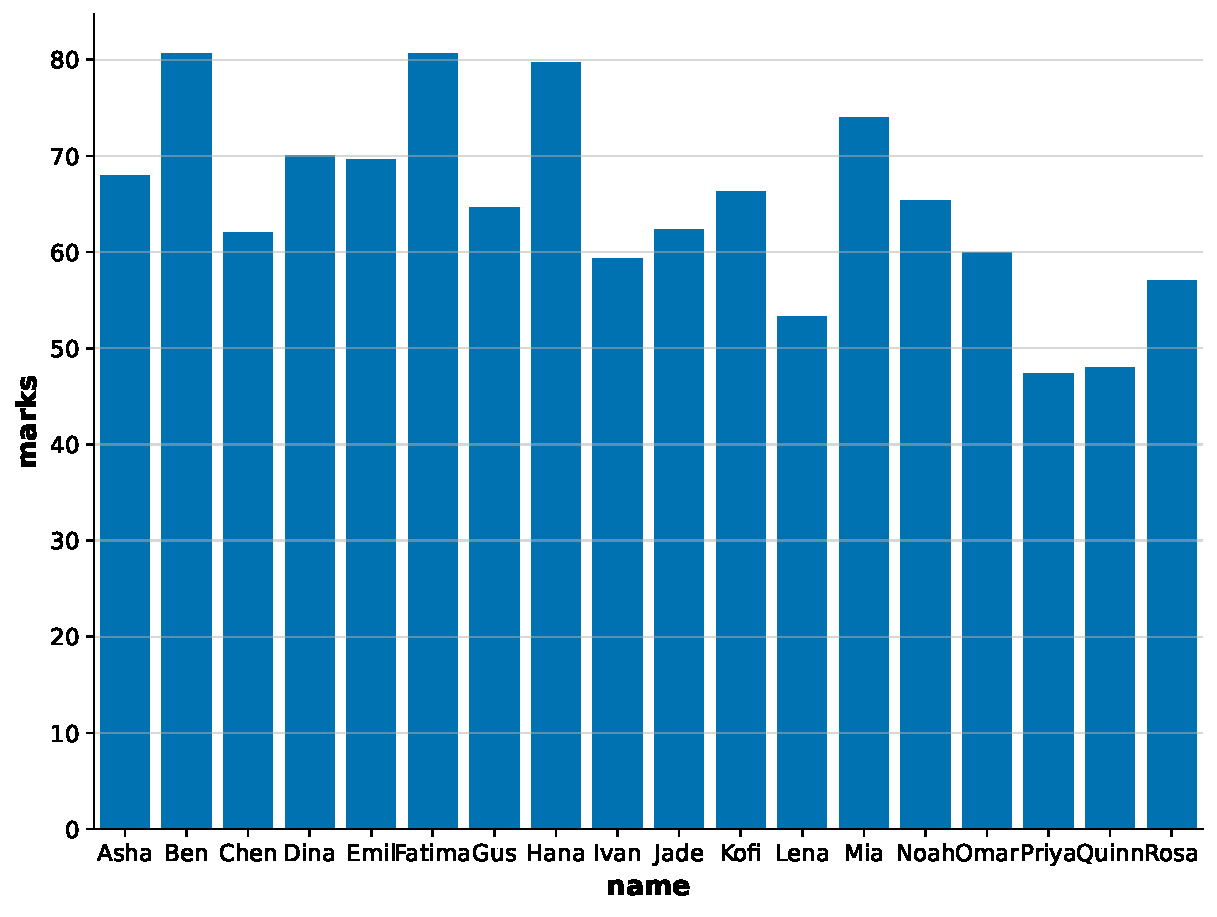
\includegraphics[width=0.72\textwidth,height=0.36\textheight,keepaspectratio]{figures/lesson01_example1_lesson1.pdf}
\captionof{figure}{Lesson 1, example: \code{lesson1.\allowbreak{}png}.}
\end{minipage}\end{center}
\begin{goodtoknow}
\begin{itemize}
  \item Chart types are nouns on a chart: \code{chart.\allowbreak{}bars}, \code{chart.\allowbreak{}lines}, \code{chart.\allowbreak{}dots} ... The chart is the thing, and bars is what it shows.
  \item For your own data, write chart = \code{sdata.\allowbreak{}chart(\textquotedbl{}my\_\allowbreak{}marks.\allowbreak{}xlsx\textquotedbl{})}. Excel, CSV, TSV, Parquet and JSON files all work.
  \item \code{chart.\allowbreak{}save(\textquotedbl{}lesson1.\allowbreak{}pdf\textquotedbl{})} saves a PDF instead: the end of the name decides the type.
  \item In Jupyter, VS Code or Spyder, write chart on the last line of a cell and the chart appears by itself. In a script, \code{chart.\allowbreak{}show()} opens it in a window.
  \item Are the names under the bars bumping into each other? Lesson 2 shows how to turn them.
\end{itemize}
\end{goodtoknow}
\begin{tryit}
\begin{enumerate}
  \item Change \code{x=\textquotedbl{}name\textquotedbl{}} to \code{x=\textquotedbl{}subject\textquotedbl{}}. What does each bar show now?
  \item Save the chart as \code{\textquotedbl{}my\_\allowbreak{}first\_\allowbreak{}chart.\allowbreak{}png\textquotedbl{}} and also as \code{\textquotedbl{}my\_\allowbreak{}first\_\allowbreak{}chart.\allowbreak{}pdf\textquotedbl{}}.
  \item Make a chart of the \code{\textquotedbl{}fruit\textquotedbl{}} table: bars with \code{x=\textquotedbl{}fruit\textquotedbl{}} and \code{y=\textquotedbl{}count\textquotedbl{}}.
\end{enumerate}
Worked solutions: page~\pageref{solutions:1}, or type \code{sdata.\allowbreak{}lesson(1,\allowbreak{} solutions=True)}.
\end{tryit}
\par\noindent{\small\sffamily\textbf{Words in this lesson:} \hyperref[word:sdata.example]{\code{sdata.\allowbreak{}example()}}, \hyperref[word:sdata.chart]{\code{sdata.\allowbreak{}chart()}}, \hyperref[word:bars]{\code{chart.\allowbreak{}bars()}}, \hyperref[word:save]{\code{chart.\allowbreak{}save()}}, \hyperref[word:show]{\code{chart.\allowbreak{}show()}}.\par}

\chapter{Titles and labels}\label{lesson:2}
\begin{learnbox}
\begin{itemize}
  \item how to put a title on top
  \item how to name the x-axis and the y-axis
  \item how to add a small caption and change the size of the text
\end{itemize}
\end{learnbox}
\section*{Example 1}
A chart is easier to read when it says what it shows. First draw, then add the words.
\begin{lstlisting}[style=py]
import simplydata as sdata
marks = sdata.example("marks")
chart = sdata.chart(marks)
chart.bars(x="name", y="marks")
chart.title_top("Our class marks")
chart.label_x("Student")
chart.label_y("Average mark")
chart.rotate_labels_x(45)
chart.caption_bottom("Made-up data from sdata.example")
chart.font_size(14)
chart.save("lesson2.png")
\end{lstlisting}
\whateachline
\begin{lineexplain}
  \item[1] Load simplydata.
  \item[2] Get the marks table.
  \item[3] Start a chart.
  \item[4] Draw one bar for each child.
  \item[5] Write a title on top of the chart.
  \item[6] Write a name under the x-axis (the bottom).
  \item[7] Write a name beside the y-axis (the side).
  \item[8] Turn the names under the bars by 45 degrees, so long names do not bump into each other.
  \item[9] Write a small line under the whole chart.
  \item[10] Make all the text a bit bigger (normal is 12).
  \item[11] Save it.
\end{lineexplain}
\printedoutput{output/lesson02_example1.txt}
\begin{center}\begin{minipage}{\linewidth}\centering
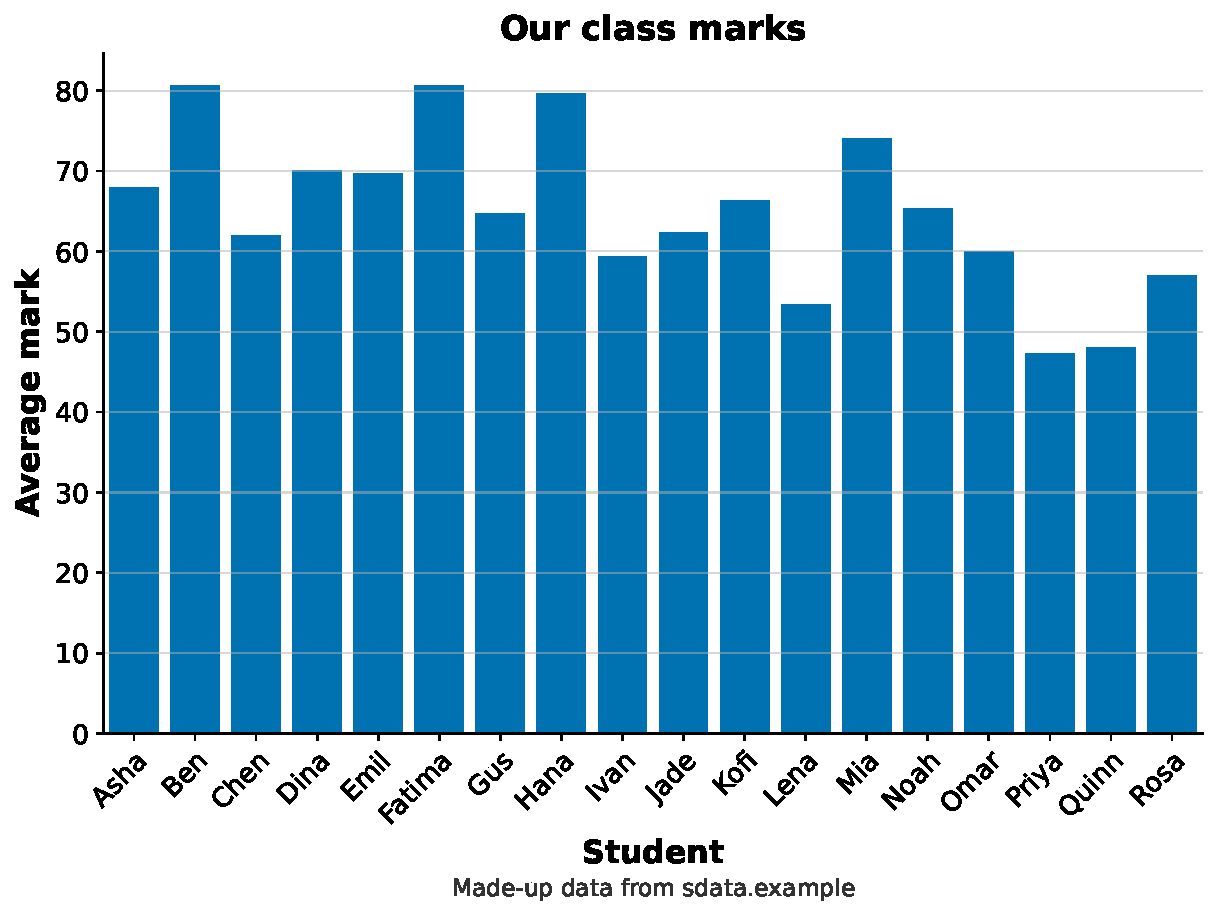
\includegraphics[width=0.72\textwidth,height=0.36\textheight,keepaspectratio]{figures/lesson02_example1_lesson2.pdf}
\captionof{figure}{Lesson 2, example 1: \code{lesson2.\allowbreak{}png}.}
\end{minipage}\end{center}
\section*{Example 2}
Words can also go next to the dots: a name for each dot, where it covers nothing.
\begin{lstlisting}[style=py]
import simplydata as sdata
kids = {"name": ["Asha", "Ben", "Chen", "Dina", "Eli"], "hours": [2.0, 5.5, 3.1, 7.2, 4.4], "marks": [48, 71, 55, 88, 62]}
chart = sdata.chart(kids)
chart.dots(x="hours", y="marks")
chart.names_on_dots("name")
chart.label_x("Hours of study")
chart.save("lesson2_names.png")
\end{lstlisting}
\whateachline
\begin{lineexplain}
  \item[1] Load simplydata.
  \item[2] A small table typed by hand: each column name, then its values in a list.
  \item[3] Start a chart of it.
  \item[4] One dot for each child.
  \item[5] Write each name next to its dot, where it covers no other name or dot. A name with no free place is left out, and a line says so.
  \item[6] Name the x-axis.
  \item[7] Save it.
\end{lineexplain}
\printedoutput{output/lesson02_example2.txt}
\begin{center}\begin{minipage}{\linewidth}\centering
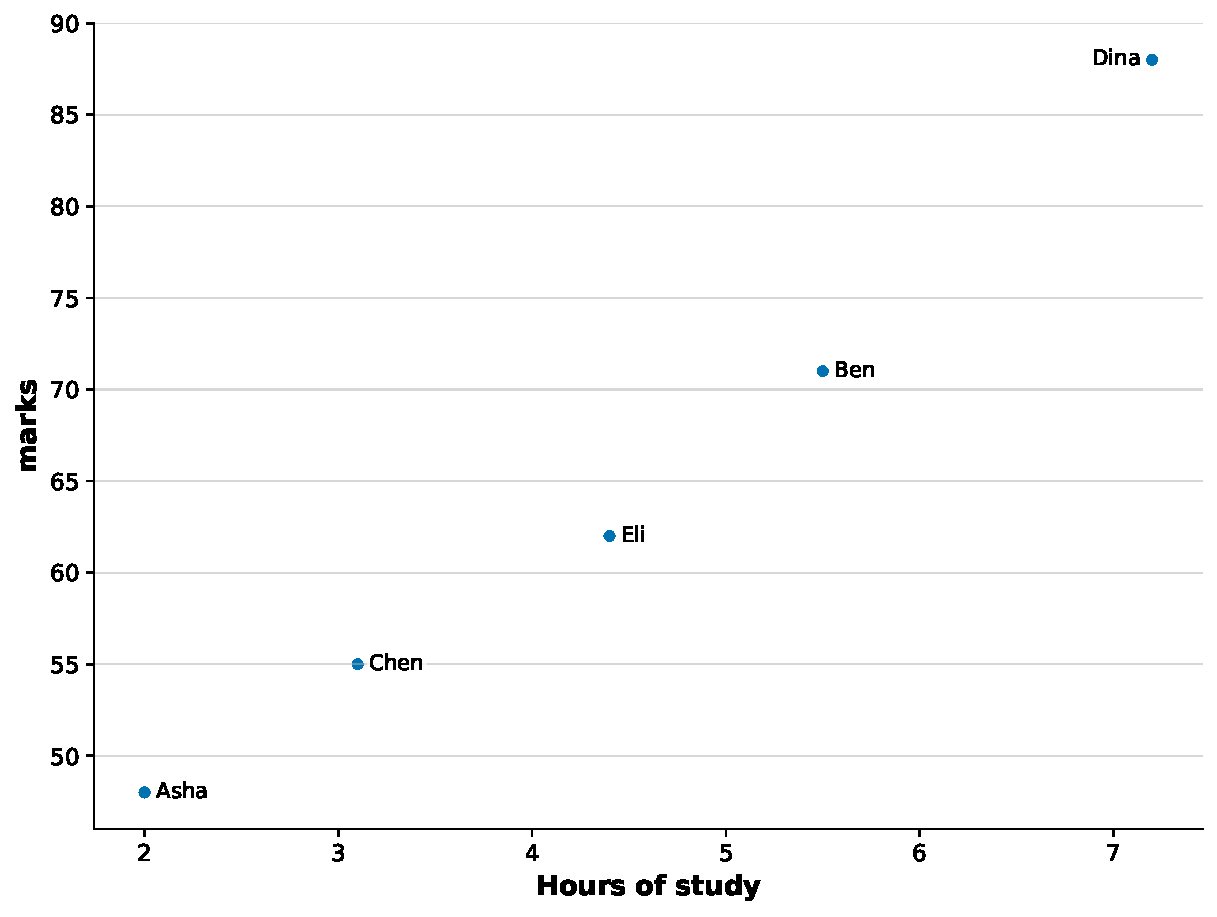
\includegraphics[width=0.72\textwidth,height=0.36\textheight,keepaspectratio]{figures/lesson02_example2_lesson2_names.pdf}
\captionof{figure}{Lesson 2, example 2: \code{lesson2\_\allowbreak{}names.\allowbreak{}png}.}
\end{minipage}\end{center}
\begin{goodtoknow}
\begin{itemize}
  \item After the chart type, the order of words such as \code{title\_\allowbreak{}top} and \code{label\_\allowbreak{}y} does not matter: the chart is drawn when you save or show it.
  \item Words that belong to one axis end in \_x or \_y: \code{label\_\allowbreak{}x}, \code{label\_\allowbreak{}y}, \code{rotate\_\allowbreak{}labels\_\allowbreak{}x}.
\end{itemize}
\end{goodtoknow}
\begin{tryit}
\begin{enumerate}
  \item Give the chart your own title, and label the y-axis \code{\textquotedbl{}Marks out of 100\textquotedbl{}}.
  \item Try \code{chart.\allowbreak{}font\_\allowbreak{}size(20)}. Then try 9. Which is easier to read?
  \item Take away the line \code{chart.\allowbreak{}rotate\_\allowbreak{}labels\_\allowbreak{}x(45)}. What happens to the names?
\end{enumerate}
Worked solutions: page~\pageref{solutions:2}, or type \code{sdata.\allowbreak{}lesson(2,\allowbreak{} solutions=True)}.
\end{tryit}
\par\noindent{\small\sffamily\textbf{Words in this lesson:} \hyperref[word:title-top]{\code{chart.\allowbreak{}title\_\allowbreak{}top()}}, \hyperref[word:label-x]{\code{chart.\allowbreak{}label\_\allowbreak{}x()}}, \hyperref[word:label-y]{\code{chart.\allowbreak{}label\_\allowbreak{}y()}}, \hyperref[word:rotate-labels-x]{\code{chart.\allowbreak{}rotate\_\allowbreak{}labels\_\allowbreak{}x()}}, \hyperref[word:caption-bottom]{\code{chart.\allowbreak{}caption\_\allowbreak{}bottom()}}, \hyperref[word:font-size]{\code{chart.\allowbreak{}font\_\allowbreak{}size()}}, \hyperref[word:names-on-dots]{\code{chart.\allowbreak{}names\_\allowbreak{}on\_\allowbreak{}dots()}}.\par}

\chapter{Colours, groups and legends}\label{lesson:3}
\begin{learnbox}
\begin{itemize}
  \item how to give each group its own colour
  \item how to choose your own colours
  \item how to move the legend (the box that says which colour is which)
  \item how to change the whole look with a style
\end{itemize}
\end{learnbox}
\section*{Example 1}
\code{colour=} inside a chart type splits the data into groups.
\begin{lstlisting}[style=py]
import simplydata as sdata
marks = sdata.example("marks")
chart = sdata.chart(marks)
chart.bars(x="subject", y="marks", colour="class")
chart.colours("orange", "teal", "purple")
chart.legend_bottom()
chart.title_top("Marks in each subject")
chart.save("lesson3_groups.png")
\end{lstlisting}
\whateachline
\begin{lineexplain}
  \item[1] Load simplydata.
  \item[2] Get the marks table.
  \item[3] Start a chart.
  \item[4] For each subject, draw one bar per class, each class in its own colour.
  \item[5] Choose the colours yourself, in order: class A orange, B teal, C purple.
  \item[6] Put the legend under the chart.
  \item[7] Add a title.
  \item[8] Save it.
\end{lineexplain}
\printedoutput{output/lesson03_example1.txt}
\begin{center}\begin{minipage}{\linewidth}\centering
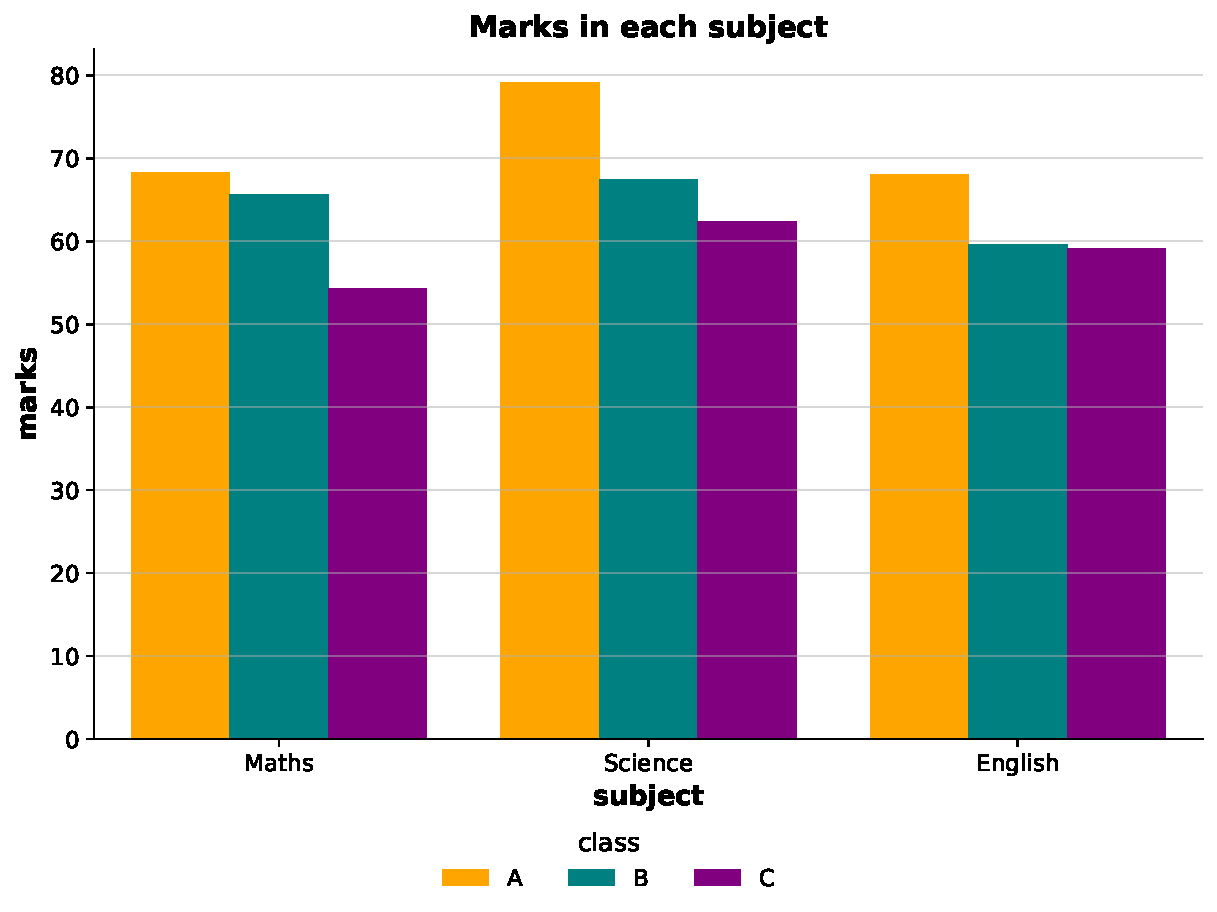
\includegraphics[width=0.72\textwidth,height=0.36\textheight,keepaspectratio]{figures/lesson03_example1_lesson3_groups.pdf}
\captionof{figure}{Lesson 3, example 1: \code{lesson3\_\allowbreak{}groups.\allowbreak{}png}.}
\end{minipage}\end{center}
\section*{Example 2}
Without groups, one colour is used for everything. You can choose it.
\begin{lstlisting}[style=py]
import simplydata as sdata
weather = sdata.example("weather")
chart = sdata.chart(weather)
chart.lines(x="month", y="rain")
chart.colour("blue")
chart.style("school")
chart.save("lesson3_look.png")
\end{lstlisting}
\whateachline
\begin{lineexplain}
  \item[1] Load simplydata.
  \item[2] Get the weather table: three made-up cities.
  \item[3] Start a chart.
  \item[4] Draw a line of rain through the months. With three cities in each month, the line shows their average.
  \item[5] Make the line blue.
  \item[6] Change the whole look. Try \code{\textquotedbl{}paper\textquotedbl{}}, \code{\textquotedbl{}school\textquotedbl{}}, \code{\textquotedbl{}presentation\textquotedbl{}} and \code{\textquotedbl{}dark\textquotedbl{}}.
  \item[7] Save it.
\end{lineexplain}
\printedoutput{output/lesson03_example2.txt}
\begin{center}\begin{minipage}{\linewidth}\centering
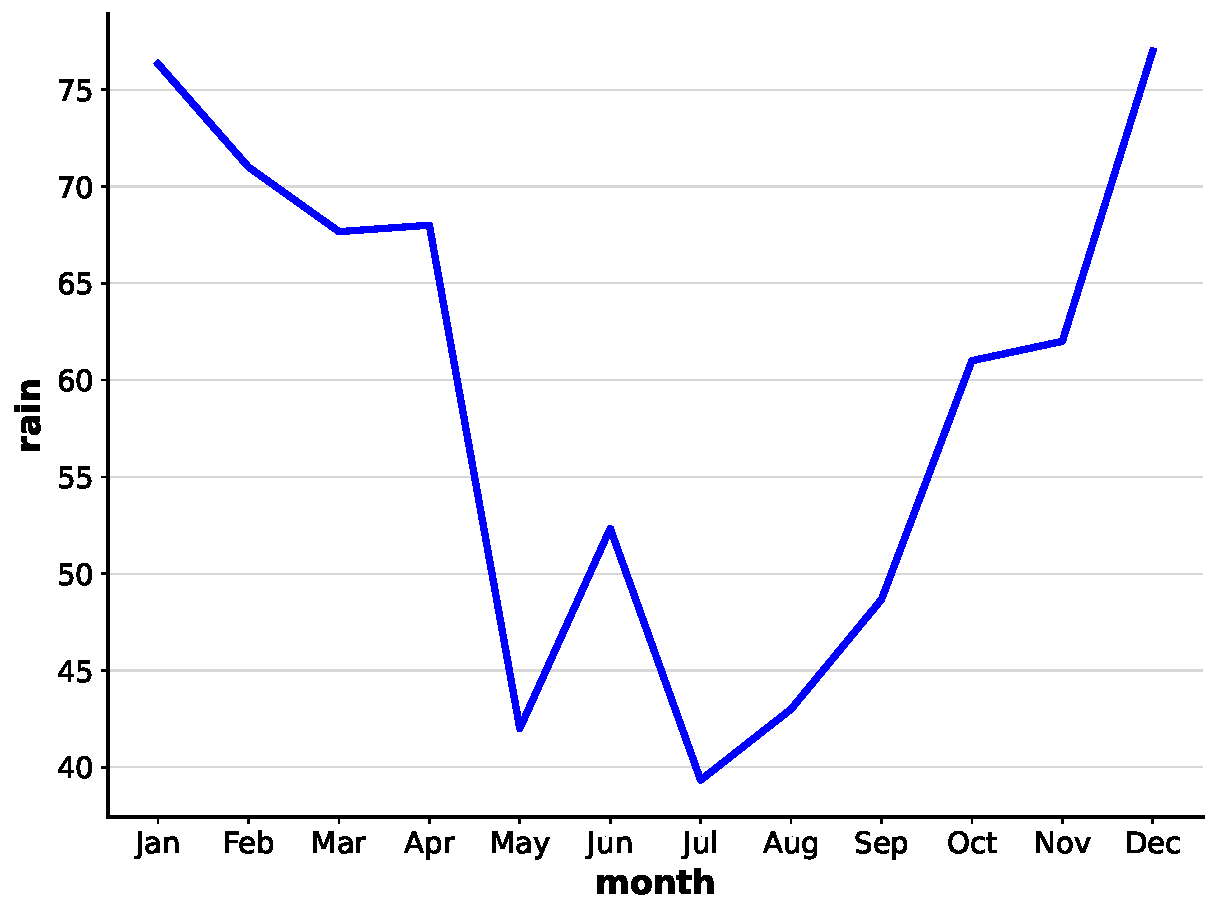
\includegraphics[width=0.72\textwidth,height=0.36\textheight,keepaspectratio]{figures/lesson03_example2_lesson3_look.pdf}
\captionof{figure}{Lesson 3, example 2: \code{lesson3\_\allowbreak{}look.\allowbreak{}png}.}
\end{minipage}\end{center}
\section*{Example 3}
Groups come in the order they first appear in the table. You can choose another order, and give the legend a name.
\begin{lstlisting}[style=py]
import simplydata as sdata
marks = sdata.example("marks")
chart = sdata.chart(marks)
chart.bars(x="class", y="marks", colour="subject")
chart.order_x("C", "B", "A")
chart.order_legend("Science", "Maths", "English")
chart.label_legend("Subject")
chart.save("lesson3_order.png")
\end{lstlisting}
\whateachline
\begin{lineexplain}
  \item[1] Load simplydata.
  \item[2] Get the marks table.
  \item[3] Start a chart.
  \item[4] For each class, one bar per subject.
  \item[5] Put the classes along the x-axis in this order.
  \item[6] Put the subjects in this order: in the legend and side by side in each class.
  \item[7] The name above the legend (normally the column name).
  \item[8] Save it.
\end{lineexplain}
\printedoutput{output/lesson03_example3.txt}
\begin{center}\begin{minipage}{\linewidth}\centering
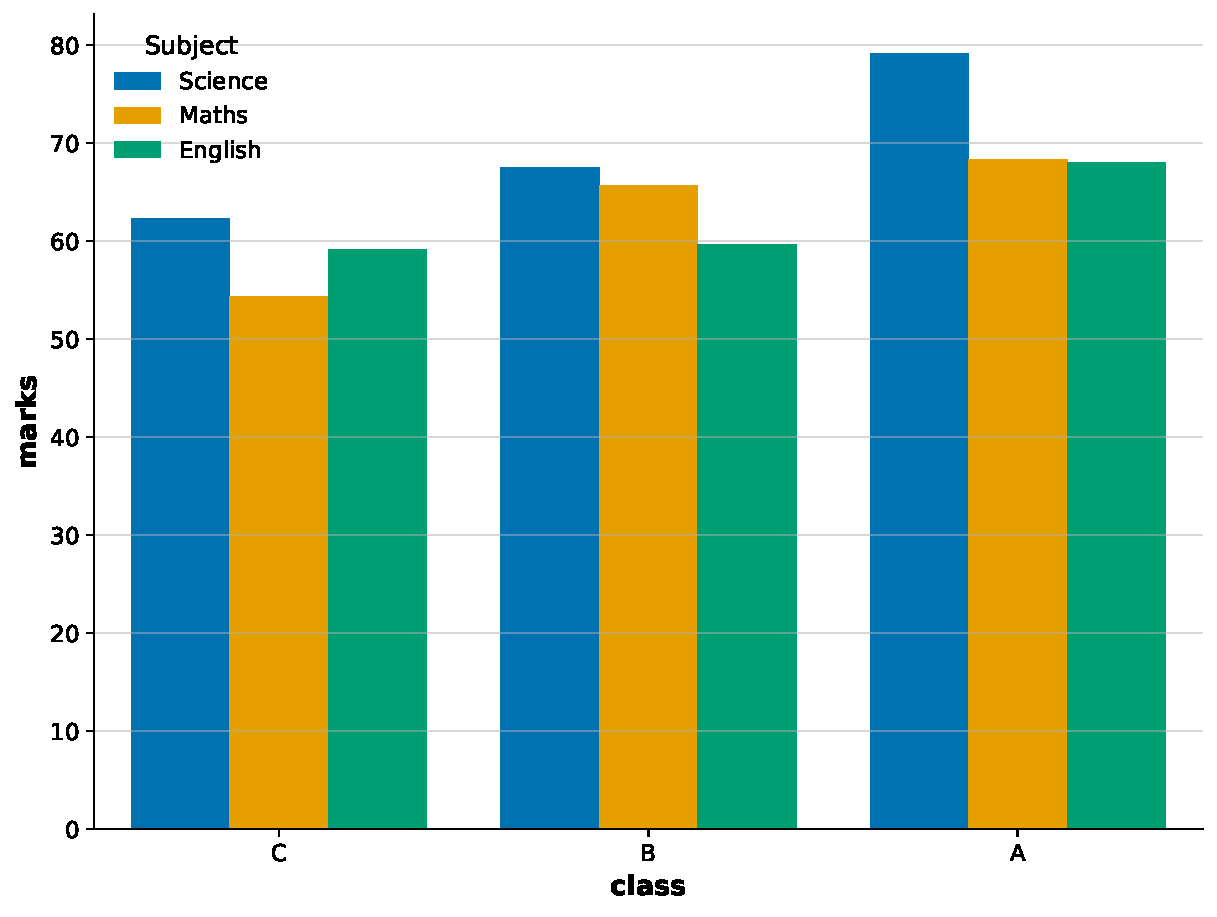
\includegraphics[width=0.72\textwidth,height=0.36\textheight,keepaspectratio]{figures/lesson03_example3_lesson3_order.pdf}
\captionof{figure}{Lesson 3, example 3: \code{lesson3\_\allowbreak{}order.\allowbreak{}png}.}
\end{minipage}\end{center}
\section*{Example 4}
Numbers can have colours too: a colour scale. And dots that overlap are easier to see when they let the others show through.
\begin{lstlisting}[style=py]
import simplydata as sdata
weather = sdata.example("weather")
chart = sdata.chart(weather)
chart.heatmap(x="month", y="city", value="temperature")
chart.colour_scale("blue to red", middle=10)
chart.save("lesson3_colour_scale.png")
marks = sdata.example("marks")
dots = sdata.chart(marks)
dots.dots(x="hours", y="marks", colour="class", transparency=0.5)
dots.save("lesson3_transparency.png")
\end{lstlisting}
\whateachline
\begin{lineexplain}
  \item[1] Load simplydata.
  \item[2] Get the weather table.
  \item[3] Start a chart.
  \item[4] One square per city and month, coloured by temperature.
  \item[5] Blue below 10 \textdegree{}C, red above, white at 10. \code{middle=} makes a scale that goes two ways.
  \item[6] Save it.
  \item[7] Get the marks table.
  \item[8] A second chart.
  \item[9] \code{transparency=0.\allowbreak{}5} makes each dot half see-through, so dots on top of each other show.
  \item[10] Save it.
\end{lineexplain}
\printedoutput{output/lesson03_example4.txt}
\begin{center}\begin{minipage}{\linewidth}\centering
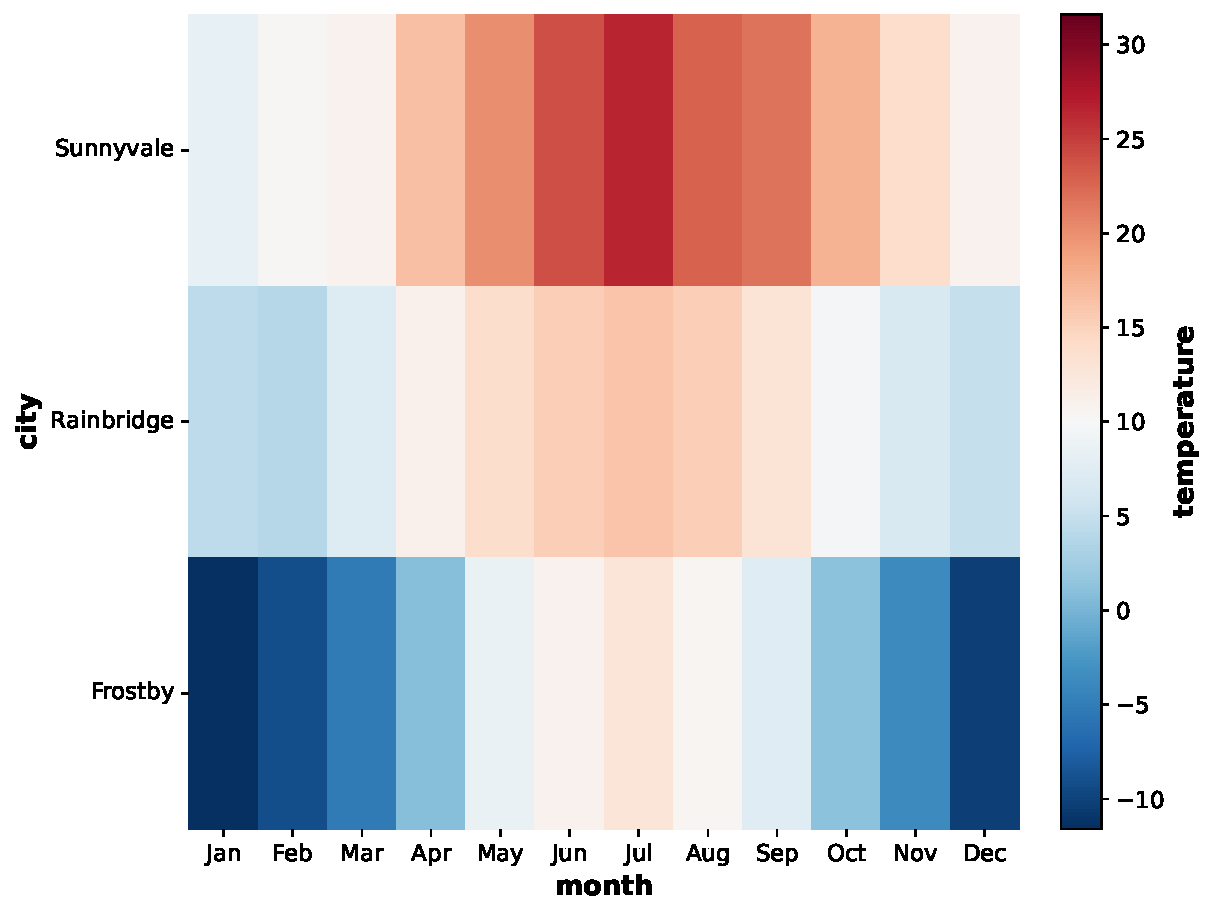
\includegraphics[width=0.48\textwidth,height=0.36\textheight,keepaspectratio]{figures/lesson03_example4_lesson3_colour_scale.pdf}\hfill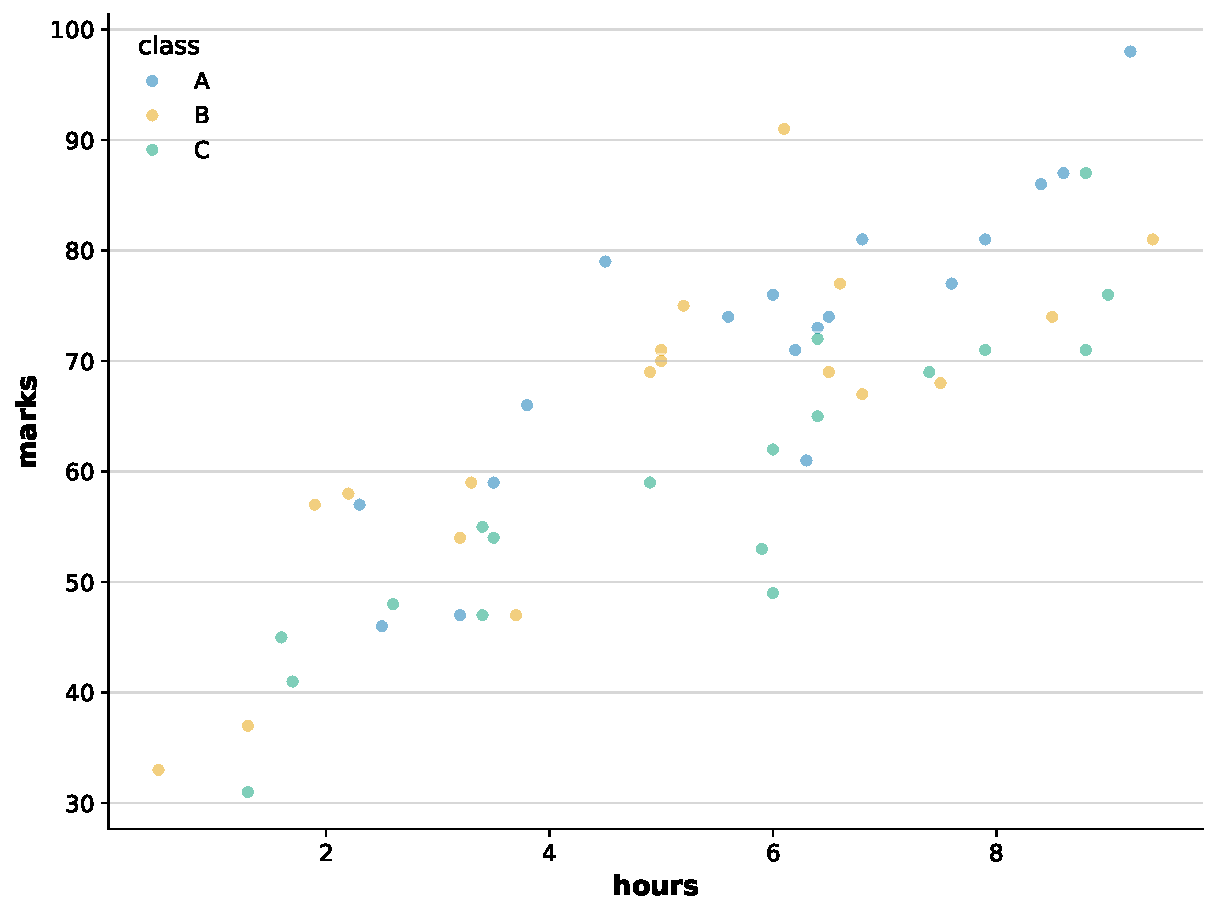
\includegraphics[width=0.48\textwidth,height=0.36\textheight,keepaspectratio]{figures/lesson03_example4_lesson3_transparency.pdf}
\captionof{figure}{Lesson 3, example 4: \code{lesson3\_\allowbreak{}colour\_\allowbreak{}scale.\allowbreak{}png} and \code{lesson3\_\allowbreak{}transparency.\allowbreak{}png}.}
\end{minipage}\end{center}
\begin{goodtoknow}
\begin{itemize}
  \item \code{colour=\textquotedbl{}class\textquotedbl{}} (a column) gives each group a colour. \code{colour=\textquotedbl{}red\textquotedbl{}} (a colour) makes that step red. color works too.
  \item The legend can go on any side: \code{legend\_\allowbreak{}top}, \code{legend\_\allowbreak{}bottom}, \code{legend\_\allowbreak{}left}, \code{legend\_\allowbreak{}right}. \code{hide\_\allowbreak{}legend} takes it away and \code{show\_\allowbreak{}legend} brings it back.
  \item Month and weekday names (\code{\textquotedbl{}Jan\textquotedbl{}}, \code{\textquotedbl{}Monday\textquotedbl{}}) come in calendar order by themselves, also in the small charts of \code{one\_\allowbreak{}chart\_\allowbreak{}per} and the frames of animate. \code{order\_\allowbreak{}x(biggest\_\allowbreak{}first=True)} puts the biggest bar first, and \code{order\_\allowbreak{}y} orders the groups up the y-axis.
\end{itemize}
\end{goodtoknow}
\begin{tryit}
\begin{enumerate}
  \item In the weather chart, add \code{colour=\textquotedbl{}city\textquotedbl{}} to \code{chart.\allowbreak{}lines(.\allowbreak{}.\allowbreak{}.\allowbreak{})}. How many lines do you get?
  \item Move the legend to the top with \code{chart.\allowbreak{}legend\_\allowbreak{}top()}.
  \item Try \code{chart.\allowbreak{}style(\textquotedbl{}dark\textquotedbl{})} and choose three colours that look good on it.
\end{enumerate}
Worked solutions: page~\pageref{solutions:3}, or type \code{sdata.\allowbreak{}lesson(3,\allowbreak{} solutions=True)}.
\end{tryit}
\par\noindent{\small\sffamily\textbf{Words in this lesson:} \hyperref[word:colours]{\code{chart.\allowbreak{}colours()}}, \hyperref[word:colour]{\code{chart.\allowbreak{}colour()}}, \hyperref[word:colour-scale]{\code{chart.\allowbreak{}colour\_\allowbreak{}scale()}}, \hyperref[word:legend-bottom]{\code{chart.\allowbreak{}legend\_\allowbreak{}bottom()}}, \hyperref[word:legend-top]{\code{chart.\allowbreak{}legend\_\allowbreak{}top()}}, \hyperref[word:hide-legend]{\code{chart.\allowbreak{}hide\_\allowbreak{}legend()}}, \hyperref[word:style]{\code{chart.\allowbreak{}style()}}, \hyperref[word:lines]{\code{chart.\allowbreak{}lines()}}, \hyperref[word:order-x]{\code{chart.\allowbreak{}order\_\allowbreak{}x()}}, \hyperref[word:order-legend]{\code{chart.\allowbreak{}order\_\allowbreak{}legend()}}, \hyperref[word:label-legend]{\code{chart.\allowbreak{}label\_\allowbreak{}legend()}}.\par}

\chapter{Different chart types}\label{lesson:4}
\begin{learnbox}
\begin{itemize}
  \item lines, dots, histograms, boxes and pies
  \item which chart suits which question
  \item how to put two chart types on top of each other
\end{itemize}
\end{learnbox}
\section*{Example 1}
Lines show how something changes, for example over time.
\begin{lstlisting}[style=py]
import simplydata as sdata
weather = sdata.example("weather")
chart = sdata.chart(weather)
chart.lines(x="month", y="temperature", colour="city", dots=True)
chart.save("lesson4_lines.png")
\end{lstlisting}
\whateachline
\begin{lineexplain}
  \item[1] Load simplydata.
  \item[2] Get the weather table.
  \item[3] Start a chart.
  \item[4] One line per city. \code{dots=True} also marks each month with a dot.
  \item[5] Save it.
\end{lineexplain}
\printedoutput{output/lesson04_example1.txt}
\begin{center}\begin{minipage}{\linewidth}\centering
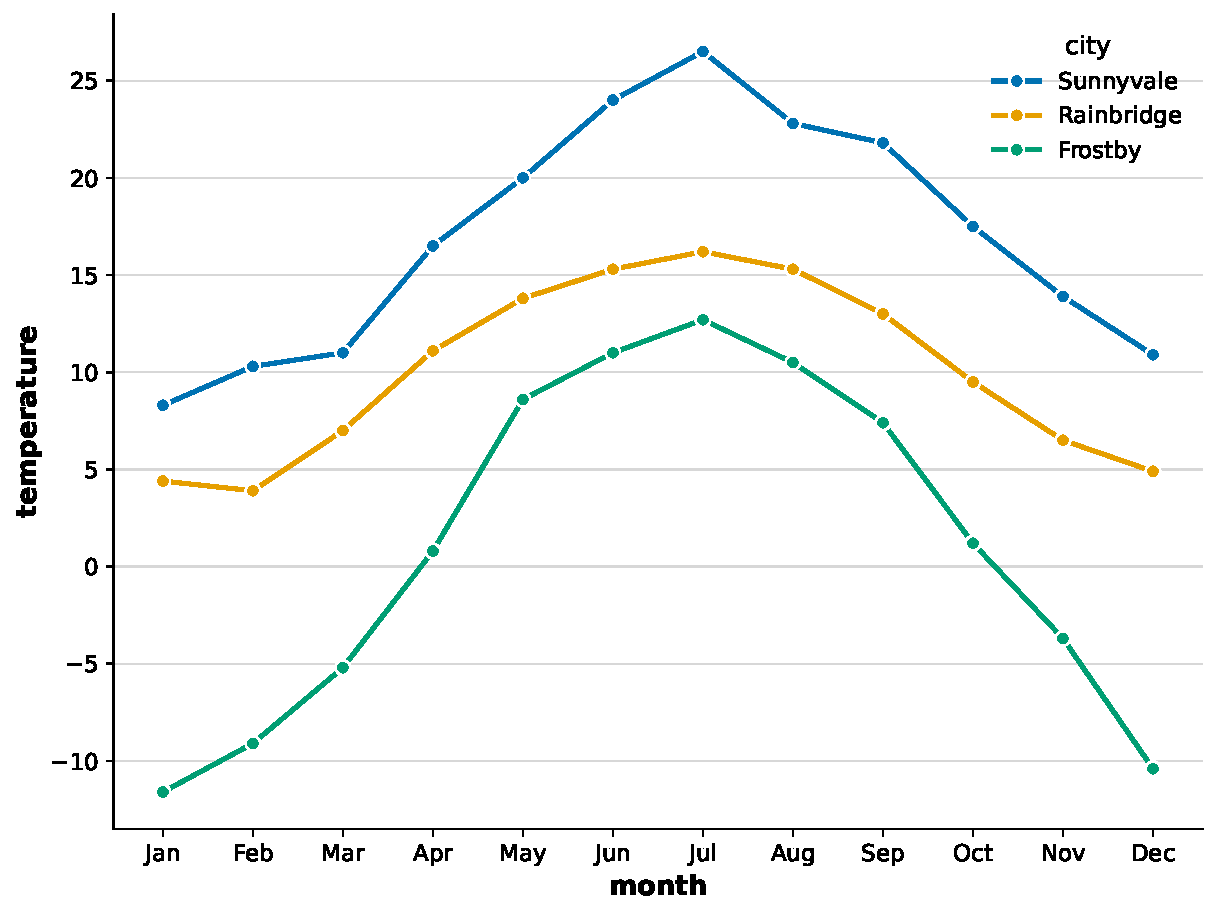
\includegraphics[width=0.72\textwidth,height=0.36\textheight,keepaspectratio]{figures/lesson04_example1_lesson4_lines.pdf}
\captionof{figure}{Lesson 4, example 1: \code{lesson4\_\allowbreak{}lines.\allowbreak{}png}.}
\end{minipage}\end{center}
\section*{Example 2}
Dots show if two things go together. This is also called a scatter chart.
\begin{lstlisting}[style=py]
import simplydata as sdata
marks = sdata.example("marks")
chart = sdata.chart(marks)
chart.dots(x="hours", y="marks", colour="class")
chart.save("lesson4_dots.png")
\end{lstlisting}
\whateachline
\begin{lineexplain}
  \item[1] Load simplydata.
  \item[2] Get the marks table.
  \item[3] Start a chart.
  \item[4] One dot for each test: how long the child studied, and the mark they got.
  \item[5] Save it. Do more hours give more marks?
\end{lineexplain}
\printedoutput{output/lesson04_example2.txt}
\begin{center}\begin{minipage}{\linewidth}\centering
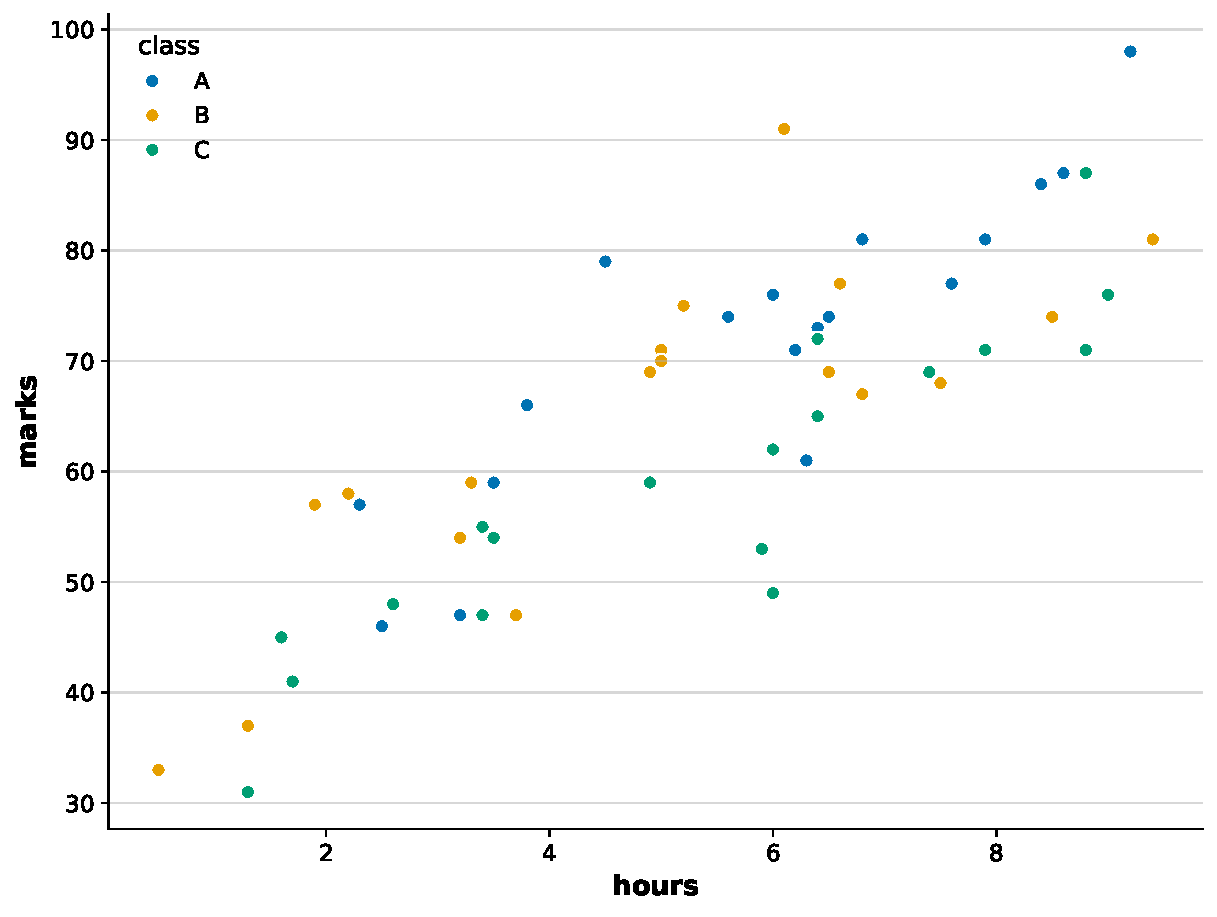
\includegraphics[width=0.72\textwidth,height=0.36\textheight,keepaspectratio]{figures/lesson04_example2_lesson4_dots.pdf}
\captionof{figure}{Lesson 4, example 2: \code{lesson4\_\allowbreak{}dots.\allowbreak{}png}.}
\end{minipage}\end{center}
\section*{Example 3}
A histogram counts how many values fall in each range, like 40 to 50, 50 to 60 ... Its shape is called the distribution of the values.
\begin{lstlisting}[style=py]
import simplydata as sdata
marks = sdata.example("marks")
chart = sdata.chart(marks)
chart.histogram(x="marks", bins=8)
chart.save("lesson4_histogram.png")
\end{lstlisting}
\whateachline
\begin{lineexplain}
  \item[1] Load simplydata.
  \item[2] Get the marks table.
  \item[3] Start a chart.
  \item[4] Cut the marks into 8 ranges (bins) and draw a bar for how many marks are in each.
  \item[5] Save it.
\end{lineexplain}
\printedoutput{output/lesson04_example3.txt}
\begin{center}\begin{minipage}{\linewidth}\centering
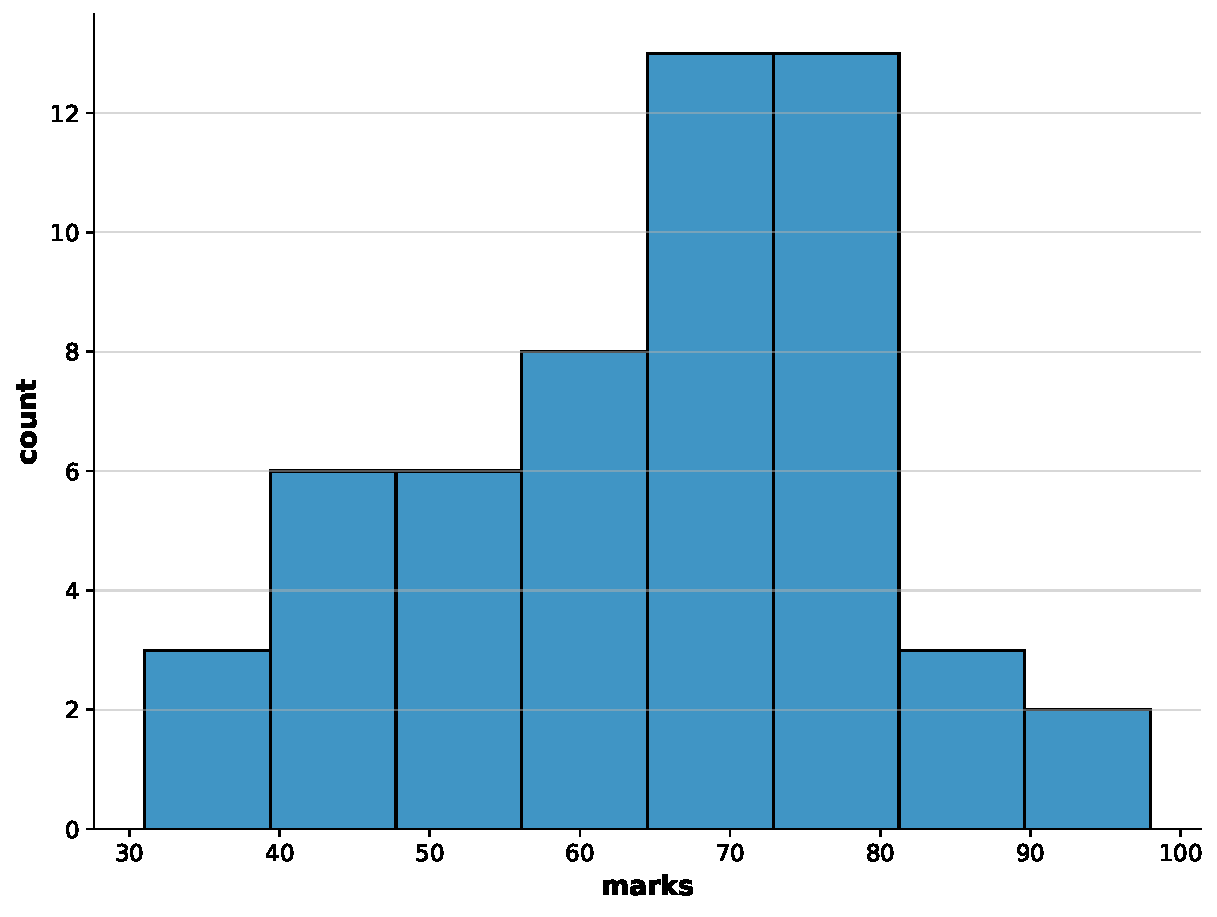
\includegraphics[width=0.72\textwidth,height=0.36\textheight,keepaspectratio]{figures/lesson04_example3_lesson4_histogram.pdf}
\captionof{figure}{Lesson 4, example 3: \code{lesson4\_\allowbreak{}histogram.\allowbreak{}png}.}
\end{minipage}\end{center}
\section*{Example 4}
Boxes show how spread out the values are. Two chart types on one chart are drawn one on top of the other.
\begin{lstlisting}[style=py]
import simplydata as sdata
marks = sdata.example("marks")
chart = sdata.chart(marks)
chart.boxes(x="class", y="marks")
chart.all_dots(x="class", y="marks")
chart.save("lesson4_boxes.png")
\end{lstlisting}
\whateachline
\begin{lineexplain}
  \item[1] Load simplydata.
  \item[2] Get the marks table.
  \item[3] Start a chart.
  \item[4] One box per class. The line in the box is the median: the middle mark when they are put in order. The box holds the middle half of the marks (the interquartile range).
  \item[5] Also show every single mark as a dot, on top of the boxes.
  \item[6] Save it.
\end{lineexplain}
\printedoutput{output/lesson04_example4.txt}
\begin{center}\begin{minipage}{\linewidth}\centering
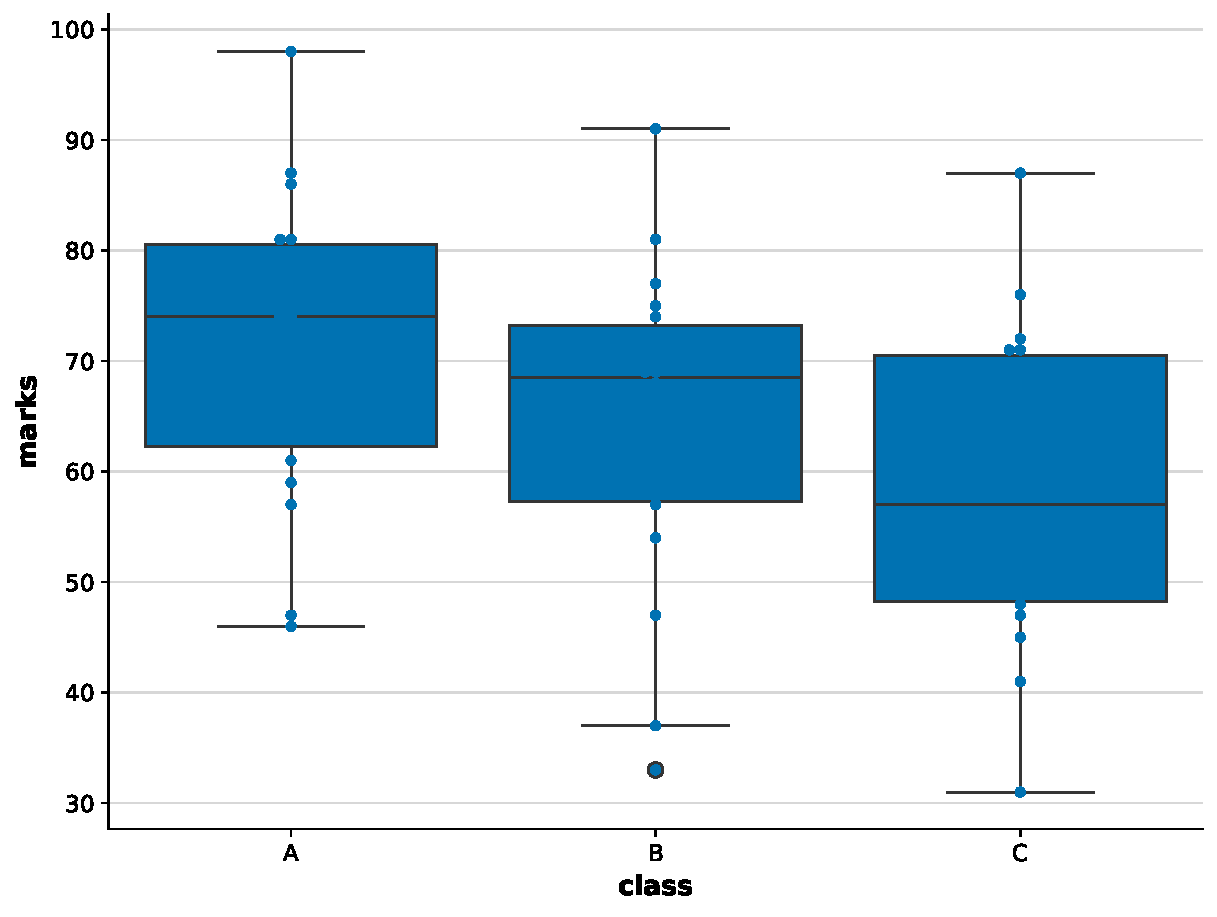
\includegraphics[width=0.72\textwidth,height=0.36\textheight,keepaspectratio]{figures/lesson04_example4_lesson4_boxes.pdf}
\captionof{figure}{Lesson 4, example 4: \code{lesson4\_\allowbreak{}boxes.\allowbreak{}png}.}
\end{minipage}\end{center}
\section*{Example 5}
A pie shows how a whole is shared out.
\begin{lstlisting}[style=py]
import simplydata as sdata
fruit = sdata.example("fruit")
chart = sdata.chart(fruit)
chart.pie(labels="fruit", values="count")
chart.save("lesson4_pie.png")
\end{lstlisting}
\whateachline
\begin{lineexplain}
  \item[1] Load simplydata.
  \item[2] Get the fruit table: what two shops sold in a week.
  \item[3] Start a chart.
  \item[4] One slice per fruit, as big as the number sold.
  \item[5] Save it.
\end{lineexplain}
\printedoutput{output/lesson04_example5.txt}
\begin{center}\begin{minipage}{\linewidth}\centering
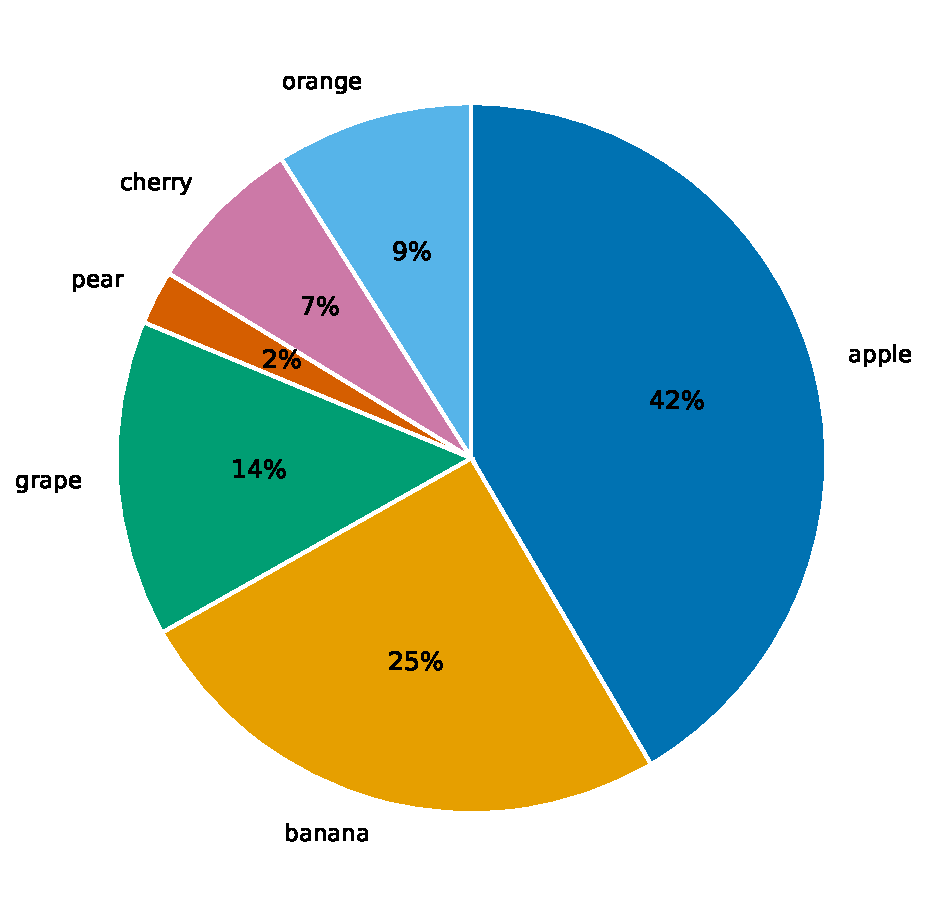
\includegraphics[width=0.72\textwidth,height=0.36\textheight,keepaspectratio]{figures/lesson04_example5_lesson4_pie.pdf}
\captionof{figure}{Lesson 4, example 5: \code{lesson4\_\allowbreak{}pie.\allowbreak{}png}.}
\end{minipage}\end{center}
\begin{goodtoknow}
\begin{itemize}
  \item Chart types on the same chart are layers of one chart. Lesson 7 shows how to make several charts and put them on one page.
  \item There are more chart types: area, violins, heatmap, polar, contour, surface and \code{dots\_\allowbreak{}3d}. Type \code{sdata.\allowbreak{}words()} to see them all and \code{sdata.\allowbreak{}help(\textquotedbl{}violins\textquotedbl{})} to learn one.
\end{itemize}
\end{goodtoknow}
\begin{tryit}
\begin{enumerate}
  \item Draw \code{chart.\allowbreak{}violins(x=\textquotedbl{}class\textquotedbl{},\allowbreak{} y=\textquotedbl{}marks\textquotedbl{})} instead of boxes. What is different?
  \item Draw a histogram of the weather \code{\textquotedbl{}temperature\textquotedbl{}} column with \code{bins=6}.
  \item Make a chart of \code{sdata.\allowbreak{}example(\textquotedbl{}growth\textquotedbl{})} and draw \code{chart.\allowbreak{}area(x=\textquotedbl{}year\textquotedbl{},\allowbreak{} y=\textquotedbl{}population\textquotedbl{},\allowbreak{} colour=\textquotedbl{}country\textquotedbl{})}.
\end{enumerate}
Worked solutions: page~\pageref{solutions:4}, or type \code{sdata.\allowbreak{}lesson(4,\allowbreak{} solutions=True)}.
\end{tryit}
\par\noindent{\small\sffamily\textbf{Words in this lesson:} \hyperref[word:lines]{\code{chart.\allowbreak{}lines()}}, \hyperref[word:dots]{\code{chart.\allowbreak{}dots()}}, \hyperref[word:histogram]{\code{chart.\allowbreak{}histogram()}}, \hyperref[word:boxes]{\code{chart.\allowbreak{}boxes()}}, \hyperref[word:all-dots]{\code{chart.\allowbreak{}all\_\allowbreak{}dots()}}, \hyperref[word:pie]{\code{chart.\allowbreak{}pie()}}, \hyperref[word:violins]{\code{chart.\allowbreak{}violins()}}, \hyperref[word:area]{\code{chart.\allowbreak{}area()}}.\par}

\chapter{Statistics: averages, error bars and fit lines}\label{lesson:5}
\begin{learnbox}
\begin{itemize}
  \item what a bar shows when a group has many values: the average or the median
  \item how to add error bars, and the difference between standard deviation and standard error
  \item how to draw the straight line that fits some dots best
\end{itemize}
\end{learnbox}
\section*{Example 1}
The average (also called the mean) is all the values added up, divided by how many there are. Error bars show how far the values spread around it.
\begin{lstlisting}[style=py]
import simplydata as sdata
marks = sdata.example("marks")
chart = sdata.chart(marks)
chart.bars(x="class", y="marks", show="average", error="standard deviation")
chart.numbers_on_bars()
chart.save("lesson5_average.png")
\end{lstlisting}
\whateachline
\begin{lineexplain}
  \item[1] Load simplydata.
  \item[2] Get the marks table.
  \item[3] Start a chart.
  \item[4] One bar per class, as tall as the average mark. The error bars show the standard deviation: how far marks usually are from the average. A line is printed that says which error bars were drawn.
  \item[5] Write the average on each bar.
  \item[6] Save it.
\end{lineexplain}
\printedoutput{output/lesson05_example1.txt}
\begin{center}\begin{minipage}{\linewidth}\centering
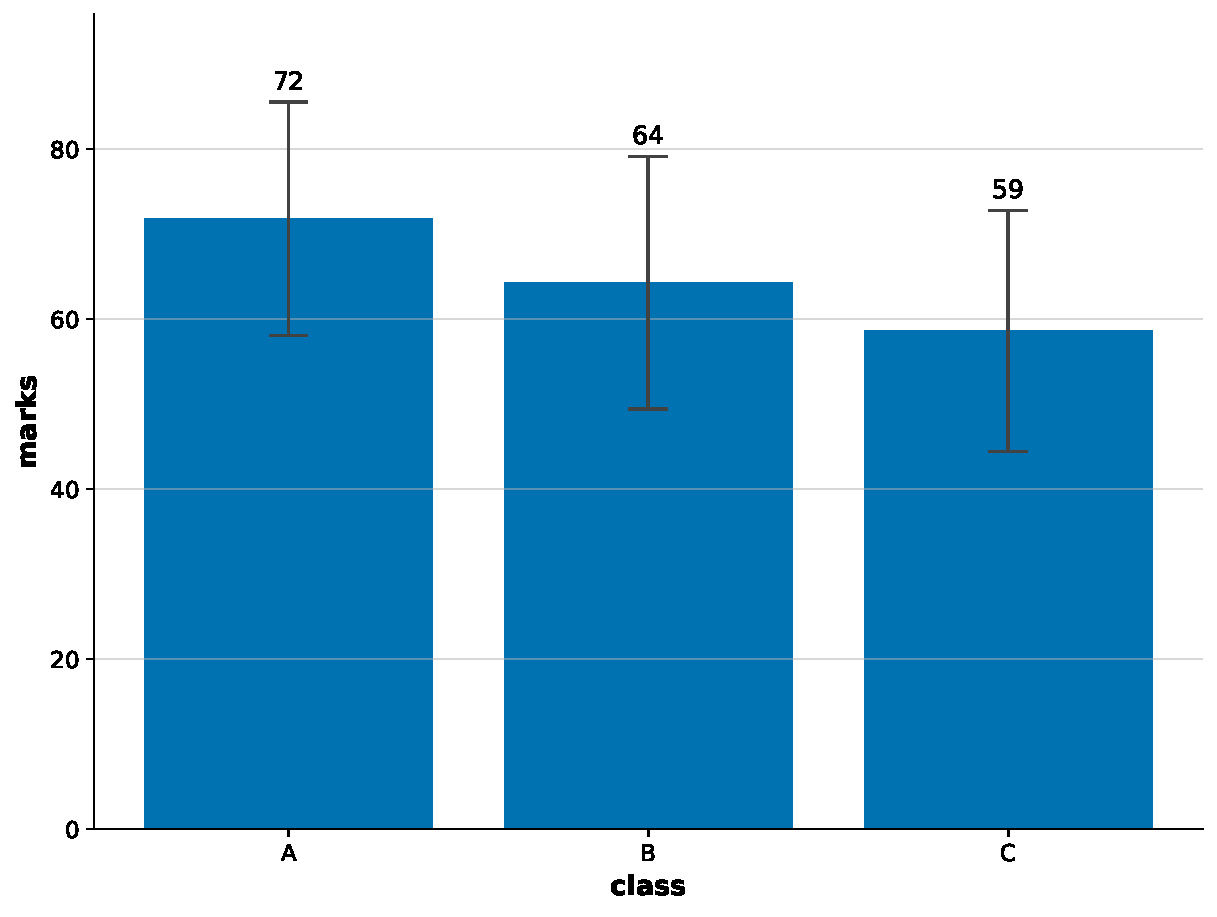
\includegraphics[width=0.72\textwidth,height=0.36\textheight,keepaspectratio]{figures/lesson05_example1_lesson5_average.pdf}
\captionof{figure}{Lesson 5, example 1: \code{lesson5\_\allowbreak{}average.\allowbreak{}png}.}
\end{minipage}\end{center}
\section*{Example 2}
A fit line is the straight line that goes as close as possible to all the dots.
\begin{lstlisting}[style=py]
import simplydata as sdata
marks = sdata.example("marks")
chart = sdata.chart(marks)
chart.dots(x="hours", y="marks")
chart.fit_line(confidence_band=True, show_equation=True)
chart.save("lesson5_fit.png")
\end{lstlisting}
\whateachline
\begin{lineexplain}
  \item[1] Load simplydata.
  \item[2] Get the marks table.
  \item[3] Start a chart.
  \item[4] One dot per test: hours of study and the mark.
  \item[5] Add the best straight line (also called linear regression). \code{confidence\_\allowbreak{}band=True} shades where the true line very likely is (the 95 \% confidence interval). \code{show\_\allowbreak{}equation=True} writes its equation and R\textsuperscript{2} (1 means the dots sit right on the line, 0 means no pattern at all).
  \item[6] Save it.
\end{lineexplain}
\printedoutput{output/lesson05_example2.txt}
\begin{center}\begin{minipage}{\linewidth}\centering
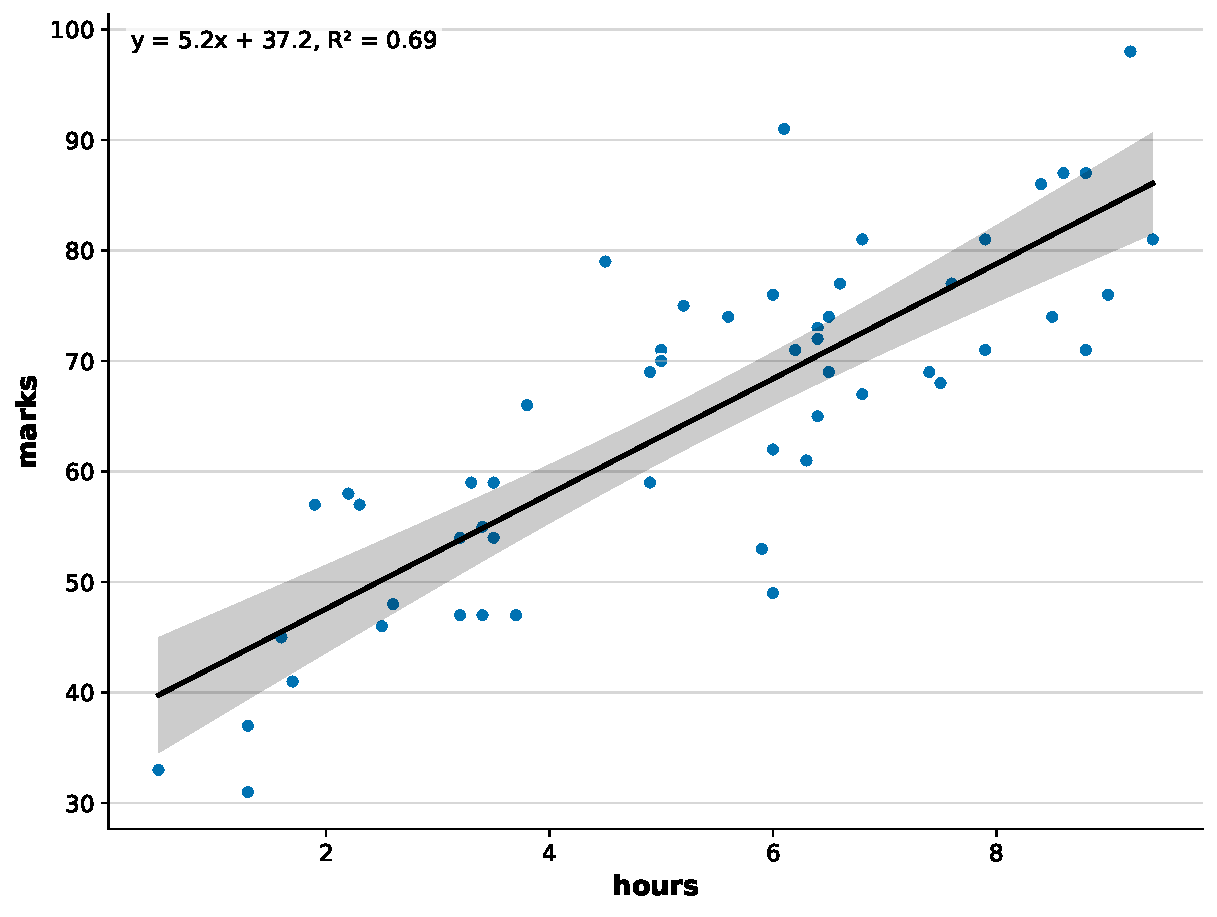
\includegraphics[width=0.72\textwidth,height=0.36\textheight,keepaspectratio]{figures/lesson05_example2_lesson5_fit.pdf}
\captionof{figure}{Lesson 5, example 2: \code{lesson5\_\allowbreak{}fit.\allowbreak{}png}.}
\end{minipage}\end{center}
\section*{Example 3}
A density curve is a smooth histogram: high where many values are.
\begin{lstlisting}[style=py]
import simplydata as sdata
marks = sdata.example("marks")
chart = sdata.chart(marks)
chart.density(x="marks", colour="class")
chart.save("lesson5_density.png")
\end{lstlisting}
\whateachline
\begin{lineexplain}
  \item[1] Load simplydata.
  \item[2] Get the marks table.
  \item[3] Start a chart.
  \item[4] One smooth curve for each class (a kernel density estimate).
  \item[5] Save it.
\end{lineexplain}
\printedoutput{output/lesson05_example3.txt}
\begin{center}\begin{minipage}{\linewidth}\centering
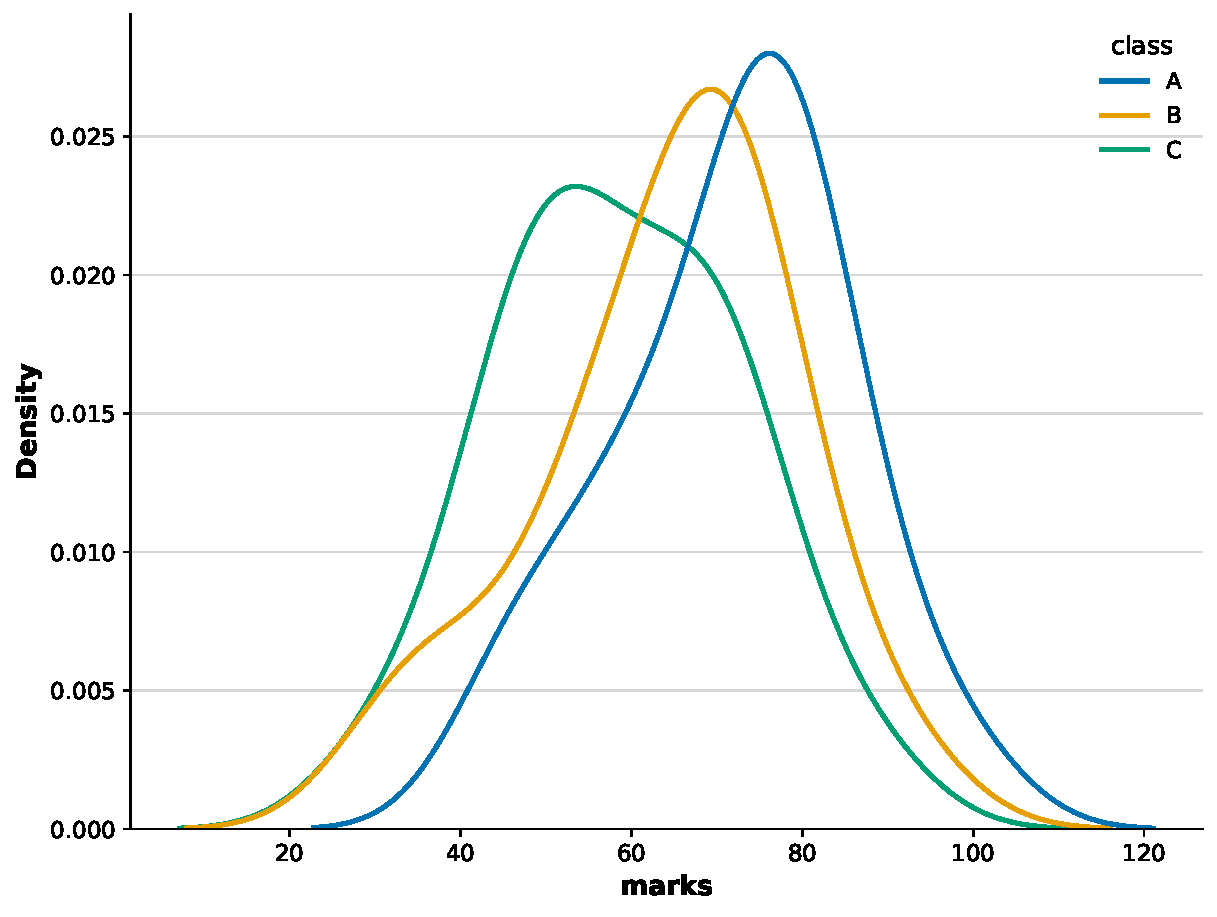
\includegraphics[width=0.72\textwidth,height=0.36\textheight,keepaspectratio]{figures/lesson05_example3_lesson5_density.pdf}
\captionof{figure}{Lesson 5, example 3: \code{lesson5\_\allowbreak{}density.\allowbreak{}png}.}
\end{minipage}\end{center}
\section*{Example 4}
Two more ways to see the shape of values: are they bell-shaped, and what share lies below each value?
\begin{lstlisting}[style=py]
import simplydata as sdata
marks = sdata.example("marks")
chart = sdata.chart(marks)
chart.qq_dots("marks")
chart.save("lesson5_qq.png")
shares = sdata.chart(marks)
shares.cumulative_share(x="marks", colour="class")
shares.save("lesson5_cumulative.png")
\end{lstlisting}
\whateachline
\begin{lineexplain}
  \item[1] Load simplydata.
  \item[2] Get the marks table.
  \item[3] Start a chart.
  \item[4] A Q-Q plot: if the marks follow a bell curve (normal), the dots lie close to the straight line.
  \item[5] Save it.
  \item[6] A second chart.
  \item[7] For each mark, the share of children with that mark or less (an ECDF). The class whose line is further right did better.
  \item[8] Save it.
\end{lineexplain}
\printedoutput{output/lesson05_example4.txt}
\begin{center}\begin{minipage}{\linewidth}\centering
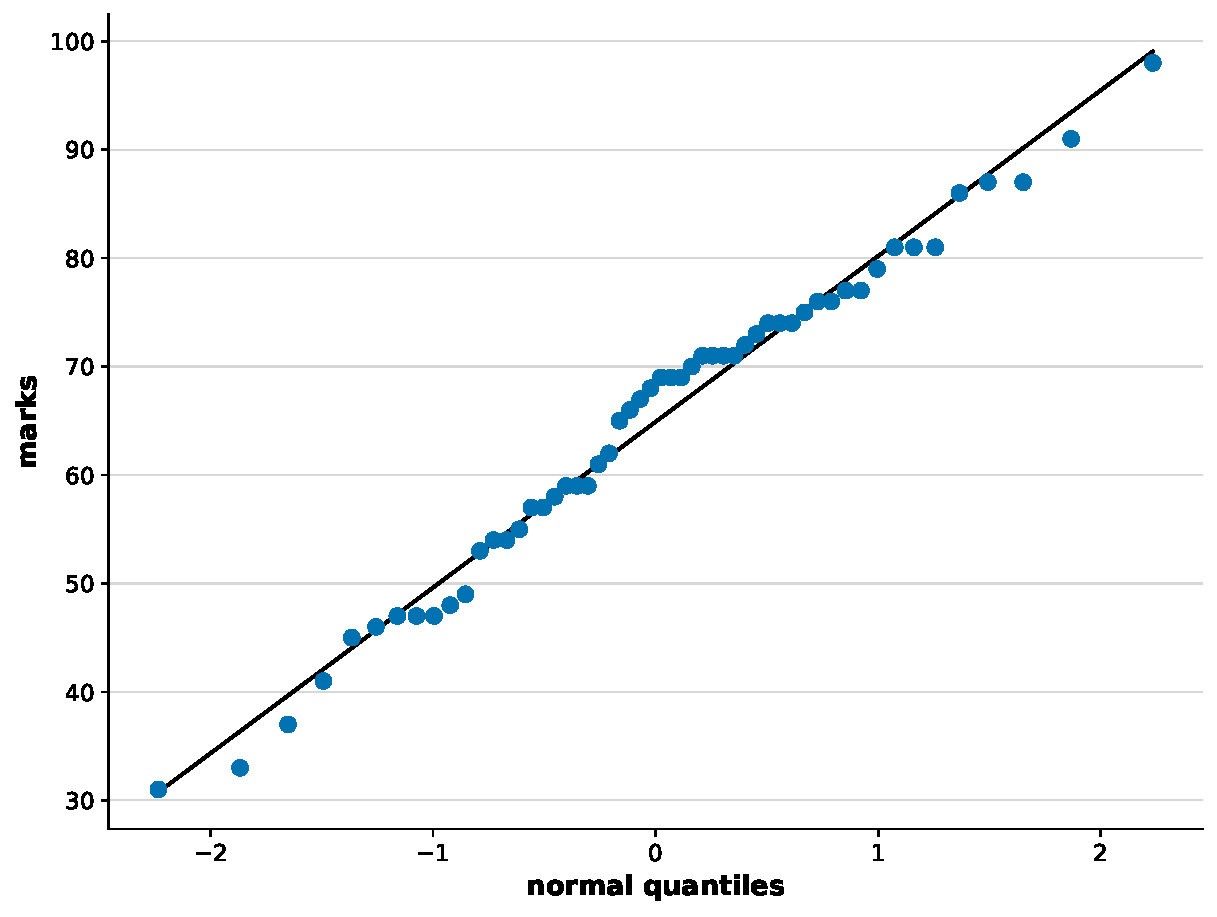
\includegraphics[width=0.48\textwidth,height=0.36\textheight,keepaspectratio]{figures/lesson05_example4_lesson5_qq.pdf}\hfill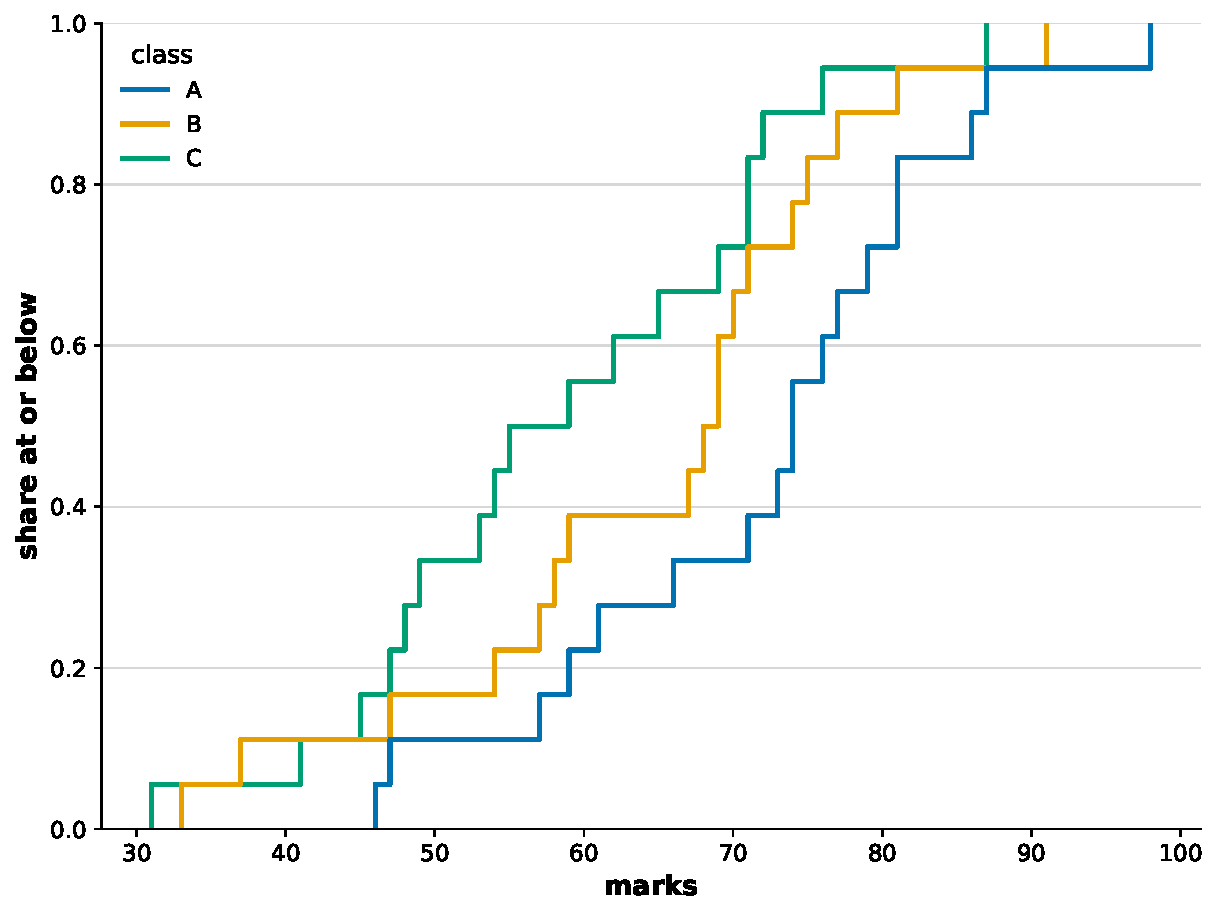
\includegraphics[width=0.48\textwidth,height=0.36\textheight,keepaspectratio]{figures/lesson05_example4_lesson5_cumulative.pdf}
\captionof{figure}{Lesson 5, example 4: \code{lesson5\_\allowbreak{}qq.\allowbreak{}png} and \code{lesson5\_\allowbreak{}cumulative.\allowbreak{}png}.}
\end{minipage}\end{center}
\begin{goodtoknow}
\begin{itemize}
  \item Average or median? The median is the middle value when the values are put in order. One very big or very small value pulls the average towards it, but hardly moves the median, so the median is safer when a few values are far from the rest (outliers).
  \item \code{show=} can be \code{\textquotedbl{}average\textquotedbl{}}, \code{\textquotedbl{}median\textquotedbl{}}, \code{\textquotedbl{}total\textquotedbl{}} (all added up), \code{\textquotedbl{}count\textquotedbl{}} (how many rows), \code{\textquotedbl{}smallest\textquotedbl{}}, \code{\textquotedbl{}biggest\textquotedbl{}} or \code{\textquotedbl{}standard deviation\textquotedbl{}}: the same names as the table words \code{average\_\allowbreak{}of}, \code{median\_\allowbreak{}of} and so on.
  \item Standard deviation or standard error? The standard deviation describes the values: how spread out they are. The standard error describes the average: how sure we are of it. It gets smaller as you collect more values, even when the values spread just as much.
  \item \code{error=\textquotedbl{}confidence interval\textquotedbl{}} draws the 95 \% confidence interval: the range the true average is very likely to be in. The short forms \code{\textquotedbl{}sd\textquotedbl{}}, \code{\textquotedbl{}se\textquotedbl{}} and \code{\textquotedbl{}ci\textquotedbl{}} work too. Always say in your caption which error bars you drew.
  \item \code{fit\_\allowbreak{}curve(degree=2)} fits a curve with one bend; \code{smooth\_\allowbreak{}line()} follows the dots freely.
\end{itemize}
\end{goodtoknow}
\begin{tryit}
\begin{enumerate}
  \item Change \code{show=\textquotedbl{}average\textquotedbl{}} to \code{show=\textquotedbl{}median\textquotedbl{}}. Do the bars change much?
  \item Change \code{error=\textquotedbl{}standard deviation\textquotedbl{}} to \code{error=\textquotedbl{}standard error\textquotedbl{}}. Are the error bars bigger or smaller? Why?
  \item Make a chart of the weather table, draw dots with \code{x=\textquotedbl{}month\_\allowbreak{}number\textquotedbl{}}, \code{y=\textquotedbl{}temperature\textquotedbl{}} and add \code{chart.\allowbreak{}fit\_\allowbreak{}curve(degree=2)}.
\end{enumerate}
Worked solutions: page~\pageref{solutions:5}, or type \code{sdata.\allowbreak{}lesson(5,\allowbreak{} solutions=True)}.
\end{tryit}
\par\noindent{\small\sffamily\textbf{Words in this lesson:} \hyperref[word:show-eq]{\code{show=}}, \hyperref[word:error-eq]{\code{error=}}, \hyperref[word:numbers-on-bars]{\code{chart.\allowbreak{}numbers\_\allowbreak{}on\_\allowbreak{}bars()}}, \hyperref[word:fit-line]{\code{chart.\allowbreak{}fit\_\allowbreak{}line()}}, \hyperref[word:density]{\code{chart.\allowbreak{}density()}}, \hyperref[word:fit-curve]{\code{chart.\allowbreak{}fit\_\allowbreak{}curve()}}, \hyperref[word:smooth-line]{\code{chart.\allowbreak{}smooth\_\allowbreak{}line()}}, \hyperref[word:qq-dots]{\code{chart.\allowbreak{}qq\_\allowbreak{}dots()}}, \hyperref[word:cumulative-share]{\code{chart.\allowbreak{}cumulative\_\allowbreak{}share()}}.\par}

\chapter{Axes and reference lines}\label{lesson:6}
\begin{learnbox}
\begin{itemize}
  \item how to choose where an axis starts and stops
  \item how to draw a line at a value, like a pass mark, and shade a band
  \item how to choose the tick marks, and what a log scale is
\end{itemize}
\end{learnbox}
\section*{Example 1}
The axes are the two edges with numbers: x along the bottom, y up the side.
\begin{lstlisting}[style=py]
import simplydata as sdata
marks = sdata.example("marks")
chart = sdata.chart(marks)
chart.bars(x="name", y="marks")
chart.range_y(0, 100)
chart.ticks_y(0, 25, 50, 75, 100)
chart.line_at_y(50, label="pass mark")
chart.shade_between_y(40, 60)
chart.rotate_labels_x()
chart.save("lesson6_marks.png")
\end{lstlisting}
\whateachline
\begin{lineexplain}
  \item[1] Load simplydata.
  \item[2] Get the marks table.
  \item[3] Start a chart.
  \item[4] One bar for each child.
  \item[5] Make the y-axis go from 0 to 100, the lowest and highest mark you can get.
  \item[6] Put the numbers on the y-axis at these places.
  \item[7] Draw a dashed line across at 50, with a name.
  \item[8] Shade the band between 40 and 60.
  \item[9] Turn the names so they fit.
  \item[10] Save it.
\end{lineexplain}
\printedoutput{output/lesson06_example1.txt}
\begin{center}\begin{minipage}{\linewidth}\centering
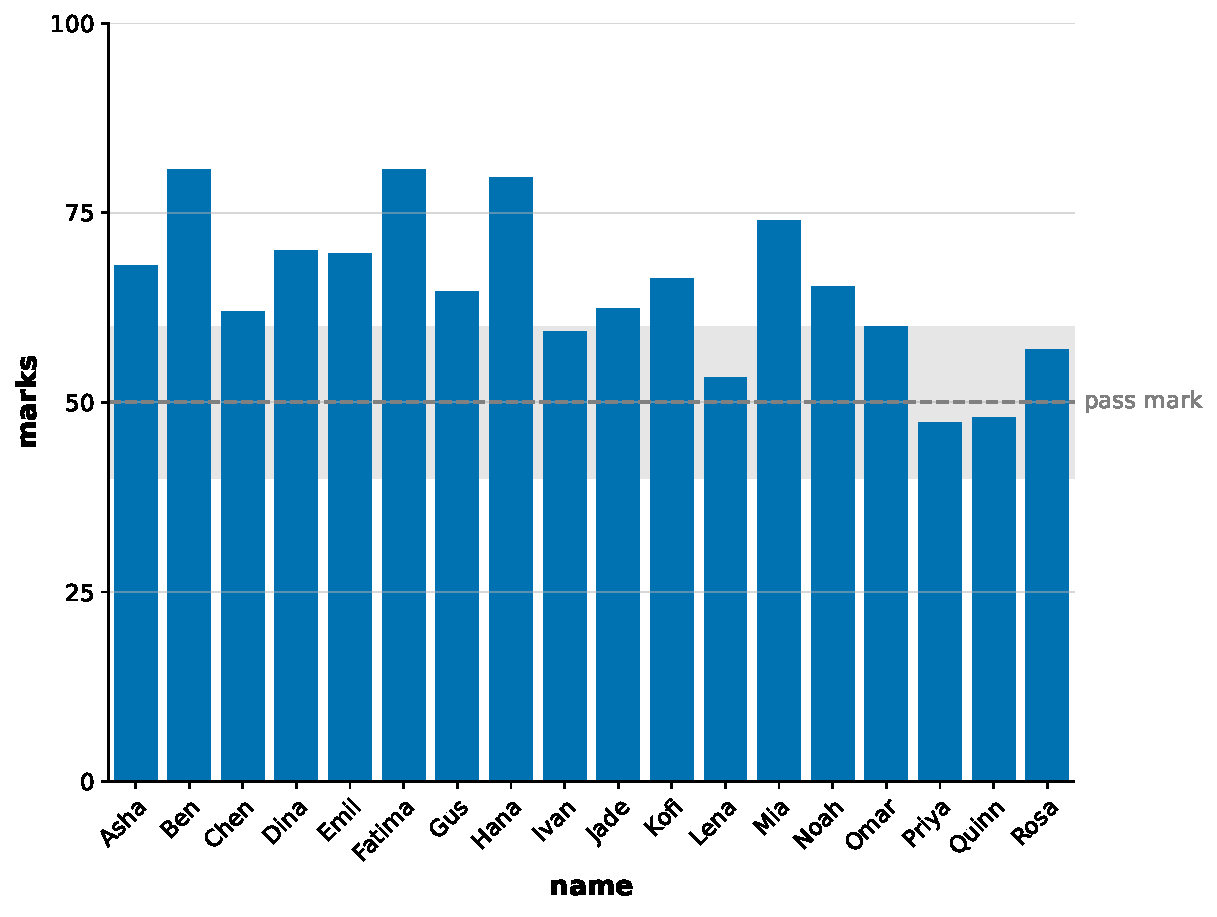
\includegraphics[width=0.72\textwidth,height=0.36\textheight,keepaspectratio]{figures/lesson06_example1_lesson6_marks.pdf}
\captionof{figure}{Lesson 6, example 1: \code{lesson6\_\allowbreak{}marks.\allowbreak{}png}.}
\end{minipage}\end{center}
\section*{Example 2}
On a log scale 1, 10, 100 and 1000 are the same distance apart. It helps when some numbers are much bigger than others.
\begin{lstlisting}[style=py]
import simplydata as sdata
growth = sdata.example("growth")
chart = sdata.chart(growth)
chart.lines(x="year", y="population", colour="country")
chart.log_scale_y()
chart.line_at_x(2010, label="2010")
chart.label_y("People (millions)")
chart.save("lesson6_log.png")
\end{lstlisting}
\whateachline
\begin{lineexplain}
  \item[1] Load simplydata.
  \item[2] Get the growth table: people in four made-up countries.
  \item[3] Start a chart.
  \item[4] One line per country.
  \item[5] Use a log scale on the y-axis. A country that grows by the same share each year now gets a straight line.
  \item[6] Draw an up-and-down line at the year 2010.
  \item[7] Name the y-axis.
  \item[8] Save it.
\end{lineexplain}
\printedoutput{output/lesson06_example2.txt}
\begin{center}\begin{minipage}{\linewidth}\centering
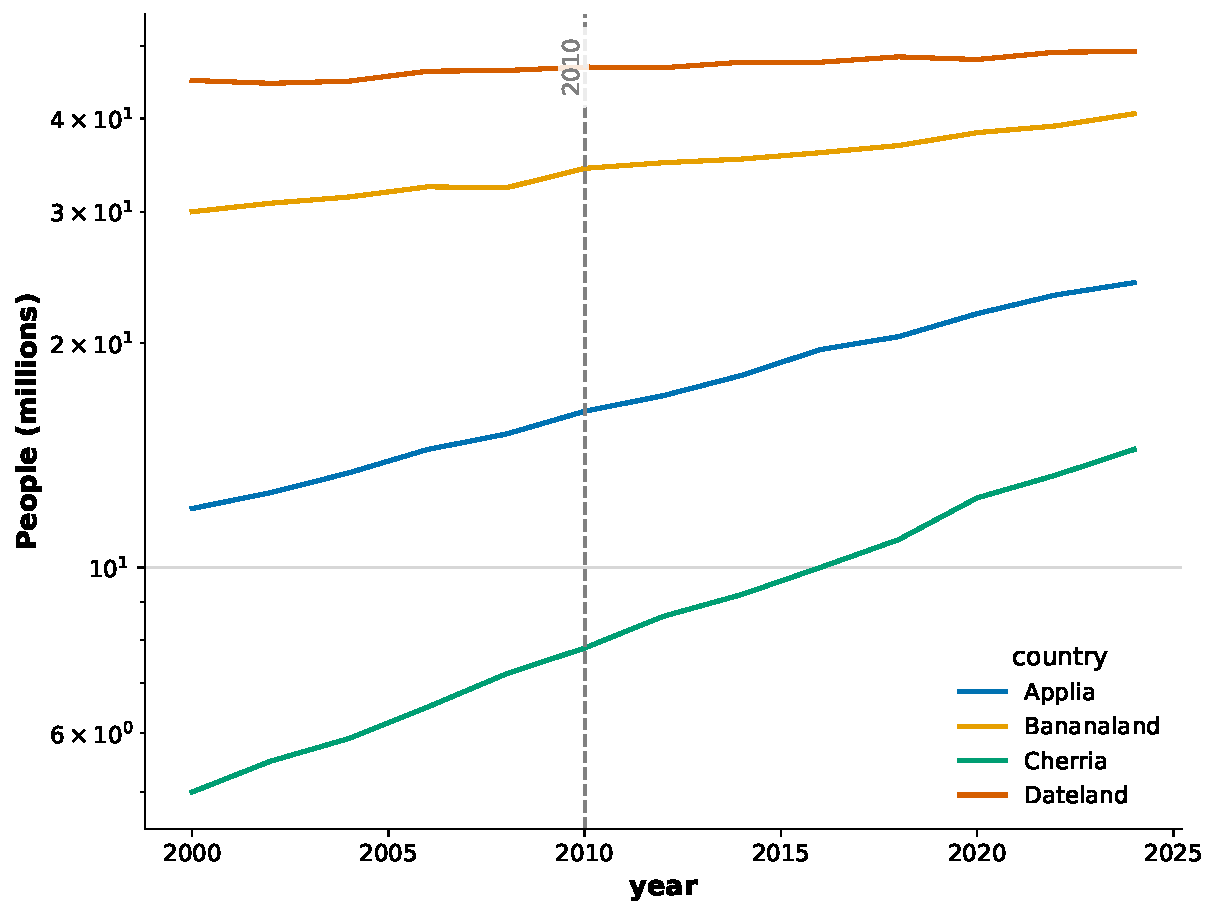
\includegraphics[width=0.72\textwidth,height=0.36\textheight,keepaspectratio]{figures/lesson06_example2_lesson6_log.pdf}
\captionof{figure}{Lesson 6, example 2: \code{lesson6\_\allowbreak{}log.\allowbreak{}png}.}
\end{minipage}\end{center}
\section*{Example 3}
A band shades the space between a low and a high value at each x: a range, or the uncertainty around a line.
\begin{lstlisting}[style=py]
import simplydata as sdata
days = {"day": [1, 2, 3, 4, 5], "lowest": [3, 5, 4, 6, 8], "average": [6, 8, 7, 9, 11], "highest": [9, 11, 10, 12, 14]}
chart = sdata.chart(days)
chart.band(x="day", between=["lowest", "highest"], label="lowest to highest")
chart.lines(x="day", y="average")
chart.label_y("Temperature (°C)")
chart.save("lesson6_band.png")
\end{lstlisting}
\whateachline
\begin{lineexplain}
  \item[1] Load simplydata.
  \item[2] A small table: the lowest, average and highest temperature on five days.
  \item[3] Start a chart of it.
  \item[4] Shade from the lowest to the highest value of each day. \code{label=} names it in the legend.
  \item[5] The average as a line through the band.
  \item[6] Name the y-axis.
  \item[7] Save it.
\end{lineexplain}
\printedoutput{output/lesson06_example3.txt}
\begin{center}\begin{minipage}{\linewidth}\centering
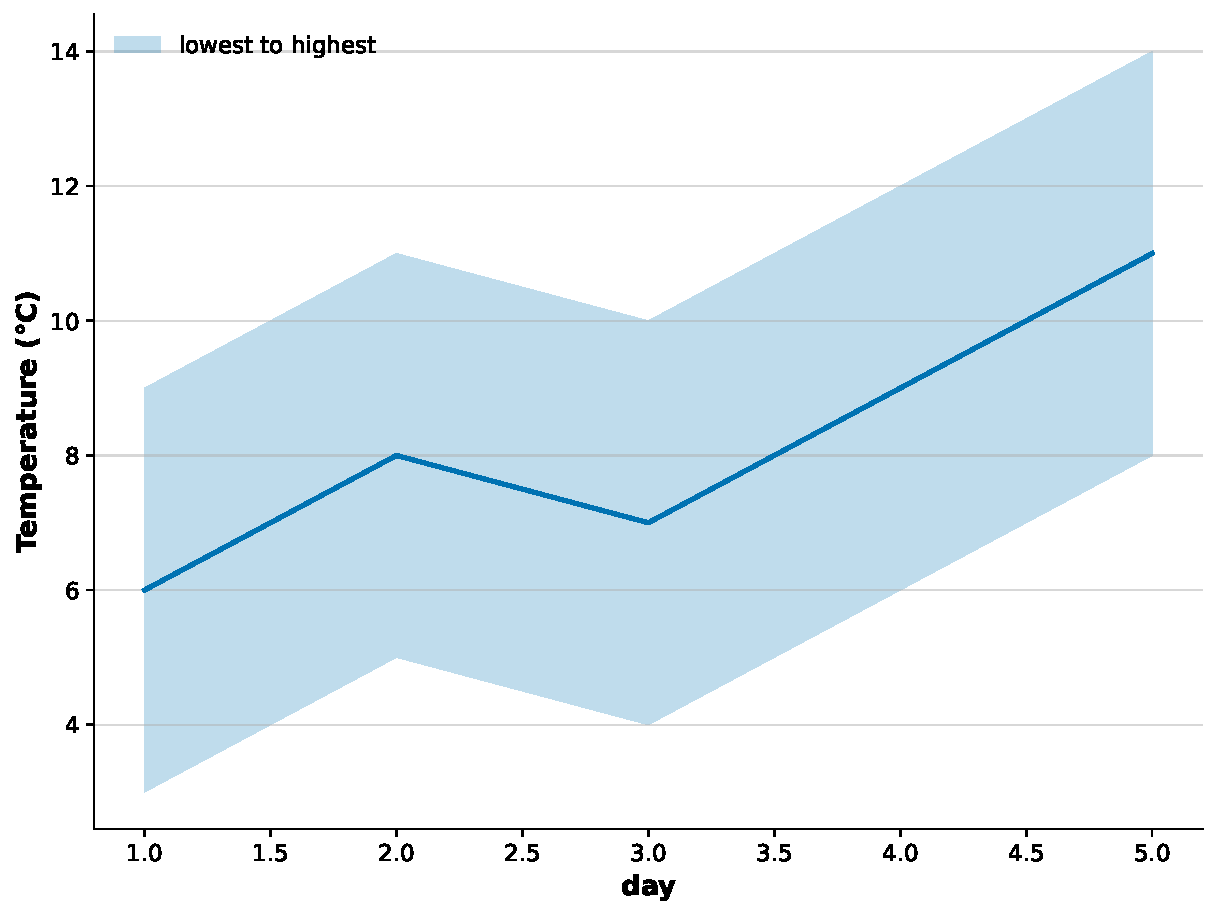
\includegraphics[width=0.72\textwidth,height=0.36\textheight,keepaspectratio]{figures/lesson06_example3_lesson6_band.pdf}
\captionof{figure}{Lesson 6, example 3: \code{lesson6\_\allowbreak{}band.\allowbreak{}png}.}
\end{minipage}\end{center}
\section*{Example 4}
Axes can say what their numbers mean, and a 1:1 line shows where two columns agree.
\begin{lstlisting}[style=py]
import simplydata as sdata
growth = sdata.example("growth")
chart = sdata.chart(growth)
chart.lines(x="year", y="forest", colour="country")
chart.tick_format_y("percent")
chart.save("lesson6_percent.png")
guesses = {"measured": [12, 18, 25, 31, 40], "predicted": [14, 17, 27, 29, 43]}
check = sdata.chart(guesses)
check.dots(x="measured", y="predicted")
check.line_with_slope(1, through=(0, 0), label="1:1")
check.save("lesson6_one_to_one.png")
\end{lstlisting}
\whateachline
\begin{lineexplain}
  \item[1] Load simplydata.
  \item[2] Get the growth table.
  \item[3] Start a chart.
  \item[4] The forest of each country, in \%.
  \item[5] Write the y numbers as 40 \%, 50 \% ... (\code{\textquotedbl{}thousands\textquotedbl{}}, \code{\textquotedbl{}scientific\textquotedbl{}} and dates such as \code{\textquotedbl{}Jan 2026\textquotedbl{}} work too).
  \item[6] Save it.
  \item[7] Five measured values and what a model predicted for them.
  \item[8] A second chart.
  \item[9] One dot per value.
  \item[10] The 1:1 line: dots on it were predicted exactly; above it, too high.
  \item[11] Save it.
\end{lineexplain}
\printedoutput{output/lesson06_example4.txt}
\begin{center}\begin{minipage}{\linewidth}\centering
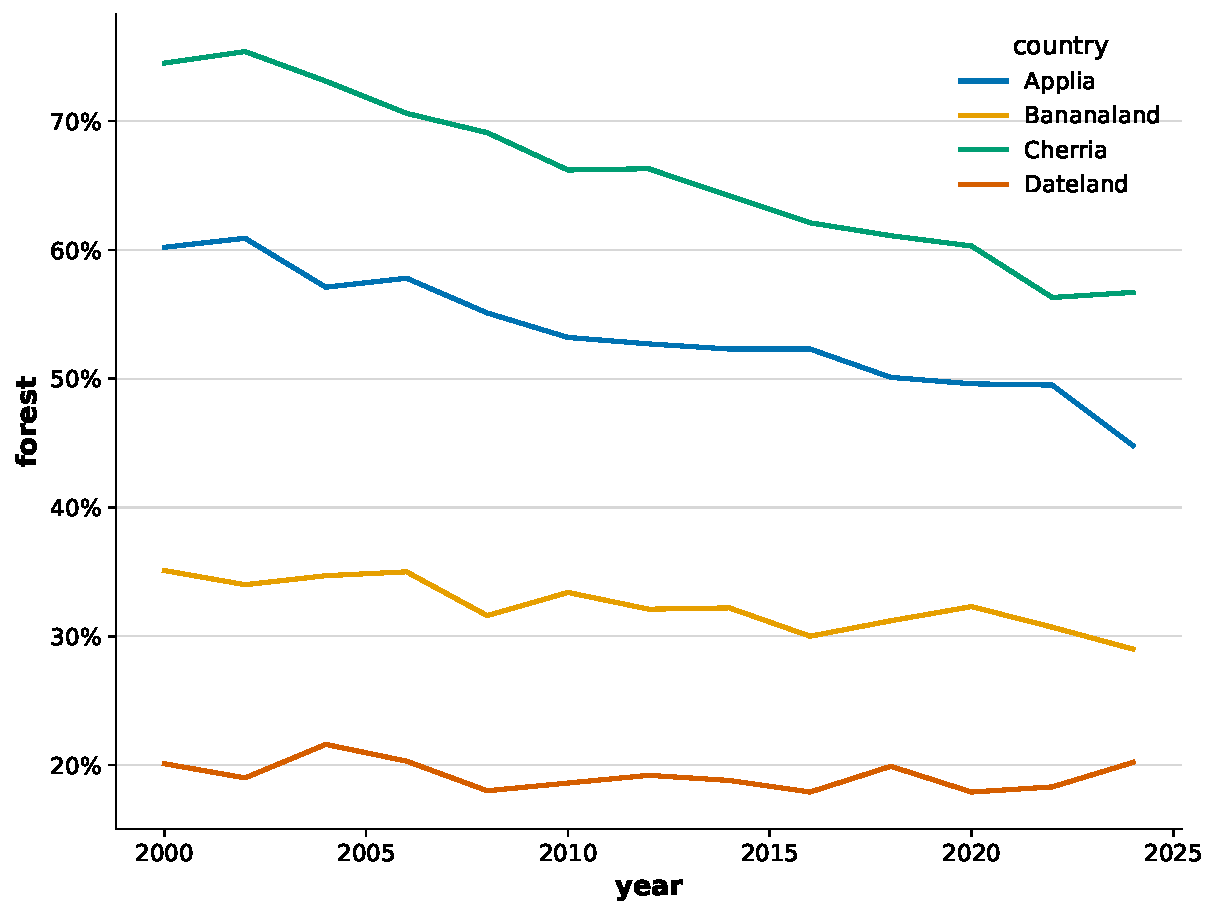
\includegraphics[width=0.48\textwidth,height=0.36\textheight,keepaspectratio]{figures/lesson06_example4_lesson6_percent.pdf}\hfill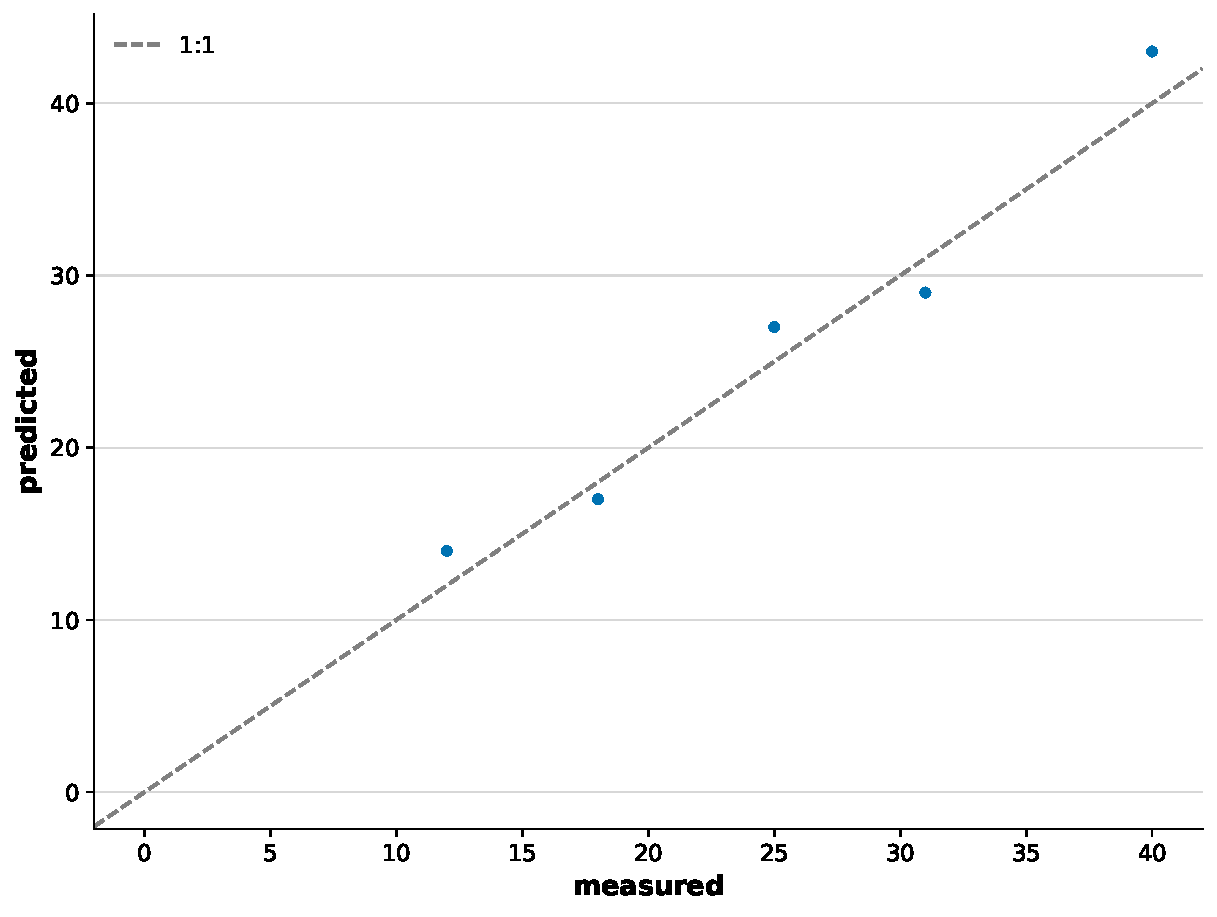
\includegraphics[width=0.48\textwidth,height=0.36\textheight,keepaspectratio]{figures/lesson06_example4_lesson6_one_to_one.pdf}
\captionof{figure}{Lesson 6, example 4: \code{lesson6\_\allowbreak{}percent.\allowbreak{}png} and \code{lesson6\_\allowbreak{}one\_\allowbreak{}to\_\allowbreak{}one.\allowbreak{}png}.}
\end{minipage}\end{center}
\begin{goodtoknow}
\begin{itemize}
  \item Every axis word ends in \_x or \_y: \code{range\_\allowbreak{}x}, \code{ticks\_\allowbreak{}x}, \code{log\_\allowbreak{}scale\_\allowbreak{}x}, \code{line\_\allowbreak{}at\_\allowbreak{}x}, \code{shade\_\allowbreak{}between\_\allowbreak{}x}, \code{flip\_\allowbreak{}x} ...
  \item \code{range\_\allowbreak{}y(0,\allowbreak{} None)} fixes only the bottom and lets the top choose itself.
  \item Bars should start at 0: a bar is read by its length, so a y-axis that starts at 40 makes small differences look big.
\end{itemize}
\end{goodtoknow}
\begin{tryit}
\begin{enumerate}
  \item Move the pass mark to 60 and shade between 0 and 40 instead.
  \item Take away \code{chart.\allowbreak{}log\_\allowbreak{}scale\_\allowbreak{}y()}. Which countries look different?
  \item Try \code{chart.\allowbreak{}flip\_\allowbreak{}y()} on any chart. What happens?
\end{enumerate}
Worked solutions: page~\pageref{solutions:6}, or type \code{sdata.\allowbreak{}lesson(6,\allowbreak{} solutions=True)}.
\end{tryit}
\par\noindent{\small\sffamily\textbf{Words in this lesson:} \hyperref[word:range-y]{\code{chart.\allowbreak{}range\_\allowbreak{}y()}}, \hyperref[word:ticks-y]{\code{chart.\allowbreak{}ticks\_\allowbreak{}y()}}, \hyperref[word:line-at-y]{\code{chart.\allowbreak{}line\_\allowbreak{}at\_\allowbreak{}y()}}, \hyperref[word:shade-between-y]{\code{chart.\allowbreak{}shade\_\allowbreak{}between\_\allowbreak{}y()}}, \hyperref[word:log-scale-y]{\code{chart.\allowbreak{}log\_\allowbreak{}scale\_\allowbreak{}y()}}, \hyperref[word:line-at-x]{\code{chart.\allowbreak{}line\_\allowbreak{}at\_\allowbreak{}x()}}, \hyperref[word:flip-y]{\code{chart.\allowbreak{}flip\_\allowbreak{}y()}}, \hyperref[word:band]{\code{chart.\allowbreak{}band()}}, \hyperref[word:tick-format-y]{\code{chart.\allowbreak{}tick\_\allowbreak{}format\_\allowbreak{}y()}}, \hyperref[word:line-with-slope]{\code{chart.\allowbreak{}line\_\allowbreak{}with\_\allowbreak{}slope()}}.\par}

\chapter{Several charts together}\label{lesson:7}
\begin{learnbox}
\begin{itemize}
  \item how to make one small chart for each group
  \item how to put different charts on one page: side by side, one above the other, or in a grid
  \item how to write A, B, C on the charts, as figures in papers have
  \item how to compare every number column with every other
\end{itemize}
\end{learnbox}
\section*{Example 1}
\code{one\_\allowbreak{}chart\_\allowbreak{}per} draws the same chart once for each group.
\begin{lstlisting}[style=py]
import simplydata as sdata
marks = sdata.example("marks")
chart = sdata.chart(marks)
chart.dots(x="hours", y="marks")
chart.fit_line()
chart.one_chart_per("class")
chart.save("lesson7_one_chart_per.png")
\end{lstlisting}
\whateachline
\begin{lineexplain}
  \item[1] Load simplydata.
  \item[2] Get the marks table.
  \item[3] Start a chart.
  \item[4] Dots of hours and marks.
  \item[5] Add a fit line.
  \item[6] Make one small chart for each class, with the same axes so they are easy to compare.
  \item[7] Save it.
\end{lineexplain}
\printedoutput{output/lesson07_example1.txt}
\begin{center}\begin{minipage}{\linewidth}\centering
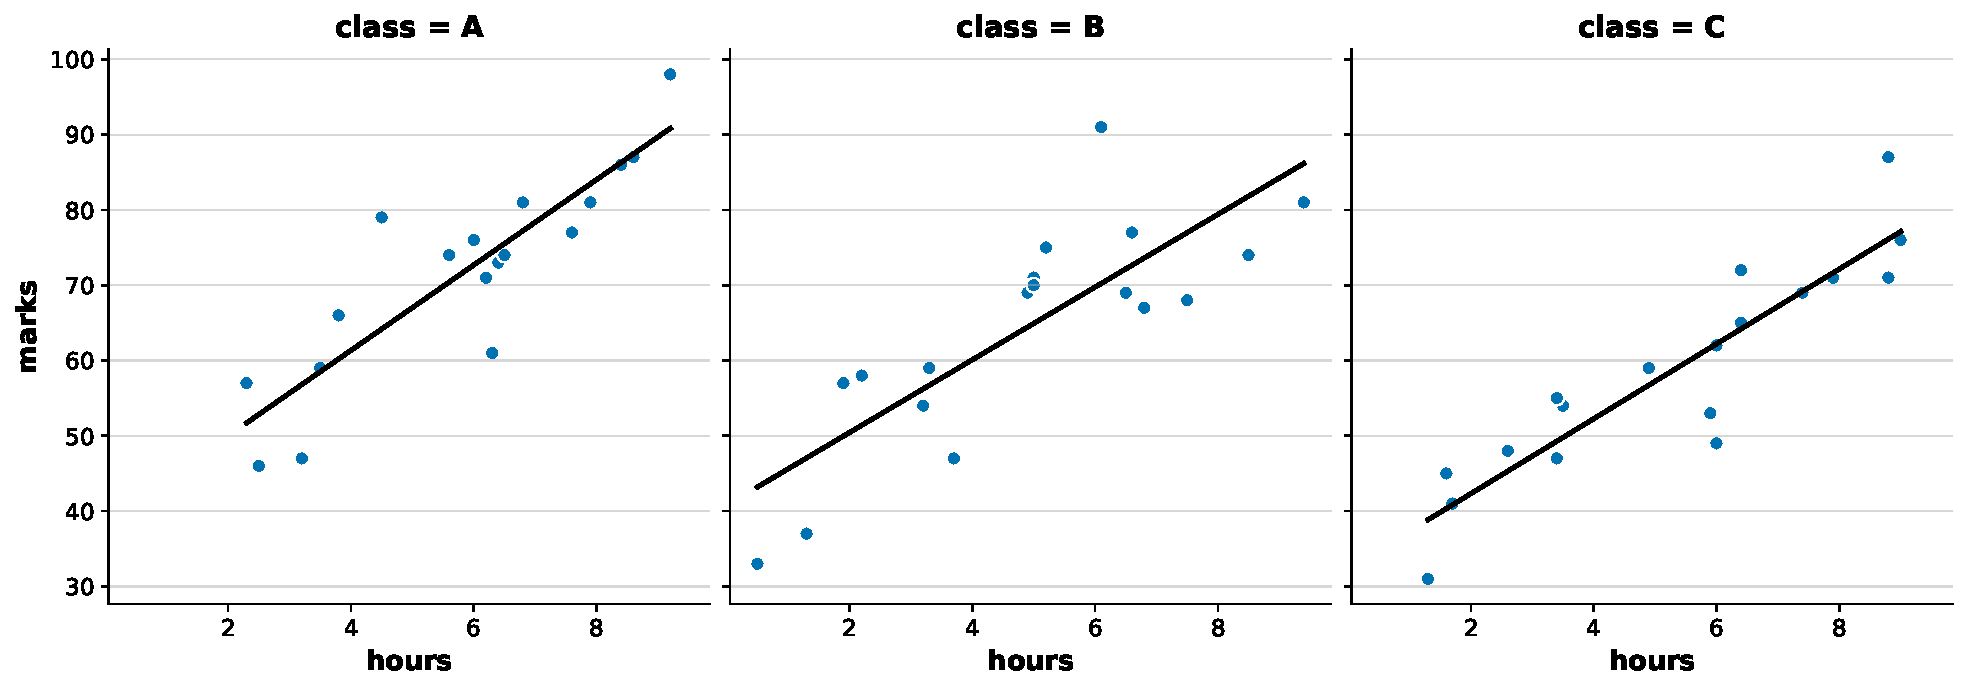
\includegraphics[width=0.72\textwidth,height=0.36\textheight,keepaspectratio]{figures/lesson07_example1_lesson7_one_chart_per.pdf}
\captionof{figure}{Lesson 7, example 1: \code{lesson7\_\allowbreak{}one\_\allowbreak{}chart\_\allowbreak{}per.\allowbreak{}png}.}
\end{minipage}\end{center}
\section*{Example 2}
Each chart is an object of its own, so different charts can share one page.
\begin{lstlisting}[style=py]
import simplydata as sdata
weather = sdata.example("weather")
a = sdata.chart(weather).lines(x="month", y="temperature", colour="city")
b = sdata.chart(weather).bars(x="month", y="rain", colour="city")
page = sdata.one_above_other(a, b)
page.title_top("A year of weather")
page.save("lesson7_page.png")
\end{lstlisting}
\whateachline
\begin{lineexplain}
  \item[1] Load simplydata.
  \item[2] Get the weather table.
  \item[3] Make a first chart, called a. Steps can also be joined with dots on one line.
  \item[4] Make a second chart, called b.
  \item[5] Put a above b on one page.
  \item[6] Give the whole page a title.
  \item[7] Save the page.
\end{lineexplain}
\printedoutput{output/lesson07_example2.txt}
\begin{center}\begin{minipage}{\linewidth}\centering
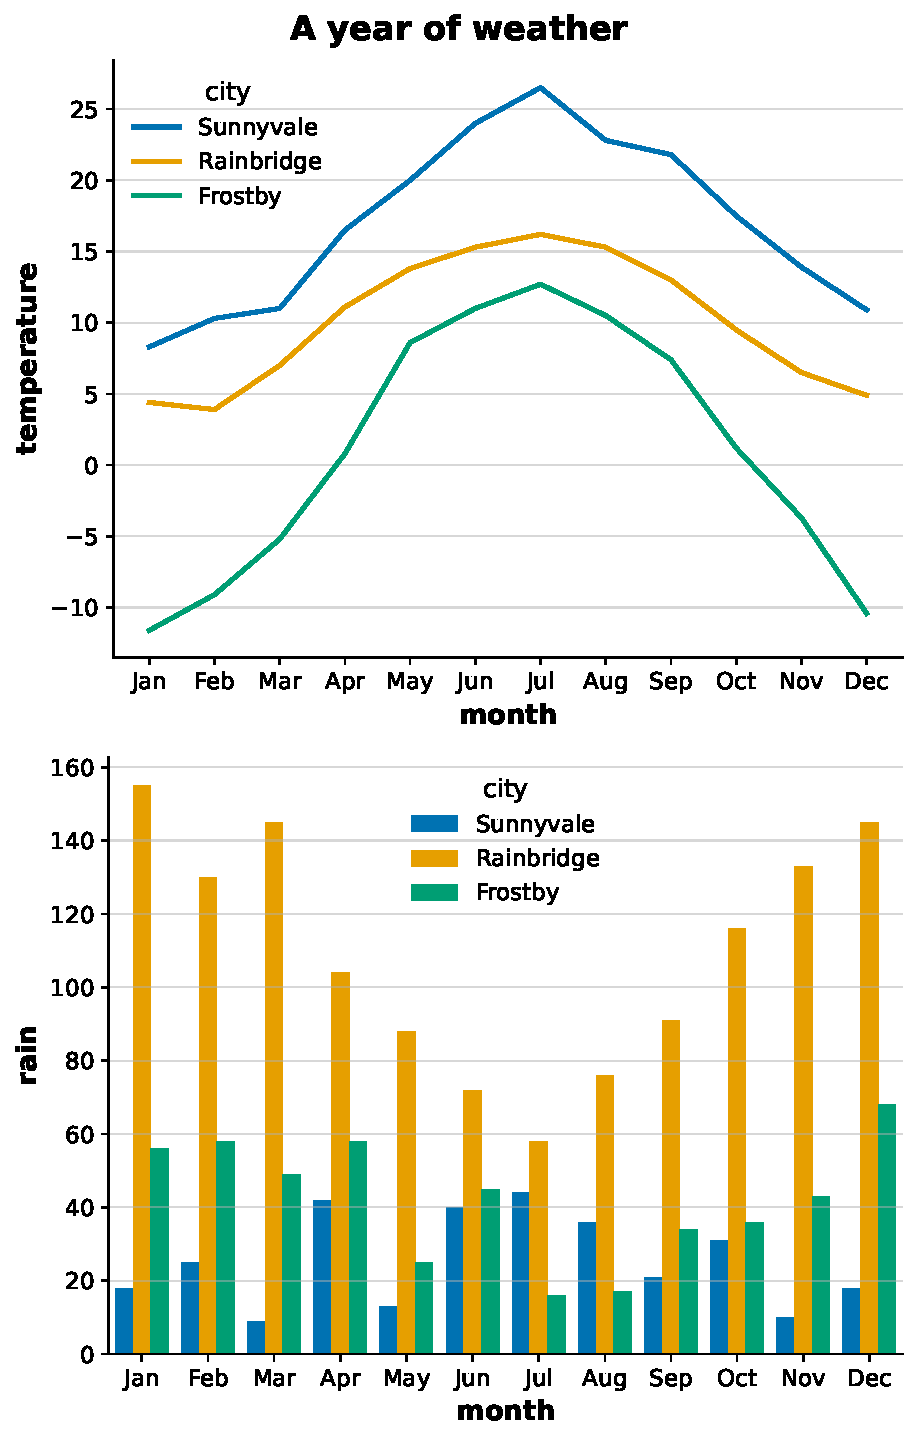
\includegraphics[width=0.72\textwidth,height=0.36\textheight,keepaspectratio]{figures/lesson07_example2_lesson7_page.pdf}
\captionof{figure}{Lesson 7, example 2: \code{lesson7\_\allowbreak{}page.\allowbreak{}png}.}
\end{minipage}\end{center}
\section*{Example 3}
A grid holds many charts in rows and columns. \code{letters=True} writes A, B, C and D on them, as figures in papers have.
\begin{lstlisting}[style=py]
import simplydata as sdata
marks = sdata.example("marks")
a = sdata.chart(marks).bars(x="class", y="marks").title_top("Average")
b = sdata.chart(marks).histogram(x="marks").title_top("All marks")
c = sdata.chart(marks).dots(x="height", y="marks").title_top("Height")
d = sdata.chart(marks).boxes(x="subject", y="marks").title_top("Subjects")
page = sdata.grid(a, b, c, d, per_row=2, letters=True)
page.save("lesson7_grid.png")
\end{lstlisting}
\whateachline
\begin{lineexplain}
  \item[1] Load simplydata.
  \item[2] Get the marks table.
  \item[3] Chart a.
  \item[4] Chart b.
  \item[5] Chart c.
  \item[6] Chart d.
  \item[7] All four in a grid, 2 charts per row, with a letter on each.
  \item[8] Save it.
\end{lineexplain}
\printedoutput{output/lesson07_example3.txt}
\begin{center}\begin{minipage}{\linewidth}\centering
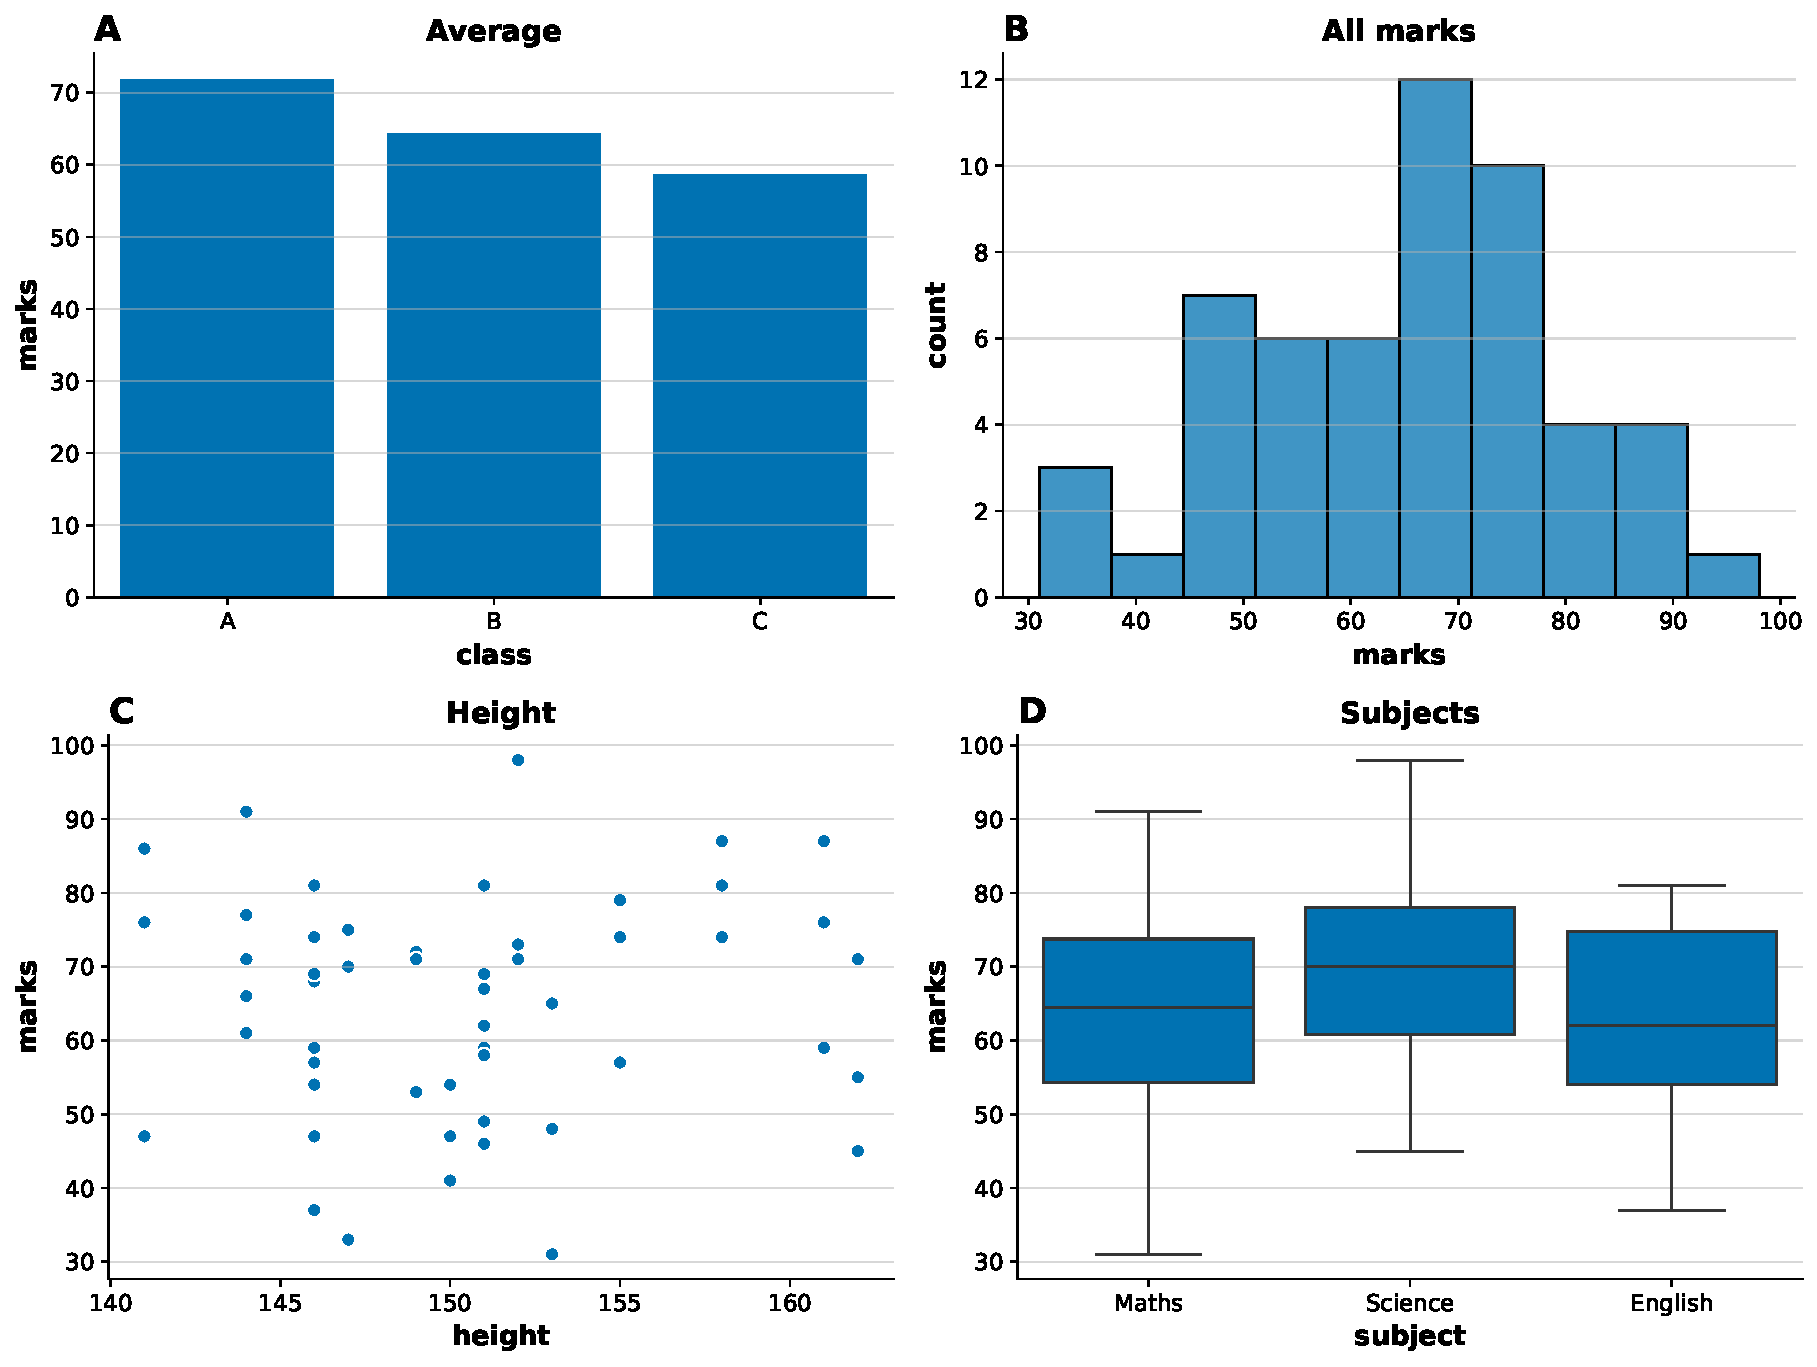
\includegraphics[width=0.72\textwidth,height=0.36\textheight,keepaspectratio]{figures/lesson07_example3_lesson7_grid.pdf}
\captionof{figure}{Lesson 7, example 3: \code{lesson7\_\allowbreak{}grid.\allowbreak{}png}.}
\end{minipage}\end{center}
\section*{Example 4}
Charts from different tables can share a page too.
\begin{lstlisting}[style=py]
import simplydata as sdata
rain = sdata.chart(sdata.example("weather")).lines(x="month", y="rain", colour="city")
forest = sdata.chart(sdata.example("growth")).lines(x="year", y="forest", colour="country")
page = sdata.side_by_side(rain, forest, letters=True)
page.save("lesson7_two_tables.png")
\end{lstlisting}
\whateachline
\begin{lineexplain}
  \item[1] Load simplydata.
  \item[2] A chart of the weather table, called rain.
  \item[3] A chart of the growth table, called forest.
  \item[4] Put the two charts next to each other, with A and B.
  \item[5] Save the page.
\end{lineexplain}
\printedoutput{output/lesson07_example4.txt}
\begin{center}\begin{minipage}{\linewidth}\centering
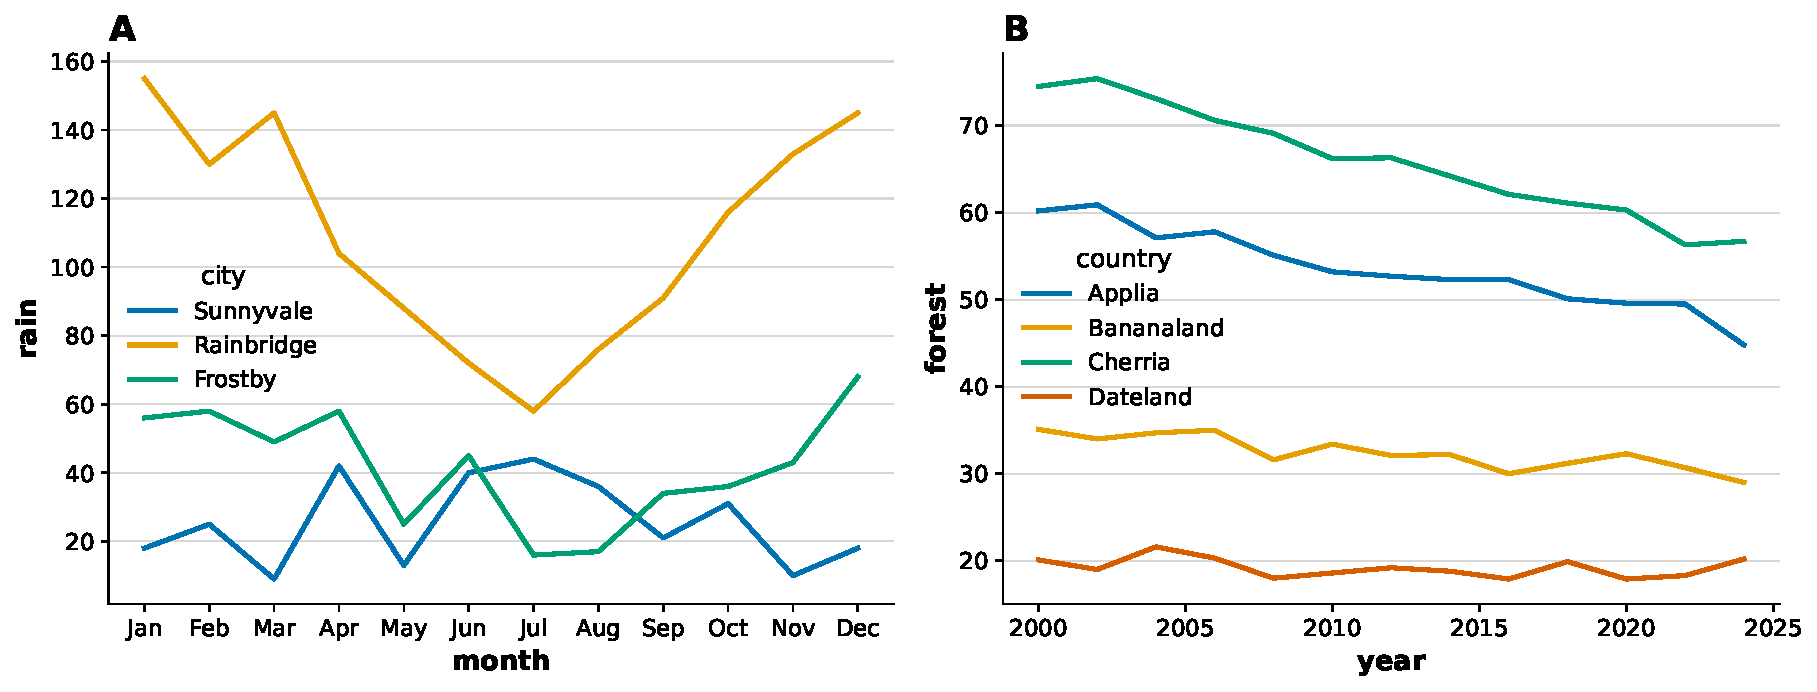
\includegraphics[width=0.72\textwidth,height=0.36\textheight,keepaspectratio]{figures/lesson07_example4_lesson7_two_tables.pdf}
\captionof{figure}{Lesson 7, example 4: \code{lesson7\_\allowbreak{}two\_\allowbreak{}tables.\allowbreak{}png}.}
\end{minipage}\end{center}
\section*{Example 5}
\code{sdata.\allowbreak{}pairs} draws every number column against every other, in one go.
\begin{lstlisting}[style=py]
import simplydata as sdata
pairs = sdata.pairs(sdata.example("marks"), colour="class")
pairs.save("lesson7_pairs.png")
\end{lstlisting}
\whateachline
\begin{lineexplain}
  \item[1] Load simplydata.
  \item[2] Hours, marks and height, each against each other. The middle line shows how each column is spread out.
  \item[3] Save it. Which two columns go together?
\end{lineexplain}
\printedoutput{output/lesson07_example5.txt}
\begin{center}\begin{minipage}{\linewidth}\centering
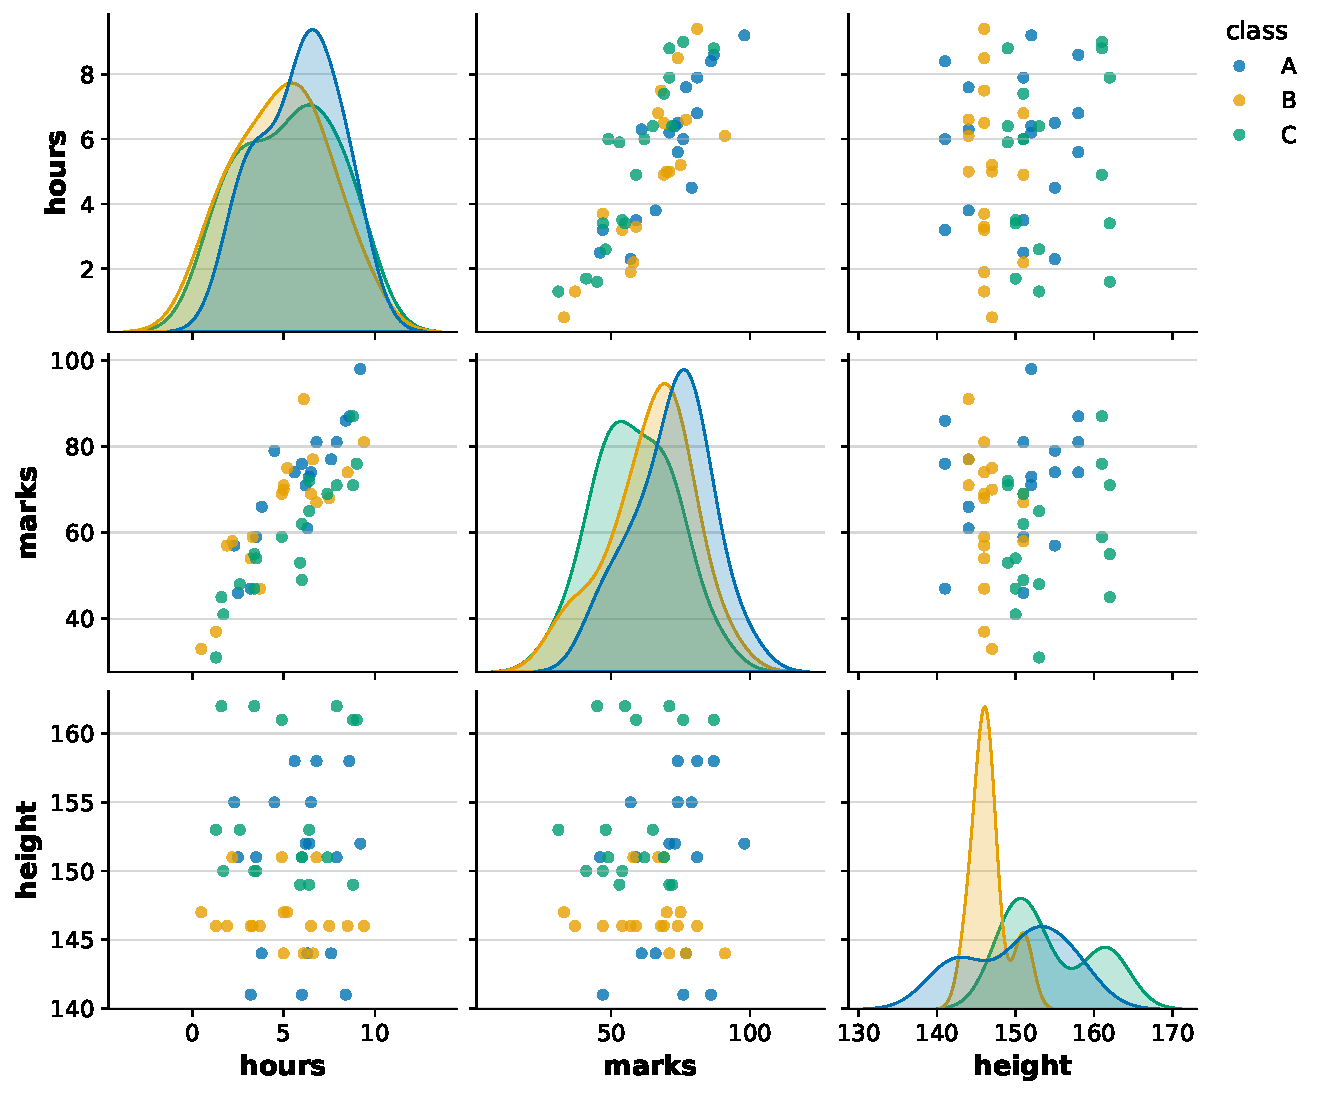
\includegraphics[width=0.72\textwidth,height=0.36\textheight,keepaspectratio]{figures/lesson07_example5_lesson7_pairs.pdf}
\captionof{figure}{Lesson 7, example 5: \code{lesson7\_\allowbreak{}pairs.\allowbreak{}png}.}
\end{minipage}\end{center}
\begin{goodtoknow}
\begin{itemize}
  \item \code{same\_\allowbreak{}y=True} gives all the charts on a page the same y-axis, so heights can be compared fairly: \code{sdata.\allowbreak{}side\_\allowbreak{}by\_\allowbreak{}side(a,\allowbreak{} b,\allowbreak{} same\_\allowbreak{}y=True)}.
  \item \code{sdata.\allowbreak{}side\_\allowbreak{}by\_\allowbreak{}side}, \code{sdata.\allowbreak{}one\_\allowbreak{}above\_\allowbreak{}other} and \code{sdata.\allowbreak{}grid} all take \code{letters=True}.
  \item \code{chart.\allowbreak{}one\_\allowbreak{}chart\_\allowbreak{}per(down=\textquotedbl{}class\textquotedbl{},\allowbreak{} across=\textquotedbl{}subject\textquotedbl{})} makes a table of small charts: the classes go down, the subjects go across. \code{per\_\allowbreak{}row=3} puts 3 small charts in a row.
\end{itemize}
\end{goodtoknow}
\begin{tryit}
\begin{enumerate}
  \item Change \code{chart.\allowbreak{}one\_\allowbreak{}chart\_\allowbreak{}per(\textquotedbl{}class\textquotedbl{})} to \code{chart.\allowbreak{}one\_\allowbreak{}chart\_\allowbreak{}per(\textquotedbl{}subject\textquotedbl{})}.
  \item Use \code{sdata.\allowbreak{}side\_\allowbreak{}by\_\allowbreak{}side(a,\allowbreak{} b)} instead of \code{sdata.\allowbreak{}one\_\allowbreak{}above\_\allowbreak{}other(a,\allowbreak{} b)} for the weather charts.
  \item Make \code{sdata.\allowbreak{}pairs} of \code{sdata.\allowbreak{}example(\textquotedbl{}weather\textquotedbl{})} with \code{colour=\textquotedbl{}city\textquotedbl{}}.
\end{enumerate}
Worked solutions: page~\pageref{solutions:7}, or type \code{sdata.\allowbreak{}lesson(7,\allowbreak{} solutions=True)}.
\end{tryit}
\par\noindent{\small\sffamily\textbf{Words in this lesson:} \hyperref[word:one-chart-per]{\code{chart.\allowbreak{}one\_\allowbreak{}chart\_\allowbreak{}per()}}, \hyperref[word:sdata.one-above-other]{\code{sdata.\allowbreak{}one\_\allowbreak{}above\_\allowbreak{}other()}}, \hyperref[word:sdata.grid]{\code{sdata.\allowbreak{}grid()}}, \hyperref[word:sdata.side-by-side]{\code{sdata.\allowbreak{}side\_\allowbreak{}by\_\allowbreak{}side()}}, \hyperref[word:sdata.pairs]{\code{sdata.\allowbreak{}pairs()}}, \hyperref[word:fit-line]{\code{chart.\allowbreak{}fit\_\allowbreak{}line()}}, \hyperref[word:histogram]{\code{chart.\allowbreak{}histogram()}}.\par}

\chapter{Hard tricks, and your own program}\label{lesson:8}
\begin{learnbox}
\begin{itemize}
  \item a second y-axis, a zoom box and a moving chart
  \item a heatmap that sorts itself
  \item how to write your own program from start to end
\end{itemize}
\end{learnbox}
\section*{Example 1}
A second y-axis shows a column measured in other units on the same chart.
\begin{lstlisting}[style=py]
import simplydata as sdata
weather = sdata.example("weather")
chart = sdata.chart(weather)
chart.lines(x="month", y="temperature")
chart.second_y("rain", drawn_as="bars", label="Rain (mm)")
chart.label_y("Temperature (°C)")
chart.save("lesson8_second_y.png")
\end{lstlisting}
\whateachline
\begin{lineexplain}
  \item[1] Load simplydata.
  \item[2] Get the weather table.
  \item[3] Start a chart.
  \item[4] A line of temperature (average of the three cities).
  \item[5] Add rain, drawn as bars, with its own y-axis on the right.
  \item[6] Name the left y-axis.
  \item[7] Save it.
\end{lineexplain}
\printedoutput{output/lesson08_example1.txt}
\begin{center}\begin{minipage}{\linewidth}\centering
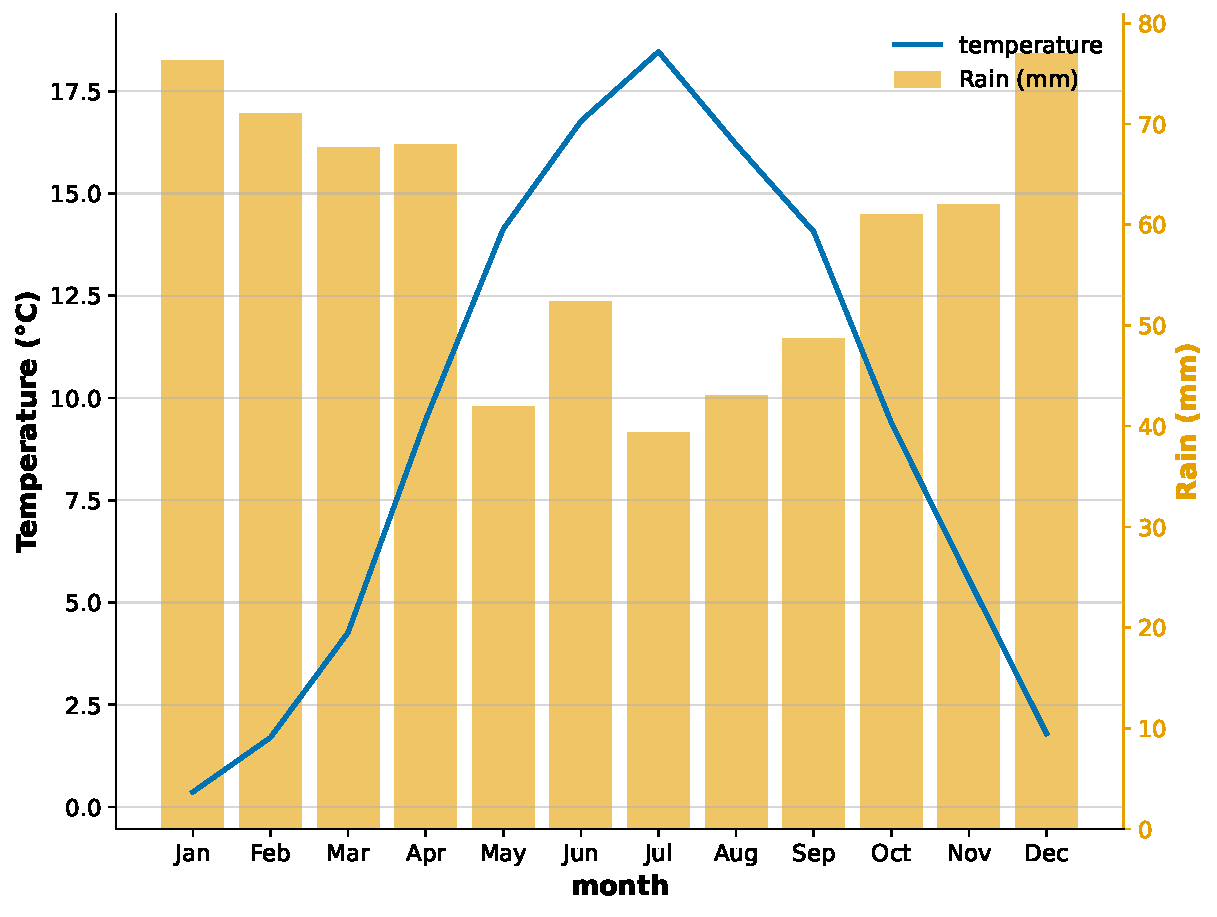
\includegraphics[width=0.72\textwidth,height=0.36\textheight,keepaspectratio]{figures/lesson08_example1_lesson8_second_y.pdf}
\captionof{figure}{Lesson 8, example 1: \code{lesson8\_\allowbreak{}second\_\allowbreak{}y.\allowbreak{}png}.}
\end{minipage}\end{center}
\section*{Example 2}
A zoom box shows a small part of the chart close up.
\begin{lstlisting}[style=py]
import simplydata as sdata
marks = sdata.example("marks")
chart = sdata.chart(marks)
chart.dots(x="hours", y="marks")
chart.zoom_box(x_between=[2, 4], y_between=[40, 60], where="top left")
chart.save("lesson8_zoom.png")
\end{lstlisting}
\whateachline
\begin{lineexplain}
  \item[1] Load simplydata.
  \item[2] Get the marks table.
  \item[3] Start a chart.
  \item[4] Dots of hours and marks.
  \item[5] Show the part between 2 and 4 hours and between 40 and 60 marks, bigger, in a box at the top left.
  \item[6] Save it.
\end{lineexplain}
\printedoutput{output/lesson08_example2.txt}
\begin{center}\begin{minipage}{\linewidth}\centering
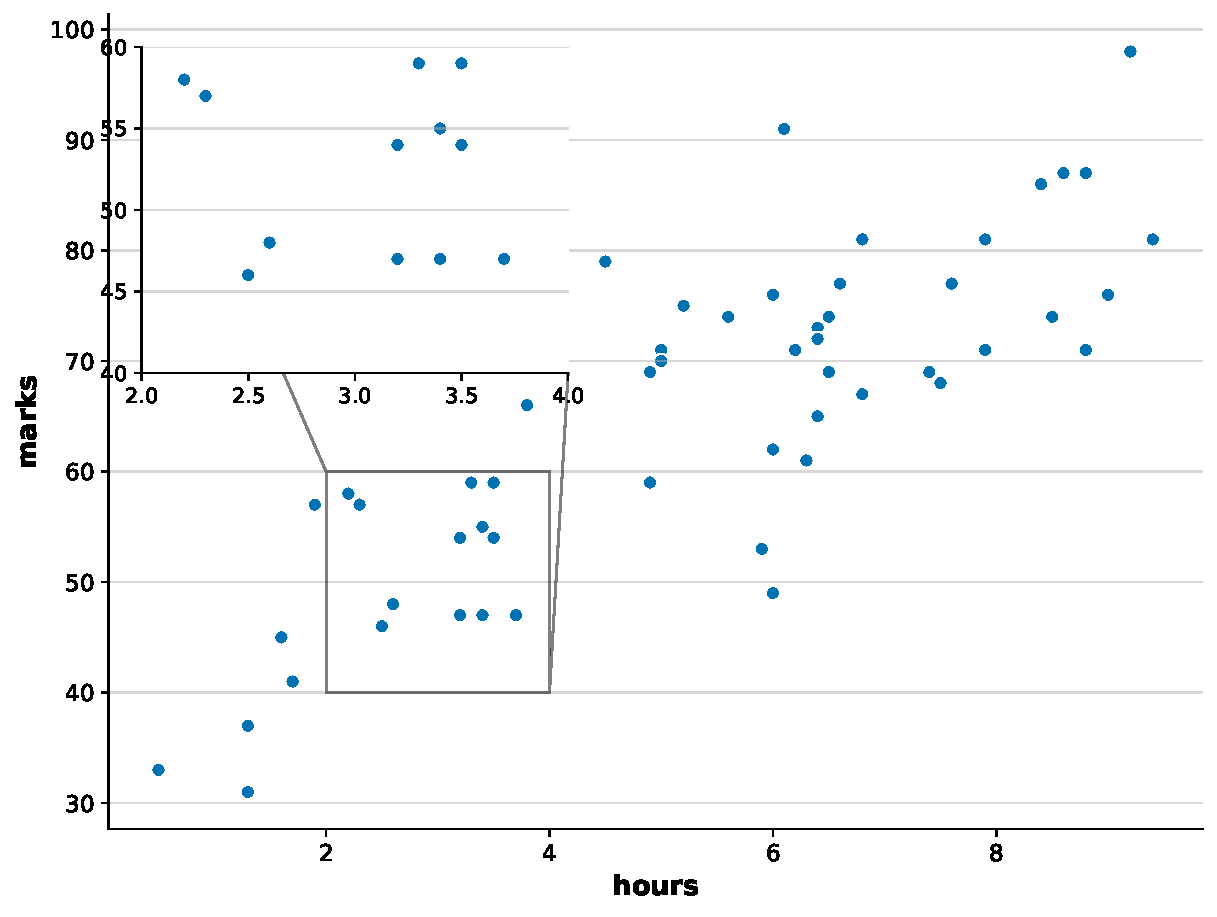
\includegraphics[width=0.72\textwidth,height=0.36\textheight,keepaspectratio]{figures/lesson08_example2_lesson8_zoom.pdf}
\captionof{figure}{Lesson 8, example 2: \code{lesson8\_\allowbreak{}zoom.\allowbreak{}png}.}
\end{minipage}\end{center}
\section*{Example 3}
A heatmap colours a grid of numbers. \code{cluster=True} puts rows that are alike next to each other.
\begin{lstlisting}[style=py]
import simplydata as sdata
weather = sdata.example("weather")
chart = sdata.chart(weather)
chart.heatmap(x="month", y="city", value="rain", numbers=True, cluster=True)
chart.label_colour_bar("Rain (mm)")
chart.size(width=12, height=4)
chart.save("lesson8_heatmap.png")
\end{lstlisting}
\whateachline
\begin{lineexplain}
  \item[1] Load simplydata.
  \item[2] Get the weather table.
  \item[3] Start a chart.
  \item[4] One square per city and month, coloured by rain, with the number written in. \code{cluster=True} sorts the rows and columns and draws a tree of how alike they are (hierarchical clustering).
  \item[5] Name the colour bar.
  \item[6] Make the chart wide and low.
  \item[7] Save it.
\end{lineexplain}
\printedoutput{output/lesson08_example3.txt}
\begin{center}\begin{minipage}{\linewidth}\centering
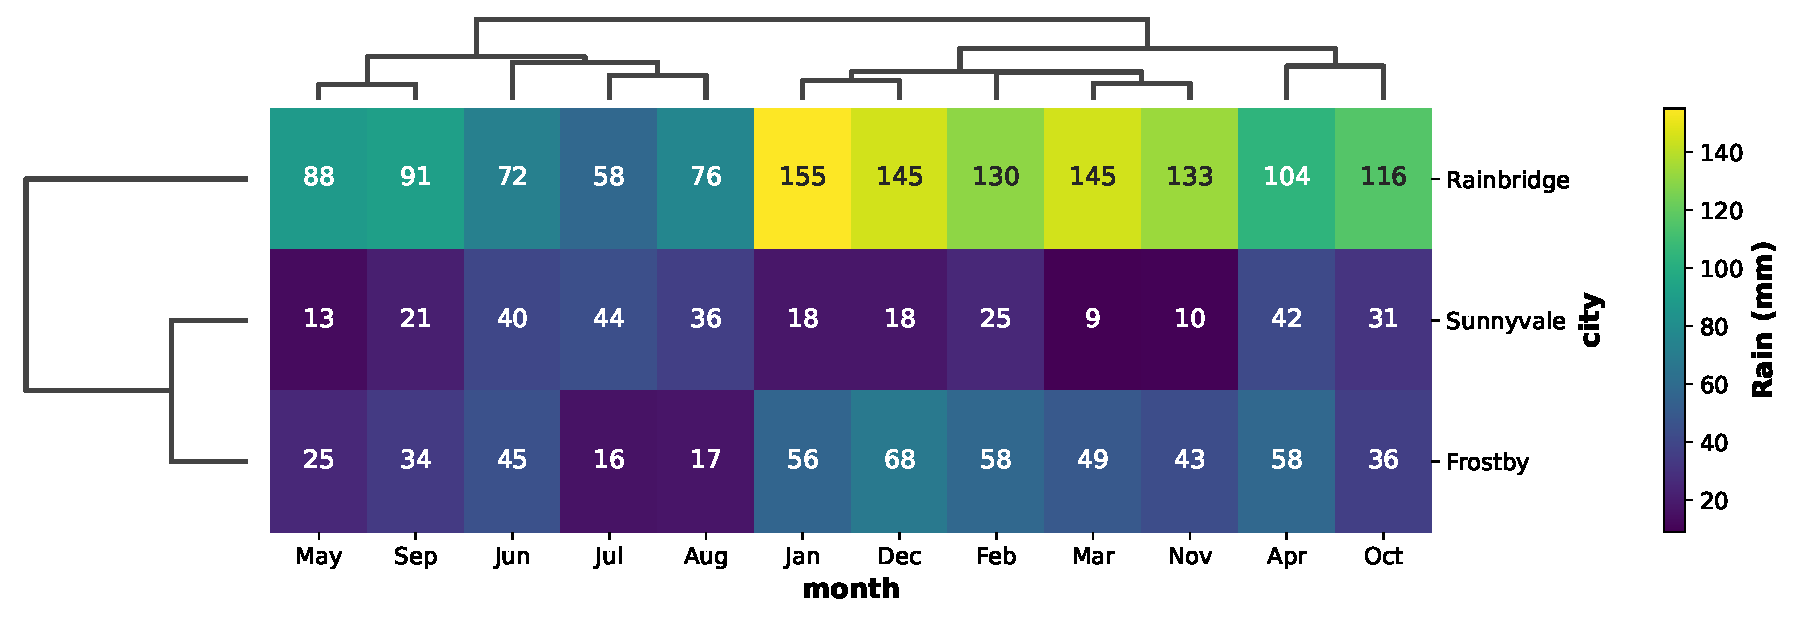
\includegraphics[width=0.72\textwidth,height=0.36\textheight,keepaspectratio]{figures/lesson08_example3_lesson8_heatmap.pdf}
\captionof{figure}{Lesson 8, example 3: \code{lesson8\_\allowbreak{}heatmap.\allowbreak{}png}.}
\end{minipage}\end{center}
\section*{Example 4}
An animation is a chart that moves: one picture for each value of a column.
\begin{lstlisting}[style=py]
import simplydata as sdata
growth = sdata.example("growth")
chart = sdata.chart(growth)
chart.bars(x="country", y="population")
chart.range_y(0, 50)
chart.animate(over="year")
chart.save("lesson8_growth.gif")
\end{lstlisting}
\whateachline
\begin{lineexplain}
  \item[1] Load simplydata.
  \item[2] Get the growth table.
  \item[3] Start a chart.
  \item[4] One bar per country.
  \item[5] Keep the y-axis still, from 0 to 50.
  \item[6] Make one picture for each year.
  \item[7] Save it as a \code{.\allowbreak{}gif}, a moving picture. Open it in a web browser to watch.
\end{lineexplain}
\printedoutput{output/lesson08_example4.txt}
\begin{center}\begin{minipage}{\linewidth}\centering
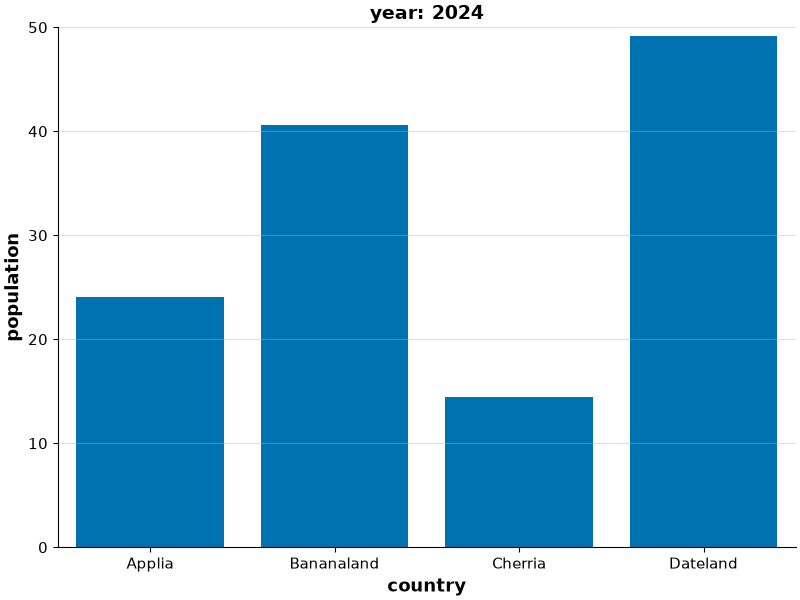
\includegraphics[width=0.72\textwidth,height=0.36\textheight,keepaspectratio]{figures/lesson08_example4_lesson8_growth.png}
\captionof{figure}{Lesson 8, example 4: \code{lesson8\_\allowbreak{}growth.\allowbreak{}gif} (the last picture of the animation).}
\end{minipage}\end{center}
\section*{Example 5}
Your own program. Every chart follows the same plan: get the data, look, start, draw, words, look, save.
\begin{lstlisting}[style=py]
import simplydata as sdata
island = sdata.example("island")
print(island)
chart = sdata.chart(island)
chart.contour(x="east", y="north", z="height")
chart.title_top("Treasure Island")
chart.label_x("East (km)")
chart.label_y("North (km)")
chart.label_colour_bar("Height (m)")
chart.note("X marks the spot", x=10, y=4, arrow=True)
chart.style("presentation")
chart.save("lesson8_my_program.png")
\end{lstlisting}
\whateachline
\begin{lineexplain}
  \item[1] 1. Load simplydata.
  \item[2] 2. Get the data. For your own file, skip this line and write chart = \code{sdata.\allowbreak{}chart(\textquotedbl{}my\_\allowbreak{}file.\allowbreak{}xlsx\textquotedbl{})} below.
  \item[3] 3. Look at the data before you draw it.
  \item[4] 4. Start a chart.
  \item[5] 5. Draw: a map where each colour band is one height.
  \item[6] 6. Words: a title ...
  \item[7] ... and the axis names ...
  \item[9] ... and the name of the colour bar.
  \item[10] A note with an arrow.
  \item[11] 7. Look: big and clear for showing to others.
  \item[12] 8. Save.
\end{lineexplain}
\printedoutput{output/lesson08_example5.txt}
\begin{center}\begin{minipage}{\linewidth}\centering
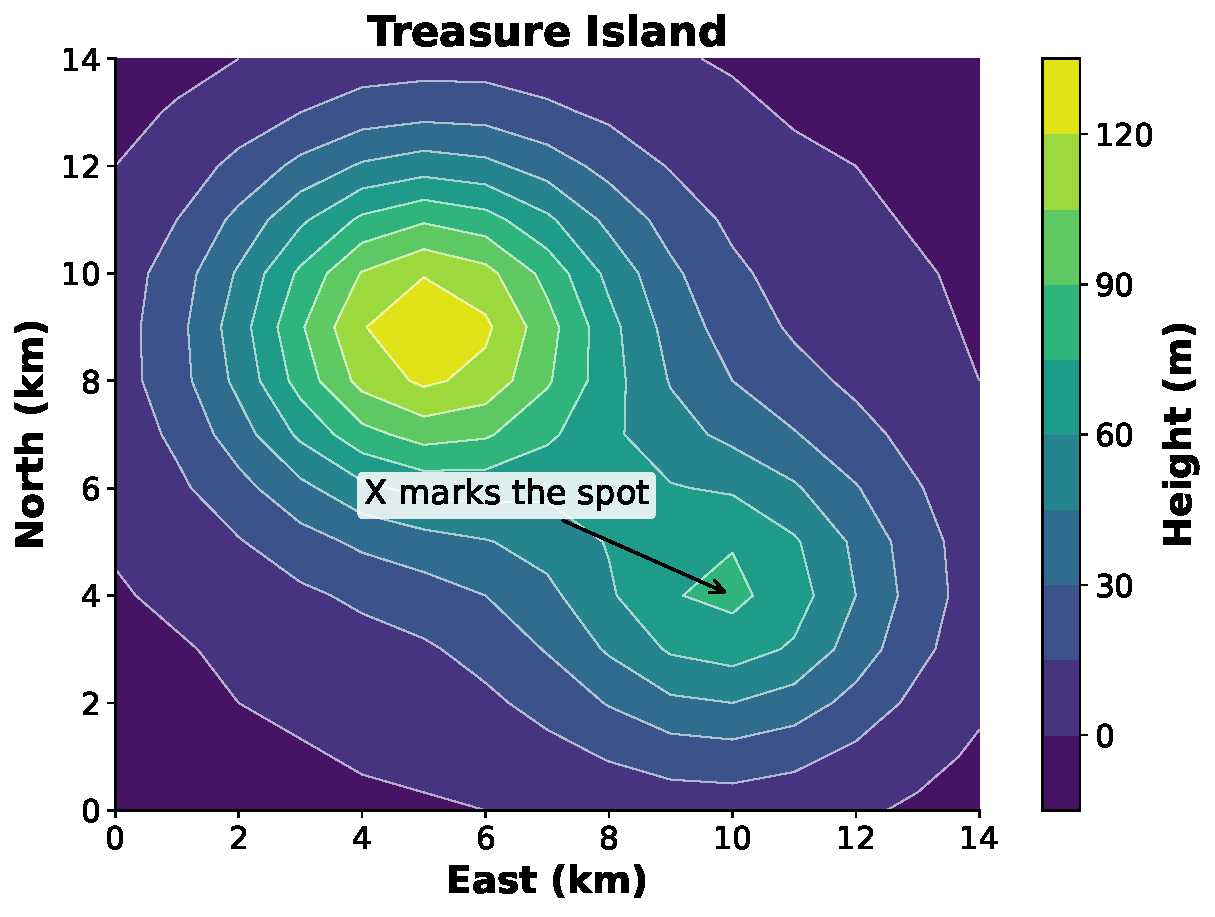
\includegraphics[width=0.72\textwidth,height=0.36\textheight,keepaspectratio]{figures/lesson08_example5_lesson8_my_program.pdf}
\captionof{figure}{Lesson 8, example 5: \code{lesson8\_\allowbreak{}my\_\allowbreak{}program.\allowbreak{}png}.}
\end{minipage}\end{center}
\begin{goodtoknow}
\begin{itemize}
  \item Those are all the charts! \code{sdata.\allowbreak{}words()} lists every word and \code{sdata.\allowbreak{}help(\textquotedbl{}word\textquotedbl{})} explains any of them. Lessons 9 to 12 teach tables: how to look at your data, clean it and sum it up before you draw it.
  \item Your own data: save it from Excel as \code{.\allowbreak{}xlsx} or \code{.\allowbreak{}csv}, then chart = \code{sdata.\allowbreak{}chart(\textquotedbl{}my\_\allowbreak{}file.\allowbreak{}xlsx\textquotedbl{})}. If a column name is spelt wrong, simplydata tells you the right one.
\end{itemize}
\end{goodtoknow}
\begin{tryit}
\begin{enumerate}
  \item Write your own program, from an empty file, for a question you care about.
  \item Use any example table, or your own. Give it a title, axis names and a note.
  \item Make a second chart of the same table, put the two charts side by side and save the page as a PDF.
\end{enumerate}
Worked solutions: page~\pageref{solutions:8}, or type \code{sdata.\allowbreak{}lesson(8,\allowbreak{} solutions=True)}.
\end{tryit}
\par\noindent{\small\sffamily\textbf{Words in this lesson:} \hyperref[word:second-y]{\code{chart.\allowbreak{}second\_\allowbreak{}y()}}, \hyperref[word:zoom-box]{\code{chart.\allowbreak{}zoom\_\allowbreak{}box()}}, \hyperref[word:heatmap]{\code{chart.\allowbreak{}heatmap()}}, \hyperref[word:label-colour-bar]{\code{chart.\allowbreak{}label\_\allowbreak{}colour\_\allowbreak{}bar()}}, \hyperref[word:size]{\code{chart.\allowbreak{}size()}}, \hyperref[word:animate]{\code{chart.\allowbreak{}animate()}}, \hyperref[word:contour]{\code{chart.\allowbreak{}contour()}}, \hyperref[word:note]{\code{chart.\allowbreak{}note()}}, \hyperref[word:style]{\code{chart.\allowbreak{}style()}}, \hyperref[word:sdata.words]{\code{sdata.\allowbreak{}words()}}, \hyperref[word:sdata.help]{\code{sdata.\allowbreak{}help()}}.\par}

\chapter{Tables: open one and look at it}\label{lesson:9}
\begin{learnbox}
\begin{itemize}
  \item how to turn data into a simplydata table
  \item how to look at the first and last rows, and the names of the columns
  \item how to describe every column and count what is in it
\end{itemize}
\end{learnbox}
\section*{Example 1}
Before you draw, look at your data. \code{sdata.\allowbreak{}table} gives you plain words for that.
\begin{lstlisting}[style=py]
import simplydata as sdata
table = sdata.table(sdata.example("marks"))
print(table)
table.show_first_rows(5)
table.show_last_rows(3)
print(table.column_names())
table.describe_columns()
table.count_rows()
\end{lstlisting}
\whateachline
\begin{lineexplain}
  \item[1] Load simplydata.
  \item[2] Make a table from the practice marks. For your own file, write \code{sdata.\allowbreak{}table(\textquotedbl{}my\_\allowbreak{}file.\allowbreak{}xlsx\textquotedbl{})}.
  \item[3] Print the table. The first line says how many rows and columns it has. Then come the first 10 rows.
  \item[4] Show only the first 5 rows.
  \item[5] Show the last 3 rows.
  \item[6] Print the names of the columns.
  \item[7] Describe every column: is it numbers or text, how many cells are empty, and the smallest, biggest and average number.
  \item[8] Count the rows, and say the answer in a sentence. One row is one child in one test.
\end{lineexplain}
\printedoutput{output/lesson09_example1.txt}
\section*{Example 2}
\code{count\_\allowbreak{}each} counts how often each different value comes up.
\begin{lstlisting}[style=py]
import simplydata as sdata
table = sdata.table(sdata.example("fruit"))
table.show_first_rows()
table.count_each("fruit")
table.count_each("shop")
\end{lstlisting}
\whateachline
\begin{lineexplain}
  \item[1] Load simplydata.
  \item[2] Make a table of fruit sold by two shops.
  \item[3] Show the first rows. With nothing in the brackets you get 5.
  \item[4] For each fruit: in how many rows it comes up. It says the answer in a sentence, and gives back a small table that also has the percent of all the rows.
  \item[5] The same for each shop.
\end{lineexplain}
\printedoutput{output/lesson09_example2.txt}
\section*{Example 3}
\code{sdata.\allowbreak{}table} can read many files at once. Here we first save two small files, then read them back together.
\begin{lstlisting}[style=py]
import simplydata as sdata
weather = sdata.table(sdata.example("weather"))
weather.keep_first_rows(12)
weather.save("lesson9_part1.csv")
weather.start_again()
weather.keep_last_rows(12)
weather.save("lesson9_part2.csv")
both = sdata.table("lesson9_part*.csv")
both.count_each("file")
both.show(rows=3)
\end{lstlisting}
\whateachline
\begin{lineexplain}
  \item[1] Load simplydata.
  \item[2] Make a table of the weather.
  \item[3] Keep the first 12 rows: one city, a whole year.
  \item[4] Save them as a CSV file.
  \item[5] Back to the whole table.
  \item[6] Keep the last 12 rows: another city.
  \item[7] Save them as a second file.
  \item[8] Read every file whose name fits the pattern (* stands for any text) and stack them. A new column, \code{\textquotedbl{}file\textquotedbl{}}, says where each row came from.
  \item[9] 12 rows from each file.
  \item[10] Show the first 3 rows with every column. \code{both.\allowbreak{}show()} shows the whole table.
\end{lineexplain}
\printedoutput{output/lesson09_example3.txt}
\begin{goodtoknow}
\begin{itemize}
  \item Looking never changes the table. Only steps that say what they change (\code{keep\_\allowbreak{}rows}, \code{sort\_\allowbreak{}by} ...) do, and lesson 10 shows them.
  \item In Jupyter, VS Code or Spyder, write table on the last line of a cell to see it as a nice table.
  \item \code{sdata.\allowbreak{}table} reads the same files as \code{sdata.\allowbreak{}chart}: \code{.\allowbreak{}xlsx}, \code{.\allowbreak{}csv}, \code{.\allowbreak{}tsv}, \code{.\allowbreak{}parquet} and \code{.\allowbreak{}json}. For one sheet of an Excel file: \code{sdata.\allowbreak{}table(\textquotedbl{}results.\allowbreak{}xlsx\textquotedbl{},\allowbreak{} sheet=\textquotedbl{}2026\textquotedbl{})}.
  \item The row numbers on the left start at 0, as everywhere in Python.
  \item A folder works too: \code{sdata.\allowbreak{}table(\textquotedbl{}data/\textquotedbl{})} reads every table file in it. A web address works like a file name: \code{sdata.\allowbreak{}table(\textquotedbl{}https://example.\allowbreak{}org/data.\allowbreak{}csv\textquotedbl{})}.
  \item Files written in another way: \code{separator=\textquotedbl{};\textquotedbl{}}, \code{decimal\_\allowbreak{}mark=\textquotedbl{},\allowbreak{}\textquotedbl{}} (3,5 is three and a half), \code{thousands\_\allowbreak{}mark=\textquotedbl{}.\allowbreak{}\textquotedbl{}}, \code{empty\_\allowbreak{}values=[\textquotedbl{}NA\textquotedbl{},\allowbreak{} \textquotedbl{}-\textquotedbl{}]}, \code{skip\_\allowbreak{}rows=2} and \code{encoding=\textquotedbl{}latin-1\textquotedbl{}}.
\end{itemize}
\end{goodtoknow}
\begin{tryit}
\begin{enumerate}
  \item Make a table of \code{sdata.\allowbreak{}example(\textquotedbl{}weather\textquotedbl{})}. How many rows does it have?
  \item Describe its columns. Which column has the biggest numbers?
  \item Count each \code{\textquotedbl{}city\textquotedbl{}}. Does every city have the same number of rows?
\end{enumerate}
Worked solutions: page~\pageref{solutions:9}, or type \code{sdata.\allowbreak{}lesson(9,\allowbreak{} solutions=True)}.
\end{tryit}
\par\noindent{\small\sffamily\textbf{Words in this lesson:} \hyperref[word:sdata.table]{\code{sdata.\allowbreak{}table()}}, \hyperref[word:table.show-first-rows]{\code{table.\allowbreak{}show\_\allowbreak{}first\_\allowbreak{}rows()}}, \hyperref[word:table.show-last-rows]{\code{table.\allowbreak{}show\_\allowbreak{}last\_\allowbreak{}rows()}}, \hyperref[word:table.column-names]{\code{table.\allowbreak{}column\_\allowbreak{}names()}}, \hyperref[word:table.describe-columns]{\code{table.\allowbreak{}describe\_\allowbreak{}columns()}}, \hyperref[word:table.count-rows]{\code{table.\allowbreak{}count\_\allowbreak{}rows()}}, \hyperref[word:table.count-each]{\code{table.\allowbreak{}count\_\allowbreak{}each()}}, \hyperref[word:table.show]{\code{table.\allowbreak{}show()}}.\par}

\chapter{Tables: choose rows and columns, and undo}\label{lesson:10}
\begin{learnbox}
\begin{itemize}
  \item how to keep only the columns and rows you want
  \item how to sort the rows
  \item how to take a step back, and start again
  \item how to save your table
\end{itemize}
\end{learnbox}
\section*{Example 1}
A table is changed in small steps, like a chart. Each step says what it did.
\begin{lstlisting}[style=py]
import simplydata as sdata
table = sdata.table(sdata.example("marks"))
table.keep_columns("name", "subject", "marks")
table.keep_rows("subject", equal_to="Maths")
table.keep_rows("marks", above=60)
table.sort_by("marks", biggest_first=True)
table.show_first_rows(10)
table.steps()
table.undo()
table.start_again()
print(table)
\end{lstlisting}
\whateachline
\begin{lineexplain}
  \item[1] Load simplydata.
  \item[2] Make a table of the marks.
  \item[3] Keep only these three columns, in this order.
  \item[4] Keep only the rows where the subject is Maths. simplydata says how many rows it kept.
  \item[5] Of those, keep only marks above 60.
  \item[6] Put the rows in order, the biggest mark first.
  \item[7] Show the first 10 rows: the best Maths marks.
  \item[8] List every step you did, in order.
  \item[9] Take back the last step (the sorting).
  \item[10] Go back to the whole table, as it was at the start.
  \item[11] All 54 rows and 6 columns are back.
\end{lineexplain}
\printedoutput{output/lesson10_example1.txt}
\section*{Example 2}
\code{keep\_\allowbreak{}rows} and \code{remove\_\allowbreak{}rows} know many conditions. Then save what you made.
\begin{lstlisting}[style=py]
import simplydata as sdata
table = sdata.table(sdata.example("weather"))
table.keep_rows("month_number", between=[6, 8])
table.remove_rows("city", equal_to="Frostby")
table.remove_columns("wind_direction", "wind_speed")
table.rename_column("temperature", to="temp")
print(table)
table.save("lesson10_summer.xlsx")
\end{lstlisting}
\whateachline
\begin{lineexplain}
  \item[1] Load simplydata.
  \item[2] Make a table of the weather.
  \item[3] Keep the summer months: 6, 7 and 8. \code{between=} keeps both ends.
  \item[4] Remove the rows of the city Frostby.
  \item[5] Remove two columns we do not need.
  \item[6] Give the column \code{\textquotedbl{}temperature\textquotedbl{}} the shorter name \code{\textquotedbl{}temp\textquotedbl{}}.
  \item[7] Look at what is left: 6 rows and 5 columns.
  \item[8] Save the table as an Excel file. A name ending in \code{.\allowbreak{}csv} saves a CSV file.
\end{lineexplain}
\printedoutput{output/lesson10_example2.txt}
\section*{Example 3}
A condition can also be written out, with and, or, not and brackets. And \code{keep\_\allowbreak{}biggest\_\allowbreak{}rows} keeps the top rows of each group.
\begin{lstlisting}[style=py]
import simplydata as sdata
table = sdata.table(sdata.example("marks"))
table.keep_rows("marks > 60 and subject == 'Maths'")
table.undo()
table.remove_rows("hours < 3 or class in ['B', 'C']")
table.start_again()
table.keep_biggest_rows(2, by="marks", for_each="subject")
table.show()
\end{lstlisting}
\whateachline
\begin{lineexplain}
  \item[1] Load simplydata.
  \item[2] Make a table of the marks.
  \item[3] Keep the rows where both are true: a mark above 60, in Maths. Text goes in quotes, and == means \code{\textquotedbl{}is equal to\textquotedbl{}}.
  \item[4] Back to all the rows.
  \item[5] Remove the rows where at least one is true: under 3 hours of study, or class B or C.
  \item[6] Back to the whole table.
  \item[7] Keep the 2 best marks in each subject: 6 rows.
  \item[8] Show the whole (small) table.
\end{lineexplain}
\printedoutput{output/lesson10_example3.txt}
\begin{goodtoknow}
\begin{itemize}
  \item Conditions for \code{keep\_\allowbreak{}rows} and \code{remove\_\allowbreak{}rows}: above, below, \code{at\_\allowbreak{}least}, \code{at\_\allowbreak{}most}, \code{equal\_\allowbreak{}to}, \code{not\_\allowbreak{}equal\_\allowbreak{}to}, between, \code{one\_\allowbreak{}of}, contains, \code{starts\_\allowbreak{}with}, \code{ends\_\allowbreak{}with} and \code{is\_\allowbreak{}empty}.
  \item \code{one\_\allowbreak{}of=} takes a list: \code{table.\allowbreak{}keep\_\allowbreak{}rows(\textquotedbl{}subject\textquotedbl{},\allowbreak{} one\_\allowbreak{}of=[\textquotedbl{}Maths\textquotedbl{},\allowbreak{} \textquotedbl{}Science\textquotedbl{}])}.
  \item \code{undo()} takes back one step at a time. \code{start\_\allowbreak{}again()} is a step too, so \code{undo()} can take it back.
  \item Your file is never changed: only \code{table.\allowbreak{}save(.\allowbreak{}.\allowbreak{}.\allowbreak{})} writes a file.
  \item Written conditions use == != \textless{} \textless{}= \textgreater{} \textgreater{}=, and, or, not, brackets, in [...] and is empty. An empty cell never meets a condition, and not does not change that: \code{\textquotedbl{}not (marks \textgreater{} 50)\textquotedbl{}} leaves out empty marks too. To find them, write \code{\textquotedbl{}marks is empty\textquotedbl{}}. A note says how many rows had an empty cell.
  \item Dates go in quotes as year-month-day: \code{table.\allowbreak{}keep\_\allowbreak{}rows(\textquotedbl{}date \textgreater{} '2026-03-01'\textquotedbl{})}, or \code{table.\allowbreak{}keep\_\allowbreak{}rows(\textquotedbl{}date\textquotedbl{},\allowbreak{} after=\textquotedbl{}2026-03-01\textquotedbl{})}.
\end{itemize}
\end{goodtoknow}
\begin{tryit}
\begin{enumerate}
  \item In the marks table, keep only class \code{\textquotedbl{}B\textquotedbl{}} and sort by \code{\textquotedbl{}hours\textquotedbl{}}. Who studied the longest?
  \item Undo the sorting, then sort by name instead.
  \item Keep 5 random rows with \code{table.\allowbreak{}keep\_\allowbreak{}random\_\allowbreak{}rows(5,\allowbreak{} seed=1)} and save them as \code{\textquotedbl{}five.\allowbreak{}csv\textquotedbl{}}.
  \item With one written condition, keep the rows with marks below 50 or hours above 8. How many rows are there?
\end{enumerate}
Worked solutions: page~\pageref{solutions:10}, or type \code{sdata.\allowbreak{}lesson(10,\allowbreak{} solutions=True)}.
\end{tryit}
\par\noindent{\small\sffamily\textbf{Words in this lesson:} \hyperref[word:table.keep-columns]{\code{table.\allowbreak{}keep\_\allowbreak{}columns()}}, \hyperref[word:table.keep-rows]{\code{table.\allowbreak{}keep\_\allowbreak{}rows()}}, \hyperref[word:table.sort-by]{\code{table.\allowbreak{}sort\_\allowbreak{}by()}}, \hyperref[word:table.steps]{\code{table.\allowbreak{}steps()}}, \hyperref[word:table.undo]{\code{table.\allowbreak{}undo()}}, \hyperref[word:table.start-again]{\code{table.\allowbreak{}start\_\allowbreak{}again()}}, \hyperref[word:table.remove-rows]{\code{table.\allowbreak{}remove\_\allowbreak{}rows()}}, \hyperref[word:table.remove-columns]{\code{table.\allowbreak{}remove\_\allowbreak{}columns()}}, \hyperref[word:table.rename-column]{\code{table.\allowbreak{}rename\_\allowbreak{}column()}}, \hyperref[word:table.save]{\code{table.\allowbreak{}save()}}, \hyperref[word:table.keep-random-rows]{\code{table.\allowbreak{}keep\_\allowbreak{}random\_\allowbreak{}rows()}}, \hyperref[word:table.keep-biggest-rows]{\code{table.\allowbreak{}keep\_\allowbreak{}biggest\_\allowbreak{}rows()}}.\par}

\chapter{Tables: clean the data and add new columns}\label{lesson:11}
\begin{learnbox}
\begin{itemize}
  \item how to find and fill empty cells
  \item how to fix columns: numbers written as text, extra spaces, wrong values
  \item how to add new columns, in plain words or like a sum in maths
  \item what long and wide tables are
\end{itemize}
\end{learnbox}
\section*{Example 1}
Real data often has empty cells. The practice tables have none, so we make some first.
\begin{lstlisting}[style=py]
import simplydata as sdata
table = sdata.table(sdata.example("marks"))
table.replace_values("marks", [61, 73], with_value=None)
table.count_empty_cells()
table.fill_empty_cells("marks", with_the="average")
table.undo()
table.remove_rows_with_empty_cells("marks")
print(table)
\end{lstlisting}
\whateachline
\begin{lineexplain}
  \item[1] Load simplydata.
  \item[2] Make a table of the marks.
  \item[3] Make every mark of 61 or 73 empty. \code{with\_\allowbreak{}value=None} means an empty cell.
  \item[4] Show how many empty cells each column has.
  \item[5] Fill the empty marks with the average of the other marks.
  \item[6] Changed your mind? Take it back: the cells are empty again.
  \item[7] This time remove the rows with an empty cell in marks.
  \item[8] Some rows fewer than at the start.
\end{lineexplain}
\printedoutput{output/lesson11_example1.txt}
\section*{Example 2}
Data typed by people is often untidy. These words fix whole columns at once.
\begin{lstlisting}[style=py]
import simplydata as sdata
table = sdata.table({"name": ["  Asha", "ben ", "Chen"], "height": ["144", "152", "unknown"]})
table.remove_extra_spaces("name")
table.replace_values("name", "ben", with_value="Ben")
table.make_numbers("height")
table.describe_columns()
\end{lstlisting}
\whateachline
\begin{lineexplain}
  \item[1] Load simplydata.
  \item[2] Make a small table by hand: each column name, then its values in a list.
  \item[3] Take away the spaces before and after the names.
  \item[4] Write \code{\textquotedbl{}ben\textquotedbl{}} with a capital letter.
  \item[5] Turn the heights from text into numbers. \code{\textquotedbl{}unknown\textquotedbl{}} is not a number, so that cell becomes empty, and simplydata tells you.
  \item[6] Now height is a column of numbers.
\end{lineexplain}
\printedoutput{output/lesson11_example2.txt}
\section*{Example 3}
A new column can be worked out from other columns, in plain words.
\begin{lstlisting}[style=py]
import simplydata as sdata
table = sdata.table(sdata.example("marks"))
table.add_column("marks_per_hour", by_dividing=["marks", "hours"])
table.add_group_column("grade", from_column="marks", cut_at=[40, 60, 80], names=["D", "C", "B", "A"])
table.show_first_rows()
table.count_each("grade")
\end{lstlisting}
\whateachline
\begin{lineexplain}
  \item[1] Load simplydata.
  \item[2] Make a table of the marks.
  \item[3] A new column called \code{\textquotedbl{}marks\_\allowbreak{}per\_\allowbreak{}hour\textquotedbl{}}: the marks divided by the hours.
  \item[4] A grade for each mark: below 40 is D, 40 to 59 is C, 60 to 79 is B, 80 and more is A.
  \item[5] Look at the two new columns on the right.
  \item[6] How many of each grade?
\end{lineexplain}
\printedoutput{output/lesson11_example3.txt}
\section*{Example 4}
Or write the new column like a sum in maths. Here each subject first gets its own column: the table goes from long to wide.
\begin{lstlisting}[style=py]
import simplydata as sdata
table = sdata.table(sdata.example("marks"))
table.keep_columns("name", "class", "subject", "marks")
table.turn_rows_into_columns(names_from="subject", values_from="marks")
table.add_column("total", "Maths + Science + English")
table.add_column("average", "total / 3")
table.add_rank_column("place", from_column="total")
table.sort_by("place")
table.show_first_rows()
\end{lstlisting}
\whateachline
\begin{lineexplain}
  \item[1] Load simplydata.
  \item[2] Make a table of the marks.
  \item[3] Keep the columns we need.
  \item[4] Make one column for each subject: Maths, Science and English. Each child now has one row.
  \item[5] A new column \code{\textquotedbl{}total\textquotedbl{}}: the three marks added up.
  \item[6] The average of the three marks.
  \item[7] Each child's place: 1 for the biggest total.
  \item[8] Put the rows in order of place.
  \item[9] Who came first?
\end{lineexplain}
\printedoutput{output/lesson11_example4.txt}
\section*{Example 5}
The shop table has real dates and some empty cells: days when the till broke. Look where they are, then fill them.
\begin{lstlisting}[style=py]
import simplydata as sdata
table = sdata.table(sdata.example("shop"))
table.count_empty_cells()
look = table.chart()
look.empty_cells()
look.save("lesson11_empty_cells.png")
table.add_is_empty_column("sales_was_empty", from_column="sales")
table.fill_empty_cells("sales", with_the="line between neighbours", sorted_by="date", for_each="shop")
table.add_date_part_column("weekday", from_column="date", part="weekday name")
table.add_rolling_column("sales_7_days", from_column="sales", window=7, for_each="shop", sorted_by="date")
table.show(rows=8)
\end{lstlisting}
\whateachline
\begin{lineexplain}
  \item[1] Load simplydata.
  \item[2] Daily sales of two shops, January to March 2026.
  \item[3] 10 empty sales and 5 empty customer counts.
  \item[4] A chart of the table, to see where the empty cells are.
  \item[5] One strip per column and one line per row: empty cells are coloured, and each column says how many it has.
  \item[6] Save it.
  \item[7] Before filling: a True/False column that remembers which sales were empty.
  \item[8] Fill each gap on the straight line between the day before and the day after, in date order, for each shop on its own. A gap at the very start or end has a neighbour on one side only, so it stays empty, and a note says so.
  \item[9] A new column with the weekday of each date.
  \item[10] The average of each day and the 6 days before it: a 7-day moving average, which smooths out the busy weekends.
  \item[11] Look at the first 8 rows.
\end{lineexplain}
\printedoutput{output/lesson11_example5.txt}
\begin{center}\begin{minipage}{\linewidth}\centering
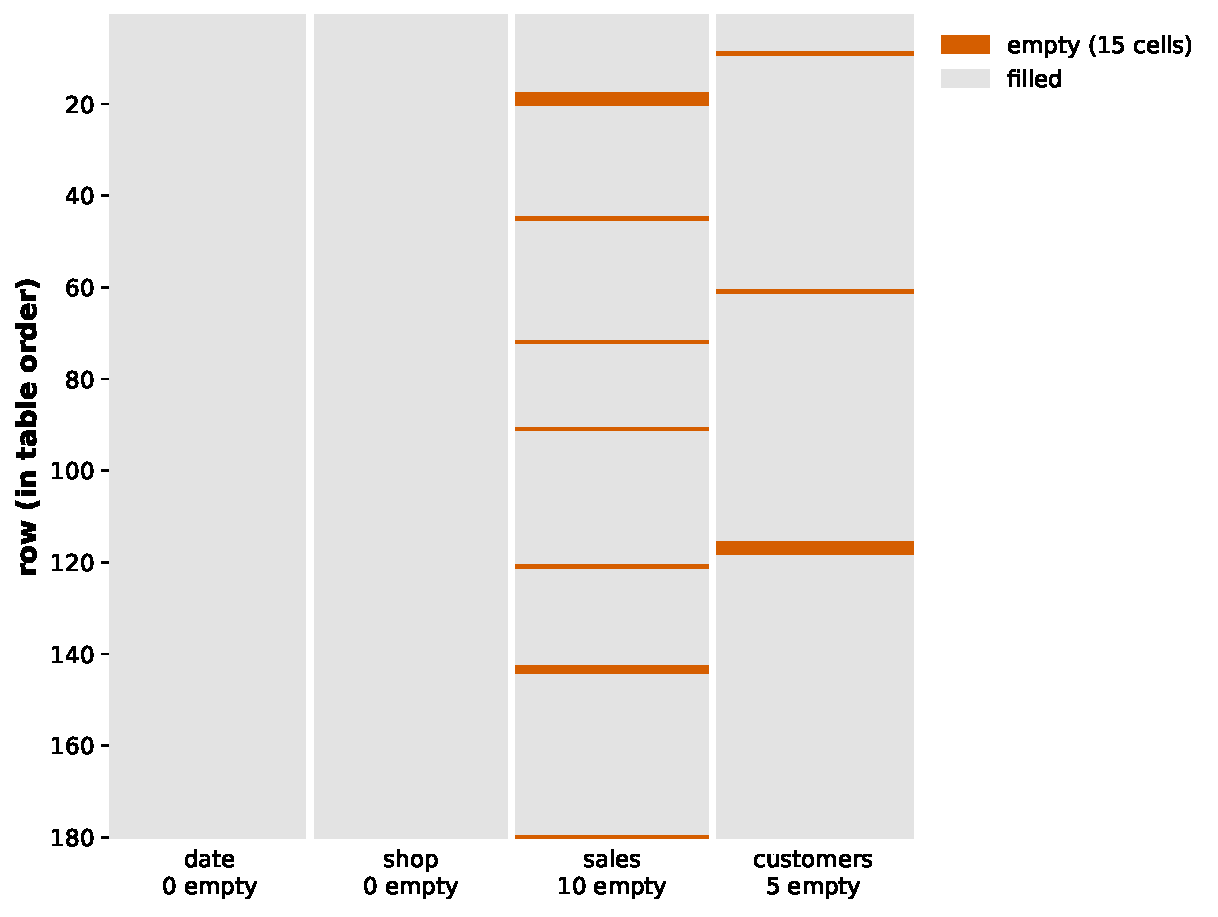
\includegraphics[width=0.72\textwidth,height=0.36\textheight,keepaspectratio]{figures/lesson11_example5_lesson11_empty_cells.pdf}
\captionof{figure}{Lesson 11, example 5: \code{lesson11\_\allowbreak{}empty\_\allowbreak{}cells.\allowbreak{}png}.}
\end{minipage}\end{center}
\section*{Example 6}
Names and dates typed in by people often need taking apart.
\begin{lstlisting}[style=py]
import simplydata as sdata
table = sdata.table({"name": ["Asha Rao", "Ben Lee", "Chen Wu"], "born": ["04/30/2014", "12/25/2013", "07/03/2014"], "height": [144.37, 152.81, 139.5]})
table.split_column("name", separator=" ", into=["first_name", "family_name"])
table.add_text_part_column("initial", from_column="first_name", first_characters=1)
table.replace_text("family_name", "Lee", with_value="Li")
table.make_dates("born", order="month day year")
table.add_date_part_column("month_born", from_column="born", part="month name")
table.change_column("height", "height / 100")
table.round_to("height", 2)
table.show()
\end{lstlisting}
\whateachline
\begin{lineexplain}
  \item[1] Load simplydata.
  \item[2] A small table typed by hand. The birthdays are written month first, as in the USA.
  \item[3] Split each name at the space into two new columns.
  \item[4] The first letter of each first name.
  \item[5] Replace a piece of text inside the cells.
  \item[6] Turn the birthdays into dates. \code{order=} says how they are written, so 07/03/2014 is read as 3 July and not as 7 March.
  \item[7] The month of each birthday, as a word.
  \item[8] Change the heights from centimetres to metres, in the same column.
  \item[9] Round them to 2 decimal places.
  \item[10] Look at the whole table.
\end{lineexplain}
\printedoutput{output/lesson11_example6.txt}
\begin{goodtoknow}
\begin{itemize}
  \item Formulas know more maths than + - * /: sqrt, log, exp, sin, cos, tan, pi, and special functions such as erf, gamma, lgamma, beta and besselJ: \code{table.\allowbreak{}add\_\allowbreak{}column(\textquotedbl{}z\textquotedbl{},\allowbreak{} formula=\textquotedbl{}erf(marks / 100)\textquotedbl{})}.
  \item Long or wide? A long table has one row for each measurement: the marks table has a row for each child in each subject. A wide table puts the measurements of one child side by side, one column per subject. Charts and tests like long tables (also called tidy data); sums across columns, like the total above, need wide ones.
  \item Filling empty cells is called imputation. Filling with the average makes the values look less spread out than they really are, so say in your report how you filled them. \code{with\_\allowbreak{}the=\textquotedbl{}median\textquotedbl{}}, \code{\textquotedbl{}value above\textquotedbl{}} or \code{\textquotedbl{}value below\textquotedbl{}} and \code{with\_\allowbreak{}value=0} work too.
  \item \code{remove\_\allowbreak{}rows\_\allowbreak{}with\_\allowbreak{}empty\_\allowbreak{}cells()} with nothing in the brackets removes every row that has an empty cell in any column.
  \item More fixing words: \code{make\_\allowbreak{}text}, \code{make\_\allowbreak{}dates}, \code{make\_\allowbreak{}lowercase} and \code{make\_\allowbreak{}uppercase}.
  \item Plain words for new columns: \code{by\_\allowbreak{}adding=}, \code{by\_\allowbreak{}subtracting=}, \code{by\_\allowbreak{}multiplying=} and \code{by\_\allowbreak{}dividing=}, or \code{from\_\allowbreak{}column=} with \code{plus=}, \code{minus=}, \code{times=} or \code{divide\_\allowbreak{}by=}.
  \item In a maths-style column, a column name with spaces goes in backticks: \code{\textquotedbl{}`max temp` - 2\textquotedbl{}}.
  \item \code{with\_\allowbreak{}the=\textquotedbl{}line between neighbours\textquotedbl{}} is linear interpolation. It suits values that change smoothly, like sales from day to day; it cannot know about a sudden jump. Keep a True/False column of what you filled, and say in your report how you filled it.
  \item Charts say it too: when a chart leaves out rows because of empty cells, one line tells you how many.
  \item Row after row: \code{add\_\allowbreak{}previous\_\allowbreak{}value\_\allowbreak{}column} gives the value of the row before, and \code{add\_\allowbreak{}change\_\allowbreak{}column} the change since then (\code{in\_\allowbreak{}percent=True} for a percent).
\end{itemize}
\end{goodtoknow}
\begin{tryit}
\begin{enumerate}
  \item In the first example, fill the empty marks with the median instead of the average.
  \item Add a column \code{\textquotedbl{}height\_\allowbreak{}m\textquotedbl{}} with the height in metres: \code{from\_\allowbreak{}column=\textquotedbl{}height\textquotedbl{}}, \code{divide\_\allowbreak{}by=100}.
  \item In the last example, add a column \code{\textquotedbl{}best\_\allowbreak{}two\textquotedbl{}} with the formula \code{\textquotedbl{}total - English\textquotedbl{}}.
  \item In the shop example, add a column \code{\textquotedbl{}change\textquotedbl{}} with the change in sales from the day before, \code{for\_\allowbreak{}each=\textquotedbl{}shop\textquotedbl{}} and \code{sorted\_\allowbreak{}by=\textquotedbl{}date\textquotedbl{}} (\code{add\_\allowbreak{}change\_\allowbreak{}column}).
\end{enumerate}
Worked solutions: page~\pageref{solutions:11}, or type \code{sdata.\allowbreak{}lesson(11,\allowbreak{} solutions=True)}.
\end{tryit}
\par\noindent{\small\sffamily\textbf{Words in this lesson:} \hyperref[word:table.replace-values]{\code{table.\allowbreak{}replace\_\allowbreak{}values()}}, \hyperref[word:table.count-empty-cells]{\code{table.\allowbreak{}count\_\allowbreak{}empty\_\allowbreak{}cells()}}, \hyperref[word:table.fill-empty-cells]{\code{table.\allowbreak{}fill\_\allowbreak{}empty\_\allowbreak{}cells()}}, \hyperref[word:table.remove-rows-with-empty-cells]{\code{table.\allowbreak{}remove\_\allowbreak{}rows\_\allowbreak{}with\_\allowbreak{}empty\_\allowbreak{}cells()}}, \hyperref[word:table.remove-extra-spaces]{\code{table.\allowbreak{}remove\_\allowbreak{}extra\_\allowbreak{}spaces()}}, \hyperref[word:table.make-numbers]{\code{table.\allowbreak{}make\_\allowbreak{}numbers()}}, \hyperref[word:table.add-column]{\code{table.\allowbreak{}add\_\allowbreak{}column()}}, \hyperref[word:table.add-group-column]{\code{table.\allowbreak{}add\_\allowbreak{}group\_\allowbreak{}column()}}, \hyperref[word:table.add-rank-column]{\code{table.\allowbreak{}add\_\allowbreak{}rank\_\allowbreak{}column()}}, \hyperref[word:table.turn-rows-into-columns]{\code{table.\allowbreak{}turn\_\allowbreak{}rows\_\allowbreak{}into\_\allowbreak{}columns()}}, \hyperref[word:table.add-is-empty-column]{\code{table.\allowbreak{}add\_\allowbreak{}is\_\allowbreak{}empty\_\allowbreak{}column()}}, \hyperref[word:empty-cells]{\code{chart.\allowbreak{}empty\_\allowbreak{}cells()}}, \hyperref[word:table.add-date-part-column]{\code{table.\allowbreak{}add\_\allowbreak{}date\_\allowbreak{}part\_\allowbreak{}column()}}, \hyperref[word:table.add-rolling-column]{\code{table.\allowbreak{}add\_\allowbreak{}rolling\_\allowbreak{}column()}}, \hyperref[word:table.split-column]{\code{table.\allowbreak{}split\_\allowbreak{}column()}}, \hyperref[word:table.add-text-part-column]{\code{table.\allowbreak{}add\_\allowbreak{}text\_\allowbreak{}part\_\allowbreak{}column()}}, \hyperref[word:table.replace-text]{\code{table.\allowbreak{}replace\_\allowbreak{}text()}}, \hyperref[word:table.make-dates]{\code{table.\allowbreak{}make\_\allowbreak{}dates()}}, \hyperref[word:table.change-column]{\code{table.\allowbreak{}change\_\allowbreak{}column()}}, \hyperref[word:table.round-to]{\code{table.\allowbreak{}round\_\allowbreak{}to()}}, \hyperref[word:table.add-change-column]{\code{table.\allowbreak{}add\_\allowbreak{}change\_\allowbreak{}column()}}.\par}

\chapter{Tables: summaries, and from a table to a chart}\label{lesson:12}
\begin{learnbox}
\begin{itemize}
  \item how to work out averages, totals and counts, for each group
  \item how to tell if two columns go together, and why that is not the same as a cause
  \item how to draw a table, and which rows a chart uses
  \item how to join two tables and turn columns into rows
\end{itemize}
\end{learnbox}
\section*{Example 1}
A summary turns many rows into a few numbers. It never changes your table, and it says its answer in a sentence.
\begin{lstlisting}[style=py]
import simplydata as sdata
table = sdata.table(sdata.example("marks"))
table.average_of("marks")
table.average_of("marks", for_each="class")
table.biggest_of("marks", for_each="subject")
table.correlation_between("hours", "marks")
\end{lstlisting}
\whateachline
\begin{lineexplain}
  \item[1] Load simplydata.
  \item[2] Make a table of the marks.
  \item[3] The average of all the marks: just one number.
  \item[4] One average for each class. \code{for\_\allowbreak{}each=} also gives back a new, small table.
  \item[5] The best mark in each subject.
  \item[6] Do more hours go with more marks? The answer is a number r from -1 to 1 (Pearson's correlation), explained in words.
\end{lineexplain}
\printedoutput{output/lesson12_example1.txt}
\section*{Example 2}
A summary for each group is a table too, so you can sort it and draw it.
\begin{lstlisting}[style=py]
import simplydata as sdata
table = sdata.table(sdata.example("fruit"))
totals = table.total_of("count", for_each="fruit")
totals.sort_by("total of count", biggest_first=True)
chart = totals.chart()
chart.bars(x="fruit", y="total of count")
chart.numbers_on_bars()
chart.save("lesson12_fruit.png")
\end{lstlisting}
\whateachline
\begin{lineexplain}
  \item[1] Load simplydata.
  \item[2] Make a table of fruit sales.
  \item[3] A new table called totals: one row per fruit, with a column \code{\textquotedbl{}total of count\textquotedbl{}}. table itself does not change.
  \item[4] Best seller first.
  \item[5] Start a chart from the summary table.
  \item[6] One bar per fruit.
  \item[7] Write the total on each bar.
  \item[8] Save the chart.
\end{lineexplain}
\printedoutput{output/lesson12_example2.txt}
\begin{center}\begin{minipage}{\linewidth}\centering
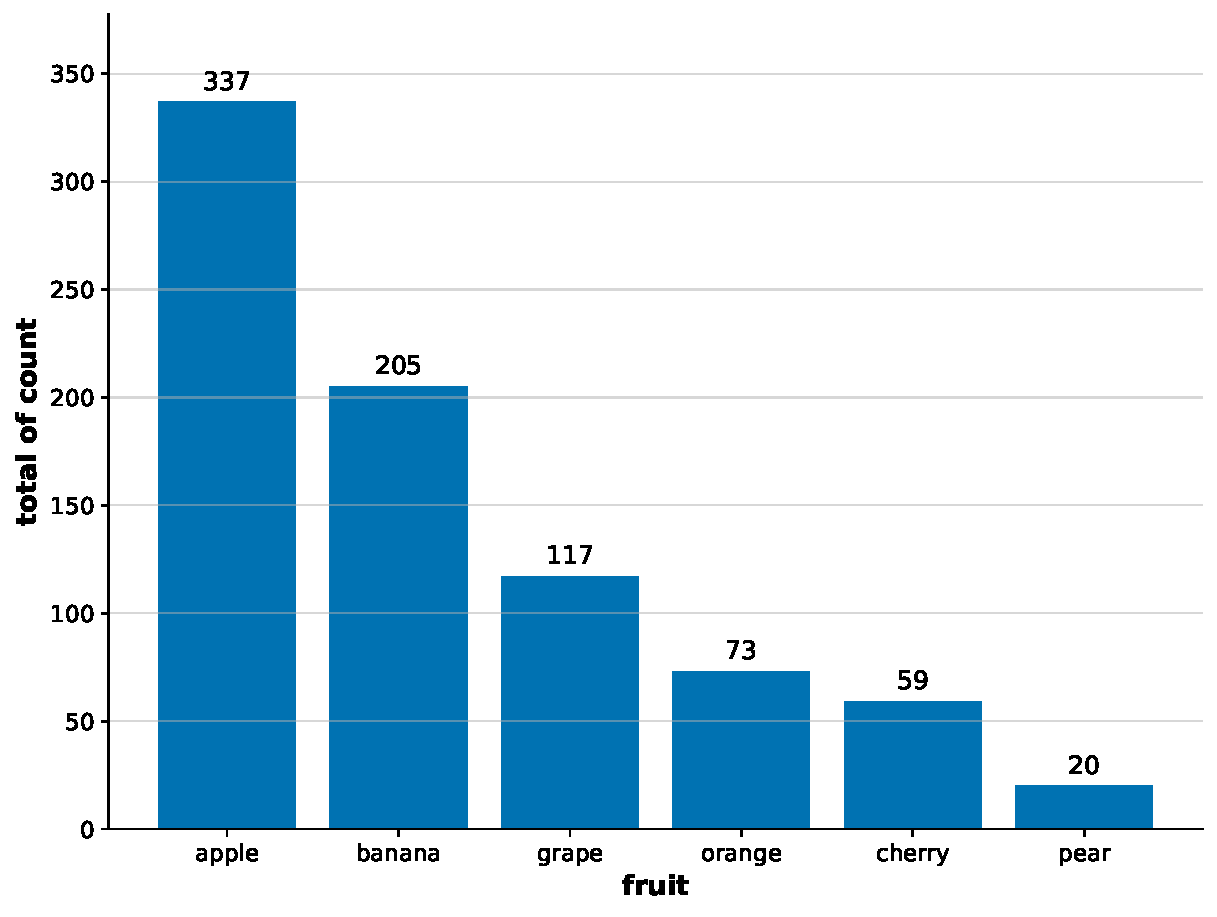
\includegraphics[width=0.72\textwidth,height=0.36\textheight,keepaspectratio]{figures/lesson12_example2_lesson12_fruit.pdf}
\captionof{figure}{Lesson 12, example 2: \code{lesson12\_\allowbreak{}fruit.\allowbreak{}png}.}
\end{minipage}\end{center}
\section*{Example 3}
A chart uses the table as it was when you made the chart. Table steps after it are for the next chart.
\begin{lstlisting}[style=py]
import simplydata as sdata
table = sdata.table(sdata.example("marks"))
table.keep_rows("class", equal_to="A")
all_tests = table.chart()
all_tests.dots(x="hours", y="marks")
table.keep_rows("subject", equal_to="Maths")
maths = table.chart()
maths.dots(x="hours", y="marks")
page = sdata.side_by_side(all_tests, maths, same_y=True)
page.save("lesson12_maths.png")
\end{lstlisting}
\whateachline
\begin{lineexplain}
  \item[1] Load simplydata.
  \item[2] Make a table of the marks.
  \item[3] Keep class A.
  \item[4] A chart of the table as it is now: every test of class A. \code{sdata.\allowbreak{}chart(table)} does the same.
  \item[5] Draw hours against marks.
  \item[6] A table step after the chart. The chart \code{all\_\allowbreak{}tests} does not change.
  \item[7] A second chart, of the table as it is now: only the Maths tests of class A.
  \item[8] Draw the same thing again.
  \item[9] Both charts on one page, with the same y-axis, so you can compare them.
  \item[10] Save the page.
\end{lineexplain}
\printedoutput{output/lesson12_example3.txt}
\begin{center}\begin{minipage}{\linewidth}\centering
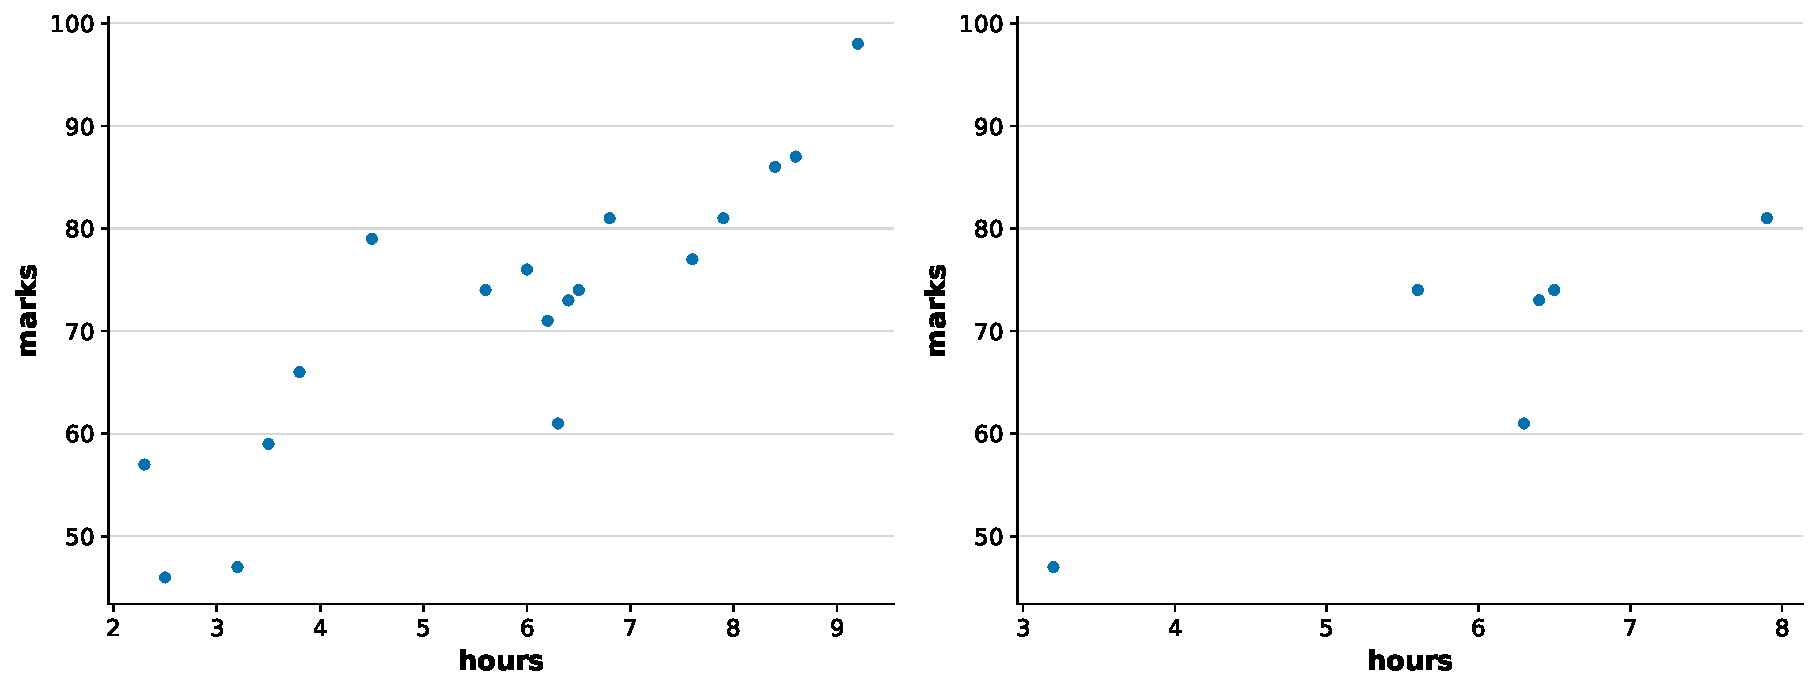
\includegraphics[width=0.72\textwidth,height=0.36\textheight,keepaspectratio]{figures/lesson12_example3_lesson12_maths.pdf}
\captionof{figure}{Lesson 12, example 3: \code{lesson12\_\allowbreak{}maths.\allowbreak{}png}.}
\end{minipage}\end{center}
\section*{Example 4}
Two tables can be joined: their rows are matched on a column they share.
\begin{lstlisting}[style=py]
import simplydata as sdata
table = sdata.table(sdata.example("marks"))
ages = {"name": ["Asha", "Ben", "Chen"], "age": [12, 13, 12]}
table.join_with(ages, using="name")
table.show_first_rows()
table.average_of("marks", for_each="age")
\end{lstlisting}
\whateachline
\begin{lineexplain}
  \item[1] Load simplydata.
  \item[2] Make a table of the marks.
  \item[3] A small table of ages, typed by hand: each column name, then its values.
  \item[4] Bring in the age, matching the rows on the name. Only children found in both tables stay.
  \item[5] Look: there is a new column, age.
  \item[6] The average mark at each age.
\end{lineexplain}
\printedoutput{output/lesson12_example4.txt}
\section*{Example 5}
Turning columns into rows makes a wide table long: the shape most charts like.
\begin{lstlisting}[style=py]
import simplydata as sdata
table = sdata.table({"name": ["Asha", "Ben", "Chen"], "test_1": [61, 73, 81], "test_2": [70, 68, 90]})
table.turn_columns_into_rows(["test_1", "test_2"], names_to="test", values_to="mark")
table.show_first_rows(6)
chart = table.chart()
chart.bars(x="name", y="mark", colour="test")
chart.save("lesson12_tests.png")
\end{lstlisting}
\whateachline
\begin{lineexplain}
  \item[1] Load simplydata.
  \item[2] A small, wide table: two tests, one column for each.
  \item[3] Put the two tests under each other. The new column \code{\textquotedbl{}test\textquotedbl{}} says which test, and \code{\textquotedbl{}mark\textquotedbl{}} holds the mark. Each child now has two rows.
  \item[4] Look at the new, long shape.
  \item[5] Start a chart from it.
  \item[6] Both tests side by side for each child.
  \item[7] Save it.
\end{lineexplain}
\printedoutput{output/lesson12_example5.txt}
\begin{center}\begin{minipage}{\linewidth}\centering
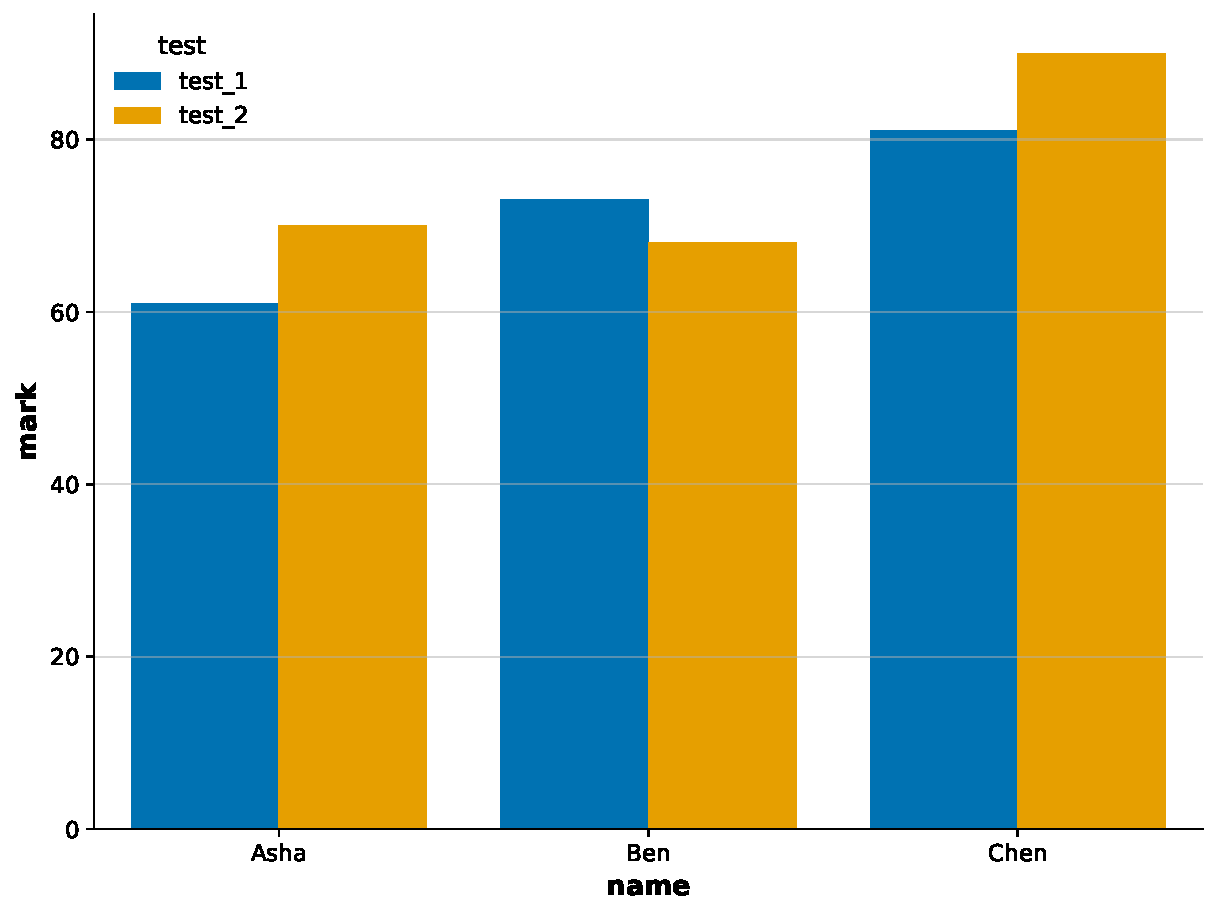
\includegraphics[width=0.72\textwidth,height=0.36\textheight,keepaspectratio]{figures/lesson12_example5_lesson12_tests.pdf}
\captionof{figure}{Lesson 12, example 5: \code{lesson12\_\allowbreak{}tests.\allowbreak{}png}.}
\end{minipage}\end{center}
\section*{Example 6}
\code{summary\_\allowbreak{}of} gives several measures at once, and \code{every=} sums up dates by week, month or year.
\begin{lstlisting}[style=py]
import simplydata as sdata
table = sdata.table(sdata.example("shop"))
table.summary_of("sales", for_each="shop", show=["average", "median", "standard deviation", "count", "empty cells"])
table.total_of("sales", for_each="date", every="month")
table.percent_of("sales", above=500, for_each="shop")
\end{lstlisting}
\whateachline
\begin{lineexplain}
  \item[1] Load simplydata.
  \item[2] Daily sales of two shops.
  \item[3] Five measures of each shop's sales in one tidy table. count counts the days with a number; empty cells counts the others.
  \item[4] The total sales of each month: \code{every=} puts the days of one month together.
  \item[5] On what percent of the days did each shop take more than 500? Each percent comes with its 95 \% confidence interval.
\end{lineexplain}
\printedoutput{output/lesson12_example6.txt}
\section*{Example 7}
A cross table puts one group down the side and another across the top. A correlation table compares many columns at once.
\begin{lstlisting}[style=py]
import simplydata as sdata
fruit = sdata.table(sdata.example("fruit"))
fruit.count_rows(for_each="shop", across="fruit")
fruit.count_different_values("fruit", for_each="shop")
marks = sdata.table(sdata.example("marks"))
marks.average_of("marks", for_each="class", across="subject")
marks.correlation_between("hours", "marks", "height")
\end{lstlisting}
\whateachline
\begin{lineexplain}
  \item[1] Load simplydata.
  \item[2] A table of fruit sales.
  \item[3] How many sales of each fruit in each shop: one row per shop, one column per fruit.
  \item[4] How many different fruits each shop sold.
  \item[5] A table of the marks.
  \item[6] The average mark of each class in each subject.
  \item[7] Every pair of the three columns at once: a correlation table, with the strongest pairs in words.
\end{lineexplain}
\printedoutput{output/lesson12_example7.txt}
\section*{Example 8}
More ways to sum up: percentiles, the most common value, and measures of shape.
\begin{lstlisting}[style=py]
import simplydata as sdata
marks = sdata.table(sdata.example("marks"))
marks.percentile_of("marks", 90, for_each="class")
marks.summary_of("marks", show=["median", "skewness", "coefficient of variation"], for_each="class")
school = sdata.table(sdata.example("school"))
school.most_common_of("days_absent")
\end{lstlisting}
\whateachline
\begin{lineexplain}
  \item[1] Load simplydata.
  \item[2] A table of the marks.
  \item[3] The 90th percentile: 90 \% of the marks are below it (86.3 in class A).
  \item[4] Skewness says if the values lean to one side (below 0: a longer tail of low marks); the coefficient of variation is the standard deviation divided by the average.
  \item[5] A table of pupils.
  \item[6] The most common number of days absent (the mode): 2.
\end{lineexplain}
\printedoutput{output/lesson12_example8.txt}
\begin{goodtoknow}
\begin{itemize}
  \item Correlation is not cause. Children who study more might also sleep more, or like the subject more; r only says that two columns go up and down together, not which one makes the other change.
  \item More summaries: \code{median\_\allowbreak{}of}, \code{total\_\allowbreak{}of}, \code{smallest\_\allowbreak{}of}, \code{biggest\_\allowbreak{}of}, \code{standard\_\allowbreak{}deviation\_\allowbreak{}of} and \code{count\_\allowbreak{}rows}. Each one can take \code{for\_\allowbreak{}each=}.
  \item A chart never changes its table, and a table step never changes a chart you already made. So one cleaned table can feed many charts.
  \item \code{table.\allowbreak{}add\_\allowbreak{}rows\_\allowbreak{}from(other)} puts the rows of another table under this one. \code{turn\_\allowbreak{}rows\_\allowbreak{}into\_\allowbreak{}columns} does the opposite of \code{turn\_\allowbreak{}columns\_\allowbreak{}into\_\allowbreak{}rows}.
  \item Lesson 13 teaches numbers, and lesson 14 the statistical tests: is a difference real, or could it be chance?
  \item Every summary skips empty cells and says how many it skipped. \code{summary\_\allowbreak{}of} can also show \code{\textquotedbl{}variance\textquotedbl{}}, \code{\textquotedbl{}standard error\textquotedbl{}}, \code{\textquotedbl{}confidence interval\textquotedbl{}}, \code{\textquotedbl{}range\textquotedbl{}} and \code{\textquotedbl{}interquartile range\textquotedbl{}}.
\end{itemize}
\end{goodtoknow}
\begin{tryit}
\begin{enumerate}
  \item Make the fruit totals \code{for\_\allowbreak{}each=\textquotedbl{}shop\textquotedbl{}} instead. Which shop sold more?
  \item Work out the average temperature \code{for\_\allowbreak{}each=\textquotedbl{}city\textquotedbl{}} in the weather table and draw it as bars.
  \item Is there a link between height and marks? Use \code{correlation\_\allowbreak{}between} to find out.
  \item Make a cross table of the average mark \code{for\_\allowbreak{}each=\textquotedbl{}subject\textquotedbl{}} \code{across=\textquotedbl{}class\textquotedbl{}}. Which class is best in Science?
\end{enumerate}
Worked solutions: page~\pageref{solutions:12}, or type \code{sdata.\allowbreak{}lesson(12,\allowbreak{} solutions=True)}.
\end{tryit}
\par\noindent{\small\sffamily\textbf{Words in this lesson:} \hyperref[word:table.average-of]{\code{table.\allowbreak{}average\_\allowbreak{}of()}}, \hyperref[word:table.biggest-of]{\code{table.\allowbreak{}biggest\_\allowbreak{}of()}}, \hyperref[word:table.correlation-between]{\code{table.\allowbreak{}correlation\_\allowbreak{}between()}}, \hyperref[word:table.total-of]{\code{table.\allowbreak{}total\_\allowbreak{}of()}}, \hyperref[word:table.chart]{\code{table.\allowbreak{}chart()}}, \hyperref[word:sdata.side-by-side]{\code{sdata.\allowbreak{}side\_\allowbreak{}by\_\allowbreak{}side()}}, \hyperref[word:table.join-with]{\code{table.\allowbreak{}join\_\allowbreak{}with()}}, \hyperref[word:table.turn-columns-into-rows]{\code{table.\allowbreak{}turn\_\allowbreak{}columns\_\allowbreak{}into\_\allowbreak{}rows()}}, \hyperref[word:table.add-rows-from]{\code{table.\allowbreak{}add\_\allowbreak{}rows\_\allowbreak{}from()}}, \hyperref[word:table.summary-of]{\code{table.\allowbreak{}summary\_\allowbreak{}of()}}, \hyperref[word:table.percent-of]{\code{table.\allowbreak{}percent\_\allowbreak{}of()}}, \hyperref[word:table.count-rows]{\code{table.\allowbreak{}count\_\allowbreak{}rows()}}, \hyperref[word:table.count-different-values]{\code{table.\allowbreak{}count\_\allowbreak{}different\_\allowbreak{}values()}}, \hyperref[word:table.percentile-of]{\code{table.\allowbreak{}percentile\_\allowbreak{}of()}}, \hyperref[word:table.most-common-of]{\code{table.\allowbreak{}most\_\allowbreak{}common\_\allowbreak{}of()}}.\par}

\chapter{Numbers: lists and grids of numbers}\label{lesson:13}
\begin{learnbox}
\begin{itemize}
  \item how to make a list of numbers, and a grid of them
  \item two ways to do maths: symbols make new numbers, words change the numbers you have
  \item how to keep some numbers, sum them up, and draw them
\end{itemize}
\end{learnbox}
\section*{Example 1}
Numbers are for when you have just numbers, not a table with named columns.
\begin{lstlisting}[style=py]
import simplydata as sdata
nums = sdata.numbers([12, 15, 9, 20, 14])
print(nums)
bigger = nums * 2
print(bigger)
nums.add(1)
nums.undo()
nums.keep_numbers(above=10)
nums.average()
nums.standard_deviation()
nums.steps()
\end{lstlisting}
\whateachline
\begin{lineexplain}
  \item[1] Load simplydata.
  \item[2] Make a list of five numbers and call it nums.
  \item[3] Look at them. The first line says how many there are.
  \item[4] Maths with symbols makes NEW numbers: every number times 2. nums itself does not change.
  \item[5] 24, 30, 18, 40 and 28.
  \item[6] Maths with words CHANGES the numbers you have: add 1 to each one.
  \item[7] Like a table, numbers can take back every word.
  \item[8] Keep only the numbers above 10. The same conditions as \code{keep\_\allowbreak{}rows}: above, below, between ...
  \item[9] The average of what is left, said in a sentence.
  \item[10] How spread out they are (divide by n - 1, as in pandas and R).
  \item[11] List the steps you did.
\end{lineexplain}
\printedoutput{output/lesson13_example1.txt}
\section*{Example 2}
Counting, random numbers and a chart.
\begin{lstlisting}[style=py]
import simplydata as sdata
months = sdata.numbers(1, to=12)
temps = sdata.numbers([4, 6, 9, 13, 17, 20, 22, 21, 17, 12, 8, 5])
chart = sdata.chart()
chart.lines(x=months, y=temps, dots=True)
chart.save("lesson13_line.png")
heights = sdata.random_numbers(how_many=200, average=150, standard_deviation=8, seed=1)
heights.median()
heights.percentile(90)
chart = heights.chart()
chart.histogram(x="value", bins=12)
chart.save("lesson13_heights.png")
\end{lstlisting}
\whateachline
\begin{lineexplain}
  \item[1] Load simplydata.
  \item[2] Count from 1 to 12. The end is included.
  \item[3] A temperature for each month.
  \item[4] Start an empty chart: the numbers go straight into the chart type.
  \item[5] Draw the temperatures as a line, month by month.
  \item[6] Save it.
  \item[7] 200 made-up heights that bunch around 150 in a bell shape (a normal distribution). \code{seed=1} gives the same numbers every time, so others can repeat your work.
  \item[8] The middle height.
  \item[9] The height that 90 \% of them are below.
  \item[10] Start a chart from the numbers. Their column is called value.
  \item[11] Count how many heights fall in each range.
  \item[12] Save it. Can you see the bell shape?
\end{lineexplain}
\printedoutput{output/lesson13_example2.txt}
\begin{center}\begin{minipage}{\linewidth}\centering
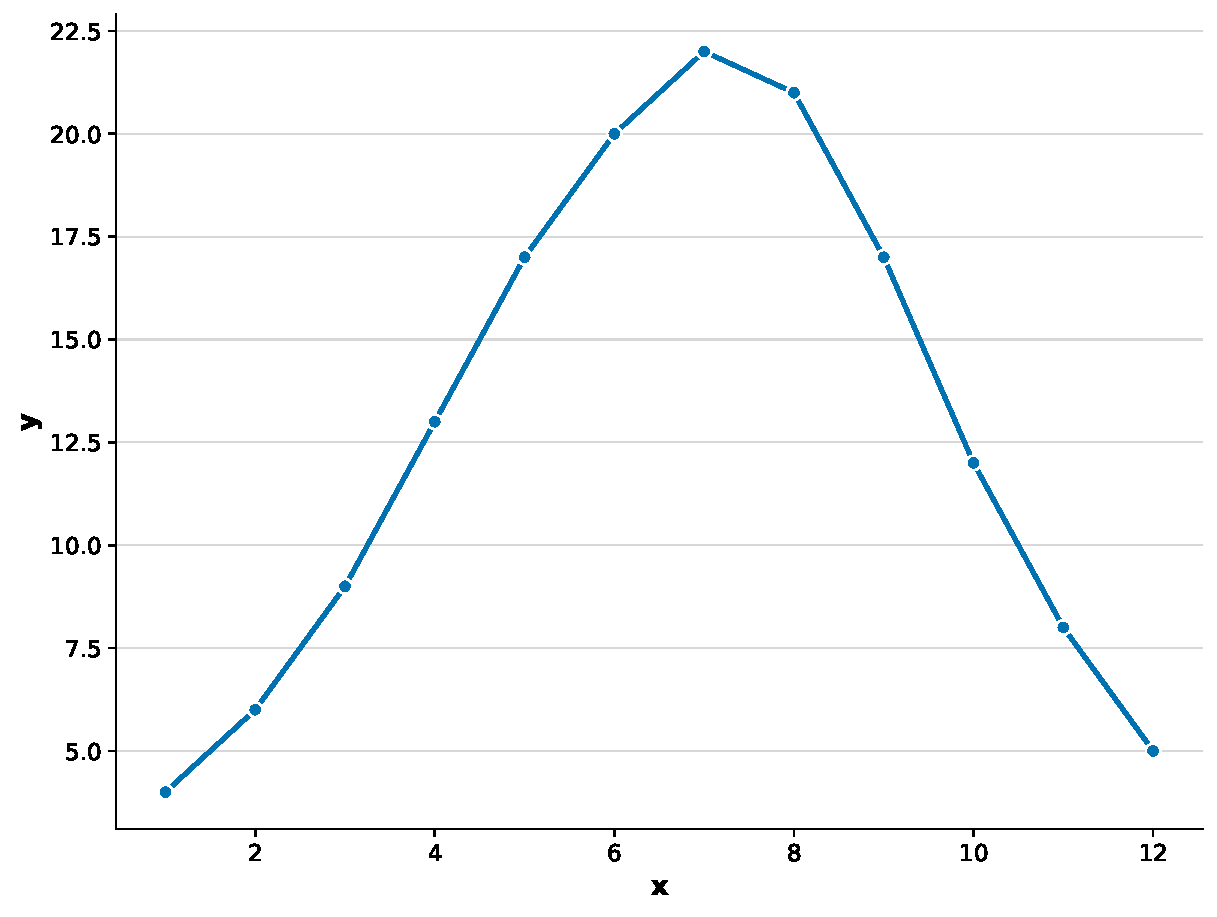
\includegraphics[width=0.48\textwidth,height=0.36\textheight,keepaspectratio]{figures/lesson13_example2_lesson13_line.pdf}\hfill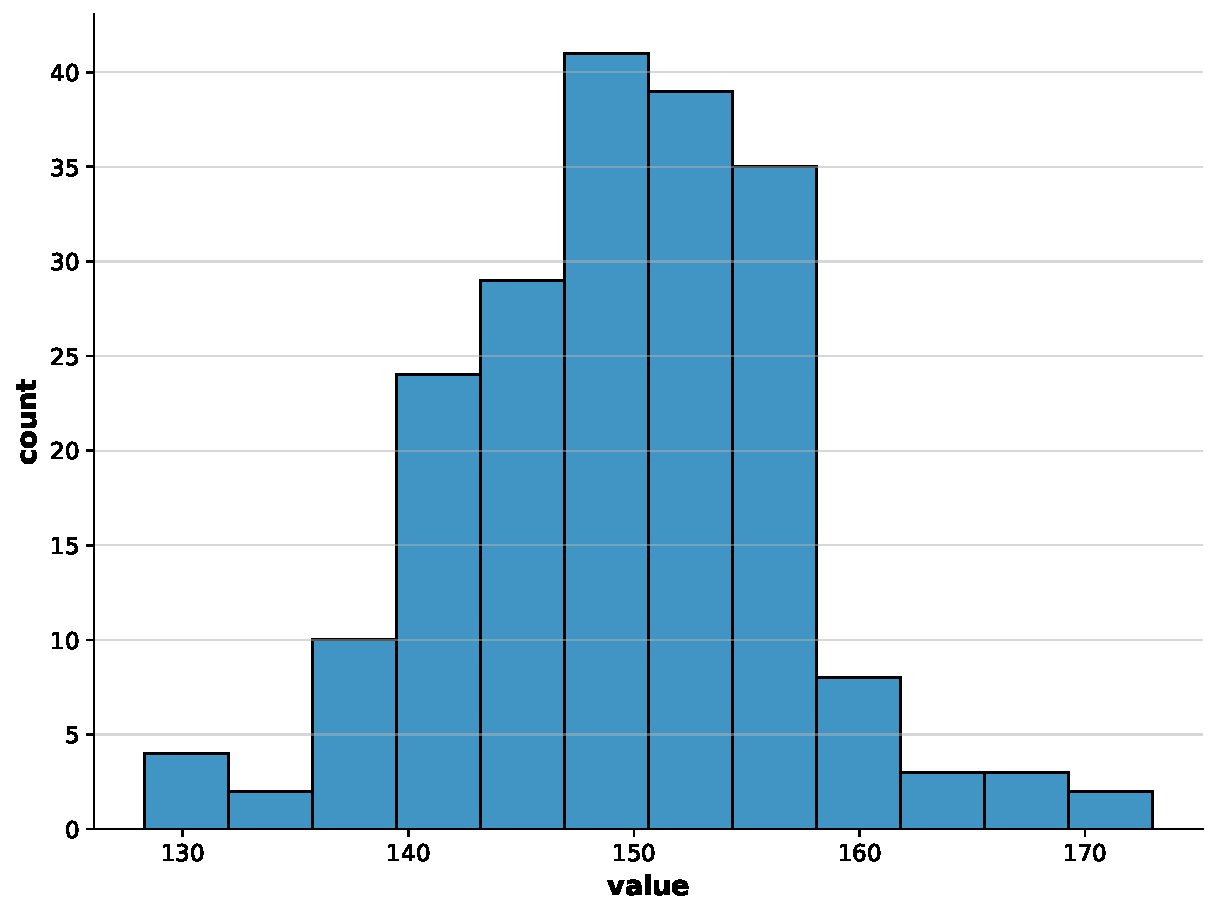
\includegraphics[width=0.48\textwidth,height=0.36\textheight,keepaspectratio]{figures/lesson13_example2_lesson13_heights.pdf}
\captionof{figure}{Lesson 13, example 2: \code{lesson13\_\allowbreak{}line.\allowbreak{}png} and \code{lesson13\_\allowbreak{}heights.\allowbreak{}png}.}
\end{minipage}\end{center}
\section*{Example 3}
A grid holds numbers in rows and columns. Positions count from 1.
\begin{lstlisting}[style=py]
import simplydata as sdata
grid = sdata.number_grid([[3, 5, 2], [8, 6, 4]])
print(grid.number_at(row=1, column=2))
grid.total(for_each="row")
grid.average(for_each="column")
grid.swap_rows_and_columns()
print(grid)
chart = grid.chart()
chart.heatmap(numbers=True)
chart.save("lesson13_grid.png")
\end{lstlisting}
\whateachline
\begin{lineexplain}
  \item[1] Load simplydata.
  \item[2] A grid with 2 rows and 3 columns: one list for each row.
  \item[3] The number in row 1, column 2: 5.
  \item[4] The total of each row: 10 and 18.
  \item[5] The average of each column.
  \item[6] Rows become columns (in maths: the transpose).
  \item[7] Now 3 rows and 2 columns.
  \item[8] Start a chart from the grid.
  \item[9] One coloured square for each number, with the number written in.
  \item[10] Save it.
\end{lineexplain}
\printedoutput{output/lesson13_example3.txt}
\begin{center}\begin{minipage}{\linewidth}\centering
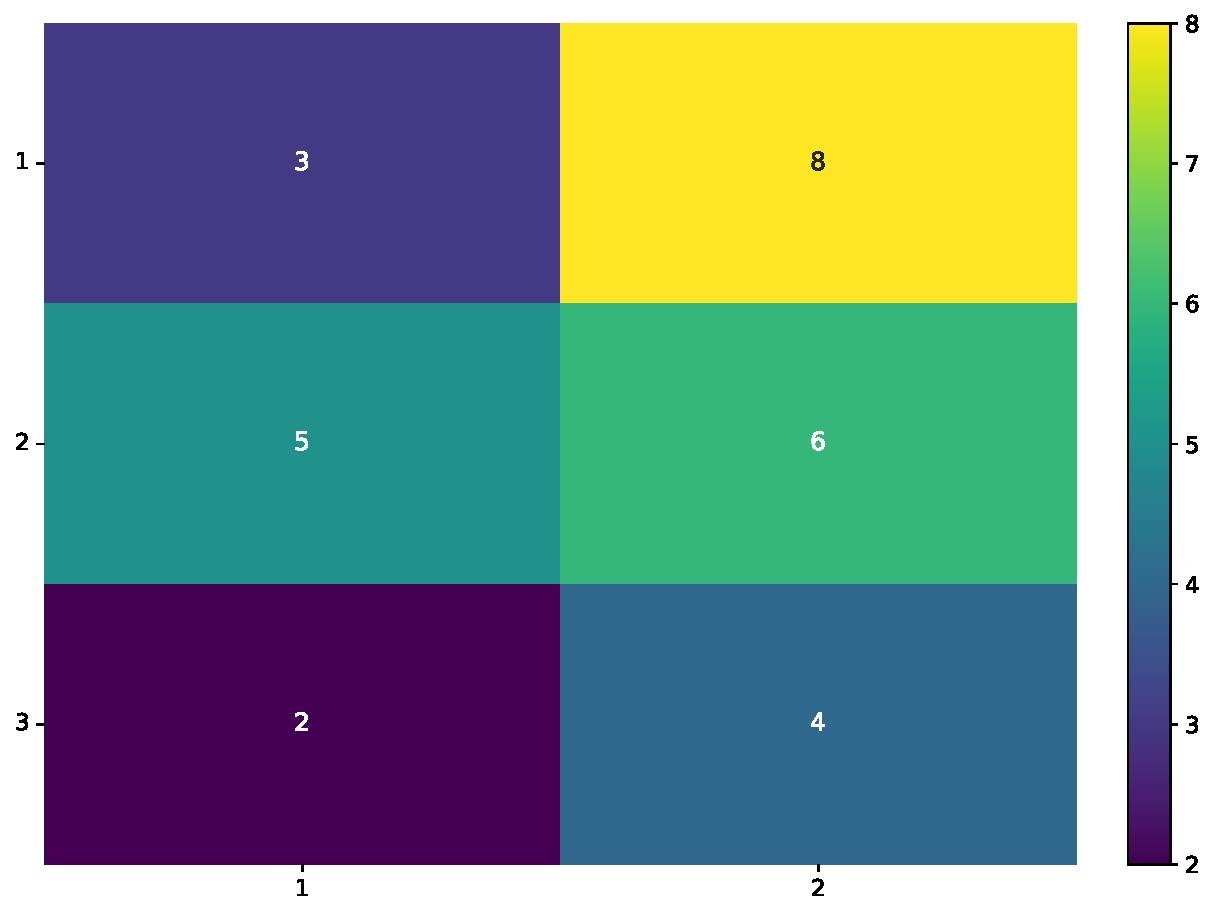
\includegraphics[width=0.72\textwidth,height=0.36\textheight,keepaspectratio]{figures/lesson13_example3_lesson13_grid.pdf}
\captionof{figure}{Lesson 13, example 3: \code{lesson13\_\allowbreak{}grid.\allowbreak{}png}.}
\end{minipage}\end{center}
\begin{goodtoknow}
\begin{itemize}
  \item The words follow the table words, with numbers in place of rows: \code{keep\_\allowbreak{}first\_\allowbreak{}numbers}, \code{remove\_\allowbreak{}empty\_\allowbreak{}numbers}, \code{fill\_\allowbreak{}empty\_\allowbreak{}numbers}, \code{show\_\allowbreak{}first\_\allowbreak{}numbers}.
  \item Summaries have no \_of, because there is no column to name: \code{nums.\allowbreak{}average()}, not \code{table.\allowbreak{}average\_\allowbreak{}of(\textquotedbl{}marks\textquotedbl{})}.
  \item A sum with no answer, such as dividing by 0 or the square root of a negative number, gives an empty value and a note, never a crash.
  \item \code{nums.\allowbreak{}table()} turns numbers into a table, and \code{nums.\allowbreak{}as\_\allowbreak{}numpy()} gives a plain NumPy array if another Python tool needs one.
\end{itemize}
\end{goodtoknow}
\begin{tryit}
\begin{enumerate}
  \item Make the numbers 1 to 10, then square them in two ways: with ** 2 and with \code{power(2)}.
  \item Make 6 dice throws with \code{sdata.\allowbreak{}random\_\allowbreak{}numbers(how\_\allowbreak{}many=6,\allowbreak{} between=[1,\allowbreak{} 6],\allowbreak{} whole\_\allowbreak{}numbers=True,\allowbreak{} seed=1)}. What is their total?
  \item Make a grid of 3 rows and 4 columns filled with 0: \code{sdata.\allowbreak{}number\_\allowbreak{}grid(rows=3,\allowbreak{} columns=4,\allowbreak{} filled\_\allowbreak{}with=0)}.
\end{enumerate}
Worked solutions: page~\pageref{solutions:13}, or type \code{sdata.\allowbreak{}lesson(13,\allowbreak{} solutions=True)}.
\end{tryit}
\par\noindent{\small\sffamily\textbf{Words in this lesson:} \hyperref[word:sdata.numbers]{\code{sdata.\allowbreak{}numbers()}}, \hyperref[word:sdata.random-numbers]{\code{sdata.\allowbreak{}random\_\allowbreak{}numbers()}}, \hyperref[word:sdata.number-grid]{\code{sdata.\allowbreak{}number\_\allowbreak{}grid()}}, \hyperref[word:nums.add]{\code{nums.\allowbreak{}add()}}, \hyperref[word:nums.undo]{\code{nums.\allowbreak{}undo()}}, \hyperref[word:nums.keep-numbers]{\code{nums.\allowbreak{}keep\_\allowbreak{}numbers()}}, \hyperref[word:nums.average]{\code{nums.\allowbreak{}average()}}, \hyperref[word:nums.standard-deviation]{\code{nums.\allowbreak{}standard\_\allowbreak{}deviation()}}, \hyperref[word:nums.median]{\code{nums.\allowbreak{}median()}}, \hyperref[word:nums.percentile]{\code{nums.\allowbreak{}percentile()}}, \hyperref[word:nums.chart]{\code{nums.\allowbreak{}chart()}}, \hyperref[word:grid.number-at]{\code{grid.\allowbreak{}number\_\allowbreak{}at()}}, \hyperref[word:grid.swap-rows-and-columns]{\code{grid.\allowbreak{}swap\_\allowbreak{}rows\_\allowbreak{}and\_\allowbreak{}columns()}}, \hyperref[word:nums.steps]{\code{nums.\allowbreak{}steps()}}.\par}

\chapter{Statistical tests: real difference, or chance?}\label{lesson:14}
\begin{learnbox}
\begin{itemize}
  \item what a statistical test asks, and what a p-value means
  \item how to compare the averages of groups, and which groups differ
  \item how to compare counts, and how to fit a line or a formula
\end{itemize}
\end{learnbox}
\section*{Example 1}
Groups almost never have exactly the same average. A test asks: is the difference bigger than chance alone would often give?
\begin{lstlisting}[style=py]
import simplydata as sdata
table = sdata.table(sdata.example("marks"))
table.compare_averages("marks", for_each="class")
table.compare_each_pair("marks", for_each="class")
table.compare_averages("marks", for_each="subject", based_on="ranks")
\end{lstlisting}
\whateachline
\begin{lineexplain}
  \item[1] Load simplydata.
  \item[2] Make a table of the marks.
  \item[3] Do the three classes really differ in their average mark? The answer comes in words. The p-value is the chance of a difference this big if the classes were really the same: below 0.05 we call it unlikely to be chance. With three or more groups this test is also called Welch's ANOVA; with two groups, a t-test.
  \item[4] Which classes differ? Each pair gets its own t-test (Welch's). Testing many pairs makes a false alarm more likely, so the p-values are adjusted (Holm's method).
  \item[5] \code{based\_\allowbreak{}on=\textquotedbl{}ranks\textquotedbl{}} puts the marks in order and compares the places instead (a Kruskal-Wallis test, or Mann-Whitney for two groups). It is safer when groups are small and the values are not bell-shaped.
\end{lineexplain}
\printedoutput{output/lesson14_example1.txt}
\section*{Example 2}
Counts can be compared too: does how often something happens differ between groups?
\begin{lstlisting}[style=py]
import simplydata as sdata
table = sdata.table(sdata.example("marks"))
table.add_group_column("result", from_column="marks", cut_at=[60], names=["below 60", "60 or more"])
table.compare_counts("result", for_each="class")
\end{lstlisting}
\whateachline
\begin{lineexplain}
  \item[1] Load simplydata.
  \item[2] Make a table of the marks.
  \item[3] A new column that says if each mark is below 60 or not.
  \item[4] Do the classes differ in how many marks are 60 or more? This counts the rows for each class and result and uses the chi-square test. Cramer's V says how strong the link is, from 0 (none) to 1.
\end{lineexplain}
\printedoutput{output/lesson14_example2.txt}
\section*{Example 3}
A fit finds the line or formula that follows the data best, and says how sure it is.
\begin{lstlisting}[style=py]
import simplydata as sdata
table = sdata.table(sdata.example("marks"))
table.fit_line(x="hours", y="marks")
growth = sdata.table(sdata.example("growth"))
growth.keep_rows("country", equal_to="Applia")
growth.fit_formula("population = a * exp(b * (year - 2000))")
\end{lstlisting}
\whateachline
\begin{lineexplain}
  \item[1] Load simplydata.
  \item[2] Make a table of the marks.
  \item[3] How much do the marks go up for each extra hour of study? This is linear regression by least squares. R squared says how much of the differences in marks the line explains.
  \item[4] A second table, with the growth data.
  \item[5] Keep one country.
  \item[6] Fit a formula you write yourself. Names that are columns (population, year) are data; the others (a and b) are found by simplydata. Here b is the growth rate each year. This is nonlinear least squares.
\end{lineexplain}
\printedoutput{output/lesson14_example3.txt}
\section*{Example 4}
Before a test, look at the shape of the values and at values far from the rest. After many tests, adjust the p-values.
\begin{lstlisting}[style=py]
import simplydata as sdata
table = sdata.table(sdata.example("marks"))
table.compare_shape_to("marks", "normal", for_each="class")
table.show_rows_with_outliers("marks", for_each="class")
pairs = table.correlation_between("hours", "marks", "height", show="each pair")
pairs.add_adjusted_p_value_column(method="holm")
pairs.show()
\end{lstlisting}
\whateachline
\begin{lineexplain}
  \item[1] Load simplydata.
  \item[2] Make a table of the marks.
  \item[3] Do the marks of each class look bell-shaped (normal)? The Shapiro-Wilk test answers for each class. Tests on averages work best with bell-shaped values, or with many values.
  \item[4] The rows whose mark is far from the rest of its class, by Tukey's rule (the one box plots use): here one mark of 33 in class B. The table does not change.
  \item[5] Test three pairs of columns at once: a table with one row per pair and its p-value.
  \item[6] With many tests, one of them looks real by chance more often. Holm's adjustment keeps the chance of even one false alarm at 5 \%.
  \item[7] The p-values and the adjusted ones, side by side.
\end{lineexplain}
\printedoutput{output/lesson14_example4.txt}
\section*{Example 5}
Some questions are about spread, or about counts compared with what you expect.
\begin{lstlisting}[style=py]
import simplydata as sdata
table = sdata.table(sdata.example("marks"))
table.compare_spreads("marks", for_each="class")
table.compare_each_pair("marks", for_each="class", test="tukey")
school = sdata.table(sdata.example("school"))
school.compare_counts_to("breakfast", expected={"yes": 0.6, "no": 0.4})
school.compare_percent_to("passed", value="yes", percent=50)
\end{lstlisting}
\whateachline
\begin{lineexplain}
  \item[1] Load simplydata.
  \item[2] Make a table of the marks.
  \item[3] Are the marks of one class more spread out? Levene's test says this could easily be chance (p = 0.91).
  \item[4] Tukey's test compares every pair at once: only A and C differ (p = 0.020).
  \item[5] A table of pupils.
  \item[6] Did 60 \% eat breakfast, as a survey said? 115 of 180 is close enough (p = 0.29).
  \item[7] Did half the pupils pass? 43.3 \% did; that could easily be chance (p = 0.086).
\end{lineexplain}
\printedoutput{output/lesson14_example5.txt}
\begin{goodtoknow}
\begin{itemize}
  \item The idea behind every test: imagine there is no real difference (this is called the null hypothesis). The p-value says how surprising your data would be then. A small p-value means: hard to explain by chance alone.
  \item A p-value does not say how big or important the difference is: the effect size does that (omega-squared, Cohen's d, Cramer's V ...). And a large p-value does not show that there is no difference. It only means these data cannot tell.
  \item A 95 \% confidence interval is the range the true value is very likely in. A narrow one means the data pin the value down well; a wide one means you need more data.
  \item Each test gives back a one-row table with all its numbers, so you can save it: result = \code{table.\allowbreak{}compare\_\allowbreak{}averages(.\allowbreak{}.\allowbreak{}.\allowbreak{})}, then \code{result.\allowbreak{}save(\textquotedbl{}test.\allowbreak{}csv\textquotedbl{})}.
  \item Also: \code{compare\_\allowbreak{}before\_\allowbreak{}after} for two measurements of the same thing (a paired t-test), and \code{compare\_\allowbreak{}average\_\allowbreak{}to} for one average against a number you choose.
  \item \code{remove\_\allowbreak{}rows\_\allowbreak{}with\_\allowbreak{}outliers} removes such rows. Say in your report which rule removed how many rows, and never remove a value only because it spoils the result.
  \item \code{method=\textquotedbl{}benjamini-hochberg\textquotedbl{}} adjusts for many tests more gently: it controls the share of false alarms among your findings (the false discovery rate).
\end{itemize}
\end{goodtoknow}
\begin{tryit}
\begin{enumerate}
  \item Compare the average marks \code{for\_\allowbreak{}each=\textquotedbl{}subject\textquotedbl{}}. Could the differences be chance?
  \item Is the average temperature different between the cities of \code{sdata.\allowbreak{}example(\textquotedbl{}weather\textquotedbl{})}?
  \item Fit a straight line of \code{\textquotedbl{}forest\textquotedbl{}} against \code{\textquotedbl{}year\textquotedbl{}} in \code{sdata.\allowbreak{}example(\textquotedbl{}growth\textquotedbl{})} for one country.
  \item Remove the rows with outliers in \code{\textquotedbl{}marks\textquotedbl{}} \code{for\_\allowbreak{}each=\textquotedbl{}class\textquotedbl{}}, then compare the average marks \code{for\_\allowbreak{}each=\textquotedbl{}class\textquotedbl{}} again. Did the answer change?
\end{enumerate}
Worked solutions: page~\pageref{solutions:14}, or type \code{sdata.\allowbreak{}lesson(14,\allowbreak{} solutions=True)}.
\end{tryit}
\par\noindent{\small\sffamily\textbf{Words in this lesson:} \hyperref[word:table.compare-averages]{\code{table.\allowbreak{}compare\_\allowbreak{}averages()}}, \hyperref[word:table.compare-each-pair]{\code{table.\allowbreak{}compare\_\allowbreak{}each\_\allowbreak{}pair()}}, \hyperref[word:table.compare-counts]{\code{table.\allowbreak{}compare\_\allowbreak{}counts()}}, \hyperref[word:table.fit-line]{\code{table.\allowbreak{}fit\_\allowbreak{}line()}}, \hyperref[word:table.fit-formula]{\code{table.\allowbreak{}fit\_\allowbreak{}formula()}}, \hyperref[word:table.add-group-column]{\code{table.\allowbreak{}add\_\allowbreak{}group\_\allowbreak{}column()}}, \hyperref[word:table.compare-shape-to]{\code{table.\allowbreak{}compare\_\allowbreak{}shape\_\allowbreak{}to()}}, \hyperref[word:table.show-rows-with-outliers]{\code{table.\allowbreak{}show\_\allowbreak{}rows\_\allowbreak{}with\_\allowbreak{}outliers()}}, \hyperref[word:table.add-adjusted-p-value-column]{\code{table.\allowbreak{}add\_\allowbreak{}adjusted\_\allowbreak{}p\_\allowbreak{}value\_\allowbreak{}column()}}, \hyperref[word:table.remove-rows-with-outliers]{\code{table.\allowbreak{}remove\_\allowbreak{}rows\_\allowbreak{}with\_\allowbreak{}outliers()}}, \hyperref[word:table.compare-spreads]{\code{table.\allowbreak{}compare\_\allowbreak{}spreads()}}, \hyperref[word:table.compare-counts-to]{\code{table.\allowbreak{}compare\_\allowbreak{}counts\_\allowbreak{}to()}}, \hyperref[word:table.compare-percent-to]{\code{table.\allowbreak{}compare\_\allowbreak{}percent\_\allowbreak{}to()}}.\par}

\chapter{A whole analysis: from a question to a figure}\label{lesson:15}
\begin{learnbox}
\begin{itemize}
  \item how to put all the lessons together: open, look, clean, sum up, test, draw and save
  \item how to make a figure with panels A and B, ready for a report or a paper
  \item how \code{steps()} writes down what you did, in plain words
  \item how to hand your table to pandas or Polars, and back
\end{itemize}
\end{learnbox}
\section*{Example 1}
A whole analysis with one question: do children who study longer get better marks, and do the classes differ? One table feeds two charts, and the two charts become one figure.
\begin{lstlisting}[style=py]
import simplydata as sdata
table = sdata.table(sdata.example("marks"))
table.describe_columns()
table.remove_rows_with_empty_cells()
table.average_of("marks", for_each="class")
table.compare_averages("marks", for_each="class")
a = table.chart()
a.boxes(x="class", y="marks")
a.all_dots(x="class", y="marks")
a.label_y("Mark (out of 100)")
b = table.chart()
b.dots(x="hours", y="marks", colour="class")
b.fit_line(confidence_band=True)
b.label_x("Hours of study")
figure = sdata.grid(a, b, per_row=2, letters=True)
figure.title_top("Marks, classes and hours of study")
figure.style("paper")
figure.size(width=17, height=8, unit="cm")
figure.save("lesson15_figure.pdf")
figure.save("lesson15_figure.tif", resolution=600)
table.save("lesson15_clean.xlsx")
table.steps()
\end{lstlisting}
\whateachline
\begin{lineexplain}
  \item[1] Load simplydata.
  \item[2] Open the data. For your own file: \code{sdata.\allowbreak{}table(\textquotedbl{}results.\allowbreak{}xlsx\textquotedbl{})}.
  \item[3] Look: what is in each column, and are any cells empty?
  \item[4] Clean: remove the rows with an empty cell. The practice table has none, so nothing is removed.
  \item[5] Sum up: the average mark of each class.
  \item[6] Test: could the differences between the classes be chance?
  \item[7] Chart A, from the cleaned table.
  \item[8] The marks of each class as boxes.
  \item[9] Every mark as a dot, on top of the boxes.
  \item[10] Name its y-axis.
  \item[11] Chart B, from the same table.
  \item[12] Hours of study against marks, one colour per class.
  \item[13] A straight line for each class, with its 95 \% confidence band.
  \item[14] Name its x-axis.
  \item[15] Both charts on one page, with A and B at the top left.
  \item[16] A title for the whole page.
  \item[17] A quiet look that suits a paper.
  \item[18] The size a journal asks for: 17 cm wide (a full page width) and 8 cm high.
  \item[19] Save the figure as a PDF: sharp at any size.
  \item[20] And as a \code{.\allowbreak{}tif} picture with 600 dots per inch, as many journals ask.
  \item[21] Save the cleaned table that the figure was drawn from.
  \item[22] Every table step in plain words, in order: a good start for the methods part of your report.
\end{lineexplain}
\printedoutput{output/lesson15_example1.txt}
\begin{center}\begin{minipage}{\linewidth}\centering
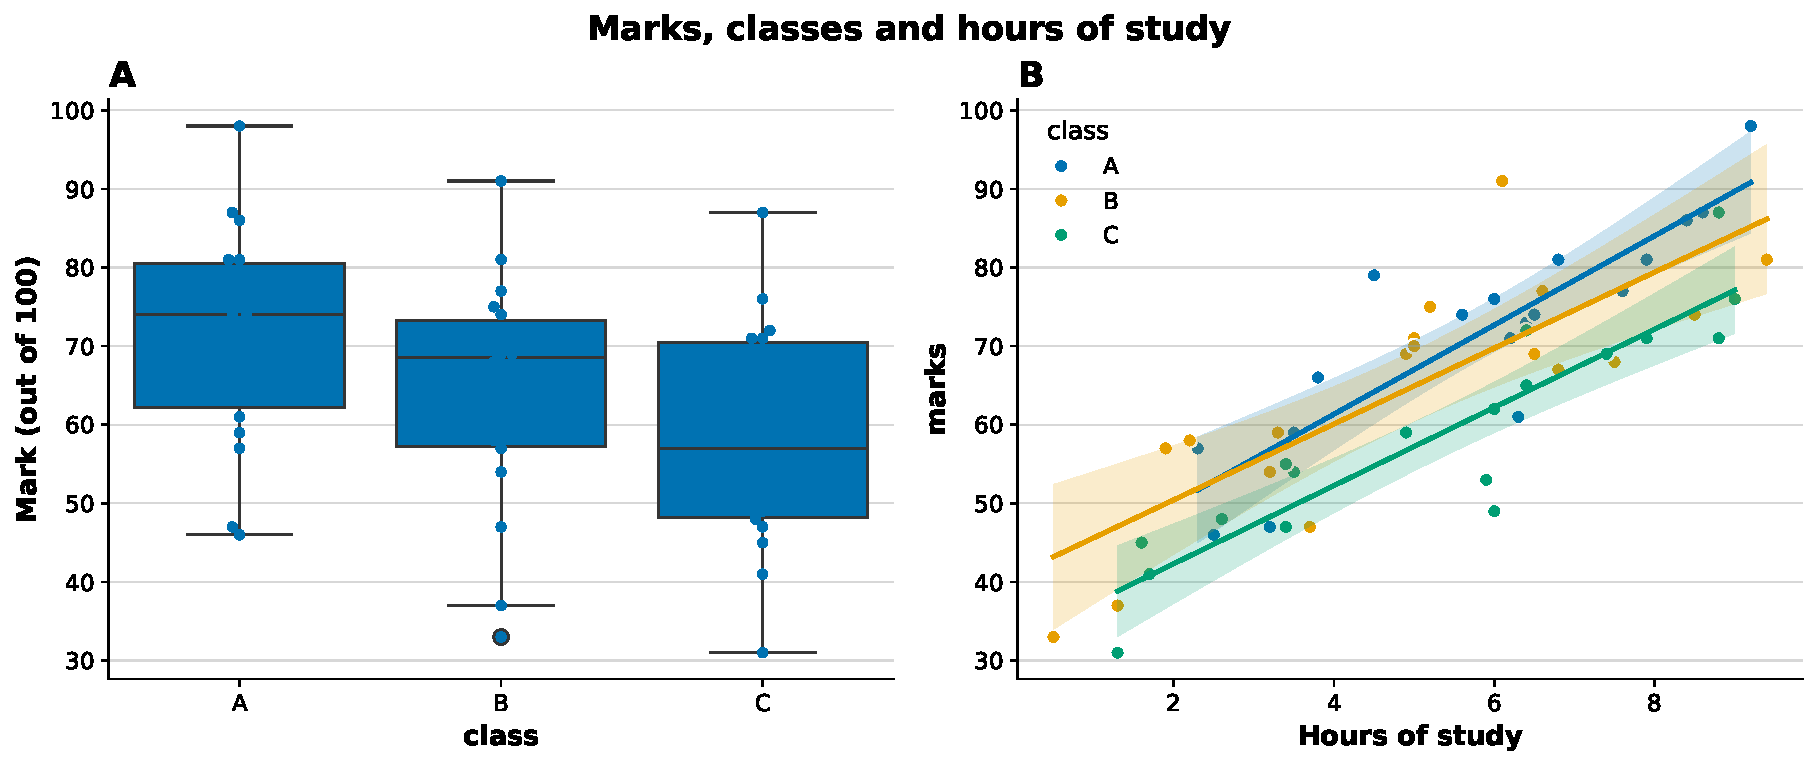
\includegraphics[width=0.72\textwidth,height=0.36\textheight,keepaspectratio]{figures/lesson15_example1_lesson15_figure.pdf}
\captionof{figure}{Lesson 15, example 1: \code{lesson15\_\allowbreak{}figure.\allowbreak{}pdf}.}
\end{minipage}\end{center}
\section*{Example 2}
Two questions about two tables give two charts. \code{sdata.\allowbreak{}grid} puts them on one page.
\begin{lstlisting}[style=py]
import simplydata as sdata
weather = sdata.table(sdata.example("weather"))
weather.keep_rows("city", equal_to="Rainbridge")
rain = weather.chart()
rain.bars(x="month", y="rain")
rain.line_at_y(100, label="100 mm")
growth = sdata.table(sdata.example("growth"))
forest = growth.chart()
forest.lines(x="year", y="forest", colour="country")
forest.label_y("Forest (% of the land)")
page = sdata.grid(rain, forest, per_row=2, letters=True)
page.save("lesson15_two_tables.png")
\end{lstlisting}
\whateachline
\begin{lineexplain}
  \item[1] Load simplydata.
  \item[2] Table 1: the weather.
  \item[3] Keep one city.
  \item[4] A chart of it, called rain.
  \item[5] Its rain through the year.
  \item[6] A line at 100 mm.
  \item[7] Table 2: four countries.
  \item[8] A chart of it, called forest.
  \item[9] Their forest over the years.
  \item[10] Name the y-axis.
  \item[11] Both charts on one page, with letters.
  \item[12] Save the page.
\end{lineexplain}
\printedoutput{output/lesson15_example2.txt}
\begin{center}\begin{minipage}{\linewidth}\centering
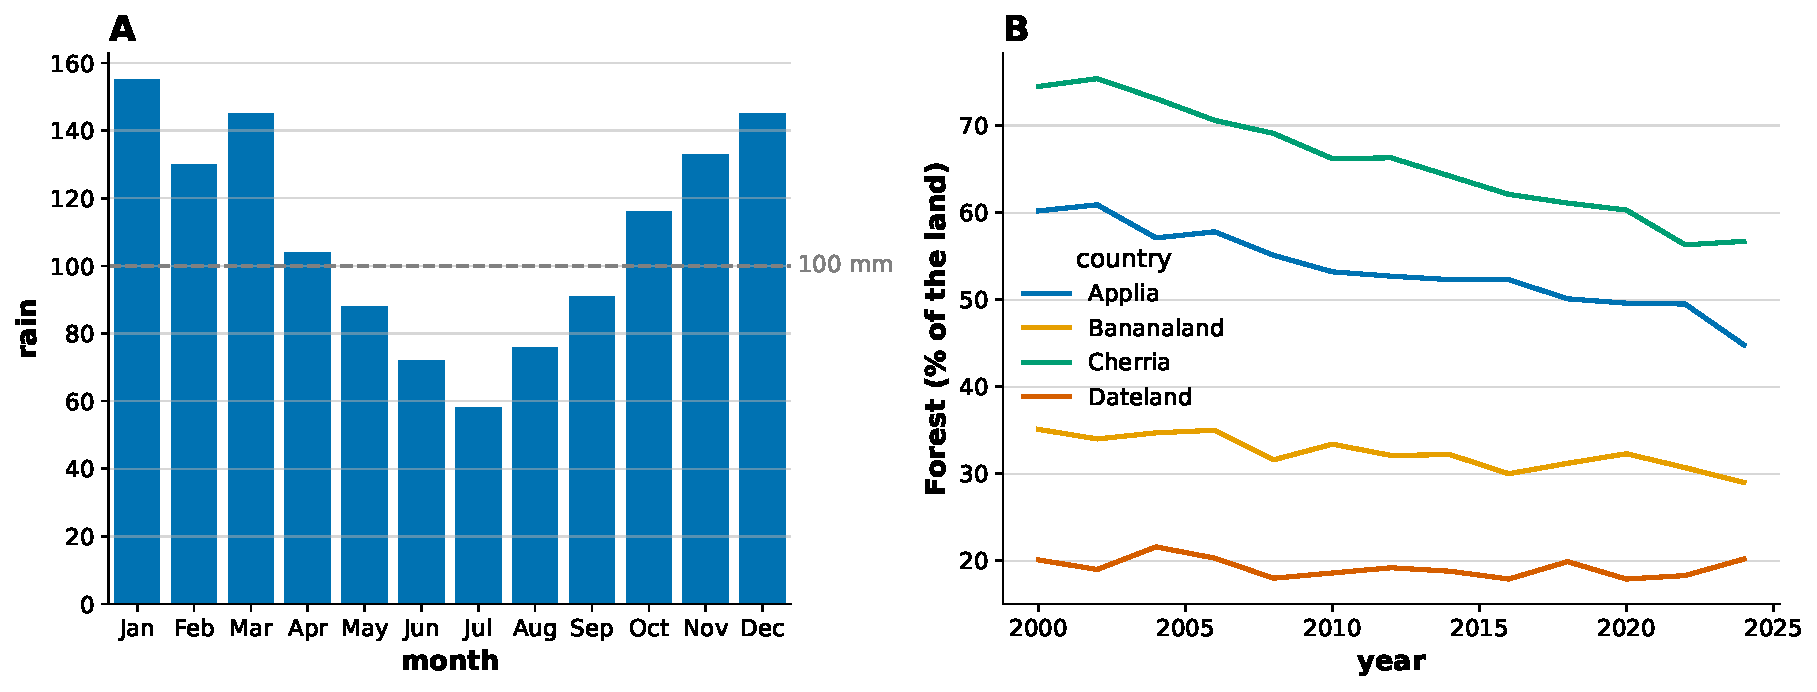
\includegraphics[width=0.72\textwidth,height=0.36\textheight,keepaspectratio]{figures/lesson15_example2_lesson15_two_tables.pdf}
\captionof{figure}{Lesson 15, example 2: \code{lesson15\_\allowbreak{}two\_\allowbreak{}tables.\allowbreak{}png}.}
\end{minipage}\end{center}
\section*{Example 3}
A table goes to pandas or Polars and back whenever another Python tool needs it.
\begin{lstlisting}[style=py]
import simplydata as sdata
table = sdata.table(sdata.example("weather"))
table.keep_rows("city", equal_to="Rainbridge")
df = table.as_pandas()
print(df["rain"].max())
again = sdata.table(df)
chart = sdata.chart(df)
chart.bars(x="month", y="rain")
chart.save("lesson15_rain.png")
\end{lstlisting}
\whateachline
\begin{lineexplain}
  \item[1] Load simplydata.
  \item[2] A table of the weather.
  \item[3] Keep one city.
  \item[4] A plain pandas DataFrame (\code{table.\allowbreak{}as\_\allowbreak{}polars()} gives a Polars one).
  \item[5] Any pandas code works on it.
  \item[6] And back: \code{sdata.\allowbreak{}table} takes a pandas or Polars table you already have.
  \item[7] \code{sdata.\allowbreak{}chart} takes one too.
  \item[8] Draw it.
  \item[9] Save the chart.
\end{lineexplain}
\printedoutput{output/lesson15_example3.txt}
\begin{center}\begin{minipage}{\linewidth}\centering
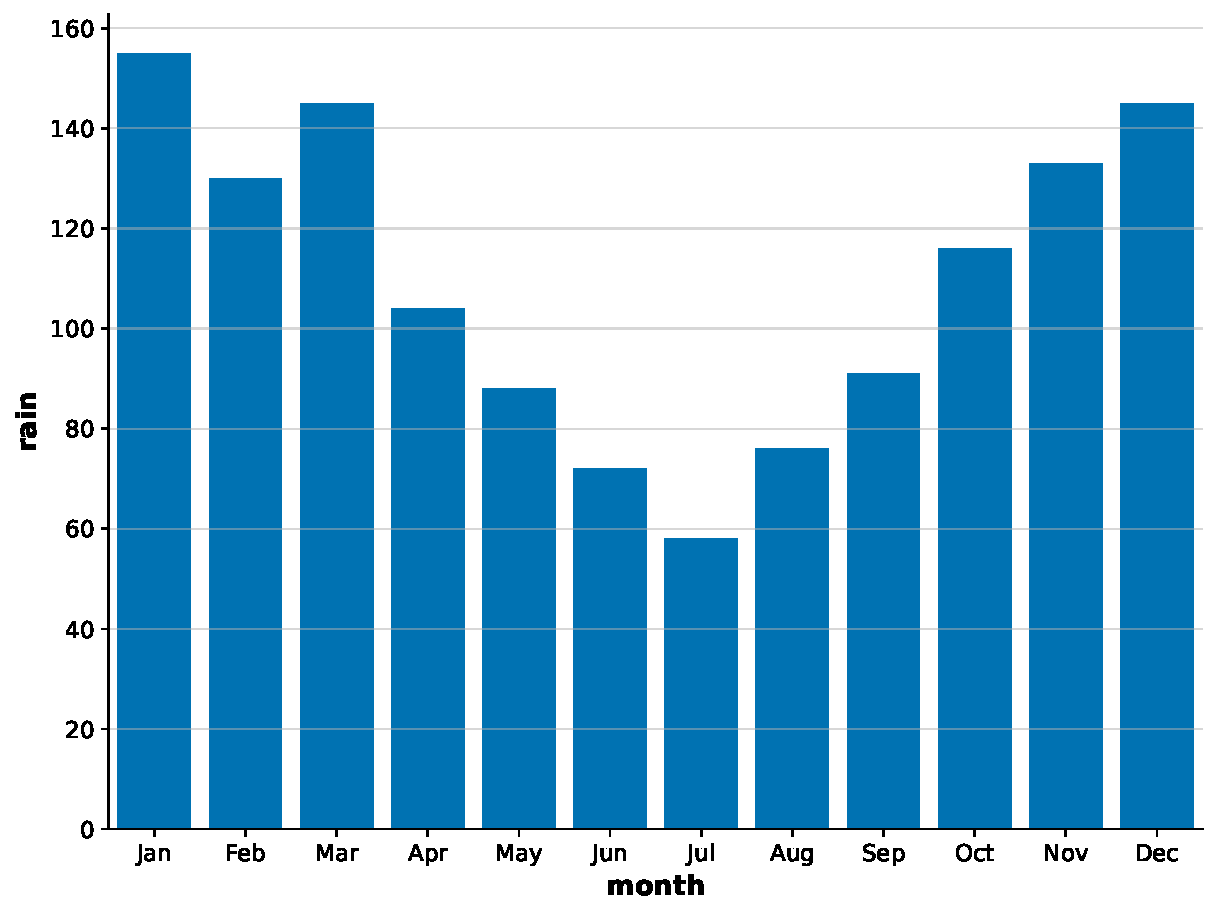
\includegraphics[width=0.72\textwidth,height=0.36\textheight,keepaspectratio]{figures/lesson15_example3_lesson15_rain.pdf}
\captionof{figure}{Lesson 15, example 3: \code{lesson15\_\allowbreak{}rain.\allowbreak{}png}.}
\end{minipage}\end{center}
\begin{goodtoknow}
\begin{itemize}
  \item Every analysis follows the same plan: open, look, clean, sum up, test, draw, words, save. Lessons 1 to 14 taught each part; this lesson puts them together.
  \item The table and the charts are separate objects, as in pandas and matplotlib: one cleaned table can feed many charts, and each chart keeps the rows the table had when the chart was made.
  \item \code{table.\allowbreak{}save} saves the table, and \code{chart.\allowbreak{}save} or \code{page.\allowbreak{}save} the picture. Save both, so anyone can check the figure against its data.
  \item \code{table.\allowbreak{}steps()} lists the table steps. Together with the chart lines of your program, it says everything you did.
  \item simplydata words never need \code{as\_\allowbreak{}pandas()}; it is only for other tools.
\end{itemize}
\end{goodtoknow}
\begin{tryit}
\begin{enumerate}
  \item Do a whole analysis of \code{sdata.\allowbreak{}example(\textquotedbl{}weather\textquotedbl{})}: look at it, compare the average rain \code{for\_\allowbreak{}each=\textquotedbl{}city\textquotedbl{}}, draw the rain of each city as boxes, and save the chart and the table.
  \item Make a second chart of the temperature, then put the two charts together with \code{sdata.\allowbreak{}side\_\allowbreak{}by\_\allowbreak{}side(.\allowbreak{}.\allowbreak{}.\allowbreak{},\allowbreak{} letters=True)}.
  \item Read the \code{steps()} of your table out loud. Would someone else understand what you did?
\end{enumerate}
Worked solutions: page~\pageref{solutions:15}, or type \code{sdata.\allowbreak{}lesson(15,\allowbreak{} solutions=True)}.
\end{tryit}
\par\noindent{\small\sffamily\textbf{Words in this lesson:} \hyperref[word:sdata.table]{\code{sdata.\allowbreak{}table()}}, \hyperref[word:table.describe-columns]{\code{table.\allowbreak{}describe\_\allowbreak{}columns()}}, \hyperref[word:table.remove-rows-with-empty-cells]{\code{table.\allowbreak{}remove\_\allowbreak{}rows\_\allowbreak{}with\_\allowbreak{}empty\_\allowbreak{}cells()}}, \hyperref[word:table.compare-averages]{\code{table.\allowbreak{}compare\_\allowbreak{}averages()}}, \hyperref[word:table.chart]{\code{table.\allowbreak{}chart()}}, \hyperref[word:boxes]{\code{chart.\allowbreak{}boxes()}}, \hyperref[word:all-dots]{\code{chart.\allowbreak{}all\_\allowbreak{}dots()}}, \hyperref[word:dots]{\code{chart.\allowbreak{}dots()}}, \hyperref[word:fit-line]{\code{chart.\allowbreak{}fit\_\allowbreak{}line()}}, \hyperref[word:sdata.grid]{\code{sdata.\allowbreak{}grid()}}, \hyperref[word:style]{\code{chart.\allowbreak{}style()}}, \hyperref[word:table.save]{\code{table.\allowbreak{}save()}}, \hyperref[word:table.steps]{\code{table.\allowbreak{}steps()}}, \hyperref[word:table.as-pandas]{\code{table.\allowbreak{}as\_\allowbreak{}pandas()}}, \hyperref[word:sdata.chart]{\code{sdata.\allowbreak{}chart()}}.\par}

\chapter{Models: explain one column from several others}\label{lesson:16}
\begin{learnbox}
\begin{itemize}
  \item how to explain one column from several others at once (multiple regression)
  \item how to explain a yes/no column (logistic regression) and a column of counts (Poisson regression)
  \item how to allow for groups such as schools (a mixed model)
  \item how to use rows with empty cells without guessing once (multiple imputation)
\end{itemize}
\end{learnbox}
\section*{Example 1}
Marks depend on more than one thing. \code{explain()} looks at several columns together, so each effect is the effect with the other columns held fixed.
\begin{lstlisting}[style=py]
import simplydata as sdata
table = sdata.table(sdata.example("school"))
table.explain("marks", using=["hours", "sleep", "breakfast"])
table.explain("marks", using=["hours * breakfast"])
\end{lstlisting}
\whateachline
\begin{lineexplain}
  \item[1] Load simplydata.
  \item[2] Pupils in 12 schools: study, sleep, breakfast and marks.
  \item[3] Explain the marks from hours of study, hours of sleep and breakfast. Each extra hour of study goes with about 2.7 more marks, each extra hour of sleep with 2.3 more, and breakfast with 3.2 more, each with its 95 \% confidence interval and p-value. This is a linear model (multiple regression) by least squares.
  \item[4] hours * breakfast also asks: does the effect of study depend on breakfast? That is an interaction. Here it could easily be chance (p = 0.31).
\end{lineexplain}
\printedoutput{output/lesson16_example1.txt}
\section*{Example 2}
Not every column is a number to explain. A yes/no column needs the chance of yes, and a count needs a model for counts.
\begin{lstlisting}[style=py]
import simplydata as sdata
table = sdata.table(sdata.example("school"))
table.explain("passed", using=["hours", "breakfast"], outcome="yes or no")
table.explain("days_absent", using=["hours", "sleep"], outcome="counts")
table.add_predicted_column("marks", using=["hours", "breakfast"])
table.show_first_rows(5)
\end{lstlisting}
\whateachline
\begin{lineexplain}
  \item[1] Load simplydata.
  \item[2] The school table.
  \item[3] Did the pupil pass? \code{outcome=\textquotedbl{}yes or no\textquotedbl{}} is logistic regression. Each extra hour of study multiplies the odds of passing by 1.66 (an odds ratio).
  \item[4] Days absent are counts (0, 1, 2 ...). \code{outcome=\textquotedbl{}counts\textquotedbl{}} is Poisson regression; each extra hour of study multiplies the expected days absent by 0.88 (a rate ratio).
  \item[5] Add a column \code{\textquotedbl{}predicted marks\textquotedbl{}}: what the model expects for each pupil.
  \item[6] Look at the marks next to the predicted marks.
\end{lineexplain}
\printedoutput{output/lesson16_example2.txt}
\section*{Example 3}
Pupils in the same school are alike in ways the columns do not show. A mixed model allows for that, and multiple imputation uses the rows with empty cells.
\begin{lstlisting}[style=py]
import simplydata as sdata
table = sdata.table(sdata.example("school"))
table.explain("marks", using=["hours", "breakfast"], grouped_by="school")
table.explain("marks", using=["hours", "sleep", "breakfast"], empty_cells="multiple imputation")
\end{lstlisting}
\whateachline
\begin{lineexplain}
  \item[1] Load simplydata.
  \item[2] The school table.
  \item[3] A mixed model: each school gets its own starting level (a random intercept). About 39 \% of the differences the columns do not explain lie between schools (the ICC).
  \item[4] 19 pupils did not say how long they slept. Instead of leaving them out, multiple imputation fills the empty cells 20 times, fits the model to each filled-in table and pools the 20 answers (Rubin's rules), so the extra uncertainty is counted.
\end{lineexplain}
\printedoutput{output/lesson16_example3.txt}
\begin{goodtoknow}
\begin{itemize}
  \item Each effect in \code{explain()} holds the other columns fixed: the effect of sleep is the effect for pupils who study the same number of hours and have the same breakfast.
  \item A text column such as breakfast is compared with its first group in A to Z order (here \code{\textquotedbl{}no\textquotedbl{}}); the answer says which group is the baseline.
  \item An odds ratio above 1 means higher odds of yes; a rate ratio above 1 means more counts. 1 means no difference.
  \item If counts vary much more than a Poisson model expects (overdispersion), simplydata says so and suggests \code{outcome=\textquotedbl{}counts (overdispersed)\textquotedbl{}}; it never switches by itself.
  \item \code{grouped\_\allowbreak{}by=} is for rows that come in groups: pupils in schools, measurements on the same animal, samples from the same site. Without it, the p-values are too small.
  \item Multiple imputation needs the empty cells to be explainable by the other columns (missing at random). Say in your report how many cells were empty and how they were handled.
  \item \code{grouped\_\allowbreak{}by=} and multiple imputation need the statsmodels package: pip install \code{\textquotedbl{}simplydata[stats]\textquotedbl{}}.
\end{itemize}
\end{goodtoknow}
\begin{tryit}
\begin{enumerate}
  \item Explain \code{\textquotedbl{}marks\textquotedbl{}} using \code{\textquotedbl{}hours\textquotedbl{}} and \code{\textquotedbl{}school\textquotedbl{}} (school as a column of groups). Which schools differ from School A, and is school as a whole important?
  \item Explain \code{\textquotedbl{}passed\textquotedbl{}} using \code{\textquotedbl{}hours\textquotedbl{}} and \code{\textquotedbl{}sleep\textquotedbl{}} with \code{outcome=\textquotedbl{}yes or no\textquotedbl{}}.
  \item Explain \code{\textquotedbl{}days\_\allowbreak{}absent\textquotedbl{}} using \code{\textquotedbl{}hours\textquotedbl{}} and \code{\textquotedbl{}breakfast\textquotedbl{}} with \code{outcome=\textquotedbl{}counts\textquotedbl{}}. Does breakfast matter?
\end{enumerate}
Worked solutions: page~\pageref{solutions:16}, or type \code{sdata.\allowbreak{}lesson(16,\allowbreak{} solutions=True)}.
\end{tryit}
\par\noindent{\small\sffamily\textbf{Words in this lesson:} \hyperref[word:table.explain]{\code{table.\allowbreak{}explain()}}, \hyperref[word:table.add-predicted-column]{\code{table.\allowbreak{}add\_\allowbreak{}predicted\_\allowbreak{}column()}}, \hyperref[word:table.show-first-rows]{\code{table.\allowbreak{}show\_\allowbreak{}first\_\allowbreak{}rows()}}.\par}

\chapter{Patterns across many columns}\label{lesson:17}
\begin{learnbox}
\begin{itemize}
  \item how to sum up many columns in two new ones (principal components)
  \item how to measure how different rows are (Bray-Curtis and other distances)
  \item how to draw a map of the rows (NMDS) and test groups on all columns at once (PERMANOVA)
  \item how to find groups of similar rows (clustering)
\end{itemize}
\end{learnbox}
\section*{Example 1}
Ten plant counts per plot are too many to look at one by one. Principal components make a few new columns that hold most of the spread.
\begin{lstlisting}[style=py]
import simplydata as sdata
table = sdata.table(sdata.example("meadow"))
table.add_principal_components(how_many=2)
chart = table.chart()
chart.dots(x="PC1", y="PC2", colour="grazed")
chart.save("lesson17_pca.png")
\end{lstlisting}
\whateachline
\begin{lineexplain}
  \item[1] Load simplydata.
  \item[2] Plants counted in 30 plots, half of them grazed by sheep.
  \item[3] Principal component analysis (PCA): adds PC1 and PC2. PC1 holds 30 \% of the spread, PC2 15 \%. The printout says which plants weigh most in each.
  \item[4] Start a chart.
  \item[5] Each plot is a dot; grazed and ungrazed plots sit apart.
  \item[6] Save it.
\end{lineexplain}
\printedoutput{output/lesson17_example1.txt}
\begin{center}\begin{minipage}{\linewidth}\centering
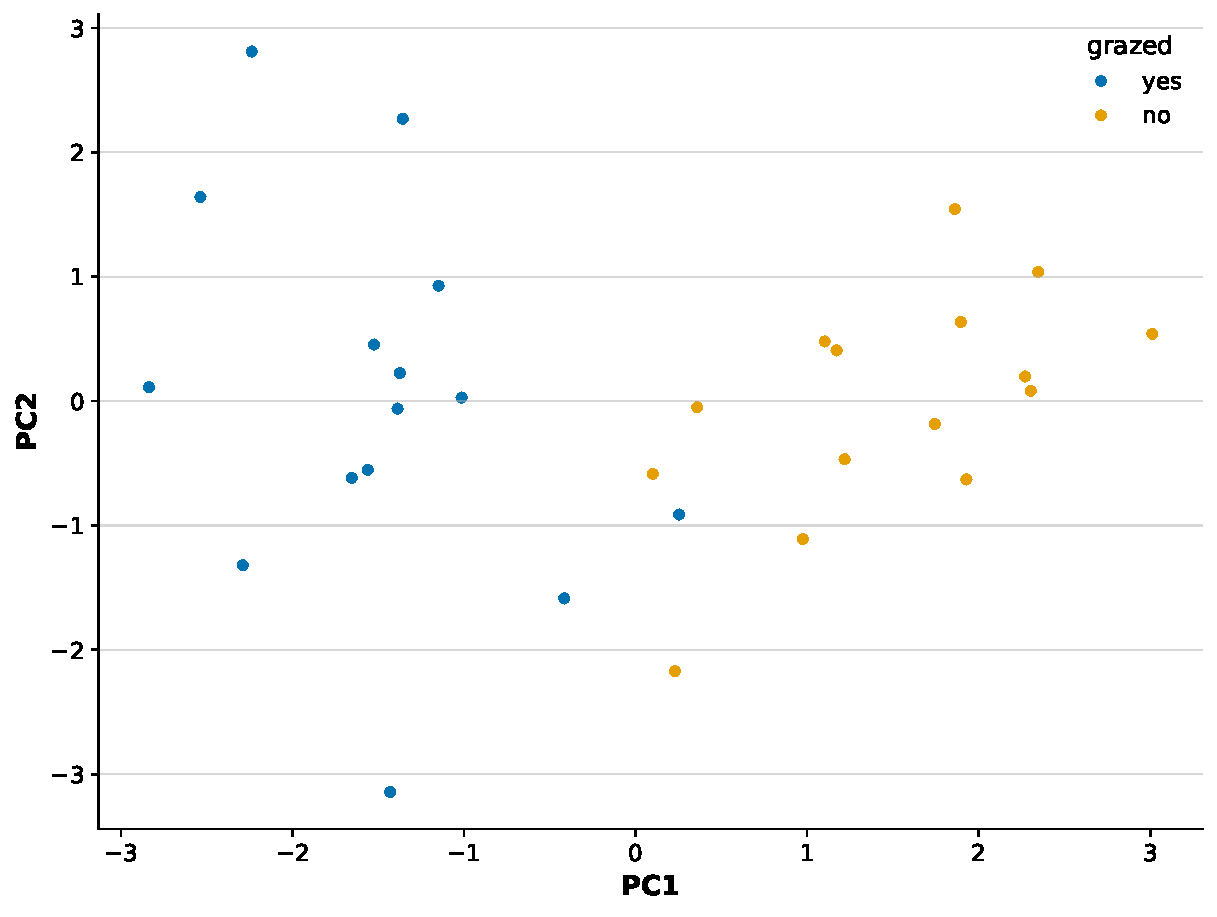
\includegraphics[width=0.72\textwidth,height=0.36\textheight,keepaspectratio]{figures/lesson17_example1_lesson17_pca.pdf}
\captionof{figure}{Lesson 17, example 1: \code{lesson17\_\allowbreak{}pca.\allowbreak{}png}.}
\end{minipage}\end{center}
\section*{Example 2}
Ecologists compare plots by how different their make-up is. Bray-Curtis is the usual distance for counts, and NMDS draws a map that keeps the order of the distances.
\begin{lstlisting}[style=py]
import simplydata as sdata
table = sdata.table(sdata.example("meadow"))
distances = table.distances_between_rows(measure="bray-curtis", names="plot")
distances.show_first_rows(3)
table.add_nmds(measure="bray-curtis")
table.compare_profiles(for_each="grazed")
chart = table.chart()
chart.dots(x="NMDS1", y="NMDS2", colour="grazed")
chart.save("lesson17_nmds.png")
\end{lstlisting}
\whateachline
\begin{lineexplain}
  \item[1] Load simplydata.
  \item[2] The meadow table.
  \item[3] A table of the Bray-Curtis distance between every pair of plots: 0 means the same plants in the same numbers, 1 means nothing in common.
  \item[4] Look at the first rows.
  \item[5] Non-metric multidimensional scaling (NMDS): adds NMDS1 and NMDS2. The stress (0.195) says how well the map keeps the distances: usable.
  \item[6] Do grazed and ungrazed plots differ in make-up? PERMANOVA tests all ten plants at once: grazing explains 25 \% of the differences (p = 0.001).
  \item[7] Start a chart.
  \item[8] The NMDS map.
  \item[9] Save it.
\end{lineexplain}
\printedoutput{output/lesson17_example2.txt}
\begin{center}\begin{minipage}{\linewidth}\centering
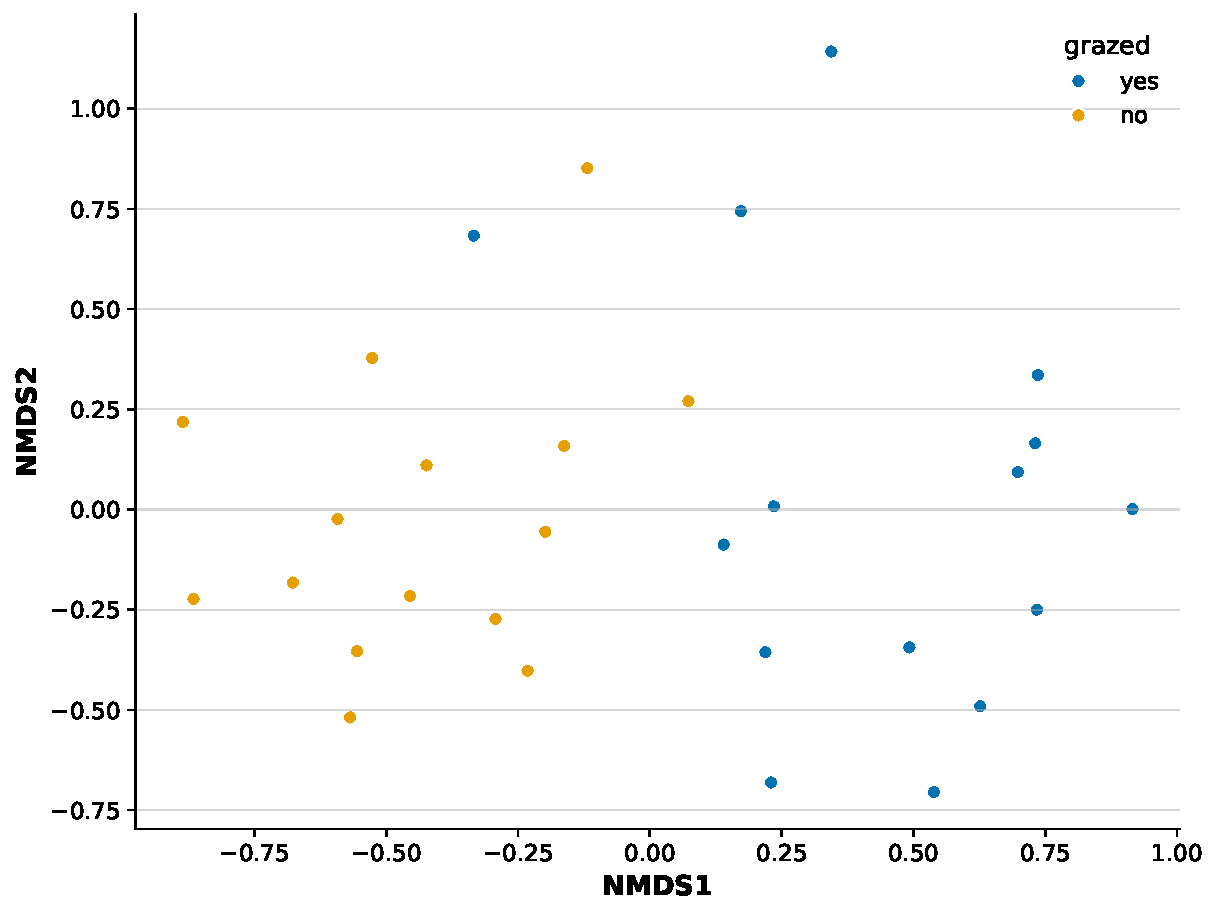
\includegraphics[width=0.72\textwidth,height=0.36\textheight,keepaspectratio]{figures/lesson17_example2_lesson17_nmds.pdf}
\captionof{figure}{Lesson 17, example 2: \code{lesson17\_\allowbreak{}nmds.\allowbreak{}png}.}
\end{minipage}\end{center}
\section*{Example 3}
Clustering finds groups of similar rows without being told the groups.
\begin{lstlisting}[style=py]
import simplydata as sdata
table = sdata.table(sdata.example("meadow"))
table.add_clusters(how_many=2)
table.count_rows(for_each="cluster", across="grazed")
\end{lstlisting}
\whateachline
\begin{lineexplain}
  \item[1] Load simplydata.
  \item[2] The meadow table.
  \item[3] k-means clustering: adds a column \code{\textquotedbl{}cluster\textquotedbl{}} with 1 or 2.
  \item[4] Did the clusters find the grazing? Cluster 1 is 14 grazed plots, cluster 2 is the 15 ungrazed plots and one grazed one.
\end{lineexplain}
\printedoutput{output/lesson17_example3.txt}
\begin{goodtoknow}
\begin{itemize}
  \item \code{same\_\allowbreak{}scale=True} (the normal choice for PCA and clusters) puts every column on the same scale first, so a column with big numbers does not drown the others.
  \item The signs and the rotation of PC and NMDS axes are arbitrary; only the distances between the dots mean something.
  \item Clarke's rule for NMDS stress: below 0.05 excellent, below 0.1 good, below 0.2 usable, above 0.2 hard to trust. Try \code{dimensions=3} if the stress is high.
  \item PERMANOVA can mistake a difference in spread for a difference in make-up, so \code{compare\_\allowbreak{}profiles} also checks the spread of each group and says if it differs.
  \item Clusters always appear, even in data without groups: check them against what you know.
  \item \code{method=\textquotedbl{}hierarchical\textquotedbl{}} clusters step by step (Ward linkage) instead of k-means.
\end{itemize}
\end{goodtoknow}
\begin{tryit}
\begin{enumerate}
  \item Add principal components of \code{\textquotedbl{}hours\textquotedbl{}}, \code{\textquotedbl{}sleep\textquotedbl{}}, \code{\textquotedbl{}marks\textquotedbl{}} and \code{\textquotedbl{}days\_\allowbreak{}absent\textquotedbl{}} in \code{sdata.\allowbreak{}example(\textquotedbl{}school\textquotedbl{})}. Which columns weigh most in PC1?
  \item Make an NMDS map of the meadow in 3 dimensions. Is the stress lower than in 2?
  \item Do the three fields differ in make-up? Use \code{compare\_\allowbreak{}profiles} with \code{for\_\allowbreak{}each=\textquotedbl{}field\textquotedbl{}}.
  \item Cluster the meadow plots with \code{method=\textquotedbl{}hierarchical\textquotedbl{}}. Do the clusters match the grazing?
\end{enumerate}
Worked solutions: page~\pageref{solutions:17}, or type \code{sdata.\allowbreak{}lesson(17,\allowbreak{} solutions=True)}.
\end{tryit}
\par\noindent{\small\sffamily\textbf{Words in this lesson:} \hyperref[word:table.add-principal-components]{\code{table.\allowbreak{}add\_\allowbreak{}principal\_\allowbreak{}components()}}, \hyperref[word:table.principal-components-of]{\code{table.\allowbreak{}principal\_\allowbreak{}components\_\allowbreak{}of()}}, \hyperref[word:table.add-clusters]{\code{table.\allowbreak{}add\_\allowbreak{}clusters()}}, \hyperref[word:table.distances-between-rows]{\code{table.\allowbreak{}distances\_\allowbreak{}between\_\allowbreak{}rows()}}, \hyperref[word:table.add-nmds]{\code{table.\allowbreak{}add\_\allowbreak{}nmds()}}, \hyperref[word:table.compare-profiles]{\code{table.\allowbreak{}compare\_\allowbreak{}profiles()}}, \hyperref[word:dots]{\code{chart.\allowbreak{}dots()}}.\par}

\chapter{Survival, and planning a study}\label{lesson:18}
\begin{learnbox}
\begin{itemize}
  \item how to draw survival curves (Kaplan-Meier) and compare them (log-rank test)
  \item how to explain the risk of an event from several columns (a Cox model)
  \item how many values a study needs, before you collect them (power analysis)
\end{itemize}
\end{learnbox}
\section*{Example 1}
In a trial, some patients are still alive when the follow-up ends. Survival words use their time too: they count as followed without the event (censored).
\begin{lstlisting}[style=py]
import simplydata as sdata
table = sdata.table(sdata.example("trial"))
table.survival_over_time(time="days", event="died", for_each="treatment")
chart = table.chart()
chart.survival_curves(time="days", event="died", colour="treatment", confidence_band=True, at_risk_table=True)
chart.save("lesson18_survival.png")
\end{lstlisting}
\whateachline
\begin{lineexplain}
  \item[1] Load simplydata.
  \item[2] 120 patients, a new medicine or usual care, followed for up to 3 years.
  \item[3] The Kaplan-Meier estimate: the share still alive at each time, and the median time (706 days with the new medicine, 545 with usual care).
  \item[4] Start a chart.
  \item[5] Survival curves with their 95 \% bands, ticks where patients were censored, and the number still followed under the x-axis.
  \item[6] Save it.
\end{lineexplain}
\printedoutput{output/lesson18_example1.txt}
\begin{center}\begin{minipage}{\linewidth}\centering
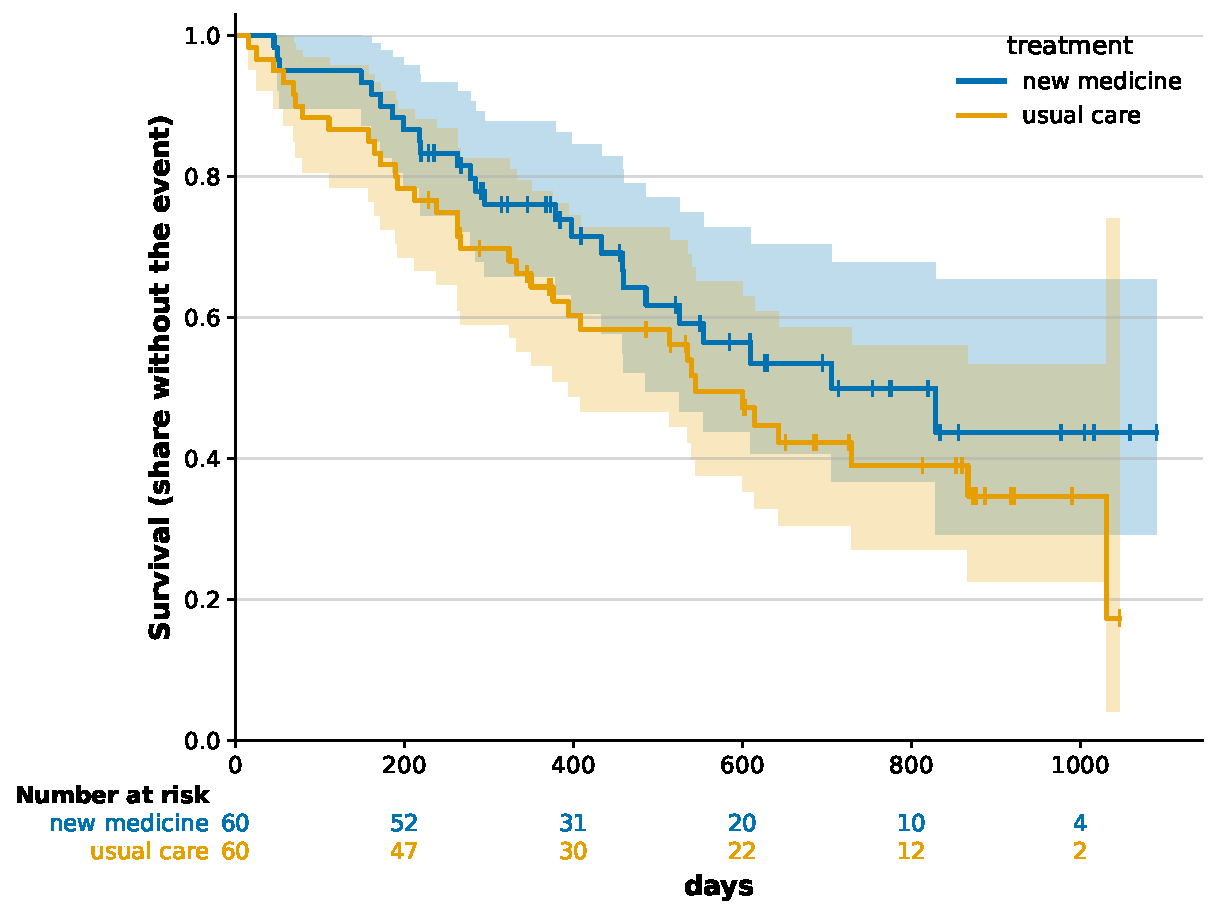
\includegraphics[width=0.72\textwidth,height=0.36\textheight,keepaspectratio]{figures/lesson18_example1_lesson18_survival.pdf}
\captionof{figure}{Lesson 18, example 1: \code{lesson18\_\allowbreak{}survival.\allowbreak{}png}.}
\end{minipage}\end{center}
\section*{Example 2}
Is the difference real? And what else changes the risk?
\begin{lstlisting}[style=py]
import simplydata as sdata
table = sdata.table(sdata.example("trial"))
table.compare_survival(time="days", event="died", for_each="treatment")
table.explain_survival(time="days", event="died", using=["treatment", "age"])
\end{lstlisting}
\whateachline
\begin{lineexplain}
  \item[1] Load simplydata.
  \item[2] The trial table.
  \item[3] The log-rank test compares the whole curves: here the difference could easily be chance (p = 0.22).
  \item[4] A Cox model: each year of age raises the risk of dying at any moment by about 5 \% (hazard ratio 1.05), with the treatment held fixed.
\end{lineexplain}
\printedoutput{output/lesson18_example2.txt}
\section*{Example 3}
Was the trial big enough? Power analysis tells you how many values you need before you collect them.
\begin{lstlisting}[style=py]
import simplydata as sdata
sdata.how_many_needed(effect_size=0.5, power=0.8)
sdata.chance_to_find(effect_size=0.5, values_per_group=20)
\end{lstlisting}
\whateachline
\begin{lineexplain}
  \item[1] Load simplydata.
  \item[2] To find a medium difference between two averages (half a standard deviation) with an 80 \% chance, you need 64 values in each group.
  \item[3] With only 20 values in each group, the chance to find it is just 34 \%.
\end{lineexplain}
\printedoutput{output/lesson18_example3.txt}
\begin{goodtoknow}
\begin{itemize}
  \item Never leave out the censored rows or count them as survivors: the survival words use the time they were followed, which is what makes these methods right.
  \item A hazard ratio above 1 means a higher risk of the event at any moment; 1 means no difference. The Cox model assumes the ratio stays the same over time, and simplydata checks this and says so if it does not.
  \item A study that is too small often finds nothing even when there is something to find. Plan the size before collecting data, not after.
  \item \code{effect\_\allowbreak{}size=} is Cohen's d for averages, f for 3 or more groups, w for counts and r for a correlation. You can also give \code{difference=} and \code{spread=} in your own units.
\end{itemize}
\end{goodtoknow}
\begin{tryit}
\begin{enumerate}
  \item Explain the risk of dying from \code{\textquotedbl{}age\textquotedbl{}} alone with \code{explain\_\allowbreak{}survival}.
  \item How many pairs does a before/after study need to find a small change (\code{effect\_\allowbreak{}size=0.\allowbreak{}3})?
  \item What is the chance to find a medium difference (\code{effect\_\allowbreak{}size=0.\allowbreak{}25}) between 3 groups with 30 values in each?
\end{enumerate}
Worked solutions: page~\pageref{solutions:18}, or type \code{sdata.\allowbreak{}lesson(18,\allowbreak{} solutions=True)}.
\end{tryit}
\par\noindent{\small\sffamily\textbf{Words in this lesson:} \hyperref[word:table.survival-over-time]{\code{table.\allowbreak{}survival\_\allowbreak{}over\_\allowbreak{}time()}}, \hyperref[word:survival-curves]{\code{chart.\allowbreak{}survival\_\allowbreak{}curves()}}, \hyperref[word:table.compare-survival]{\code{table.\allowbreak{}compare\_\allowbreak{}survival()}}, \hyperref[word:table.explain-survival]{\code{table.\allowbreak{}explain\_\allowbreak{}survival()}}, \hyperref[word:sdata.how-many-needed]{\code{sdata.\allowbreak{}how\_\allowbreak{}many\_\allowbreak{}needed()}}, \hyperref[word:sdata.chance-to-find]{\code{sdata.\allowbreak{}chance\_\allowbreak{}to\_\allowbreak{}find()}}.\par}

\chapter{Fitting curves, finding the best value and solving}\label{lesson:19}
\begin{learnbox}
\begin{itemize}
  \item how to fit a straight line, a curve or any formula to your data, on a table and on a chart
  \item how to find where a formula is smallest or biggest
  \item how to solve an equation, also one made from a fitted formula
\end{itemize}
\end{learnbox}
\section*{Example 1}
Start with something you know: a straight line through the dots. \code{fit\_\allowbreak{}line}, \code{fit\_\allowbreak{}curve} and \code{fit\_\allowbreak{}formula} are the same words on a table (the numbers) and on a chart (the picture).
\begin{lstlisting}[style=py]
import simplydata as sdata
table = sdata.table(sdata.example("marks"))
table.fit_line(x="hours", y="marks")
table.fit_curve(x="hours", y="marks", degree=2)
chart = table.chart()
chart.dots(x="hours", y="marks")
chart.fit_line()
chart.fit_curve(degree=2)
chart.save("lesson19_line_and_curve.png")
\end{lstlisting}
\whateachline
\begin{lineexplain}
  \item[1] Load simplydata.
  \item[2] The marks table: hours of study and marks.
  \item[3] The straight line: about 5.2 marks more for each hour of study, and R squared 0.69.
  \item[4] A curve with one bend (hours and hours**2). R squared only goes from 0.69 to 0.70, so the bend adds little: the straight line is enough here.
  \item[5] Start a chart of the same table.
  \item[6] The dots.
  \item[7] The same straight line, drawn.
  \item[8] And the curve, to see how close they are.
  \item[9] Save it.
\end{lineexplain}
\printedoutput{output/lesson19_example1.txt}
\begin{center}\begin{minipage}{\linewidth}\centering
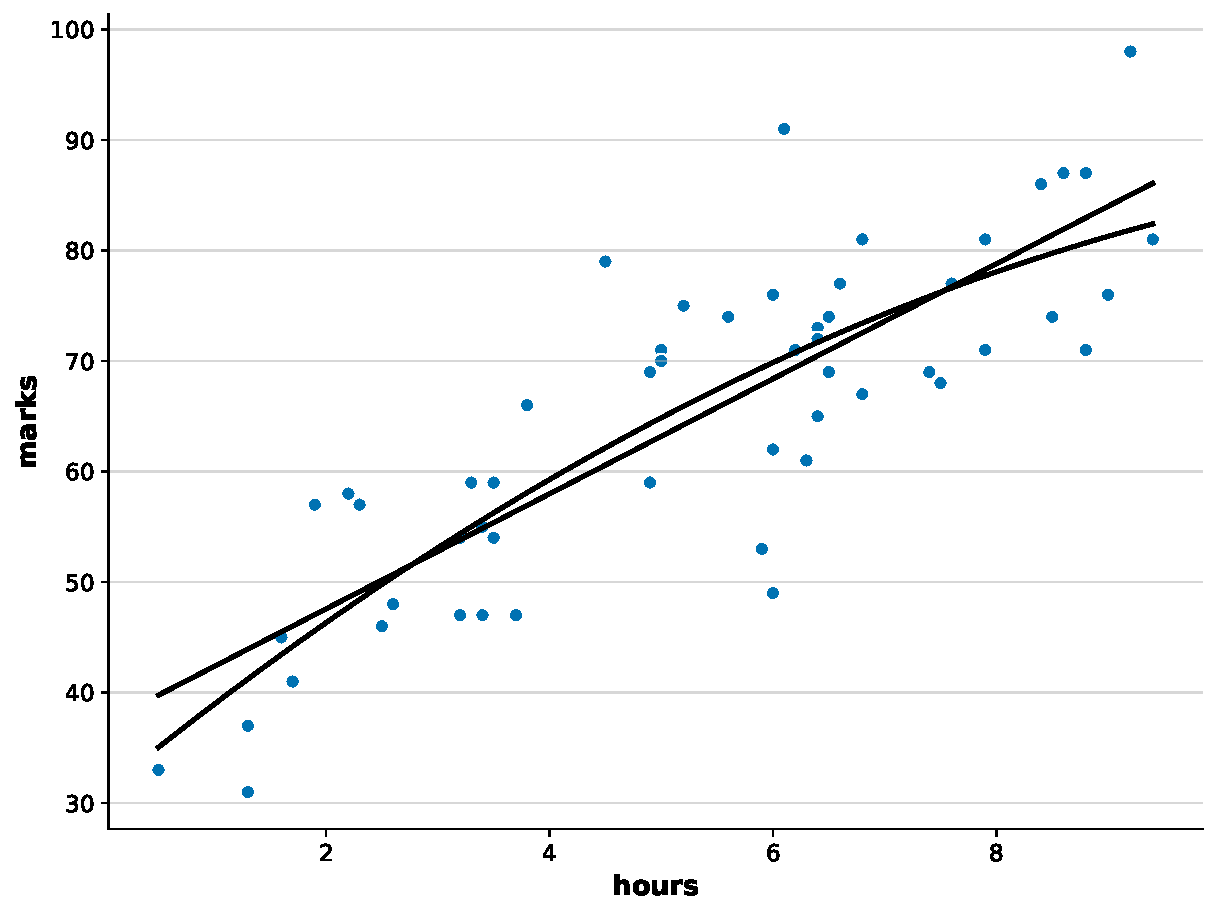
\includegraphics[width=0.72\textwidth,height=0.36\textheight,keepaspectratio]{figures/lesson19_example1_lesson19_line_and_curve.pdf}
\captionof{figure}{Lesson 19, example 1: \code{lesson19\_\allowbreak{}line\_\allowbreak{}and\_\allowbreak{}curve.\allowbreak{}png}.}
\end{minipage}\end{center}
\section*{Example 2}
A research question: how fast does each country grow? Growth by a fixed share each year is the formula population = a * \code{exp(b * (year - 2000))}. Names that are columns (population, year) are data; the other names (a, b) are the values to find.
\begin{lstlisting}[style=py]
import simplydata as sdata
table = sdata.table(sdata.example("growth"))
table.fit_formula("population = a * exp(b * (year - 2000))", for_each="country")
chart = table.chart()
chart.dots(x="year", y="population", colour="country")
chart.fit_formula("population = a * exp(b * (year - 2000))")
chart.save("lesson19_growth.png")
\end{lstlisting}
\whateachline
\begin{lineexplain}
  \item[1] Load simplydata.
  \item[2] Four countries, every two years.
  \item[3] One fit for each country, by nonlinear least squares (as R \code{nls()}). a is the population in 2000 and b the growth rate: Cherria grows fastest, b = 0.0443, about 4.5 \% a year.
  \item[4] Start a chart.
  \item[5] The data, one colour per country.
  \item[6] The fitted curve of each country, with the same values as the table word.
  \item[7] Save it.
\end{lineexplain}
\printedoutput{output/lesson19_example2.txt}
\begin{center}\begin{minipage}{\linewidth}\centering
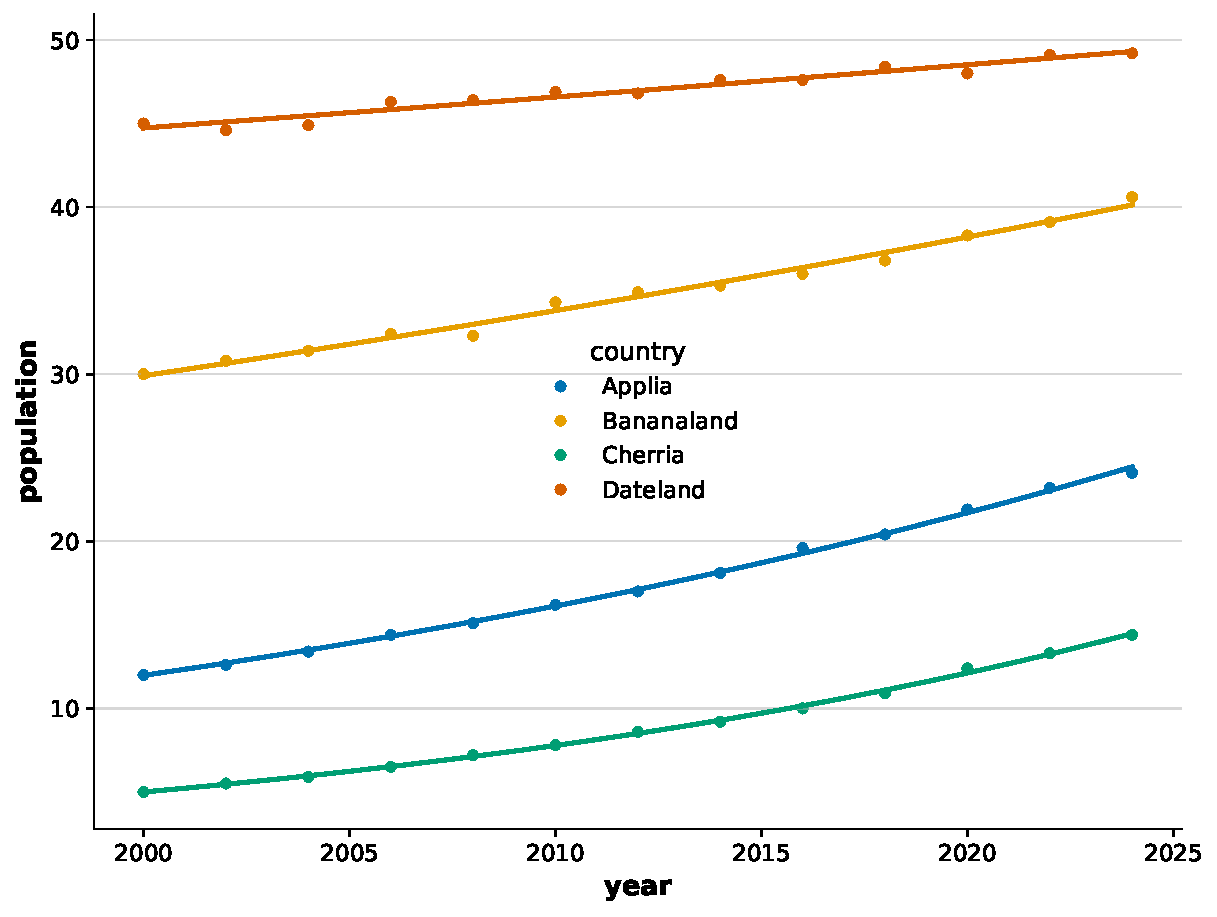
\includegraphics[width=0.72\textwidth,height=0.36\textheight,keepaspectratio]{figures/lesson19_example2_lesson19_growth.pdf}
\captionof{figure}{Lesson 19, example 2: \code{lesson19\_\allowbreak{}growth.\allowbreak{}png}.}
\end{minipage}\end{center}
\section*{Example 3}
Finding and solving: \code{sdata.\allowbreak{}find\_\allowbreak{}smallest}, \code{sdata.\allowbreak{}find\_\allowbreak{}biggest} and \code{sdata.\allowbreak{}solve} work on a formula. The names in it are what to find; \code{between=} says where to look.
\begin{lstlisting}[style=py]
import simplydata as sdata
sdata.find_smallest("x**2 - 4*x + 1", between=[0, 5])
sdata.find_biggest("3*x + 2*y", rules=["x + y <= 4", "x + 3*y <= 6", "x >= 0", "y >= 0"])
sdata.solve("x**3 - 2*x = 5", between=[0, 3])
table = sdata.table(sdata.example("growth"))
table.keep_rows("country", equal_to="Applia")
fit = table.fit_formula("population = a * exp(b * (year - 2000))")
sdata.solve("a * exp(b * (year - 2000)) = 20", between=[2000, 2050], known=fit)
\end{lstlisting}
\whateachline
\begin{lineexplain}
  \item[1] Load simplydata.
  \item[2] The smallest value is -3, at x = 2. The method and its R name are printed (R \code{optimize()}).
  \item[3] The biggest value under rules: 12, at x = 4 and y = 0. Everything is a straight line, so simplydata uses linear programming and says which rules are reached exactly.
  \item[4] The value of x that makes both sides equal: 2.09455. Every solution in the range is found.
  \item[5] Back to the growth table.
  \item[6] Keep one country.
  \item[7] Fit the growth formula and keep the result, a one-row table with a and b.
  \item[8] \code{known=fit} puts the fitted a and b into the equation: Applia reaches 20 million in about 2017 (year = 2017.24). A fitted curve answers questions, not only draws a line.
\end{lineexplain}
\printedoutput{output/lesson19_example3.txt}
\begin{goodtoknow}
\begin{itemize}
  \item Fitting is the same idea every time: a line, a curve or a formula is moved until it is as close to the points as it can be (least squares). The printed sentence says how sure each value is (its 95 \% confidence interval).
  \item A curve with a high \code{degree=} can wiggle through every point and still say nothing true. Choose the simplest line or formula that follows the data, and a formula whose values mean something (here b is a growth rate).
  \item If a formula fit fails, give start values near the answer: \code{start=}\{\code{\textquotedbl{}a\textquotedbl{}}: 10, \code{\textquotedbl{}b\textquotedbl{}}: 0.03\}.
  \item \code{find\_\allowbreak{}smallest} with \code{between=} finds one lowest point; when the curve has several dips it says so, and \code{search=\textquotedbl{}whole range\textquotedbl{}} looks everywhere. solve with \code{between=} finds every crossing.
  \item Names from other tools point to these words: minimize, optimise and argmin to \code{find\_\allowbreak{}smallest}, fsolve, brentq and uniroot to solve, \code{curve\_\allowbreak{}fit} and nls to \code{fit\_\allowbreak{}formula}, polyfit to \code{fit\_\allowbreak{}curve}.
\end{itemize}
\end{goodtoknow}
\begin{tryit}
\begin{enumerate}
  \item Fit a curve of degree 3 to \code{\textquotedbl{}marks\textquotedbl{}} against \code{\textquotedbl{}hours\textquotedbl{}}. Does R squared go up much from the straight line?
  \item With the weather table, keep the city Sunnyvale and fit \code{\textquotedbl{}temperature = a + b * cos(2 * pi * (month\_\allowbreak{}number - c) / 12)\textquotedbl{}} with \code{start=}\{\code{\textquotedbl{}a\textquotedbl{}}: 15, \code{\textquotedbl{}b\textquotedbl{}}: 8, \code{\textquotedbl{}c\textquotedbl{}}: 7\}. In which month is it warmest (c)?
  \item Try to remember without looking back: which word finds where a formula is biggest, and which word finds where the two sides of an equation are equal? Use them on \code{\textquotedbl{}x * (10 - x)\textquotedbl{}} between 0 and 10, and on \code{\textquotedbl{}x**2 = 2\textquotedbl{}} between 0 and 2.
\end{enumerate}
Worked solutions: page~\pageref{solutions:19}, or type \code{sdata.\allowbreak{}lesson(19,\allowbreak{} solutions=True)}.
\end{tryit}
\par\noindent{\small\sffamily\textbf{Words in this lesson:} \hyperref[word:table.fit-line]{\code{table.\allowbreak{}fit\_\allowbreak{}line()}}, \hyperref[word:table.fit-curve]{\code{table.\allowbreak{}fit\_\allowbreak{}curve()}}, \hyperref[word:table.fit-formula]{\code{table.\allowbreak{}fit\_\allowbreak{}formula()}}, \hyperref[word:fit-line]{\code{chart.\allowbreak{}fit\_\allowbreak{}line()}}, \hyperref[word:fit-curve]{\code{chart.\allowbreak{}fit\_\allowbreak{}curve()}}, \hyperref[word:fit-formula]{\code{chart.\allowbreak{}fit\_\allowbreak{}formula()}}, \hyperref[word:sdata.find-smallest]{\code{sdata.\allowbreak{}find\_\allowbreak{}smallest()}}, \hyperref[word:sdata.find-biggest]{\code{sdata.\allowbreak{}find\_\allowbreak{}biggest()}}, \hyperref[word:sdata.solve]{\code{sdata.\allowbreak{}solve()}}.\par}

\chapter{Distributions, chances and values between points}\label{lesson:20}
\begin{learnbox}
\begin{itemize}
  \item how to ask a distribution for chances, percentiles and cut-offs
  \item how to find which distribution fits your data, and check it
  \item how to estimate values between the points you measured
\end{itemize}
\end{learnbox}
\section*{Example 1}
A distribution says how likely each value is. Start with the bell curve (normal): marks with an average of 50 and a standard deviation of 10.
\begin{lstlisting}[style=py]
import simplydata as sdata
dist = sdata.distribution("normal", average=50, standard_deviation=10)
dist.chance(above=80)
dist.chance(between=[40, 60])
dist.percentile(95)
dist.cut_off(above=0.025)
chart = dist.chart()
chart.save("lesson20_normal.png")
\end{lstlisting}
\whateachline
\begin{lineexplain}
  \item[1] Load simplydata.
  \item[2] Make the distribution. R's names (\code{mean=}, \code{sd=}) work too.
  \item[3] The chance of a mark above 80: 0.135 \%. The R code that gives the same answer is printed too: \code{pnorm(80,\allowbreak{} .\allowbreak{}.\allowbreak{}.\allowbreak{})}.
  \item[4] 68.3 \%: about two in three are within one standard deviation of the average.
  \item[5] 95 \% of marks are below 66.4.
  \item[6] The cut-off with a 2.5 \% chance above it: 69.6. Tests use such cut-offs (critical values).
  \item[7] A chart of the bell curve.
  \item[8] Save it.
\end{lineexplain}
\printedoutput{output/lesson20_example1.txt}
\begin{center}\begin{minipage}{\linewidth}\centering
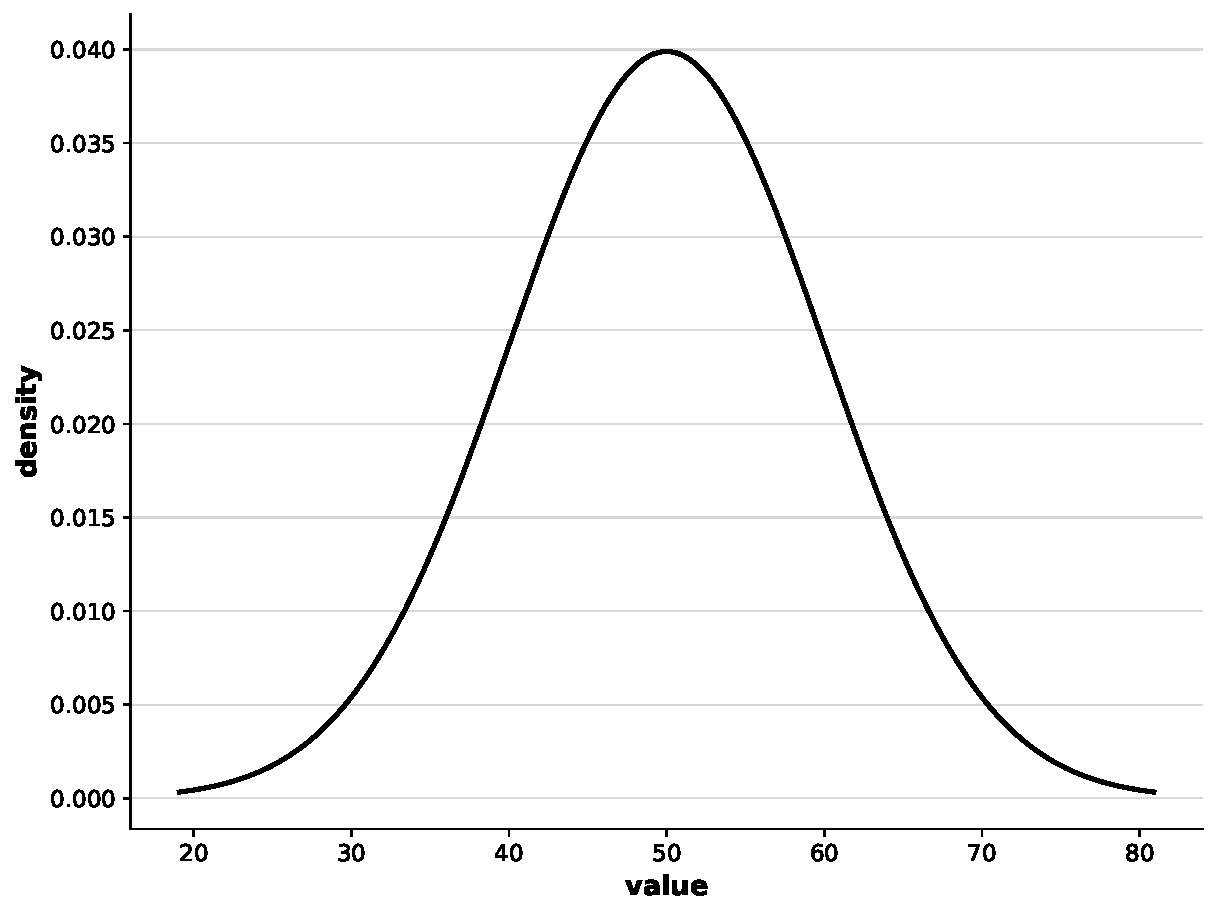
\includegraphics[width=0.72\textwidth,height=0.36\textheight,keepaspectratio]{figures/lesson20_example1_lesson20_normal.pdf}
\captionof{figure}{Lesson 20, example 1: \code{lesson20\_\allowbreak{}normal.\allowbreak{}png}.}
\end{minipage}\end{center}
\section*{Example 2}
A research question: pupils' days absent are counts (0, 1, 2 ...). Do they vary as a Poisson distribution expects, or more? The words that fit are \code{fit\_\allowbreak{}distribution} and \code{compare\_\allowbreak{}distributions}.
\begin{lstlisting}[style=py]
import simplydata as sdata
table = sdata.table(sdata.example("school"))
table.compare_distributions("days_absent", distributions=("poisson", "negative binomial"))
fit = table.fit_distribution("days_absent", "negative binomial")
fit.chance(at_least=10)
chart = table.chart()
chart.histogram(x="days_absent", show="density")
chart.fit_distribution("negative binomial")
chart.save("lesson20_absent.png")
\end{lstlisting}
\whateachline
\begin{lineexplain}
  \item[1] Load simplydata.
  \item[2] 180 pupils and their days absent.
  \item[3] Both are fitted by maximum likelihood and ranked by AIC: the negative binomial wins by 7, so the counts vary more than Poisson allows.
  \item[4] Fit it and keep the fitted distribution.
  \item[5] The chance a pupil misses 10 days or more: 0.66 \%.
  \item[6] Start a chart.
  \item[7] The counts, as shares.
  \item[8] The fitted chance of each count, on top.
  \item[9] Save it.
\end{lineexplain}
\printedoutput{output/lesson20_example2.txt}
\begin{center}\begin{minipage}{\linewidth}\centering
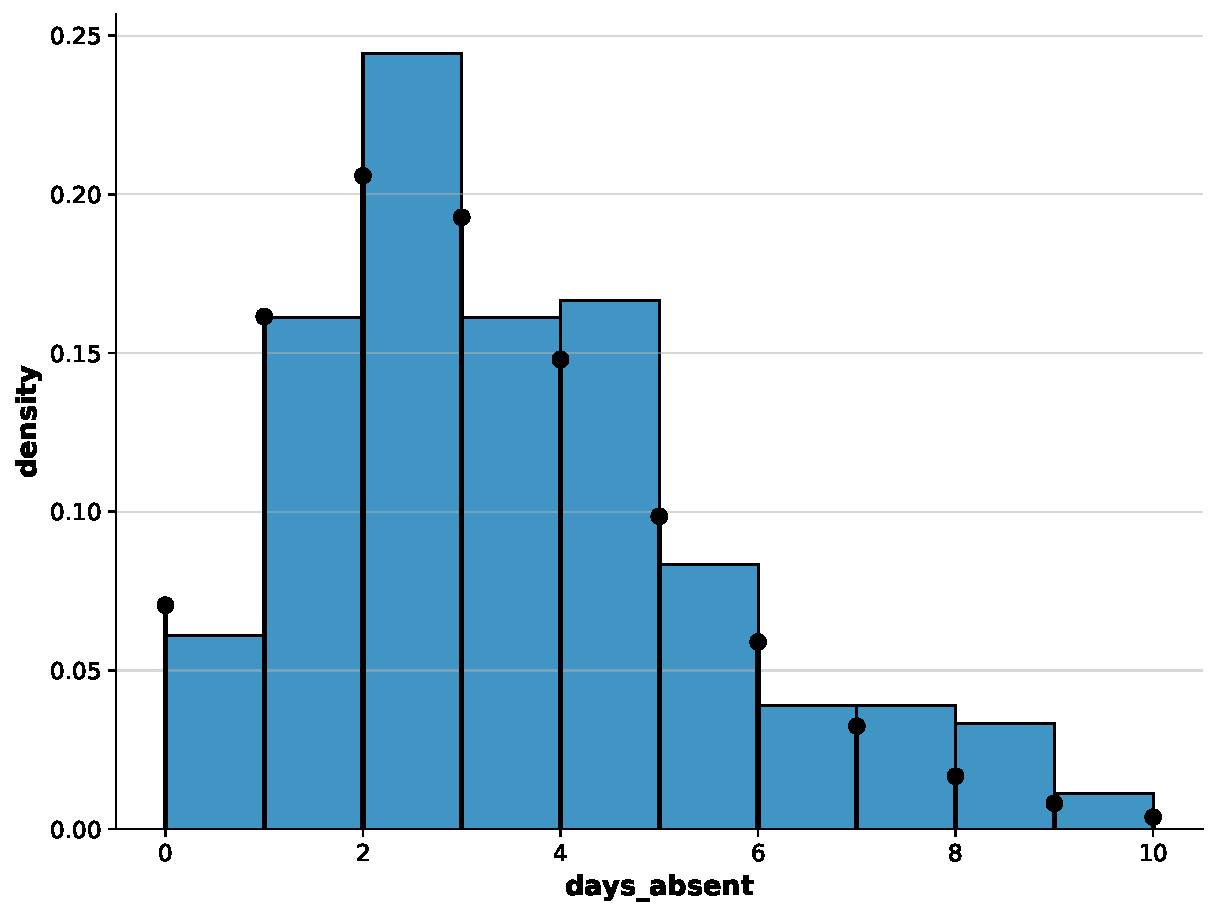
\includegraphics[width=0.72\textwidth,height=0.36\textheight,keepaspectratio]{figures/lesson20_example2_lesson20_absent.pdf}
\captionof{figure}{Lesson 20, example 2: \code{lesson20\_\allowbreak{}absent.\allowbreak{}png}.}
\end{minipage}\end{center}
\section*{Example 3}
Values between points: you measured every two years, but you need 2001. \code{values\_\allowbreak{}at} joins the dots (straight lines, or a smooth curve) and reads off the value; \code{map\_\allowbreak{}of} does it across a whole map.
\begin{lstlisting}[style=py]
import simplydata as sdata
table = sdata.table(sdata.example("growth"))
estimates = table.values_at("population", at={"year": [2001, 2011]}, for_each="country")
estimates.show()
island = sdata.table(sdata.example("island"))
heights = island.map_of("height", across=["east", "north"], steps=60, joined_by="smooth surface")
chart = heights.chart()
chart.contour(x="east", y="north", z="height")
chart.save("lesson20_map.png")
\end{lstlisting}
\whateachline
\begin{lineexplain}
  \item[1] Load simplydata.
  \item[2] Population every two years.
  \item[3] Straight lines between the known points (linear interpolation, as R \code{approx()}), for each country.
  \item[4] A new table with the estimates.
  \item[5] Heights measured on a 15 x 15 grid.
  \item[6] A finer 60 x 60 map, with a smooth surface through every point (a thin-plate spline).
  \item[7] A chart of the new map.
  \item[8] Its contour map.
  \item[9] Save it.
\end{lineexplain}
\printedoutput{output/lesson20_example3.txt}
\begin{center}\begin{minipage}{\linewidth}\centering
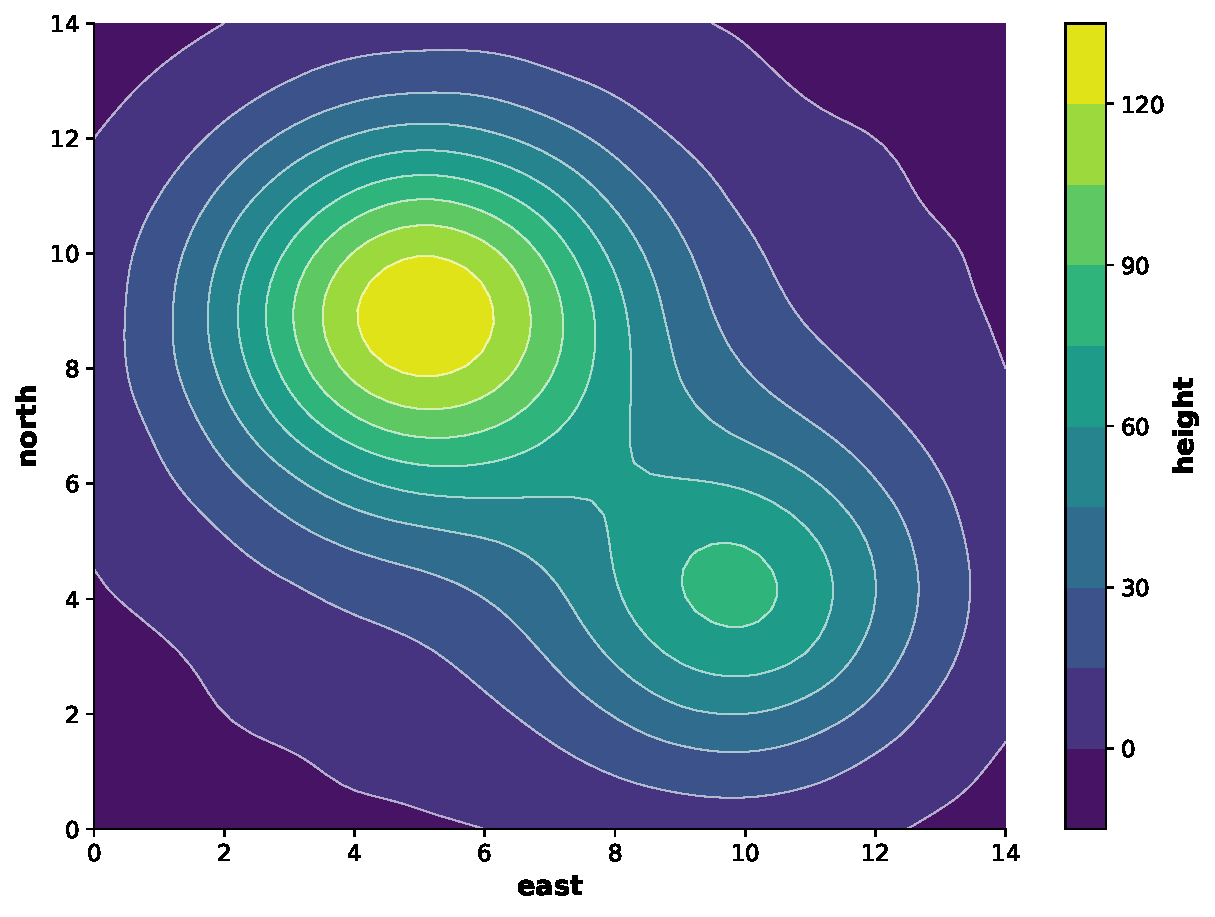
\includegraphics[width=0.72\textwidth,height=0.36\textheight,keepaspectratio]{figures/lesson20_example3_lesson20_map.pdf}
\captionof{figure}{Lesson 20, example 3: \code{lesson20\_\allowbreak{}map.\allowbreak{}png}.}
\end{minipage}\end{center}
\begin{goodtoknow}
\begin{itemize}
  \item \code{chance()} gives back a share from 0 to 1 and prints it as a percent. \code{above=} and \code{below=} leave the value itself out, \code{at\_\allowbreak{}least=} and \code{at\_\allowbreak{}most=} keep it in, as in \code{keep\_\allowbreak{}rows}. For counts that matters: \code{at\_\allowbreak{}most=3} means 3 or fewer.
  \item \code{density\_\allowbreak{}at()} is the height of the curve, not a chance: a chance is an area under the curve, so ask \code{chance(between=[.\allowbreak{}.\allowbreak{}.\allowbreak{}])}.
  \item A fitted distribution is only as good as its fit. Compare a few with \code{compare\_\allowbreak{}distributions}, and test the shape with \code{table.\allowbreak{}compare\_\allowbreak{}shape\_\allowbreak{}to(\textquotedbl{}column\textquotedbl{},\allowbreak{} \textquotedbl{}gamma\textquotedbl{})}.
  \item Values between points are estimates. Straight lines are the safe choice; a smooth curve can swing above or below the points (\code{joined\_\allowbreak{}by=\textquotedbl{}curve without overshoot\textquotedbl{}} never does). Outside the measured range the cells stay empty unless you ask for \code{outside=}.
  \item Names from other tools point to these words: pnorm and cdf to chance, qnorm and ppf to percentile, dnorm and pdf to \code{density\_\allowbreak{}at}, interpolate and approx to \code{values\_\allowbreak{}at}.
\end{itemize}
\end{goodtoknow}
\begin{tryit}
\begin{enumerate}
  \item Ten coins are thrown. With \code{sdata.\allowbreak{}distribution(\textquotedbl{}binomial\textquotedbl{},\allowbreak{} tries=10,\allowbreak{} chance=0.\allowbreak{}5)}, what is the chance of 8 heads or more?
  \item Which fits the daily \code{\textquotedbl{}sales\textquotedbl{}} of the shop table best: normal, lognormal, gamma or weibull? Then check the best one with \code{compare\_\allowbreak{}shape\_\allowbreak{}to}.
  \item Try to remember without looking back: which word estimates a value between the points you measured? Use it to estimate the temperature of each city at \code{month\_\allowbreak{}number} 6.5, joined by a smooth curve.
\end{enumerate}
Worked solutions: page~\pageref{solutions:20}, or type \code{sdata.\allowbreak{}lesson(20,\allowbreak{} solutions=True)}.
\end{tryit}
\par\noindent{\small\sffamily\textbf{Words in this lesson:} \hyperref[word:sdata.distribution]{\code{sdata.\allowbreak{}distribution()}}, \hyperref[word:dist.chance]{\code{dist.\allowbreak{}chance()}}, \hyperref[word:dist.percentile]{\code{dist.\allowbreak{}percentile()}}, \hyperref[word:dist.cut-off]{\code{dist.\allowbreak{}cut\_\allowbreak{}off()}}, \hyperref[word:dist.chart]{\code{dist.\allowbreak{}chart()}}, \hyperref[word:table.compare-distributions]{\code{table.\allowbreak{}compare\_\allowbreak{}distributions()}}, \hyperref[word:table.fit-distribution]{\code{table.\allowbreak{}fit\_\allowbreak{}distribution()}}, \hyperref[word:fit-distribution]{\code{chart.\allowbreak{}fit\_\allowbreak{}distribution()}}, \hyperref[word:table.values-at]{\code{table.\allowbreak{}values\_\allowbreak{}at()}}, \hyperref[word:table.map-of]{\code{table.\allowbreak{}map\_\allowbreak{}of()}}, \hyperref[word:curve]{\code{chart.\allowbreak{}curve()}}.\par}

\otherchapters

\part{Dictionary of words}\label{part:dictionary}

\unchapter{How to read the dictionary}{dictionary:how}

Each entry gives the word as you type it, what it does (in the words of \code{sdata.\allowbreak{}help(\textquotedbl{}word\textquotedbl{})}), the options you can put in its brackets and what they normally are, the library that does the work underneath, and an example you can run as it is. The same entries are in Python: \code{sdata.\allowbreak{}help(\textquotedbl{}bars\textquotedbl{})}. The words come in the same groups as \code{sdata.\allowbreak{}words()}; the \hyperref[index]{index of words} at the end of the book lists them A to Z.

\unchapter{Chart words}{family:chart}
Steps on a chart: \code{chart = sdata.chart(table)}, then \code{chart.bars(...)}. Words that start with \code{sdata.} are called on simplydata itself, and words that end in \code{=} are options inside a chart step.
\unsection{Start, show and save}{group:Start-show-and-save}
\wordentry{sdata.chart()}{word:sdata.chart}
Start a chart. \code{sdata.\allowbreak{}chart(sdata.\allowbreak{}example(\textquotedbl{}marks\textquotedbl{}))}

\codeline{sdata.chart(table)}\enspace a pandas or Polars table, like \code{sdata.\allowbreak{}example(\textquotedbl{}marks\textquotedbl{})}\\
\codeline{sdata.chart(\textquotedbl{}my\_file.xlsx\textquotedbl{})}\enspace your own file (Excel, CSV, TSV, Parquet, JSON)\\
\codeline{sdata.chart(\textquotedbl{}my\_file.xlsx\textquotedbl{}, sheet=\textquotedbl{}2026\textquotedbl{}) one sheet of an Excel file}\\
\codeline{sdata.chart()}\enspace no table: give lists to each step instead\\
\codeline{fast=True}\enspace always use the fast engine (Polars) to read the file

\wordfield{Options}{}\par\nopagebreak
\begin{optiontable}
\code{data=} & \\
\code{sheet=} & \\
\code{fast=} & normally \code{False}\\
\end{optiontable}

\wordfield{Underneath}{pandas reads the file (Polars for big files); the chart is drawn with matplotlib and seaborn}
\wordfield{Example you can run}{(it uses the practice table \code{marks})}\par\nopagebreak
\begin{lstlisting}[style=py]
import simplydata as sdata
marks = sdata.example("marks")
chart = sdata.chart(marks)
chart.dots(x="hours", y="marks")
chart.save("my_chart.png")
\end{lstlisting}
\wordentry{sdata.example()}{word:sdata.example}
A small made-up table to practise with. \code{sdata.\allowbreak{}example(\textquotedbl{}marks\textquotedbl{})}

\codeline{sdata.example() with no name lists every table and its columns.}\\
The tables are: marks, weather, fruit, growth, shop, school, meadow, trial, island. \code{\textquotedbl{}shop\textquotedbl{}} has empty cells and a column of dates to practise with; \code{\textquotedbl{}school\textquotedbl{}} has empty cells too.

\wordfield{Options}{}\par\nopagebreak
\begin{optiontable}
\code{name=} & \\
\end{optiontable}

\wordfield{Underneath}{pandas (\code{read\_\allowbreak{}csv} of a small file inside simplydata)}
\wordfield{Example you can run}{(it uses the practice table \code{marks})}\par\nopagebreak
\begin{lstlisting}[style=py]
import simplydata as sdata
sdata.example()
marks = sdata.example("marks")
print(marks)
\end{lstlisting}
\wordentry{chart.show()}{word:show}
Show the chart in a window. \code{chart.\allowbreak{}show()}

In Jupyter, VS Code and Spyder charts appear by themselves.

\wordfield{Options}{none: just write the empty brackets.}

\wordfield{Good to know}{Not the same as the \code{show=} option inside bars and lines: for that, type \code{sdata.\allowbreak{}help(\textquotedbl{}show=\textquotedbl{})}.}

\wordfield{Underneath}{matplotlib (pyplot.show)}
\wordfield{Example you can run}{(it uses the practice table \code{marks})}\par\nopagebreak
\begin{lstlisting}[style=py]
import simplydata as sdata
marks = sdata.example("marks")
chart = sdata.chart(marks)
chart.bars(x="name", y="marks")
chart.show()
chart.save("marks.png")
\end{lstlisting}
\wordentry{chart.save()}{word:save}
Save the chart. \code{chart.\allowbreak{}save(\textquotedbl{}marks.\allowbreak{}png\textquotedbl{})} or \code{chart.\allowbreak{}save(\textquotedbl{}marks.\allowbreak{}tif\textquotedbl{},\allowbreak{} resolution=600)}

The end of the file name decides the format: \code{\textquotedbl{}marks.\allowbreak{}png\textquotedbl{}}, \code{\textquotedbl{}marks.\allowbreak{}pdf\textquotedbl{}}. \code{resolution=} is the sharpness in dots per inch (dpi); normally 300.

\wordfield{Options}{}\par\nopagebreak
\begin{optiontable}
\code{file\_\allowbreak{}name} & needed\\
\code{quality=} & normally \code{\textquotedbl{}normal\textquotedbl{}}\\
\code{resolution=} & \\
\code{dpi=} & \\
\end{optiontable}

\wordfield{Good to know}{File types: \code{.\allowbreak{}png} (a picture), \code{.\allowbreak{}pdf} and \code{.\allowbreak{}svg} (sharp at any size, good for printing), \code{.\allowbreak{}jpg}, \code{.\allowbreak{}tif}, and \code{.\allowbreak{}gif} for animations. \code{resolution=} is how sharp a picture is, in dots per inch (dpi): 300 is normal, journals often ask for 300 or 600 (\code{dpi=} means the same). \code{quality=\textquotedbl{}high\textquotedbl{}} is the same as \code{resolution=600}. \code{.\allowbreak{}tif} files are compressed without losing anything. To choose the size of the file in cm, mm or pixels, use \code{chart.\allowbreak{}size()} first.}

\wordfield{Underneath}{matplotlib (Figure.savefig); Pillow writes \code{.\allowbreak{}gif} animations}
\wordfield{Example you can run}{(it uses the practice table \code{marks})}\par\nopagebreak
\begin{lstlisting}[style=py]
import simplydata as sdata
marks = sdata.example("marks")
chart = sdata.chart(marks)
chart.bars(x="name", y="marks")
chart.save("marks.png")
chart.save("marks.pdf")
chart.save("marks.tif", resolution=600)
\end{lstlisting}
\unsection{Chart types}{group:Chart-types}
\wordentry{chart.bars()}{word:bars}
\wordfield{Also written}{\code{chart.\allowbreak{}bar()}}
Bars. \code{chart.\allowbreak{}bars(x=\textquotedbl{}name\textquotedbl{},\allowbreak{} y=\textquotedbl{}marks\textquotedbl{})} (with \code{sdata.\allowbreak{}example(\textquotedbl{}marks\textquotedbl{})})

\code{colour=\textquotedbl{}class\textquotedbl{}} gives each group its own colour, or \code{colour=\textquotedbl{}blue\textquotedbl{}} one colour. \code{show=} says what each bar stands for when a group has many rows: \code{\textquotedbl{}average\textquotedbl{}} (default), \code{\textquotedbl{}median\textquotedbl{}}, \code{\textquotedbl{}total\textquotedbl{}}, \code{\textquotedbl{}count\textquotedbl{}}, \code{\textquotedbl{}smallest\textquotedbl{}}, \code{\textquotedbl{}biggest\textquotedbl{}} or \code{\textquotedbl{}standard deviation\textquotedbl{}}. \code{error=\textquotedbl{}standard deviation\textquotedbl{}}, \code{\textquotedbl{}standard error\textquotedbl{}} or \code{\textquotedbl{}confidence interval\textquotedbl{}} adds error bars (with \code{show=\textquotedbl{}average\textquotedbl{}}); a line says which one was drawn. \code{stacked=True} puts groups on top of each other; \code{sideways=True} lays bars down. \code{transparency=0.\allowbreak{}5} makes them half see-through (0 is solid).

\wordfield{Options}{}\par\nopagebreak
\begin{optiontable}
\code{x=} & \\
\code{y=} & \\
\code{colour=} & \\
\code{show=} & normally \code{\textquotedbl{}average\textquotedbl{}}\\
\code{error=} & \\
\code{stacked=} & normally \code{False}\\
\code{sideways=} & normally \code{False}\\
\code{transparency=} & \\
\end{optiontable}

\wordfield{Underneath}{seaborn (barplot; countplot for \code{show=\textquotedbl{}count\textquotedbl{}})}
\wordfield{Example you can run}{(it uses the practice table \code{marks})}\par\nopagebreak
\begin{lstlisting}[style=py]
import simplydata as sdata
marks = sdata.example("marks")
chart = sdata.chart(marks)
chart.bars(x="name", y="marks", colour="class")
chart.rotate_labels_x()
chart.save("bars.png")
\end{lstlisting}
\wordentry{chart.lines()}{word:lines}
\wordfield{Also written}{\code{chart.\allowbreak{}line()}}
Lines. \code{chart.\allowbreak{}lines(x=\textquotedbl{}month\textquotedbl{},\allowbreak{} y=\textquotedbl{}temperature\textquotedbl{},\allowbreak{} colour=\textquotedbl{}city\textquotedbl{})} (with \code{sdata.\allowbreak{}example(\textquotedbl{}weather\textquotedbl{})})

\code{colour=\textquotedbl{}city\textquotedbl{}} draws one line per group. \code{dots=True} marks each point. \code{dashed=True} draws a dashed line. \code{show=} works as in bars (not \code{\textquotedbl{}count\textquotedbl{}}). \code{error=\textquotedbl{}standard deviation\textquotedbl{}}, \code{\textquotedbl{}standard error\textquotedbl{}} or \code{\textquotedbl{}confidence interval\textquotedbl{}} adds a shaded band; a line says which one was drawn. \code{thickness=3} draws thicker lines (normal is 2, in points); \code{transparency=0.\allowbreak{}5} makes them half see-through (0 is solid). \code{joined\_\allowbreak{}by=} says how the points are joined, as in \code{table.\allowbreak{}values\_\allowbreak{}at()}: \code{\textquotedbl{}straight lines\textquotedbl{}} (normal), \code{\textquotedbl{}smooth curve\textquotedbl{}} (natural cubic spline), \code{\textquotedbl{}curve without overshoot\textquotedbl{}} (PCHIP), \code{\textquotedbl{}steps\textquotedbl{}} (each value stays until the next point), \code{\textquotedbl{}nearest\textquotedbl{}}; experts: \code{\textquotedbl{}akima\textquotedbl{}}, \code{\textquotedbl{}makima\textquotedbl{}}, \code{\textquotedbl{}not-a-knot\textquotedbl{}}, \code{\textquotedbl{}periodic\textquotedbl{}}. Curves need numbers on x and y.

\wordfield{Options}{}\par\nopagebreak
\begin{optiontable}
\code{x=} & \\
\code{y=} & \\
\code{colour=} & \\
\code{show=} & normally \code{\textquotedbl{}average\textquotedbl{}}\\
\code{error=} & \\
\code{dots=} & normally \code{False}\\
\code{dashed=} & normally \code{False}\\
\code{thickness=} & \\
\code{transparency=} & \\
\code{joined\_\allowbreak{}by=} & normally \code{\textquotedbl{}straight lines\textquotedbl{}}\\
\end{optiontable}

\wordfield{Underneath}{seaborn (lineplot); SciPy (interpolate) for \code{joined\_\allowbreak{}by=} curves}
\wordfield{Example you can run}{(it uses the practice table \code{weather})}\par\nopagebreak
\begin{lstlisting}[style=py]
import simplydata as sdata
weather = sdata.example("weather")
chart = sdata.chart(weather)
chart.lines(x="month", y="temperature", colour="city", dots=True)
chart.save("lines.png")
\end{lstlisting}
\wordentry{chart.dots()}{word:dots}
\wordfield{Also written}{\code{chart.\allowbreak{}scatter()}}
Dots (a scatter chart). \code{chart.\allowbreak{}dots(x=\textquotedbl{}hours\textquotedbl{},\allowbreak{} y=\textquotedbl{}marks\textquotedbl{})} (with \code{sdata.\allowbreak{}example(\textquotedbl{}marks\textquotedbl{})})

\code{colour=\textquotedbl{}class\textquotedbl{}} colours dots by group. \code{size=\textquotedbl{}height\textquotedbl{}} makes dots bigger for bigger values, or \code{size=10} makes all dots that big. \code{shape=\textquotedbl{}subject\textquotedbl{}} gives each group a shape. \code{transparency=0.\allowbreak{}5} makes dots half see-through, so dots on top of each other show. With \code{colour=} a number column and \code{chart.\allowbreak{}colour\_\allowbreak{}scale(.\allowbreak{}.\allowbreak{}.\allowbreak{})}, dots get a smooth colour scale and a colour bar.

\wordfield{Options}{}\par\nopagebreak
\begin{optiontable}
\code{x=} & \\
\code{y=} & \\
\code{colour=} & \\
\code{size=} & \\
\code{shape=} & \\
\code{transparency=} & \\
\end{optiontable}

\wordfield{Underneath}{seaborn (scatterplot)}
\wordfield{Example you can run}{(it uses the practice table \code{marks})}\par\nopagebreak
\begin{lstlisting}[style=py]
import simplydata as sdata
marks = sdata.example("marks")
chart = sdata.chart(marks)
chart.dots(x="hours", y="marks", colour="class", size="height")
chart.save("dots.png")
\end{lstlisting}
\wordentry{chart.area()}{word:area}
A line with the space under it coloured in.\\
\codeline{chart.area(x=\textquotedbl{}year\textquotedbl{}, y=\textquotedbl{}population\textquotedbl{}, colour=\textquotedbl{}country\textquotedbl{})} (with \code{sdata.\allowbreak{}example(\textquotedbl{}growth\textquotedbl{})})

\code{colour=\textquotedbl{}country\textquotedbl{}} gives each group its own area; \code{stacked=True} piles the groups on top of each other, so the top edge shows the total. \code{transparency=0.\allowbreak{}3} sets how see-through the coloured space is (0 is solid); \code{thickness=3} makes its top line thicker.

\wordfield{Options}{}\par\nopagebreak
\begin{optiontable}
\code{x=} & \\
\code{y=} & \\
\code{colour=} & \\
\code{stacked=} & normally \code{False}\\
\code{transparency=} & \\
\code{thickness=} & \\
\end{optiontable}

\wordfield{Underneath}{matplotlib (\code{fill\_\allowbreak{}between}, or stackplot with \code{stacked=True})}
\wordfield{Example you can run}{(it uses the practice table \code{growth})}\par\nopagebreak
\begin{lstlisting}[style=py]
import simplydata as sdata
growth = sdata.example("growth")
chart = sdata.chart(growth)
chart.area(x="year", y="population", colour="country", stacked=True)
chart.save("area.png")
\end{lstlisting}
\wordentry{chart.histogram()}{word:histogram}
Bars that count how many values fall in each range. \code{chart.\allowbreak{}histogram(x=\textquotedbl{}marks\textquotedbl{},\allowbreak{} bins=10)} (with \code{sdata.\allowbreak{}example(\textquotedbl{}marks\textquotedbl{})})

\code{bins=} is how many bars (normally 10), or a list of where each bar starts and ends; \code{bin\_\allowbreak{}width=5} makes every bar 5 wide instead. \code{show=} is what the height of a bar means: \code{\textquotedbl{}count\textquotedbl{}} (normal), \code{\textquotedbl{}percent\textquotedbl{}} (of the values) or \code{\textquotedbl{}density\textquotedbl{}} (the bars have an area of 1, to compare with a density curve). \code{colour=\textquotedbl{}class\textquotedbl{}} draws one see-through histogram per group; with \code{show=\textquotedbl{}percent\textquotedbl{}} or \code{\textquotedbl{}density\textquotedbl{}} each group is worked out on its own. \code{stacked=True} piles the groups on top of each other instead (then the whole stack makes 100 \%). \code{steps=True} draws only the outline, as steps; \code{cumulative=True} adds up from the left, so each bar counts the values up to its right edge. \code{transparency=0.\allowbreak{}5} makes the bars half see-through; \code{thickness=} sets the outline width.

\wordfield{Options}{}\par\nopagebreak
\begin{optiontable}
\code{x=} & \\
\code{bins=} & \\
\code{colour=} & \\
\code{show=} & normally \code{\textquotedbl{}count\textquotedbl{}}\\
\code{stacked=} & normally \code{False}\\
\code{steps=} & normally \code{False}\\
\code{cumulative=} & normally \code{False}\\
\code{bin\_\allowbreak{}width=} & \\
\code{transparency=} & \\
\code{thickness=} & \\
\end{optiontable}

\wordfield{Underneath}{seaborn (histplot)}
\wordfield{Example you can run}{(it uses the practice table \code{marks})}\par\nopagebreak
\begin{lstlisting}[style=py]
import simplydata as sdata
marks = sdata.example("marks")
chart = sdata.chart(marks)
chart.histogram(x="marks", bins=10)
chart.save("histogram.png")
\end{lstlisting}
\wordentry{chart.boxes()}{word:boxes}
\wordfield{Also written}{\code{chart.\allowbreak{}box()}}
Boxes that show the middle half of the values and the median.\\
\codeline{chart.boxes(x=\textquotedbl{}class\textquotedbl{}, y=\textquotedbl{}marks\textquotedbl{})} (with \code{sdata.\allowbreak{}example(\textquotedbl{}marks\textquotedbl{})})

The line in the box is the median, the box holds the middle half of the values, the whiskers reach the rest, and lone dots are values far away from the others. \code{transparency=0.\allowbreak{}5} makes the boxes half see-through; \code{thickness=} sets the width of their lines.

\wordfield{Options}{}\par\nopagebreak
\begin{optiontable}
\code{x=} & \\
\code{y=} & \\
\code{colour=} & \\
\code{transparency=} & \\
\code{thickness=} & \\
\end{optiontable}

\wordfield{Underneath}{seaborn (boxplot)}
\wordfield{Example you can run}{(it uses the practice table \code{marks})}\par\nopagebreak
\begin{lstlisting}[style=py]
import simplydata as sdata
marks = sdata.example("marks")
chart = sdata.chart(marks)
chart.boxes(x="class", y="marks")
chart.save("boxes.png")
\end{lstlisting}
\wordentry{chart.violins()}{word:violins}
\wordfield{Also written}{\code{chart.\allowbreak{}violin()}}
Shapes that are wide where many values are. \code{chart.\allowbreak{}violins(x=\textquotedbl{}class\textquotedbl{},\allowbreak{} y=\textquotedbl{}marks\textquotedbl{})} (with \code{sdata.\allowbreak{}example(\textquotedbl{}marks\textquotedbl{})})

Each violin stops at the smallest and the largest value; the small box inside shows the middle half of the values. \code{transparency=0.\allowbreak{}5} makes the violins half see-through; \code{thickness=} sets the width of their lines.

\wordfield{Options}{}\par\nopagebreak
\begin{optiontable}
\code{x=} & \\
\code{y=} & \\
\code{colour=} & \\
\code{transparency=} & \\
\code{thickness=} & \\
\end{optiontable}

\wordfield{Underneath}{seaborn (violinplot)}
\wordfield{Example you can run}{(it uses the practice table \code{marks})}\par\nopagebreak
\begin{lstlisting}[style=py]
import simplydata as sdata
marks = sdata.example("marks")
chart = sdata.chart(marks)
chart.violins(x="subject", y="marks")
chart.save("violins.png")
\end{lstlisting}
\wordentry{chart.heatmap()}{word:heatmap}
A grid of coloured squares, one colour for each number.\\
\codeline{chart.heatmap(x=\textquotedbl{}month\textquotedbl{}, y=\textquotedbl{}city\textquotedbl{}, value=\textquotedbl{}rain\textquotedbl{}, numbers=True)} (with \code{sdata.\allowbreak{}example(\textquotedbl{}weather\textquotedbl{})})

With no columns named, every number column of the table is used (rows are the table's rows): \code{chart.\allowbreak{}heatmap(numbers=True)}. \code{numbers=True} writes the number in each square. \code{cluster=True} puts similar rows and columns next to each other and draws a tree of how alike they are.\\
\codeline{chart.colour\_scale(...) chooses the colours. transparency=0.3 lets grid lines show through.}

\wordfield{Options}{}\par\nopagebreak
\begin{optiontable}
\code{x=} & \\
\code{y=} & \\
\code{value=} & \\
\code{numbers=} & normally \code{False}\\
\code{cluster=} & normally \code{False}\\
\code{transparency=} & \\
\end{optiontable}

\wordfield{Underneath}{seaborn (heatmap); SciPy (scipy.cluster.hierarchy) for \code{cluster=True}}
\wordfield{Example you can run}{(it uses the practice table \code{weather})}\par\nopagebreak
\begin{lstlisting}[style=py]
import simplydata as sdata
weather = sdata.example("weather")
chart = sdata.chart(weather)
chart.heatmap(x="month", y="city", value="rain", numbers=True)
chart.save("heatmap.png")
\end{lstlisting}
\wordentry{chart.pie()}{word:pie}
A circle cut into slices, one slice per group. \code{chart.\allowbreak{}pie(labels=\textquotedbl{}fruit\textquotedbl{},\allowbreak{} values=\textquotedbl{}count\textquotedbl{})} (with \code{sdata.\allowbreak{}example(\textquotedbl{}fruit\textquotedbl{})})

Without \code{values=} each slice shows how many rows have that label. \code{transparency=0.\allowbreak{}3} makes the slices a little see-through (0 is solid).

\wordfield{Options}{}\par\nopagebreak
\begin{optiontable}
\code{labels=} & \\
\code{values=} & \\
\code{transparency=} & \\
\end{optiontable}

\wordfield{Underneath}{matplotlib (Axes.pie)}
\wordfield{Example you can run}{(it uses the practice table \code{fruit})}\par\nopagebreak
\begin{lstlisting}[style=py]
import simplydata as sdata
fruit = sdata.example("fruit")
chart = sdata.chart(fruit)
chart.pie(labels="fruit", values="count")
chart.save("pie.png")
\end{lstlisting}
\wordentry{chart.polar()}{word:polar}
Dots on a round chart: how far round, and how far out.\\
\codeline{chart.polar(angle=\textquotedbl{}wind\_direction\textquotedbl{}, distance=\textquotedbl{}wind\_speed\textquotedbl{}, colour=\textquotedbl{}city\textquotedbl{})} (with \code{sdata.\allowbreak{}example(\textquotedbl{}weather\textquotedbl{})})

Angles are in degrees (a full turn is 360), going round from the right, the way maths measures angles. Use \code{degrees=False} if your angles are in radians. \code{transparency=0.\allowbreak{}5} makes them half see-through (0 is solid).

\wordfield{Options}{}\par\nopagebreak
\begin{optiontable}
\code{angle=} & \\
\code{distance=} & \\
\code{colour=} & \\
\code{degrees=} & normally \code{True}\\
\code{transparency=} & \\
\end{optiontable}

\wordfield{Underneath}{matplotlib (polar axes)}
\wordfield{Example you can run}{(it uses the practice table \code{weather})}\par\nopagebreak
\begin{lstlisting}[style=py]
import simplydata as sdata
weather = sdata.example("weather")
chart = sdata.chart(weather)
chart.polar(angle="wind_direction", distance="wind_speed", colour="city")
chart.save("polar.png")
\end{lstlisting}
\wordentry{chart.contour()}{word:contour}
A map where each colour band joins places with the same height.\\
\codeline{chart.contour(x=\textquotedbl{}east\textquotedbl{}, y=\textquotedbl{}north\textquotedbl{}, z=\textquotedbl{}height\textquotedbl{})} (with \code{sdata.\allowbreak{}example(\textquotedbl{}island\textquotedbl{})})

\code{z=} is the height (or depth, or temperature). The points can be a full grid or scattered; scattered points are joined up with straight lines in between. \code{filled=False} draws only the lines, with their numbers written on them.\\
\codeline{chart.colour\_scale(...) chooses the colours (and steps= the bands).}\\
\code{transparency=0.\allowbreak{}3} lets what is under it show through; \code{thickness=} sets the width of the lines.

\wordfield{Options}{}\par\nopagebreak
\begin{optiontable}
\code{x=} & \\
\code{y=} & \\
\code{z=} & \\
\code{filled=} & normally \code{True}\\
\code{transparency=} & \\
\code{thickness=} & \\
\end{optiontable}

\wordfield{Underneath}{matplotlib (contourf); SciPy (interpolate.griddata) for scattered points}
\wordfield{Example you can run}{(it uses the practice table \code{island})}\par\nopagebreak
\begin{lstlisting}[style=py]
import simplydata as sdata
island = sdata.example("island")
chart = sdata.chart(island)
chart.contour(x="east", y="north", z="height")
chart.save("contour.png")
\end{lstlisting}
\wordentry{chart.surface()}{word:surface}
A 3D landscape: \code{z=} is how high the ground is.\\
\codeline{chart.surface(x=\textquotedbl{}east\textquotedbl{}, y=\textquotedbl{}north\textquotedbl{}, z=\textquotedbl{}height\textquotedbl{})} (with \code{sdata.\allowbreak{}example(\textquotedbl{}island\textquotedbl{})})

The points can be a full grid or scattered; scattered points are joined up.\\
\codeline{chart.colour\_scale(...) chooses the colours. transparency=0.3 makes it a little see-through.}

\wordfield{Options}{}\par\nopagebreak
\begin{optiontable}
\code{x=} & \\
\code{y=} & \\
\code{z=} & \\
\code{transparency=} & \\
\end{optiontable}

\wordfield{Underneath}{matplotlib (mplot3d \code{plot\_\allowbreak{}surface}); SciPy (interpolate.griddata) for scattered points}
\wordfield{Example you can run}{(it uses the practice table \code{island})}\par\nopagebreak
\begin{lstlisting}[style=py]
import simplydata as sdata
island = sdata.example("island")
chart = sdata.chart(island)
chart.surface(x="east", y="north", z="height")
chart.save("surface.png")
\end{lstlisting}
\wordentry{chart.dots\_3d()}{word:dots-3d}
Dots floating in a 3D box. \code{chart.\allowbreak{}dots\_\allowbreak{}3d(x=\textquotedbl{}hours\textquotedbl{},\allowbreak{} y=\textquotedbl{}height\textquotedbl{},\allowbreak{} z=\textquotedbl{}marks\textquotedbl{},\allowbreak{} colour=\textquotedbl{}class\textquotedbl{})} (with \code{sdata.\allowbreak{}example(\textquotedbl{}marks\textquotedbl{})})

\code{colour=\textquotedbl{}class\textquotedbl{}} gives each group its own colour; a number column with many values gets a colour scale (\code{chart.\allowbreak{}colour\_\allowbreak{}scale(.\allowbreak{}.\allowbreak{}.\allowbreak{})} chooses it). \code{transparency=0.\allowbreak{}5} makes dots half see-through (0 is solid).

\wordfield{Options}{}\par\nopagebreak
\begin{optiontable}
\code{x=} & \\
\code{y=} & \\
\code{z=} & \\
\code{colour=} & \\
\code{transparency=} & \\
\end{optiontable}

\wordfield{Underneath}{matplotlib (mplot3d scatter)}
\wordfield{Example you can run}{(it uses the practice table \code{marks})}\par\nopagebreak
\begin{lstlisting}[style=py]
import simplydata as sdata
marks = sdata.example("marks")
chart = sdata.chart(marks)
chart.dots_3d(x="hours", y="height", z="marks", colour="class")
chart.save("dots_3d.png")
\end{lstlisting}
\wordentry{chart.band()}{word:band}
A shaded band between a low and a high column, along x.\\
\codeline{chart.band(x=\textquotedbl{}month\textquotedbl{}, between=[\textquotedbl{}lowest\textquotedbl{}, \textquotedbl{}highest\textquotedbl{}]) (with a table that has those columns)}

\code{between=[\textquotedbl{}low column\textquotedbl{},\allowbreak{} \textquotedbl{}high column\textquotedbl{}]} gives the bottom and the top edge at each x: a range of temperatures, a confidence band you worked out, or a smallest-to-biggest band around a line. Draw .lines() as well to show the middle. \code{colour=\textquotedbl{}city\textquotedbl{}} draws one band per group (in the group's colour), or \code{colour=\textquotedbl{}blue\textquotedbl{}} one colour. \code{label=\textquotedbl{}Range\textquotedbl{}} names the band in the legend. Empty cells leave a gap. \code{transparency=} is how see-through the band is (normally 0.75; 0 is solid).

\wordfield{Options}{}\par\nopagebreak
\begin{optiontable}
\code{x=} & \\
\code{between=} & \\
\code{colour=} & \\
\code{label=} & \\
\code{transparency=} & \\
\end{optiontable}

\wordfield{Underneath}{matplotlib (\code{fill\_\allowbreak{}between})}
\wordfield{Example you can run}{(it uses the practice table \code{weather})}\par\nopagebreak
\begin{lstlisting}[style=py]
import simplydata as sdata
table = sdata.table(sdata.example("weather"))
table.keep_rows("city", equal_to="Sunnyvale")
table.add_column("lowest", "temperature - 4")
table.add_column("highest", "temperature + 4")
chart = table.chart()
chart.band(x="month", between=["lowest", "highest"], label="4 degrees either side")
chart.lines(x="month", y="temperature")
chart.save("band.png")
\end{lstlisting}
\wordentry{chart.empty\_cells()}{word:empty-cells}
A map of the empty cells: one row of the chart for each row of the table, one strip for each column, with empty cells coloured. \code{chart.\allowbreak{}empty\_\allowbreak{}cells()} (with \code{sdata.\allowbreak{}example(\textquotedbl{}shop\textquotedbl{})})

Under each column it says how many of its cells are empty. \code{columns=[\textquotedbl{}sales\textquotedbl{},\allowbreak{} \textquotedbl{}customers\textquotedbl{}]} shows only those columns. A cell is empty when it is missing or holds only spaces.

\wordfield{Options}{}\par\nopagebreak
\begin{optiontable}
\code{columns=} & \\
\end{optiontable}

\wordfield{Underneath}{pandas finds the empty cells (isna); matplotlib (imshow) draws the grid}
\wordfield{Example you can run}{(it uses the practice table \code{shop})}\par\nopagebreak
\begin{lstlisting}[style=py]
import simplydata as sdata
shop = sdata.example("shop")
chart = sdata.chart(shop)
chart.empty_cells()
chart.title_top("Where the empty cells are")
chart.save("empty_cells.png")
\end{lstlisting}
\unsection{Statistics}{group:Statistics}
\wordentry{show=}{word:show-eq}
What each bar or point on a line stands for, when a group has many rows.

\code{show=\textquotedbl{}average\textquotedbl{}} (the normal choice) adds up the values and divides by how many there are. \code{show=\textquotedbl{}median\textquotedbl{}} is the middle value when they are put in order. \code{show=\textquotedbl{}total\textquotedbl{}} adds them all up. \code{show=\textquotedbl{}count\textquotedbl{}} counts the rows (bars only). \code{show=\textquotedbl{}smallest\textquotedbl{}}, \code{\textquotedbl{}biggest\textquotedbl{}} and \code{\textquotedbl{}standard deviation\textquotedbl{}} work too. The names are the same as the table words: \code{average\_\allowbreak{}of}, \code{median\_\allowbreak{}of}, \code{total\_\allowbreak{}of}, \code{smallest\_\allowbreak{}of} ...

\wordfield{Works in}{\hyperref[word:bars]{\code{chart.\allowbreak{}bars()}}, \hyperref[word:lines]{\code{chart.\allowbreak{}lines()}}}

\wordfield{Underneath}{seaborn (the estimator of barplot and lineplot)}
\wordfield{Example you can run}{(it uses the practice table \code{marks})}\par\nopagebreak
\begin{lstlisting}[style=py]
import simplydata as sdata
marks = sdata.example("marks")
chart = sdata.chart(marks)
chart.bars(x="class", y="marks", show="median")
chart.save("median.png")
\end{lstlisting}
\wordentry{error=}{word:error-eq}
Error bars on top of averages: how spread out, or how sure, the values are.

\code{error=\textquotedbl{}standard deviation\textquotedbl{}} shows how far the values usually are from the average: how spread out they are. \code{error=\textquotedbl{}standard error\textquotedbl{}} shows how sure we are about the average itself; it gets smaller as you collect more values. \code{error=\textquotedbl{}confidence interval\textquotedbl{}} is the 95 \% confidence interval: the range the true average is very likely to be in. Lines get a shaded band instead of bars. A line is printed saying which one was drawn, so your figure caption can say it too. The short forms \code{\textquotedbl{}sd\textquotedbl{}}, \code{\textquotedbl{}se\textquotedbl{}} and \code{\textquotedbl{}ci\textquotedbl{}} also work.

\wordfield{Works in}{\hyperref[word:bars]{\code{chart.\allowbreak{}bars()}}, \hyperref[word:lines]{\code{chart.\allowbreak{}lines()}}}

\wordfield{Underneath}{seaborn (\code{errorbar=\textquotedbl{}sd\textquotedbl{}} or \code{\textquotedbl{}se\textquotedbl{}}); the confidence interval from the t distribution (SciPy)}
\wordfield{Example you can run}{(it uses the practice table \code{marks})}\par\nopagebreak
\begin{lstlisting}[style=py]
import simplydata as sdata
marks = sdata.example("marks")
chart = sdata.chart(marks)
chart.bars(x="class", y="marks", error="standard deviation")
chart.save("error.png")
\end{lstlisting}
\wordentry{chart.error\_bars()}{word:error-bars}
Error bars on dots or lines. \code{chart.\allowbreak{}error\_\allowbreak{}bars(\textquotedbl{}standard error\textquotedbl{})}

For every x value the bar shows the average of y and how sure or spread it is: \code{\textquotedbl{}standard deviation\textquotedbl{}} (n - 1): how spread out the values are around the average; \code{\textquotedbl{}standard error\textquotedbl{}}: how sure we are about the average itself; \code{\textquotedbl{}confidence interval\textquotedbl{}}: the 95 \% range the true average is very likely in (t distribution). A line says which one was drawn. Empty cells are skipped. \code{column=\textquotedbl{}error\textquotedbl{}} uses error sizes from your own column instead. With colour groups, bars at the same x move a little apart (with their lines and dots) so they do not hide each other; \code{dodge=False} keeps them on the true x.

\wordfield{Options}{}\par\nopagebreak
\begin{optiontable}
\code{kind=} & normally \code{\textquotedbl{}standard deviation\textquotedbl{}}\\
\code{column=} & \\
\code{dodge=} & normally \code{True}\\
\end{optiontable}

\wordfield{Good to know}{Standard deviation or standard error? The standard deviation describes the values (how spread out they are). The standard error describes the average (how sure we are of it). Say in your caption which one you drew.}

\wordfield{Underneath}{pandas (group averages) and matplotlib (errorbar); SciPy for the t-based confidence interval}
\wordfield{Example you can run}{(it uses the practice table \code{marks})}\par\nopagebreak
\begin{lstlisting}[style=py]
import simplydata as sdata
marks = sdata.example("marks")
chart = sdata.chart(marks)
chart.lines(x="subject", y="marks", colour="class")
chart.error_bars("standard error")
chart.save("error_bars.png")
\end{lstlisting}
\wordentry{chart.fit\_line()}{word:fit-line}
A straight line that fits the dots best (linear regression). \code{chart.\allowbreak{}fit\_\allowbreak{}line()}

The line is found by least squares: it makes the squared distances from the dots to the line as small as possible. \code{confidence\_\allowbreak{}band=True} shades the 95 \% confidence band: where the true line very likely is. \code{show\_\allowbreak{}equation=True} writes the equation and R\textsuperscript{2} on the chart. Each colour group gets its own line. \code{colour=\textquotedbl{}red\textquotedbl{}} makes every line red. \code{thickness=3} draws a thicker line (normal is 2).

\wordfield{Options}{}\par\nopagebreak
\begin{optiontable}
\code{confidence\_\allowbreak{}band=} & normally \code{False}\\
\code{show\_\allowbreak{}equation=} & normally \code{False}\\
\code{colour=} & \\
\code{thickness=} & \\
\end{optiontable}

\wordfield{Underneath}{SciPy (stats.linregress), drawn with matplotlib}
\wordfield{Example you can run}{(it uses the practice table \code{marks})}\par\nopagebreak
\begin{lstlisting}[style=py]
import simplydata as sdata
marks = sdata.example("marks")
chart = sdata.chart(marks)
chart.dots(x="hours", y="marks")
chart.fit_line(confidence_band=True, show_equation=True)
chart.save("fit_line.png")
\end{lstlisting}
\wordentry{chart.fit\_curve()}{word:fit-curve}
A curve that fits the dots best. \code{chart.\allowbreak{}fit\_\allowbreak{}curve(degree=2)}

\code{degree=2} is a curve with one bend (x\textsuperscript{2}), \code{degree=3} can bend twice (x\textsuperscript{3}), and so on. \code{show\_\allowbreak{}equation=True} writes the equation and R\textsuperscript{2} on the chart. \code{thickness=3} draws a thicker curve (normal is 2).

\wordfield{Options}{}\par\nopagebreak
\begin{optiontable}
\code{degree=} & normally \code{2}\\
\code{show\_\allowbreak{}equation=} & normally \code{False}\\
\code{colour=} & \\
\code{thickness=} & \\
\end{optiontable}

\wordfield{Underneath}{NumPy (polyfit), drawn with matplotlib}
\wordfield{Example you can run}{(it uses the practice table \code{weather})}\par\nopagebreak
\begin{lstlisting}[style=py]
import simplydata as sdata
weather = sdata.example("weather")
chart = sdata.chart(weather)
chart.dots(x="month_number", y="temperature", colour="city")
chart.fit_curve(degree=2)
chart.save("fit_curve.png")
\end{lstlisting}
\wordentry{chart.fit\_formula()}{word:fit-formula}
The curve of a formula fitted to the dots. \code{chart.\allowbreak{}fit\_\allowbreak{}formula(\textquotedbl{}population = a * exp(b * (year - 2000))\textquotedbl{})}

After dots, for example \code{chart.\allowbreak{}dots(x=\textquotedbl{}year\textquotedbl{},\allowbreak{} y=\textquotedbl{}population\textquotedbl{},\allowbreak{} colour=\textquotedbl{}country\textquotedbl{})} (with\\
\codeline{sdata.example(\textquotedbl{}growth\textquotedbl{})).}

The same fit as \code{table.\allowbreak{}fit\_\allowbreak{}formula} (nonlinear least squares, as R \code{nls()}): names that are columns are data, other names (a, b) are the values to find. \code{start=} and \code{between=} work as there. Each colour group gets its own curve, and the values found are printed (once). \code{show\_\allowbreak{}equation=True} writes the formula with the values found on the chart. \code{colour=\textquotedbl{}red\textquotedbl{}} makes every curve red; \code{thickness=3} draws thicker curves.

\wordfield{Options}{}\par\nopagebreak
\begin{optiontable}
\code{formula=} & \\
\code{start=} & \\
\code{between=} & \\
\code{show\_\allowbreak{}equation=} & normally \code{False}\\
\code{colour=} & \\
\code{thickness=} & \\
\end{optiontable}

\wordfield{Underneath}{SciPy (optimize.curve\_fit, as \code{table.\allowbreak{}fit\_\allowbreak{}formula}), drawn with matplotlib}
\wordfield{Example you can run}{(it uses the practice table \code{growth})}\par\nopagebreak
\begin{lstlisting}[style=py]
import simplydata as sdata
growth = sdata.example("growth")
chart = sdata.chart(growth)
chart.dots(x="year", y="population", colour="country")
chart.fit_formula("population = a * exp(b * (year - 2000))")
chart.save("fit_formula.png")
\end{lstlisting}
\wordentry{chart.fit\_distribution()}{word:fit-distribution}
The best-fitting distribution's curve over a histogram or density chart. \code{chart.\allowbreak{}fit\_\allowbreak{}distribution(\textquotedbl{}normal\textquotedbl{})}

After a histogram or density, for example \code{chart.\allowbreak{}histogram(x=\textquotedbl{}marks\textquotedbl{},\allowbreak{} show=\textquotedbl{}density\textquotedbl{})} (with \code{sdata.\allowbreak{}example(\textquotedbl{}marks\textquotedbl{})}).

The parameters are found by maximum likelihood, as \code{table.\allowbreak{}fit\_\allowbreak{}distribution} (R MASS::\code{fitdistr()}), and printed (once). Each colour group gets its own curve. Over a histogram the curve is scaled to what the bars show (count, percent or density). \code{distribution=} is any name of \code{sdata.\allowbreak{}distribution}, such as \code{\textquotedbl{}gamma\textquotedbl{}} or \code{\textquotedbl{}lognormal\textquotedbl{}}. \code{colour=\textquotedbl{}red\textquotedbl{}} makes every curve red; \code{thickness=3} draws thicker curves.

\wordfield{Options}{}\par\nopagebreak
\begin{optiontable}
\code{distribution=} & normally \code{\textquotedbl{}normal\textquotedbl{}}\\
\code{colour=} & \\
\code{thickness=} & \\
\end{optiontable}

\wordfield{Underneath}{SciPy (scipy.stats, maximum likelihood as \code{table.\allowbreak{}fit\_\allowbreak{}distribution}), drawn with matplotlib}
\wordfield{Example you can run}{(it uses the practice table \code{marks})}\par\nopagebreak
\begin{lstlisting}[style=py]
import simplydata as sdata
marks = sdata.example("marks")
chart = sdata.chart(marks)
chart.histogram(x="marks", show="density")
chart.fit_distribution("normal")
chart.save("fit_distribution.png")
\end{lstlisting}
\wordentry{chart.curve()}{word:curve}
Draw a formula, or a distribution, as a curve. \code{chart.\allowbreak{}curve(\textquotedbl{}y = 100 * exp(-0.\allowbreak{}3 * x)\textquotedbl{},\allowbreak{} between=[0,\allowbreak{} 10])}

The formula uses one name (x, or any other) and the functions of \code{table.\allowbreak{}add\_\allowbreak{}column}; \code{between=[low,\allowbreak{} high]} says where along x (normally the x range of the chart).\\
\codeline{chart.curve(sdata.distribution(\textquotedbl{}normal\textquotedbl{}, average=50, standard\_deviation=10)) draws a}\\
distribution: its density curve, or for whole-number distributions (binomial, poisson ...) the chance of each value. Over a histogram the curve is scaled to the bars (count, percent or density), with a note. \code{show=\textquotedbl{}cumulative\textquotedbl{}} draws the chance of a value at or below x instead (on a cumulative histogram it is scaled the same way). \code{steps=} is how many points make the curve (normally 200); \code{dashed=True}, \code{colour=\textquotedbl{}red\textquotedbl{}}, \code{thickness=3} and \code{label=\textquotedbl{}model\textquotedbl{}} (shown in the legend) change how it looks.

\wordfield{Options}{}\par\nopagebreak
\begin{optiontable}
\code{formula\_\allowbreak{}or\_\allowbreak{}distribution=} & \\
\code{between=} & \\
\code{steps=} & normally \code{200}\\
\code{dashed=} & normally \code{False}\\
\code{colour=} & \\
\code{label=} & \\
\code{thickness=} & \\
\code{show=} & normally \code{\textquotedbl{}density\textquotedbl{}}\\
\end{optiontable}

\wordfield{Underneath}{NumPy (the formula on a grid of x values) or scipy.stats (a distribution), drawn with matplotlib}
\wordfield{Example you can run}{(it uses the practice table \code{marks})}\par\nopagebreak
\begin{lstlisting}[style=py]
import simplydata as sdata
marks = sdata.example("marks")
chart = sdata.chart(marks)
chart.histogram(x="marks", show="density")
chart.curve(sdata.distribution("normal", average=60, standard_deviation=15), label="a bell curve")
chart.save("curve.png")
\end{lstlisting}
\wordentry{chart.smooth\_line()}{word:smooth-line}
A smooth line that follows the dots (LOWESS). \code{chart.\allowbreak{}smooth\_\allowbreak{}line()}

Good for seeing a trend that is not straight. Each colour group gets its own line. \code{thickness=3} draws a thicker line (normal is 2). \code{method=\textquotedbl{}spline\textquotedbl{}} draws a smoothing spline instead (as \code{table.\allowbreak{}values\_\allowbreak{}at(.\allowbreak{}.\allowbreak{}.\allowbreak{},\allowbreak{} smoothness=)} and R \code{smooth.\allowbreak{}spline()}): \code{smoothness=\textquotedbl{}auto\textquotedbl{}} chooses how smooth by generalised cross-validation; a number is R's \code{lambda=} (bigger is smoother).

\wordfield{Options}{}\par\nopagebreak
\begin{optiontable}
\code{colour=} & \\
\code{thickness=} & \\
\code{method=} & normally \code{\textquotedbl{}lowess\textquotedbl{}}\\
\code{smoothness=} & normally \code{\textquotedbl{}auto\textquotedbl{}}\\
\end{optiontable}

\wordfield{Underneath}{NumPy (LOWESS, written out in simplydata as in R's \code{lowess()}) or SciPy (\code{make\_\allowbreak{}smoothing\_\allowbreak{}spline}, for \code{method=\textquotedbl{}spline\textquotedbl{}}), drawn with matplotlib}
\wordfield{Example you can run}{(it uses the practice table \code{weather})}\par\nopagebreak
\begin{lstlisting}[style=py]
import simplydata as sdata
weather = sdata.example("weather")
chart = sdata.chart(weather)
chart.dots(x="month_number", y="rain", colour="city")
chart.smooth_line()
chart.save("smooth_line.png")
\end{lstlisting}
\wordentry{chart.density()}{word:density}
A smooth curve that is high where many values are. \code{chart.\allowbreak{}density(x=\textquotedbl{}marks\textquotedbl{},\allowbreak{} colour=\textquotedbl{}class\textquotedbl{})} (with \code{sdata.\allowbreak{}example(\textquotedbl{}marks\textquotedbl{})})

\code{colour=\textquotedbl{}class\textquotedbl{}} draws one curve per group; each curve has an area of 1. \code{thickness=3} draws thicker curves; \code{transparency=0.\allowbreak{}5} makes them half see-through.

\wordfield{Options}{}\par\nopagebreak
\begin{optiontable}
\code{x=} & \\
\code{colour=} & \\
\code{transparency=} & \\
\code{thickness=} & \\
\end{optiontable}

\wordfield{Underneath}{seaborn (kdeplot)}
\wordfield{Example you can run}{(it uses the practice table \code{marks})}\par\nopagebreak
\begin{lstlisting}[style=py]
import simplydata as sdata
marks = sdata.example("marks")
chart = sdata.chart(marks)
chart.density(x="marks", colour="class")
chart.save("density.png")
\end{lstlisting}
\wordentry{chart.count\_bars()}{word:count-bars}
Bars that count how many rows each group has. \code{chart.\allowbreak{}count\_\allowbreak{}bars(x=\textquotedbl{}fruit\textquotedbl{},\allowbreak{} colour=\textquotedbl{}shop\textquotedbl{})} (with \code{sdata.\allowbreak{}example(\textquotedbl{}fruit\textquotedbl{})})

\code{colour=\textquotedbl{}shop\textquotedbl{}} splits each bar by group; \code{sideways=True} lays the bars down. \code{transparency=0.\allowbreak{}5} makes them half see-through (0 is solid).

\wordfield{Options}{}\par\nopagebreak
\begin{optiontable}
\code{x=} & \\
\code{colour=} & \\
\code{sideways=} & normally \code{False}\\
\code{transparency=} & \\
\end{optiontable}

\wordfield{Underneath}{seaborn (countplot)}
\wordfield{Example you can run}{(it uses the practice table \code{fruit})}\par\nopagebreak
\begin{lstlisting}[style=py]
import simplydata as sdata
fruit = sdata.example("fruit")
chart = sdata.chart(fruit)
chart.count_bars(x="fruit", colour="shop")
chart.save("count_bars.png")
\end{lstlisting}
\wordentry{chart.all\_dots()}{word:all-dots}
Every value as a dot, spread out so no dot hides another.\\
\codeline{chart.all\_dots(x=\textquotedbl{}class\textquotedbl{}, y=\textquotedbl{}marks\textquotedbl{})} (with \code{sdata.\allowbreak{}example(\textquotedbl{}marks\textquotedbl{})})

Good on top of .boxes() or .violins(), to show each value as well. \code{transparency=0.\allowbreak{}5} makes them half see-through (0 is solid).

\wordfield{Options}{}\par\nopagebreak
\begin{optiontable}
\code{x=} & \\
\code{y=} & \\
\code{colour=} & \\
\code{transparency=} & \\
\end{optiontable}

\wordfield{Underneath}{seaborn (swarmplot; stripplot for groups of more than 100 dots)}
\wordfield{Example you can run}{(it uses the practice table \code{marks})}\par\nopagebreak
\begin{lstlisting}[style=py]
import simplydata as sdata
marks = sdata.example("marks")
chart = sdata.chart(marks)
chart.boxes(x="class", y="marks")
chart.all_dots(x="class", y="marks")
chart.save("all_dots.png")
\end{lstlisting}
\wordentry{chart.side\_histograms()}{word:side-histograms}
Small histograms along the top and right edges of a dots chart. \code{chart.\allowbreak{}side\_\allowbreak{}histograms()}

\wordfield{Options}{none: just write the empty brackets.}

\wordfield{Underneath}{matplotlib (hist), with NumPy choosing the bins}
\wordfield{Example you can run}{(it uses the practice table \code{marks})}\par\nopagebreak
\begin{lstlisting}[style=py]
import simplydata as sdata
marks = sdata.example("marks")
chart = sdata.chart(marks)
chart.dots(x="hours", y="marks")
chart.side_histograms()
chart.save("side_histograms.png")
\end{lstlisting}
\wordentry{chart.qq\_dots()}{word:qq-dots}
Dots that lie on a straight line when the values follow a normal (bell) curve.\\
\codeline{chart.qq\_dots(\textquotedbl{}marks\textquotedbl{})} (with \code{sdata.\allowbreak{}example(\textquotedbl{}marks\textquotedbl{})})

Each value, smallest to biggest, is drawn against where it would be if the values were normal (a normal Q-Q plot, scipy.stats.probplot), with the straight line that fits the dots best. Dots that bend away from the line at the ends mean long or short tails; a curve means the values lean to one side. Good for checking residuals. \code{for\_\allowbreak{}each=\textquotedbl{}class\textquotedbl{}} draws each group in its own colour, with its own line. SciPy places the dots at Filliben's positions; R's \code{qqnorm()} uses slightly different ones, and R's \code{qqline()} draws its line through the quartiles instead. \code{distribution=\textquotedbl{}gamma\textquotedbl{}} (any name of \code{sdata.\allowbreak{}distribution}) compares with that distribution instead, its parameters fitted to each group by maximum likelihood (printed once).

\wordfield{Options}{}\par\nopagebreak
\begin{optiontable}
\code{column=} & \\
\code{for\_\allowbreak{}each=} & \\
\code{transparency=} & \\
\code{thickness=} & \\
\code{distribution=} & normally \code{\textquotedbl{}normal\textquotedbl{}}\\
\end{optiontable}

\wordfield{Underneath}{SciPy (stats.probplot, against a fitted scipy.stats distribution for \code{distribution=}) for the points and the line; matplotlib draws them}
\wordfield{Example you can run}{(it uses the practice table \code{marks})}\par\nopagebreak
\begin{lstlisting}[style=py]
import simplydata as sdata
marks = sdata.example("marks")
chart = sdata.chart(marks)
chart.qq_dots("marks")
chart.save("qq_dots.png")
\end{lstlisting}
\wordentry{chart.cumulative\_share()}{word:cumulative-share}
A line that climbs from 0 to 1: the share of values at or below each x.\\
\codeline{chart.cumulative\_share(x=\textquotedbl{}marks\textquotedbl{}, colour=\textquotedbl{}class\textquotedbl{})} (with \code{sdata.\allowbreak{}example(\textquotedbl{}marks\textquotedbl{})})

Also called the empirical cumulative distribution (ECDF; seaborn's ecdfplot). It shows every value, needs no bins, and groups of any size compare directly: at marks = 50 a line at 0.3 means 30 \% of that group scored 50 or less. \code{colour=\textquotedbl{}class\textquotedbl{}} draws one line per group. \code{thickness=3} draws thicker lines.

\wordfield{Options}{}\par\nopagebreak
\begin{optiontable}
\code{x=} & \\
\code{colour=} & \\
\code{transparency=} & \\
\code{thickness=} & \\
\end{optiontable}

\wordfield{Underneath}{seaborn (ecdfplot)}
\wordfield{Example you can run}{(it uses the practice table \code{marks})}\par\nopagebreak
\begin{lstlisting}[style=py]
import simplydata as sdata
marks = sdata.example("marks")
chart = sdata.chart(marks)
chart.cumulative_share(x="marks", colour="class")
chart.save("cumulative_share.png")
\end{lstlisting}
\wordentry{sdata.pairs()}{word:sdata.pairs}
Every number column against every other. \code{sdata.\allowbreak{}pairs(sdata.\allowbreak{}example(\textquotedbl{}marks\textquotedbl{}),\allowbreak{} colour=\textquotedbl{}class\textquotedbl{})}

Histograms on the diagonal (density curves when \code{colour=} makes groups), dots everywhere else. \code{colour=\textquotedbl{}class\textquotedbl{}} colours each group. \code{columns=[\textquotedbl{}hours\textquotedbl{},\allowbreak{} \textquotedbl{}marks\textquotedbl{}]} chooses the columns. Empty cells are skipped. Then use it like any chart: .title\_top(\code{\textquotedbl{}.\allowbreak{}.\allowbreak{}.\allowbreak{}\textquotedbl{}}), .save(\code{\textquotedbl{}pairs.\allowbreak{}png\textquotedbl{}}).

\wordfield{Options}{}\par\nopagebreak
\begin{optiontable}
\code{data} & needed\\
\code{colour=} & \\
\code{columns=} & \\
\end{optiontable}

\wordfield{Underneath}{seaborn (scatterplot, histplot and kdeplot)}
\wordfield{Example you can run}{(it uses the practice table \code{marks})}\par\nopagebreak
\begin{lstlisting}[style=py]
import simplydata as sdata
marks = sdata.example("marks")
chart = sdata.pairs(marks, colour="class")
chart.title_top("Every number column against every other")
chart.save("pairs.png")
\end{lstlisting}
\unsection{Lines and shading}{group:Lines-and-shading}
\wordentry{chart.line\_at\_x()}{word:line-at-x}
A straight up-and-down line at one x value. \code{chart.\allowbreak{}line\_\allowbreak{}at\_\allowbreak{}x(2010,\allowbreak{} label=\textquotedbl{}2010\textquotedbl{})}

\code{thickness=3} draws a thicker line (normal is 1.5).

\wordfield{Options}{}\par\nopagebreak
\begin{optiontable}
\code{value} & needed\\
\code{dashed=} & normally \code{True}\\
\code{colour=} & normally \code{\textquotedbl{}grey\textquotedbl{}}\\
\code{label=} & \\
\code{thickness=} & \\
\end{optiontable}

\wordfield{Underneath}{matplotlib}
\wordfield{Example you can run}{(it uses the practice table \code{growth})}\par\nopagebreak
\begin{lstlisting}[style=py]
import simplydata as sdata
growth = sdata.example("growth")
chart = sdata.chart(growth)
chart.lines(x="year", y="population", colour="country")
chart.line_at_x(2010, label="2010")
chart.save("line_at_x.png")
\end{lstlisting}
\wordentry{chart.line\_at\_y()}{word:line-at-y}
A straight side-to-side line at one y value. \code{chart.\allowbreak{}line\_\allowbreak{}at\_\allowbreak{}y(50,\allowbreak{} label=\textquotedbl{}pass mark\textquotedbl{})}

\code{thickness=3} draws a thicker line (normal is 1.5).

\wordfield{Options}{}\par\nopagebreak
\begin{optiontable}
\code{value} & needed\\
\code{dashed=} & normally \code{True}\\
\code{colour=} & normally \code{\textquotedbl{}grey\textquotedbl{}}\\
\code{label=} & \\
\code{thickness=} & \\
\end{optiontable}

\wordfield{Underneath}{matplotlib}
\wordfield{Example you can run}{(it uses the practice table \code{marks})}\par\nopagebreak
\begin{lstlisting}[style=py]
import simplydata as sdata
marks = sdata.example("marks")
chart = sdata.chart(marks)
chart.bars(x="name", y="marks")
chart.line_at_y(50, label="pass mark")
chart.rotate_labels_x()
chart.save("line_at_y.png")
\end{lstlisting}
\wordentry{chart.line\_with\_slope()}{word:line-with-slope}
A straight line with a given slope, right across the chart. \code{chart.\allowbreak{}line\_\allowbreak{}with\_\allowbreak{}slope(1,\allowbreak{} through=(0,\allowbreak{} 0))}

\codeline{chart.line\_with\_slope(1, label=\textquotedbl{}1:1\textquotedbl{}) draws the 1:1 line (y = x) on a chart of}\\
observed against predicted values. \code{through=}(2, 10) makes the line pass through\\
\codeline{x = 2, y = 10 (normally through 0, 0); intercept=5 instead sets where it crosses}\\
\codeline{x = 0, so y = intercept + slope * x. label= names it in the legend.}\\
\code{thickness=3} draws a thicker line (normal is 1.5). Ordinary (not log) axes only.

\wordfield{Options}{}\par\nopagebreak
\begin{optiontable}
\code{slope} & needed\\
\code{through=} & \\
\code{intercept=} & \\
\code{dashed=} & normally \code{True}\\
\code{colour=} & normally \code{\textquotedbl{}grey\textquotedbl{}}\\
\code{label=} & \\
\code{thickness=} & \\
\end{optiontable}

\wordfield{Underneath}{matplotlib}
\wordfield{Example you can run}{(it uses the practice table \code{marks})}\par\nopagebreak
\begin{lstlisting}[style=py]
import simplydata as sdata
marks = sdata.example("marks")
chart = sdata.chart(marks)
chart.dots(x="hours", y="hours")
chart.line_with_slope(1, through=(0, 0))
chart.save("line_with_slope.png")
\end{lstlisting}
\wordentry{chart.shade\_between\_x()}{word:shade-between-x}
Shade the band between two x values, behind the data. \code{chart.\allowbreak{}shade\_\allowbreak{}between\_\allowbreak{}x(6,\allowbreak{} 8)}

\wordfield{Options}{}\par\nopagebreak
\begin{optiontable}
\code{low} & needed\\
\code{high} & needed\\
\code{colour=} & normally \code{\textquotedbl{}grey\textquotedbl{}}\\
\end{optiontable}

\wordfield{Underneath}{matplotlib}
\wordfield{Example you can run}{(it uses the practice table \code{weather})}\par\nopagebreak
\begin{lstlisting}[style=py]
import simplydata as sdata
weather = sdata.example("weather")
chart = sdata.chart(weather)
chart.lines(x="month_number", y="temperature", colour="city")
chart.shade_between_x(6, 8)
chart.save("shade_between_x.png")
\end{lstlisting}
\wordentry{chart.shade\_between\_y()}{word:shade-between-y}
Shade the band between two y values, behind the data. \code{chart.\allowbreak{}shade\_\allowbreak{}between\_\allowbreak{}y(40,\allowbreak{} 60)}

\wordfield{Options}{}\par\nopagebreak
\begin{optiontable}
\code{low} & needed\\
\code{high} & needed\\
\code{colour=} & normally \code{\textquotedbl{}grey\textquotedbl{}}\\
\end{optiontable}

\wordfield{Underneath}{matplotlib}
\wordfield{Example you can run}{(it uses the practice table \code{marks})}\par\nopagebreak
\begin{lstlisting}[style=py]
import simplydata as sdata
marks = sdata.example("marks")
chart = sdata.chart(marks)
chart.dots(x="hours", y="marks")
chart.shade_between_y(40, 60)
chart.save("shade_between_y.png")
\end{lstlisting}
\unsection{Words on the chart}{group:Words-on-the-chart}
\wordentry{chart.title\_top()}{word:title-top}
A title above the chart. \code{chart.\allowbreak{}title\_\allowbreak{}top(\textquotedbl{}My class marks\textquotedbl{})}

\wordfield{Options}{}\par\nopagebreak
\begin{optiontable}
\code{text} & needed\\
\end{optiontable}

\wordfield{Underneath}{matplotlib}
\wordfield{Example you can run}{(it uses the practice table \code{marks})}\par\nopagebreak
\begin{lstlisting}[style=py]
import simplydata as sdata
marks = sdata.example("marks")
chart = sdata.chart(marks)
chart.bars(x="class", y="marks")
chart.title_top("Marks in each class")
chart.save("title_top.png")
\end{lstlisting}
\wordentry{chart.caption\_bottom()}{word:caption-bottom}
A small line of text under the whole chart. \code{chart.\allowbreak{}caption\_\allowbreak{}bottom(\textquotedbl{}Data from 2026\textquotedbl{})}

\wordfield{Options}{}\par\nopagebreak
\begin{optiontable}
\code{text} & needed\\
\end{optiontable}

\wordfield{Underneath}{matplotlib}
\wordfield{Example you can run}{(it uses the practice table \code{marks})}\par\nopagebreak
\begin{lstlisting}[style=py]
import simplydata as sdata
marks = sdata.example("marks")
chart = sdata.chart(marks)
chart.bars(x="class", y="marks")
chart.caption_bottom("Made-up data from sdata.example")
chart.save("caption_bottom.png")
\end{lstlisting}
\wordentry{chart.label\_x()}{word:label-x}
The name under the x-axis. \code{chart.\allowbreak{}label\_\allowbreak{}x(\textquotedbl{}Student\textquotedbl{})}

\wordfield{Options}{}\par\nopagebreak
\begin{optiontable}
\code{text} & needed\\
\end{optiontable}

\wordfield{Underneath}{matplotlib}
\wordfield{Example you can run}{(it uses the practice table \code{marks})}\par\nopagebreak
\begin{lstlisting}[style=py]
import simplydata as sdata
marks = sdata.example("marks")
chart = sdata.chart(marks)
chart.dots(x="hours", y="marks")
chart.label_x("Hours of study")
chart.save("label_x.png")
\end{lstlisting}
\wordentry{chart.label\_y()}{word:label-y}
The name beside the y-axis. \code{chart.\allowbreak{}label\_\allowbreak{}y(\textquotedbl{}Marks\textquotedbl{})}

\wordfield{Options}{}\par\nopagebreak
\begin{optiontable}
\code{text} & needed\\
\end{optiontable}

\wordfield{Underneath}{matplotlib}
\wordfield{Example you can run}{(it uses the practice table \code{marks})}\par\nopagebreak
\begin{lstlisting}[style=py]
import simplydata as sdata
marks = sdata.example("marks")
chart = sdata.chart(marks)
chart.dots(x="hours", y="marks")
chart.label_y("Marks (out of 100)")
chart.save("label_y.png")
\end{lstlisting}
\wordentry{chart.note()}{word:note}
A note on the chart at a place x, y. \code{chart.\allowbreak{}note(\textquotedbl{}Biggest\textquotedbl{},\allowbreak{} x=2024,\allowbreak{} y=49)}

\code{arrow=True} puts the note a little away, with an arrow pointing at x, y. On bar charts x can be a name: \code{chart.\allowbreak{}note(\textquotedbl{}Best\textquotedbl{},\allowbreak{} x=\textquotedbl{}Ben\textquotedbl{},\allowbreak{} y=90)} on bars of names.

\wordfield{Options}{}\par\nopagebreak
\begin{optiontable}
\code{text} & needed\\
\code{x=} & \\
\code{y=} & \\
\code{arrow=} & normally \code{False}\\
\end{optiontable}

\wordfield{Underneath}{matplotlib}
\wordfield{Example you can run}{(it uses the practice table \code{growth})}\par\nopagebreak
\begin{lstlisting}[style=py]
import simplydata as sdata
growth = sdata.example("growth")
chart = sdata.chart(growth)
chart.lines(x="year", y="population", colour="country")
chart.note("Cherria grows fastest", x=2020, y=12, arrow=True)
chart.save("note.png")
\end{lstlisting}
\wordentry{chart.numbers\_on\_bars()}{word:numbers-on-bars}
Write the value of each bar on it. \code{chart.\allowbreak{}numbers\_\allowbreak{}on\_\allowbreak{}bars()} \textperiodcentered{} \code{decimals=1} shows 12.5

\wordfield{Options}{}\par\nopagebreak
\begin{optiontable}
\code{decimals=} & normally \code{0}\\
\end{optiontable}

\wordfield{Underneath}{matplotlib}
\wordfield{Example you can run}{(it uses the practice table \code{fruit})}\par\nopagebreak
\begin{lstlisting}[style=py]
import simplydata as sdata
fruit = sdata.example("fruit")
chart = sdata.chart(fruit)
chart.bars(x="fruit", y="count", show="total")
chart.numbers_on_bars()
chart.save("numbers_on_bars.png")
\end{lstlisting}
\wordentry{chart.names\_on\_dots()}{word:names-on-dots}
Write a name next to each dot. \code{chart.\allowbreak{}names\_\allowbreak{}on\_\allowbreak{}dots(\textquotedbl{}name\textquotedbl{})} (with \code{chart.\allowbreak{}dots(x=\textquotedbl{}hours\textquotedbl{},\allowbreak{} y=\textquotedbl{}marks\textquotedbl{})} on \code{sdata.\allowbreak{}example(\textquotedbl{}marks\textquotedbl{})})

column is the column whose words are written (or a list: one name for each dot). Each name goes where it covers no other name or dot: right of its dot, else left, above, below or in a corner. A name with no free place is left out, and a line says how many; a bigger chart (\code{chart.\allowbreak{}size(.\allowbreak{}.\allowbreak{}.\allowbreak{})}) makes room. \code{colour=\textquotedbl{}grey\textquotedbl{}} writes the names in that colour.

\wordfield{Options}{}\par\nopagebreak
\begin{optiontable}
\code{column} & needed\\
\code{colour=} & \\
\end{optiontable}

\wordfield{Underneath}{matplotlib (annotate), with simplydata choosing a free place for each name}
\wordfield{Example you can run}{(it uses the practice table \code{marks})}\par\nopagebreak
\begin{lstlisting}[style=py]
import simplydata as sdata
table = sdata.table(sdata.example("marks"))
table.keep_rows("subject", equal_to="Maths")
chart = table.chart()
chart.dots(x="hours", y="marks")
chart.names_on_dots("name")
chart.save("names_on_dots.png")
\end{lstlisting}
\wordentry{chart.font\_size()}{word:font-size}
Make all the text bigger or smaller. \code{chart.\allowbreak{}font\_\allowbreak{}size(14)} (normal is 12)

\wordfield{Options}{}\par\nopagebreak
\begin{optiontable}
\code{size} & needed\\
\end{optiontable}

\wordfield{Underneath}{matplotlib}
\wordfield{Example you can run}{(it uses the practice table \code{marks})}\par\nopagebreak
\begin{lstlisting}[style=py]
import simplydata as sdata
marks = sdata.example("marks")
chart = sdata.chart(marks)
chart.bars(x="class", y="marks")
chart.title_top("Big text")
chart.font_size(18)
chart.save("font_size.png")
\end{lstlisting}
\wordentry{chart.font\_name()}{word:font-name}
The font for all the text on the chart. \code{chart.\allowbreak{}font\_\allowbreak{}name(\textquotedbl{}DejaVu Serif\textquotedbl{})}

Any font installed on your computer, such as \code{\textquotedbl{}Arial\textquotedbl{}} or \code{\textquotedbl{}Times New Roman\textquotedbl{}}, or a kind of font: \code{\textquotedbl{}serif\textquotedbl{}}, \code{\textquotedbl{}sans-serif\textquotedbl{}} (normal) or \code{\textquotedbl{}monospace\textquotedbl{}}. If the font is not installed, the message lists the installed fonts with a similar name.

\wordfield{Options}{}\par\nopagebreak
\begin{optiontable}
\code{name} & needed\\
\end{optiontable}

\wordfield{Underneath}{matplotlib}
\wordfield{Example you can run}{(it uses the practice table \code{marks})}\par\nopagebreak
\begin{lstlisting}[style=py]
import simplydata as sdata
marks = sdata.example("marks")
chart = sdata.chart(marks)
chart.bars(x="class", y="marks")
chart.font_name("DejaVu Serif")
chart.save("font_name.png")
\end{lstlisting}
\unsection{Axes}{group:Axes}
\wordentry{chart.range\_x()}{word:range-x}
From where to where the x-axis goes. \code{chart.\allowbreak{}range\_\allowbreak{}x(0,\allowbreak{} 10)}

Use None to fix only one end: \code{chart.\allowbreak{}range\_\allowbreak{}x(0,\allowbreak{} None)} starts at 0 and lets the top choose itself.

\wordfield{Options}{}\par\nopagebreak
\begin{optiontable}
\code{low=} & \\
\code{high=} & \\
\end{optiontable}

\wordfield{Underneath}{matplotlib}
\wordfield{Example you can run}{(it uses the practice table \code{marks})}\par\nopagebreak
\begin{lstlisting}[style=py]
import simplydata as sdata
marks = sdata.example("marks")
chart = sdata.chart(marks)
chart.dots(x="hours", y="marks")
chart.range_x(0, 10)
chart.save("range_x.png")
\end{lstlisting}
\wordentry{chart.range\_y()}{word:range-y}
From where to where the y-axis goes. \code{chart.\allowbreak{}range\_\allowbreak{}y(0,\allowbreak{} 100)}

Use None to fix only one end: \code{chart.\allowbreak{}range\_\allowbreak{}y(None,\allowbreak{} 100)} stops at 100.

\wordfield{Options}{}\par\nopagebreak
\begin{optiontable}
\code{low=} & \\
\code{high=} & \\
\end{optiontable}

\wordfield{Underneath}{matplotlib}
\wordfield{Example you can run}{(it uses the practice table \code{marks})}\par\nopagebreak
\begin{lstlisting}[style=py]
import simplydata as sdata
marks = sdata.example("marks")
chart = sdata.chart(marks)
chart.bars(x="class", y="marks")
chart.range_y(0, 100)
chart.save("range_y.png")
\end{lstlisting}
\wordentry{chart.log\_scale\_x()}{word:log-scale-x}
A log scale on the x-axis: 1, 10, 100, 1000 are evenly spaced. \code{chart.\allowbreak{}log\_\allowbreak{}scale\_\allowbreak{}x()}

\wordfield{Options}{none: just write the empty brackets.}

\wordfield{Underneath}{matplotlib}
\wordfield{Example you can run}{(it uses the practice table \code{growth})}\par\nopagebreak
\begin{lstlisting}[style=py]
import simplydata as sdata
growth = sdata.example("growth")
chart = sdata.chart(growth)
chart.dots(x="population", y="forest", colour="country")
chart.log_scale_x()
chart.save("log_scale_x.png")
\end{lstlisting}
\wordentry{chart.log\_scale\_y()}{word:log-scale-y}
A log scale on the y-axis: 1, 10, 100, 1000 are evenly spaced. \code{chart.\allowbreak{}log\_\allowbreak{}scale\_\allowbreak{}y()}

\wordfield{Options}{none: just write the empty brackets.}

\wordfield{Underneath}{matplotlib}
\wordfield{Example you can run}{(it uses the practice table \code{growth})}\par\nopagebreak
\begin{lstlisting}[style=py]
import simplydata as sdata
growth = sdata.example("growth")
chart = sdata.chart(growth)
chart.lines(x="year", y="population", colour="country")
chart.log_scale_y()
chart.save("log_scale_y.png")
\end{lstlisting}
\wordentry{chart.ticks\_x()}{word:ticks-x}
Where the marks on the x-axis go. \code{chart.\allowbreak{}ticks\_\allowbreak{}x(1,\allowbreak{} 4,\allowbreak{} 7,\allowbreak{} 10)}

\code{labels=[\textquotedbl{}Jan\textquotedbl{},\allowbreak{} \textquotedbl{}Apr\textquotedbl{},\allowbreak{} \textquotedbl{}Jul\textquotedbl{},\allowbreak{} \textquotedbl{}Oct\textquotedbl{}]} writes your own words at those places. \code{every=5} puts a tick every 5 units; for dates \code{every=\textquotedbl{}month\textquotedbl{}} (or \code{\textquotedbl{}year\textquotedbl{}}, \code{\textquotedbl{}week\textquotedbl{}}, \code{\textquotedbl{}day\textquotedbl{}}, \code{\textquotedbl{}hour\textquotedbl{}}, \code{\textquotedbl{}3 months\textquotedbl{}} ...). \code{how\_\allowbreak{}many=5} asks for about 5 ticks at round numbers; \code{whole\_\allowbreak{}numbers=True} keeps them to whole numbers, for counts.

\wordfield{Options}{}\par\nopagebreak
\begin{optiontable}
\code{values.\allowbreak{}.\allowbreak{}.\allowbreak{}} & as many as you like, separated by commas\\
\code{labels=} & \\
\code{every=} & \\
\code{how\_\allowbreak{}many=} & \\
\code{whole\_\allowbreak{}numbers=} & normally \code{False}\\
\end{optiontable}

\wordfield{Underneath}{matplotlib}
\wordfield{Example you can run}{(it uses the practice table \code{weather})}\par\nopagebreak
\begin{lstlisting}[style=py]
import simplydata as sdata
weather = sdata.example("weather")
chart = sdata.chart(weather)
chart.lines(x="month_number", y="rain", colour="city")
chart.ticks_x(1, 4, 7, 10, labels=["Jan", "Apr", "Jul", "Oct"])
chart.save("ticks_x.png")
\end{lstlisting}
\wordentry{chart.ticks\_y()}{word:ticks-y}
Where the marks on the y-axis go. \code{chart.\allowbreak{}ticks\_\allowbreak{}y(0,\allowbreak{} 50,\allowbreak{} 100)}

\code{labels=[\textquotedbl{}low\textquotedbl{},\allowbreak{} \textquotedbl{}mid\textquotedbl{},\allowbreak{} \textquotedbl{}high\textquotedbl{}]} writes your own words at those places. \code{every=10} puts a tick every 10 units (\code{every=\textquotedbl{}month\textquotedbl{}} for dates); \code{how\_\allowbreak{}many=5} asks for about 5 ticks at round numbers; \code{whole\_\allowbreak{}numbers=True} keeps them to whole numbers.

\wordfield{Options}{}\par\nopagebreak
\begin{optiontable}
\code{values.\allowbreak{}.\allowbreak{}.\allowbreak{}} & as many as you like, separated by commas\\
\code{labels=} & \\
\code{every=} & \\
\code{how\_\allowbreak{}many=} & \\
\code{whole\_\allowbreak{}numbers=} & normally \code{False}\\
\end{optiontable}

\wordfield{Underneath}{matplotlib}
\wordfield{Example you can run}{(it uses the practice table \code{marks})}\par\nopagebreak
\begin{lstlisting}[style=py]
import simplydata as sdata
marks = sdata.example("marks")
chart = sdata.chart(marks)
chart.bars(x="class", y="marks")
chart.ticks_y(0, 25, 50, 75)
chart.save("ticks_y.png")
\end{lstlisting}
\wordentry{chart.rotate\_labels\_x()}{word:rotate-labels-x}
Turn the names under the x-axis so long ones do not bump into each other.

\codeline{chart.rotate\_labels\_x() turns them 45 degrees; chart.rotate\_labels\_x(90) stands them up.}

\wordfield{Options}{}\par\nopagebreak
\begin{optiontable}
\code{angle=} & normally \code{45}\\
\end{optiontable}

\wordfield{Underneath}{matplotlib}
\wordfield{Example you can run}{(it uses the practice table \code{marks})}\par\nopagebreak
\begin{lstlisting}[style=py]
import simplydata as sdata
marks = sdata.example("marks")
chart = sdata.chart(marks)
chart.bars(x="name", y="marks")
chart.rotate_labels_x(45)
chart.save("rotate_labels_x.png")
\end{lstlisting}
\wordentry{chart.rotate\_labels\_y()}{word:rotate-labels-y}
Turn the names beside the y-axis. \code{chart.\allowbreak{}rotate\_\allowbreak{}labels\_\allowbreak{}y(30)}

\wordfield{Options}{}\par\nopagebreak
\begin{optiontable}
\code{angle=} & normally \code{45}\\
\end{optiontable}

\wordfield{Underneath}{matplotlib}
\wordfield{Example you can run}{(it uses the practice table \code{fruit})}\par\nopagebreak
\begin{lstlisting}[style=py]
import simplydata as sdata
fruit = sdata.example("fruit")
chart = sdata.chart(fruit)
chart.bars(x="fruit", y="count", sideways=True)
chart.rotate_labels_y(30)
chart.save("rotate_labels_y.png")
\end{lstlisting}
\wordentry{chart.tick\_format\_x()}{word:tick-format-x}
How the numbers or dates under the x-axis are written. \code{chart.\allowbreak{}tick\_\allowbreak{}format\_\allowbreak{}x(\textquotedbl{}thousands\textquotedbl{})}

\code{\textquotedbl{}percent\textquotedbl{}} adds a \% sign (\code{out\_\allowbreak{}of=1} if your numbers are shares, so 0.25 shows as 25 \%); \code{\textquotedbl{}thousands\textquotedbl{}} writes 12,500; \code{\textquotedbl{}scientific\textquotedbl{}} writes 1.2 \texttimes{} 10\textsuperscript{4}; \code{\textquotedbl{}plain\textquotedbl{}} never uses 1e4. \code{decimals=1} sets the number of decimals. For dates, write how 31 January 2026 should look: \code{\textquotedbl{}Jan 2026\textquotedbl{}}, \code{\textquotedbl{}31.\allowbreak{}01.\allowbreak{}2026\textquotedbl{}}, \code{\textquotedbl{}2026-01-31\textquotedbl{}}, \code{\textquotedbl{}31 Jan\textquotedbl{}} or \code{\textquotedbl{}13:45\textquotedbl{}} (or a code such as \code{\textquotedbl{}\%d \%b\textquotedbl{}}).

\wordfield{Options}{}\par\nopagebreak
\begin{optiontable}
\code{style=} & \\
\code{decimals=} & \\
\code{out\_\allowbreak{}of=} & normally \code{100}\\
\end{optiontable}

\wordfield{Underneath}{matplotlib}
\wordfield{Example you can run}{(it uses the practice table \code{growth})}\par\nopagebreak
\begin{lstlisting}[style=py]
import simplydata as sdata
growth = sdata.example("growth")
chart = sdata.chart(growth)
chart.dots(x="population", y="forest")
chart.tick_format_x("thousands")
chart.save("tick_format_x.png")
\end{lstlisting}
\wordentry{chart.tick\_format\_y()}{word:tick-format-y}
How the numbers beside the y-axis are written. \code{chart.\allowbreak{}tick\_\allowbreak{}format\_\allowbreak{}y(\textquotedbl{}percent\textquotedbl{})}

\code{\textquotedbl{}percent\textquotedbl{}} adds a \% sign (\code{out\_\allowbreak{}of=1} if your numbers are shares, so 0.25 shows as 25 \%); \code{\textquotedbl{}thousands\textquotedbl{}} writes 12,500; \code{\textquotedbl{}scientific\textquotedbl{}} writes 1.2 \texttimes{} 10\textsuperscript{4}; \code{\textquotedbl{}plain\textquotedbl{}} never uses 1e4. \code{decimals=1} sets the number of decimals. Dates work as in \code{tick\_\allowbreak{}format\_\allowbreak{}x}.

\wordfield{Options}{}\par\nopagebreak
\begin{optiontable}
\code{style=} & \\
\code{decimals=} & \\
\code{out\_\allowbreak{}of=} & normally \code{100}\\
\end{optiontable}

\wordfield{Underneath}{matplotlib}
\wordfield{Example you can run}{(it uses the practice table \code{growth})}\par\nopagebreak
\begin{lstlisting}[style=py]
import simplydata as sdata
growth = sdata.example("growth")
chart = sdata.chart(growth)
chart.lines(x="year", y="forest", colour="country")
chart.tick_format_y("percent")
chart.save("tick_format_y.png")
\end{lstlisting}
\wordentry{chart.second\_y()}{word:second-y}
A second y-axis on the right, for a column measured in other units.

\codeline{chart.lines(x=\textquotedbl{}month\textquotedbl{}, y=\textquotedbl{}temperature\textquotedbl{})}\\
\codeline{chart.second\_y(\textquotedbl{}rain\textquotedbl{}, drawn\_as=\textquotedbl{}bars\textquotedbl{}, label=\textquotedbl{}Rain (mm)\textquotedbl{})}\\
(with \code{sdata.\allowbreak{}example(\textquotedbl{}weather\textquotedbl{})})

\code{drawn\_\allowbreak{}as=} can be \code{\textquotedbl{}lines\textquotedbl{}}, \code{\textquotedbl{}bars\textquotedbl{}} or \code{\textquotedbl{}dots\textquotedbl{}}. It shares the x-axis with the chart before it.

\wordfield{Options}{}\par\nopagebreak
\begin{optiontable}
\code{y} & needed\\
\code{drawn\_\allowbreak{}as=} & normally \code{\textquotedbl{}lines\textquotedbl{}}\\
\code{label=} & \\
\code{colour=} & \\
\end{optiontable}

\wordfield{Underneath}{matplotlib}
\wordfield{Example you can run}{(it uses the practice table \code{weather})}\par\nopagebreak
\begin{lstlisting}[style=py]
import simplydata as sdata
weather = sdata.example("weather")
chart = sdata.chart(weather)
chart.lines(x="month", y="temperature")
chart.second_y("rain", drawn_as="bars", label="Rain (mm)")
chart.save("second_y.png")
\end{lstlisting}
\wordentry{chart.flip\_x()}{word:flip-x}
Turn the x-axis around, so numbers grow from right to left. \code{chart.\allowbreak{}flip\_\allowbreak{}x()}

\wordfield{Options}{none: just write the empty brackets.}

\wordfield{Underneath}{matplotlib}
\wordfield{Example you can run}{(it uses the practice table \code{marks})}\par\nopagebreak
\begin{lstlisting}[style=py]
import simplydata as sdata
marks = sdata.example("marks")
chart = sdata.chart(marks)
chart.dots(x="hours", y="marks")
chart.flip_x()
chart.save("flip_x.png")
\end{lstlisting}
\wordentry{chart.flip\_y()}{word:flip-y}
Turn the y-axis upside down, for example for depth going down. \code{chart.\allowbreak{}flip\_\allowbreak{}y()}

\wordfield{Options}{none: just write the empty brackets.}

\wordfield{Underneath}{matplotlib}
\wordfield{Example you can run}{(it uses the practice table \code{island})}\par\nopagebreak
\begin{lstlisting}[style=py]
import simplydata as sdata
island = sdata.example("island")
chart = sdata.chart(island)
chart.contour(x="east", y="north", z="height")
chart.flip_y()
chart.save("flip_y.png")
\end{lstlisting}
\unsection{Colours and look}{group:Colours-and-look}
\wordentry{chart.colour()}{word:colour}
\wordfield{Also written}{\code{chart.\allowbreak{}color()}}
One colour for the whole chart. \code{chart.\allowbreak{}colour(\textquotedbl{}blue\textquotedbl{})} or \code{chart.\allowbreak{}colour(\textquotedbl{}\#0072B2\textquotedbl{})}

\wordfield{Options}{}\par\nopagebreak
\begin{optiontable}
\code{name} & needed\\
\end{optiontable}

\wordfield{Good to know}{Inside a chart step, \code{colour=} does more: \code{colour=\textquotedbl{}class\textquotedbl{}} gives each class its own colour (and a legend), and \code{colour=\textquotedbl{}red\textquotedbl{}} makes that one step red.}

\wordfield{Underneath}{matplotlib}
\wordfield{Example you can run}{(it uses the practice table \code{marks})}\par\nopagebreak
\begin{lstlisting}[style=py]
import simplydata as sdata
marks = sdata.example("marks")
chart = sdata.chart(marks)
chart.bars(x="class", y="marks")
chart.colour("purple")
chart.save("colour.png")
\end{lstlisting}
\wordentry{chart.colours()}{word:colours}
\wordfield{Also written}{\code{chart.\allowbreak{}colors()}}
Your own colours for the groups, in order. \code{chart.\allowbreak{}colours(\textquotedbl{}blue\textquotedbl{},\allowbreak{} \textquotedbl{}orange\textquotedbl{},\allowbreak{} \textquotedbl{}green\textquotedbl{})}

\wordfield{Options}{}\par\nopagebreak
\begin{optiontable}
\code{names.\allowbreak{}.\allowbreak{}.\allowbreak{}} & as many as you like, separated by commas\\
\end{optiontable}

\wordfield{Underneath}{matplotlib}
\wordfield{Example you can run}{(it uses the practice table \code{marks})}\par\nopagebreak
\begin{lstlisting}[style=py]
import simplydata as sdata
marks = sdata.example("marks")
chart = sdata.chart(marks)
chart.bars(x="subject", y="marks", colour="class")
chart.colours("orange", "teal", "purple")
chart.save("colours.png")
\end{lstlisting}
\wordentry{chart.colour\_scale()}{word:colour-scale}
\wordfield{Also written}{\code{chart.\allowbreak{}color\_\allowbreak{}scale()}}
The colours for numbers on a heatmap, contour map, surface or dots coloured by a number column.\\
\codeline{chart.colour\_scale(\textquotedbl{}magma\textquotedbl{}) (with chart.heatmap(x=\textquotedbl{}month\textquotedbl{}, y=\textquotedbl{}city\textquotedbl{}, value=\textquotedbl{}rain\textquotedbl{}) on sdata.example(\textquotedbl{}weather\textquotedbl{}))}

A name: \code{\textquotedbl{}viridis\textquotedbl{}} (normal), \code{\textquotedbl{}cividis\textquotedbl{}}, \code{\textquotedbl{}magma\textquotedbl{}}, \code{\textquotedbl{}blues\textquotedbl{}}, \code{\textquotedbl{}greens\textquotedbl{}} ..., \code{\textquotedbl{}blue to red\textquotedbl{}} or \code{\textquotedbl{}purple to orange\textquotedbl{}} for numbers on both sides of a middle; these are all safe for colour-blind readers. Any matplotlib colour map name works too (\code{\textquotedbl{}Blues\textquotedbl{}}, \code{\textquotedbl{}turbo\textquotedbl{}}, \code{\textquotedbl{}rocket\textquotedbl{}}), and two or more colours make your own: \code{chart.\allowbreak{}colour\_\allowbreak{}scale(\textquotedbl{}white\textquotedbl{},\allowbreak{} \textquotedbl{}navy\textquotedbl{})}. \code{middle=0} puts the middle colour of a two-sided scale at 0 (or \code{middle=1} for ratios); the scale goes equally far on both sides, so a step of 1 is the same change of colour. \code{log=True} spreads the colours on a log scale (1, 10, 100 ... evenly), for counts that span many sizes. \code{steps=5} cuts the scale into 5 colours, or \code{steps=[0,\allowbreak{} 5,\allowbreak{} 10,\allowbreak{} 20]} sets where each colour starts. \code{between=[0,\allowbreak{} 30]} fixes the ends of the scale, so several charts can share it; values beyond them get the end colour (the colour bar shows an arrow).

\wordfield{Options}{}\par\nopagebreak
\begin{optiontable}
\code{names.\allowbreak{}.\allowbreak{}.\allowbreak{}} & as many as you like, separated by commas\\
\code{middle=} & \\
\code{log=} & normally \code{False}\\
\code{steps=} & \\
\code{between=} & \\
\end{optiontable}

\wordfield{Underneath}{matplotlib}
\wordfield{Example you can run}{(it uses the practice table \code{weather})}\par\nopagebreak
\begin{lstlisting}[style=py]
import simplydata as sdata
weather = sdata.example("weather")
chart = sdata.chart(weather)
chart.heatmap(x="month", y="city", value="rain")
chart.colour_scale("magma")
chart.save("colour_scale.png")
\end{lstlisting}
\wordentry{chart.style()}{word:style}
The overall look. \code{chart.\allowbreak{}style(\textquotedbl{}school\textquotedbl{})}

\code{\textquotedbl{}paper\textquotedbl{}} (default), \code{\textquotedbl{}school\textquotedbl{}}, \code{\textquotedbl{}presentation\textquotedbl{}} or \code{\textquotedbl{}dark\textquotedbl{}}.

\wordfield{Options}{}\par\nopagebreak
\begin{optiontable}
\code{name} & needed\\
\end{optiontable}

\wordfield{Underneath}{matplotlib}
\wordfield{Example you can run}{(it uses the practice table \code{marks})}\par\nopagebreak
\begin{lstlisting}[style=py]
import simplydata as sdata
marks = sdata.example("marks")
chart = sdata.chart(marks)
chart.bars(x="subject", y="marks", colour="class")
chart.style("school")
chart.save("style.png")
\end{lstlisting}
\wordentry{chart.size()}{word:size}
The size of the chart. \code{chart.\allowbreak{}size(width=17,\allowbreak{} height=12,\allowbreak{} unit=\textquotedbl{}cm\textquotedbl{})}

\code{unit=} is \code{\textquotedbl{}inches\textquotedbl{}} (normal), \code{\textquotedbl{}cm\textquotedbl{}}, \code{\textquotedbl{}mm\textquotedbl{}} or \code{\textquotedbl{}pixels\textquotedbl{}}. A saved file is exactly this size. In pixels, the saved picture has exactly that many pixels at any \code{resolution=}.

\wordfield{Options}{}\par\nopagebreak
\begin{optiontable}
\code{width=} & normally \code{8}\\
\code{height=} & normally \code{6}\\
\code{unit=} & normally \code{\textquotedbl{}inches\textquotedbl{}}\\
\end{optiontable}

\wordfield{Good to know}{\code{unit=} is \code{\textquotedbl{}inches\textquotedbl{}} (the normal choice), \code{\textquotedbl{}cm\textquotedbl{}}, \code{\textquotedbl{}mm\textquotedbl{}} or \code{\textquotedbl{}pixels\textquotedbl{}}. A saved file is exactly this size. With \code{\textquotedbl{}pixels\textquotedbl{}} the picture has exactly that many pixels whatever the \code{resolution=} in \code{chart.\allowbreak{}save()}. Text keeps its size, so a small chart for a paper (about 8 cm wide) usually also needs smaller text: \code{chart.\allowbreak{}font\_\allowbreak{}size(8)}.}

\wordfield{Underneath}{matplotlib}
\wordfield{Example you can run}{(it uses the practice table \code{weather})}\par\nopagebreak
\begin{lstlisting}[style=py]
import simplydata as sdata
weather = sdata.example("weather")
chart = sdata.chart(weather)
chart.lines(x="month", y="rain", colour="city")
chart.size(width=17, height=8, unit="cm")
chart.save("size.png")
\end{lstlisting}
\wordentry{chart.show\_grid()}{word:show-grid}
Grid lines across the chart in both directions. \code{chart.\allowbreak{}show\_\allowbreak{}grid()}

\wordfield{Options}{none: just write the empty brackets.}

\wordfield{Underneath}{matplotlib}
\wordfield{Example you can run}{(it uses the practice table \code{marks})}\par\nopagebreak
\begin{lstlisting}[style=py]
import simplydata as sdata
marks = sdata.example("marks")
chart = sdata.chart(marks)
chart.dots(x="hours", y="marks")
chart.show_grid()
chart.save("show_grid.png")
\end{lstlisting}
\wordentry{chart.hide\_grid()}{word:hide-grid}
No grid lines. \code{chart.\allowbreak{}hide\_\allowbreak{}grid()}

\wordfield{Options}{none: just write the empty brackets.}

\wordfield{Underneath}{matplotlib}
\wordfield{Example you can run}{(it uses the practice table \code{marks})}\par\nopagebreak
\begin{lstlisting}[style=py]
import simplydata as sdata
marks = sdata.example("marks")
chart = sdata.chart(marks)
chart.dots(x="hours", y="marks")
chart.hide_grid()
chart.save("hide_grid.png")
\end{lstlisting}
\wordentry{chart.legend\_top()}{word:legend-top}
The legend above the chart, in one row. \code{chart.\allowbreak{}legend\_\allowbreak{}top()}

\wordfield{Options}{none: just write the empty brackets.}

\wordfield{Underneath}{matplotlib}
\wordfield{Example you can run}{(it uses the practice table \code{weather})}\par\nopagebreak
\begin{lstlisting}[style=py]
import simplydata as sdata
weather = sdata.example("weather")
chart = sdata.chart(weather)
chart.lines(x="month", y="temperature", colour="city")
chart.legend_top()
chart.save("legend_top.png")
\end{lstlisting}
\wordentry{chart.legend\_bottom()}{word:legend-bottom}
The legend below the chart, in one row under the x-axis name. \code{chart.\allowbreak{}legend\_\allowbreak{}bottom()}

\wordfield{Options}{none: just write the empty brackets.}

\wordfield{Underneath}{matplotlib}
\wordfield{Example you can run}{(it uses the practice table \code{weather})}\par\nopagebreak
\begin{lstlisting}[style=py]
import simplydata as sdata
weather = sdata.example("weather")
chart = sdata.chart(weather)
chart.lines(x="month", y="temperature", colour="city")
chart.legend_bottom()
chart.save("legend_bottom.png")
\end{lstlisting}
\wordentry{chart.legend\_left()}{word:legend-left}
The legend to the left of the chart. \code{chart.\allowbreak{}legend\_\allowbreak{}left()}

\wordfield{Options}{none: just write the empty brackets.}

\wordfield{Underneath}{matplotlib}
\wordfield{Example you can run}{(it uses the practice table \code{weather})}\par\nopagebreak
\begin{lstlisting}[style=py]
import simplydata as sdata
weather = sdata.example("weather")
chart = sdata.chart(weather)
chart.lines(x="month", y="temperature", colour="city")
chart.legend_left()
chart.save("legend_left.png")
\end{lstlisting}
\wordentry{chart.legend\_right()}{word:legend-right}
The legend to the right of the chart, outside the plot. \code{chart.\allowbreak{}legend\_\allowbreak{}right()}

\wordfield{Options}{none: just write the empty brackets.}

\wordfield{Underneath}{matplotlib}
\wordfield{Example you can run}{(it uses the practice table \code{weather})}\par\nopagebreak
\begin{lstlisting}[style=py]
import simplydata as sdata
weather = sdata.example("weather")
chart = sdata.chart(weather)
chart.lines(x="month", y="temperature", colour="city")
chart.legend_right()
chart.save("legend_right.png")
\end{lstlisting}
\wordentry{chart.hide\_legend()}{word:hide-legend}
No legend. \code{chart.\allowbreak{}hide\_\allowbreak{}legend()}

\wordfield{Options}{none: just write the empty brackets.}

\wordfield{Underneath}{matplotlib}
\wordfield{Example you can run}{(it uses the practice table \code{weather})}\par\nopagebreak
\begin{lstlisting}[style=py]
import simplydata as sdata
weather = sdata.example("weather")
chart = sdata.chart(weather)
chart.lines(x="month", y="temperature", colour="city")
chart.hide_legend()
chart.save("hide_legend.png")
\end{lstlisting}
\wordentry{chart.show\_legend()}{word:show-legend}
The legend in its usual place, for example after \code{hide\_\allowbreak{}legend()}. \code{chart.\allowbreak{}show\_\allowbreak{}legend()}

A legend only appears when \code{colour=} (or \code{shape=}) makes groups.

\wordfield{Options}{none: just write the empty brackets.}

\wordfield{Underneath}{matplotlib}
\wordfield{Example you can run}{(it uses the practice table \code{weather})}\par\nopagebreak
\begin{lstlisting}[style=py]
import simplydata as sdata
weather = sdata.example("weather")
chart = sdata.chart(weather)
chart.lines(x="month", y="temperature", colour="city")
chart.hide_legend()
chart.show_legend()
chart.save("show_legend.png")
\end{lstlisting}
\wordentry{chart.label\_legend()}{word:label-legend}
The name above the legend. \code{chart.\allowbreak{}label\_\allowbreak{}legend(\textquotedbl{}Class\textquotedbl{})} (with \code{chart.\allowbreak{}dots(x=\textquotedbl{}hours\textquotedbl{},\allowbreak{} y=\textquotedbl{}marks\textquotedbl{},\allowbreak{} colour=\textquotedbl{}class\textquotedbl{})} on \code{sdata.\allowbreak{}example(\textquotedbl{}marks\textquotedbl{})})

Without it the legend is named after the \code{colour=} column. \code{label\_\allowbreak{}legend(\textquotedbl{}\textquotedbl{})} leaves the name out.

\wordfield{Options}{}\par\nopagebreak
\begin{optiontable}
\code{text} & needed\\
\end{optiontable}

\wordfield{Underneath}{matplotlib}
\wordfield{Example you can run}{(it uses the practice table \code{marks})}\par\nopagebreak
\begin{lstlisting}[style=py]
import simplydata as sdata
marks = sdata.example("marks")
chart = sdata.chart(marks)
chart.dots(x="hours", y="marks", colour="class")
chart.label_legend("Class")
chart.save("label_legend.png")
\end{lstlisting}
\wordentry{chart.label\_colour\_bar()}{word:label-colour-bar}
\wordfield{Also written}{\code{chart.\allowbreak{}label\_\allowbreak{}color\_\allowbreak{}bar()}}
The name beside the colour bar of a heatmap or contour. \code{chart.\allowbreak{}label\_\allowbreak{}colour\_\allowbreak{}bar(\textquotedbl{}Height (m)\textquotedbl{})}

\wordfield{Options}{}\par\nopagebreak
\begin{optiontable}
\code{text} & needed\\
\end{optiontable}

\wordfield{Underneath}{matplotlib}
\wordfield{Example you can run}{(it uses the practice table \code{island})}\par\nopagebreak
\begin{lstlisting}[style=py]
import simplydata as sdata
island = sdata.example("island")
chart = sdata.chart(island)
chart.contour(x="east", y="north", z="height")
chart.label_colour_bar("Height (m)")
chart.save("label_colour_bar.png")
\end{lstlisting}
\unsection{Order of groups}{group:Order-of-groups}
\wordentry{chart.order\_x()}{word:order-x}
Put the groups along the x-axis in your order. \code{chart.\allowbreak{}order\_\allowbreak{}x(\textquotedbl{}C\textquotedbl{},\allowbreak{} \textquotedbl{}B\textquotedbl{},\allowbreak{} \textquotedbl{}A\textquotedbl{})} (with \code{chart.\allowbreak{}bars(x=\textquotedbl{}class\textquotedbl{},\allowbreak{} y=\textquotedbl{}marks\textquotedbl{})} on \code{sdata.\allowbreak{}example(\textquotedbl{}marks\textquotedbl{})})

Groups you leave out come after the ones you name. \code{biggest\_\allowbreak{}first=True} puts the biggest bar (or box, or line point) first, \code{biggest\_\allowbreak{}first=False} the smallest; the size is what the chart shows (average, median, count ...). Month and weekday names (\code{\textquotedbl{}Jan\textquotedbl{}}, \code{\textquotedbl{}Monday\textquotedbl{}}) are put in calendar order without asking.

\wordfield{Options}{}\par\nopagebreak
\begin{optiontable}
\code{names.\allowbreak{}.\allowbreak{}.\allowbreak{}} & as many as you like, separated by commas\\
\code{biggest\_\allowbreak{}first=} & \\
\end{optiontable}

\wordfield{Underneath}{pandas (a stable sort of the rows, so every chart type, colour and panel follows the order)}
\wordfield{Example you can run}{(it uses the practice table \code{marks})}\par\nopagebreak
\begin{lstlisting}[style=py]
import simplydata as sdata
marks = sdata.example("marks")
chart = sdata.chart(marks)
chart.bars(x="class", y="marks")
chart.order_x("C", "B", "A")
chart.save("order_x.png")
\end{lstlisting}
\wordentry{chart.order\_y()}{word:order-y}
Put the groups along the y-axis in your order, the first at the top.\\
\codeline{chart.order\_y(\textquotedbl{}C\textquotedbl{}, \textquotedbl{}B\textquotedbl{}, \textquotedbl{}A\textquotedbl{}) (with chart.bars(x=\textquotedbl{}class\textquotedbl{}, y=\textquotedbl{}marks\textquotedbl{}, sideways=True)}\\
on \code{sdata.\allowbreak{}example(\textquotedbl{}marks\textquotedbl{})})

Works like \code{order\_\allowbreak{}x}, for sideways bars, sideways boxes and heatmap rows.

\wordfield{Options}{}\par\nopagebreak
\begin{optiontable}
\code{names.\allowbreak{}.\allowbreak{}.\allowbreak{}} & as many as you like, separated by commas\\
\code{biggest\_\allowbreak{}first=} & \\
\end{optiontable}

\wordfield{Underneath}{pandas (a stable sort of the rows, so every chart type, colour and panel follows the order)}
\wordfield{Example you can run}{(it uses the practice table \code{marks})}\par\nopagebreak
\begin{lstlisting}[style=py]
import simplydata as sdata
marks = sdata.example("marks")
chart = sdata.chart(marks)
chart.bars(x="class", y="marks", sideways=True)
chart.order_y("C", "B", "A")
chart.save("order_y.png")
\end{lstlisting}
\wordentry{chart.order\_legend()}{word:order-legend}
Put the colour groups in your order: in the legend, the colours and side by side.\\
\codeline{chart.order\_legend(\textquotedbl{}Science\textquotedbl{}, \textquotedbl{}Maths\textquotedbl{}, \textquotedbl{}English\textquotedbl{})}\\
(with \code{chart.\allowbreak{}bars(x=\textquotedbl{}class\textquotedbl{},\allowbreak{} y=\textquotedbl{}marks\textquotedbl{},\allowbreak{} colour=\textquotedbl{}subject\textquotedbl{})} on \code{sdata.\allowbreak{}example(\textquotedbl{}marks\textquotedbl{})})

Groups you leave out come after the ones you name. The slices of a pie follow it too. The first group gets the first colour.

\wordfield{Options}{}\par\nopagebreak
\begin{optiontable}
\code{names.\allowbreak{}.\allowbreak{}.\allowbreak{}} & as many as you like, separated by commas\\
\end{optiontable}

\wordfield{Underneath}{pandas (a stable sort of the rows, so every chart type, colour and panel follows the order)}
\wordfield{Example you can run}{(it uses the practice table \code{marks})}\par\nopagebreak
\begin{lstlisting}[style=py]
import simplydata as sdata
marks = sdata.example("marks")
chart = sdata.chart(marks)
chart.bars(x="class", y="marks", colour="subject")
chart.order_legend("Science", "Maths", "English")
chart.save("order_legend.png")
\end{lstlisting}
\unsection{Several charts}{group:Several-charts}
\wordentry{chart.one\_chart\_per()}{word:one-chart-per}
One small chart for each group. \code{chart.\allowbreak{}one\_\allowbreak{}chart\_\allowbreak{}per(\textquotedbl{}class\textquotedbl{},\allowbreak{} per\_\allowbreak{}row=3)} (with \code{sdata.\allowbreak{}example(\textquotedbl{}marks\textquotedbl{})})

\code{per\_\allowbreak{}row=3} puts 3 small charts in each row. \code{down=\textquotedbl{}class\textquotedbl{}}, \code{across=\textquotedbl{}subject\textquotedbl{}} makes a table of charts: the classes go down (one row of charts each) and the subjects go across (one column of charts each). \code{same\_\allowbreak{}x=False} / \code{same\_\allowbreak{}y=False} lets each small chart choose its own axis range.

\wordfield{Options}{}\par\nopagebreak
\begin{optiontable}
\code{by=} & \\
\code{down=} & \\
\code{across=} & \\
\code{per\_\allowbreak{}row=} & \\
\code{same\_\allowbreak{}x=} & normally \code{True}\\
\code{same\_\allowbreak{}y=} & normally \code{True}\\
\end{optiontable}

\wordfield{Underneath}{matplotlib (a grid of subplots)}
\wordfield{Example you can run}{(it uses the practice table \code{marks})}\par\nopagebreak
\begin{lstlisting}[style=py]
import simplydata as sdata
marks = sdata.example("marks")
chart = sdata.chart(marks)
chart.dots(x="hours", y="marks")
chart.one_chart_per("class", per_row=3)
chart.save("one_chart_per.png")
\end{lstlisting}
\wordentry{sdata.side\_by\_side()}{word:sdata.side-by-side}
Charts next to each other. \code{sdata.\allowbreak{}side\_\allowbreak{}by\_\allowbreak{}side(a,\allowbreak{} b)}.save(\code{\textquotedbl{}both.\allowbreak{}png\textquotedbl{}})

\code{same\_\allowbreak{}y=True} gives them all the same y range, so heights can be compared. \code{letters=True} writes A, B, C ... at the top left of each chart, as in papers.

\wordfield{Options}{}\par\nopagebreak
\begin{optiontable}
\code{charts.\allowbreak{}.\allowbreak{}.\allowbreak{}} & as many as you like, separated by commas\\
\code{same\_\allowbreak{}x=} & normally \code{False}\\
\code{same\_\allowbreak{}y=} & normally \code{False}\\
\code{letters=} & normally \code{False}\\
\end{optiontable}

\wordfield{Underneath}{matplotlib (subplots)}
\wordfield{Example you can run}{(it uses the practice table \code{marks})}\par\nopagebreak
\begin{lstlisting}[style=py]
import simplydata as sdata
marks = sdata.example("marks")
a = sdata.chart(marks).bars(x="class", y="marks").title_top("Average")
b = sdata.chart(marks).boxes(x="class", y="marks").title_top("Spread")
page = sdata.side_by_side(a, b, same_y=True)
page.save("side_by_side.png")
\end{lstlisting}
\wordentry{sdata.one\_above\_other()}{word:sdata.one-above-other}
Charts on top of each other. \code{sdata.\allowbreak{}one\_\allowbreak{}above\_\allowbreak{}other(a,\allowbreak{} b)}.save(\code{\textquotedbl{}both.\allowbreak{}png\textquotedbl{}})

\code{same\_\allowbreak{}x=True} gives them all the same x range, which suits time series. \code{letters=True} writes A, B, C ... at the top left of each chart, as in papers.

\wordfield{Options}{}\par\nopagebreak
\begin{optiontable}
\code{charts.\allowbreak{}.\allowbreak{}.\allowbreak{}} & as many as you like, separated by commas\\
\code{same\_\allowbreak{}x=} & normally \code{False}\\
\code{same\_\allowbreak{}y=} & normally \code{False}\\
\code{letters=} & normally \code{False}\\
\end{optiontable}

\wordfield{Underneath}{matplotlib (subplots)}
\wordfield{Example you can run}{(it uses the practice table \code{weather})}\par\nopagebreak
\begin{lstlisting}[style=py]
import simplydata as sdata
weather = sdata.example("weather")
a = sdata.chart(weather).lines(x="month", y="temperature", colour="city")
b = sdata.chart(weather).bars(x="month", y="rain", colour="city")
page = sdata.one_above_other(a, b)
page.save("one_above_other.png")
\end{lstlisting}
\wordentry{sdata.grid()}{word:sdata.grid}
Charts in rows and columns. \code{sdata.\allowbreak{}grid(a,\allowbreak{} b,\allowbreak{} c,\allowbreak{} d,\allowbreak{} per\_\allowbreak{}row=2)}

\code{per\_\allowbreak{}row=2} puts 2 charts in each row. \code{letters=True} writes A, B, C ... at the top left of each chart, as figures in papers do.

\wordfield{Options}{}\par\nopagebreak
\begin{optiontable}
\code{charts.\allowbreak{}.\allowbreak{}.\allowbreak{}} & as many as you like, separated by commas\\
\code{per\_\allowbreak{}row=} & normally \code{2}\\
\code{same\_\allowbreak{}x=} & normally \code{False}\\
\code{same\_\allowbreak{}y=} & normally \code{False}\\
\code{letters=} & normally \code{False}\\
\end{optiontable}

\wordfield{Underneath}{matplotlib (subplots)}
\wordfield{Example you can run}{(it uses the practice table \code{marks})}\par\nopagebreak
\begin{lstlisting}[style=py]
import simplydata as sdata
marks = sdata.example("marks")
a = sdata.chart(marks).bars(x="class", y="marks")
b = sdata.chart(marks).histogram(x="marks")
c = sdata.chart(marks).dots(x="hours", y="marks")
d = sdata.chart(marks).boxes(x="subject", y="marks")
page = sdata.grid(a, b, c, d, per_row=2)
page.title_top("Four ways to look at the marks")
page.save("grid.png")
\end{lstlisting}
\wordentry{chart.zoom\_box()}{word:zoom-box}
A small box showing part of the chart close up.

\codeline{chart.zoom\_box(x\_between=[2, 4], y\_between=[40, 60])} (with \code{sdata.\allowbreak{}example(\textquotedbl{}marks\textquotedbl{})})\\
\code{x\_\allowbreak{}between=} and \code{y\_\allowbreak{}between=} are the part to show: [low, high] on each axis. \code{where=\textquotedbl{}top right\textquotedbl{}} (default), \code{\textquotedbl{}top left\textquotedbl{}}, \code{\textquotedbl{}bottom right\textquotedbl{}} or \code{\textquotedbl{}bottom left\textquotedbl{}}.

\wordfield{Options}{}\par\nopagebreak
\begin{optiontable}
\code{x\_\allowbreak{}between=} & \\
\code{y\_\allowbreak{}between=} & \\
\code{where=} & normally \code{\textquotedbl{}top right\textquotedbl{}}\\
\end{optiontable}

\wordfield{Underneath}{matplotlib (\code{inset\_\allowbreak{}axes} and \code{indicate\_\allowbreak{}inset\_\allowbreak{}zoom})}
\wordfield{Example you can run}{(it uses the practice table \code{marks})}\par\nopagebreak
\begin{lstlisting}[style=py]
import simplydata as sdata
marks = sdata.example("marks")
chart = sdata.chart(marks)
chart.dots(x="hours", y="marks")
chart.zoom_box(x_between=[2, 4], y_between=[40, 60], where="top left")
chart.save("zoom_box.png")
\end{lstlisting}
\wordentry{chart.animate()}{word:animate}
A moving chart with one picture for each value of a column.

\codeline{chart.animate(over=\textquotedbl{}year\textquotedbl{})} (with \code{sdata.\allowbreak{}example(\textquotedbl{}growth\textquotedbl{})}), then \code{chart.\allowbreak{}save(\textquotedbl{}growth.\allowbreak{}gif\textquotedbl{})}\\
\code{keep=True} builds the chart up: each picture also keeps the values before it.

\wordfield{Options}{}\par\nopagebreak
\begin{optiontable}
\code{over} & needed\\
\code{seconds\_\allowbreak{}per\_\allowbreak{}frame=} & normally \code{0.\allowbreak{}8}\\
\code{keep=} & normally \code{False}\\
\end{optiontable}

\wordfield{Underneath}{matplotlib (animation) and Pillow (the \code{.\allowbreak{}gif} file)}
\wordfield{Example you can run}{(it uses the practice table \code{growth})}\par\nopagebreak
\begin{lstlisting}[style=py]
import simplydata as sdata
growth = sdata.example("growth")
chart = sdata.chart(growth)
chart.bars(x="country", y="population")
chart.range_y(0, 50)
chart.animate(over="year")
chart.save("growth.gif")
\end{lstlisting}
\unchapter{Table words}{family:table}
Steps on a table: \code{table = sdata.table(...)}, then \code{table.keep\_rows(...)}. Table words work the same on pandas and Polars tables. Words that start with \code{sdata.} (finding and solving, planning a study) are called on simplydata itself, and words that start with \code{dist.} are steps on a distribution: \code{dist = sdata.distribution("normal")}.
\unsection{Tables: start and look}{group:Tables-start-and-look}
\wordentry{sdata.table()}{word:sdata.table}
Start a table.

\codeline{sdata.table(sdata.example(\textquotedbl{}marks\textquotedbl{}))}\enspace a practice table\\
\codeline{sdata.table(\textquotedbl{}my\_file.xlsx\textquotedbl{})}\enspace a file (Excel, CSV, TSV, Parquet, JSON; Word, SPSS, Stata)\\
\codeline{sdata.table(\textquotedbl{}my\_file.xlsx\textquotedbl{}, sheet=\textquotedbl{}2026\textquotedbl{}) one sheet of an Excel file; sheet=\textquotedbl{}all\textquotedbl{} stacks every sheet}\\
\codeline{sdata.table(\textquotedbl{}data/*.csv\textquotedbl{})}\enspace several files stacked, with a \code{\textquotedbl{}file\textquotedbl{}} column (or a folder: \code{\textquotedbl{}data/\textquotedbl{}})\\
\codeline{sdata.table(\textquotedbl{}https://example.org/data.csv\textquotedbl{}) a file on the web}\\
\codeline{fast=True}\enspace use the fast engine (Polars), for big data

Reading options, for files whose values are written differently:\\
\codeline{separator=\textquotedbl{};\textquotedbl{}}\enspace the character between values (\code{\textquotedbl{}tab\textquotedbl{}} for tabs)\\
\codeline{decimal\_mark=\textquotedbl{},\textquotedbl{}}\enspace 3,5 means three and a half\\
\codeline{thousands\_mark=\textquotedbl{}.\textquotedbl{}}\enspace 1.000 means one thousand\\
\code{empty\_\allowbreak{}values=[\textquotedbl{}NA\textquotedbl{},\allowbreak{} \textquotedbl{}-\textquotedbl{}]} markers that mean \code{\textquotedbl{}no value\textquotedbl{}}\\
\codeline{skip\_rows=2}\enspace skip lines above the column names\\
\codeline{encoding=\textquotedbl{}latin-1\textquotedbl{}}\enspace for text files not saved as UTF-8\\
\codeline{table\_number=2}\enspace which table in a Word file (\code{\textquotedbl{}all\textquotedbl{}} stacks them)

\wordfield{Options}{}\par\nopagebreak
\begin{optiontable}
\code{data=} & \\
\code{sheet=} & \\
\code{fast=} & normally \code{False}\\
\code{separator=} & \\
\code{decimal\_\allowbreak{}mark=} & \\
\code{thousands\_\allowbreak{}mark=} & \\
\code{empty\_\allowbreak{}values=} & \\
\code{skip\_\allowbreak{}rows=} & \\
\code{encoding=} & \\
\code{table\_\allowbreak{}number=} & \\
\end{optiontable}

\wordfield{Underneath}{pandas or Polars read the file; narwhals lets every table word run on both}
\wordfield{Example you can run}{(it uses the practice table \code{marks})}\par\nopagebreak
\begin{lstlisting}[style=py]
import simplydata as sdata
table = sdata.table(sdata.example("marks"))
table.show_first_rows()
\end{lstlisting}
\wordentry{table.show\_first\_rows()}{word:table.show-first-rows}
Show the first rows. \code{table.\allowbreak{}show\_\allowbreak{}first\_\allowbreak{}rows(5)}

\wordfield{Options}{}\par\nopagebreak
\begin{optiontable}
\code{rows=} & normally \code{5}\\
\end{optiontable}

\wordfield{Underneath}{narwhals, which runs the step in pandas or Polars (whichever holds the table)}
\wordfield{Example you can run}{(it uses the practice table \code{marks})}\par\nopagebreak
\begin{lstlisting}[style=py]
import simplydata as sdata
table = sdata.table(sdata.example("marks"))
table.show_first_rows(10)
\end{lstlisting}
\wordentry{table.show\_last\_rows()}{word:table.show-last-rows}
Show the last rows. \code{table.\allowbreak{}show\_\allowbreak{}last\_\allowbreak{}rows(5)}

\wordfield{Options}{}\par\nopagebreak
\begin{optiontable}
\code{rows=} & normally \code{5}\\
\end{optiontable}

\wordfield{Underneath}{narwhals, which runs the step in pandas or Polars (whichever holds the table)}
\wordfield{Example you can run}{(it uses the practice table \code{marks})}\par\nopagebreak
\begin{lstlisting}[style=py]
import simplydata as sdata
table = sdata.table(sdata.example("marks"))
table.show_last_rows(3)
\end{lstlisting}
\wordentry{table.show()}{word:table.show}
Show the table, every row and every column (or only the first \code{rows=}).

\codeline{table.show()   table.show(rows=10)} (with \code{sdata.\allowbreak{}example(\textquotedbl{}marks\textquotedbl{})})\\
A table with more than 1,000 rows shows its first 1,000; choose another number with \code{rows=}.

\wordfield{Options}{}\par\nopagebreak
\begin{optiontable}
\code{rows=} & \\
\end{optiontable}

\wordfield{Underneath}{pandas or Polars (printing the table)}
\wordfield{Example you can run}{(it uses the practice table \code{marks})}\par\nopagebreak
\begin{lstlisting}[style=py]
import simplydata as sdata
table = sdata.table(sdata.example("marks"))
table.keep_rows("class", equal_to="A")
table.show(rows=10)
\end{lstlisting}
\wordentry{table.column\_names()}{word:table.column-names}
The names of all columns. \code{table.\allowbreak{}column\_\allowbreak{}names()}

\wordfield{Options}{none: just write the empty brackets.}

\wordfield{Underneath}{narwhals, which runs the step in pandas or Polars (whichever holds the table)}
\wordfield{Example you can run}{(it uses the practice table \code{marks})}\par\nopagebreak
\begin{lstlisting}[style=py]
import simplydata as sdata
table = sdata.table(sdata.example("marks"))
print(table.column_names())
\end{lstlisting}
\wordentry{table.describe\_columns()}{word:table.describe-columns}
Describe every column: its kind, empty cells, smallest, biggest and average.

\codeline{table.describe\_columns()} (with \code{sdata.\allowbreak{}example(\textquotedbl{}marks\textquotedbl{})})

\wordfield{Options}{none: just write the empty brackets.}

\wordfield{Underneath}{narwhals, which runs the step in pandas or Polars (whichever holds the table)}
\wordfield{Example you can run}{(it uses the practice table \code{marks})}\par\nopagebreak
\begin{lstlisting}[style=py]
import simplydata as sdata
table = sdata.table(sdata.example("marks"))
table.describe_columns()
\end{lstlisting}
\wordentry{table.column()}{word:table.column}
One column on its own: a column of numbers becomes \code{sdata.\allowbreak{}numbers}, any other a plain list.

\codeline{marks = table.column(\textquotedbl{}marks\textquotedbl{})} (with \code{sdata.\allowbreak{}example(\textquotedbl{}marks\textquotedbl{})})\\
then \code{marks.\allowbreak{}average()}, \code{marks.\allowbreak{}chart()} ... like any \code{sdata.\allowbreak{}numbers}. Empty cells become empty numbers. The table does not change.

\wordfield{Options}{}\par\nopagebreak
\begin{optiontable}
\code{name=} & \\
\end{optiontable}

\wordfield{Underneath}{NumPy (a column of numbers becomes \code{sdata.\allowbreak{}numbers})}
\wordfield{Example you can run}{(it uses the practice table \code{marks})}\par\nopagebreak
\begin{lstlisting}[style=py]
import simplydata as sdata
table = sdata.table(sdata.example("marks"))
marks = table.column("marks")
marks.average()
marks.percentile(90)
\end{lstlisting}
\unsection{Choose columns}{group:Choose-columns}
\wordentry{table.keep\_columns()}{word:table.keep-columns}
Keep only these columns, in the order you list them.

\codeline{table.keep\_columns(\textquotedbl{}name\textquotedbl{}, \textquotedbl{}marks\textquotedbl{})} (with \code{sdata.\allowbreak{}example(\textquotedbl{}marks\textquotedbl{})})

\wordfield{Options}{}\par\nopagebreak
\begin{optiontable}
\code{names.\allowbreak{}.\allowbreak{}.\allowbreak{}} & as many as you like, separated by commas\\
\end{optiontable}

\wordfield{Underneath}{narwhals, which runs the step in pandas or Polars (whichever holds the table)}
\wordfield{Example you can run}{(it uses the practice table \code{marks})}\par\nopagebreak
\begin{lstlisting}[style=py]
import simplydata as sdata
table = sdata.table(sdata.example("marks"))
table.keep_columns("name", "marks")
table.show_first_rows()
\end{lstlisting}
\wordentry{table.remove\_columns()}{word:table.remove-columns}
Remove these columns.

\codeline{table.remove\_columns(\textquotedbl{}height\textquotedbl{})} (with \code{sdata.\allowbreak{}example(\textquotedbl{}marks\textquotedbl{})})

\wordfield{Options}{}\par\nopagebreak
\begin{optiontable}
\code{names.\allowbreak{}.\allowbreak{}.\allowbreak{}} & as many as you like, separated by commas\\
\end{optiontable}

\wordfield{Underneath}{narwhals, which runs the step in pandas or Polars (whichever holds the table)}
\wordfield{Example you can run}{(it uses the practice table \code{marks})}\par\nopagebreak
\begin{lstlisting}[style=py]
import simplydata as sdata
table = sdata.table(sdata.example("marks"))
table.remove_columns("height")
print(table.column_names())
\end{lstlisting}
\wordentry{table.rename\_column()}{word:table.rename-column}
Give a column a new name.

\codeline{table.rename\_column(\textquotedbl{}marks\textquotedbl{}, to=\textquotedbl{}score\textquotedbl{})} (with \code{sdata.\allowbreak{}example(\textquotedbl{}marks\textquotedbl{})})

\wordfield{Options}{}\par\nopagebreak
\begin{optiontable}
\code{old=} & \\
\code{to=} & \\
\end{optiontable}

\wordfield{Underneath}{narwhals, which runs the step in pandas or Polars (whichever holds the table)}
\wordfield{Example you can run}{(it uses the practice table \code{marks})}\par\nopagebreak
\begin{lstlisting}[style=py]
import simplydata as sdata
table = sdata.table(sdata.example("marks"))
table.rename_column("marks", to="score")
table.show_first_rows()
\end{lstlisting}
\unsection{Choose rows}{group:Choose-rows}
\wordentry{table.keep\_rows()}{word:table.keep-rows}
Keep only the rows that match a condition.

\codeline{table.keep\_rows(\textquotedbl{}marks\textquotedbl{}, above=50)} (with \code{sdata.\allowbreak{}example(\textquotedbl{}marks\textquotedbl{})})\\
\codeline{table.keep\_rows(\textquotedbl{}marks \textgreater{} 50 and class == 'A'\textquotedbl{})}\enspace a written condition\\
Plain words: above, below, \code{at\_\allowbreak{}least}, \code{at\_\allowbreak{}most}, \code{equal\_\allowbreak{}to}, \code{not\_\allowbreak{}equal\_\allowbreak{}to}, \code{between=[low,\allowbreak{} high]} (both ends included), \code{one\_\allowbreak{}of=[.\allowbreak{}.\allowbreak{}.\allowbreak{}]}, contains, \code{starts\_\allowbreak{}with}, \code{ends\_\allowbreak{}with} (capital letters matter), \code{is\_\allowbreak{}empty=True}, and \code{after=} / \code{before=} for dates. Written conditions use == != \textless{} \textless{}= \textgreater{} \textgreater{}=, and, or, not, brackets, in [...], is empty; text and dates go in quotes. Empty cells only match \code{is\_\allowbreak{}empty} / is empty.

\wordfield{Options}{}\par\nopagebreak
\begin{optiontable}
\code{column=} & \\
\code{above=} & \\
\code{below=} & \\
\code{at\_\allowbreak{}least=} & \\
\code{at\_\allowbreak{}most=} & \\
\code{equal\_\allowbreak{}to=} & \\
\code{not\_\allowbreak{}equal\_\allowbreak{}to=} & \\
\code{between=} & \\
\code{one\_\allowbreak{}of=} & \\
\code{contains=} & \\
\code{starts\_\allowbreak{}with=} & \\
\code{ends\_\allowbreak{}with=} & \\
\code{is\_\allowbreak{}empty=} & \\
\code{after=} & \\
\code{before=} & \\
\end{optiontable}

\wordfield{Underneath}{narwhals, which runs the step in pandas or Polars (whichever holds the table)}
\wordfield{Example you can run}{(it uses the practice table \code{marks})}\par\nopagebreak
\begin{lstlisting}[style=py]
import simplydata as sdata
table = sdata.table(sdata.example("marks"))
table.keep_rows("marks", above=50)
table.keep_rows("subject", one_of=["Maths", "Science"])
table.keep_rows("hours > 5 and class != 'C'")
table.show_first_rows()
\end{lstlisting}
\wordentry{table.remove\_rows()}{word:table.remove-rows}
Remove the rows that match a condition (the opposite of \code{keep\_\allowbreak{}rows}).

\codeline{table.remove\_rows(\textquotedbl{}subject\textquotedbl{}, equal\_to=\textquotedbl{}English\textquotedbl{})} (with \code{sdata.\allowbreak{}example(\textquotedbl{}marks\textquotedbl{})})\\
\codeline{table.remove\_rows(\textquotedbl{}marks \textless{} 40 or hours \textless{} 2\textquotedbl{})}\enspace a written condition\\
Same conditions as \code{keep\_\allowbreak{}rows}; \code{between=[low,\allowbreak{} high]} includes both ends. A row whose cell is empty is never removed by a comparison on that cell (use \code{is\_\allowbreak{}empty=True}).

\wordfield{Options}{}\par\nopagebreak
\begin{optiontable}
\code{column=} & \\
\code{above=} & \\
\code{below=} & \\
\code{at\_\allowbreak{}least=} & \\
\code{at\_\allowbreak{}most=} & \\
\code{equal\_\allowbreak{}to=} & \\
\code{not\_\allowbreak{}equal\_\allowbreak{}to=} & \\
\code{between=} & \\
\code{one\_\allowbreak{}of=} & \\
\code{contains=} & \\
\code{starts\_\allowbreak{}with=} & \\
\code{ends\_\allowbreak{}with=} & \\
\code{is\_\allowbreak{}empty=} & \\
\code{after=} & \\
\code{before=} & \\
\end{optiontable}

\wordfield{Underneath}{narwhals, which runs the step in pandas or Polars (whichever holds the table)}
\wordfield{Example you can run}{(it uses the practice table \code{marks})}\par\nopagebreak
\begin{lstlisting}[style=py]
import simplydata as sdata
table = sdata.table(sdata.example("marks"))
table.remove_rows("subject", equal_to="English")
table.show_first_rows()
\end{lstlisting}
\wordentry{table.keep\_first\_rows()}{word:table.keep-first-rows}
Keep only the first rows.

\codeline{table.keep\_first\_rows(10)} (with \code{sdata.\allowbreak{}example(\textquotedbl{}marks\textquotedbl{})})

\wordfield{Options}{}\par\nopagebreak
\begin{optiontable}
\code{n=} & normally \code{5}\\
\end{optiontable}

\wordfield{Underneath}{narwhals, which runs the step in pandas or Polars (whichever holds the table)}
\wordfield{Example you can run}{(it uses the practice table \code{marks})}\par\nopagebreak
\begin{lstlisting}[style=py]
import simplydata as sdata
table = sdata.table(sdata.example("marks"))
table.keep_first_rows(10)
print(table)
\end{lstlisting}
\wordentry{table.keep\_last\_rows()}{word:table.keep-last-rows}
Keep only the last rows.

\codeline{table.keep\_last\_rows(10)} (with \code{sdata.\allowbreak{}example(\textquotedbl{}marks\textquotedbl{})})

\wordfield{Options}{}\par\nopagebreak
\begin{optiontable}
\code{n=} & normally \code{5}\\
\end{optiontable}

\wordfield{Underneath}{narwhals, which runs the step in pandas or Polars (whichever holds the table)}
\wordfield{Example you can run}{(it uses the practice table \code{marks})}\par\nopagebreak
\begin{lstlisting}[style=py]
import simplydata as sdata
table = sdata.table(sdata.example("marks"))
table.keep_last_rows(10)
print(table)
\end{lstlisting}
\wordentry{table.keep\_random\_rows()}{word:table.keep-random-rows}
Keep some rows picked at random; give a seed to get the same rows every time.

\codeline{table.keep\_random\_rows(10, seed=1)} (with \code{sdata.\allowbreak{}example(\textquotedbl{}marks\textquotedbl{})})

\wordfield{Options}{}\par\nopagebreak
\begin{optiontable}
\code{n=} & normally \code{5}\\
\code{seed=} & \\
\end{optiontable}

\wordfield{Underneath}{narwhals, which runs the step in pandas or Polars (whichever holds the table)}
\wordfield{Example you can run}{(it uses the practice table \code{marks})}\par\nopagebreak
\begin{lstlisting}[style=py]
import simplydata as sdata
table = sdata.table(sdata.example("marks"))
table.keep_random_rows(10, seed=1)
print(table)
\end{lstlisting}
\wordentry{table.remove\_duplicate\_rows()}{word:table.remove-duplicate-rows}
Remove rows that repeat an earlier row, or that repeat it in the columns you name.

\codeline{table.remove\_duplicate\_rows(columns=[\textquotedbl{}name\textquotedbl{}])} (with \code{sdata.\allowbreak{}example(\textquotedbl{}marks\textquotedbl{})})

\wordfield{Options}{}\par\nopagebreak
\begin{optiontable}
\code{columns=} & \\
\end{optiontable}

\wordfield{Underneath}{narwhals, which runs the step in pandas or Polars (whichever holds the table)}
\wordfield{Example you can run}{(it uses the practice table \code{marks})}\par\nopagebreak
\begin{lstlisting}[style=py]
import simplydata as sdata
table = sdata.table(sdata.example("marks"))
table.remove_duplicate_rows(columns=["name"])
print(table)
\end{lstlisting}
\wordentry{table.keep\_biggest\_rows()}{word:table.keep-biggest-rows}
Keep the n rows with the biggest values in a column (also for each group).

\codeline{table.keep\_biggest\_rows(3, by=\textquotedbl{}marks\textquotedbl{}, for\_each=\textquotedbl{}subject\textquotedbl{})} (with \code{sdata.\allowbreak{}example(\textquotedbl{}marks\textquotedbl{})})\\
The rows come biggest first. Exactly n rows are kept: when rows tie at the cut, the ones higher up in the table are kept (a note says so). Empty cells are never kept.

\wordfield{Options}{}\par\nopagebreak
\begin{optiontable}
\code{n=} & \\
\code{by=} & \\
\code{for\_\allowbreak{}each=} & \\
\end{optiontable}

\wordfield{Underneath}{narwhals, which runs the step in pandas or Polars (whichever holds the table)}
\wordfield{Example you can run}{(it uses the practice table \code{marks})}\par\nopagebreak
\begin{lstlisting}[style=py]
import simplydata as sdata
table = sdata.table(sdata.example("marks"))
table.keep_biggest_rows(3, by="marks", for_each="subject")
table.show()
\end{lstlisting}
\wordentry{table.keep\_smallest\_rows()}{word:table.keep-smallest-rows}
Keep the n rows with the smallest values in a column (also for each group).

\codeline{table.keep\_smallest\_rows(3, by=\textquotedbl{}marks\textquotedbl{}, for\_each=\textquotedbl{}subject\textquotedbl{})} (with \code{sdata.\allowbreak{}example(\textquotedbl{}marks\textquotedbl{})})\\
The rows come smallest first. Exactly n rows are kept: when rows tie at the cut, the ones higher up in the table are kept (a note says so). Empty cells are never kept.

\wordfield{Options}{}\par\nopagebreak
\begin{optiontable}
\code{n=} & \\
\code{by=} & \\
\code{for\_\allowbreak{}each=} & \\
\end{optiontable}

\wordfield{Underneath}{narwhals, which runs the step in pandas or Polars (whichever holds the table)}
\wordfield{Example you can run}{(it uses the practice table \code{marks})}\par\nopagebreak
\begin{lstlisting}[style=py]
import simplydata as sdata
table = sdata.table(sdata.example("marks"))
table.keep_smallest_rows(3, by="marks", for_each="subject")
table.show()
\end{lstlisting}
\wordentry{table.show\_rows\_with\_outliers()}{word:table.show-rows-with-outliers}
Show the rows whose value in a column is an outlier, and say why (the table does not change).

\codeline{table.show\_rows\_with\_outliers(\textquotedbl{}marks\textquotedbl{}, for\_each=\textquotedbl{}subject\textquotedbl{})} (with \code{sdata.\allowbreak{}example(\textquotedbl{}marks\textquotedbl{})})\\
\code{rule=\textquotedbl{}1.\allowbreak{}5 IQR\textquotedbl{}} (the default) is Tukey's rule, the one box plots use: below Q1 - 1.5 x IQR or above Q3 + 1.5 x IQR. Also \code{rule=\textquotedbl{}3 IQR\textquotedbl{}} or \code{rule=\textquotedbl{}3 standard deviations\textquotedbl{}}. Empty cells are never outliers.

\wordfield{Options}{}\par\nopagebreak
\begin{optiontable}
\code{column=} & \\
\code{for\_\allowbreak{}each=} & \\
\code{rule=} & normally \code{\textquotedbl{}1.\allowbreak{}5 IQR\textquotedbl{}}\\
\end{optiontable}

\wordfield{Underneath}{narwhals, which runs the step in pandas or Polars (whichever holds the table)}
\wordfield{Example you can run}{(it uses the practice table \code{marks})}\par\nopagebreak
\begin{lstlisting}[style=py]
import simplydata as sdata
table = sdata.table(sdata.example("marks"))
table.show_rows_with_outliers("marks", for_each="class")
\end{lstlisting}
\wordentry{table.remove\_rows\_with\_outliers()}{word:table.remove-rows-with-outliers}
Remove the rows whose value in a column is an outlier, and say how many and why.

\codeline{table.remove\_rows\_with\_outliers(\textquotedbl{}marks\textquotedbl{}, for\_each=\textquotedbl{}subject\textquotedbl{})} (with \code{sdata.\allowbreak{}example(\textquotedbl{}marks\textquotedbl{})})\\
\code{rule=\textquotedbl{}1.\allowbreak{}5 IQR\textquotedbl{}} (the default) is Tukey's rule, the one box plots use: below Q1 - 1.5 x IQR or above Q3 + 1.5 x IQR. Also \code{rule=\textquotedbl{}3 IQR\textquotedbl{}} or \code{rule=\textquotedbl{}3 standard deviations\textquotedbl{}}. Rows with an empty cell stay. Look first with \code{show\_\allowbreak{}rows\_\allowbreak{}with\_\allowbreak{}outliers()}, and say in your report which rule removed how many rows.

\wordfield{Options}{}\par\nopagebreak
\begin{optiontable}
\code{column=} & \\
\code{for\_\allowbreak{}each=} & \\
\code{rule=} & normally \code{\textquotedbl{}1.\allowbreak{}5 IQR\textquotedbl{}}\\
\end{optiontable}

\wordfield{Underneath}{narwhals, which runs the step in pandas or Polars (whichever holds the table)}
\wordfield{Example you can run}{(it uses the practice table \code{marks})}\par\nopagebreak
\begin{lstlisting}[style=py]
import simplydata as sdata
table = sdata.table(sdata.example("marks"))
table.remove_rows_with_outliers("marks", for_each="subject")
table.steps()
\end{lstlisting}
\unsection{Empty cells}{group:Empty-cells}
\wordentry{table.count\_empty\_cells()}{word:table.count-empty-cells}
Show how many empty cells each column has.

\codeline{table.count\_empty\_cells()} (with \code{sdata.\allowbreak{}example(\textquotedbl{}shop\textquotedbl{})})

\wordfield{Options}{none: just write the empty brackets.}

\wordfield{Underneath}{narwhals, which runs the step in pandas or Polars (whichever holds the table)}
\wordfield{Example you can run}{(it uses the practice table \code{shop})}\par\nopagebreak
\begin{lstlisting}[style=py]
import simplydata as sdata
table = sdata.table(sdata.example("shop"))
table.count_empty_cells()
\end{lstlisting}
\wordentry{table.remove\_rows\_with\_empty\_cells()}{word:table.remove-rows-with-empty-cells}
Remove rows with an empty cell (in any column, or only in the column you name).

\codeline{table.remove\_rows\_with\_empty\_cells(\textquotedbl{}sales\textquotedbl{})} (with \code{sdata.\allowbreak{}example(\textquotedbl{}shop\textquotedbl{})})

\wordfield{Options}{}\par\nopagebreak
\begin{optiontable}
\code{column=} & \\
\end{optiontable}

\wordfield{Underneath}{narwhals, which runs the step in pandas or Polars (whichever holds the table)}
\wordfield{Example you can run}{(it uses the practice table \code{shop})}\par\nopagebreak
\begin{lstlisting}[style=py]
import simplydata as sdata
table = sdata.table(sdata.example("shop"))
table.remove_rows_with_empty_cells("sales")
print(table)
\end{lstlisting}
\wordentry{table.fill\_empty\_cells()}{word:table.fill-empty-cells}
Fill the empty cells of a column with a value, or with the average, median, value above or value below.

\codeline{table.fill\_empty\_cells(\textquotedbl{}customers\textquotedbl{}, with\_the=\textquotedbl{}median\textquotedbl{})} (with \code{sdata.\allowbreak{}example(\textquotedbl{}shop\textquotedbl{})})\\
\code{with\_\allowbreak{}the=\textquotedbl{}line between neighbours\textquotedbl{}} fills each gap on the straight line between the filled cells just before and just after it (linear interpolation). It follows the rows in table order, or \code{sorted\_\allowbreak{}by=} a column of numbers or dates (then the line is spaced by those values, so a missing day counts as one day); \code{for\_\allowbreak{}each=} fills each group on its own. Empty cells at the start or end have only one neighbour, so they stay empty.\\
\codeline{table.fill\_empty\_cells(\textquotedbl{}sales\textquotedbl{}, with\_the=\textquotedbl{}line between neighbours\textquotedbl{}, sorted\_by=\textquotedbl{}date\textquotedbl{}, for\_each=\textquotedbl{}shop\textquotedbl{})}\\
\code{with\_\allowbreak{}the=\textquotedbl{}curve between neighbours\textquotedbl{}} fills them on a smooth curve through the filled cells instead (a natural cubic spline, as R zoo::\code{na.\allowbreak{}spline(method = \textquotedbl{}natural\textquotedbl{})}), and \code{with\_\allowbreak{}the=\textquotedbl{}curve without overshoot\textquotedbl{}} on a smooth curve that never goes above or below its neighbours (PCHIP); both take \code{sorted\_\allowbreak{}by=} and \code{for\_\allowbreak{}each=} the same way.

\wordfield{Options}{}\par\nopagebreak
\begin{optiontable}
\code{column=} & \\
\code{with\_\allowbreak{}value=} & \\
\code{with\_\allowbreak{}the=} & \\
\code{sorted\_\allowbreak{}by=} & \\
\code{for\_\allowbreak{}each=} & \\
\end{optiontable}

\wordfield{Underneath}{narwhals; NumPy (interp) for the line between neighbours; SciPy (CubicSpline, PchipInterpolator) for the curves}
\wordfield{Example you can run}{(it uses the practice table \code{shop})}\par\nopagebreak
\begin{lstlisting}[style=py]
import simplydata as sdata
table = sdata.table(sdata.example("shop"))
table.fill_empty_cells("customers", with_the="median")
table.fill_empty_cells("sales", with_the="line between neighbours", sorted_by="date", for_each="shop")
table.count_empty_cells()
\end{lstlisting}
\wordentry{table.add\_is\_empty\_column()}{word:table.add-is-empty-column}
Add a true/false column: True where a cell of \code{from\_\allowbreak{}column} is empty.

Add it before filling empty cells, to keep track of which values were filled in.\\
\codeline{table.add\_is\_empty\_column(\textquotedbl{}sales\_was\_empty\textquotedbl{}, from\_column=\textquotedbl{}sales\textquotedbl{})} (with \code{sdata.\allowbreak{}example(\textquotedbl{}shop\textquotedbl{})})

\wordfield{Options}{}\par\nopagebreak
\begin{optiontable}
\code{name=} & \\
\code{from\_\allowbreak{}column=} & \\
\end{optiontable}

\wordfield{Underneath}{narwhals, which runs the step in pandas or Polars (whichever holds the table)}
\wordfield{Example you can run}{(it uses the practice table \code{shop})}\par\nopagebreak
\begin{lstlisting}[style=py]
import simplydata as sdata
table = sdata.table(sdata.example("shop"))
table.add_is_empty_column("sales_was_empty", from_column="sales")
table.fill_empty_cells("sales", with_the="line between neighbours", sorted_by="date", for_each="shop")
table.keep_rows("sales_was_empty")
table.show()
\end{lstlisting}
\unsection{Fix columns}{group:Fix-columns}
\wordentry{table.make\_numbers()}{word:table.make-numbers}
Turn a column into numbers; cells that are not numbers become empty.

\codeline{table.make\_numbers(\textquotedbl{}marks\textquotedbl{})} (with \code{sdata.\allowbreak{}example(\textquotedbl{}marks\textquotedbl{})})\\
Understands 12.5, -3, 1e3, 1 200 and 1,200 (thousands) and 12,5 (decimal comma).

\wordfield{Options}{}\par\nopagebreak
\begin{optiontable}
\code{column=} & \\
\end{optiontable}

\wordfield{Underneath}{narwhals, which runs the step in pandas or Polars (whichever holds the table)}
\wordfield{Example you can run}{(it uses the practice table \code{marks})}\par\nopagebreak
\begin{lstlisting}[style=py]
import simplydata as sdata
table = sdata.table(sdata.example("marks"))
table.make_numbers("marks")
table.describe_columns()
\end{lstlisting}
\wordentry{table.make\_text()}{word:table.make-text}
Turn a column into text.

\codeline{table.make\_text(\textquotedbl{}month\_number\textquotedbl{})} (with \code{sdata.\allowbreak{}example(\textquotedbl{}weather\textquotedbl{})})

\wordfield{Options}{}\par\nopagebreak
\begin{optiontable}
\code{column=} & \\
\end{optiontable}

\wordfield{Underneath}{narwhals, which runs the step in pandas or Polars (whichever holds the table)}
\wordfield{Example you can run}{(it uses the practice table \code{weather})}\par\nopagebreak
\begin{lstlisting}[style=py]
import simplydata as sdata
table = sdata.table(sdata.example("weather"))
table.make_text("month_number")
table.describe_columns()
\end{lstlisting}
\wordentry{table.make\_dates()}{word:table.make-dates}
Turn a column into dates; cells that are not dates become empty.

\codeline{table.make\_dates(\textquotedbl{}year\textquotedbl{})} (with \code{sdata.\allowbreak{}example(\textquotedbl{}growth\textquotedbl{})})\\
Understands 2026-03-15, 15/03/2026, 15.03.2026, 15 March 2026, March 15, 2026, 2026-03 and 2026. 03/04/2026 is read day first, as 3 April (month first only when day first cannot work). \code{order=} says how the dates are written, so nothing is guessed: \code{\textquotedbl{}day month year\textquotedbl{}} (15/03/2026), \code{\textquotedbl{}month day year\textquotedbl{}} (03/15/2026) or \code{\textquotedbl{}year month day\textquotedbl{}} (2026/03/15).\\
\codeline{table.make\_dates(\textquotedbl{}when\textquotedbl{}, order=\textquotedbl{}month day year\textquotedbl{})}

\wordfield{Options}{}\par\nopagebreak
\begin{optiontable}
\code{column=} & \\
\code{order=} & \\
\end{optiontable}

\wordfield{Underneath}{pandas (\code{to\_\allowbreak{}datetime}) or Polars (str.strptime), trying the date formats in a fixed order}
\wordfield{Example you can run}{(it uses the practice table \code{growth})}\par\nopagebreak
\begin{lstlisting}[style=py]
import simplydata as sdata
table = sdata.table(sdata.example("growth"))
table.make_dates("year")
table.show_first_rows()
\end{lstlisting}
\wordentry{table.make\_lowercase()}{word:table.make-lowercase}
Write all the text in a column in small letters.

\codeline{table.make\_lowercase(\textquotedbl{}name\textquotedbl{})} (with \code{sdata.\allowbreak{}example(\textquotedbl{}marks\textquotedbl{})})

\wordfield{Options}{}\par\nopagebreak
\begin{optiontable}
\code{column=} & \\
\end{optiontable}

\wordfield{Underneath}{narwhals, which runs the step in pandas or Polars (whichever holds the table)}
\wordfield{Example you can run}{(it uses the practice table \code{marks})}\par\nopagebreak
\begin{lstlisting}[style=py]
import simplydata as sdata
table = sdata.table(sdata.example("marks"))
table.make_lowercase("name")
table.show_first_rows()
\end{lstlisting}
\wordentry{table.make\_uppercase()}{word:table.make-uppercase}
Write all the text in a column in capital letters.

\codeline{table.make\_uppercase(\textquotedbl{}name\textquotedbl{})} (with \code{sdata.\allowbreak{}example(\textquotedbl{}marks\textquotedbl{})})

\wordfield{Options}{}\par\nopagebreak
\begin{optiontable}
\code{column=} & \\
\end{optiontable}

\wordfield{Underneath}{narwhals, which runs the step in pandas or Polars (whichever holds the table)}
\wordfield{Example you can run}{(it uses the practice table \code{marks})}\par\nopagebreak
\begin{lstlisting}[style=py]
import simplydata as sdata
table = sdata.table(sdata.example("marks"))
table.make_uppercase("name")
table.show_first_rows()
\end{lstlisting}
\wordentry{table.remove\_extra\_spaces()}{word:table.remove-extra-spaces}
Remove spaces at the start and end of the text, and double spaces inside it.

\codeline{table.remove\_extra\_spaces(\textquotedbl{}name\textquotedbl{})} (with \code{sdata.\allowbreak{}example(\textquotedbl{}marks\textquotedbl{})})

\wordfield{Options}{}\par\nopagebreak
\begin{optiontable}
\code{column=} & \\
\end{optiontable}

\wordfield{Underneath}{narwhals, which runs the step in pandas or Polars (whichever holds the table)}
\wordfield{Example you can run}{(it uses the practice table \code{marks})}\par\nopagebreak
\begin{lstlisting}[style=py]
import simplydata as sdata
table = sdata.table(sdata.example("marks"))
table.remove_extra_spaces("name")
table.show_first_rows()
\end{lstlisting}
\wordentry{table.replace\_values()}{word:table.replace-values}
Replace a value (or a list of values) in a column; \code{with\_\allowbreak{}value=None} makes those cells empty.

\codeline{table.replace\_values(\textquotedbl{}subject\textquotedbl{}, \textquotedbl{}Maths\textquotedbl{}, with\_value=\textquotedbl{}Math\textquotedbl{})} (with \code{sdata.\allowbreak{}example(\textquotedbl{}marks\textquotedbl{})})\\
\codeline{table.replace\_values(\textquotedbl{}class\textquotedbl{}, \{\textquotedbl{}A\textquotedbl{}: \textquotedbl{}Class A\textquotedbl{}, \textquotedbl{}B\textquotedbl{}: \textquotedbl{}Class B\textquotedbl{}\})}\enspace several at once, old: new\\
With \{old: new\}, every cell is looked up once in the original column, so \{\code{\textquotedbl{}A\textquotedbl{}}: \code{\textquotedbl{}B\textquotedbl{}}, \code{\textquotedbl{}B\textquotedbl{}}: \code{\textquotedbl{}A\textquotedbl{}}\} swaps A and B. A new value of None makes those cells empty.

\wordfield{Options}{}\par\nopagebreak
\begin{optiontable}
\code{column=} & \\
\code{old=} & \\
\code{with\_\allowbreak{}value=} & \\
\end{optiontable}

\wordfield{Underneath}{narwhals, which runs the step in pandas or Polars (whichever holds the table)}
\wordfield{Example you can run}{(it uses the practice table \code{marks})}\par\nopagebreak
\begin{lstlisting}[style=py]
import simplydata as sdata
table = sdata.table(sdata.example("marks"))
table.replace_values("subject", "Maths", with_value="Math")
table.count_each("subject")
\end{lstlisting}
\wordentry{table.round\_to()}{word:table.round-to}
Round numbers to this many decimal places: in one column, a list of columns, or every number column.

\codeline{table.round\_to(\textquotedbl{}hours\textquotedbl{}, 0)}\enspace \code{table.\allowbreak{}round\_\allowbreak{}to([\textquotedbl{}hours\textquotedbl{},\allowbreak{} \textquotedbl{}marks\textquotedbl{}],\allowbreak{} 1)} \code{table.\allowbreak{}round\_\allowbreak{}to(1)}\\
(with \code{sdata.\allowbreak{}example(\textquotedbl{}marks\textquotedbl{})}) A number exactly halfway goes to the even neighbour (2.5 becomes 2, 3.5 becomes 4), like R and NumPy; this stops a run of halves from always pushing totals up. \code{round\_\allowbreak{}to(0)} gives whole numbers; a negative number of places rounds to tens (-1), hundreds (-2).

\wordfield{Options}{}\par\nopagebreak
\begin{optiontable}
\code{column=} & \\
\code{decimals=} & \\
\end{optiontable}

\wordfield{Underneath}{narwhals, which runs the step in pandas or Polars (whichever holds the table)}
\wordfield{Example you can run}{(it uses the practice table \code{marks})}\par\nopagebreak
\begin{lstlisting}[style=py]
import simplydata as sdata
table = sdata.table(sdata.example("marks"))
table.round_to("hours", 0)
table.show_first_rows()
\end{lstlisting}
\wordentry{table.change\_column()}{word:table.change-column}
Change the values of a column in place, with the same ways as \code{add\_\allowbreak{}column()}.

The column keeps its name and its place in the table; \code{undo()} brings the old values back.\\
\codeline{table.change\_column(\textquotedbl{}marks\textquotedbl{}, \textquotedbl{}marks / 10\textquotedbl{})} (with \code{sdata.\allowbreak{}example(\textquotedbl{}marks\textquotedbl{})})\\
\codeline{table.change\_column(\textquotedbl{}marks\textquotedbl{}, from\_column=\textquotedbl{}marks\textquotedbl{}, plus=5)}\\
\codeline{table.change\_column(\textquotedbl{}marks\textquotedbl{}, \textquotedbl{}marks - average(marks)\textquotedbl{}, for\_each=\textquotedbl{}class\textquotedbl{})}

\wordfield{Options}{}\par\nopagebreak
\begin{optiontable}
\code{column=} & \\
\code{formula=} & \\
\code{by\_\allowbreak{}adding=} & \\
\code{by\_\allowbreak{}subtracting=} & \\
\code{by\_\allowbreak{}multiplying=} & \\
\code{by\_\allowbreak{}dividing=} & \\
\code{by\_\allowbreak{}joining\_\allowbreak{}text=} & \\
\code{separator=} & \\
\code{by\_\allowbreak{}running=} & \\
\code{for\_\allowbreak{}each=} & \\
\code{from\_\allowbreak{}column=} & \\
\code{plus=} & \\
\code{minus=} & \\
\code{times=} & \\
\code{divide\_\allowbreak{}by=} & \\
\code{value=} & \\
\end{optiontable}

\wordfield{Underneath}{narwhals, which runs the step in pandas or Polars (whichever holds the table)}
\wordfield{Example you can run}{(it uses the practice table \code{marks})}\par\nopagebreak
\begin{lstlisting}[style=py]
import simplydata as sdata
table = sdata.table(sdata.example("marks"))
table.change_column("marks", "marks / 10")
table.show_first_rows()
\end{lstlisting}
\unsection{Sort and new columns}{group:Sort-and-new-columns}
\wordentry{table.sort\_by()}{word:table.sort-by}
Put the rows in order of one or more columns; empty cells go last.

Numbers go smallest first and text goes A to Z. \code{biggest\_\allowbreak{}first=True} turns this round: biggest number first, and text Z to A. Rows that tie keep the order they had.\\
\codeline{table.sort\_by(\textquotedbl{}marks\textquotedbl{}, biggest\_first=True)} (with \code{sdata.\allowbreak{}example(\textquotedbl{}marks\textquotedbl{})})

\wordfield{Options}{}\par\nopagebreak
\begin{optiontable}
\code{columns.\allowbreak{}.\allowbreak{}.\allowbreak{}} & as many as you like, separated by commas\\
\code{biggest\_\allowbreak{}first=} & normally \code{False}\\
\end{optiontable}

\wordfield{Underneath}{narwhals, which runs the step in pandas or Polars (whichever holds the table)}
\wordfield{Example you can run}{(it uses the practice table \code{marks})}\par\nopagebreak
\begin{lstlisting}[style=py]
import simplydata as sdata
table = sdata.table(sdata.example("marks"))
table.sort_by("marks", biggest_first=True)
table.show_first_rows()
\end{lstlisting}
\wordentry{table.add\_column()}{word:table.add-column}
Add a new column, worked out from other columns in plain words or with a formula.

Choose one way:\\
\codeline{table.add\_column(\textquotedbl{}study\_and\_marks\textquotedbl{}, by\_adding=[\textquotedbl{}hours\textquotedbl{}, \textquotedbl{}marks\textquotedbl{}])}\\
\codeline{table.add\_column(\textquotedbl{}half\textquotedbl{}, from\_column=\textquotedbl{}marks\textquotedbl{}, divide\_by=2)}\\
\codeline{table.add\_column(\textquotedbl{}school\textquotedbl{}, value=\textquotedbl{}Hill School\textquotedbl{})}\enspace same value in every row\\
\codeline{table.add\_column(\textquotedbl{}marks\_per\_hour\textquotedbl{}, \textquotedbl{}marks / hours\textquotedbl{})}\enspace calculator style\\
\codeline{table.add\_column(\textquotedbl{}name\_and\_class\textquotedbl{}, by\_joining\_text=[\textquotedbl{}name\textquotedbl{}, \textquotedbl{}class\textquotedbl{}], separator=\textquotedbl{} \textquotedbl{})}\\
(all with \code{sdata.\allowbreak{}example(\textquotedbl{}marks\textquotedbl{})}). \code{by\_\allowbreak{}subtracting=[\textquotedbl{}a\textquotedbl{},\allowbreak{} \textquotedbl{}b\textquotedbl{}]} means a - b and \code{by\_\allowbreak{}dividing=[\textquotedbl{}a\textquotedbl{},\allowbreak{} \textquotedbl{}b\textquotedbl{}]} means a / b, in the order written. Dividing by zero gives an empty cell. In a formula, a column name with spaces goes in backticks: \code{\textquotedbl{}`max temp` - 2\textquotedbl{}}.

Days between two dates: \code{by\_\allowbreak{}subtracting=[\textquotedbl{}end\textquotedbl{},\allowbreak{} \textquotedbl{}start\textquotedbl{}]} with two date columns gives the number of whole days from start to end (a part of a day is not counted).

Summary words in a formula, \code{average()} \code{median()} \code{total()} \code{smallest()} \code{biggest()} \code{count()}, give one value for the whole column, or for each group with \code{for\_\allowbreak{}each=}:\\
\codeline{table.add\_column(\textquotedbl{}share\textquotedbl{}, \textquotedbl{}marks / total(marks) * 100\textquotedbl{}, for\_each=\textquotedbl{}class\textquotedbl{})}\\
gives each mark as a percent of its class total (with \code{sdata.\allowbreak{}example(\textquotedbl{}marks\textquotedbl{})}).

\code{by\_\allowbreak{}running=} runs a function you wrote once for each row. This is ordinary Python: the function gets the row (row[\code{\textquotedbl{}marks\textquotedbl{}}] is that row's mark; an empty cell is None) and gives back the new value. def \code{per\_\allowbreak{}hour(row)}: return row[\code{\textquotedbl{}marks\textquotedbl{}}] / row[\code{\textquotedbl{}hours\textquotedbl{}}]\\
\codeline{table.add\_column(\textquotedbl{}per\_hour\textquotedbl{}, by\_running=per\_hour)} (with \code{sdata.\allowbreak{}example(\textquotedbl{}marks\textquotedbl{})})

\wordfield{Options}{}\par\nopagebreak
\begin{optiontable}
\code{name=} & \\
\code{formula=} & \\
\code{by\_\allowbreak{}adding=} & \\
\code{by\_\allowbreak{}subtracting=} & \\
\code{by\_\allowbreak{}multiplying=} & \\
\code{by\_\allowbreak{}dividing=} & \\
\code{by\_\allowbreak{}joining\_\allowbreak{}text=} & \\
\code{separator=} & \\
\code{by\_\allowbreak{}running=} & \\
\code{for\_\allowbreak{}each=} & \\
\code{from\_\allowbreak{}column=} & \\
\code{plus=} & \\
\code{minus=} & \\
\code{times=} & \\
\code{divide\_\allowbreak{}by=} & \\
\code{value=} & \\
\end{optiontable}

\wordfield{Underneath}{narwhals, which runs the step in pandas or Polars (whichever holds the table)}
\wordfield{Example you can run}{(it uses the practice table \code{marks})}\par\nopagebreak
\begin{lstlisting}[style=py]
import simplydata as sdata
table = sdata.table(sdata.example("marks"))
table.add_column("study_and_marks", by_adding=["hours", "marks"])
table.add_column("marks_per_hour", "marks / hours")
table.show_first_rows()
\end{lstlisting}
\wordentry{table.add\_group\_column()}{word:table.add-group-column}
Add a column that puts each row into a group, like turning marks into grades.

Two ways. With numbers: \code{cut\_\allowbreak{}at=} says where one group ends and the next begins; \code{names=} has one more name than \code{cut\_\allowbreak{}at=} has numbers. A value exactly on a cut goes into the higher group: with \code{cut\_\allowbreak{}at=[40,\allowbreak{} 60,\allowbreak{} 80]}, a mark of 60 is a \code{\textquotedbl{}B\textquotedbl{}}. Empty cells stay empty.\\
\codeline{table.add\_group\_column(\textquotedbl{}grade\textquotedbl{}, from\_column=\textquotedbl{}marks\textquotedbl{}, cut\_at=[40, 60, 80], names=[\textquotedbl{}D\textquotedbl{}, \textquotedbl{}C\textquotedbl{}, \textquotedbl{}B\textquotedbl{}, \textquotedbl{}A\textquotedbl{}])}\\
With rules: each rule is a condition and the group name for rows that meet it. The first rule a row meets wins; rows that meet no rule get \code{otherwise=} (or stay empty). An empty cell never meets a rule.\\
\codeline{table.add\_group\_column(\textquotedbl{}result\textquotedbl{}, rules=\{\textquotedbl{}marks \textgreater{}= 80\textquotedbl{}: \textquotedbl{}top\textquotedbl{}, \textquotedbl{}marks \textgreater{}= 50\textquotedbl{}: \textquotedbl{}pass\textquotedbl{}\}, otherwise=\textquotedbl{}fail\textquotedbl{})}\\
(both with \code{sdata.\allowbreak{}example(\textquotedbl{}marks\textquotedbl{})}). Rules can also be a list of pairs: \code{rules=[(\textquotedbl{}marks \textgreater{}= 80\textquotedbl{},\allowbreak{} \textquotedbl{}top\textquotedbl{}),\allowbreak{} (\textquotedbl{}marks \textgreater{}= 50\textquotedbl{},\allowbreak{} \textquotedbl{}pass\textquotedbl{})]}.

\wordfield{Options}{}\par\nopagebreak
\begin{optiontable}
\code{name=} & \\
\code{from\_\allowbreak{}column=} & \\
\code{cut\_\allowbreak{}at=} & \\
\code{names=} & \\
\code{rules=} & \\
\code{otherwise=} & \\
\end{optiontable}

\wordfield{Underneath}{narwhals, which runs the step in pandas or Polars (whichever holds the table)}
\wordfield{Example you can run}{(it uses the practice table \code{marks})}\par\nopagebreak
\begin{lstlisting}[style=py]
import simplydata as sdata
table = sdata.table(sdata.example("marks"))
table.add_group_column("grade", from_column="marks", cut_at=[40, 60, 80], names=["D", "C", "B", "A"])
table.count_each("grade")
\end{lstlisting}
\wordentry{table.add\_rank\_column()}{word:table.add-rank-column}
Add a column with each row's place, where 1 is the best.

The biggest value gets place 1 (\code{biggest\_\allowbreak{}first=False} gives 1 to the smallest). Rows that tie share the best place and the next place is skipped, as in sports tables: 1, 2, 2, 4. Empty cells get no place.\\
\codeline{table.add\_rank\_column(\textquotedbl{}place\textquotedbl{}, from\_column=\textquotedbl{}marks\textquotedbl{})} (with \code{sdata.\allowbreak{}example(\textquotedbl{}marks\textquotedbl{})})

\wordfield{Options}{}\par\nopagebreak
\begin{optiontable}
\code{name=} & \\
\code{from\_\allowbreak{}column=} & \\
\code{biggest\_\allowbreak{}first=} & normally \code{True}\\
\end{optiontable}

\wordfield{Underneath}{narwhals, which runs the step in pandas or Polars (whichever holds the table)}
\wordfield{Example you can run}{(it uses the practice table \code{marks})}\par\nopagebreak
\begin{lstlisting}[style=py]
import simplydata as sdata
table = sdata.table(sdata.example("marks"))
table.add_rank_column("place", from_column="marks")
table.sort_by("place")
table.show_first_rows()
\end{lstlisting}
\unsection{Dates and text}{group:Dates-and-text}
\wordentry{table.add\_date\_part\_column()}{word:table.add-date-part-column}
Add a column with one part of each date, such as its year, month or weekday.

\code{part=} can be \code{\textquotedbl{}year\textquotedbl{}}, \code{\textquotedbl{}quarter\textquotedbl{}} (1 to 4), \code{\textquotedbl{}month\textquotedbl{}} (1 to 12), \code{\textquotedbl{}month name\textquotedbl{}} (\code{\textquotedbl{}March\textquotedbl{}}), \code{\textquotedbl{}week\textquotedbl{}} (the ISO week number, 1 to 53), \code{\textquotedbl{}day\textquotedbl{}} (day of the month), \code{\textquotedbl{}weekday\textquotedbl{}} (1 is Monday ... 7 is Sunday, as in the ISO 8601 standard), \code{\textquotedbl{}weekday name\textquotedbl{}} (\code{\textquotedbl{}Monday\textquotedbl{}}), \code{\textquotedbl{}day of year\textquotedbl{}} (1 to 366), \code{\textquotedbl{}hour\textquotedbl{}} or \code{\textquotedbl{}minute\textquotedbl{}}. Empty dates give empty cells.\\
\codeline{table.add\_date\_part\_column(\textquotedbl{}weekday\textquotedbl{}, from\_column=\textquotedbl{}date\textquotedbl{}, part=\textquotedbl{}weekday name\textquotedbl{})}\\
(with \code{sdata.\allowbreak{}example(\textquotedbl{}shop\textquotedbl{})}: which weekday was each day?)

\wordfield{Options}{}\par\nopagebreak
\begin{optiontable}
\code{name=} & \\
\code{from\_\allowbreak{}column=} & \\
\code{part=} & \\
\end{optiontable}

\wordfield{Underneath}{narwhals, which runs the step in pandas or Polars (whichever holds the table)}
\wordfield{Example you can run}{(it uses the practice table \code{shop})}\par\nopagebreak
\begin{lstlisting}[style=py]
import simplydata as sdata
table = sdata.table(sdata.example("shop"))
table.add_date_part_column("weekday", from_column="date", part="weekday name")
table.average_of("sales", for_each="weekday")
\end{lstlisting}
\wordentry{table.add\_text\_part\_column()}{word:table.add-text-part-column}
Add a column with one part of each text, such as its first letters or the text before a mark.

Choose one way:\\
\codeline{first\_characters=3}\enspace the first 3 characters (letters, digits, spaces and signs)\\
\codeline{last\_characters=3}\enspace the last 3 characters\\
\codeline{characters=[2, 4]}\enspace characters 2 to 4, counting from 1\\
\codeline{before=\textquotedbl{} \textquotedbl{}}\enspace the text before the first \code{\textquotedbl{} \textquotedbl{}}\\
\codeline{after=\textquotedbl{} \textquotedbl{}}\enspace the text after the first \code{\textquotedbl{} \textquotedbl{}}\\
\codeline{pattern=r\textquotedbl{}\textbackslash{}d+\textquotedbl{}}\enspace the first piece that fits a regular expression; with\\
brackets ( ) in it, only the part inside the first brackets Cells where the mark or pattern is not found give empty cells.\\
\codeline{table.add\_text\_part\_column(\textquotedbl{}initial\textquotedbl{}, from\_column=\textquotedbl{}name\textquotedbl{}, first\_characters=1)} (with \code{sdata.\allowbreak{}example(\textquotedbl{}marks\textquotedbl{})})

\wordfield{Options}{}\par\nopagebreak
\begin{optiontable}
\code{name=} & \\
\code{from\_\allowbreak{}column=} & \\
\code{first\_\allowbreak{}characters=} & \\
\code{last\_\allowbreak{}characters=} & \\
\code{characters=} & \\
\code{before=} & \\
\code{after=} & \\
\code{pattern=} & \\
\end{optiontable}

\wordfield{Underneath}{narwhals, which runs the step in pandas or Polars (whichever holds the table)}
\wordfield{Example you can run}{(it uses the practice table \code{marks})}\par\nopagebreak
\begin{lstlisting}[style=py]
import simplydata as sdata
table = sdata.table(sdata.example("marks"))
table.add_text_part_column("initial", from_column="name", first_characters=1)
table.show_first_rows()
\end{lstlisting}
\wordentry{table.split\_column()}{word:table.split-column}
Split a text column into several columns at a separator, such as a comma or a space.

\code{into=} names the new columns; they take the place of the old column. The last new column keeps the rest of the text when there are more pieces. Spaces at the ends of each piece are removed, and missing pieces give empty cells.\\
\codeline{table.split\_column(\textquotedbl{}shop\textquotedbl{}, separator=\textquotedbl{} \textquotedbl{}, into=[\textquotedbl{}shop\_kind\textquotedbl{}, \textquotedbl{}shop\_word\textquotedbl{}])} (with \code{sdata.\allowbreak{}example(\textquotedbl{}fruit\textquotedbl{})})

\wordfield{Options}{}\par\nopagebreak
\begin{optiontable}
\code{column=} & \\
\code{separator=} & normally \code{\textquotedbl{} \textquotedbl{}}\\
\code{into=} & \\
\end{optiontable}

\wordfield{Underneath}{pandas (str.split) or Polars (str.splitn), whichever holds the table}
\wordfield{Example you can run}{(it uses the practice table \code{fruit})}\par\nopagebreak
\begin{lstlisting}[style=py]
import simplydata as sdata
table = sdata.table(sdata.example("fruit"))
table.split_column("shop", separator=" ", into=["shop_kind", "shop_word"])
table.show_first_rows()
\end{lstlisting}
\wordentry{table.replace\_text()}{word:table.replace-text}
Replace a piece of text inside the cells of a text column, wherever it appears.

The old text is plain text and capitals matter. \code{with\_\allowbreak{}value=\textquotedbl{}\textquotedbl{}} removes it.\\
\codeline{table.replace\_text(\textquotedbl{}shop\textquotedbl{}, \textquotedbl{} shop\textquotedbl{}, with\_value=\textquotedbl{}\textquotedbl{})} (with \code{sdata.\allowbreak{}example(\textquotedbl{}fruit\textquotedbl{})})\\
\code{pattern=} takes a regular expression instead of plain text (a pattern language for text: \textbackslash{}d means a digit, \textbackslash{}s a space, + \code{\textquotedbl{}one or more\textquotedbl{}}):\\
\codeline{table.replace\_text(\textquotedbl{}shop\textquotedbl{}, pattern=r\textquotedbl{}\textbackslash{}s+\textquotedbl{}, with\_value=\textquotedbl{}\_\textquotedbl{})}

\wordfield{Options}{}\par\nopagebreak
\begin{optiontable}
\code{column=} & \\
\code{old=} & \\
\code{with\_\allowbreak{}value=} & \\
\code{pattern=} & \\
\end{optiontable}

\wordfield{Underneath}{narwhals, which runs the step in pandas or Polars (whichever holds the table)}
\wordfield{Example you can run}{(it uses the practice table \code{fruit})}\par\nopagebreak
\begin{lstlisting}[style=py]
import simplydata as sdata
table = sdata.table(sdata.example("fruit"))
table.replace_text("shop", " shop", with_value="")
table.count_each("shop")
\end{lstlisting}
\unsection{Row after row}{group:Row-after-row}
\wordentry{table.add\_rolling\_column()}{word:table.add-rolling-column}
Add a rolling (moving) summary: for each row, the average of this row and the rows just before it.

\code{window=} is how many rows go into each summary (this row and the window - 1 rows before it). The first rows of each group are empty until there are enough rows, and a window with an empty cell in it gives an empty cell. \code{show=} can be \code{\textquotedbl{}average\textquotedbl{}}, \code{\textquotedbl{}total\textquotedbl{}}, \code{\textquotedbl{}median\textquotedbl{}}, \code{\textquotedbl{}smallest\textquotedbl{}}, \code{\textquotedbl{}biggest\textquotedbl{}} or \code{\textquotedbl{}standard deviation\textquotedbl{}}. \code{sorted\_\allowbreak{}by=} works it out in the order of a column such as a date (the rows themselves keep their place).\\
\codeline{table.add\_rolling\_column(\textquotedbl{}rain\_3\_months\textquotedbl{}, from\_column=\textquotedbl{}rain\textquotedbl{}, window=3, show=\textquotedbl{}total\textquotedbl{},}\\
\code{for\_\allowbreak{}each=\textquotedbl{}city\textquotedbl{}}, \code{sorted\_\allowbreak{}by=\textquotedbl{}month\_\allowbreak{}number\textquotedbl{}})   (with \code{sdata.\allowbreak{}example(\textquotedbl{}weather\textquotedbl{})})

\wordfield{Options}{}\par\nopagebreak
\begin{optiontable}
\code{name=} & \\
\code{from\_\allowbreak{}column=} & \\
\code{window=} & normally \code{3}\\
\code{show=} & normally \code{\textquotedbl{}average\textquotedbl{}}\\
\code{for\_\allowbreak{}each=} & \\
\code{sorted\_\allowbreak{}by=} & \\
\end{optiontable}

\wordfield{Underneath}{narwhals (\code{rolling\_\allowbreak{}mean}, \code{rolling\_\allowbreak{}sum}, \code{rolling\_\allowbreak{}std} with \code{over(order\_\allowbreak{}by=)}); pandas or Polars rolling for median, smallest and biggest}
\wordfield{Example you can run}{(it uses the practice table \code{weather})}\par\nopagebreak
\begin{lstlisting}[style=py]
import simplydata as sdata
table = sdata.table(sdata.example("weather"))
table.add_rolling_column("rain_3_months", from_column="rain", window=3, show="total", for_each="city", sorted_by="month_number")
table.show_first_rows()
\end{lstlisting}
\wordentry{table.add\_previous\_value\_column()}{word:table.add-previous-value-column}
Add a column with the value from the row before (or \code{rows\_\allowbreak{}back=} rows before).

The first row of each group has no row before it, so it gets an empty cell.\\
\codeline{table.add\_previous\_value\_column(\textquotedbl{}last\_month\textquotedbl{}, from\_column=\textquotedbl{}temperature\textquotedbl{}, for\_each=\textquotedbl{}city\textquotedbl{},}\\
\code{sorted\_\allowbreak{}by=\textquotedbl{}month\_\allowbreak{}number\textquotedbl{}})   (with \code{sdata.\allowbreak{}example(\textquotedbl{}weather\textquotedbl{})})

\wordfield{Options}{}\par\nopagebreak
\begin{optiontable}
\code{name=} & \\
\code{from\_\allowbreak{}column=} & \\
\code{rows\_\allowbreak{}back=} & normally \code{1}\\
\code{for\_\allowbreak{}each=} & \\
\code{sorted\_\allowbreak{}by=} & \\
\end{optiontable}

\wordfield{Underneath}{narwhals (shift, \code{rolling\_\allowbreak{}mean} and over with \code{order\_\allowbreak{}by=}, so each group keeps its own rows)}
\wordfield{Example you can run}{(it uses the practice table \code{weather})}\par\nopagebreak
\begin{lstlisting}[style=py]
import simplydata as sdata
table = sdata.table(sdata.example("weather"))
table.add_previous_value_column("last_month", from_column="temperature", for_each="city", sorted_by="month_number")
table.show_first_rows()
\end{lstlisting}
\wordentry{table.add\_change\_column()}{word:table.add-change-column}
Add a column with the change from the row before: this value minus the previous one.

\code{in\_\allowbreak{}percent=True} gives the change as a percent of the previous value, (this - previous) / previous * 100; a previous value of 0 gives an empty cell. The first row of each group has nothing to compare with, so it is empty.\\
\codeline{table.add\_change\_column(\textquotedbl{}growth\textquotedbl{}, from\_column=\textquotedbl{}population\textquotedbl{}, in\_percent=True,}\\
\code{for\_\allowbreak{}each=\textquotedbl{}country\textquotedbl{}}, \code{sorted\_\allowbreak{}by=\textquotedbl{}year\textquotedbl{}})   (with \code{sdata.\allowbreak{}example(\textquotedbl{}growth\textquotedbl{})})

\wordfield{Options}{}\par\nopagebreak
\begin{optiontable}
\code{name=} & \\
\code{from\_\allowbreak{}column=} & \\
\code{in\_\allowbreak{}percent=} & normally \code{False}\\
\code{rows\_\allowbreak{}back=} & normally \code{1}\\
\code{for\_\allowbreak{}each=} & \\
\code{sorted\_\allowbreak{}by=} & \\
\end{optiontable}

\wordfield{Underneath}{narwhals (shift, \code{rolling\_\allowbreak{}mean} and over with \code{order\_\allowbreak{}by=}, so each group keeps its own rows)}
\wordfield{Example you can run}{(it uses the practice table \code{growth})}\par\nopagebreak
\begin{lstlisting}[style=py]
import simplydata as sdata
table = sdata.table(sdata.example("growth"))
table.add_change_column("growth", from_column="population", in_percent=True, for_each="country", sorted_by="year")
table.show_first_rows()
\end{lstlisting}
\unsection{Summaries}{group:Summaries}
\wordentry{table.count\_rows()}{word:table.count-rows}
How many rows the table has, or how many in each group.

\codeline{table.count\_rows(for\_each=\textquotedbl{}class\textquotedbl{})} (with \code{sdata.\allowbreak{}example(\textquotedbl{}marks\textquotedbl{})})\\
\code{across=} gives a cross table (pandas crosstab), one column per value:\\
\codeline{table.count\_rows(for\_each=\textquotedbl{}shop\textquotedbl{}, across=\textquotedbl{}fruit\textquotedbl{})} (with \code{sdata.\allowbreak{}example(\textquotedbl{}fruit\textquotedbl{})})\\
\code{in\_\allowbreak{}percent=True} gives percents (0 to 100) instead: of all rows, or with \code{across=} of each row of the cross table, so every row adds up to 100 \%. \code{every=\textquotedbl{}month\textquotedbl{}} with a date column in \code{for\_\allowbreak{}each=} counts the rows of each month.

\wordfield{Options}{}\par\nopagebreak
\begin{optiontable}
\code{for\_\allowbreak{}each=} & \\
\code{across=} & \\
\code{every=} & \\
\code{in\_\allowbreak{}percent=} & normally \code{False}\\
\end{optiontable}

\wordfield{Underneath}{narwhals, which runs the step in pandas or Polars (whichever holds the table)}
\wordfield{Example you can run}{(it uses the practice table \code{marks})}\par\nopagebreak
\begin{lstlisting}[style=py]
import simplydata as sdata
table = sdata.table(sdata.example("marks"))
table.count_rows()
table.count_rows(for_each="class")
\end{lstlisting}
\wordentry{table.count\_each()}{word:table.count-each}
Each different value in a column, how many times it appears, and its percent.

Biggest count first. Empty cells count as a value of their own, so the percents are out of all rows. Percents are rounded to 1 decimal place.\\
\codeline{table.count\_each(\textquotedbl{}fruit\textquotedbl{})} (with \code{sdata.\allowbreak{}example(\textquotedbl{}fruit\textquotedbl{})})

\wordfield{Options}{}\par\nopagebreak
\begin{optiontable}
\code{column} & needed\\
\end{optiontable}

\wordfield{Underneath}{narwhals, which runs the step in pandas or Polars (whichever holds the table)}
\wordfield{Example you can run}{(it uses the practice table \code{fruit})}\par\nopagebreak
\begin{lstlisting}[style=py]
import simplydata as sdata
table = sdata.table(sdata.example("fruit"))
table.count_each("fruit")
\end{lstlisting}
\wordentry{table.average\_of()}{word:table.average-of}
The average (mean) of a column; empty cells are skipped.

\codeline{table.average\_of(\textquotedbl{}marks\textquotedbl{}, for\_each=\textquotedbl{}class\textquotedbl{})} (with \code{sdata.\allowbreak{}example(\textquotedbl{}marks\textquotedbl{})})\\
\code{across=} gives a cross table, one column per subject:\\
\codeline{table.average\_of(\textquotedbl{}marks\textquotedbl{}, for\_each=\textquotedbl{}class\textquotedbl{}, across=\textquotedbl{}subject\textquotedbl{})}\\
\code{every=} groups a date column in \code{for\_\allowbreak{}each=} into \code{\textquotedbl{}hour\textquotedbl{}}, \code{\textquotedbl{}day\textquotedbl{}}, \code{\textquotedbl{}week\textquotedbl{}}, \code{\textquotedbl{}month\textquotedbl{}}, \code{\textquotedbl{}quarter\textquotedbl{}} or \code{\textquotedbl{}year\textquotedbl{}} periods:\\
\codeline{table.make\_dates(\textquotedbl{}year\textquotedbl{})}\\
\codeline{table.average\_of(\textquotedbl{}population\textquotedbl{}, for\_each=\textquotedbl{}year\textquotedbl{}, every=\textquotedbl{}year\textquotedbl{})} (with \code{sdata.\allowbreak{}example(\textquotedbl{}growth\textquotedbl{})})

\wordfield{Options}{}\par\nopagebreak
\begin{optiontable}
\code{column} & needed\\
\code{for\_\allowbreak{}each=} & \\
\code{every=} & \\
\code{across=} & \\
\end{optiontable}

\wordfield{Underneath}{narwhals, which runs the step in pandas or Polars (whichever holds the table)}
\wordfield{Example you can run}{(it uses the practice table \code{marks})}\par\nopagebreak
\begin{lstlisting}[style=py]
import simplydata as sdata
table = sdata.table(sdata.example("marks"))
table.average_of("marks")
by_class = table.average_of("marks", for_each="class")
print(by_class)
\end{lstlisting}
\wordentry{table.median\_of()}{word:table.median-of}
The middle number of a column once it is sorted; empty cells are skipped.

\codeline{table.median\_of(\textquotedbl{}marks\textquotedbl{}, for\_each=\textquotedbl{}class\textquotedbl{})} (with \code{sdata.\allowbreak{}example(\textquotedbl{}marks\textquotedbl{})})\\
\code{across=} and \code{every=} work as in \code{average\_\allowbreak{}of}.

\wordfield{Options}{}\par\nopagebreak
\begin{optiontable}
\code{column} & needed\\
\code{for\_\allowbreak{}each=} & \\
\code{every=} & \\
\code{across=} & \\
\end{optiontable}

\wordfield{Underneath}{narwhals, which runs the step in pandas or Polars (whichever holds the table)}
\wordfield{Example you can run}{(it uses the practice table \code{marks})}\par\nopagebreak
\begin{lstlisting}[style=py]
import simplydata as sdata
table = sdata.table(sdata.example("marks"))
table.median_of("marks", for_each="class")
\end{lstlisting}
\wordentry{table.total\_of()}{word:table.total-of}
All the numbers in a column added up; empty cells are skipped.

\codeline{table.total\_of(\textquotedbl{}count\textquotedbl{}, for\_each=\textquotedbl{}shop\textquotedbl{})} (with \code{sdata.\allowbreak{}example(\textquotedbl{}fruit\textquotedbl{})})\\
\codeline{table.total\_of(\textquotedbl{}count\textquotedbl{}, for\_each=\textquotedbl{}shop\textquotedbl{}, across=\textquotedbl{}fruit\textquotedbl{})}\enspace a cross table\\
\code{every=\textquotedbl{}month\textquotedbl{}} with a date column in \code{for\_\allowbreak{}each=} gives the total of each month.

\wordfield{Options}{}\par\nopagebreak
\begin{optiontable}
\code{column} & needed\\
\code{for\_\allowbreak{}each=} & \\
\code{every=} & \\
\code{across=} & \\
\end{optiontable}

\wordfield{Underneath}{narwhals, which runs the step in pandas or Polars (whichever holds the table)}
\wordfield{Example you can run}{(it uses the practice table \code{fruit})}\par\nopagebreak
\begin{lstlisting}[style=py]
import simplydata as sdata
table = sdata.table(sdata.example("fruit"))
table.total_of("count", for_each="shop")
\end{lstlisting}
\wordentry{table.smallest\_of()}{word:table.smallest-of}
The smallest number in a column; empty cells are skipped.

\codeline{table.smallest\_of(\textquotedbl{}temperature\textquotedbl{}, for\_each=\textquotedbl{}city\textquotedbl{})} (with \code{sdata.\allowbreak{}example(\textquotedbl{}weather\textquotedbl{})})\\
\code{across=} and \code{every=} work as in \code{average\_\allowbreak{}of}.

\wordfield{Options}{}\par\nopagebreak
\begin{optiontable}
\code{column} & needed\\
\code{for\_\allowbreak{}each=} & \\
\code{every=} & \\
\code{across=} & \\
\end{optiontable}

\wordfield{Underneath}{narwhals, which runs the step in pandas or Polars (whichever holds the table)}
\wordfield{Example you can run}{(it uses the practice table \code{weather})}\par\nopagebreak
\begin{lstlisting}[style=py]
import simplydata as sdata
table = sdata.table(sdata.example("weather"))
table.smallest_of("temperature", for_each="city")
\end{lstlisting}
\wordentry{table.biggest\_of()}{word:table.biggest-of}
The biggest number in a column; empty cells are skipped.

\codeline{table.biggest\_of(\textquotedbl{}temperature\textquotedbl{}, for\_each=\textquotedbl{}city\textquotedbl{})} (with \code{sdata.\allowbreak{}example(\textquotedbl{}weather\textquotedbl{})})\\
\code{across=} and \code{every=} work as in \code{average\_\allowbreak{}of}.

\wordfield{Options}{}\par\nopagebreak
\begin{optiontable}
\code{column} & needed\\
\code{for\_\allowbreak{}each=} & \\
\code{every=} & \\
\code{across=} & \\
\end{optiontable}

\wordfield{Underneath}{narwhals, which runs the step in pandas or Polars (whichever holds the table)}
\wordfield{Example you can run}{(it uses the practice table \code{weather})}\par\nopagebreak
\begin{lstlisting}[style=py]
import simplydata as sdata
table = sdata.table(sdata.example("weather"))
table.biggest_of("temperature", for_each="city")
\end{lstlisting}
\wordentry{table.standard\_deviation\_of()}{word:table.standard-deviation-of}
How spread out the numbers are: the sample standard deviation (divide by n - 1).

It is the same as pandas .std() and R \code{sd()}. Empty cells are skipped.\\
\codeline{table.standard\_deviation\_of(\textquotedbl{}marks\textquotedbl{}, for\_each=\textquotedbl{}class\textquotedbl{})} (with \code{sdata.\allowbreak{}example(\textquotedbl{}marks\textquotedbl{})})\\
\code{across=} and \code{every=} work as in \code{average\_\allowbreak{}of}.

\wordfield{Options}{}\par\nopagebreak
\begin{optiontable}
\code{column} & needed\\
\code{for\_\allowbreak{}each=} & \\
\code{every=} & \\
\code{across=} & \\
\end{optiontable}

\wordfield{Underneath}{narwhals, which runs the step in pandas or Polars (whichever holds the table)}
\wordfield{Example you can run}{(it uses the practice table \code{marks})}\par\nopagebreak
\begin{lstlisting}[style=py]
import simplydata as sdata
table = sdata.table(sdata.example("marks"))
table.standard_deviation_of("marks", for_each="class")
\end{lstlisting}
\wordentry{table.summary\_of()}{word:table.summary-of}
Several measures of one or more columns at once, in one tidy table.

\codeline{table.summary\_of(\textquotedbl{}marks\textquotedbl{}, for\_each=\textquotedbl{}class\textquotedbl{}, show=[\textquotedbl{}average\textquotedbl{}, \textquotedbl{}standard deviation\textquotedbl{}, \textquotedbl{}count\textquotedbl{}])}\\
(with \code{sdata.\allowbreak{}example(\textquotedbl{}marks\textquotedbl{})}). Several columns: \code{table.\allowbreak{}summary\_\allowbreak{}of([\textquotedbl{}marks\textquotedbl{},\allowbreak{} \textquotedbl{}hours\textquotedbl{}])}. \code{show=} takes any of: \code{\textquotedbl{}count\textquotedbl{}} (numbers, empty cells left out), \code{\textquotedbl{}average\textquotedbl{}}, \code{\textquotedbl{}median\textquotedbl{}}, \code{\textquotedbl{}total\textquotedbl{}}, \code{\textquotedbl{}smallest\textquotedbl{}}, \code{\textquotedbl{}biggest\textquotedbl{}}, \code{\textquotedbl{}standard deviation\textquotedbl{}} (sample, n - 1), \code{\textquotedbl{}variance\textquotedbl{}} (sample, n - 1), \code{\textquotedbl{}standard error\textquotedbl{}} (of the average), \code{\textquotedbl{}confidence interval\textquotedbl{}} (95 \% t interval of the average, as R t.test), \code{\textquotedbl{}range\textquotedbl{}} (biggest minus smallest), \code{\textquotedbl{}interquartile range\textquotedbl{}} (upper quartile minus lower quartile, R type 7), \code{\textquotedbl{}empty cells\textquotedbl{}}, and these, with the definitions R uses: \code{\textquotedbl{}geometric mean\textquotedbl{}} (numbers above 0), \code{\textquotedbl{}skewness\textquotedbl{}} and \code{\textquotedbl{}kurtosis\textquotedbl{}} (the bias-corrected sample values G1 and G2, as SciPy skew/\code{kurtosis(bias=False)}, R e1071 type 2 and Excel; kurtosis is excess kurtosis, 0 for a bell shape), \code{\textquotedbl{}coefficient of variation\textquotedbl{}} (standard deviation / average, a ratio), \code{\textquotedbl{}median absolute deviation\textquotedbl{}} (as R \code{mad()}, times 1.4826), \code{\textquotedbl{}trimmed average\textquotedbl{}} (10 \% cut from each end, as R \code{mean(trim = 0.\allowbreak{}1)}; \code{\textquotedbl{}trimmed average 20\textquotedbl{}} cuts 20 \%), \code{\textquotedbl{}most common\textquotedbl{}} (the smallest if tied) and \code{\textquotedbl{}percentile 90\textquotedbl{}} (any percent, R quantile type 7). Without \code{show=}: count, average, standard deviation, smallest, median, biggest. A measure of your own also works: a function that gets one group's numbers (a NumPy array) and gives back one number, \code{show=[\textquotedbl{}average\textquotedbl{},\allowbreak{} my\_\allowbreak{}measure]}. The new table has one row for each column (and each group), so it can be saved or charted. \code{every=} groups a date column in \code{for\_\allowbreak{}each=} by \code{\textquotedbl{}week\textquotedbl{}}, \code{\textquotedbl{}month\textquotedbl{}}, \code{\textquotedbl{}year\textquotedbl{}} ...

\wordfield{Options}{}\par\nopagebreak
\begin{optiontable}
\code{column=} & \\
\code{show=} & \\
\code{for\_\allowbreak{}each=} & \\
\code{every=} & \\
\end{optiontable}

\wordfield{Underneath}{narwhals (group summaries); SciPy (the t distribution) for the confidence interval}
\wordfield{Example you can run}{(it uses the practice table \code{marks})}\par\nopagebreak
\begin{lstlisting}[style=py]
import simplydata as sdata
table = sdata.table(sdata.example("marks"))
table.summary_of("marks", for_each="class", show=["average", "standard deviation", "count"])
\end{lstlisting}
\wordentry{table.percent\_of()}{word:table.percent-of}
What percent of the rows meet a condition, or each group's share.

\codeline{table.percent\_of(\textquotedbl{}marks\textquotedbl{}, above=60, for\_each=\textquotedbl{}class\textquotedbl{})} (with \code{sdata.\allowbreak{}example(\textquotedbl{}marks\textquotedbl{})})\\
With a condition (the same words as \code{keep\_\allowbreak{}rows}: above, below, \code{at\_\allowbreak{}least}, \code{at\_\allowbreak{}most}, \code{equal\_\allowbreak{}to}, \code{not\_\allowbreak{}equal\_\allowbreak{}to}, between, \code{one\_\allowbreak{}of}, contains, \code{starts\_\allowbreak{}with}, \code{ends\_\allowbreak{}with}, \code{is\_\allowbreak{}empty}): the percent of rows that meet it, out of the rows with a value in the column, with its 95 \% confidence interval (Clopper-Pearson exact interval, as R binom.test). Without a condition:\\
\codeline{table.percent\_of(for\_each=\textquotedbl{}class\textquotedbl{})}\enspace each group's percent of all rows\\
\codeline{table.percent\_of(\textquotedbl{}count\textquotedbl{}, for\_each=\textquotedbl{}shop\textquotedbl{})}\enspace each group's share of the total of a\\
column   (with \code{sdata.\allowbreak{}example(\textquotedbl{}fruit\textquotedbl{})}) Percents go from 0 to 100. Without \code{for\_\allowbreak{}each=} you get one number; with it a new table.

\wordfield{Options}{}\par\nopagebreak
\begin{optiontable}
\code{column=} & \\
\code{for\_\allowbreak{}each=} & \\
\code{every=} & \\
\code{above=} & \\
\code{below=} & \\
\code{at\_\allowbreak{}least=} & \\
\code{at\_\allowbreak{}most=} & \\
\code{equal\_\allowbreak{}to=} & \\
\code{not\_\allowbreak{}equal\_\allowbreak{}to=} & \\
\code{between=} & \\
\code{one\_\allowbreak{}of=} & \\
\code{contains=} & \\
\code{starts\_\allowbreak{}with=} & \\
\code{ends\_\allowbreak{}with=} & \\
\code{is\_\allowbreak{}empty=} & \\
\end{optiontable}

\wordfield{Underneath}{narwhals; SciPy (stats.binomtest, the Clopper-Pearson exact interval)}
\wordfield{Example you can run}{(it uses the practice table \code{marks})}\par\nopagebreak
\begin{lstlisting}[style=py]
import simplydata as sdata
table = sdata.table(sdata.example("marks"))
table.percent_of("marks", above=60, for_each="class")
\end{lstlisting}
\wordentry{table.count\_different\_values()}{word:table.count-different-values}
How many different values a column has, or how many in each group.

\codeline{table.count\_different\_values(\textquotedbl{}name\textquotedbl{}, for\_each=\textquotedbl{}class\textquotedbl{})} (with \code{sdata.\allowbreak{}example(\textquotedbl{}marks\textquotedbl{})})\\
Empty cells are not counted (as pandas \code{nunique()}); a note says how many there were. Capital letters matter: \code{\textquotedbl{}Apple\textquotedbl{}} and \code{\textquotedbl{}apple\textquotedbl{}} are two values.

\wordfield{Options}{}\par\nopagebreak
\begin{optiontable}
\code{column=} & \\
\code{for\_\allowbreak{}each=} & \\
\code{every=} & \\
\end{optiontable}

\wordfield{Underneath}{narwhals, which runs the step in pandas or Polars (whichever holds the table)}
\wordfield{Example you can run}{(it uses the practice table \code{marks})}\par\nopagebreak
\begin{lstlisting}[style=py]
import simplydata as sdata
table = sdata.table(sdata.example("marks"))
table.count_different_values("name", for_each="class")
\end{lstlisting}
\wordentry{table.percentile\_of()}{word:table.percentile-of}
The value below which a given percent of the numbers lie; empty cells are skipped.

\codeline{table.percentile\_of(\textquotedbl{}marks\textquotedbl{}, 90, for\_each=\textquotedbl{}class\textquotedbl{})} (with \code{sdata.\allowbreak{}example(\textquotedbl{}marks\textquotedbl{})})\\
\code{percentile\_\allowbreak{}of(\textquotedbl{}marks\textquotedbl{},\allowbreak{} 50)} is the median, 25 and 75 the quartiles. Between two numbers it uses the usual linear rule (R \code{quantile(type = 7)}, NumPy and pandas default). \code{across=} and \code{every=} work as in \code{average\_\allowbreak{}of}.

\wordfield{Options}{}\par\nopagebreak
\begin{optiontable}
\code{column=} & \\
\code{percent=} & \\
\code{for\_\allowbreak{}each=} & \\
\code{every=} & \\
\code{across=} & \\
\end{optiontable}

\wordfield{Underneath}{narwhals (quantile with linear interpolation, as R quantile type 7)}
\wordfield{Example you can run}{(it uses the practice table \code{marks})}\par\nopagebreak
\begin{lstlisting}[style=py]
import simplydata as sdata
table = sdata.table(sdata.example("marks"))
table.percentile_of("marks", 90, for_each="class")
\end{lstlisting}
\wordentry{table.most\_common\_of()}{word:table.most-common-of}
The value that turns up most often (the mode), for numbers or text; empty cells are skipped.

\codeline{table.most\_common\_of(\textquotedbl{}days\_absent\textquotedbl{}, for\_each=\textquotedbl{}school\textquotedbl{})} (with \code{sdata.\allowbreak{}example(\textquotedbl{}school\textquotedbl{})})\\
When values are tied, the smallest (first in order) is given and a note names the others. Without \code{for\_\allowbreak{}each=} you get the value; with it a new table with, for each group, the most common value, how many rows have it, its percent of the group's filled cells, and how many values share the top count.

\wordfield{Options}{}\par\nopagebreak
\begin{optiontable}
\code{column=} & \\
\code{for\_\allowbreak{}each=} & \\
\code{every=} & \\
\end{optiontable}

\wordfield{Underneath}{narwhals (value counts per group)}
\wordfield{Example you can run}{(it uses the practice table \code{school})}\par\nopagebreak
\begin{lstlisting}[style=py]
import simplydata as sdata
table = sdata.table(sdata.example("school"))
table.most_common_of("days_absent", for_each="school")
\end{lstlisting}
\wordentry{table.correlation\_between()}{word:table.correlation-between}
How strongly columns of numbers go up or down together, from -1 to 1.

\codeline{table.correlation\_between(\textquotedbl{}hours\textquotedbl{}, \textquotedbl{}marks\textquotedbl{})} (with \code{sdata.\allowbreak{}example(\textquotedbl{}marks\textquotedbl{})})\\
\code{method=\textquotedbl{}pearson\textquotedbl{}} (a straight-line link, the usual one) or \code{\textquotedbl{}spearman\textquotedbl{}} (uses ranks, for any link that keeps going one way). Prints the strength in words and the p-value from SciPy. With two columns it gives back the number r; rows with an empty cell in either column are skipped. With three or more columns it gives back a correlation table (as pandas .corr()), and prints the strongest pairs:\\
\codeline{table.correlation\_between(\textquotedbl{}hours\textquotedbl{}, \textquotedbl{}marks\textquotedbl{}, \textquotedbl{}height\textquotedbl{})}\\
Each pair uses the rows where both columns have a number. \code{show=\textquotedbl{}p-value\textquotedbl{}} gives the table of p-values instead, and \code{show=\textquotedbl{}each pair\textquotedbl{}} one row per pair (r, p-value, rows), ready for \code{add\_\allowbreak{}adjusted\_\allowbreak{}p\_\allowbreak{}value\_\allowbreak{}column()}: testing many pairs makes a chance finding more likely. Strength words for the size of r: below 0.2 very weak, from 0.2 weak, from 0.4 medium, from 0.6 strong, from 0.8 very strong (after Evans 1996). p below 0.001: \code{\textquotedbl{}very unlikely to be chance\textquotedbl{}}; below 0.05: \code{\textquotedbl{}unlikely to be chance\textquotedbl{}}; otherwise \code{\textquotedbl{}could easily be chance\textquotedbl{}}. A correlation does not show that one thing causes the other.

\wordfield{Options}{}\par\nopagebreak
\begin{optiontable}
\code{columns.\allowbreak{}.\allowbreak{}.\allowbreak{}} & as many as you like, separated by commas\\
\code{method=} & normally \code{\textquotedbl{}pearson\textquotedbl{}}\\
\code{show=} & normally \code{\textquotedbl{}r\textquotedbl{}}\\
\end{optiontable}

\wordfield{Underneath}{SciPy (stats.pearsonr or stats.spearmanr)}
\wordfield{Example you can run}{(it uses the practice table \code{marks})}\par\nopagebreak
\begin{lstlisting}[style=py]
import simplydata as sdata
table = sdata.table(sdata.example("marks"))
table.correlation_between("hours", "marks")
\end{lstlisting}
\unsection{Statistical tests}{group:Statistical-tests}
\wordentry{table.compare\_averages()}{word:table.compare-averages}
Are the averages of the groups really different, or could it be chance?

\codeline{table.compare\_averages(\textquotedbl{}marks\textquotedbl{}, for\_each=\textquotedbl{}class\textquotedbl{})} (with \code{sdata.\allowbreak{}example(\textquotedbl{}marks\textquotedbl{})})\\
Two groups: Welch's t-test (the R \code{t.\allowbreak{}test()} default). Three or more: Welch's one-way ANOVA (the R \code{oneway.\allowbreak{}test()} default). Neither needs the groups to have the same spread. \code{based\_\allowbreak{}on=\textquotedbl{}ranks\textquotedbl{}} uses ranks instead (Mann-Whitney U or Kruskal-Wallis): safer when groups are small and their values are not bell-shaped. \code{test=} chooses another test: \code{\textquotedbl{}welch\textquotedbl{}}, \code{\textquotedbl{}student\textquotedbl{}}, \code{\textquotedbl{}welch anova\textquotedbl{}}, \code{\textquotedbl{}anova\textquotedbl{}}, \code{\textquotedbl{}mann-whitney\textquotedbl{}} or \code{\textquotedbl{}kruskal-wallis\textquotedbl{}}. Prints the answer in words (with the test used and why) and gives back a one-row table of results. The effect size says how big the difference is: Hedges' g (the difference in standard deviations) for 2 groups, omega-squared (the share of the differences explained by the groups) for 3 or more. Each group is checked for a bell shape (Shapiro-Wilk) and a note says if it does not look like one; with 30 or more values that matters little (the central limit theorem). To see which groups differ, use \code{compare\_\allowbreak{}each\_\allowbreak{}pair()}.

\wordfield{Options}{}\par\nopagebreak
\begin{optiontable}
\code{column=} & \\
\code{for\_\allowbreak{}each=} & \\
\code{based\_\allowbreak{}on=} & normally \code{\textquotedbl{}averages\textquotedbl{}}\\
\code{test=} & \\
\end{optiontable}

\wordfield{Underneath}{SciPy (stats.ttest\_ind with \code{equal\_\allowbreak{}var=False}; Welch's ANOVA written out with the F distribution; mannwhitneyu, kruskal)}
\wordfield{Example you can run}{(it uses the practice table \code{marks})}\par\nopagebreak
\begin{lstlisting}[style=py]
import simplydata as sdata
table = sdata.table(sdata.example("marks"))
result = table.compare_averages("marks", for_each="class")
table.compare_averages("marks", for_each="class", based_on="ranks")
result.save("marks_test.csv")
\end{lstlisting}
\wordentry{table.compare\_each\_pair()}{word:table.compare-each-pair}
Which pairs of groups differ? Every pair is compared, with Holm's correction.

\codeline{table.compare\_each\_pair(\textquotedbl{}marks\textquotedbl{}, for\_each=\textquotedbl{}class\textquotedbl{})} (with \code{sdata.\allowbreak{}example(\textquotedbl{}marks\textquotedbl{})})\\
Each pair gets Welch's t-test (or Mann-Whitney U with \code{based\_\allowbreak{}on=\textquotedbl{}ranks\textquotedbl{}}). Testing many pairs makes a false alarm more likely, so the p-values are adjusted with Holm's method: the chance of at least one false alarm stays at 5 \%. This is the same as R \code{pairwise.\allowbreak{}t.\allowbreak{}test(pool.\allowbreak{}sd = FALSE,\allowbreak{} p.\allowbreak{}adjust.\allowbreak{}method = \textquotedbl{}holm\textquotedbl{})}. Gives back a table with one row per pair. \code{test=\textquotedbl{}tukey\textquotedbl{}} gives Tukey's honest significant difference instead (R \code{TukeyHSD(aov(marks \textasciitilde{} class))}, the Tukey-Kramer form when the groups differ in size): the textbook follow-up to a one-way ANOVA, with 95 \% confidence intervals that hold for all pairs at once. It assumes the groups have the same spread; the default does not. \code{test=\textquotedbl{}welch\textquotedbl{}} and \code{test=\textquotedbl{}mann-whitney\textquotedbl{}} name the other two choices.

\wordfield{Options}{}\par\nopagebreak
\begin{optiontable}
\code{column=} & \\
\code{for\_\allowbreak{}each=} & \\
\code{based\_\allowbreak{}on=} & normally \code{\textquotedbl{}averages\textquotedbl{}}\\
\code{test=} & \\
\end{optiontable}

\wordfield{Underneath}{SciPy (stats.ttest\_ind or mannwhitneyu), with Holm's correction}
\wordfield{Example you can run}{(it uses the practice table \code{marks})}\par\nopagebreak
\begin{lstlisting}[style=py]
import simplydata as sdata
table = sdata.table(sdata.example("marks"))
table.compare_each_pair("marks", for_each="class")
\end{lstlisting}
\wordentry{table.compare\_before\_after()}{word:table.compare-before-after}
Did the values change from one column to the other, row by row, more than chance?

\codeline{table.compare\_before\_after(\textquotedbl{}Maths\textquotedbl{}, \textquotedbl{}Science\textquotedbl{})} (with \code{sdata.\allowbreak{}example(\textquotedbl{}marks\textquotedbl{})})\\
For two measurements of the same thing, such as each child's mark before and after a course. Uses the change in each row (after minus before): a paired t-test, or the Wilcoxon signed-rank test with \code{based\_\allowbreak{}on=\textquotedbl{}ranks\textquotedbl{}}. Rows with an empty cell in either column are skipped. Effect size: Cohen's \code{d\_\allowbreak{}z}, the average change in standard deviations of the changes. Gives back a one-row table of results.

\wordfield{Options}{}\par\nopagebreak
\begin{optiontable}
\code{before=} & \\
\code{after=} & \\
\code{based\_\allowbreak{}on=} & normally \code{\textquotedbl{}averages\textquotedbl{}}\\
\end{optiontable}

\wordfield{Underneath}{SciPy (stats.ttest\_rel or stats.wilcoxon)}
\wordfield{Example you can run}{(it uses the practice table \code{marks})}\par\nopagebreak
\begin{lstlisting}[style=py]
import simplydata as sdata
table = sdata.table(sdata.example("marks"))
table.keep_columns("name", "subject", "marks")
table.turn_rows_into_columns(names_from="subject", values_from="marks")
table.compare_before_after("Maths", "Science")
\end{lstlisting}
\wordentry{table.compare\_average\_to()}{word:table.compare-average-to}
Is the average of a column different from a number you choose, or could it be chance?

\codeline{table.compare\_average\_to(\textquotedbl{}marks\textquotedbl{}, 60)} (with \code{sdata.\allowbreak{}example(\textquotedbl{}marks\textquotedbl{})})\\
A one-sample t-test, or the Wilcoxon signed-rank test (on the median) with \code{based\_\allowbreak{}on=\textquotedbl{}ranks\textquotedbl{}}. Empty cells are skipped. Effect size: Cohen's d, the difference in standard deviations. Gives back a one-row table of results.

\wordfield{Options}{}\par\nopagebreak
\begin{optiontable}
\code{column=} & \\
\code{value=} & \\
\code{based\_\allowbreak{}on=} & normally \code{\textquotedbl{}averages\textquotedbl{}}\\
\end{optiontable}

\wordfield{Underneath}{SciPy (stats.ttest\_1samp or stats.wilcoxon)}
\wordfield{Example you can run}{(it uses the practice table \code{marks})}\par\nopagebreak
\begin{lstlisting}[style=py]
import simplydata as sdata
table = sdata.table(sdata.example("marks"))
table.compare_average_to("marks", 60)
\end{lstlisting}
\wordentry{table.compare\_counts()}{word:table.compare-counts}
Does how often each value turns up differ between groups, more than chance?

\codeline{table.add\_group\_column(\textquotedbl{}result\textquotedbl{}, from\_column=\textquotedbl{}marks\textquotedbl{}, cut\_at=[60], names=[\textquotedbl{}below 60\textquotedbl{}, \textquotedbl{}60 or more\textquotedbl{}])}\\
\codeline{table.compare\_counts(\textquotedbl{}result\textquotedbl{}, for\_each=\textquotedbl{}class\textquotedbl{})} (with \code{sdata.\allowbreak{}example(\textquotedbl{}marks\textquotedbl{})})\\
(Do the classes differ in how many children score 60 or more?) Counts the rows for each pair of values and uses the chi-square test of independence (as R \code{chisq.\allowbreak{}test()}: Yates' continuity correction for 2 x 2 tables only). If an expected count is below 5 a note says so; for a 2 x 2 table \code{test=\textquotedbl{}fisher\textquotedbl{}} then gives Fisher's exact test. Empty cells are skipped. Effect size: Cramer's V, the strength of the link from 0 (none) to 1 (complete). Gives back a one-row table.

\wordfield{Options}{}\par\nopagebreak
\begin{optiontable}
\code{column=} & \\
\code{for\_\allowbreak{}each=} & \\
\code{test=} & \\
\end{optiontable}

\wordfield{Underneath}{SciPy (stats.chi2\_contingency, or \code{fisher\_\allowbreak{}exact} with \code{test=\textquotedbl{}fisher\textquotedbl{}})}
\wordfield{Example you can run}{(it uses the practice table \code{marks})}\par\nopagebreak
\begin{lstlisting}[style=py]
import simplydata as sdata
table = sdata.table(sdata.example("marks"))
table.add_group_column("result", from_column="marks", cut_at=[60], names=["below 60", "60 or more"])
table.compare_counts("result", for_each="class")
\end{lstlisting}
\wordentry{table.compare\_shape\_to()}{word:table.compare-shape-to}
Do the values look bell-shaped (normal), or are they too far from it to be chance?

\codeline{table.compare\_shape\_to(\textquotedbl{}marks\textquotedbl{}, \textquotedbl{}normal\textquotedbl{}, for\_each=\textquotedbl{}class\textquotedbl{})} (with \code{sdata.\allowbreak{}example(\textquotedbl{}marks\textquotedbl{})})\\
Uses the Shapiro-Wilk test (as R \code{shapiro.\allowbreak{}test()}), for 3 to 5000 values in each group; empty cells are skipped. A small p-value says the shape is too far from a bell shape to be chance. A large p-value does not prove the values are normal: with few values the test can miss a different shape, and with many values (30 or more) it flags even tiny, harmless differences, while tests on averages are then usually fine anyway (the central limit theorem). Gives back a table with one row per group.

Any other smooth shape works too: \code{table.\allowbreak{}compare\_\allowbreak{}shape\_\allowbreak{}to(\textquotedbl{}days\textquotedbl{},\allowbreak{} \textquotedbl{}gamma\textquotedbl{})} fits the distribution (as \code{table.\allowbreak{}fit\_\allowbreak{}distribution}) and runs the Anderson-Darling test, with a p-value from \code{samples=9999} simulated samples that are each fitted again (\code{seed=1}, printed; the same seed gives the same p-value). Most shapes take a second or two; t, Cauchy and F take minutes, and a note says so before a long run. \code{samples=999} is ten times quicker and gives a rougher p-value.

\wordfield{Options}{}\par\nopagebreak
\begin{optiontable}
\code{column=} & \\
\code{shape=} & normally \code{\textquotedbl{}normal\textquotedbl{}}\\
\code{for\_\allowbreak{}each=} & \\
\code{seed=} & normally \code{1}\\
\code{samples=} & normally \code{9999}\\
\end{optiontable}

\wordfield{Underneath}{SciPy (stats.shapiro for normal; for other shapes the method of stats.goodness\_of\_fit, Anderson-Darling with a Monte Carlo p-value, with the simulated samples refitted all at once in NumPy)}
\wordfield{Example you can run}{(it uses the practice table \code{marks})}\par\nopagebreak
\begin{lstlisting}[style=py]
import simplydata as sdata
table = sdata.table(sdata.example("marks"))
table.compare_shape_to("marks", "normal", for_each="class")
\end{lstlisting}
\wordentry{table.add\_adjusted\_p\_value\_column()}{word:table.add-adjusted-p-value-column}
Adjust p-values for testing many things at once, in a new column.

\codeline{table = sdata.table(sdata.example(\textquotedbl{}marks\textquotedbl{})).correlation\_between(\textquotedbl{}hours\textquotedbl{}, \textquotedbl{}marks\textquotedbl{}, \textquotedbl{}height\textquotedbl{}, show=\textquotedbl{}each pair\textquotedbl{})}\\
\codeline{table.add\_adjusted\_p\_value\_column(\textquotedbl{}q\textquotedbl{}, method=\textquotedbl{}benjamini-hochberg\textquotedbl{})}\\
(table is now one row per pair of columns, with its p-value) The more tests you run, the more likely one of them looks real by chance; adjusted p-values allow for that. \code{method=\textquotedbl{}holm\textquotedbl{}} (the default, as R \code{p.\allowbreak{}adjust()}): the chance of even one false alarm among all the tests stays at 5 \%. \code{\textquotedbl{}bonferroni\textquotedbl{}}: the same promise, simpler and stricter. \code{\textquotedbl{}benjamini-hochberg\textquotedbl{}} (also \code{\textquotedbl{}bh\textquotedbl{}} or \code{\textquotedbl{}fdr\textquotedbl{}}): about 5 \% of the findings below 0.05 are expected to be false alarms (the false discovery rate); it finds more with many tests. \code{\textquotedbl{}benjamini-yekutieli\textquotedbl{}} (\code{\textquotedbl{}by\textquotedbl{}}): a false discovery rate that is safe however the tests depend on each other. \code{from\_\allowbreak{}column=} is the column of p-values (\code{\textquotedbl{}p-value\textquotedbl{}} in simplydata result tables). Without a name the new column is called, for example, \code{\textquotedbl{}p-value (Holm)\textquotedbl{}}. Empty cells stay empty and are not counted, as R \code{p.\allowbreak{}adjust()}.

\wordfield{Options}{}\par\nopagebreak
\begin{optiontable}
\code{name=} & \\
\code{from\_\allowbreak{}column=} & normally \code{\textquotedbl{}p-value\textquotedbl{}}\\
\code{method=} & normally \code{\textquotedbl{}holm\textquotedbl{}}\\
\end{optiontable}

\wordfield{Underneath}{NumPy (Holm, Bonferroni, Benjamini-Hochberg and Benjamini-Yekutieli, written out as in R \code{p.\allowbreak{}adjust()})}
\wordfield{Example you can run}{(it uses the practice table \code{marks})}\par\nopagebreak
\begin{lstlisting}[style=py]
import simplydata as sdata
table = sdata.table(sdata.example("marks"))
table = table.correlation_between("hours", "marks", "height", show="each pair")
table.add_adjusted_p_value_column("q", method="benjamini-hochberg")
table.show()
\end{lstlisting}
\wordentry{table.compare\_spreads()}{word:table.compare-spreads}
Do the groups differ in how spread out their values are, more than chance?

\codeline{table.compare\_spreads(\textquotedbl{}marks\textquotedbl{}, for\_each=\textquotedbl{}class\textquotedbl{})} (with \code{sdata.\allowbreak{}example(\textquotedbl{}marks\textquotedbl{})})\\
\code{test=\textquotedbl{}levene\textquotedbl{}} (the default): Levene's test centred on each group's median, also called the Brown-Forsythe test. It is the default of R car::\code{leveneTest()} and SciPy \code{levene(center=\textquotedbl{}median\textquotedbl{})}, and copes well with values that are not bell-shaped. \code{test=\textquotedbl{}bartlett\textquotedbl{}}: Bartlett's test (R \code{bartlett.\allowbreak{}test()}), a little stronger when the values are bell-shaped but easily fooled when they are not. \code{test=\textquotedbl{}fligner\textquotedbl{}}: the Fligner-Killeen test (R \code{fligner.\allowbreak{}test()}), based on ranks, the safest with outliers. Empty cells are skipped. Prints the standard deviation of each group and the answer in words; gives back a one-row table of results. \code{compare\_\allowbreak{}averages()} uses Welch's test by default, which does not need equal spreads.

\wordfield{Options}{}\par\nopagebreak
\begin{optiontable}
\code{column=} & \\
\code{for\_\allowbreak{}each=} & \\
\code{test=} & normally \code{\textquotedbl{}levene\textquotedbl{}}\\
\end{optiontable}

\wordfield{Underneath}{SciPy (stats.levene with \code{center=\textquotedbl{}median\textquotedbl{}}, stats.bartlett, stats.fligner)}
\wordfield{Example you can run}{(it uses the practice table \code{marks})}\par\nopagebreak
\begin{lstlisting}[style=py]
import simplydata as sdata
table = sdata.table(sdata.example("marks"))
table.compare_spreads("marks", for_each="class")
\end{lstlisting}
\wordentry{table.compare\_counts\_to()}{word:table.compare-counts-to}
Does how often each value turns up match the shares you expect, more than chance?

\codeline{table.compare\_counts\_to(\textquotedbl{}breakfast\textquotedbl{}, expected=\{\textquotedbl{}yes\textquotedbl{}: 0.6, \textquotedbl{}no\textquotedbl{}: 0.4\})} (with \code{sdata.\allowbreak{}example(\textquotedbl{}school\textquotedbl{})})\\
The chi-square goodness-of-fit test (as R \code{chisq.\allowbreak{}test(x,\allowbreak{} p = .\allowbreak{}.\allowbreak{}.\allowbreak{})}). \code{expected=} gives the share of each value, adding up to 1 (or percents adding up to 100); for a ratio such as 9:3:3:1 write \{\code{\textquotedbl{}a\textquotedbl{}}: 9/16, \code{\textquotedbl{}b\textquotedbl{}}: 3/16, ...\}. Without \code{expected=} every value is expected equally often (as R \code{chisq.\allowbreak{}test(table(x))}). Empty cells are skipped. If an expected count is below 5 a note says so. Effect size: Cohen's w, how far the counts are from the expected shares (0.1 small, 0.3 medium, 0.5 large). For one value against one percent, \code{compare\_\allowbreak{}percent\_\allowbreak{}to()} gives an exact test. Gives back a one-row table with the count and expected count of each value.

\wordfield{Options}{}\par\nopagebreak
\begin{optiontable}
\code{column=} & \\
\code{expected=} & \\
\end{optiontable}

\wordfield{Underneath}{SciPy (stats.chisquare)}
\wordfield{Example you can run}{(it uses the practice table \code{school})}\par\nopagebreak
\begin{lstlisting}[style=py]
import simplydata as sdata
table = sdata.table(sdata.example("school"))
table.compare_counts_to("breakfast", expected={"yes": 0.6, "no": 0.4})
\end{lstlisting}
\wordentry{table.compare\_percent\_to()}{word:table.compare-percent-to}
Is the percent of rows with one value different from a percent you choose, or could it be chance?

\codeline{table.compare\_percent\_to(\textquotedbl{}passed\textquotedbl{}, value=\textquotedbl{}yes\textquotedbl{}, percent=50)} (with \code{sdata.\allowbreak{}example(\textquotedbl{}school\textquotedbl{})})\\
The exact binomial test (as R \code{binom.\allowbreak{}test(x,\allowbreak{} n,\allowbreak{} p)}), with the exact Clopper-Pearson 95 \% interval of the percent (as \code{percent\_\allowbreak{}of()}). Percents go from 0 to 100. For a yes/no column (yes/no, True/False or 1/0) \code{value=} may be left out: \code{\textquotedbl{}yes\textquotedbl{}} (True, 1) is counted. Empty cells are skipped. Effect size: Cohen's h, the difference between the two shares on the arcsine scale (0.2 small, 0.5 medium, 0.8 large). Gives back a one-row table of results.

\wordfield{Options}{}\par\nopagebreak
\begin{optiontable}
\code{column=} & \\
\code{value=} & \\
\code{percent=} & \\
\end{optiontable}

\wordfield{Underneath}{SciPy (stats.binomtest, the Clopper-Pearson exact interval)}
\wordfield{Example you can run}{(it uses the practice table \code{school})}\par\nopagebreak
\begin{lstlisting}[style=py]
import simplydata as sdata
table = sdata.table(sdata.example("school"))
table.compare_percent_to("passed", value="yes", percent=50)
\end{lstlisting}
\unsection{Fitting}{group:Fitting}
\wordentry{table.fit\_line()}{word:table.fit-line}
Fit the straight line y = slope * x + intercept that best follows the points.

\codeline{table.fit\_line(x=\textquotedbl{}hours\textquotedbl{}, y=\textquotedbl{}marks\textquotedbl{})} (with \code{sdata.\allowbreak{}example(\textquotedbl{}marks\textquotedbl{})})\\
Ordinary least squares (the same as R \code{lm(y \textasciitilde{} x)}). Prints how much y goes up for each 1 more of x, with its 95 \% confidence interval and p-value, and R squared: the share of the differences in y that the line explains. Rows with an empty cell in x or y are skipped. A link does not show that x causes y. Gives back a one-row table. The same line as \code{chart.\allowbreak{}fit\_\allowbreak{}line()}; its old name \code{fit\_\allowbreak{}straight\_\allowbreak{}line} still works. For a curve use \code{fit\_\allowbreak{}curve()}, for any formula \code{fit\_\allowbreak{}formula()}.

\wordfield{Options}{}\par\nopagebreak
\begin{optiontable}
\code{x=} & \\
\code{y=} & \\
\end{optiontable}

\wordfield{Underneath}{SciPy (stats.linregress)}
\wordfield{Example you can run}{(it uses the practice table \code{marks})}\par\nopagebreak
\begin{lstlisting}[style=py]
import simplydata as sdata
table = sdata.table(sdata.example("marks"))
table.fit_line(x="hours", y="marks")
\end{lstlisting}
\wordentry{table.fit\_curve()}{word:table.fit-curve}
Fit a curve y = b0 + b1 * x + b2 * x**2 ... that best follows the points.

\codeline{table.fit\_curve(x=\textquotedbl{}hours\textquotedbl{}, y=\textquotedbl{}marks\textquotedbl{}, degree=2)} (with \code{sdata.\allowbreak{}example(\textquotedbl{}marks\textquotedbl{})})\\
\code{degree=2} is a curve with one bend, \code{degree=3} can bend twice, and so on (up to 10), the same curve as \code{chart.\allowbreak{}fit\_\allowbreak{}curve(degree=)}. Least squares on the powers of x, as R \code{lm(y \textasciitilde{} poly(x,\allowbreak{} 2,\allowbreak{} raw = TRUE))}. Prints the curve and R squared; gives back one row per term (the intercept, x, x**2 ...) with its estimate, standard error, t, p-value and 95 \% confidence interval. \code{weights=\textquotedbl{}column\textquotedbl{}} counts some rows more (as R \code{lm(weights =)}); \code{for\_\allowbreak{}each=\textquotedbl{}column\textquotedbl{}} fits each group on its own. Rows with an empty cell are skipped.

\wordfield{Options}{}\par\nopagebreak
\begin{optiontable}
\code{x=} & \\
\code{y=} & \\
\code{degree=} & normally \code{2}\\
\code{weights=} & \\
\code{for\_\allowbreak{}each=} & \\
\end{optiontable}

\wordfield{Underneath}{NumPy (least squares by QR on the powers of x)}
\wordfield{Example you can run}{(it uses the practice table \code{marks})}\par\nopagebreak
\begin{lstlisting}[style=py]
import simplydata as sdata
table = sdata.table(sdata.example("marks"))
table.fit_curve(x="hours", y="marks", degree=2)
\end{lstlisting}
\wordentry{table.fit\_formula()}{word:table.fit-formula}
Find the values in a formula that make it follow the data best.

\codeline{table.fit\_formula(\textquotedbl{}population = a * exp(b * (year - 2000))\textquotedbl{})} (with \code{sdata.\allowbreak{}example(\textquotedbl{}growth\textquotedbl{})})\\
Write the column to fit on the left of =. On the right, names that are columns are data; any other name (such as a, b or rate) is a value to find. Uses nonlinear least squares, as R \code{nls()} (Levenberg-Marquardt). Every value to find starts at 1; give better start values with \code{start=}\{\code{\textquotedbl{}a\textquotedbl{}}: 10, \code{\textquotedbl{}b\textquotedbl{}}: 0.03\} if the fit fails. \code{between=}\{\code{\textquotedbl{}b\textquotedbl{}}: [0, None]\} keeps a value between limits (None: no limit), as R \code{nls(algorithm = \textquotedbl{}port\textquotedbl{})}; \code{search=\textquotedbl{}whole range\textquotedbl{}} searches the whole range of \code{between=} before fitting (differential evolution, seed 1), for when start values are hard to guess. \code{weights=\textquotedbl{}column\textquotedbl{}} counts some rows more (as R \code{nls(weights =)}). \code{for\_\allowbreak{}each=\textquotedbl{}column\textquotedbl{}} fits each group on its own. \code{method=} lets an expert choose \code{\textquotedbl{}levenberg-marquardt\textquotedbl{}}, \code{\textquotedbl{}trust region\textquotedbl{}} or \code{\textquotedbl{}dogbox\textquotedbl{}}. Prints each value with its 95 \% confidence interval, the residual standard error and R squared (only a rough guide for a curve). Gives back one row (one per group) with each value, its standard error, t, p-value and 95 \% CI, the residual standard error, degrees of freedom, R squared, AIC, rows and whether the fit converged. Residuals: \code{add\_\allowbreak{}predicted\_\allowbreak{}column} with the same formula, then \code{add\_\allowbreak{}column(\textquotedbl{}y - predicted y\textquotedbl{})}. Rows with an empty cell are skipped.

\wordfield{Options}{}\par\nopagebreak
\begin{optiontable}
\code{formula=} & \\
\code{start=} & \\
\code{between=} & \\
\code{weights=} & \\
\code{for\_\allowbreak{}each=} & \\
\code{search=} & normally \code{\textquotedbl{}from start\textquotedbl{}}\\
\code{method=} & \\
\end{optiontable}

\wordfield{Underneath}{SciPy (optimize.curve\_fit; optimize.differential\_evolution for \code{search=\textquotedbl{}whole range\textquotedbl{}})}
\wordfield{Example you can run}{(it uses the practice table \code{growth})}\par\nopagebreak
\begin{lstlisting}[style=py]
import simplydata as sdata
table = sdata.table(sdata.example("growth"))
table.fit_formula("population = a * exp(b * (year - 2000))", for_each="country")
table.keep_rows("country", equal_to="Applia")
table.fit_formula("population = a * exp(b * (year - 2000))")
\end{lstlisting}
\unsection{Finding and solving}{group:Finding-and-solving}
\wordentry{sdata.find\_smallest()}{word:sdata.find-smallest}
Find where a formula is smallest, and its value there.

\codeline{sdata.find\_smallest(\textquotedbl{}x**2 - 4*x + 1\textquotedbl{}, between=[0, 5])}\enspace (the smallest value is -3, at x = 2)\\
The names in the formula (x, y, a, rate) are what to find. Give a range with \code{between=} ([0, 5] for one name; \{\code{\textquotedbl{}x\textquotedbl{}}: [0, 5], \code{\textquotedbl{}y\textquotedbl{}}: [0, None]\} for several, None = no limit) or starting guesses with \code{start=} (a number, or \{\code{\textquotedbl{}x\textquotedbl{}}: 1, \code{\textquotedbl{}y\textquotedbl{}}: 2\}). \code{rules=[\textquotedbl{}x + y \textless{}= 4\textquotedbl{},\allowbreak{} \textquotedbl{}x \textgreater{}= 0\textquotedbl{}]} adds rules the answer must keep (=, \textless{}= or \textgreater{}=); \code{whole\_\allowbreak{}numbers=True} asks for whole numbers (with a straight-line formula and rules). \code{search=\textquotedbl{}whole range\textquotedbl{}} looks everywhere in \code{between=} instead of near the start. \code{known=}\{\code{\textquotedbl{}a\textquotedbl{}}: 2.1\} (or a one-row result table from \code{table.\allowbreak{}fit\_\allowbreak{}formula}) fixes some names. The method is decided by what you give and printed (R \code{optimize()}, \code{optim()}, lpSolve::\code{lp()}; see the module notes); \code{method=} lets experts choose (\code{\textquotedbl{}nelder-mead\textquotedbl{}}, \code{\textquotedbl{}bfgs\textquotedbl{}}, \code{\textquotedbl{}l-bfgs-b\textquotedbl{}}, \code{\textquotedbl{}conjugate gradient\textquotedbl{}}, \code{\textquotedbl{}powell\textquotedbl{}}, \code{\textquotedbl{}trust region\textquotedbl{}}, \code{\textquotedbl{}slsqp\textquotedbl{}}, \code{\textquotedbl{}cobyla\textquotedbl{}}; with \code{search=\textquotedbl{}whole range\textquotedbl{}}: \code{\textquotedbl{}differential evolution\textquotedbl{}}, \code{\textquotedbl{}dual annealing\textquotedbl{}}, \code{\textquotedbl{}shgo\textquotedbl{}}, \code{\textquotedbl{}basin hopping\textquotedbl{}}, \code{\textquotedbl{}direct\textquotedbl{}}). Gives back a one-row table: the value of each name, the smallest value, the method, whether the search settled, and for linear programs the value of one more on the right of each rule (shadow price, R \code{lp(compute.\allowbreak{}sens = TRUE)}\$duals). \code{fast=True} gives the table on the fast engine (Polars).

\wordfield{Options}{}\par\nopagebreak
\begin{optiontable}
\code{formula=} & \\
\code{between=} & \\
\code{start=} & \\
\code{rules=} & \\
\code{whole\_\allowbreak{}numbers=} & normally \code{False}\\
\code{search=} & normally \code{\textquotedbl{}from start\textquotedbl{}}\\
\code{method=} & \\
\code{known=} & \\
\code{fast=} & normally \code{False}\\
\end{optiontable}

\wordfield{Underneath}{SciPy (optimize.minimize\_scalar, minimize, linprog and milp with HiGHS, \code{differential\_\allowbreak{}evolution} and other global searches)}
\wordfield{Example you can run}{}\par\nopagebreak
\begin{lstlisting}[style=py]
import simplydata as sdata
sdata.find_smallest("x**2 - 4*x + 1", between=[0, 5])
sdata.find_smallest("(x - 1)**2 + (y - 2)**2", start={"x": 0, "y": 0})
\end{lstlisting}
\wordentry{sdata.find\_biggest()}{word:sdata.find-biggest}
Find where a formula is biggest, and its value there.

\codeline{sdata.find\_biggest(\textquotedbl{}3*x + 2*y\textquotedbl{}, rules=[\textquotedbl{}x + y \textless{}= 4\textquotedbl{}, \textquotedbl{}x + 3*y \textless{}= 6\textquotedbl{}, \textquotedbl{}x \textgreater{}= 0\textquotedbl{}, \textquotedbl{}y \textgreater{}= 0\textquotedbl{}])}\enspace (12, at x = 4, y = 0)\\
The same options as \code{find\_\allowbreak{}smallest()}: \code{between=}, \code{start=}, \code{rules=}, \code{whole\_\allowbreak{}numbers=}, \code{search=\textquotedbl{}whole range\textquotedbl{}}, \code{method=}, \code{known=} (a dict, or a one-row result table from \code{table.\allowbreak{}fit\_\allowbreak{}formula}, so a fitted curve can be handed straight over). It works by finding the smallest value of minus the formula, and prints the biggest. Gives back a one-row table: each name, the biggest value, the method, whether it settled, and for linear programs the value of one more on the right of each rule (shadow price).

\wordfield{Options}{}\par\nopagebreak
\begin{optiontable}
\code{formula=} & \\
\code{between=} & \\
\code{start=} & \\
\code{rules=} & \\
\code{whole\_\allowbreak{}numbers=} & normally \code{False}\\
\code{search=} & normally \code{\textquotedbl{}from start\textquotedbl{}}\\
\code{method=} & \\
\code{known=} & \\
\code{fast=} & normally \code{False}\\
\end{optiontable}

\wordfield{Underneath}{SciPy (the same as \code{find\_\allowbreak{}smallest}, on minus the formula)}
\wordfield{Example you can run}{}\par\nopagebreak
\begin{lstlisting}[style=py]
import simplydata as sdata
sdata.find_biggest("x * (10 - x)", between=[0, 10])
sdata.find_biggest("3*x + 2*y", rules=["x + y <= 4", "x + 3*y <= 6", "x >= 0", "y >= 0"])
\end{lstlisting}
\wordentry{sdata.solve()}{word:sdata.solve}
Find the values that make an equation true.

\codeline{sdata.solve(\textquotedbl{}x**3 - 2*x = 5\textquotedbl{}, between=[0, 3])}\enspace (x = 2.09455)\\
One equation with one name: \code{between=[low,\allowbreak{} high]} finds every solution in the range where the two sides cross (Brent's method, R \code{uniroot()} on each sign change, as rootSolve::\code{uniroot.\allowbreak{}all()}); \code{start=} finds one solution by searching from the start (secant method); a polynomial (only + - * and whole powers) needs neither and gives all its solutions, complex ones too (R \code{polyroot()}). Several equations in a list:\\
\codeline{sdata.solve([\textquotedbl{}x + y = 3\textquotedbl{}, \textquotedbl{}x * y = 2\textquotedbl{}], start=\{\textquotedbl{}x\textquotedbl{}: 0, \textquotedbl{}y\textquotedbl{}: 1\}) (Powell's hybrid method, as}\\
R nleqslv::\code{nleqslv()}); straight-line equations are solved exactly (R \code{solve()}). \code{known=} fixes some names (a dict, or a one-row result table from \code{table.\allowbreak{}fit\_\allowbreak{}formula}). Gives back a table with one row per solution: each name, \code{\textquotedbl{}left minus right\textquotedbl{}} at the solution (the check: close to 0) and the method. \code{fast=True} gives a Polars table.

\wordfield{Options}{}\par\nopagebreak
\begin{optiontable}
\code{equations=} & \\
\code{between=} & \\
\code{start=} & \\
\code{method=} & \\
\code{known=} & \\
\code{fast=} & normally \code{False}\\
\end{optiontable}

\wordfield{Underneath}{SciPy (optimize.brentq, \code{root\_\allowbreak{}scalar}, root) and NumPy (polynomial roots, linalg.solve)}
\wordfield{Example you can run}{}\par\nopagebreak
\begin{lstlisting}[style=py]
import simplydata as sdata
sdata.solve("x**3 - 2*x = 5", between=[0, 3])
sdata.solve("x**2 - 2*x + 5 = 0")
sdata.solve(["x + y = 3", "x * y = 2"], start={"x": 0, "y": 1})
\end{lstlisting}
\unsection{Values between points}{group:Values-between-points}
\wordentry{table.values\_at()}{word:table.values-at}
Estimate a column at places between the known points, by joining the dots.

\codeline{table.values\_at(\textquotedbl{}population\textquotedbl{}, at=\{\textquotedbl{}year\textquotedbl{}: [2001, 2003, 2011]\}, for\_each=\textquotedbl{}country\textquotedbl{})} (with \code{sdata.\allowbreak{}example(\textquotedbl{}growth\textquotedbl{})})\\
\code{at=} names the \code{column(s)} that place the points and the places wanted. One column joins the points along a line; two or more (\code{at=}\{\code{\textquotedbl{}east\textquotedbl{}}: [1.5, 2.5], \code{\textquotedbl{}north\textquotedbl{}}: [3, 4.5]\},\\
\codeline{sdata.example(\textquotedbl{}island\textquotedbl{})) join them across a surface: the lists are read as pairs,}\\
(1.5, 3) and (2.5, 4.5); \code{table.\allowbreak{}map\_\allowbreak{}of()} gives every combination. \code{joined\_\allowbreak{}by=} says how the points are joined (one column): \code{\textquotedbl{}straight lines\textquotedbl{}} (default, linear interpolation, R \code{approx()}), \code{\textquotedbl{}smooth curve\textquotedbl{}} (natural cubic spline, R \code{splinefun(method = \textquotedbl{}natural\textquotedbl{})}), \code{\textquotedbl{}curve without overshoot\textquotedbl{}} (PCHIP), \code{\textquotedbl{}steps\textquotedbl{}}, \code{\textquotedbl{}nearest\textquotedbl{}}; experts: \code{\textquotedbl{}akima\textquotedbl{}}, \code{\textquotedbl{}makima\textquotedbl{}}, \code{\textquotedbl{}not-a-knot\textquotedbl{}}, \code{\textquotedbl{}periodic\textquotedbl{}}. Two or more columns: \code{\textquotedbl{}straight lines\textquotedbl{}} (bilinear on a full grid, triangles otherwise), \code{\textquotedbl{}smooth surface\textquotedbl{}} (thin-plate spline), \code{\textquotedbl{}nearest\textquotedbl{}}; on a full grid also \code{\textquotedbl{}cubic\textquotedbl{}}, \code{\textquotedbl{}quintic\textquotedbl{}}, \code{\textquotedbl{}pchip\textquotedbl{}}. \code{smoothness=\textquotedbl{}auto\textquotedbl{}} or a number gives a smoothing spline that passes near, not through, the points (R \code{smooth.\allowbreak{}spline()}; a number is R's \code{lambda=}); 0 passes through every point. \code{outside=} is what happens beyond the known points: \code{\textquotedbl{}empty\textquotedbl{}} (default), \code{\textquotedbl{}nearest end\textquotedbl{}} or \code{\textquotedbl{}extend\textquotedbl{}} (curves only; guesswork). \code{for\_\allowbreak{}each=\textquotedbl{}country\textquotedbl{}} joins each group on its own. Rows with an empty cell are skipped. Gives back a new table: the \code{at=} columns, the \code{for\_\allowbreak{}each=} columns and the estimated column.

\wordfield{Options}{}\par\nopagebreak
\begin{optiontable}
\code{column=} & \\
\code{at=} & \\
\code{joined\_\allowbreak{}by=} & normally \code{\textquotedbl{}straight lines\textquotedbl{}}\\
\code{smoothness=} & normally \code{0}\\
\code{for\_\allowbreak{}each=} & \\
\code{outside=} & normally \code{\textquotedbl{}empty\textquotedbl{}}\\
\end{optiontable}

\wordfield{Underneath}{NumPy (interp) and SciPy (interpolate: CubicSpline, PchipInterpolator, Akima1DInterpolator, \code{make\_\allowbreak{}smoothing\_\allowbreak{}spline}, griddata, RegularGridInterpolator, RBFInterpolator)}
\wordfield{Example you can run}{(it uses the practice table \code{growth})}\par\nopagebreak
\begin{lstlisting}[style=py]
import simplydata as sdata
table = sdata.table(sdata.example("growth"))
estimates = table.values_at("population", at={"year": [2001, 2003, 2011]}, for_each="country")
estimates.show()
table.values_at("population", at={"year": [2001, 2003, 2011]}, joined_by="smooth curve", for_each="country")
\end{lstlisting}
\wordentry{table.map\_of()}{word:table.map-of}
Estimate a column at evenly spaced places across one or more columns (a map), ready for a contour or heatmap.

\codeline{table.map\_of(\textquotedbl{}height\textquotedbl{}, across=[\textquotedbl{}east\textquotedbl{}, \textquotedbl{}north\textquotedbl{}], steps=100)} (with \code{sdata.\allowbreak{}example(\textquotedbl{}island\textquotedbl{})})\\
The map runs from the smallest to the biggest known value of each \code{across=} column, with \code{steps=} places along each (a number, or one per column). The points are joined as in \code{table.\allowbreak{}values\_\allowbreak{}at()} (same \code{joined\_\allowbreak{}by=} and \code{smoothness=}). Places outside the outline of the known points stay empty, with a note. Gives back a new long table: one row per place, with the \code{across=} columns and the estimated column.

\wordfield{Options}{}\par\nopagebreak
\begin{optiontable}
\code{column=} & \\
\code{across=} & \\
\code{steps=} & normally \code{50}\\
\code{joined\_\allowbreak{}by=} & normally \code{\textquotedbl{}straight lines\textquotedbl{}}\\
\code{smoothness=} & normally \code{0}\\
\end{optiontable}

\wordfield{Underneath}{SciPy (interpolate: RegularGridInterpolator, griddata, RBFInterpolator)}
\wordfield{Example you can run}{(it uses the practice table \code{island})}\par\nopagebreak
\begin{lstlisting}[style=py]
import simplydata as sdata
table = sdata.table(sdata.example("island"))
heights = table.map_of("height", across=["east", "north"], steps=60, joined_by="smooth surface")
chart = heights.chart()
chart.contour(x="east", y="north", z="height")
chart.save("map_of.png")
\end{lstlisting}
\unsection{Distributions}{group:Distributions}
\wordentry{sdata.distribution()}{word:sdata.distribution}
Make a distribution to ask chances, percentiles and random numbers of.

\codeline{dist = sdata.distribution(\textquotedbl{}normal\textquotedbl{}, average=50, standard\_deviation=10)}\\
then \code{dist.\allowbreak{}chance(above=80)}, \code{dist.\allowbreak{}percentile(95)}, \code{dist.\allowbreak{}random\_\allowbreak{}numbers(how\_\allowbreak{}many=100,\allowbreak{} seed=1)}. Names: normal, lognormal, exponential, gamma, beta, uniform, t, chi-square, F, weibull, cauchy, logistic, laplace, gumbel, pareto, triangular, half-normal, inverse gaussian, von mises; for counts binomial, bernoulli, poisson, negative binomial, geometric, hypergeometric, whole number uniform. Parameters are R's with plain names; R's names (\code{mean=}, \code{sd=}, \code{prob=}, \code{size=}, \code{df=}, ...) work too. Any other SciPy distribution by its SciPy name and SciPy's parameters: \code{sdata.\allowbreak{}distribution(\textquotedbl{}burr12\textquotedbl{},\allowbreak{} c=2,\allowbreak{} d=3)}.

\wordfield{Options}{}\par\nopagebreak
\begin{optiontable}
\code{name=} & \\
\code{values.\allowbreak{}.\allowbreak{}.\allowbreak{}} & as many as you like, separated by commas\\
\end{optiontable}

\wordfield{Underneath}{SciPy (scipy.stats frozen distributions)}
\wordfield{Example you can run}{}\par\nopagebreak
\begin{lstlisting}[style=py]
import simplydata as sdata
dist = sdata.distribution("normal", average=50, standard_deviation=10)
print(dist)
dist.chance(above=80)
coins = sdata.distribution("binomial", tries=10, chance=0.5)
coins.chance(at_most=3)
\end{lstlisting}
\wordentry{table.fit\_distribution()}{word:table.fit-distribution}
Fit a distribution to a column by maximum likelihood; gives back the fitted distribution.

\codeline{fit = table.fit\_distribution(\textquotedbl{}sales\textquotedbl{}, \textquotedbl{}lognormal\textquotedbl{})} (with \code{sdata.\allowbreak{}example(\textquotedbl{}shop\textquotedbl{})})\\
then \code{fit.\allowbreak{}chance(above=600)}, \code{fit.\allowbreak{}percentile(90)}, \code{fit.\allowbreak{}chart()}, and \code{fit.\allowbreak{}table()} for the result table (values, standard errors, log-likelihood, AIC, BIC, rows). As R MASS::\code{fitdistr(x,\allowbreak{} \textquotedbl{}gamma\textquotedbl{})} (fitdistrplus::fitdist for beta and others); standard errors from the observed information. Families without a location in R (gamma, weibull, lognormal, exponential, beta) keep it at 0, as R. \code{fixed=}\{\code{\textquotedbl{}shape\textquotedbl{}}: 2\} holds a parameter. With \code{for\_\allowbreak{}each=} it gives back a result table, one row per group. Empty cells are skipped.

\wordfield{Options}{}\par\nopagebreak
\begin{optiontable}
\code{column=} & \\
\code{distribution=} & normally \code{\textquotedbl{}normal\textquotedbl{}}\\
\code{for\_\allowbreak{}each=} & \\
\code{fixed=} & \\
\end{optiontable}

\wordfield{Underneath}{SciPy (scipy.stats and optimize, maximum likelihood; closed forms where they exist)}
\wordfield{Example you can run}{(it uses the practice table \code{shop})}\par\nopagebreak
\begin{lstlisting}[style=py]
import simplydata as sdata
table = sdata.table(sdata.example("shop"))
fit = table.fit_distribution("sales", "lognormal")
fit.chance(above=600)
fit.table()
\end{lstlisting}
\wordentry{table.compare\_distributions()}{word:table.compare-distributions}
Fit several distributions to a column and rank them by AIC (smaller is better).

\codeline{table.compare\_distributions(\textquotedbl{}sales\textquotedbl{})} (with \code{sdata.\allowbreak{}example(\textquotedbl{}shop\textquotedbl{})})\\
\code{distributions=}(\code{\textquotedbl{}normal\textquotedbl{}}, \code{\textquotedbl{}lognormal\textquotedbl{}}, \code{\textquotedbl{}gamma\textquotedbl{}}, \code{\textquotedbl{}weibull\textquotedbl{}}) by default. Each is fitted by maximum likelihood (as \code{fit\_\allowbreak{}distribution}); the result table has one row per distribution with its values, log-likelihood, AIC, BIC, the AIC difference from the best, and the Anderson-Darling, Kolmogorov-Smirnov and Cramer-von Mises statistics, as R fitdistrplus::\code{gofstat()}. An AIC difference below 2 is too small to choose between them.

\wordfield{Options}{}\par\nopagebreak
\begin{optiontable}
\code{column=} & \\
\code{distributions=} & normally \code{('normal',\allowbreak{} 'lognormal',\allowbreak{} 'gamma',\allowbreak{} 'weibull')}\\
\code{for\_\allowbreak{}each=} & \\
\end{optiontable}

\wordfield{Underneath}{SciPy (scipy.stats, maximum likelihood; Anderson-Darling, Kolmogorov-Smirnov and Cramer-von Mises statistics)}
\wordfield{Example you can run}{(it uses the practice table \code{shop})}\par\nopagebreak
\begin{lstlisting}[style=py]
import simplydata as sdata
table = sdata.table(sdata.example("shop"))
table.compare_distributions("sales")
\end{lstlisting}
\wordentry{nums.fit\_distribution()}{word:nums.fit-distribution}
Fit a distribution to the numbers by maximum likelihood; gives back the fitted distribution.

\codeline{fit = nums.fit\_distribution(\textquotedbl{}gamma\textquotedbl{})}\enspace then \code{fit.\allowbreak{}chance(above=10)}, \code{fit.\allowbreak{}table()}\\
As R MASS::\code{fitdistr(x,\allowbreak{} \textquotedbl{}gamma\textquotedbl{})}; see \code{table.\allowbreak{}fit\_\allowbreak{}distribution}. Empty values are skipped.

\wordfield{Options}{}\par\nopagebreak
\begin{optiontable}
\code{distribution=} & normally \code{\textquotedbl{}normal\textquotedbl{}}\\
\code{fixed=} & \\
\end{optiontable}

\wordfield{Underneath}{SciPy (scipy.stats and optimize, as \code{table.\allowbreak{}fit\_\allowbreak{}distribution})}
\wordfield{Example you can run}{}\par\nopagebreak
\begin{lstlisting}[style=py]
import simplydata as sdata
nums = sdata.numbers([12, 15, 9, 20, 14])
fit = nums.fit_distribution("gamma")
fit.chance(above=18)
\end{lstlisting}
\wordentry{dist.chance()}{word:dist.chance}
The chance of a value in a range, as a share from 0 to 1 (printed as a percent).

\codeline{dist.chance(above=80)}\enspace \code{dist.\allowbreak{}chance(below=60)} \code{dist.\allowbreak{}chance(between=[40,\allowbreak{} 60])}\\
\code{at\_\allowbreak{}most=} and \code{at\_\allowbreak{}least=} include the number itself; \code{above=} and \code{below=} do not (as \code{keep\_\allowbreak{}rows}). For counts, \code{dist.\allowbreak{}chance(3)} is the chance of exactly 3; \code{below=3} means 0, 1 or 2 and \code{at\_\allowbreak{}most=3} means 3 or fewer (R \code{pbinom(3)}). One lower option (\code{above=}, \code{at\_\allowbreak{}least=}) and one upper option (\code{below=}, \code{at\_\allowbreak{}most=}) can go together. A list gives Numbers. R: \code{pnorm(q,\allowbreak{} lower.\allowbreak{}tail = )}, dbinom.

\wordfield{Options}{}\par\nopagebreak
\begin{optiontable}
\code{value=} & \\
\code{above=} & \\
\code{below=} & \\
\code{at\_\allowbreak{}most=} & \\
\code{at\_\allowbreak{}least=} & \\
\code{between=} & \\
\end{optiontable}

\wordfield{Underneath}{SciPy (scipy.stats frozen distributions: cdf, sf, ppf, isf, pdf, pmf, stats, rvs)}
\wordfield{Example you can run}{}\par\nopagebreak
\begin{lstlisting}[style=py]
import simplydata as sdata
dist = sdata.distribution("normal", average=50, standard_deviation=10)
dist.chance(above=80)
dist.chance(between=[40, 60])
dice = sdata.distribution("whole number uniform", between=[1, 6])
dice.chance(6)
\end{lstlisting}
\wordentry{dist.density\_at()}{word:dist.density-at}
The height of the density curve at a value (continuous distributions).

\codeline{dist.density\_at(60)}\enspace (R \code{dnorm(60,\allowbreak{} mean = 50,\allowbreak{} sd = 10)}). A list gives Numbers.\\
It is not a chance: a chance is an area under the curve (\code{dist.\allowbreak{}chance(between=[.\allowbreak{}.\allowbreak{}.\allowbreak{}])}).

\wordfield{Options}{}\par\nopagebreak
\begin{optiontable}
\code{value=} & \\
\end{optiontable}

\wordfield{Underneath}{SciPy (scipy.stats frozen distributions: cdf, sf, ppf, isf, pdf, pmf, stats, rvs)}
\wordfield{Example you can run}{}\par\nopagebreak
\begin{lstlisting}[style=py]
import simplydata as sdata
dist = sdata.distribution("normal", average=50, standard_deviation=10)
dist.density_at(60)
\end{lstlisting}
\wordentry{dist.percentile()}{word:dist.percentile}
The value that this percent of the distribution is below: \code{percentile(95)}.

\codeline{dist.percentile(95)}\enspace (R \code{qnorm(0.\allowbreak{}95,\allowbreak{} mean = 50,\allowbreak{} sd = 10)}). \code{percentile(50)} is the median.\\
For counts: the smallest count with at least that percent at or below it (R qbinom). A list of percents gives Numbers.

\wordfield{Options}{}\par\nopagebreak
\begin{optiontable}
\code{percent=} & \\
\end{optiontable}

\wordfield{Underneath}{SciPy (scipy.stats frozen distributions: cdf, sf, ppf, isf, pdf, pmf, stats, rvs)}
\wordfield{Example you can run}{}\par\nopagebreak
\begin{lstlisting}[style=py]
import simplydata as sdata
dist = sdata.distribution("normal", average=50, standard_deviation=10)
dist.percentile(95)
dist.percentile([5, 50, 95])
\end{lstlisting}
\wordentry{dist.cut\_off()}{word:dist.cut-off}
The value with this chance above it (or below it): critical values.

\codeline{dist.cut\_off(above=0.025)}\enspace the value with a 2.5 \% chance above it (R \code{qnorm(0.\allowbreak{}025,\allowbreak{} lower.\allowbreak{}tail = FALSE)})\\
\codeline{dist.cut\_off(below=0.05)}\enspace the value with a 5 \% chance below it\\
Chances are shares from 0 to 1. A list gives Numbers.

\wordfield{Options}{}\par\nopagebreak
\begin{optiontable}
\code{above=} & \\
\code{below=} & \\
\end{optiontable}

\wordfield{Underneath}{SciPy (scipy.stats frozen distributions: cdf, sf, ppf, isf, pdf, pmf, stats, rvs)}
\wordfield{Example you can run}{}\par\nopagebreak
\begin{lstlisting}[style=py]
import simplydata as sdata
dist = sdata.distribution("normal", average=50, standard_deviation=10)
dist.cut_off(above=0.025)
dist.cut_off(below=0.05)
\end{lstlisting}
\wordentry{dist.middle\_range()}{word:dist.middle-range}
The range that holds the middle percent of the distribution, as Numbers [low, high].

\codeline{dist.middle\_range(95)}\enspace (R \code{qnorm(c(0.\allowbreak{}025,\allowbreak{} 0.\allowbreak{}975),\allowbreak{} mean = 50,\allowbreak{} sd = 10)})

\wordfield{Options}{}\par\nopagebreak
\begin{optiontable}
\code{percent=} & normally \code{95}\\
\end{optiontable}

\wordfield{Underneath}{SciPy (scipy.stats frozen distributions: cdf, sf, ppf, isf, pdf, pmf, stats, rvs)}
\wordfield{Example you can run}{}\par\nopagebreak
\begin{lstlisting}[style=py]
import simplydata as sdata
dist = sdata.distribution("normal", average=50, standard_deviation=10)
dist.middle_range(95)
\end{lstlisting}
\wordentry{dist.average()}{word:dist.average}
The average (mean) of the distribution. \code{dist.\allowbreak{}average()}

\wordfield{Options}{none: just write the empty brackets.}

\wordfield{Underneath}{SciPy (scipy.stats frozen distributions: cdf, sf, ppf, isf, pdf, pmf, stats, rvs)}
\wordfield{Example you can run}{}\par\nopagebreak
\begin{lstlisting}[style=py]
import simplydata as sdata
dist = sdata.distribution("normal", average=50, standard_deviation=10)
dist.average()
\end{lstlisting}
\wordentry{dist.median()}{word:dist.median}
The median: half of the distribution is below it. \code{dist.\allowbreak{}median()}

\wordfield{Options}{none: just write the empty brackets.}

\wordfield{Underneath}{SciPy (scipy.stats frozen distributions: cdf, sf, ppf, isf, pdf, pmf, stats, rvs)}
\wordfield{Example you can run}{}\par\nopagebreak
\begin{lstlisting}[style=py]
import simplydata as sdata
dist = sdata.distribution("normal", average=50, standard_deviation=10)
dist.median()
\end{lstlisting}
\wordentry{dist.standard\_deviation()}{word:dist.standard-deviation}
The standard deviation of the distribution. \code{dist.\allowbreak{}standard\_\allowbreak{}deviation()}

\wordfield{Options}{none: just write the empty brackets.}

\wordfield{Underneath}{SciPy (scipy.stats frozen distributions: cdf, sf, ppf, isf, pdf, pmf, stats, rvs)}
\wordfield{Example you can run}{}\par\nopagebreak
\begin{lstlisting}[style=py]
import simplydata as sdata
dist = sdata.distribution("normal", average=50, standard_deviation=10)
dist.standard_deviation()
\end{lstlisting}
\wordentry{dist.variance()}{word:dist.variance}
The variance (the standard deviation squared). \code{dist.\allowbreak{}variance()}

\wordfield{Options}{none: just write the empty brackets.}

\wordfield{Underneath}{SciPy (scipy.stats frozen distributions: cdf, sf, ppf, isf, pdf, pmf, stats, rvs)}
\wordfield{Example you can run}{}\par\nopagebreak
\begin{lstlisting}[style=py]
import simplydata as sdata
dist = sdata.distribution("normal", average=50, standard_deviation=10)
dist.variance()
\end{lstlisting}
\wordentry{dist.summary()}{word:dist.summary}
A one-row table: average, median, standard deviation, variance, skewness, excess kurtosis, entropy and the lowest and highest possible values. \code{dist.\allowbreak{}summary()}

\wordfield{Options}{none: just write the empty brackets.}

\wordfield{Underneath}{SciPy (scipy.stats frozen distributions: cdf, sf, ppf, isf, pdf, pmf, stats, rvs)}
\wordfield{Example you can run}{}\par\nopagebreak
\begin{lstlisting}[style=py]
import simplydata as sdata
dist = sdata.distribution("normal", average=50, standard_deviation=10)
dist.summary()
\end{lstlisting}
\wordentry{dist.random\_numbers()}{word:dist.random-numbers}
Numbers drawn at random from the distribution; the same seed gives the same numbers.

\codeline{dist.random\_numbers(how\_many=100, seed=1)}\enspace (\code{rows=} and \code{columns=} give a grid)\\
R's \code{rnorm()} and friends use another random number generator, so their numbers differ.

\wordfield{Options}{}\par\nopagebreak
\begin{optiontable}
\code{how\_\allowbreak{}many=} & \\
\code{seed=} & normally \code{1}\\
\code{rows=} & \\
\code{columns=} & \\
\end{optiontable}

\wordfield{Underneath}{SciPy (scipy.stats frozen distributions: cdf, sf, ppf, isf, pdf, pmf, stats, rvs)}
\wordfield{Example you can run}{}\par\nopagebreak
\begin{lstlisting}[style=py]
import simplydata as sdata
dist = sdata.distribution("normal", average=50, standard_deviation=10)
nums = dist.random_numbers(how_many=100, seed=1)
nums.average()
\end{lstlisting}
\wordentry{dist.chart()}{word:dist.chart}
A chart of the distribution: its density curve (or bars for counts).

\codeline{dist.chart()}\enspace or \code{dist.\allowbreak{}chart(show=\textquotedbl{}cumulative\textquotedbl{})} for the chance of a value at or below x.

\wordfield{Options}{}\par\nopagebreak
\begin{optiontable}
\code{show=} & normally \code{\textquotedbl{}density\textquotedbl{}}\\
\code{between=} & \\
\end{optiontable}

\wordfield{Underneath}{SciPy (scipy.stats frozen distributions: cdf, sf, ppf, isf, pdf, pmf, stats, rvs)}
\wordfield{Example you can run}{}\par\nopagebreak
\begin{lstlisting}[style=py]
import simplydata as sdata
dist = sdata.distribution("normal", average=50, standard_deviation=10)
chart = dist.chart()
chart.title_top("Normal, average 50, standard deviation 10")
chart.save("distribution.png")
\end{lstlisting}
\wordentry{dist.table()}{word:dist.table}
A one-row table: the distribution, its parameters and, for a fit, the standard errors, log-likelihood, AIC and BIC. \code{dist.\allowbreak{}table()}

\wordfield{Options}{none: just write the empty brackets.}

\wordfield{Underneath}{SciPy (scipy.stats frozen distributions: cdf, sf, ppf, isf, pdf, pmf, stats, rvs)}
\wordfield{Example you can run}{}\par\nopagebreak
\begin{lstlisting}[style=py]
import simplydata as sdata
dist = sdata.distribution("normal", average=50, standard_deviation=10)
result = dist.table()
result.show()
\end{lstlisting}
\wordentry{dist.parameters()}{word:dist.parameters}
The parameters as a dictionary of plain names: \{\code{\textquotedbl{}average\textquotedbl{}}: 50, \code{\textquotedbl{}standard\_\allowbreak{}deviation\textquotedbl{}}: 10\}. \code{dist.\allowbreak{}parameters()}

\wordfield{Options}{none: just write the empty brackets.}

\wordfield{Underneath}{SciPy (scipy.stats frozen distributions: cdf, sf, ppf, isf, pdf, pmf, stats, rvs)}
\wordfield{Example you can run}{}\par\nopagebreak
\begin{lstlisting}[style=py]
import simplydata as sdata
dist = sdata.distribution("normal", average=50, standard_deviation=10)
print(dist.parameters())
\end{lstlisting}
\unsection{Models}{group:Models}
\wordentry{table.explain()}{word:table.explain}
Explain one column from several others with a model, and say how big each effect is.

\codeline{table.explain(\textquotedbl{}marks\textquotedbl{}, using=[\textquotedbl{}hours\textquotedbl{}, \textquotedbl{}breakfast\textquotedbl{}])} (with \code{sdata.\allowbreak{}example(\textquotedbl{}school\textquotedbl{})})\\
\code{outcome=\textquotedbl{}numbers\textquotedbl{}} (the default): linear model by least squares (R \code{lm()}). \code{outcome=\textquotedbl{}yes or no\textquotedbl{}}: logistic regression, odds ratios (R \code{glm(family = binomial)}). \code{outcome=\textquotedbl{}counts\textquotedbl{}}: Poisson regression, rate ratios (R \code{glm(family = poisson)}); \code{outcome=\textquotedbl{}counts (overdispersed)\textquotedbl{}}: quasi-Poisson (R \code{glm(family = quasipoisson)}). A text column in \code{using=} is a group column: each group is compared with the first group in sorted order (the baseline). \code{\textquotedbl{}hours * breakfast\textquotedbl{}} adds both columns and their interaction (does the effect of hours depend on breakfast?). \code{grouped\_\allowbreak{}by=\textquotedbl{}school\textquotedbl{}}: a mixed model with its own starting level for each school (R lme4::\code{lmer()}), for rows that belong together. \code{empty\_\allowbreak{}cells=\textquotedbl{}multiple imputation\textquotedbl{}} fills in empty cells 20 times (R \code{mice()}) instead of leaving those rows out; \code{seed=} fixes the random filling. Prints each effect with its 95 \% confidence interval and p-value in words, and how well the model fits; gives back a table with one row per term. A link does not show that one thing causes the other.

\wordfield{Options}{}\par\nopagebreak
\begin{optiontable}
\code{column=} & \\
\code{using=} & \\
\code{outcome=} & normally \code{\textquotedbl{}numbers\textquotedbl{}}\\
\code{grouped\_\allowbreak{}by=} & \\
\code{empty\_\allowbreak{}cells=} & normally \code{\textquotedbl{}leave out\textquotedbl{}}\\
\code{seed=} & normally \code{1}\\
\end{optiontable}

\wordfield{Underneath}{NumPy (least squares, and iteratively reweighted least squares as R glm); statsmodels for \code{grouped\_\allowbreak{}by=} (MixedLM) and multiple imputation (MICEData)}
\wordfield{Example you can run}{(it uses the practice table \code{school})}\par\nopagebreak
\begin{lstlisting}[style=py]
import simplydata as sdata
table = sdata.table(sdata.example("school"))
table.explain("marks", using=["hours", "sleep", "breakfast"])
table.explain("passed", using=["hours", "breakfast"], outcome="yes or no")
table.explain("marks", using=["hours", "breakfast"], grouped_by="school")
\end{lstlisting}
\wordentry{table.add\_predicted\_column()}{word:table.add-predicted-column}
Add a column with the value the model predicts for each row.

\codeline{table.add\_predicted\_column(\textquotedbl{}marks\textquotedbl{}, using=[\textquotedbl{}hours\textquotedbl{}, \textquotedbl{}breakfast\textquotedbl{}])} (with \code{sdata.\allowbreak{}example(\textquotedbl{}school\textquotedbl{})})\\
The same model as \code{explain()} with the same options: \code{outcome=\textquotedbl{}numbers\textquotedbl{}} gives the fitted value (R \code{fitted(lm(.\allowbreak{}.\allowbreak{}.\allowbreak{}))}), \code{outcome=\textquotedbl{}yes or no\textquotedbl{}} the chance of yes from 0 to 1 and \code{outcome=\textquotedbl{}counts\textquotedbl{}} the expected count (R \code{fitted(glm(.\allowbreak{}.\allowbreak{}.\allowbreak{}))}). With \code{grouped\_\allowbreak{}by=} the prediction includes each group's own level (R \code{fitted(lmer(.\allowbreak{}.\allowbreak{}.\allowbreak{}))}). Rows with an empty cell in a column used stay empty. Undo with \code{table.\allowbreak{}undo()}.

A formula with one = sign is fitted as \code{table.\allowbreak{}fit\_\allowbreak{}formula()} (with its options \code{start=}, \code{between=}, \code{weights=} and \code{for\_\allowbreak{}each=}) and its value is added for every row, also rows whose left-hand column is empty (as R \code{predict(nls(.\allowbreak{}.\allowbreak{}.\allowbreak{}),\allowbreak{} newdata)}):\\
\codeline{table.add\_predicted\_column(\textquotedbl{}population = a * exp(b * (year - 2000))\textquotedbl{}, for\_each=\textquotedbl{}country\textquotedbl{})}\\
\code{using=} a \code{fit\_\allowbreak{}formula()} result takes its values instead of fitting again.

\wordfield{Options}{}\par\nopagebreak
\begin{optiontable}
\code{column=} & \\
\code{using=} & \\
\code{outcome=} & normally \code{\textquotedbl{}numbers\textquotedbl{}}\\
\code{name=} & \\
\code{grouped\_\allowbreak{}by=} & \\
\code{start=} & \\
\code{between=} & \\
\code{weights=} & \\
\code{for\_\allowbreak{}each=} & \\
\end{optiontable}

\wordfield{Underneath}{NumPy (the same model as \code{table.\allowbreak{}explain}); statsmodels for \code{grouped\_\allowbreak{}by=}}
\wordfield{Example you can run}{(it uses the practice table \code{school})}\par\nopagebreak
\begin{lstlisting}[style=py]
import simplydata as sdata
table = sdata.table(sdata.example("school"))
table.add_predicted_column("marks", using=["hours", "breakfast"])
table.show_first_rows(5)
\end{lstlisting}
\unsection{Patterns across columns}{group:Patterns-across-columns}
\wordentry{table.add\_principal\_components()}{word:table.add-principal-components}
Add principal components: a few new columns that hold most of the spread of many columns.

\codeline{table.add\_principal\_components(how\_many=2)} (with \code{sdata.\allowbreak{}example(\textquotedbl{}meadow\textquotedbl{})})\\
Principal component analysis turns many related columns into new columns PC1, PC2 ... that do not overlap: PC1 holds the most spread, PC2 the most of what is left, and so on. The new columns are the scores of each row. \code{columns=None} uses every number column; \code{same\_\allowbreak{}scale=True} (the default, as R \code{prcomp(scale.\allowbreak{} = TRUE)}) first puts each column on the same scale (mean 0, standard deviation 1) so that big numbers do not dominate; \code{same\_\allowbreak{}scale=False} keeps the columns as they are (use it when all columns are the same kind of measure on the same scale). Prints how much of the spread each component explains and the 3 columns with the largest weights in each. The sign of a component is arbitrary: flipping it changes nothing. Rows with an empty cell get empty PC cells. \code{table.\allowbreak{}principal\_\allowbreak{}components\_\allowbreak{}of()} gives all the weights as a table. Method: singular value decomposition, as R \code{prcomp()}.

\wordfield{Options}{}\par\nopagebreak
\begin{optiontable}
\code{columns=} & \\
\code{how\_\allowbreak{}many=} & normally \code{2}\\
\code{same\_\allowbreak{}scale=} & normally \code{True}\\
\end{optiontable}

\wordfield{Underneath}{NumPy (linalg.svd)}
\wordfield{Example you can run}{(it uses the practice table \code{meadow})}\par\nopagebreak
\begin{lstlisting}[style=py]
import simplydata as sdata
table = sdata.table(sdata.example("meadow"))
table.add_principal_components(how_many=2)
chart = table.chart()
chart.dots(x="PC1", y="PC2", colour="grazed")
chart.save("meadow_pca.png")
\end{lstlisting}
\wordentry{table.principal\_components\_of()}{word:table.principal-components-of}
A table of the principal components: how much spread each explains and the weight of each column.

\codeline{table.principal\_components\_of()} (with \code{sdata.\allowbreak{}example(\textquotedbl{}meadow\textquotedbl{})})\\
One row per component (PC1, PC2 ...) with its standard deviation, the share of the spread it explains, the cumulative share, and one column of weights per original column, \code{\textquotedbl{}weight of hours\textquotedbl{}} and so on (the loadings, R \code{prcomp()}\$rotation). A large weight, plus or minus, means the column counts a lot in that component. The sign of a component is arbitrary. \code{same\_\allowbreak{}scale=True} puts each column on the same scale first, as R \code{prcomp(scale.\allowbreak{} = TRUE)}.

\wordfield{Options}{}\par\nopagebreak
\begin{optiontable}
\code{columns=} & \\
\code{same\_\allowbreak{}scale=} & normally \code{True}\\
\end{optiontable}

\wordfield{Underneath}{NumPy (linalg.svd)}
\wordfield{Example you can run}{(it uses the practice table \code{meadow})}\par\nopagebreak
\begin{lstlisting}[style=py]
import simplydata as sdata
table = sdata.table(sdata.example("meadow"))
components = table.principal_components_of()
components.show()
\end{lstlisting}
\wordentry{table.add\_clusters()}{word:table.add-clusters}
Sort the rows into groups of similar rows (clusters), in a new column.

\codeline{table.add\_clusters(how\_many=3)} (with \code{sdata.\allowbreak{}example(\textquotedbl{}meadow\textquotedbl{})})\\
\code{method=\textquotedbl{}k-means\textquotedbl{}} (the default) finds \code{how\_\allowbreak{}many} clusters whose rows are as close as possible to their cluster's average, from 25 random starts (as R \code{kmeans(nstart = 25)}); \code{seed=} makes the result the same every time. \code{method=\textquotedbl{}hierarchical\textquotedbl{}} joins the closest rows step by step and cuts the tree into \code{how\_\allowbreak{}many} clusters; \code{linkage=\textquotedbl{}ward\textquotedbl{}} (the default, R \code{hclust(method = \textquotedbl{}ward.\allowbreak{}D2\textquotedbl{})}), \code{\textquotedbl{}average\textquotedbl{}}, \code{\textquotedbl{}complete\textquotedbl{}} or \code{\textquotedbl{}single\textquotedbl{}}. \code{same\_\allowbreak{}scale=True} (the default) puts each column on the same scale first (R \code{scale()}). The clusters are numbered 1, 2, 3 in the order they first appear in the table. Prints the size of each cluster and the share of the spread that lies between clusters (R kmeans: \code{between\_\allowbreak{}SS} / \code{total\_\allowbreak{}SS}). Rows with an empty cell get an empty cluster cell.

\wordfield{Options}{}\par\nopagebreak
\begin{optiontable}
\code{columns=} & \\
\code{how\_\allowbreak{}many=} & normally \code{3}\\
\code{method=} & normally \code{\textquotedbl{}k-means\textquotedbl{}}\\
\code{same\_\allowbreak{}scale=} & normally \code{True}\\
\code{seed=} & normally \code{1}\\
\code{name=} & normally \code{\textquotedbl{}cluster\textquotedbl{}}\\
\code{linkage=} & normally \code{\textquotedbl{}ward\textquotedbl{}}\\
\end{optiontable}

\wordfield{Underneath}{NumPy (k-means: Lloyd and Hartigan steps) or SciPy (cluster.hierarchy, for \code{method=\textquotedbl{}hierarchical\textquotedbl{}})}
\wordfield{Example you can run}{(it uses the practice table \code{meadow})}\par\nopagebreak
\begin{lstlisting}[style=py]
import simplydata as sdata
table = sdata.table(sdata.example("meadow"))
table.add_clusters(how_many=2)
table.count_rows(for_each="cluster", across="grazed")
\end{lstlisting}
\wordentry{table.distances\_between\_rows()}{word:table.distances-between-rows}
How different each row is from every other row: a square table of distances.

\codeline{table.distances\_between\_rows(names=\textquotedbl{}plot\textquotedbl{})} (with \code{sdata.\allowbreak{}example(\textquotedbl{}meadow\textquotedbl{})})\\
\code{measure=\textquotedbl{}bray-curtis\textquotedbl{}} (the default, as R vegan::\code{vegdist()}) is the usual measure for counts of species: 0 when two rows have the same counts, 1 when they share nothing. \code{\textquotedbl{}jaccard\textquotedbl{}} uses only present / absent (a count above 0 is present), as vegan::\code{vegdist(binary = TRUE)}: the share of the species found in either row that are found in only one. \code{\textquotedbl{}euclidean\textquotedbl{}} is the straight-line distance and \code{\textquotedbl{}manhattan\textquotedbl{}} the sum of the differences. \code{names=} is a column whose values label the rows and columns.

\wordfield{Options}{}\par\nopagebreak
\begin{optiontable}
\code{columns=} & \\
\code{measure=} & normally \code{\textquotedbl{}bray-curtis\textquotedbl{}}\\
\code{names=} & \\
\end{optiontable}

\wordfield{Underneath}{SciPy (spatial.distance.pdist) and NumPy}
\wordfield{Example you can run}{(it uses the practice table \code{meadow})}\par\nopagebreak
\begin{lstlisting}[style=py]
import simplydata as sdata
table = sdata.table(sdata.example("meadow"))
distances = table.distances_between_rows(measure="bray-curtis", names="plot")
distances.show_first_rows(3)
\end{lstlisting}
\wordentry{table.add\_nmds()}{word:table.add-nmds}
Draw the rows as points on a map where close points are similar rows (NMDS), in new columns.

\codeline{table.add\_nmds()} (with \code{sdata.\allowbreak{}example(\textquotedbl{}meadow\textquotedbl{})})\\
Non-metric multidimensional scaling puts each row on a map with \code{dimensions=} axes (NMDS1, NMDS2) so that the order of the distances on the map follows the order of the distances between the rows (\code{measure=\textquotedbl{}bray-curtis\textquotedbl{}}, as R vegan::metaMDS). It tries a classical-scaling start and \code{tries=} random starts (\code{seed=} makes them the same every time) and keeps the map with the lowest stress (Kruskal's stress-1: how badly the map fits). Clarke's (1993) rule of thumb: below 0.05 excellent, below 0.1 good, below 0.2 usable, above 0.2 hard to trust. The axes have no units; their rotation and signs are arbitrary. Rows with an empty cell get empty NMDS cells.

\wordfield{Options}{}\par\nopagebreak
\begin{optiontable}
\code{columns=} & \\
\code{measure=} & normally \code{\textquotedbl{}bray-curtis\textquotedbl{}}\\
\code{dimensions=} & normally \code{2}\\
\code{tries=} & normally \code{20}\\
\code{seed=} & normally \code{1}\\
\end{optiontable}

\wordfield{Underneath}{NumPy (SMACOF with monotone regression; SciPy optimize.isotonic\_regression when available) and SciPy (spatial.distance.pdist)}
\wordfield{Example you can run}{(it uses the practice table \code{meadow})}\par\nopagebreak
\begin{lstlisting}[style=py]
import simplydata as sdata
table = sdata.table(sdata.example("meadow"))
table.add_nmds(measure="bray-curtis")
chart = table.chart()
chart.dots(x="NMDS1", y="NMDS2", colour="grazed")
chart.save("meadow_nmds.png")
\end{lstlisting}
\wordentry{table.compare\_profiles()}{word:table.compare-profiles}
Do the groups differ in their make-up across many columns (PERMANOVA), or could it be chance?

\codeline{table.compare\_profiles(for\_each=\textquotedbl{}grazed\textquotedbl{})} (with \code{sdata.\allowbreak{}example(\textquotedbl{}meadow\textquotedbl{})})\\
Compares whole profiles, such as the counts of all plant species in a plot, between the groups in \code{for\_\allowbreak{}each=}. PERMANOVA, as R vegan::\code{adonis2(distances \textasciitilde{} group)}: R squared is the share of the differences between rows (\code{measure=} distances, Bray-Curtis by default) that the groups explain, and pseudo-F compares the differences between groups with those within groups. The p-value comes from shuffling the rows \code{permutations=} times (\code{seed=} makes it the same every time). It also checks whether the groups differ in spread (vegan::betadisper and permutest), because PERMANOVA can then mistake a difference in spread for a difference in make-up. Gives back a one-row table.

\wordfield{Options}{}\par\nopagebreak
\begin{optiontable}
\code{columns=} & \\
\code{for\_\allowbreak{}each=} & \\
\code{measure=} & normally \code{\textquotedbl{}bray-curtis\textquotedbl{}}\\
\code{permutations=} & normally \code{999}\\
\code{seed=} & normally \code{1}\\
\end{optiontable}

\wordfield{Underneath}{NumPy (PERMANOVA and the spread check, with permutations) and SciPy (spatial.distance.pdist)}
\wordfield{Example you can run}{(it uses the practice table \code{meadow})}\par\nopagebreak
\begin{lstlisting}[style=py]
import simplydata as sdata
table = sdata.table(sdata.example("meadow"))
table.compare_profiles(for_each="grazed")
\end{lstlisting}
\unsection{Survival}{group:Survival}
\wordentry{table.survival\_over\_time()}{word:table.survival-over-time}
The share still without the event over time (Kaplan-Meier), with the median time.

\codeline{table.survival\_over\_time(time=\textquotedbl{}days\textquotedbl{}, event=\textquotedbl{}died\textquotedbl{}, for\_each=\textquotedbl{}treatment\textquotedbl{})} (with \code{sdata.\allowbreak{}example(\textquotedbl{}trial\textquotedbl{})})\\
\code{time=} is the time until the event or the end of follow-up; \code{event=} says whether the event happened (yes/no, True/False or 1/0). \code{for\_\allowbreak{}each=} gives one curve per group. Prints the median time (by when half have had the event) with its 95 \% CI per group, or says it was not reached, as R \code{print(survfit(Surv(days,\allowbreak{} died == \textquotedbl{}yes\textquotedbl{}) \textasciitilde{} treatment))}. Gives back a table with one row per event time: the group, time, at risk, events, censored (since the previous row), survival and its 95 \% CI (log scale, R's default), as R \code{summary(survfit(.\allowbreak{}.\allowbreak{}.\allowbreak{}))}. Draw the curves with \code{chart.\allowbreak{}survival\_\allowbreak{}curves(.\allowbreak{}.\allowbreak{}.\allowbreak{})}.

\wordfield{Options}{}\par\nopagebreak
\begin{optiontable}
\code{time=} & \\
\code{event=} & \\
\code{for\_\allowbreak{}each=} & \\
\end{optiontable}

\wordfield{Underneath}{NumPy (Kaplan-Meier) and SciPy (stats, for the intervals)}
\wordfield{Example you can run}{(it uses the practice table \code{trial})}\par\nopagebreak
\begin{lstlisting}[style=py]
import simplydata as sdata
table = sdata.table(sdata.example("trial"))
table.survival_over_time(time="days", event="died", for_each="treatment")
\end{lstlisting}
\wordentry{table.compare\_survival()}{word:table.compare-survival}
Do the groups differ in the time until the event, or could it be chance? (log-rank test)

\codeline{table.compare\_survival(time=\textquotedbl{}days\textquotedbl{}, event=\textquotedbl{}died\textquotedbl{}, for\_each=\textquotedbl{}treatment\textquotedbl{})} (with \code{sdata.\allowbreak{}example(\textquotedbl{}trial\textquotedbl{})})\\
The log-rank test, as R \code{survdiff(Surv(days,\allowbreak{} died == \textquotedbl{}yes\textquotedbl{}) \textasciitilde{} treatment)}: at each event time the events are shared out over the groups by how many rows are at risk in each, and the observed events are compared with these expected ones over the whole follow-up. Prints the answer in words and the observed vs expected events per group; gives back a one-row table of results.

\wordfield{Options}{}\par\nopagebreak
\begin{optiontable}
\code{time=} & \\
\code{event=} & \\
\code{for\_\allowbreak{}each=} & \\
\end{optiontable}

\wordfield{Underneath}{NumPy (log-rank sums) and SciPy (stats.chi2)}
\wordfield{Example you can run}{(it uses the practice table \code{trial})}\par\nopagebreak
\begin{lstlisting}[style=py]
import simplydata as sdata
table = sdata.table(sdata.example("trial"))
table.compare_survival(time="days", event="died", for_each="treatment")
\end{lstlisting}
\wordentry{table.explain\_survival()}{word:table.explain-survival}
Which columns go with a higher or lower risk of the event? (Cox model, hazard ratios)

\codeline{table.explain\_survival(time=\textquotedbl{}days\textquotedbl{}, event=\textquotedbl{}died\textquotedbl{}, using=[\textquotedbl{}treatment\textquotedbl{}, \textquotedbl{}age\textquotedbl{}])} (with \code{sdata.\allowbreak{}example(\textquotedbl{}trial\textquotedbl{})})\\
The Cox proportional hazards model, as R \code{coxph(Surv(days,\allowbreak{} died == \textquotedbl{}yes\textquotedbl{}) \textasciitilde{} treatment + age)}, with Efron's method for tied times. A hazard ratio above 1 means a higher risk of the event at any moment (2 = twice the risk), below 1 a lower risk. Numbers count per 1 more; text columns are groups compared with the first group (A to Z). Prints each hazard ratio with its 95 \% CI and p-value, and the likelihood-ratio test of the whole model; a note says if a hazard ratio seems to change over time (the proportional-hazards check of R \code{cox.\allowbreak{}zph()}). Gives back a table with one row per term.

\wordfield{Options}{}\par\nopagebreak
\begin{optiontable}
\code{time=} & \\
\code{event=} & \\
\code{using=} & \\
\end{optiontable}

\wordfield{Underneath}{NumPy (Cox model: Newton-Raphson with Efron ties) and SciPy (stats)}
\wordfield{Example you can run}{(it uses the practice table \code{trial})}\par\nopagebreak
\begin{lstlisting}[style=py]
import simplydata as sdata
table = sdata.table(sdata.example("trial"))
table.explain_survival(time="days", event="died", using=["treatment", "age"])
\end{lstlisting}
\wordentry{chart.survival\_curves()}{word:survival-curves}
The share still without the event over time (Kaplan-Meier curves).\\
\codeline{chart.survival\_curves(time=\textquotedbl{}days\textquotedbl{}, event=\textquotedbl{}died\textquotedbl{}, colour=\textquotedbl{}treatment\textquotedbl{})} (with \code{sdata.\allowbreak{}example(\textquotedbl{}trial\textquotedbl{})})

\code{time=} is the time until the event or the end of follow-up; \code{event=} says whether the event happened (yes/no, True/False or 1/0). \code{colour=\textquotedbl{}treatment\textquotedbl{}} draws one curve per group, or \code{colour=\textquotedbl{}blue\textquotedbl{}} one colour. Each curve starts at 1 and drops at each event; censored rows (followed without the event) are small ticks (\code{censor\_\allowbreak{}marks=False} hides them). \code{confidence\_\allowbreak{}band=True} shades the 95 \% confidence interval. \code{at\_\allowbreak{}risk\_\allowbreak{}table=True} writes the number still at risk under the x-axis. \code{transparency=} (0 to 1) makes the curves see-through and \code{thickness=} sets their width in points. The numbers are those of\\
\codeline{table.survival\_over\_time() (as R survfit()).}

\wordfield{Options}{}\par\nopagebreak
\begin{optiontable}
\code{time=} & \\
\code{event=} & \\
\code{colour=} & \\
\code{confidence\_\allowbreak{}band=} & normally \code{False}\\
\code{censor\_\allowbreak{}marks=} & normally \code{True}\\
\code{at\_\allowbreak{}risk\_\allowbreak{}table=} & normally \code{False}\\
\code{transparency=} & \\
\code{thickness=} & \\
\end{optiontable}

\wordfield{Underneath}{NumPy (Kaplan-Meier), drawn with matplotlib}
\wordfield{Example you can run}{(it uses the practice table \code{trial})}\par\nopagebreak
\begin{lstlisting}[style=py]
import simplydata as sdata
trial = sdata.example("trial")
chart = sdata.chart(trial)
chart.survival_curves(time="days", event="died", colour="treatment", confidence_band=True)
chart.save("survival_curves.png")
\end{lstlisting}
\unsection{Planning a study}{group:Planning-a-study}
\wordentry{sdata.how\_many\_needed()}{word:sdata.how-many-needed}
How many values (in each group) does a study need to find a real difference?

\codeline{sdata.how\_many\_needed(effect\_size=0.5)}\enspace (two groups, a medium difference: 64 in each)\\
\code{test=} is the simplydata test the study will use: \code{\textquotedbl{}compare\_\allowbreak{}averages\textquotedbl{}} (2 groups: t-test; \code{groups=3} or more: ANOVA with Cohen's f), \code{\textquotedbl{}compare\_\allowbreak{}before\_\allowbreak{}after\textquotedbl{}} (paired, Cohen's d of the changes), \code{\textquotedbl{}compare\_\allowbreak{}average\_\allowbreak{}to\textquotedbl{}} (one sample), \code{\textquotedbl{}compare\_\allowbreak{}counts\textquotedbl{}} (chi-square with Cohen's w; \code{groups=}(groups, kinds of outcome)) or \code{\textquotedbl{}correlation\_\allowbreak{}between\textquotedbl{}} (r; the answer is pairs). The size of the difference: \code{effect\_\allowbreak{}size=} (Cohen's d, f, w or r, the sentence says which), or \code{difference=} and \code{spread=} (the standard deviation) for the t-tests. \code{power=} is the chance you want to find it (0.8 is usual); \code{significance=} is the p-value limit (0.05); \code{sides=1} looks only in the direction you expect. The t-tests use the usual equal-spread formula (R \code{power.\allowbreak{}t.\allowbreak{}test()}), very close to Welch's t-test when the groups are the same size; the others match R pwr. The number is rounded UP to a whole number; the exact value is in the result. Gives back a one-row table.

\wordfield{Options}{}\par\nopagebreak
\begin{optiontable}
\code{test=} & normally \code{\textquotedbl{}compare\_\allowbreak{}averages\textquotedbl{}}\\
\code{effect\_\allowbreak{}size=} & \\
\code{difference=} & \\
\code{spread=} & \\
\code{power=} & normally \code{0.\allowbreak{}8}\\
\code{significance=} & normally \code{0.\allowbreak{}05}\\
\code{groups=} & normally \code{2}\\
\code{sides=} & normally \code{2}\\
\end{optiontable}

\wordfield{Underneath}{SciPy (stats.nct, ncf, ncx2 and norm, and optimize.brentq)}
\wordfield{Example you can run}{}\par\nopagebreak
\begin{lstlisting}[style=py]
import simplydata as sdata
sdata.how_many_needed(effect_size=0.5, power=0.8)
sdata.how_many_needed(test="compare_averages", difference=5, spread=10)
sdata.how_many_needed(test="compare_averages", effect_size=0.25, groups=3)
\end{lstlisting}
\wordentry{sdata.chance\_to\_find()}{word:sdata.chance-to-find}
What chance does a study have to find a real difference of a given size (its power)?

\codeline{sdata.chance\_to\_find(effect\_size=0.5, values\_per\_group=30)}\enspace (two groups of 30: about 48 \%)\\
The same options as \code{how\_\allowbreak{}many\_\allowbreak{}needed()}, with \code{values\_\allowbreak{}per\_\allowbreak{}group=} instead of \code{power=}: the number in each group (pairs for \code{compare\_\allowbreak{}before\_\allowbreak{}after} and \code{correlation\_\allowbreak{}between}; all the values for \code{compare\_\allowbreak{}average\_\allowbreak{}to}). The t-tests use the usual equal-spread formula (R \code{power.\allowbreak{}t.\allowbreak{}test()}), very close to Welch's t-test when the groups are the same size; the others match R pwr. Gives back a one-row table.

\wordfield{Options}{}\par\nopagebreak
\begin{optiontable}
\code{test=} & normally \code{\textquotedbl{}compare\_\allowbreak{}averages\textquotedbl{}}\\
\code{effect\_\allowbreak{}size=} & \\
\code{difference=} & \\
\code{spread=} & \\
\code{values\_\allowbreak{}per\_\allowbreak{}group=} & \\
\code{significance=} & normally \code{0.\allowbreak{}05}\\
\code{groups=} & normally \code{2}\\
\code{sides=} & normally \code{2}\\
\end{optiontable}

\wordfield{Underneath}{SciPy (stats.nct, ncf, ncx2 and norm)}
\wordfield{Example you can run}{}\par\nopagebreak
\begin{lstlisting}[style=py]
import simplydata as sdata
sdata.chance_to_find(effect_size=0.5, values_per_group=20)
\end{lstlisting}
\unsection{Combine and reshape}{group:Combine-and-reshape}
\wordentry{table.join\_with()}{word:table.join-with}
Bring in the columns of another table, matching rows on a column such as a name.

\code{keep=} says which rows stay:\\
\codeline{\textquotedbl{}matching rows\textquotedbl{}}\enspace only rows found in both tables (the normal choice)\\
\code{\textquotedbl{}all rows from this table\textquotedbl{}}  every row of this table; no match gives empty cells\\
\codeline{\textquotedbl{}all rows from both\textquotedbl{}}\enspace every row of both tables\\
other can be a simplydata table, a pandas or Polars table, or a file name. A column found in both tables (other than \code{using=}) gets \code{\textquotedbl{}\_\allowbreak{}other\textquotedbl{}} added to the other table's copy.\\
\codeline{table.join\_with(\{\textquotedbl{}name\textquotedbl{}: [\textquotedbl{}Asha\textquotedbl{}, \textquotedbl{}Ben\textquotedbl{}], \textquotedbl{}age\textquotedbl{}: [12, 13]\}, using=\textquotedbl{}name\textquotedbl{})} (with \code{sdata.\allowbreak{}example(\textquotedbl{}marks\textquotedbl{})})

\wordfield{Options}{}\par\nopagebreak
\begin{optiontable}
\code{other=} & \\
\code{using=} & \\
\code{keep=} & normally \code{\textquotedbl{}matching rows\textquotedbl{}}\\
\end{optiontable}

\wordfield{Underneath}{narwhals, which runs the step in pandas or Polars (whichever holds the table)}
\wordfield{Example you can run}{(it uses the practice table \code{marks})}\par\nopagebreak
\begin{lstlisting}[style=py]
import simplydata as sdata
table = sdata.table(sdata.example("marks"))
ages = {"name": ["Asha", "Ben"], "age": [12, 13]}
table.join_with(ages, using="name", keep="all rows from this table")
table.show_first_rows()
\end{lstlisting}
\wordentry{table.add\_rows\_from()}{word:table.add-rows-from}
Put the rows of another table under this one; columns are matched by their names.

\codeline{table.add\_rows\_from(sdata.example(\textquotedbl{}marks\textquotedbl{}))} (with \code{sdata.\allowbreak{}example(\textquotedbl{}marks\textquotedbl{})}: the class twice)

\wordfield{Options}{}\par\nopagebreak
\begin{optiontable}
\code{other=} & \\
\end{optiontable}

\wordfield{Underneath}{pandas (concat) or Polars (concat), whichever holds the table}
\wordfield{Example you can run}{(it uses the practice table \code{marks})}\par\nopagebreak
\begin{lstlisting}[style=py]
import simplydata as sdata
table = sdata.table(sdata.example("marks"))
table.add_rows_from(sdata.example("marks"))
print(table)
\end{lstlisting}
\wordentry{table.turn\_columns\_into\_rows()}{word:table.turn-columns-into-rows}
Turn some columns into rows: each value gets its own row, with its old column name beside it.

This makes a \code{\textquotedbl{}long\textquotedbl{}} table, which most charts like. The new column \code{names\_\allowbreak{}to=} holds the old column names and \code{values\_\allowbreak{}to=} holds the values.\\
\codeline{table.turn\_columns\_into\_rows([\textquotedbl{}temperature\textquotedbl{}, \textquotedbl{}rain\textquotedbl{}])} (with \code{sdata.\allowbreak{}example(\textquotedbl{}weather\textquotedbl{})})

\wordfield{Options}{}\par\nopagebreak
\begin{optiontable}
\code{columns=} & \\
\code{names\_\allowbreak{}to=} & normally \code{\textquotedbl{}column\textquotedbl{}}\\
\code{values\_\allowbreak{}to=} & normally \code{\textquotedbl{}value\textquotedbl{}}\\
\end{optiontable}

\wordfield{Underneath}{narwhals, which runs the step in pandas or Polars (whichever holds the table)}
\wordfield{Example you can run}{(it uses the practice table \code{weather})}\par\nopagebreak
\begin{lstlisting}[style=py]
import simplydata as sdata
table = sdata.table(sdata.example("weather"))
table.keep_columns("month", "city", "temperature", "rain")
table.turn_columns_into_rows(["temperature", "rain"])
table.show_first_rows()
\end{lstlisting}
\wordentry{table.turn\_rows\_into\_columns()}{word:table.turn-rows-into-columns}
Turn rows into columns: each different value in \code{names\_\allowbreak{}from=} becomes a new column, filled from \code{values\_\allowbreak{}from=}.

This makes a \code{\textquotedbl{}wide\textquotedbl{}} table, the opposite of \code{turn\_\allowbreak{}columns\_\allowbreak{}into\_\allowbreak{}rows()}. All the other columns say which row is which, so rows only merge when those all agree.\\
\codeline{table.turn\_rows\_into\_columns(names\_from=\textquotedbl{}city\textquotedbl{}, values\_from=\textquotedbl{}temperature\textquotedbl{})} (with \code{sdata.\allowbreak{}example(\textquotedbl{}weather\textquotedbl{})})

\wordfield{Options}{}\par\nopagebreak
\begin{optiontable}
\code{names\_\allowbreak{}from=} & \\
\code{values\_\allowbreak{}from=} & \\
\end{optiontable}

\wordfield{Underneath}{narwhals, which runs the step in pandas or Polars (whichever holds the table)}
\wordfield{Example you can run}{(it uses the practice table \code{weather})}\par\nopagebreak
\begin{lstlisting}[style=py]
import simplydata as sdata
table = sdata.table(sdata.example("weather"))
table.turn_rows_into_columns(names_from="city", values_from="temperature")
table.show_first_rows()
\end{lstlisting}
\unsection{Undo and finish}{group:Undo-and-finish}
\wordentry{table.undo()}{word:table.undo}
Take the last step back. \code{table.\allowbreak{}undo()}

\wordfield{Options}{none: just write the empty brackets.}

\wordfield{Underneath}{simplydata itself: it keeps every version of the table}
\wordfield{Example you can run}{(it uses the practice table \code{marks})}\par\nopagebreak
\begin{lstlisting}[style=py]
import simplydata as sdata
table = sdata.table(sdata.example("marks"))
table.keep_rows("marks", above=50)
table.undo()
print(table)
\end{lstlisting}
\wordentry{table.steps()}{word:table.steps}
List every step you did to this table, in order. \code{table.\allowbreak{}steps()}

\wordfield{Options}{none: just write the empty brackets.}

\wordfield{Underneath}{simplydata itself: it keeps every version of the table}
\wordfield{Example you can run}{(it uses the practice table \code{marks})}\par\nopagebreak
\begin{lstlisting}[style=py]
import simplydata as sdata
table = sdata.table(sdata.example("marks"))
table.keep_rows("marks", above=50)
table.sort_by("marks")
table.steps()
\end{lstlisting}
\wordentry{table.start\_again()}{word:table.start-again}
Go back to the table as it was at the start. \code{table.\allowbreak{}start\_\allowbreak{}again()}

\wordfield{Options}{none: just write the empty brackets.}

\wordfield{Underneath}{simplydata itself: it keeps every version of the table}
\wordfield{Example you can run}{(it uses the practice table \code{marks})}\par\nopagebreak
\begin{lstlisting}[style=py]
import simplydata as sdata
table = sdata.table(sdata.example("marks"))
table.keep_rows("marks", above=50)
table.remove_columns("height")
table.start_again()
print(table)
\end{lstlisting}
\wordentry{table.save()}{word:table.save}
Save the table; the end of the file name decides the type. \code{table.\allowbreak{}save(\textquotedbl{}clean.\allowbreak{}xlsx\textquotedbl{})}

File types: \code{.\allowbreak{}xlsx} (Excel), \code{.\allowbreak{}csv}, \code{.\allowbreak{}tsv}, \code{.\allowbreak{}parquet} and \code{.\allowbreak{}json}.

\wordfield{Options}{}\par\nopagebreak
\begin{optiontable}
\code{file\_\allowbreak{}name} & needed\\
\end{optiontable}

\wordfield{Underneath}{pandas (\code{to\_\allowbreak{}excel}, \code{to\_\allowbreak{}csv} ...) or Polars, whichever holds the table}
\wordfield{Example you can run}{(it uses the practice table \code{marks})}\par\nopagebreak
\begin{lstlisting}[style=py]
import simplydata as sdata
table = sdata.table(sdata.example("marks"))
table.keep_rows("marks", above=50)
table.save("good_marks.xlsx")
table.save("good_marks.csv")
\end{lstlisting}
\wordentry{table.chart()}{word:table.chart}
Start a chart from this table. chart = \code{table.\allowbreak{}chart()}

\wordfield{Options}{none: just write the empty brackets.}

\wordfield{Underneath}{matplotlib and seaborn (the chart is drawn from a pandas copy of the table)}
\wordfield{Example you can run}{(it uses the practice table \code{marks})}\par\nopagebreak
\begin{lstlisting}[style=py]
import simplydata as sdata
table = sdata.table(sdata.example("marks"))
table.keep_rows("subject", equal_to="Maths")
chart = table.chart()
chart.bars(x="name", y="marks")
chart.rotate_labels_x()
chart.save("maths_marks.png")
\end{lstlisting}
\wordentry{table.as\_pandas()}{word:table.as-pandas}
Give back the table as a plain pandas table, for other Python tools. df = \code{table.\allowbreak{}as\_\allowbreak{}pandas()}

Only needed when another library wants pandas: simplydata words never need it.

\wordfield{Options}{none: just write the empty brackets.}

\wordfield{Underneath}{pandas}
\wordfield{Example you can run}{(it uses the practice table \code{marks})}\par\nopagebreak
\begin{lstlisting}[style=py]
import simplydata as sdata
table = sdata.table(sdata.example("marks"))
table.keep_rows("marks", above=50)
df = table.as_pandas()
print(type(df))
\end{lstlisting}
\wordentry{table.as\_polars()}{word:table.as-polars}
Give back the table as a plain Polars table, for other Python tools. df = \code{table.\allowbreak{}as\_\allowbreak{}polars()}

Needs Polars (pip install simplydata[fast]). simplydata words never need it.

\wordfield{Options}{none: just write the empty brackets.}

\wordfield{Underneath}{Polars}
\wordfield{Example you can run}{(it uses the practice table \code{marks})}\par\nopagebreak
\begin{lstlisting}[style=py]
import simplydata as sdata
table = sdata.table(sdata.example("marks"))
table.keep_rows("marks", above=50)
df = table.as_polars()
print(type(df))
\end{lstlisting}
\unchapter{Number words}{family:numbers}
Steps on numbers, \code{nums = sdata.numbers([12, 15, 9, 20, 14])}, and on grids of numbers, \code{grid = sdata.number\_grid([[3, 5, 2], [8, 6, 4]])}.
\unsection{Numbers: make and look}{group:Numbers-make-and-look}
\wordentry{sdata.numbers()}{word:sdata.numbers}
Make a list of numbers.

\codeline{sdata.numbers([3, 5, 2, 8])}\enspace these numbers (or \code{sdata.\allowbreak{}numbers(3,\allowbreak{} 5,\allowbreak{} 2,\allowbreak{} 8)})\\
\codeline{sdata.numbers(1, to=10)}\enspace 1, 2, 3 ... 10 (the end is included)\\
\codeline{sdata.numbers(0, to=100, step=25)}\enspace 0, 25, 50, 75, 100\\
\codeline{sdata.numbers(0, to=1, how\_many=5)}\enspace 5 numbers evenly spaced: 0, 0.25, 0.5, 0.75, 1\\
\codeline{sdata.numbers(10, to=1)}\enspace counting down: 10, 9 ... 1\\
None or NaN in a list is an empty (missing) value.

\wordfield{Options}{}\par\nopagebreak
\begin{optiontable}
\code{values.\allowbreak{}.\allowbreak{}.\allowbreak{}} & as many as you like, separated by commas\\
\code{to=} & \\
\code{step=} & \\
\code{how\_\allowbreak{}many=} & \\
\end{optiontable}

\wordfield{Underneath}{NumPy}
\wordfield{Example you can run}{}\par\nopagebreak
\begin{lstlisting}[style=py]
import simplydata as sdata
nums = sdata.numbers([3, 5, 2, 8])
print(nums)
print(sdata.numbers(1, to=10))
print(sdata.numbers(0, to=1, how_many=5))
\end{lstlisting}
\wordentry{sdata.random\_numbers()}{word:sdata.random-numbers}
Make random numbers; give \code{seed=} to get the same numbers every time.

\codeline{sdata.random\_numbers(how\_many=10, between=[0, 1], seed=1)}\\
any number from 0 up to 1, each equally likely (a uniform distribution)\\
\codeline{sdata.random\_numbers(how\_many=10, between=[1, 6], whole\_numbers=True, seed=1)}\\
whole numbers from 1 to 6, both ends included, like rolling a dice\\
\codeline{sdata.random\_numbers(how\_many=100, average=50, standard\_deviation=10, seed=1)}\\
numbers that bunch around the average in a bell shape (a normal distribution); about 2 in 3 land within one standard deviation of the average \code{rows=} and \code{columns=} in place of \code{how\_\allowbreak{}many=} give a grid.

\wordfield{Options}{}\par\nopagebreak
\begin{optiontable}
\code{how\_\allowbreak{}many=} & \\
\code{between=} & \\
\code{average=} & \\
\code{standard\_\allowbreak{}deviation=} & \\
\code{whole\_\allowbreak{}numbers=} & normally \code{False}\\
\code{seed=} & \\
\code{rows=} & \\
\code{columns=} & \\
\end{optiontable}

\wordfield{Underneath}{NumPy (random.default\_rng)}
\wordfield{Example you can run}{}\par\nopagebreak
\begin{lstlisting}[style=py]
import simplydata as sdata
dice = sdata.random_numbers(how_many=10, between=[1, 6], whole_numbers=True, seed=1)
dice.show()
heights = sdata.random_numbers(how_many=100, average=150, standard_deviation=8, seed=1)
heights.average()
\end{lstlisting}
\wordentry{nums.show()}{word:nums.show}
Show every number. \code{nums.\allowbreak{}show()}

\wordfield{Options}{none: just write the empty brackets.}

\wordfield{Underneath}{NumPy}
\wordfield{Example you can run}{}\par\nopagebreak
\begin{lstlisting}[style=py]
import simplydata as sdata
nums = sdata.numbers([12, 15, 9, 20, 14])
nums.show()
\end{lstlisting}
\wordentry{nums.show\_first\_numbers()}{word:nums.show-first-numbers}
Show the first numbers. \code{nums.\allowbreak{}show\_\allowbreak{}first\_\allowbreak{}numbers(5)}

\wordfield{Options}{}\par\nopagebreak
\begin{optiontable}
\code{how\_\allowbreak{}many=} & normally \code{5}\\
\end{optiontable}

\wordfield{Underneath}{NumPy}
\wordfield{Example you can run}{}\par\nopagebreak
\begin{lstlisting}[style=py]
import simplydata as sdata
nums = sdata.numbers([12, 15, 9, 20, 14])
nums.show_first_numbers(3)
\end{lstlisting}
\wordentry{nums.show\_last\_numbers()}{word:nums.show-last-numbers}
Show the last numbers. \code{nums.\allowbreak{}show\_\allowbreak{}last\_\allowbreak{}numbers(5)}

\wordfield{Options}{}\par\nopagebreak
\begin{optiontable}
\code{how\_\allowbreak{}many=} & normally \code{5}\\
\end{optiontable}

\wordfield{Underneath}{NumPy}
\wordfield{Example you can run}{}\par\nopagebreak
\begin{lstlisting}[style=py]
import simplydata as sdata
nums = sdata.numbers([12, 15, 9, 20, 14])
nums.show_last_numbers(2)
\end{lstlisting}
\wordentry{nums.number\_at()}{word:nums.number-at}
The number at a position, counting from 1: \code{number\_\allowbreak{}at(1)} is the first number.

\codeline{nums.number\_at(1)}\\
Positions count from 1, the way people count and the way charts number the x axis.

\wordfield{Options}{}\par\nopagebreak
\begin{optiontable}
\code{position=} & \\
\end{optiontable}

\wordfield{Underneath}{NumPy}
\wordfield{Example you can run}{}\par\nopagebreak
\begin{lstlisting}[style=py]
import simplydata as sdata
nums = sdata.numbers([12, 15, 9, 20, 14])
print(nums.number_at(1))
print(nums.number_at(nums.count()))
\end{lstlisting}
\wordentry{nums.count()}{word:nums.count}
How many numbers there are (empty ones included). \code{nums.\allowbreak{}count()}

\wordfield{Options}{none: just write the empty brackets.}

\wordfield{Underneath}{NumPy}
\wordfield{Example you can run}{}\par\nopagebreak
\begin{lstlisting}[style=py]
import simplydata as sdata
nums = sdata.numbers([12, 15, 9, 20, 14])
print(nums.count())
\end{lstlisting}
\wordentry{nums.count\_empty\_numbers()}{word:nums.count-empty-numbers}
How many values are empty (missing). \code{nums.\allowbreak{}count\_\allowbreak{}empty\_\allowbreak{}numbers()}

\wordfield{Options}{none: just write the empty brackets.}

\wordfield{Underneath}{NumPy}
\wordfield{Example you can run}{}\par\nopagebreak
\begin{lstlisting}[style=py]
import simplydata as sdata
nums = sdata.numbers([12, None, 9, None, 14])
print(nums.count_empty_numbers())
\end{lstlisting}
\unsection{Numbers: maths in words}{group:Numbers-maths-in-words}
\wordentry{nums.add()}{word:nums.add}
Add a number to every number (or add numbers one by one). \code{nums.\allowbreak{}add(5)}

For new numbers, write bigger = nums + 5 instead.

\wordfield{Options}{}\par\nopagebreak
\begin{optiontable}
\code{number=} & \\
\end{optiontable}

\wordfield{Underneath}{NumPy}
\wordfield{Example you can run}{}\par\nopagebreak
\begin{lstlisting}[style=py]
import simplydata as sdata
nums = sdata.numbers([12, 15, 9, 20, 14])
nums.add(5)
nums.show()
\end{lstlisting}
\wordentry{nums.subtract()}{word:nums.subtract}
Take a number away from every number. \code{nums.\allowbreak{}subtract(2)}

For new numbers, write smaller = nums - 2 instead.

\wordfield{Options}{}\par\nopagebreak
\begin{optiontable}
\code{number=} & \\
\end{optiontable}

\wordfield{Underneath}{NumPy}
\wordfield{Example you can run}{}\par\nopagebreak
\begin{lstlisting}[style=py]
import simplydata as sdata
nums = sdata.numbers([12, 15, 9, 20, 14])
nums.subtract(2)
nums.show()
\end{lstlisting}
\wordentry{nums.times()}{word:nums.times}
Multiply every number by a number. \code{nums.\allowbreak{}times(2)}

For new numbers, write double = nums * 2 instead.

\wordfield{Options}{}\par\nopagebreak
\begin{optiontable}
\code{number=} & \\
\end{optiontable}

\wordfield{Underneath}{NumPy}
\wordfield{Example you can run}{}\par\nopagebreak
\begin{lstlisting}[style=py]
import simplydata as sdata
nums = sdata.numbers([12, 15, 9, 20, 14])
nums.times(2)
nums.show()
\end{lstlisting}
\wordentry{nums.divide\_by()}{word:nums.divide-by}
Divide every number by a number. \code{nums.\allowbreak{}divide\_\allowbreak{}by(4)}

Dividing by 0 has no answer, so those values become empty and a note says how many. For new numbers, write quarter = nums / 4 instead.

\wordfield{Options}{}\par\nopagebreak
\begin{optiontable}
\code{number=} & \\
\end{optiontable}

\wordfield{Underneath}{NumPy}
\wordfield{Example you can run}{}\par\nopagebreak
\begin{lstlisting}[style=py]
import simplydata as sdata
nums = sdata.numbers([12, 15, 9, 20, 14])
nums.divide_by(4)
nums.show()
\end{lstlisting}
\wordentry{nums.power()}{word:nums.power}
Raise every number to a power: \code{power(2)} squares, \code{power(3)} cubes. \code{nums.\allowbreak{}power(2)}

\code{power(0.\allowbreak{}5)} is the same as the square root. For new numbers, write squares = nums ** 2.

\wordfield{Options}{}\par\nopagebreak
\begin{optiontable}
\code{number=} & \\
\end{optiontable}

\wordfield{Underneath}{NumPy}
\wordfield{Example you can run}{}\par\nopagebreak
\begin{lstlisting}[style=py]
import simplydata as sdata
nums = sdata.numbers([12, 15, 9, 20, 14])
nums.power(2)
nums.show()
\end{lstlisting}
\wordentry{nums.square\_root()}{word:nums.square-root}
The square root of every number: 9 becomes 3. \code{nums.\allowbreak{}square\_\allowbreak{}root()}

Negative numbers have no square root among ordinary numbers, so they become empty.

\wordfield{Options}{none: just write the empty brackets.}

\wordfield{Underneath}{NumPy}
\wordfield{Example you can run}{}\par\nopagebreak
\begin{lstlisting}[style=py]
import simplydata as sdata
nums = sdata.numbers([9, 16, 25])
nums.square_root()
nums.show()
\end{lstlisting}
\wordentry{nums.absolute\_value()}{word:nums.absolute-value}
Every number without its minus sign: -3 becomes 3. \code{nums.\allowbreak{}absolute\_\allowbreak{}value()}

\wordfield{Options}{none: just write the empty brackets.}

\wordfield{Underneath}{NumPy}
\wordfield{Example you can run}{}\par\nopagebreak
\begin{lstlisting}[style=py]
import simplydata as sdata
nums = sdata.numbers([-3, 5, -2])
nums.absolute_value()
nums.show()
\end{lstlisting}
\wordentry{nums.round\_to()}{word:nums.round-to}
Round every number to this many decimal places. \code{nums.\allowbreak{}round\_\allowbreak{}to(2)}

A number exactly halfway goes to the even neighbour (2.5 becomes 2, 3.5 becomes 4), like R and NumPy; this stops a run of halves from always pushing totals up. \code{round\_\allowbreak{}to(0)} gives whole numbers; \code{round\_\allowbreak{}to(-1)} rounds to tens.

\wordfield{Options}{}\par\nopagebreak
\begin{optiontable}
\code{decimals=} & normally \code{0}\\
\end{optiontable}

\wordfield{Underneath}{NumPy}
\wordfield{Example you can run}{}\par\nopagebreak
\begin{lstlisting}[style=py]
import simplydata as sdata
nums = sdata.numbers([2.345, 3.14159, 7.07])
nums.round_to(1)
nums.show()
\end{lstlisting}
\wordentry{nums.log()}{word:nums.log}
The logarithm of every number: natural (base e) unless you give \code{base=10} or \code{base=2}.

\codeline{nums.log()  nums.log(base=10)  nums.log(base=2)}\\
\code{log(base=10)} of 1000 is 3, because 10 x 10 x 10 = 1000. The log only exists for numbers above 0, so 0 and negative numbers become empty.

\wordfield{Options}{}\par\nopagebreak
\begin{optiontable}
\code{base=} & normally \code{\textquotedbl{}e\textquotedbl{}}\\
\end{optiontable}

\wordfield{Underneath}{NumPy}
\wordfield{Example you can run}{}\par\nopagebreak
\begin{lstlisting}[style=py]
import simplydata as sdata
nums = sdata.numbers([1, 10, 100, 1000])
nums.log(base=10)
nums.show()
\end{lstlisting}
\wordentry{nums.exp()}{word:nums.exp}
e (about 2.718) to the power of every number; it undoes \code{log()}. \code{nums.\allowbreak{}exp()}

\wordfield{Options}{none: just write the empty brackets.}

\wordfield{Underneath}{NumPy}
\wordfield{Example you can run}{}\par\nopagebreak
\begin{lstlisting}[style=py]
import simplydata as sdata
nums = sdata.numbers([0, 1, 2])
nums.exp()
nums.show()
\end{lstlisting}
\wordentry{nums.running\_total()}{word:nums.running-total}
Each number becomes the total so far (the cumulative sum): 1, 2, 3 becomes 1, 3, 6.

\codeline{nums.running\_total()}\\
Empty values stay empty and are skipped in the total, like pandas \code{cumsum()}.

\wordfield{Options}{none: just write the empty brackets.}

\wordfield{Underneath}{NumPy}
\wordfield{Example you can run}{}\par\nopagebreak
\begin{lstlisting}[style=py]
import simplydata as sdata
nums = sdata.numbers([1, 2, 3, 4])
nums.running_total()
nums.show()
\end{lstlisting}
\unsection{Numbers: choose, sort and fill}{group:Numbers-choose-sort-and-fill}
\wordentry{nums.keep\_numbers()}{word:nums.keep-numbers}
Keep only the numbers that match one condition. \code{nums.\allowbreak{}keep\_\allowbreak{}numbers(above=50)}

Conditions (the same as \code{table.\allowbreak{}keep\_\allowbreak{}rows}): above, below, \code{at\_\allowbreak{}least}, \code{at\_\allowbreak{}most}, \code{equal\_\allowbreak{}to}, \code{not\_\allowbreak{}equal\_\allowbreak{}to}, \code{between=[low,\allowbreak{} high]} (both ends included), \code{one\_\allowbreak{}of=[.\allowbreak{}.\allowbreak{}.\allowbreak{}]}, \code{is\_\allowbreak{}empty=True}. Empty values only match \code{is\_\allowbreak{}empty}.

\wordfield{Options}{}\par\nopagebreak
\begin{optiontable}
\code{above=} & \\
\code{below=} & \\
\code{at\_\allowbreak{}least=} & \\
\code{at\_\allowbreak{}most=} & \\
\code{equal\_\allowbreak{}to=} & \\
\code{not\_\allowbreak{}equal\_\allowbreak{}to=} & \\
\code{between=} & \\
\code{one\_\allowbreak{}of=} & \\
\code{is\_\allowbreak{}empty=} & \\
\end{optiontable}

\wordfield{Underneath}{NumPy}
\wordfield{Example you can run}{}\par\nopagebreak
\begin{lstlisting}[style=py]
import simplydata as sdata
nums = sdata.numbers([12, 15, 9, 20, 14])
nums.keep_numbers(above=10)
nums.show()
\end{lstlisting}
\wordentry{nums.remove\_numbers()}{word:nums.remove-numbers}
Remove the numbers that match one condition (the opposite of \code{keep\_\allowbreak{}numbers}).

\codeline{nums.remove\_numbers(below=0)}\\
Same conditions as \code{keep\_\allowbreak{}numbers}; \code{between=[low,\allowbreak{} high]} includes both ends.

\wordfield{Options}{}\par\nopagebreak
\begin{optiontable}
\code{above=} & \\
\code{below=} & \\
\code{at\_\allowbreak{}least=} & \\
\code{at\_\allowbreak{}most=} & \\
\code{equal\_\allowbreak{}to=} & \\
\code{not\_\allowbreak{}equal\_\allowbreak{}to=} & \\
\code{between=} & \\
\code{one\_\allowbreak{}of=} & \\
\code{is\_\allowbreak{}empty=} & \\
\end{optiontable}

\wordfield{Underneath}{NumPy}
\wordfield{Example you can run}{}\par\nopagebreak
\begin{lstlisting}[style=py]
import simplydata as sdata
nums = sdata.numbers([12, 15, 9, 20, 14])
nums.remove_numbers(below=10)
nums.show()
\end{lstlisting}
\wordentry{nums.keep\_first\_numbers()}{word:nums.keep-first-numbers}
Keep only the first numbers. \code{nums.\allowbreak{}keep\_\allowbreak{}first\_\allowbreak{}numbers(10)}

\wordfield{Options}{}\par\nopagebreak
\begin{optiontable}
\code{how\_\allowbreak{}many=} & normally \code{5}\\
\end{optiontable}

\wordfield{Underneath}{NumPy}
\wordfield{Example you can run}{}\par\nopagebreak
\begin{lstlisting}[style=py]
import simplydata as sdata
nums = sdata.numbers([12, 15, 9, 20, 14])
nums.keep_first_numbers(3)
nums.show()
\end{lstlisting}
\wordentry{nums.keep\_last\_numbers()}{word:nums.keep-last-numbers}
Keep only the last numbers. \code{nums.\allowbreak{}keep\_\allowbreak{}last\_\allowbreak{}numbers(10)}

\wordfield{Options}{}\par\nopagebreak
\begin{optiontable}
\code{how\_\allowbreak{}many=} & normally \code{5}\\
\end{optiontable}

\wordfield{Underneath}{NumPy}
\wordfield{Example you can run}{}\par\nopagebreak
\begin{lstlisting}[style=py]
import simplydata as sdata
nums = sdata.numbers([12, 15, 9, 20, 14])
nums.keep_last_numbers(3)
nums.show()
\end{lstlisting}
\wordentry{nums.keep\_random\_numbers()}{word:nums.keep-random-numbers}
Keep some numbers picked at random (they keep their order); a seed gives the same pick every time.

\codeline{nums.keep\_random\_numbers(10, seed=1)}

\wordfield{Options}{}\par\nopagebreak
\begin{optiontable}
\code{how\_\allowbreak{}many=} & normally \code{5}\\
\code{seed=} & \\
\end{optiontable}

\wordfield{Underneath}{NumPy (random.default\_rng)}
\wordfield{Example you can run}{}\par\nopagebreak
\begin{lstlisting}[style=py]
import simplydata as sdata
nums = sdata.numbers([12, 15, 9, 20, 14])
nums.keep_random_numbers(3, seed=1)
nums.show()
\end{lstlisting}
\wordentry{nums.remove\_duplicate\_numbers()}{word:nums.remove-duplicate-numbers}
Remove numbers that repeat an earlier number, so each number is left once, in its first place.

\codeline{nums.remove\_duplicate\_numbers()}

\wordfield{Options}{none: just write the empty brackets.}

\wordfield{Underneath}{NumPy}
\wordfield{Example you can run}{}\par\nopagebreak
\begin{lstlisting}[style=py]
import simplydata as sdata
nums = sdata.numbers([3, 5, 3, 8, 5])
nums.remove_duplicate_numbers()
nums.show()
\end{lstlisting}
\wordentry{nums.remove\_empty\_numbers()}{word:nums.remove-empty-numbers}
Remove the empty (missing) values. \code{nums.\allowbreak{}remove\_\allowbreak{}empty\_\allowbreak{}numbers()}

\wordfield{Options}{none: just write the empty brackets.}

\wordfield{Underneath}{NumPy}
\wordfield{Example you can run}{}\par\nopagebreak
\begin{lstlisting}[style=py]
import simplydata as sdata
nums = sdata.numbers([12, None, 9, 14])
nums.remove_empty_numbers()
nums.show()
\end{lstlisting}
\wordentry{nums.fill\_empty\_numbers()}{word:nums.fill-empty-numbers}
Fill the empty values with a number, or with the average, median, value above or value below.

\codeline{nums.fill\_empty\_numbers(with\_value=0)}\enspace or \code{nums.\allowbreak{}fill\_\allowbreak{}empty\_\allowbreak{}numbers(with\_\allowbreak{}the=\textquotedbl{}average\textquotedbl{})}\\
\code{with\_\allowbreak{}the=\textquotedbl{}line between neighbours\textquotedbl{}} fills each gap on the straight line between the values just before and just after it; empty values at the start or end stay empty.

\wordfield{Options}{}\par\nopagebreak
\begin{optiontable}
\code{with\_\allowbreak{}value=} & \\
\code{with\_\allowbreak{}the=} & \\
\end{optiontable}

\wordfield{Underneath}{NumPy (interp for the line between neighbours)}
\wordfield{Example you can run}{}\par\nopagebreak
\begin{lstlisting}[style=py]
import simplydata as sdata
nums = sdata.numbers([12, None, 9, None, 14])
nums.fill_empty_numbers(with_the="line between neighbours")
nums.show()
\end{lstlisting}
\wordentry{nums.sort()}{word:nums.sort}
Put the numbers in order, smallest first; empty values go last. \code{nums.\allowbreak{}sort(biggest\_\allowbreak{}first=True)}

\wordfield{Options}{}\par\nopagebreak
\begin{optiontable}
\code{biggest\_\allowbreak{}first=} & normally \code{False}\\
\end{optiontable}

\wordfield{Underneath}{NumPy}
\wordfield{Example you can run}{}\par\nopagebreak
\begin{lstlisting}[style=py]
import simplydata as sdata
nums = sdata.numbers([12, 15, 9, 20, 14])
nums.sort(biggest_first=True)
nums.show()
\end{lstlisting}
\wordentry{nums.reverse()}{word:nums.reverse}
Turn the order round: the last number comes first. \code{nums.\allowbreak{}reverse()}

\wordfield{Options}{none: just write the empty brackets.}

\wordfield{Underneath}{NumPy}
\wordfield{Example you can run}{}\par\nopagebreak
\begin{lstlisting}[style=py]
import simplydata as sdata
nums = sdata.numbers([12, 15, 9, 20, 14])
nums.reverse()
nums.show()
\end{lstlisting}
\unsection{Numbers: summaries}{group:Numbers-summaries}
\wordentry{nums.average()}{word:nums.average}
The average (mean) of the numbers; empty values are skipped.

\codeline{nums.average()}

\wordfield{Options}{none: just write the empty brackets.}

\wordfield{Underneath}{NumPy (functions that skip empty values, such as nanmean)}
\wordfield{Example you can run}{}\par\nopagebreak
\begin{lstlisting}[style=py]
import simplydata as sdata
nums = sdata.numbers([12, 15, 9, 20, 14])
nums.average()
\end{lstlisting}
\wordentry{nums.median()}{word:nums.median}
The middle number once the numbers are sorted; empty values are skipped.

\codeline{nums.median()}

\wordfield{Options}{none: just write the empty brackets.}

\wordfield{Underneath}{NumPy (functions that skip empty values, such as nanmean)}
\wordfield{Example you can run}{}\par\nopagebreak
\begin{lstlisting}[style=py]
import simplydata as sdata
nums = sdata.numbers([12, 15, 9, 20, 14])
nums.median()
\end{lstlisting}
\wordentry{nums.total()}{word:nums.total}
All the numbers added up; empty values are skipped.

\codeline{nums.total()}

\wordfield{Options}{none: just write the empty brackets.}

\wordfield{Underneath}{NumPy (functions that skip empty values, such as nanmean)}
\wordfield{Example you can run}{}\par\nopagebreak
\begin{lstlisting}[style=py]
import simplydata as sdata
nums = sdata.numbers([12, 15, 9, 20, 14])
nums.total()
\end{lstlisting}
\wordentry{nums.smallest()}{word:nums.smallest}
The smallest number; empty values are skipped.

\codeline{nums.smallest()}

\wordfield{Options}{none: just write the empty brackets.}

\wordfield{Underneath}{NumPy (functions that skip empty values, such as nanmean)}
\wordfield{Example you can run}{}\par\nopagebreak
\begin{lstlisting}[style=py]
import simplydata as sdata
nums = sdata.numbers([12, 15, 9, 20, 14])
nums.smallest()
\end{lstlisting}
\wordentry{nums.biggest()}{word:nums.biggest}
The biggest number; empty values are skipped.

\codeline{nums.biggest()}

\wordfield{Options}{none: just write the empty brackets.}

\wordfield{Underneath}{NumPy (functions that skip empty values, such as nanmean)}
\wordfield{Example you can run}{}\par\nopagebreak
\begin{lstlisting}[style=py]
import simplydata as sdata
nums = sdata.numbers([12, 15, 9, 20, 14])
nums.biggest()
\end{lstlisting}
\wordentry{nums.standard\_deviation()}{word:nums.standard-deviation}
How spread out the numbers are: the sample standard deviation (divide by n - 1).

It is the same as pandas .std() and R \code{sd()}. Empty values are skipped.

\codeline{nums.standard\_deviation()}

\wordfield{Options}{none: just write the empty brackets.}

\wordfield{Underneath}{NumPy (functions that skip empty values, such as nanmean)}
\wordfield{Example you can run}{}\par\nopagebreak
\begin{lstlisting}[style=py]
import simplydata as sdata
nums = sdata.numbers([12, 15, 9, 20, 14])
nums.standard_deviation()
\end{lstlisting}
\wordentry{nums.percentile()}{word:nums.percentile}
The number that this percent of the numbers are below: \code{percentile(50)} is the median.

\codeline{nums.percentile(90)}\\
Uses NumPy's usual \code{\textquotedbl{}linear\textquotedbl{}} method, the same as pandas and R. Empty values are skipped.

\wordfield{Options}{}\par\nopagebreak
\begin{optiontable}
\code{percent=} & \\
\end{optiontable}

\wordfield{Underneath}{NumPy (nanpercentile, the usual \code{\textquotedbl{}linear\textquotedbl{}} method, as pandas and R)}
\wordfield{Example you can run}{}\par\nopagebreak
\begin{lstlisting}[style=py]
import simplydata as sdata
nums = sdata.numbers([12, 15, 9, 20, 14])
nums.percentile(90)
\end{lstlisting}
\wordentry{nums.count\_each()}{word:nums.count-each}
Each different number, how many times it appears, and its percent, as a table.

Biggest count first. Empty values count as a value of their own, so the percents are out of all numbers. Percents are rounded to 1 decimal place.\\
\codeline{nums.count\_each()}

\wordfield{Options}{none: just write the empty brackets.}

\wordfield{Underneath}{NumPy (functions that skip empty values, such as nanmean)}
\wordfield{Example you can run}{}\par\nopagebreak
\begin{lstlisting}[style=py]
import simplydata as sdata
nums = sdata.numbers([3, 5, 3, 8, 5, 3])
nums.count_each()
\end{lstlisting}
\unsection{Grids of numbers}{group:Grids-of-numbers}
\wordentry{sdata.number\_grid()}{word:sdata.number-grid}
Make a grid of numbers in rows and columns.

\codeline{sdata.number\_grid([[1, 2, 3], [4, 5, 6]])}\enspace from rows of numbers (2 rows, 3 columns)\\
\codeline{sdata.number\_grid(rows=3, columns=4, filled\_with=0)  a grid of 0s (filled\_with=1 for 1s, or any number)}\\
\codeline{sdata.number\_grid([1, 2, 3, 4, 5, 6], columns=3)}\enspace a list cut into rows of 3

\wordfield{Options}{}\par\nopagebreak
\begin{optiontable}
\code{values=} & \\
\code{rows=} & \\
\code{columns=} & \\
\code{filled\_\allowbreak{}with=} & normally \code{0}\\
\end{optiontable}

\wordfield{Underneath}{NumPy (a two-dimensional array)}
\wordfield{Example you can run}{}\par\nopagebreak
\begin{lstlisting}[style=py]
import simplydata as sdata
grid = sdata.number_grid([[1, 2, 3], [4, 5, 6]])
print(grid)
print(sdata.number_grid(rows=2, columns=3, filled_with=0))
\end{lstlisting}
\wordentry{nums.number\_grid()}{word:nums.number-grid}
Make a NEW grid from these numbers, filled row by row. grid = \code{nums.\allowbreak{}number\_\allowbreak{}grid(columns=3)}

Give \code{rows=} or \code{columns=} (or both); the numbers must fill the grid exactly.

\wordfield{Options}{}\par\nopagebreak
\begin{optiontable}
\code{rows=} & \\
\code{columns=} & \\
\end{optiontable}

\wordfield{Underneath}{NumPy (a two-dimensional array)}
\wordfield{Example you can run}{}\par\nopagebreak
\begin{lstlisting}[style=py]
import simplydata as sdata
nums = sdata.numbers([1, 2, 3, 4, 5, 6])
grid = nums.number_grid(columns=3)
print(grid)
\end{lstlisting}
\wordentry{grid.count\_rows()}{word:grid.count-rows}
How many rows the grid has. \code{grid.\allowbreak{}count\_\allowbreak{}rows()}

\wordfield{Options}{none: just write the empty brackets.}

\wordfield{Underneath}{NumPy (a two-dimensional array)}
\wordfield{Example you can run}{}\par\nopagebreak
\begin{lstlisting}[style=py]
import simplydata as sdata
grid = sdata.number_grid([[3, 5, 2], [8, 6, 4]])
print(grid.count_rows())
\end{lstlisting}
\wordentry{grid.count\_columns()}{word:grid.count-columns}
How many columns the grid has. \code{grid.\allowbreak{}count\_\allowbreak{}columns()}

\wordfield{Options}{none: just write the empty brackets.}

\wordfield{Underneath}{NumPy (a two-dimensional array)}
\wordfield{Example you can run}{}\par\nopagebreak
\begin{lstlisting}[style=py]
import simplydata as sdata
grid = sdata.number_grid([[3, 5, 2], [8, 6, 4]])
print(grid.count_columns())
\end{lstlisting}
\wordentry{grid.shape()}{word:grid.shape}
How many rows and columns, as (rows, columns). \code{grid.\allowbreak{}shape()}

\wordfield{Options}{none: just write the empty brackets.}

\wordfield{Underneath}{NumPy (a two-dimensional array)}
\wordfield{Example you can run}{}\par\nopagebreak
\begin{lstlisting}[style=py]
import simplydata as sdata
grid = sdata.number_grid([[3, 5, 2], [8, 6, 4]])
print(grid.shape())
\end{lstlisting}
\wordentry{grid.show\_first\_rows()}{word:grid.show-first-rows}
Show the first rows. \code{grid.\allowbreak{}show\_\allowbreak{}first\_\allowbreak{}rows(5)}

\wordfield{Options}{}\par\nopagebreak
\begin{optiontable}
\code{rows=} & normally \code{5}\\
\end{optiontable}

\wordfield{Underneath}{NumPy (a two-dimensional array)}
\wordfield{Example you can run}{}\par\nopagebreak
\begin{lstlisting}[style=py]
import simplydata as sdata
grid = sdata.number_grid([[3, 5, 2], [8, 6, 4]])
grid.show_first_rows(1)
\end{lstlisting}
\wordentry{grid.show\_last\_rows()}{word:grid.show-last-rows}
Show the last rows. \code{grid.\allowbreak{}show\_\allowbreak{}last\_\allowbreak{}rows(5)}

\wordfield{Options}{}\par\nopagebreak
\begin{optiontable}
\code{rows=} & normally \code{5}\\
\end{optiontable}

\wordfield{Underneath}{NumPy (a two-dimensional array)}
\wordfield{Example you can run}{}\par\nopagebreak
\begin{lstlisting}[style=py]
import simplydata as sdata
grid = sdata.number_grid([[3, 5, 2], [8, 6, 4]])
grid.show_last_rows(1)
\end{lstlisting}
\wordentry{grid.number\_at()}{word:grid.number-at}
The number at a row and column, counting from 1. \code{grid.\allowbreak{}number\_\allowbreak{}at(row=1,\allowbreak{} column=2)}

\wordfield{Options}{}\par\nopagebreak
\begin{optiontable}
\code{row=} & \\
\code{column=} & \\
\end{optiontable}

\wordfield{Underneath}{NumPy (a two-dimensional array)}
\wordfield{Example you can run}{}\par\nopagebreak
\begin{lstlisting}[style=py]
import simplydata as sdata
grid = sdata.number_grid([[3, 5, 2], [8, 6, 4]])
print(grid.number_at(row=1, column=2))
\end{lstlisting}
\wordentry{grid.row()}{word:grid.row}
One row of the grid as new numbers, counting from 1: \code{row(1)} is the top row. \code{grid.\allowbreak{}row(1)}

\wordfield{Options}{}\par\nopagebreak
\begin{optiontable}
\code{position=} & \\
\end{optiontable}

\wordfield{Underneath}{NumPy (a two-dimensional array)}
\wordfield{Example you can run}{}\par\nopagebreak
\begin{lstlisting}[style=py]
import simplydata as sdata
grid = sdata.number_grid([[3, 5, 2], [8, 6, 4]])
top = grid.row(1)
top.show()
\end{lstlisting}
\wordentry{grid.column()}{word:grid.column}
One column of the grid as new numbers, counting from 1: \code{column(1)} is the left one. \code{grid.\allowbreak{}column(1)}

\wordfield{Options}{}\par\nopagebreak
\begin{optiontable}
\code{position=} & \\
\end{optiontable}

\wordfield{Underneath}{NumPy (a two-dimensional array)}
\wordfield{Example you can run}{}\par\nopagebreak
\begin{lstlisting}[style=py]
import simplydata as sdata
grid = sdata.number_grid([[3, 5, 2], [8, 6, 4]])
left = grid.column(1)
left.show()
\end{lstlisting}
\wordentry{grid.numbers()}{word:grid.numbers}
All the numbers of the grid as a list, row by row (flatten). nums = \code{grid.\allowbreak{}numbers()}

\wordfield{Options}{none: just write the empty brackets.}

\wordfield{Underneath}{NumPy (a two-dimensional array)}
\wordfield{Example you can run}{}\par\nopagebreak
\begin{lstlisting}[style=py]
import simplydata as sdata
grid = sdata.number_grid([[3, 5, 2], [8, 6, 4]])
nums = grid.numbers()
nums.show()
\end{lstlisting}
\wordentry{grid.swap\_rows\_and\_columns()}{word:grid.swap-rows-and-columns}
Turn rows into columns and columns into rows (the transpose in maths).

\codeline{grid.swap\_rows\_and\_columns()}\\
A grid of 2 rows and 3 columns becomes 3 rows and 2 columns. Matrix multiplication and other linear algebra are planned for simplydata v0.7.

\wordfield{Options}{none: just write the empty brackets.}

\wordfield{Underneath}{NumPy (a two-dimensional array)}
\wordfield{Example you can run}{}\par\nopagebreak
\begin{lstlisting}[style=py]
import simplydata as sdata
grid = sdata.number_grid([[3, 5, 2], [8, 6, 4]])
grid.swap_rows_and_columns()
print(grid)
\end{lstlisting}
\unsection{Numbers: undo and finish}{group:Numbers-undo-and-finish}
\wordentry{nums.undo()}{word:nums.undo}
Take the last step back. \code{nums.\allowbreak{}undo()}

\wordfield{Options}{none: just write the empty brackets.}

\wordfield{Underneath}{simplydata itself: it keeps every version of the numbers}
\wordfield{Example you can run}{}\par\nopagebreak
\begin{lstlisting}[style=py]
import simplydata as sdata
nums = sdata.numbers([12, 15, 9, 20, 14])
nums.add(5)
nums.undo()
nums.show()
\end{lstlisting}
\wordentry{nums.steps()}{word:nums.steps}
List every step you did, in order. \code{nums.\allowbreak{}steps()}

\wordfield{Options}{none: just write the empty brackets.}

\wordfield{Underneath}{simplydata itself: it keeps every version of the numbers}
\wordfield{Example you can run}{}\par\nopagebreak
\begin{lstlisting}[style=py]
import simplydata as sdata
nums = sdata.numbers([12, 15, 9, 20, 14])
nums.add(5)
nums.keep_numbers(above=15)
nums.steps()
\end{lstlisting}
\wordentry{nums.start\_again()}{word:nums.start-again}
Go back to the numbers as they were at the start. \code{nums.\allowbreak{}start\_\allowbreak{}again()}

\wordfield{Options}{none: just write the empty brackets.}

\wordfield{Underneath}{simplydata itself: it keeps every version of the numbers}
\wordfield{Example you can run}{}\par\nopagebreak
\begin{lstlisting}[style=py]
import simplydata as sdata
nums = sdata.numbers([12, 15, 9, 20, 14])
nums.add(5)
nums.times(2)
nums.start_again()
nums.show()
\end{lstlisting}
\wordentry{nums.table()}{word:nums.table}
Turn the numbers into a simplydata table. \code{nums.\allowbreak{}table(name=\textquotedbl{}marks\textquotedbl{})}

\wordfield{Options}{}\par\nopagebreak
\begin{optiontable}
\code{name=} & normally \code{\textquotedbl{}value\textquotedbl{}}\\
\end{optiontable}

\wordfield{Underneath}{pandas}
\wordfield{Example you can run}{}\par\nopagebreak
\begin{lstlisting}[style=py]
import simplydata as sdata
nums = sdata.numbers([12, 15, 9, 20, 14])
table = nums.table(name="marks")
print(table)
\end{lstlisting}
\wordentry{nums.chart()}{word:nums.chart}
Start a chart from these numbers. chart = \code{nums.\allowbreak{}chart()}

\wordfield{Options}{none: just write the empty brackets.}

\wordfield{Underneath}{matplotlib and seaborn, from a pandas table with one column called value}
\wordfield{Example you can run}{}\par\nopagebreak
\begin{lstlisting}[style=py]
import simplydata as sdata
nums = sdata.numbers([12, 15, 9, 20, 14])
chart = nums.chart()
chart.histogram(x="value", bins=4)
chart.save("nums.png")
\end{lstlisting}
\wordentry{nums.save()}{word:nums.save}
Save the numbers; the end of the file name decides the type. \code{nums.\allowbreak{}save(\textquotedbl{}nums.\allowbreak{}csv\textquotedbl{})}

File types: \code{.\allowbreak{}csv}, \code{.\allowbreak{}tsv}, \code{.\allowbreak{}xlsx} (Excel), \code{.\allowbreak{}parquet} and \code{.\allowbreak{}json}, the same as tables.

\wordfield{Options}{}\par\nopagebreak
\begin{optiontable}
\code{file\_\allowbreak{}name} & needed\\
\end{optiontable}

\wordfield{Underneath}{pandas (\code{to\_\allowbreak{}csv}, \code{to\_\allowbreak{}excel} ...)}
\wordfield{Example you can run}{}\par\nopagebreak
\begin{lstlisting}[style=py]
import simplydata as sdata
nums = sdata.numbers([12, 15, 9, 20, 14])
nums.save("nums.csv")
\end{lstlisting}
\wordentry{nums.as\_numpy()}{word:nums.as-numpy}
Give back the numbers as a plain NumPy array, for other Python tools. array = \code{nums.\allowbreak{}as\_\allowbreak{}numpy()}

\wordfield{Options}{none: just write the empty brackets.}

\wordfield{Underneath}{simplydata itself: it keeps every version of the numbers}
\wordfield{Example you can run}{}\par\nopagebreak
\begin{lstlisting}[style=py]
import simplydata as sdata
nums = sdata.numbers([12, 15, 9, 20, 14])
array = nums.as_numpy()
print(type(array))
\end{lstlisting}
\unchapter{Help words}{family:help}
Words that teach simplydata.
\unsection{Help}{group:Help}
\wordentry{sdata.words()}{word:sdata.words}
Print every simplydata word with a short example. \code{sdata.\allowbreak{}words()}

For more about one word, type \code{sdata.\allowbreak{}help(\textquotedbl{}bars\textquotedbl{})}.

\wordfield{Options}{none: just write the empty brackets.}

\wordfield{Underneath}{plain Python: simplydata reads its own word list and docstrings}
\wordfield{Example you can run}{}\par\nopagebreak
\begin{lstlisting}[style=py]
import simplydata as sdata
sdata.words()
\end{lstlisting}
\wordentry{sdata.help()}{word:sdata.help}
Explain one word: what it does, its options and an example you can run. \code{sdata.\allowbreak{}help(\textquotedbl{}bars\textquotedbl{})}

\codeline{sdata.help() on its own explains how to get help. Table words work too: sdata.help(\textquotedbl{}keep\_rows\textquotedbl{}).}

\wordfield{Options}{}\par\nopagebreak
\begin{optiontable}
\code{word=} & \\
\end{optiontable}

\wordfield{Underneath}{plain Python: simplydata reads its own word list and docstrings}
\wordfield{Example you can run}{}\par\nopagebreak
\begin{lstlisting}[style=py]
import simplydata as sdata
sdata.help("bars")
sdata.help("show=")
sdata.help("keep_rows")
sdata.help("average")
\end{lstlisting}
\wordentry{sdata.lesson()}{word:sdata.lesson}
A lesson: an example to run, what each line does, and a task. \code{sdata.\allowbreak{}lesson(1)}

\codeline{sdata.lesson() on its own lists all the lessons. solutions=True also shows a worked}\\
solution for each task: \code{sdata.\allowbreak{}lesson(3,\allowbreak{} solutions=True)}.

\wordfield{Options}{}\par\nopagebreak
\begin{optiontable}
\code{number=} & \\
\code{solutions=} & normally \code{False}\\
\end{optiontable}

\wordfield{Underneath}{plain Python: simplydata reads its own word list and docstrings}
\wordfield{Example you can run}{}\par\nopagebreak
\begin{lstlisting}[style=py]
import simplydata as sdata
sdata.lesson()
sdata.lesson(1)
\end{lstlisting}

\part{Data science ideas}\label{part:ideas}

% Data science ideas: written by hand, read by docs/make_manual.py (% Data science ideas: written by hand, read by docs/make_manual.py (% Data science ideas: written by hand, read by docs/make_manual.py (\input{ideas}).
% Plain words first, then the formal name, so a learner can follow a paper's Methods section.

\unchapter{Describing numbers}{ideas:describe}

Before any test or model, a few numbers describe a column well: where its middle is, and how
spread out it is. simplydata's summary words say each one in a sentence.

\unsection{Average or median?}{ideas:average-median}

The \textbf{average} (formally the \textbf{arithmetic mean}, written $\bar{x}$) adds all the values
and divides by how many there are:
\[
  \bar{x} = \frac{x_1 + x_2 + \dots + x_n}{n}.
\]
The \textbf{median} is the middle value when the values are put in order (with an even number of
values, the average of the two in the middle). Half the values are below it and half above.

Both describe the ``middle'', but they react differently to values far from the rest
(\textbf{outliers}). Five children earn pocket money of 2, 3, 3, 4 and 50 a week: the average is
12.4, though four of the five get 4 or less; the median is 3. One extreme value pulls the average
towards it but hardly moves the median. So:

\begin{itemize}
  \item Use the \textbf{average} when the values are roughly symmetric (a bell shape), and when you
    want to add things up (total = average $\times$ count).
  \item Use the \textbf{median} when the values are lopsided (\textbf{skewed}), such as incomes,
    house prices, waiting times or bacterial counts, or when there are outliers you cannot
    remove.
  \item When the two are far apart, say so: it tells the reader the values are skewed.
\end{itemize}

In simplydata: \code{table.average\_of("marks")}, \code{table.median\_of("marks")},
\code{nums.average()}, \code{nums.median()}, and on charts \code{show="average"} or
\code{show="median"}. Lesson~\ref{lesson:5} draws both.

\unsection{Spread: range, percentiles and standard deviation}{ideas:spread}

Two classes can have the same average mark, one with every child near 65 and the other with
marks from 20 to 100. The \textbf{spread} tells them apart.

\begin{itemize}
  \item The \textbf{range} is the biggest value minus the smallest. It is easy to understand but
    depends on just two values, often the strangest ones.
  \item A \textbf{percentile} is the value that a given share of the values is below:
    \code{nums.percentile(90)} is the value that 90\,\% are below. The median is the 50th
    percentile. The middle half of the values lies between the 25th and 75th percentiles; that
    distance is the \textbf{interquartile range (IQR)}, and it is the box in a box plot
    (\code{chart.boxes}).
  \item The \textbf{standard deviation} (SD, written $s$) is about how far a typical value is from
    the average:
    \[
      s = \sqrt{\frac{\sum_{i=1}^{n} (x_i - \bar{x})^2}{n - 1}}.
    \]
    Its square, $s^2$, is the \textbf{variance}. Dividing by $n-1$ instead of $n$ (Bessel's
    correction) makes the sample variance an unbiased estimate of the variance of everything the
    sample came from; simplydata always divides by $n-1$, as pandas and R do (NumPy divides by $n$
    unless told otherwise).
\end{itemize}

The SD goes with the average and the IQR with the median. For all the marks of the practice table:
``average 64.9 (SD 15.0)'' or ``median 68.5 (IQR 54.3 to 74.8)''.

\unsection{The shape of the values: distributions}{ideas:distribution}

The way values are spread out is their \textbf{distribution}; a histogram
(\code{chart.histogram}) or a density curve (\code{chart.density}) shows it. Many measurements,
such as heights or measuring errors, follow a bell shape called the \textbf{normal} (or
Gaussian) \textbf{distribution}. For a normal distribution about 68\,\% of the values lie within
one SD of the average and about 95\,\% within two SD.

Not everything is bell-shaped. Counts and concentrations are often skewed to the right (many
small values, a few large ones); a log scale (\code{chart.log\_scale\_y()}) often makes them look
more symmetric. Look at the distribution before choosing what to report and which test to use.

\ideachapter{How sure are we?}{ideas:uncertainty}

We almost never measure everything. We measure a \textbf{sample} (18 children, 40 water samples)
and want to learn about the \textbf{population} it came from (all children of that age, the whole
fjord). A number worked out from a sample, such as its average, is an \textbf{estimate}, and
another sample would give a slightly different one. These ideas say how much.

\unsection{Standard deviation or standard error?}{ideas:sd-se}

They sound alike and are often mixed up, but they answer different questions.

\begin{center}\small
\begin{tabularx}{\textwidth}{@{}>{\raggedright\arraybackslash}p{0.19\textwidth}>{\raggedright\arraybackslash}X>{\raggedright\arraybackslash}X@{}}
\toprule
 & \textbf{Standard deviation (SD)} & \textbf{Standard error of the mean (SE, SEM)}\\
\midrule
Describes & the \emph{values}: how spread out they are & the \emph{average}: how precisely the sample pins it down\\
Formula & $s$ (above) & $\mathrm{SE} = s / \sqrt{n}$\\
More data & stays about the same & gets smaller (4 times the data halves it)\\
Use it to & show the spread of individuals & compare averages, build confidence intervals\\
simplydata & \code{error="standard deviation"} & \code{error="standard error"}\\
\bottomrule
\end{tabularx}
\end{center}

Error bars of the SE are always shorter than those of the SD, and can look reassuringly small. That
is why a figure caption must say which one was drawn; simplydata prints a line saying it, ready
for your caption.

\unsection{Confidence intervals}{ideas:ci}

A \textbf{95\,\% confidence interval} (CI) is a range of plausible values for the true number in
the population, worked out from the sample. For an average it is
\[
  \bar{x} \pm t_{0.975,\,n-1} \times \mathrm{SE},
\]
where $t_{0.975,\,n-1}$ is a number from the $t$ distribution: about 2 for most samples, a bit
more for small ones (2.26 for $n = 10$, 2.09 for $n = 20$).

What ``95\,\%'' means, exactly: if you repeated the whole study many times and built an interval
each time, about 95 out of 100 of those intervals would contain the true value. It does
\emph{not} mean that the true value moves around, nor that 95\,\% of the individual values lie
inside (that would be about $\bar{x} \pm 2\,\mathrm{SD}$ for a bell shape).

\begin{itemize}
  \item A \textbf{narrow} interval means the data pin the value down well; a \textbf{wide} one
    means you need more data.
  \item An interval says more than a p-value: it gives the size of the effect \emph{and} how sure
    you are of it. \code{table.fit\_straight\_line} prints the slope with its 95\,\% CI.
  \item On charts: \code{error="confidence interval"} on bars and lines, and
    \code{fit\_line(confidence\_band=True)} for a fitted line.
\end{itemize}

\unsection{Why averages behave well: the central limit theorem}{ideas:clt}

Even when the values themselves are skewed, the \emph{average} of many of them is close to
bell-shaped; this is the \textbf{central limit theorem}. It is why tests on averages (t-tests,
ANOVA) usually work well with 30 or more values per group, even for values that are not
bell-shaped. With small groups of skewed values, rank-based tests are safer
(\code{based\_on="ranks"}).

\ideachapter{Testing: real difference, or chance?}{ideas:testing}

\unsection{The null hypothesis and the p-value}{ideas:p-value}

Two groups almost never have exactly the same average, even when nothing real separates them:
samples differ by chance. A statistical test asks whether a difference is bigger than chance alone
would often produce. It works like a court case, where the accused is innocent until proven
guilty:

\begin{enumerate}
  \item Assume there is \textbf{no real difference}. This assumption is the \textbf{null
    hypothesis} ($H_0$). The \textbf{alternative hypothesis} ($H_1$) is that there is one.
  \item Work out how surprising your data would be if $H_0$ were true. The \textbf{p-value} is the
    probability of a difference at least as big as the one you saw, if there were really no
    difference.
  \item A small p-value means the data are hard to explain by chance alone. By custom, below
    $0.05$ is called \textbf{statistically significant}; that threshold is the
    \textbf{significance level} $\alpha$.
\end{enumerate}

simplydata says the p-value in words: below 0.001 ``very unlikely to be chance'', below 0.05
``unlikely to be chance'', otherwise ``could easily be chance''.

\begin{goodtoknow}
What a p-value is \textbf{not}:
\begin{itemize}
  \item It is \textbf{not} the probability that $H_0$ is true, nor the probability that the result
    is a fluke.
  \item A small p-value does \textbf{not} say the difference is big or important. With thousands
    of values, tiny, meaningless differences become ``significant''. The \emph{effect size} says
    how big it is.
  \item A large p-value does \textbf{not} show that there is no difference. It only says these
    data cannot tell. ``Absence of evidence is not evidence of absence.''
  \item 0.049 and 0.051 are practically the same evidence. Report the exact p-value, not just
    ``$p < 0.05$''.
\end{itemize}
\end{goodtoknow}

\unsection{Two kinds of mistake, and power}{ideas:errors}

\begin{itemize}
  \item A \textbf{false alarm} (\textbf{type I error}, a false positive): the test says there is a
    difference when there is none. With $\alpha = 0.05$ this happens in about 1 test in 20 when
    $H_0$ is true.
  \item A \textbf{missed difference} (\textbf{type II error}, a false negative): there is a real
    difference, but the test does not find it. Small samples miss differences often.
\end{itemize}

The \textbf{power} of a study is the chance of finding a difference of a given size if it is
really there. More data, less noisy measurements and bigger true differences all raise power. A
study with low power can only find large effects; plan the sample size before collecting data.

\unsection{Many tests at once}{ideas:multiple}

Every test at $\alpha = 0.05$ carries a 5\,\% risk of a false alarm, and the risks add up: with 20
tests on pure noise, you expect about one ``significant'' result. Correcting for
\textbf{multiple comparisons} keeps the chance of \emph{any} false alarm at 5\,\%.
\code{table.compare\_each\_pair} uses \textbf{Holm's method}, which is never less powerful than the
simpler Bonferroni correction (multiply each p-value by the number of tests). Decide which
comparisons you will make before you look at the data.

\unsection{Effect sizes: how big is the difference?}{ideas:effect-size}

The p-value answers ``could it be chance?''. The \textbf{effect size} answers ``how big is it?'',
which is usually what matters. Report both, ideally with a confidence interval for the effect.

\begin{center}\small
\begin{tabularx}{\textwidth}{@{}>{\raggedright\arraybackslash}p{0.26\textwidth}>{\raggedright\arraybackslash}X>{\raggedright\arraybackslash}p{0.25\textwidth}@{}}
\toprule
\textbf{Effect size} & \textbf{What it says} & \textbf{Given by}\\
\midrule
Difference in averages & in the units of the data (``7.6 marks higher''): often the clearest & \code{compare\_averages}, \code{compare\_each\_pair}\\
Cohen's $d$, Hedges' $g$ & the difference in standard deviations; $g$ corrects $d$ for small samples. Rough guide: 0.2 small, 0.5 medium, 0.8 large & \code{compare\_averages} (2 groups), \code{compare\_average\_to}, \code{compare\_before\_after} ($d_z$)\\
Omega-squared $\omega^2$ & the share of all the differences that the groups explain (0 to 1) & \code{compare\_averages} (3+ groups)\\
Cramér's $V$ & how strongly two categories are linked, 0 (none) to 1 & \code{compare\_counts}\\
Correlation $r$ & how closely two columns go up and down together, $-1$ to $1$ & \code{correlation\_between}\\
$R^2$ & the share of the differences in $y$ that a line or curve explains & \code{fit\_straight\_line}, \code{fit\_formula}\\
\bottomrule
\end{tabularx}
\end{center}

The ``small, medium, large'' labels (from Jacob Cohen) are only a last resort: a ``small''
difference in survival can be important, and a ``large'' one in a lab assay may not be.

\ideachapter{Links between columns}{ideas:links}

\unsection{Correlation}{ideas:correlation}

A \textbf{correlation} measures how closely two columns of numbers go up and down together, from
$-1$ (one always goes down when the other goes up) through $0$ (no straight-line link) to $1$.

\begin{itemize}
  \item \textbf{Pearson's $r$} (the usual one) measures a \emph{straight-line} link. It is
    sensitive to outliers, and can be near 0 for a strong curved link (a U shape).
  \item \textbf{Spearman's $\rho$} (rho) uses ranks: it measures any link that keeps going one way
    (always up, or always down), and is robust to outliers.
    \code{table.correlation\_between("hours", "marks", method="spearman")}.
  \item $r^2$ is the share of the differences in one column that a straight line through the other
    explains. $r = 0.5$ explains only a quarter.
\end{itemize}

Always draw the dots (\code{chart.dots}) before trusting a correlation: very different patterns
can have the same $r$ (Anscombe's quartet is the famous example).

\unsection{Correlation is not cause}{ideas:cause}

Ice cream sales and drownings go up together, but ice cream does not cause drowning: hot weather
drives both. When two things go together there are several possible reasons:

\begin{enumerate}
  \item A causes B.
  \item B causes A (\textbf{reverse causation}): do people exercise because they are healthy, or
    are they healthy because they exercise?
  \item A third thing causes both (a \textbf{confounder}): hot weather, age, wealth, or the size of
    a hospital.
  \item Chance: test enough pairs of columns and some will line up by luck.
\end{enumerate}

Only an \textbf{experiment} where you change A yourself, ideally by random assignment (a
randomised controlled trial), shows cause directly. With observational data, say ``is associated
with'', not ``causes''. simplydata's link words remind you: ``A link does not show that one thing
causes the other.''

\unsection{Fitting a line or a formula}{ideas:regression}

\textbf{Linear regression} finds the straight line $y = a + b\,x$ that goes as close as possible to
the dots, by making the sum of the squared vertical distances from the dots to the line as small as
possible (\textbf{least squares}). The \textbf{slope} $b$ says how much $y$ changes for each 1 more
of $x$; its p-value tests whether the slope could be 0, and its confidence interval gives a range of
plausible slopes. $R^2$ says how much of the differences in $y$ the line explains.
\code{table.fit\_straight\_line(x="hours", y="marks")} prints all of these;
\code{chart.fit\_line()} draws the line.

When the relation is curved, such as growth that multiplies by the same share each year, write the
formula yourself: \code{table.fit\_formula("population = a * exp(b * (year - 2000))")} finds $a$ and
$b$ by \textbf{nonlinear least squares}. A fitted line or curve describes the data you have;
predicting far outside their range (\textbf{extrapolation}) is risky.

\ideachapter{The shape of a table}{ideas:tables}

\unsection{Tidy data: long and wide tables}{ideas:tidy}

The same marks can be stored in two shapes:

\begin{center}\small
\begin{tabular}{@{}lll@{\hspace{3em}}llll@{}}
\multicolumn{3}{@{}l}{\textbf{Long (tidy)}} & \multicolumn{4}{l@{}}{\textbf{Wide}}\\
\toprule
name & subject & marks & name & Maths & Science & English\\
\midrule
Asha & Maths & 61 & Asha & 61 & 66 & 77\\
Asha & Science & 66 & Ben & 73 & 98 & 71\\
Asha & English & 77 & & & & \\
Ben & Maths & 73 & & & & \\
\multicolumn{3}{@{}l}{\dots} & & & & \\
\bottomrule
\end{tabular}
\end{center}

A table is \textbf{tidy} (Hadley Wickham's term) when each \textbf{variable} is a column, each
\textbf{observation} is a row, and each value has its own cell. The long table is tidy: it has one
column for what was measured (\code{marks}) and columns that say which child and which subject.

\begin{itemize}
  \item \textbf{Long tables} suit charts, groups and tests: \code{chart.bars(x="subject", y="marks")}
    and \code{compare\_averages("marks", between="subject")} need the subject as a column.
  \item \textbf{Wide tables} suit sums across columns (a total per child) and paired tests
    (\code{compare\_before\_after("Maths", "Science")}), and are how people often type data into
    a spreadsheet.
  \item \code{table.turn\_columns\_into\_rows} makes a wide table long (in pandas: \code{melt}; in R:
    \code{pivot\_longer}); \code{table.turn\_rows\_into\_columns} makes a long table wide (\code{pivot}).
\end{itemize}

\unsection{Missing values and imputation}{ideas:missing}

Real data has empty cells: a sample was lost, a question skipped. What to do depends on
\emph{why} they are empty:

\begin{itemize}
  \item \textbf{Missing completely at random}: the reason has nothing to do with the data (a tube
    dropped). Leaving those rows out loses some power but does not bias the result.
  \item \textbf{Missing at random}: the reason depends on other columns you have (older people skip
    a question more often). Leaving rows out can bias the result; taking that other column into
    account helps.
  \item \textbf{Missing not at random}: the reason depends on the missing value itself (very ill
    patients drop out; concentrations below the detection limit). No simple fix removes the bias;
    say so in your report.
\end{itemize}

\textbf{Removing} rows with empty cells (\code{table.remove\_rows\_with\_empty\_cells()}) is
simple and honest when few rows are affected. \textbf{Filling} them in is called
\textbf{imputation}: \code{table.fill\_empty\_cells("marks", with\_the="average")} (also
\code{"median"}, \code{"value above"}, \code{"value below"}, or \code{with\_value=0}). Filling with
the average keeps the average the same, but makes the values look \emph{less spread out} than they
really are, so standard deviations, standard errors and p-values become too small. Filling with the
value above or below suits a series in time order. Whatever you choose, count the empty cells first
(\code{table.count\_empty\_cells()}) and say in your methods how you handled them.

\ideachapter{Which test when?}{ideas:which-test}

First draw the data: a chart shows outliers, skew and odd values that a single p-value hides. Then
answer four questions:

\begin{enumerate}
  \item \textbf{What is the question?} A difference between groups, a change within the same
    rows, a link between two columns, or the shape of a relation?
  \item \textbf{What kind of data?} Numbers (marks, heights, concentrations) or categories (pass or
    fail, species, site)?
  \item \textbf{How many groups, and are they the same rows?} Two groups or more; independent
    groups (different children) or paired measurements (the same children twice)?
  \item \textbf{Are the groups small and the values far from bell-shaped?} Then use the rank-based
    version: \code{based\_on="ranks"}. simplydata checks each group for a bell shape
    (Shapiro--Wilk test) and adds a note when it matters.
\end{enumerate}

\begin{center}\footnotesize
\renewcommand{\arraystretch}{1.25}
\begin{tabularx}{\textwidth}{@{}>{\raggedright\arraybackslash}p{0.25\textwidth}>{\raggedright\arraybackslash}p{0.27\textwidth}>{\raggedright\arraybackslash}X>{\raggedright\arraybackslash}X@{}}
\toprule
\textbf{Question} & \textbf{simplydata word} & \textbf{Test (the usual one)} & \textbf{With \code{based\_on="ranks"}}\\
\midrule
Is one average different from a number you choose? & \code{compare\_average\_to("marks", 60)} & one-sample $t$-test & Wilcoxon signed-rank test\\
Do \textbf{two} groups differ in their average? & \code{compare\_averages("marks", between="group")} & Welch's $t$-test & Mann--Whitney $U$ test\\
Do \textbf{three or more} groups differ? & \code{compare\_averages("marks", between="class")} & Welch's one-way ANOVA & Kruskal--Wallis test\\
\emph{Which} groups differ? & \code{compare\_each\_pair("marks", between="class")} & pairwise Welch $t$-tests, Holm's correction & pairwise Mann--Whitney tests, Holm's correction\\
Did the values change, in the \textbf{same} rows measured twice? & \code{compare\_before\_after("before", "after")} & paired $t$-test & Wilcoxon signed-rank test\\
Do \textbf{counts} of categories differ between groups? & \code{compare\_counts("result", between="class")} & chi-square test of independence & --- (for a $2\times2$ table with small counts: \code{test="fisher"}, Fisher's exact test)\\
Do two columns of numbers go up and down together? & \code{correlation\_between("hours", "marks")} & Pearson's $r$ & \code{method="spearman"}: Spearman's $\rho$\\
How much does $y$ change with $x$? & \code{fit\_straight\_line(x="hours", y="marks")} & linear regression (least squares) & ---\\
Does the data follow a formula (growth, decay, saturation)? & \code{fit\_formula("y = a * exp(b * x)")} & nonlinear least squares & ---\\
\bottomrule
\end{tabularx}
\end{center}

\begin{goodtoknow}
\begin{itemize}
  \item \textbf{Welch, not Student.} For averages simplydata uses Welch's versions, which do not
    assume that the groups have the same spread. They are R's defaults and lose almost nothing when
    the spreads are equal. An expert can still choose: \code{test="student"} or \code{test="anova"}.
  \item \textbf{Paired or not?} If each row of one measurement belongs to a row of the other (the same
    child, the same site), the test must be paired: \code{compare\_before\_after}. Treating paired
    data as independent groups throws away information.
  \item \textbf{Counts, not percentages.} \code{compare\_counts} needs the rows themselves (one row per
    observation), not percentages worked out by hand.
  \item \textbf{One test per question.} Decide the question and the test before looking at the
    results; trying several tests and keeping the best p-value makes false alarms much more
    likely.
  \item Each test gives back a one-row table with every number in it:
    \code{result = table.compare\_averages(...)}, then \code{result.save("test.csv")}.
\end{itemize}
\end{goodtoknow}

\unsection{Writing it up}{ideas:report}

A good results sentence lets a reader check your work. Give:
\begin{enumerate}
  \item the summary for each group (average and SD, or median and IQR) and the number of values $n$;
  \item the effect size, ideally with its 95\,\% confidence interval;
  \item the name of the test and the exact p-value;
  \item in figure captions, what the bars or bands show (SD, SE or 95\,\% CI) and $n$.
\end{enumerate}

For example: ``Class~A scored on average 13.2 marks more than class~C (Welch's $t$-test with Holm's
correction, $p = 0.023$; $n = 18$ per class).'' simplydata's printed answers name each test, and
\code{table.steps()} lists every change you made to the table, in order, for your methods.
).
% Plain words first, then the formal name, so a learner can follow a paper's Methods section.

\unchapter{Describing numbers}{ideas:describe}

Before any test or model, a few numbers describe a column well: where its middle is, and how
spread out it is. simplydata's summary words say each one in a sentence.

\unsection{Average or median?}{ideas:average-median}

The \textbf{average} (formally the \textbf{arithmetic mean}, written $\bar{x}$) adds all the values
and divides by how many there are:
\[
  \bar{x} = \frac{x_1 + x_2 + \dots + x_n}{n}.
\]
The \textbf{median} is the middle value when the values are put in order (with an even number of
values, the average of the two in the middle). Half the values are below it and half above.

Both describe the ``middle'', but they react differently to values far from the rest
(\textbf{outliers}). Five children earn pocket money of 2, 3, 3, 4 and 50 a week: the average is
12.4, though four of the five get 4 or less; the median is 3. One extreme value pulls the average
towards it but hardly moves the median. So:

\begin{itemize}
  \item Use the \textbf{average} when the values are roughly symmetric (a bell shape), and when you
    want to add things up (total = average $\times$ count).
  \item Use the \textbf{median} when the values are lopsided (\textbf{skewed}), such as incomes,
    house prices, waiting times or bacterial counts, or when there are outliers you cannot
    remove.
  \item When the two are far apart, say so: it tells the reader the values are skewed.
\end{itemize}

In simplydata: \code{table.average\_of("marks")}, \code{table.median\_of("marks")},
\code{nums.average()}, \code{nums.median()}, and on charts \code{show="average"} or
\code{show="median"}. Lesson~\ref{lesson:5} draws both.

\unsection{Spread: range, percentiles and standard deviation}{ideas:spread}

Two classes can have the same average mark, one with every child near 65 and the other with
marks from 20 to 100. The \textbf{spread} tells them apart.

\begin{itemize}
  \item The \textbf{range} is the biggest value minus the smallest. It is easy to understand but
    depends on just two values, often the strangest ones.
  \item A \textbf{percentile} is the value that a given share of the values is below:
    \code{nums.percentile(90)} is the value that 90\,\% are below. The median is the 50th
    percentile. The middle half of the values lies between the 25th and 75th percentiles; that
    distance is the \textbf{interquartile range (IQR)}, and it is the box in a box plot
    (\code{chart.boxes}).
  \item The \textbf{standard deviation} (SD, written $s$) is about how far a typical value is from
    the average:
    \[
      s = \sqrt{\frac{\sum_{i=1}^{n} (x_i - \bar{x})^2}{n - 1}}.
    \]
    Its square, $s^2$, is the \textbf{variance}. Dividing by $n-1$ instead of $n$ (Bessel's
    correction) makes the sample variance an unbiased estimate of the variance of everything the
    sample came from; simplydata always divides by $n-1$, as pandas and R do (NumPy divides by $n$
    unless told otherwise).
\end{itemize}

The SD goes with the average and the IQR with the median. For all the marks of the practice table:
``average 64.9 (SD 15.0)'' or ``median 68.5 (IQR 54.3 to 74.8)''.

\unsection{The shape of the values: distributions}{ideas:distribution}

The way values are spread out is their \textbf{distribution}; a histogram
(\code{chart.histogram}) or a density curve (\code{chart.density}) shows it. Many measurements,
such as heights or measuring errors, follow a bell shape called the \textbf{normal} (or
Gaussian) \textbf{distribution}. For a normal distribution about 68\,\% of the values lie within
one SD of the average and about 95\,\% within two SD.

Not everything is bell-shaped. Counts and concentrations are often skewed to the right (many
small values, a few large ones); a log scale (\code{chart.log\_scale\_y()}) often makes them look
more symmetric. Look at the distribution before choosing what to report and which test to use.

\ideachapter{How sure are we?}{ideas:uncertainty}

We almost never measure everything. We measure a \textbf{sample} (18 children, 40 water samples)
and want to learn about the \textbf{population} it came from (all children of that age, the whole
fjord). A number worked out from a sample, such as its average, is an \textbf{estimate}, and
another sample would give a slightly different one. These ideas say how much.

\unsection{Standard deviation or standard error?}{ideas:sd-se}

They sound alike and are often mixed up, but they answer different questions.

\begin{center}\small
\begin{tabularx}{\textwidth}{@{}>{\raggedright\arraybackslash}p{0.19\textwidth}>{\raggedright\arraybackslash}X>{\raggedright\arraybackslash}X@{}}
\toprule
 & \textbf{Standard deviation (SD)} & \textbf{Standard error of the mean (SE, SEM)}\\
\midrule
Describes & the \emph{values}: how spread out they are & the \emph{average}: how precisely the sample pins it down\\
Formula & $s$ (above) & $\mathrm{SE} = s / \sqrt{n}$\\
More data & stays about the same & gets smaller (4 times the data halves it)\\
Use it to & show the spread of individuals & compare averages, build confidence intervals\\
simplydata & \code{error="standard deviation"} & \code{error="standard error"}\\
\bottomrule
\end{tabularx}
\end{center}

Error bars of the SE are always shorter than those of the SD, and can look reassuringly small. That
is why a figure caption must say which one was drawn; simplydata prints a line saying it, ready
for your caption.

\unsection{Confidence intervals}{ideas:ci}

A \textbf{95\,\% confidence interval} (CI) is a range of plausible values for the true number in
the population, worked out from the sample. For an average it is
\[
  \bar{x} \pm t_{0.975,\,n-1} \times \mathrm{SE},
\]
where $t_{0.975,\,n-1}$ is a number from the $t$ distribution: about 2 for most samples, a bit
more for small ones (2.26 for $n = 10$, 2.09 for $n = 20$).

What ``95\,\%'' means, exactly: if you repeated the whole study many times and built an interval
each time, about 95 out of 100 of those intervals would contain the true value. It does
\emph{not} mean that the true value moves around, nor that 95\,\% of the individual values lie
inside (that would be about $\bar{x} \pm 2\,\mathrm{SD}$ for a bell shape).

\begin{itemize}
  \item A \textbf{narrow} interval means the data pin the value down well; a \textbf{wide} one
    means you need more data.
  \item An interval says more than a p-value: it gives the size of the effect \emph{and} how sure
    you are of it. \code{table.fit\_straight\_line} prints the slope with its 95\,\% CI.
  \item On charts: \code{error="confidence interval"} on bars and lines, and
    \code{fit\_line(confidence\_band=True)} for a fitted line.
\end{itemize}

\unsection{Why averages behave well: the central limit theorem}{ideas:clt}

Even when the values themselves are skewed, the \emph{average} of many of them is close to
bell-shaped; this is the \textbf{central limit theorem}. It is why tests on averages (t-tests,
ANOVA) usually work well with 30 or more values per group, even for values that are not
bell-shaped. With small groups of skewed values, rank-based tests are safer
(\code{based\_on="ranks"}).

\ideachapter{Testing: real difference, or chance?}{ideas:testing}

\unsection{The null hypothesis and the p-value}{ideas:p-value}

Two groups almost never have exactly the same average, even when nothing real separates them:
samples differ by chance. A statistical test asks whether a difference is bigger than chance alone
would often produce. It works like a court case, where the accused is innocent until proven
guilty:

\begin{enumerate}
  \item Assume there is \textbf{no real difference}. This assumption is the \textbf{null
    hypothesis} ($H_0$). The \textbf{alternative hypothesis} ($H_1$) is that there is one.
  \item Work out how surprising your data would be if $H_0$ were true. The \textbf{p-value} is the
    probability of a difference at least as big as the one you saw, if there were really no
    difference.
  \item A small p-value means the data are hard to explain by chance alone. By custom, below
    $0.05$ is called \textbf{statistically significant}; that threshold is the
    \textbf{significance level} $\alpha$.
\end{enumerate}

simplydata says the p-value in words: below 0.001 ``very unlikely to be chance'', below 0.05
``unlikely to be chance'', otherwise ``could easily be chance''.

\begin{goodtoknow}
What a p-value is \textbf{not}:
\begin{itemize}
  \item It is \textbf{not} the probability that $H_0$ is true, nor the probability that the result
    is a fluke.
  \item A small p-value does \textbf{not} say the difference is big or important. With thousands
    of values, tiny, meaningless differences become ``significant''. The \emph{effect size} says
    how big it is.
  \item A large p-value does \textbf{not} show that there is no difference. It only says these
    data cannot tell. ``Absence of evidence is not evidence of absence.''
  \item 0.049 and 0.051 are practically the same evidence. Report the exact p-value, not just
    ``$p < 0.05$''.
\end{itemize}
\end{goodtoknow}

\unsection{Two kinds of mistake, and power}{ideas:errors}

\begin{itemize}
  \item A \textbf{false alarm} (\textbf{type I error}, a false positive): the test says there is a
    difference when there is none. With $\alpha = 0.05$ this happens in about 1 test in 20 when
    $H_0$ is true.
  \item A \textbf{missed difference} (\textbf{type II error}, a false negative): there is a real
    difference, but the test does not find it. Small samples miss differences often.
\end{itemize}

The \textbf{power} of a study is the chance of finding a difference of a given size if it is
really there. More data, less noisy measurements and bigger true differences all raise power. A
study with low power can only find large effects; plan the sample size before collecting data.

\unsection{Many tests at once}{ideas:multiple}

Every test at $\alpha = 0.05$ carries a 5\,\% risk of a false alarm, and the risks add up: with 20
tests on pure noise, you expect about one ``significant'' result. Correcting for
\textbf{multiple comparisons} keeps the chance of \emph{any} false alarm at 5\,\%.
\code{table.compare\_each\_pair} uses \textbf{Holm's method}, which is never less powerful than the
simpler Bonferroni correction (multiply each p-value by the number of tests). Decide which
comparisons you will make before you look at the data.

\unsection{Effect sizes: how big is the difference?}{ideas:effect-size}

The p-value answers ``could it be chance?''. The \textbf{effect size} answers ``how big is it?'',
which is usually what matters. Report both, ideally with a confidence interval for the effect.

\begin{center}\small
\begin{tabularx}{\textwidth}{@{}>{\raggedright\arraybackslash}p{0.26\textwidth}>{\raggedright\arraybackslash}X>{\raggedright\arraybackslash}p{0.25\textwidth}@{}}
\toprule
\textbf{Effect size} & \textbf{What it says} & \textbf{Given by}\\
\midrule
Difference in averages & in the units of the data (``7.6 marks higher''): often the clearest & \code{compare\_averages}, \code{compare\_each\_pair}\\
Cohen's $d$, Hedges' $g$ & the difference in standard deviations; $g$ corrects $d$ for small samples. Rough guide: 0.2 small, 0.5 medium, 0.8 large & \code{compare\_averages} (2 groups), \code{compare\_average\_to}, \code{compare\_before\_after} ($d_z$)\\
Omega-squared $\omega^2$ & the share of all the differences that the groups explain (0 to 1) & \code{compare\_averages} (3+ groups)\\
Cramér's $V$ & how strongly two categories are linked, 0 (none) to 1 & \code{compare\_counts}\\
Correlation $r$ & how closely two columns go up and down together, $-1$ to $1$ & \code{correlation\_between}\\
$R^2$ & the share of the differences in $y$ that a line or curve explains & \code{fit\_straight\_line}, \code{fit\_formula}\\
\bottomrule
\end{tabularx}
\end{center}

The ``small, medium, large'' labels (from Jacob Cohen) are only a last resort: a ``small''
difference in survival can be important, and a ``large'' one in a lab assay may not be.

\ideachapter{Links between columns}{ideas:links}

\unsection{Correlation}{ideas:correlation}

A \textbf{correlation} measures how closely two columns of numbers go up and down together, from
$-1$ (one always goes down when the other goes up) through $0$ (no straight-line link) to $1$.

\begin{itemize}
  \item \textbf{Pearson's $r$} (the usual one) measures a \emph{straight-line} link. It is
    sensitive to outliers, and can be near 0 for a strong curved link (a U shape).
  \item \textbf{Spearman's $\rho$} (rho) uses ranks: it measures any link that keeps going one way
    (always up, or always down), and is robust to outliers.
    \code{table.correlation\_between("hours", "marks", method="spearman")}.
  \item $r^2$ is the share of the differences in one column that a straight line through the other
    explains. $r = 0.5$ explains only a quarter.
\end{itemize}

Always draw the dots (\code{chart.dots}) before trusting a correlation: very different patterns
can have the same $r$ (Anscombe's quartet is the famous example).

\unsection{Correlation is not cause}{ideas:cause}

Ice cream sales and drownings go up together, but ice cream does not cause drowning: hot weather
drives both. When two things go together there are several possible reasons:

\begin{enumerate}
  \item A causes B.
  \item B causes A (\textbf{reverse causation}): do people exercise because they are healthy, or
    are they healthy because they exercise?
  \item A third thing causes both (a \textbf{confounder}): hot weather, age, wealth, or the size of
    a hospital.
  \item Chance: test enough pairs of columns and some will line up by luck.
\end{enumerate}

Only an \textbf{experiment} where you change A yourself, ideally by random assignment (a
randomised controlled trial), shows cause directly. With observational data, say ``is associated
with'', not ``causes''. simplydata's link words remind you: ``A link does not show that one thing
causes the other.''

\unsection{Fitting a line or a formula}{ideas:regression}

\textbf{Linear regression} finds the straight line $y = a + b\,x$ that goes as close as possible to
the dots, by making the sum of the squared vertical distances from the dots to the line as small as
possible (\textbf{least squares}). The \textbf{slope} $b$ says how much $y$ changes for each 1 more
of $x$; its p-value tests whether the slope could be 0, and its confidence interval gives a range of
plausible slopes. $R^2$ says how much of the differences in $y$ the line explains.
\code{table.fit\_straight\_line(x="hours", y="marks")} prints all of these;
\code{chart.fit\_line()} draws the line.

When the relation is curved, such as growth that multiplies by the same share each year, write the
formula yourself: \code{table.fit\_formula("population = a * exp(b * (year - 2000))")} finds $a$ and
$b$ by \textbf{nonlinear least squares}. A fitted line or curve describes the data you have;
predicting far outside their range (\textbf{extrapolation}) is risky.

\ideachapter{The shape of a table}{ideas:tables}

\unsection{Tidy data: long and wide tables}{ideas:tidy}

The same marks can be stored in two shapes:

\begin{center}\small
\begin{tabular}{@{}lll@{\hspace{3em}}llll@{}}
\multicolumn{3}{@{}l}{\textbf{Long (tidy)}} & \multicolumn{4}{l@{}}{\textbf{Wide}}\\
\toprule
name & subject & marks & name & Maths & Science & English\\
\midrule
Asha & Maths & 61 & Asha & 61 & 66 & 77\\
Asha & Science & 66 & Ben & 73 & 98 & 71\\
Asha & English & 77 & & & & \\
Ben & Maths & 73 & & & & \\
\multicolumn{3}{@{}l}{\dots} & & & & \\
\bottomrule
\end{tabular}
\end{center}

A table is \textbf{tidy} (Hadley Wickham's term) when each \textbf{variable} is a column, each
\textbf{observation} is a row, and each value has its own cell. The long table is tidy: it has one
column for what was measured (\code{marks}) and columns that say which child and which subject.

\begin{itemize}
  \item \textbf{Long tables} suit charts, groups and tests: \code{chart.bars(x="subject", y="marks")}
    and \code{compare\_averages("marks", between="subject")} need the subject as a column.
  \item \textbf{Wide tables} suit sums across columns (a total per child) and paired tests
    (\code{compare\_before\_after("Maths", "Science")}), and are how people often type data into
    a spreadsheet.
  \item \code{table.turn\_columns\_into\_rows} makes a wide table long (in pandas: \code{melt}; in R:
    \code{pivot\_longer}); \code{table.turn\_rows\_into\_columns} makes a long table wide (\code{pivot}).
\end{itemize}

\unsection{Missing values and imputation}{ideas:missing}

Real data has empty cells: a sample was lost, a question skipped. What to do depends on
\emph{why} they are empty:

\begin{itemize}
  \item \textbf{Missing completely at random}: the reason has nothing to do with the data (a tube
    dropped). Leaving those rows out loses some power but does not bias the result.
  \item \textbf{Missing at random}: the reason depends on other columns you have (older people skip
    a question more often). Leaving rows out can bias the result; taking that other column into
    account helps.
  \item \textbf{Missing not at random}: the reason depends on the missing value itself (very ill
    patients drop out; concentrations below the detection limit). No simple fix removes the bias;
    say so in your report.
\end{itemize}

\textbf{Removing} rows with empty cells (\code{table.remove\_rows\_with\_empty\_cells()}) is
simple and honest when few rows are affected. \textbf{Filling} them in is called
\textbf{imputation}: \code{table.fill\_empty\_cells("marks", with\_the="average")} (also
\code{"median"}, \code{"value above"}, \code{"value below"}, or \code{with\_value=0}). Filling with
the average keeps the average the same, but makes the values look \emph{less spread out} than they
really are, so standard deviations, standard errors and p-values become too small. Filling with the
value above or below suits a series in time order. Whatever you choose, count the empty cells first
(\code{table.count\_empty\_cells()}) and say in your methods how you handled them.

\ideachapter{Which test when?}{ideas:which-test}

First draw the data: a chart shows outliers, skew and odd values that a single p-value hides. Then
answer four questions:

\begin{enumerate}
  \item \textbf{What is the question?} A difference between groups, a change within the same
    rows, a link between two columns, or the shape of a relation?
  \item \textbf{What kind of data?} Numbers (marks, heights, concentrations) or categories (pass or
    fail, species, site)?
  \item \textbf{How many groups, and are they the same rows?} Two groups or more; independent
    groups (different children) or paired measurements (the same children twice)?
  \item \textbf{Are the groups small and the values far from bell-shaped?} Then use the rank-based
    version: \code{based\_on="ranks"}. simplydata checks each group for a bell shape
    (Shapiro--Wilk test) and adds a note when it matters.
\end{enumerate}

\begin{center}\footnotesize
\renewcommand{\arraystretch}{1.25}
\begin{tabularx}{\textwidth}{@{}>{\raggedright\arraybackslash}p{0.25\textwidth}>{\raggedright\arraybackslash}p{0.27\textwidth}>{\raggedright\arraybackslash}X>{\raggedright\arraybackslash}X@{}}
\toprule
\textbf{Question} & \textbf{simplydata word} & \textbf{Test (the usual one)} & \textbf{With \code{based\_on="ranks"}}\\
\midrule
Is one average different from a number you choose? & \code{compare\_average\_to("marks", 60)} & one-sample $t$-test & Wilcoxon signed-rank test\\
Do \textbf{two} groups differ in their average? & \code{compare\_averages("marks", between="group")} & Welch's $t$-test & Mann--Whitney $U$ test\\
Do \textbf{three or more} groups differ? & \code{compare\_averages("marks", between="class")} & Welch's one-way ANOVA & Kruskal--Wallis test\\
\emph{Which} groups differ? & \code{compare\_each\_pair("marks", between="class")} & pairwise Welch $t$-tests, Holm's correction & pairwise Mann--Whitney tests, Holm's correction\\
Did the values change, in the \textbf{same} rows measured twice? & \code{compare\_before\_after("before", "after")} & paired $t$-test & Wilcoxon signed-rank test\\
Do \textbf{counts} of categories differ between groups? & \code{compare\_counts("result", between="class")} & chi-square test of independence & --- (for a $2\times2$ table with small counts: \code{test="fisher"}, Fisher's exact test)\\
Do two columns of numbers go up and down together? & \code{correlation\_between("hours", "marks")} & Pearson's $r$ & \code{method="spearman"}: Spearman's $\rho$\\
How much does $y$ change with $x$? & \code{fit\_straight\_line(x="hours", y="marks")} & linear regression (least squares) & ---\\
Does the data follow a formula (growth, decay, saturation)? & \code{fit\_formula("y = a * exp(b * x)")} & nonlinear least squares & ---\\
\bottomrule
\end{tabularx}
\end{center}

\begin{goodtoknow}
\begin{itemize}
  \item \textbf{Welch, not Student.} For averages simplydata uses Welch's versions, which do not
    assume that the groups have the same spread. They are R's defaults and lose almost nothing when
    the spreads are equal. An expert can still choose: \code{test="student"} or \code{test="anova"}.
  \item \textbf{Paired or not?} If each row of one measurement belongs to a row of the other (the same
    child, the same site), the test must be paired: \code{compare\_before\_after}. Treating paired
    data as independent groups throws away information.
  \item \textbf{Counts, not percentages.} \code{compare\_counts} needs the rows themselves (one row per
    observation), not percentages worked out by hand.
  \item \textbf{One test per question.} Decide the question and the test before looking at the
    results; trying several tests and keeping the best p-value makes false alarms much more
    likely.
  \item Each test gives back a one-row table with every number in it:
    \code{result = table.compare\_averages(...)}, then \code{result.save("test.csv")}.
\end{itemize}
\end{goodtoknow}

\unsection{Writing it up}{ideas:report}

A good results sentence lets a reader check your work. Give:
\begin{enumerate}
  \item the summary for each group (average and SD, or median and IQR) and the number of values $n$;
  \item the effect size, ideally with its 95\,\% confidence interval;
  \item the name of the test and the exact p-value;
  \item in figure captions, what the bars or bands show (SD, SE or 95\,\% CI) and $n$.
\end{enumerate}

For example: ``Class~A scored on average 13.2 marks more than class~C (Welch's $t$-test with Holm's
correction, $p = 0.023$; $n = 18$ per class).'' simplydata's printed answers name each test, and
\code{table.steps()} lists every change you made to the table, in order, for your methods.
).
% Plain words first, then the formal name, so a learner can follow a paper's Methods section.

\unchapter{Describing numbers}{ideas:describe}

Before any test or model, a few numbers describe a column well: where its middle is, and how
spread out it is. simplydata's summary words say each one in a sentence.

\unsection{Average or median?}{ideas:average-median}

The \textbf{average} (formally the \textbf{arithmetic mean}, written $\bar{x}$) adds all the values
and divides by how many there are:
\[
  \bar{x} = \frac{x_1 + x_2 + \dots + x_n}{n}.
\]
The \textbf{median} is the middle value when the values are put in order (with an even number of
values, the average of the two in the middle). Half the values are below it and half above.

Both describe the ``middle'', but they react differently to values far from the rest
(\textbf{outliers}). Five children earn pocket money of 2, 3, 3, 4 and 50 a week: the average is
12.4, though four of the five get 4 or less; the median is 3. One extreme value pulls the average
towards it but hardly moves the median. So:

\begin{itemize}
  \item Use the \textbf{average} when the values are roughly symmetric (a bell shape), and when you
    want to add things up (total = average $\times$ count).
  \item Use the \textbf{median} when the values are lopsided (\textbf{skewed}), such as incomes,
    house prices, waiting times or bacterial counts, or when there are outliers you cannot
    remove.
  \item When the two are far apart, say so: it tells the reader the values are skewed.
\end{itemize}

In simplydata: \code{table.average\_of("marks")}, \code{table.median\_of("marks")},
\code{nums.average()}, \code{nums.median()}, and on charts \code{show="average"} or
\code{show="median"}. Lesson~\ref{lesson:5} draws both.

\unsection{Spread: range, percentiles and standard deviation}{ideas:spread}

Two classes can have the same average mark, one with every child near 65 and the other with
marks from 20 to 100. The \textbf{spread} tells them apart.

\begin{itemize}
  \item The \textbf{range} is the biggest value minus the smallest. It is easy to understand but
    depends on just two values, often the strangest ones.
  \item A \textbf{percentile} is the value that a given share of the values is below:
    \code{nums.percentile(90)} is the value that 90\,\% are below. The median is the 50th
    percentile. The middle half of the values lies between the 25th and 75th percentiles; that
    distance is the \textbf{interquartile range (IQR)}, and it is the box in a box plot
    (\code{chart.boxes}).
  \item The \textbf{standard deviation} (SD, written $s$) is about how far a typical value is from
    the average:
    \[
      s = \sqrt{\frac{\sum_{i=1}^{n} (x_i - \bar{x})^2}{n - 1}}.
    \]
    Its square, $s^2$, is the \textbf{variance}. Dividing by $n-1$ instead of $n$ (Bessel's
    correction) makes the sample variance an unbiased estimate of the variance of everything the
    sample came from; simplydata always divides by $n-1$, as pandas and R do (NumPy divides by $n$
    unless told otherwise).
\end{itemize}

The SD goes with the average and the IQR with the median. For all the marks of the practice table:
``average 64.9 (SD 15.0)'' or ``median 68.5 (IQR 54.3 to 74.8)''.

\unsection{The shape of the values: distributions}{ideas:distribution}

The way values are spread out is their \textbf{distribution}; a histogram
(\code{chart.histogram}) or a density curve (\code{chart.density}) shows it. Many measurements,
such as heights or measuring errors, follow a bell shape called the \textbf{normal} (or
Gaussian) \textbf{distribution}. For a normal distribution about 68\,\% of the values lie within
one SD of the average and about 95\,\% within two SD.

Not everything is bell-shaped. Counts and concentrations are often skewed to the right (many
small values, a few large ones); a log scale (\code{chart.log\_scale\_y()}) often makes them look
more symmetric. Look at the distribution before choosing what to report and which test to use.

\ideachapter{How sure are we?}{ideas:uncertainty}

We almost never measure everything. We measure a \textbf{sample} (18 children, 40 water samples)
and want to learn about the \textbf{population} it came from (all children of that age, the whole
fjord). A number worked out from a sample, such as its average, is an \textbf{estimate}, and
another sample would give a slightly different one. These ideas say how much.

\unsection{Standard deviation or standard error?}{ideas:sd-se}

They sound alike and are often mixed up, but they answer different questions.

\begin{center}\small
\begin{tabularx}{\textwidth}{@{}>{\raggedright\arraybackslash}p{0.19\textwidth}>{\raggedright\arraybackslash}X>{\raggedright\arraybackslash}X@{}}
\toprule
 & \textbf{Standard deviation (SD)} & \textbf{Standard error of the mean (SE, SEM)}\\
\midrule
Describes & the \emph{values}: how spread out they are & the \emph{average}: how precisely the sample pins it down\\
Formula & $s$ (above) & $\mathrm{SE} = s / \sqrt{n}$\\
More data & stays about the same & gets smaller (4 times the data halves it)\\
Use it to & show the spread of individuals & compare averages, build confidence intervals\\
simplydata & \code{error="standard deviation"} & \code{error="standard error"}\\
\bottomrule
\end{tabularx}
\end{center}

Error bars of the SE are always shorter than those of the SD, and can look reassuringly small. That
is why a figure caption must say which one was drawn; simplydata prints a line saying it, ready
for your caption.

\unsection{Confidence intervals}{ideas:ci}

A \textbf{95\,\% confidence interval} (CI) is a range of plausible values for the true number in
the population, worked out from the sample. For an average it is
\[
  \bar{x} \pm t_{0.975,\,n-1} \times \mathrm{SE},
\]
where $t_{0.975,\,n-1}$ is a number from the $t$ distribution: about 2 for most samples, a bit
more for small ones (2.26 for $n = 10$, 2.09 for $n = 20$).

What ``95\,\%'' means, exactly: if you repeated the whole study many times and built an interval
each time, about 95 out of 100 of those intervals would contain the true value. It does
\emph{not} mean that the true value moves around, nor that 95\,\% of the individual values lie
inside (that would be about $\bar{x} \pm 2\,\mathrm{SD}$ for a bell shape).

\begin{itemize}
  \item A \textbf{narrow} interval means the data pin the value down well; a \textbf{wide} one
    means you need more data.
  \item An interval says more than a p-value: it gives the size of the effect \emph{and} how sure
    you are of it. \code{table.fit\_straight\_line} prints the slope with its 95\,\% CI.
  \item On charts: \code{error="confidence interval"} on bars and lines, and
    \code{fit\_line(confidence\_band=True)} for a fitted line.
\end{itemize}

\unsection{Why averages behave well: the central limit theorem}{ideas:clt}

Even when the values themselves are skewed, the \emph{average} of many of them is close to
bell-shaped; this is the \textbf{central limit theorem}. It is why tests on averages (t-tests,
ANOVA) usually work well with 30 or more values per group, even for values that are not
bell-shaped. With small groups of skewed values, rank-based tests are safer
(\code{based\_on="ranks"}).

\ideachapter{Testing: real difference, or chance?}{ideas:testing}

\unsection{The null hypothesis and the p-value}{ideas:p-value}

Two groups almost never have exactly the same average, even when nothing real separates them:
samples differ by chance. A statistical test asks whether a difference is bigger than chance alone
would often produce. It works like a court case, where the accused is innocent until proven
guilty:

\begin{enumerate}
  \item Assume there is \textbf{no real difference}. This assumption is the \textbf{null
    hypothesis} ($H_0$). The \textbf{alternative hypothesis} ($H_1$) is that there is one.
  \item Work out how surprising your data would be if $H_0$ were true. The \textbf{p-value} is the
    probability of a difference at least as big as the one you saw, if there were really no
    difference.
  \item A small p-value means the data are hard to explain by chance alone. By custom, below
    $0.05$ is called \textbf{statistically significant}; that threshold is the
    \textbf{significance level} $\alpha$.
\end{enumerate}

simplydata says the p-value in words: below 0.001 ``very unlikely to be chance'', below 0.05
``unlikely to be chance'', otherwise ``could easily be chance''.

\begin{goodtoknow}
What a p-value is \textbf{not}:
\begin{itemize}
  \item It is \textbf{not} the probability that $H_0$ is true, nor the probability that the result
    is a fluke.
  \item A small p-value does \textbf{not} say the difference is big or important. With thousands
    of values, tiny, meaningless differences become ``significant''. The \emph{effect size} says
    how big it is.
  \item A large p-value does \textbf{not} show that there is no difference. It only says these
    data cannot tell. ``Absence of evidence is not evidence of absence.''
  \item 0.049 and 0.051 are practically the same evidence. Report the exact p-value, not just
    ``$p < 0.05$''.
\end{itemize}
\end{goodtoknow}

\unsection{Two kinds of mistake, and power}{ideas:errors}

\begin{itemize}
  \item A \textbf{false alarm} (\textbf{type I error}, a false positive): the test says there is a
    difference when there is none. With $\alpha = 0.05$ this happens in about 1 test in 20 when
    $H_0$ is true.
  \item A \textbf{missed difference} (\textbf{type II error}, a false negative): there is a real
    difference, but the test does not find it. Small samples miss differences often.
\end{itemize}

The \textbf{power} of a study is the chance of finding a difference of a given size if it is
really there. More data, less noisy measurements and bigger true differences all raise power. A
study with low power can only find large effects; plan the sample size before collecting data.

\unsection{Many tests at once}{ideas:multiple}

Every test at $\alpha = 0.05$ carries a 5\,\% risk of a false alarm, and the risks add up: with 20
tests on pure noise, you expect about one ``significant'' result. Correcting for
\textbf{multiple comparisons} keeps the chance of \emph{any} false alarm at 5\,\%.
\code{table.compare\_each\_pair} uses \textbf{Holm's method}, which is never less powerful than the
simpler Bonferroni correction (multiply each p-value by the number of tests). Decide which
comparisons you will make before you look at the data.

\unsection{Effect sizes: how big is the difference?}{ideas:effect-size}

The p-value answers ``could it be chance?''. The \textbf{effect size} answers ``how big is it?'',
which is usually what matters. Report both, ideally with a confidence interval for the effect.

\begin{center}\small
\begin{tabularx}{\textwidth}{@{}>{\raggedright\arraybackslash}p{0.26\textwidth}>{\raggedright\arraybackslash}X>{\raggedright\arraybackslash}p{0.25\textwidth}@{}}
\toprule
\textbf{Effect size} & \textbf{What it says} & \textbf{Given by}\\
\midrule
Difference in averages & in the units of the data (``7.6 marks higher''): often the clearest & \code{compare\_averages}, \code{compare\_each\_pair}\\
Cohen's $d$, Hedges' $g$ & the difference in standard deviations; $g$ corrects $d$ for small samples. Rough guide: 0.2 small, 0.5 medium, 0.8 large & \code{compare\_averages} (2 groups), \code{compare\_average\_to}, \code{compare\_before\_after} ($d_z$)\\
Omega-squared $\omega^2$ & the share of all the differences that the groups explain (0 to 1) & \code{compare\_averages} (3+ groups)\\
Cramér's $V$ & how strongly two categories are linked, 0 (none) to 1 & \code{compare\_counts}\\
Correlation $r$ & how closely two columns go up and down together, $-1$ to $1$ & \code{correlation\_between}\\
$R^2$ & the share of the differences in $y$ that a line or curve explains & \code{fit\_straight\_line}, \code{fit\_formula}\\
\bottomrule
\end{tabularx}
\end{center}

The ``small, medium, large'' labels (from Jacob Cohen) are only a last resort: a ``small''
difference in survival can be important, and a ``large'' one in a lab assay may not be.

\ideachapter{Links between columns}{ideas:links}

\unsection{Correlation}{ideas:correlation}

A \textbf{correlation} measures how closely two columns of numbers go up and down together, from
$-1$ (one always goes down when the other goes up) through $0$ (no straight-line link) to $1$.

\begin{itemize}
  \item \textbf{Pearson's $r$} (the usual one) measures a \emph{straight-line} link. It is
    sensitive to outliers, and can be near 0 for a strong curved link (a U shape).
  \item \textbf{Spearman's $\rho$} (rho) uses ranks: it measures any link that keeps going one way
    (always up, or always down), and is robust to outliers.
    \code{table.correlation\_between("hours", "marks", method="spearman")}.
  \item $r^2$ is the share of the differences in one column that a straight line through the other
    explains. $r = 0.5$ explains only a quarter.
\end{itemize}

Always draw the dots (\code{chart.dots}) before trusting a correlation: very different patterns
can have the same $r$ (Anscombe's quartet is the famous example).

\unsection{Correlation is not cause}{ideas:cause}

Ice cream sales and drownings go up together, but ice cream does not cause drowning: hot weather
drives both. When two things go together there are several possible reasons:

\begin{enumerate}
  \item A causes B.
  \item B causes A (\textbf{reverse causation}): do people exercise because they are healthy, or
    are they healthy because they exercise?
  \item A third thing causes both (a \textbf{confounder}): hot weather, age, wealth, or the size of
    a hospital.
  \item Chance: test enough pairs of columns and some will line up by luck.
\end{enumerate}

Only an \textbf{experiment} where you change A yourself, ideally by random assignment (a
randomised controlled trial), shows cause directly. With observational data, say ``is associated
with'', not ``causes''. simplydata's link words remind you: ``A link does not show that one thing
causes the other.''

\unsection{Fitting a line or a formula}{ideas:regression}

\textbf{Linear regression} finds the straight line $y = a + b\,x$ that goes as close as possible to
the dots, by making the sum of the squared vertical distances from the dots to the line as small as
possible (\textbf{least squares}). The \textbf{slope} $b$ says how much $y$ changes for each 1 more
of $x$; its p-value tests whether the slope could be 0, and its confidence interval gives a range of
plausible slopes. $R^2$ says how much of the differences in $y$ the line explains.
\code{table.fit\_straight\_line(x="hours", y="marks")} prints all of these;
\code{chart.fit\_line()} draws the line.

When the relation is curved, such as growth that multiplies by the same share each year, write the
formula yourself: \code{table.fit\_formula("population = a * exp(b * (year - 2000))")} finds $a$ and
$b$ by \textbf{nonlinear least squares}. A fitted line or curve describes the data you have;
predicting far outside their range (\textbf{extrapolation}) is risky.

\ideachapter{The shape of a table}{ideas:tables}

\unsection{Tidy data: long and wide tables}{ideas:tidy}

The same marks can be stored in two shapes:

\begin{center}\small
\begin{tabular}{@{}lll@{\hspace{3em}}llll@{}}
\multicolumn{3}{@{}l}{\textbf{Long (tidy)}} & \multicolumn{4}{l@{}}{\textbf{Wide}}\\
\toprule
name & subject & marks & name & Maths & Science & English\\
\midrule
Asha & Maths & 61 & Asha & 61 & 66 & 77\\
Asha & Science & 66 & Ben & 73 & 98 & 71\\
Asha & English & 77 & & & & \\
Ben & Maths & 73 & & & & \\
\multicolumn{3}{@{}l}{\dots} & & & & \\
\bottomrule
\end{tabular}
\end{center}

A table is \textbf{tidy} (Hadley Wickham's term) when each \textbf{variable} is a column, each
\textbf{observation} is a row, and each value has its own cell. The long table is tidy: it has one
column for what was measured (\code{marks}) and columns that say which child and which subject.

\begin{itemize}
  \item \textbf{Long tables} suit charts, groups and tests: \code{chart.bars(x="subject", y="marks")}
    and \code{compare\_averages("marks", between="subject")} need the subject as a column.
  \item \textbf{Wide tables} suit sums across columns (a total per child) and paired tests
    (\code{compare\_before\_after("Maths", "Science")}), and are how people often type data into
    a spreadsheet.
  \item \code{table.turn\_columns\_into\_rows} makes a wide table long (in pandas: \code{melt}; in R:
    \code{pivot\_longer}); \code{table.turn\_rows\_into\_columns} makes a long table wide (\code{pivot}).
\end{itemize}

\unsection{Missing values and imputation}{ideas:missing}

Real data has empty cells: a sample was lost, a question skipped. What to do depends on
\emph{why} they are empty:

\begin{itemize}
  \item \textbf{Missing completely at random}: the reason has nothing to do with the data (a tube
    dropped). Leaving those rows out loses some power but does not bias the result.
  \item \textbf{Missing at random}: the reason depends on other columns you have (older people skip
    a question more often). Leaving rows out can bias the result; taking that other column into
    account helps.
  \item \textbf{Missing not at random}: the reason depends on the missing value itself (very ill
    patients drop out; concentrations below the detection limit). No simple fix removes the bias;
    say so in your report.
\end{itemize}

\textbf{Removing} rows with empty cells (\code{table.remove\_rows\_with\_empty\_cells()}) is
simple and honest when few rows are affected. \textbf{Filling} them in is called
\textbf{imputation}: \code{table.fill\_empty\_cells("marks", with\_the="average")} (also
\code{"median"}, \code{"value above"}, \code{"value below"}, or \code{with\_value=0}). Filling with
the average keeps the average the same, but makes the values look \emph{less spread out} than they
really are, so standard deviations, standard errors and p-values become too small. Filling with the
value above or below suits a series in time order. Whatever you choose, count the empty cells first
(\code{table.count\_empty\_cells()}) and say in your methods how you handled them.

\ideachapter{Which test when?}{ideas:which-test}

First draw the data: a chart shows outliers, skew and odd values that a single p-value hides. Then
answer four questions:

\begin{enumerate}
  \item \textbf{What is the question?} A difference between groups, a change within the same
    rows, a link between two columns, or the shape of a relation?
  \item \textbf{What kind of data?} Numbers (marks, heights, concentrations) or categories (pass or
    fail, species, site)?
  \item \textbf{How many groups, and are they the same rows?} Two groups or more; independent
    groups (different children) or paired measurements (the same children twice)?
  \item \textbf{Are the groups small and the values far from bell-shaped?} Then use the rank-based
    version: \code{based\_on="ranks"}. simplydata checks each group for a bell shape
    (Shapiro--Wilk test) and adds a note when it matters.
\end{enumerate}

\begin{center}\footnotesize
\renewcommand{\arraystretch}{1.25}
\begin{tabularx}{\textwidth}{@{}>{\raggedright\arraybackslash}p{0.25\textwidth}>{\raggedright\arraybackslash}p{0.27\textwidth}>{\raggedright\arraybackslash}X>{\raggedright\arraybackslash}X@{}}
\toprule
\textbf{Question} & \textbf{simplydata word} & \textbf{Test (the usual one)} & \textbf{With \code{based\_on="ranks"}}\\
\midrule
Is one average different from a number you choose? & \code{compare\_average\_to("marks", 60)} & one-sample $t$-test & Wilcoxon signed-rank test\\
Do \textbf{two} groups differ in their average? & \code{compare\_averages("marks", between="group")} & Welch's $t$-test & Mann--Whitney $U$ test\\
Do \textbf{three or more} groups differ? & \code{compare\_averages("marks", between="class")} & Welch's one-way ANOVA & Kruskal--Wallis test\\
\emph{Which} groups differ? & \code{compare\_each\_pair("marks", between="class")} & pairwise Welch $t$-tests, Holm's correction & pairwise Mann--Whitney tests, Holm's correction\\
Did the values change, in the \textbf{same} rows measured twice? & \code{compare\_before\_after("before", "after")} & paired $t$-test & Wilcoxon signed-rank test\\
Do \textbf{counts} of categories differ between groups? & \code{compare\_counts("result", between="class")} & chi-square test of independence & --- (for a $2\times2$ table with small counts: \code{test="fisher"}, Fisher's exact test)\\
Do two columns of numbers go up and down together? & \code{correlation\_between("hours", "marks")} & Pearson's $r$ & \code{method="spearman"}: Spearman's $\rho$\\
How much does $y$ change with $x$? & \code{fit\_straight\_line(x="hours", y="marks")} & linear regression (least squares) & ---\\
Does the data follow a formula (growth, decay, saturation)? & \code{fit\_formula("y = a * exp(b * x)")} & nonlinear least squares & ---\\
\bottomrule
\end{tabularx}
\end{center}

\begin{goodtoknow}
\begin{itemize}
  \item \textbf{Welch, not Student.} For averages simplydata uses Welch's versions, which do not
    assume that the groups have the same spread. They are R's defaults and lose almost nothing when
    the spreads are equal. An expert can still choose: \code{test="student"} or \code{test="anova"}.
  \item \textbf{Paired or not?} If each row of one measurement belongs to a row of the other (the same
    child, the same site), the test must be paired: \code{compare\_before\_after}. Treating paired
    data as independent groups throws away information.
  \item \textbf{Counts, not percentages.} \code{compare\_counts} needs the rows themselves (one row per
    observation), not percentages worked out by hand.
  \item \textbf{One test per question.} Decide the question and the test before looking at the
    results; trying several tests and keeping the best p-value makes false alarms much more
    likely.
  \item Each test gives back a one-row table with every number in it:
    \code{result = table.compare\_averages(...)}, then \code{result.save("test.csv")}.
\end{itemize}
\end{goodtoknow}

\unsection{Writing it up}{ideas:report}

A good results sentence lets a reader check your work. Give:
\begin{enumerate}
  \item the summary for each group (average and SD, or median and IQR) and the number of values $n$;
  \item the effect size, ideally with its 95\,\% confidence interval;
  \item the name of the test and the exact p-value;
  \item in figure captions, what the bars or bands show (SD, SE or 95\,\% CI) and $n$.
\end{enumerate}

For example: ``Class~A scored on average 13.2 marks more than class~C (Welch's $t$-test with Holm's
correction, $p = 0.023$; $n = 18$ per class).'' simplydata's printed answers name each test, and
\code{table.steps()} lists every change you made to the table, in order, for your methods.


\part{Solutions}\label{part:solutions}

\unchapter{Solutions to the tasks}{solutions}
One worked solution for each ``Try it yourself'' task. There is often more than one good answer: if yours runs and answers the question, it is right. Each solution runs on its own and was run to make the chart and output shown. In Python, \code{sdata.\allowbreak{}lesson(3,\allowbreak{} solutions=True)} prints the solutions of lesson 3.
\unsection{Lesson 1: Your first chart}{solutions:1}
\solutiontask{1}{Change \code{x=\textquotedbl{}name\textquotedbl{}} to \code{x=\textquotedbl{}subject\textquotedbl{}}. What does each bar show now?}
\begin{lstlisting}[style=py]
import simplydata as sdata
marks = sdata.example("marks")
chart = sdata.chart(marks)
chart.bars(x="subject", y="marks")
chart.save("lesson1_subjects.png")
\end{lstlisting}
\printedoutput{output/solution01_task1.txt}
\begin{center}\begin{minipage}{\linewidth}\centering
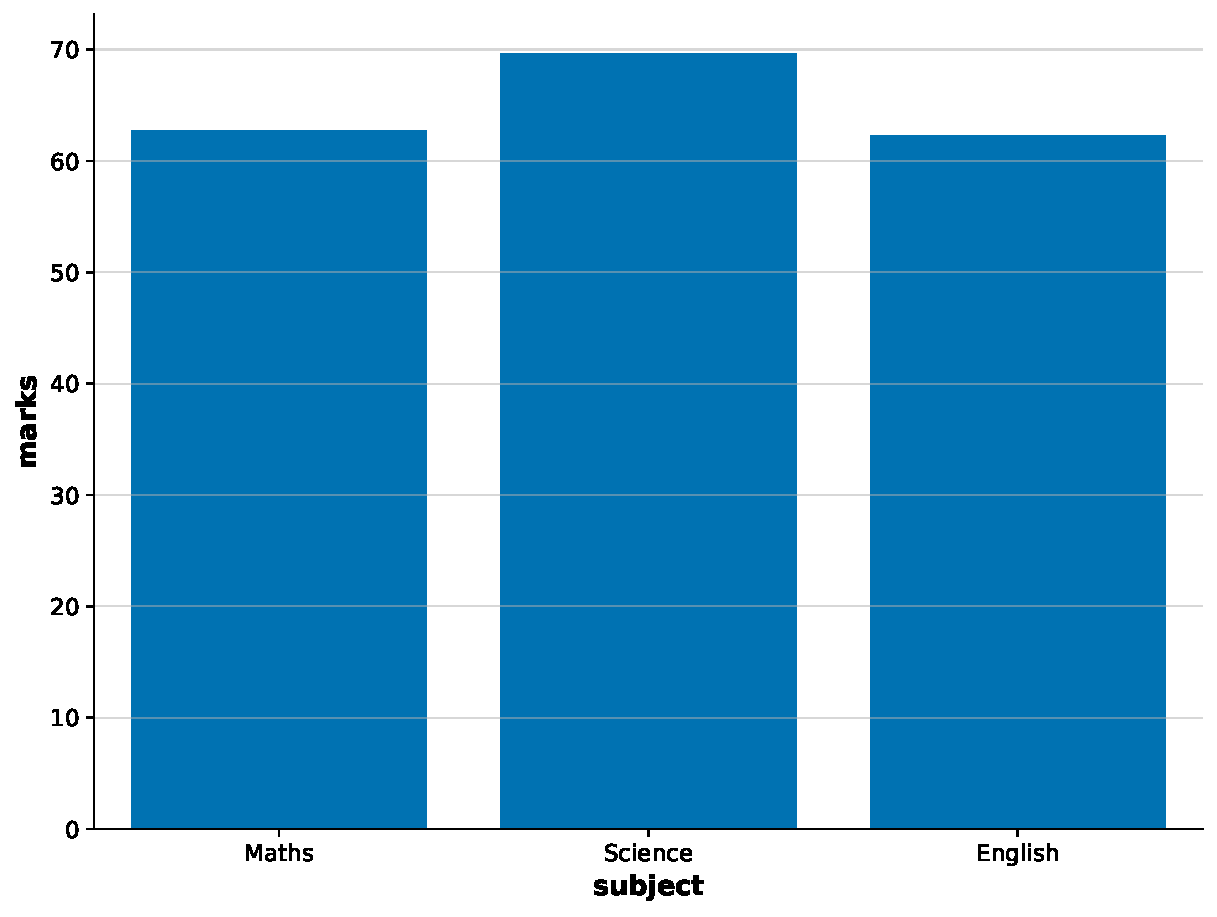
\includegraphics[width=0.52\textwidth,height=0.30\textheight,keepaspectratio]{figures/solution01_task1_lesson1_subjects.pdf}
\captionof*{figure}{Lesson 1, task 1: \code{lesson1\_\allowbreak{}subjects.\allowbreak{}png}.}
\end{minipage}\end{center}
\solutionanswer{Each bar is now one subject, as tall as the average mark of all 18 children in that subject.}
\solutiontask{2}{Save the chart as \code{\textquotedbl{}my\_\allowbreak{}first\_\allowbreak{}chart.\allowbreak{}png\textquotedbl{}} and also as \code{\textquotedbl{}my\_\allowbreak{}first\_\allowbreak{}chart.\allowbreak{}pdf\textquotedbl{}}.}
\begin{lstlisting}[style=py]
import simplydata as sdata
marks = sdata.example("marks")
chart = sdata.chart(marks)
chart.bars(x="name", y="marks")
chart.save("my_first_chart.png")
chart.save("my_first_chart.pdf")
\end{lstlisting}
\printedoutput{output/solution01_task2.txt}
\begin{center}\begin{minipage}{\linewidth}\centering
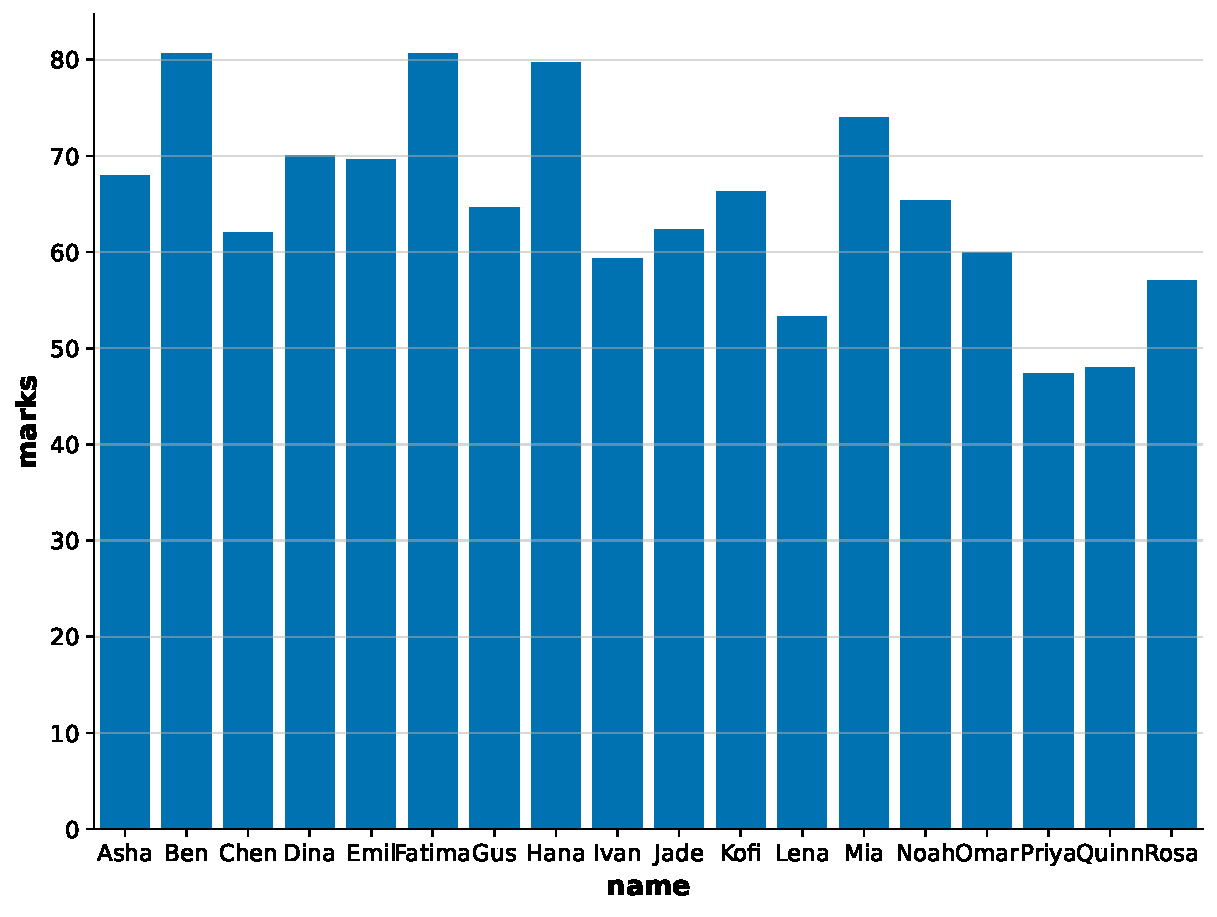
\includegraphics[width=0.52\textwidth,height=0.30\textheight,keepaspectratio]{figures/solution01_task2_my_first_chart.pdf}
\captionof*{figure}{Lesson 1, task 2: \code{my\_\allowbreak{}first\_\allowbreak{}chart.\allowbreak{}png}.}
\end{minipage}\end{center}
\solutionanswer{One chart can be saved many times; the end of the file name (\code{.\allowbreak{}png} or \code{.\allowbreak{}pdf}) decides the type.}
\solutiontask{3}{Make a chart of the \code{\textquotedbl{}fruit\textquotedbl{}} table: bars with \code{x=\textquotedbl{}fruit\textquotedbl{}} and \code{y=\textquotedbl{}count\textquotedbl{}}.}
\begin{lstlisting}[style=py]
import simplydata as sdata
fruit = sdata.example("fruit")
chart = sdata.chart(fruit)
chart.bars(x="fruit", y="count")
chart.save("fruit.png")
\end{lstlisting}
\printedoutput{output/solution01_task3.txt}
\begin{center}\begin{minipage}{\linewidth}\centering
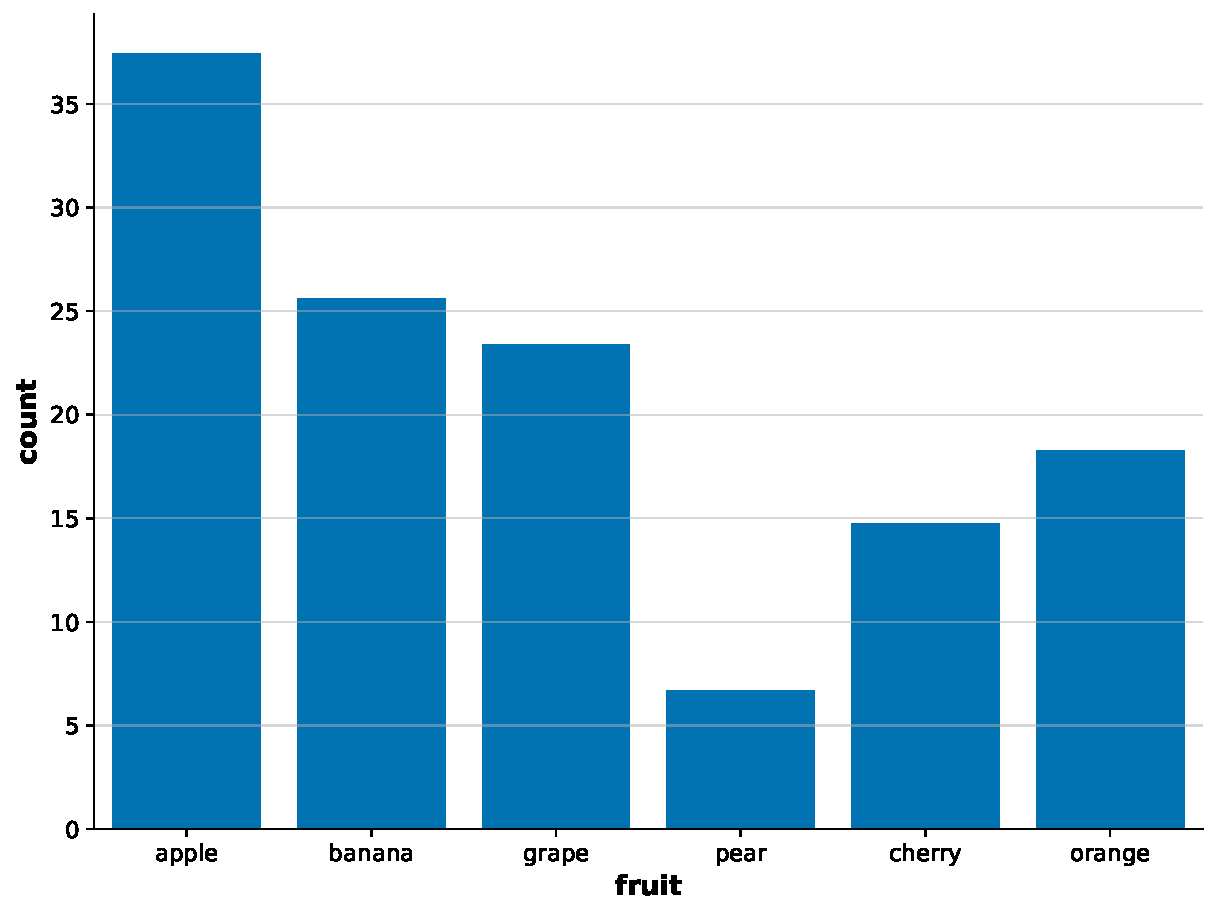
\includegraphics[width=0.52\textwidth,height=0.30\textheight,keepaspectratio]{figures/solution01_task3_fruit.pdf}
\captionof*{figure}{Lesson 1, task 3: \code{fruit.\allowbreak{}png}.}
\end{minipage}\end{center}
\solutionanswer{One bar per fruit. Each fruit was sold several times, so a bar is the average count of one sale; \code{show=\textquotedbl{}total\textquotedbl{}} would show how many were sold in the whole week.}
\par\noindent{\small\sffamily\hyperref[lesson:1]{Back to lesson 1}}
\unsection{Lesson 2: Titles and labels}{solutions:2}
\solutiontask{1}{Give the chart your own title, and label the y-axis \code{\textquotedbl{}Marks out of 100\textquotedbl{}}.}
\begin{lstlisting}[style=py]
import simplydata as sdata
marks = sdata.example("marks")
chart = sdata.chart(marks)
chart.bars(x="name", y="marks")
chart.title_top("How well did each child do?")
chart.label_y("Marks out of 100")
chart.rotate_labels_x(45)
chart.save("lesson2_my_title.png")
\end{lstlisting}
\printedoutput{output/solution02_task1.txt}
\begin{center}\begin{minipage}{\linewidth}\centering
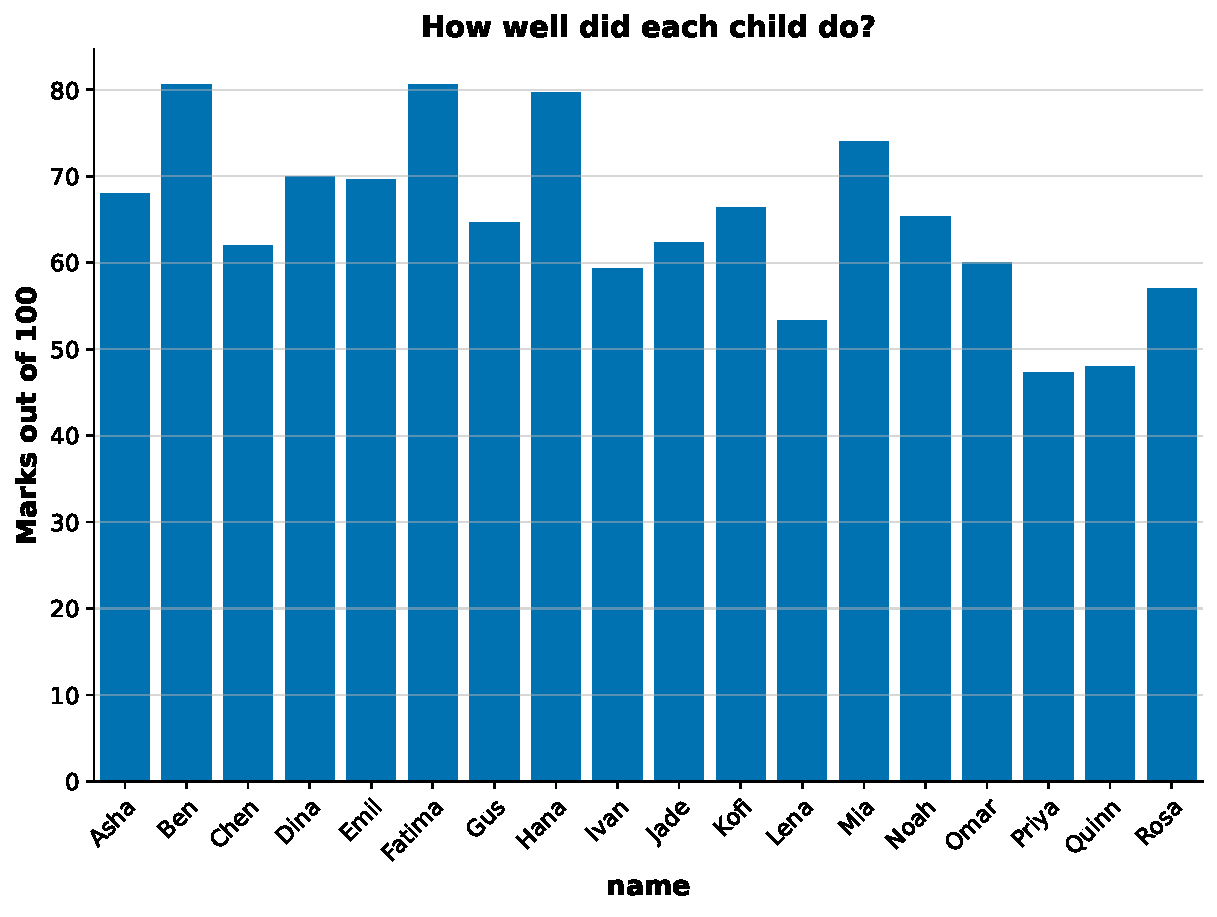
\includegraphics[width=0.52\textwidth,height=0.30\textheight,keepaspectratio]{figures/solution02_task1_lesson2_my_title.pdf}
\captionof*{figure}{Lesson 2, task 1: \code{lesson2\_\allowbreak{}my\_\allowbreak{}title.\allowbreak{}png}.}
\end{minipage}\end{center}
\solutionanswer{\code{title\_\allowbreak{}top} writes any title you like, and \code{label\_\allowbreak{}y} names the y-axis.}
\solutiontask{2}{Try \code{chart.\allowbreak{}font\_\allowbreak{}size(20)}. Then try 9. Which is easier to read?}
\begin{lstlisting}[style=py]
import simplydata as sdata
marks = sdata.example("marks")
chart = sdata.chart(marks)
chart.bars(x="name", y="marks")
chart.title_top("Our class marks")
chart.rotate_labels_x(45)
chart.font_size(20)
chart.save("lesson2_big_text.png")
chart.font_size(9)
chart.save("lesson2_small_text.png")
\end{lstlisting}
\printedoutput{output/solution02_task2.txt}
\begin{center}\begin{minipage}{\linewidth}\centering
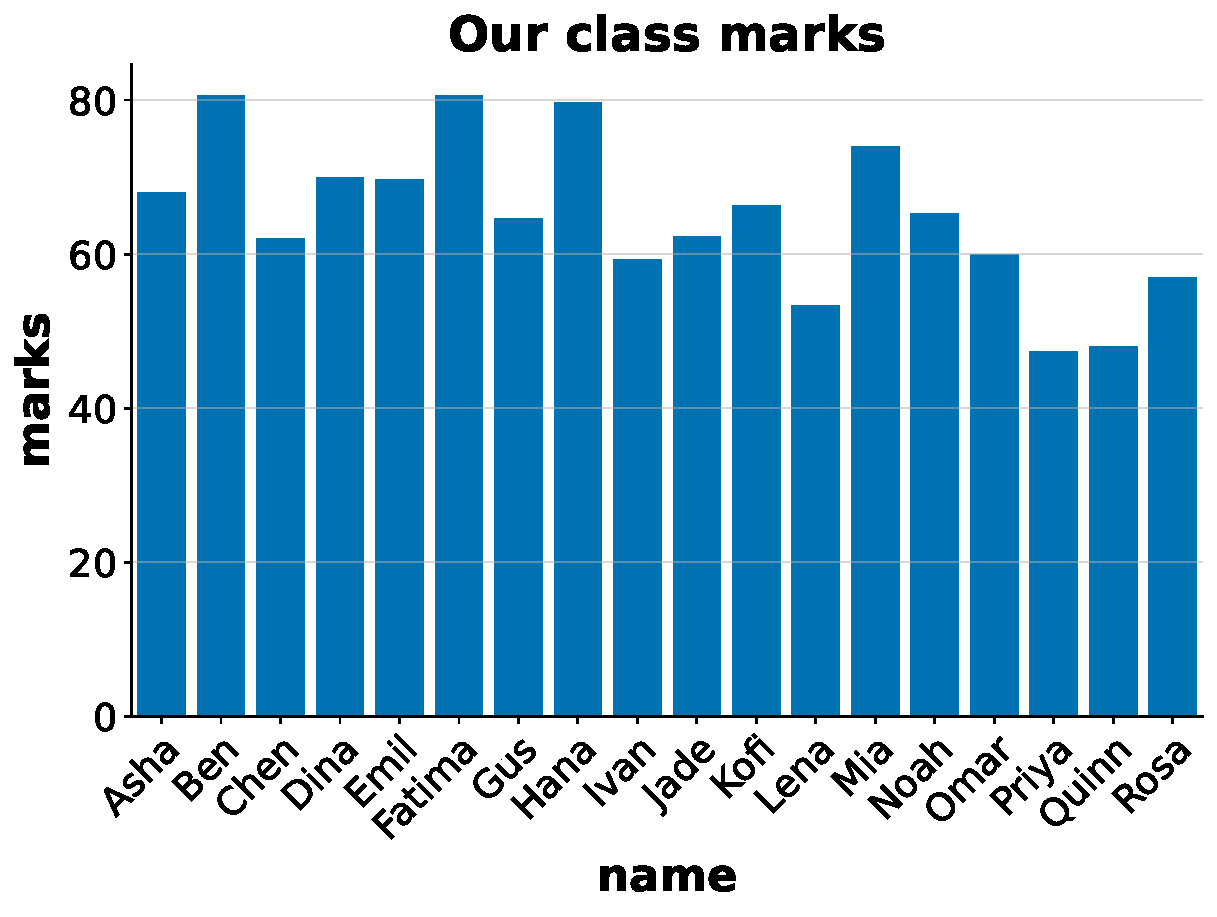
\includegraphics[width=0.48\textwidth,height=0.30\textheight,keepaspectratio]{figures/solution02_task2_lesson2_big_text.pdf}\hfill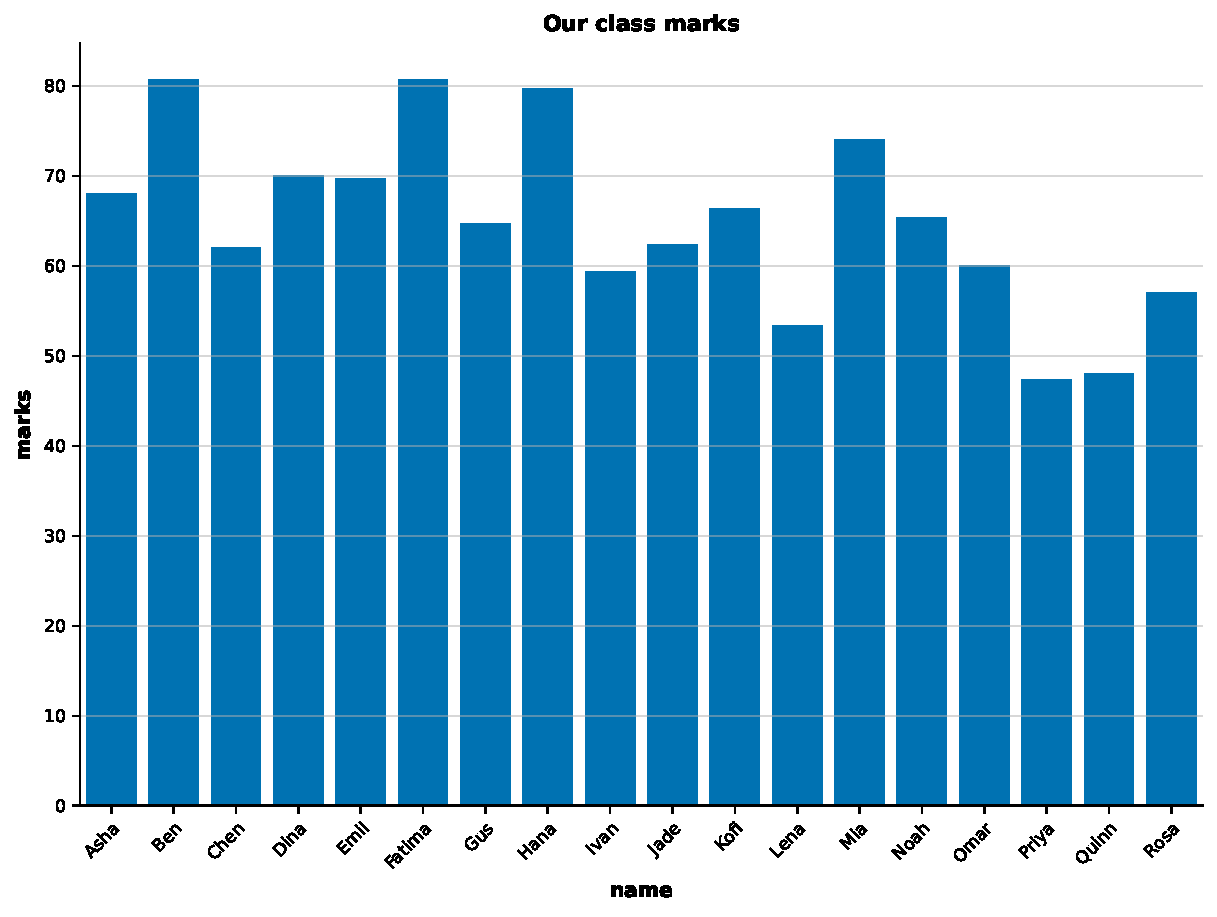
\includegraphics[width=0.48\textwidth,height=0.30\textheight,keepaspectratio]{figures/solution02_task2_lesson2_small_text.pdf}
\captionof*{figure}{Lesson 2, task 2: \code{lesson2\_\allowbreak{}big\_\allowbreak{}text.\allowbreak{}png} and \code{lesson2\_\allowbreak{}small\_\allowbreak{}text.\allowbreak{}png}.}
\end{minipage}\end{center}
\solutionanswer{The last \code{font\_\allowbreak{}size} wins, so one chart gives both pictures. Size 20 is easy to read on a slide but crowds the names; 9 fits everything but is small. 12 to 14 suits most charts.}
\solutiontask{3}{Take away the line \code{chart.\allowbreak{}rotate\_\allowbreak{}labels\_\allowbreak{}x(45)}. What happens to the names?}
\begin{lstlisting}[style=py]
import simplydata as sdata
marks = sdata.example("marks")
chart = sdata.chart(marks)
chart.bars(x="name", y="marks")
chart.title_top("Our class marks")
chart.save("lesson2_no_rotate.png")
\end{lstlisting}
\printedoutput{output/solution02_task3.txt}
\begin{center}\begin{minipage}{\linewidth}\centering
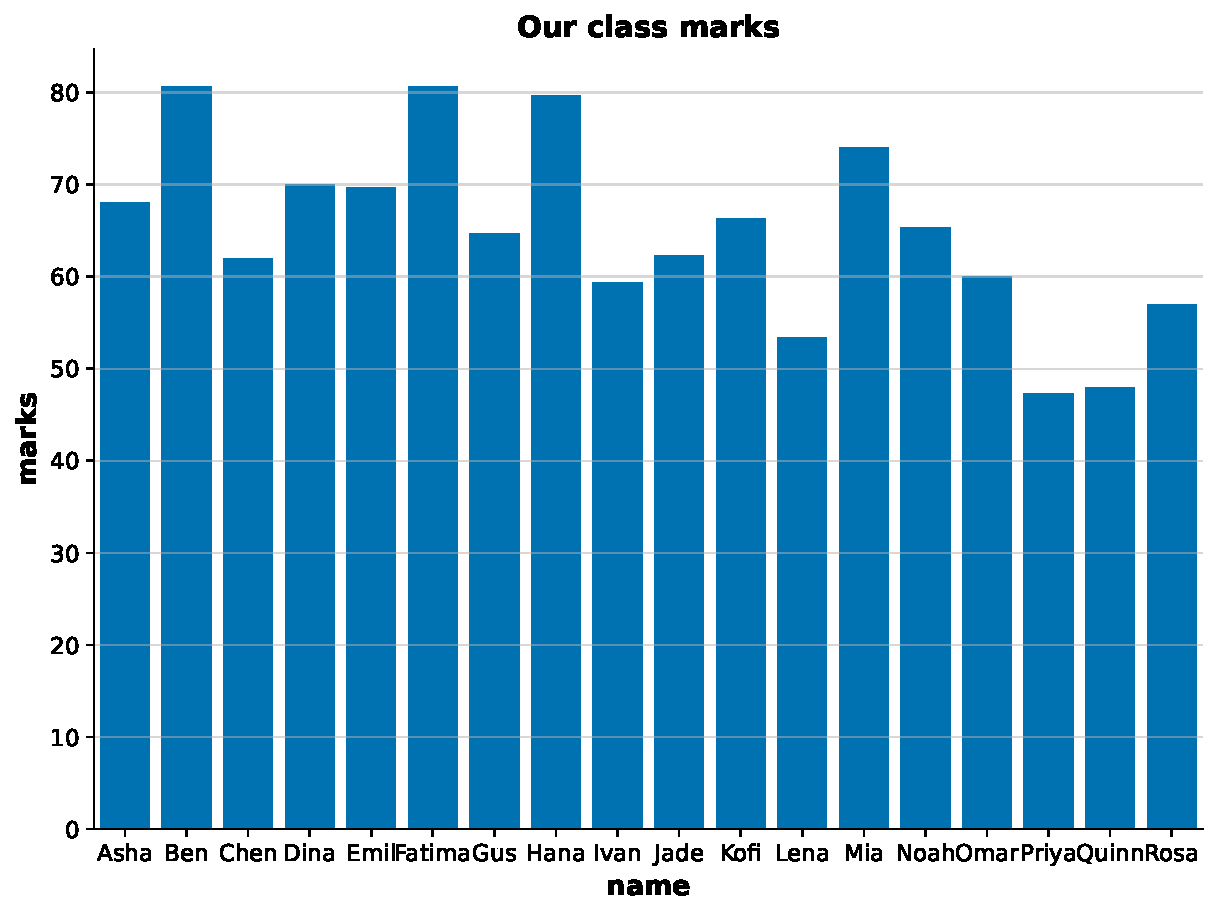
\includegraphics[width=0.52\textwidth,height=0.30\textheight,keepaspectratio]{figures/solution02_task3_lesson2_no_rotate.pdf}
\captionof*{figure}{Lesson 2, task 3: \code{lesson2\_\allowbreak{}no\_\allowbreak{}rotate.\allowbreak{}png}.}
\end{minipage}\end{center}
\solutionanswer{Without \code{rotate\_\allowbreak{}labels\_\allowbreak{}x} the 18 names lie flat under the bars and run into each other.}
\par\noindent{\small\sffamily\hyperref[lesson:2]{Back to lesson 2}}
\unsection{Lesson 3: Colours, groups and legends}{solutions:3}
\solutiontask{1}{In the weather chart, add \code{colour=\textquotedbl{}city\textquotedbl{}} to \code{chart.\allowbreak{}lines(.\allowbreak{}.\allowbreak{}.\allowbreak{})}. How many lines do you get?}
\begin{lstlisting}[style=py]
import simplydata as sdata
weather = sdata.example("weather")
chart = sdata.chart(weather)
chart.lines(x="month", y="rain", colour="city")
chart.save("lesson3_cities.png")
\end{lstlisting}
\printedoutput{output/solution03_task1.txt}
\begin{center}\begin{minipage}{\linewidth}\centering
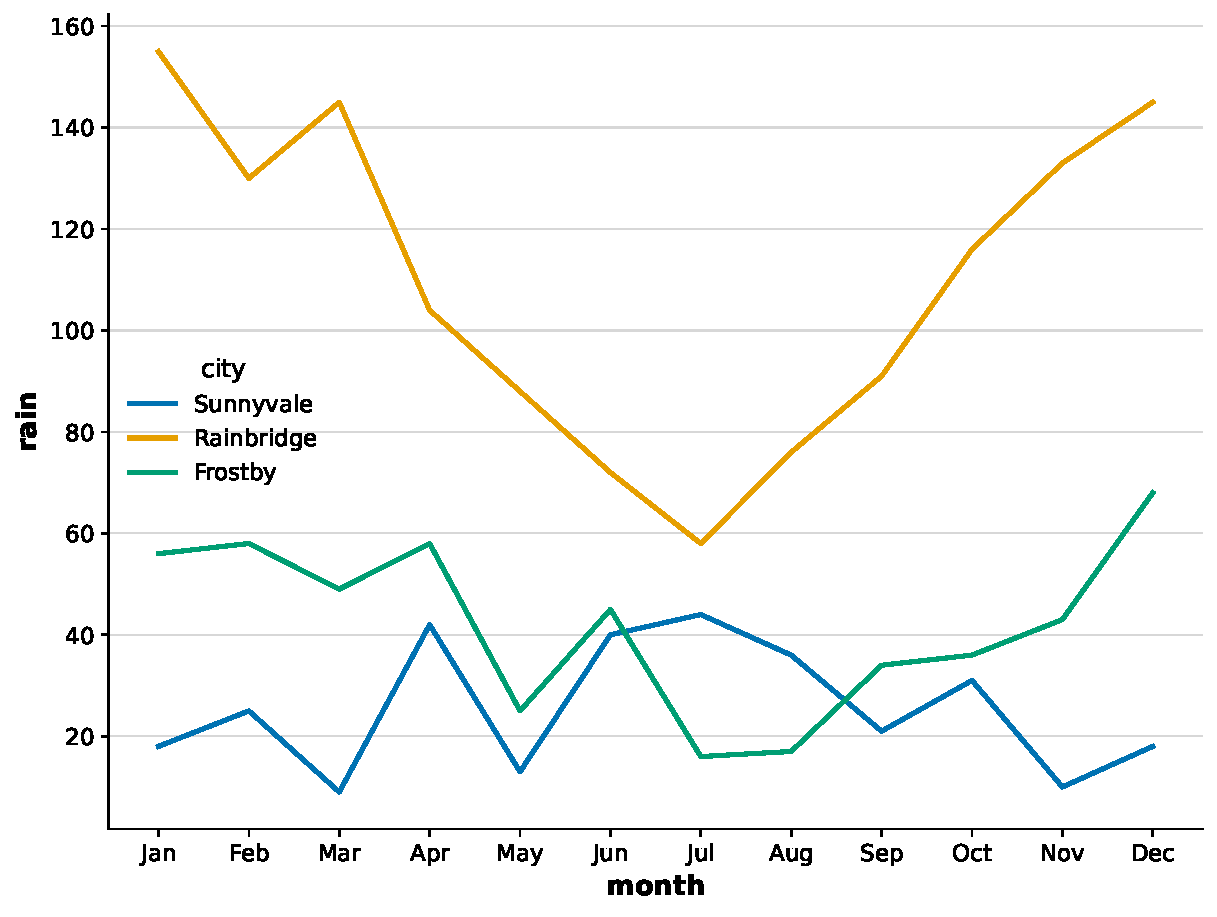
\includegraphics[width=0.52\textwidth,height=0.30\textheight,keepaspectratio]{figures/solution03_task1_lesson3_cities.pdf}
\captionof*{figure}{Lesson 3, task 1: \code{lesson3\_\allowbreak{}cities.\allowbreak{}png}.}
\end{minipage}\end{center}
\solutionanswer{Three lines, one for each city, and a legend that says which colour is which city.}
\solutiontask{2}{Move the legend to the top with \code{chart.\allowbreak{}legend\_\allowbreak{}top()}.}
\begin{lstlisting}[style=py]
import simplydata as sdata
marks = sdata.example("marks")
chart = sdata.chart(marks)
chart.bars(x="subject", y="marks", colour="class")
chart.colours("orange", "teal", "purple")
chart.legend_top()
chart.save("lesson3_legend_top.png")
\end{lstlisting}
\printedoutput{output/solution03_task2.txt}
\begin{center}\begin{minipage}{\linewidth}\centering
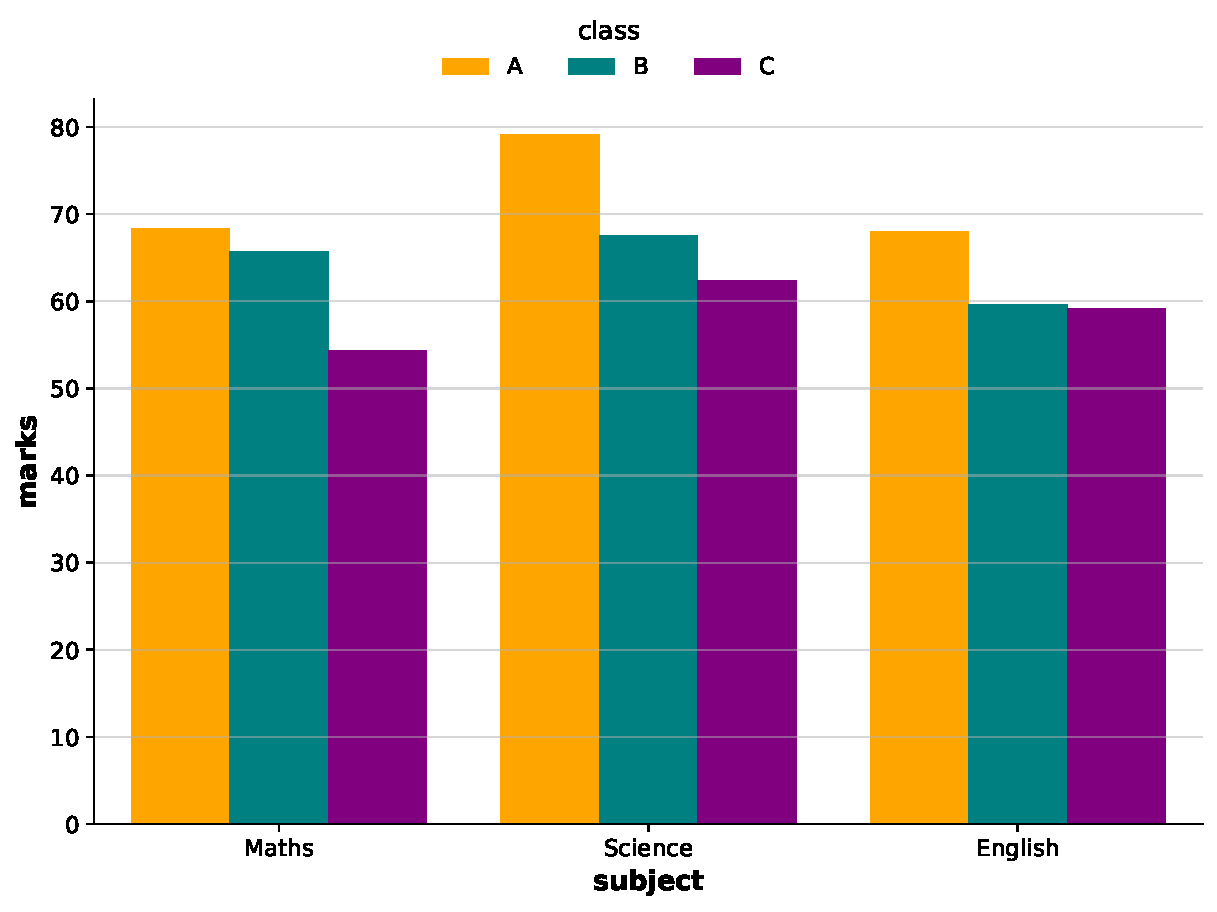
\includegraphics[width=0.52\textwidth,height=0.30\textheight,keepaspectratio]{figures/solution03_task2_lesson3_legend_top.pdf}
\captionof*{figure}{Lesson 3, task 2: \code{lesson3\_\allowbreak{}legend\_\allowbreak{}top.\allowbreak{}png}.}
\end{minipage}\end{center}
\solutionanswer{\code{legend\_\allowbreak{}top} puts the legend above the chart, in place of \code{legend\_\allowbreak{}bottom}.}
\solutiontask{3}{Try \code{chart.\allowbreak{}style(\textquotedbl{}dark\textquotedbl{})} and choose three colours that look good on it.}
\begin{lstlisting}[style=py]
import simplydata as sdata
marks = sdata.example("marks")
chart = sdata.chart(marks)
chart.bars(x="subject", y="marks", colour="class")
chart.style("dark")
chart.colours("gold", "turquoise", "hotpink")
chart.save("lesson3_dark.png")
\end{lstlisting}
\printedoutput{output/solution03_task3.txt}
\begin{center}\begin{minipage}{\linewidth}\centering
\includegraphics[width=0.52\textwidth,height=0.30\textheight,keepaspectratio]{figures/solution03_task3_lesson3_dark.pdf}
\captionof*{figure}{Lesson 3, task 3: \code{lesson3\_\allowbreak{}dark.\allowbreak{}png}.}
\end{minipage}\end{center}
\solutionanswer{Light, bright colours stand out on a dark background; dark colours such as navy would almost disappear.}
\par\noindent{\small\sffamily\hyperref[lesson:3]{Back to lesson 3}}
\unsection{Lesson 4: Different chart types}{solutions:4}
\solutiontask{1}{Draw \code{chart.\allowbreak{}violins(x=\textquotedbl{}class\textquotedbl{},\allowbreak{} y=\textquotedbl{}marks\textquotedbl{})} instead of boxes. What is different?}
\begin{lstlisting}[style=py]
import simplydata as sdata
marks = sdata.example("marks")
chart = sdata.chart(marks)
chart.violins(x="class", y="marks")
chart.all_dots(x="class", y="marks")
chart.save("lesson4_violins.png")
\end{lstlisting}
\printedoutput{output/solution04_task1.txt}
\begin{center}\begin{minipage}{\linewidth}\centering
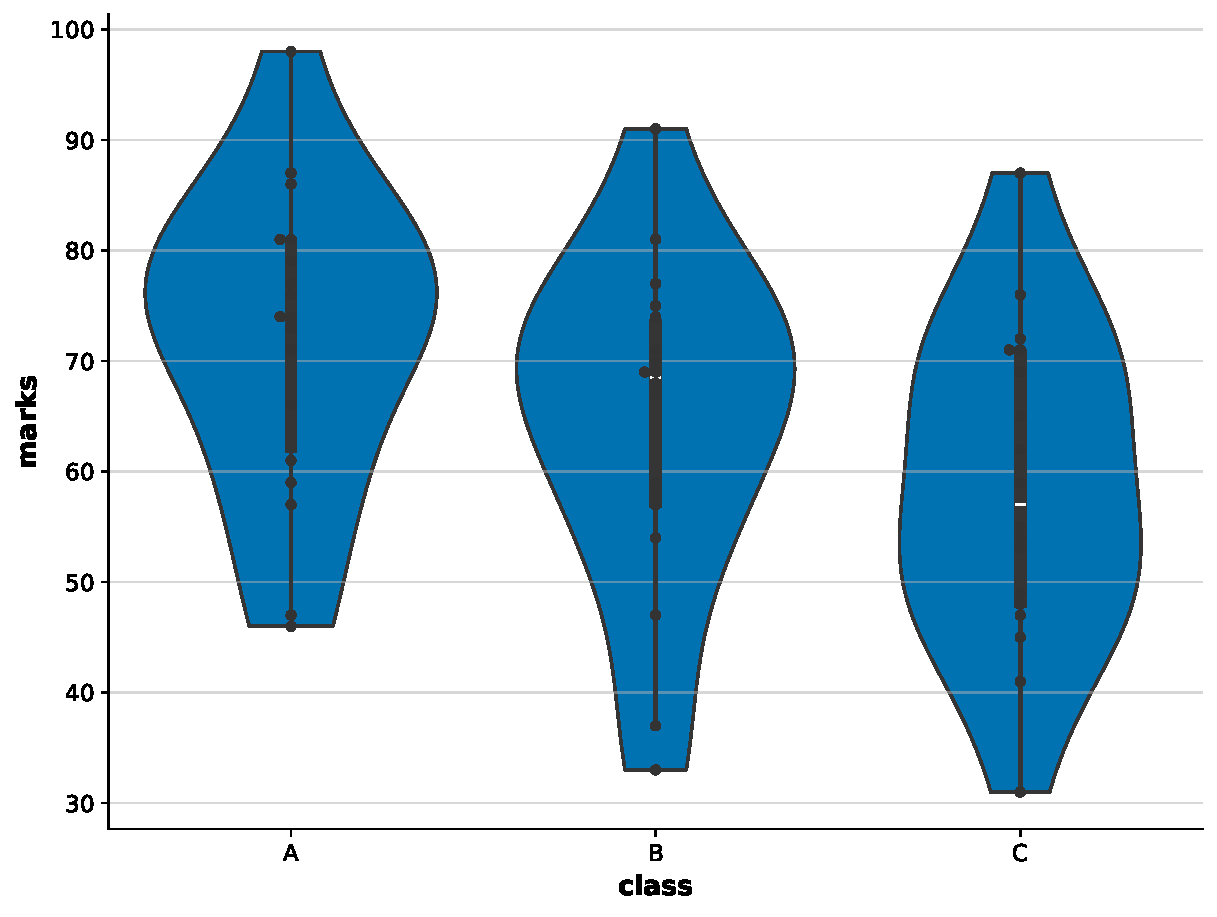
\includegraphics[width=0.52\textwidth,height=0.30\textheight,keepaspectratio]{figures/solution04_task1_lesson4_violins.pdf}
\captionof*{figure}{Lesson 4, task 1: \code{lesson4\_\allowbreak{}violins.\allowbreak{}png}.}
\end{minipage}\end{center}
\solutionanswer{A violin shows the whole shape of the marks: it is wide where many marks are and thin where few are. A box shows only the middle half and the median.}
\solutiontask{2}{Draw a histogram of the weather \code{\textquotedbl{}temperature\textquotedbl{}} column with \code{bins=6}.}
\begin{lstlisting}[style=py]
import simplydata as sdata
weather = sdata.example("weather")
chart = sdata.chart(weather)
chart.histogram(x="temperature", bins=6)
chart.save("lesson4_temperature.png")
\end{lstlisting}
\printedoutput{output/solution04_task2.txt}
\begin{center}\begin{minipage}{\linewidth}\centering
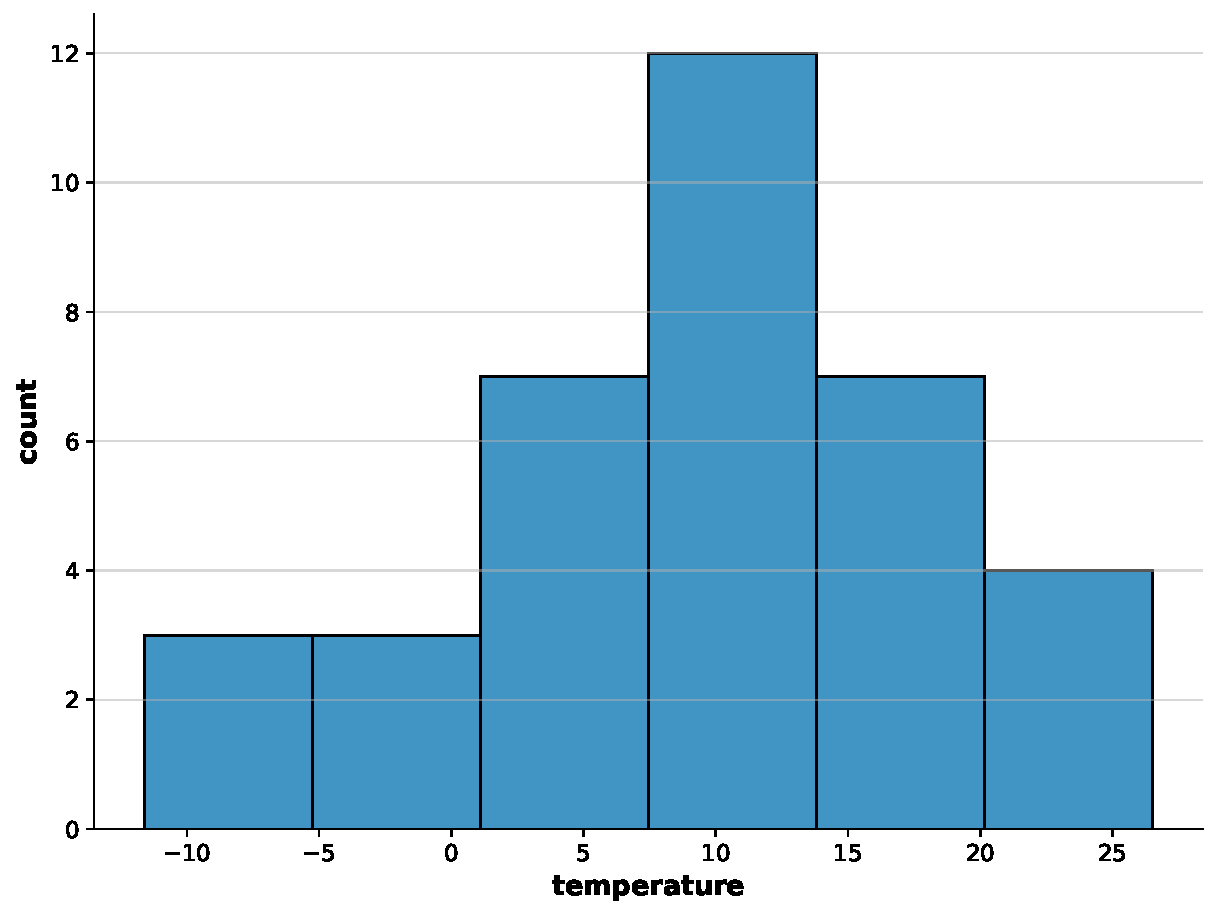
\includegraphics[width=0.52\textwidth,height=0.30\textheight,keepaspectratio]{figures/solution04_task2_lesson4_temperature.pdf}
\captionof*{figure}{Lesson 4, task 2: \code{lesson4\_\allowbreak{}temperature.\allowbreak{}png}.}
\end{minipage}\end{center}
\solutionanswer{Six ranges of temperature, each bar as high as the number of months (of all three cities) that fall in it.}
\solutiontask{3}{Make a chart of \code{sdata.\allowbreak{}example(\textquotedbl{}growth\textquotedbl{})} and draw \code{chart.\allowbreak{}area(x=\textquotedbl{}year\textquotedbl{},\allowbreak{} y=\textquotedbl{}population\textquotedbl{},\allowbreak{} colour=\textquotedbl{}country\textquotedbl{})}.}
\begin{lstlisting}[style=py]
import simplydata as sdata
growth = sdata.example("growth")
chart = sdata.chart(growth)
chart.area(x="year", y="population", colour="country")
chart.save("lesson4_area.png")
\end{lstlisting}
\printedoutput{output/solution04_task3.txt}
\begin{center}\begin{minipage}{\linewidth}\centering
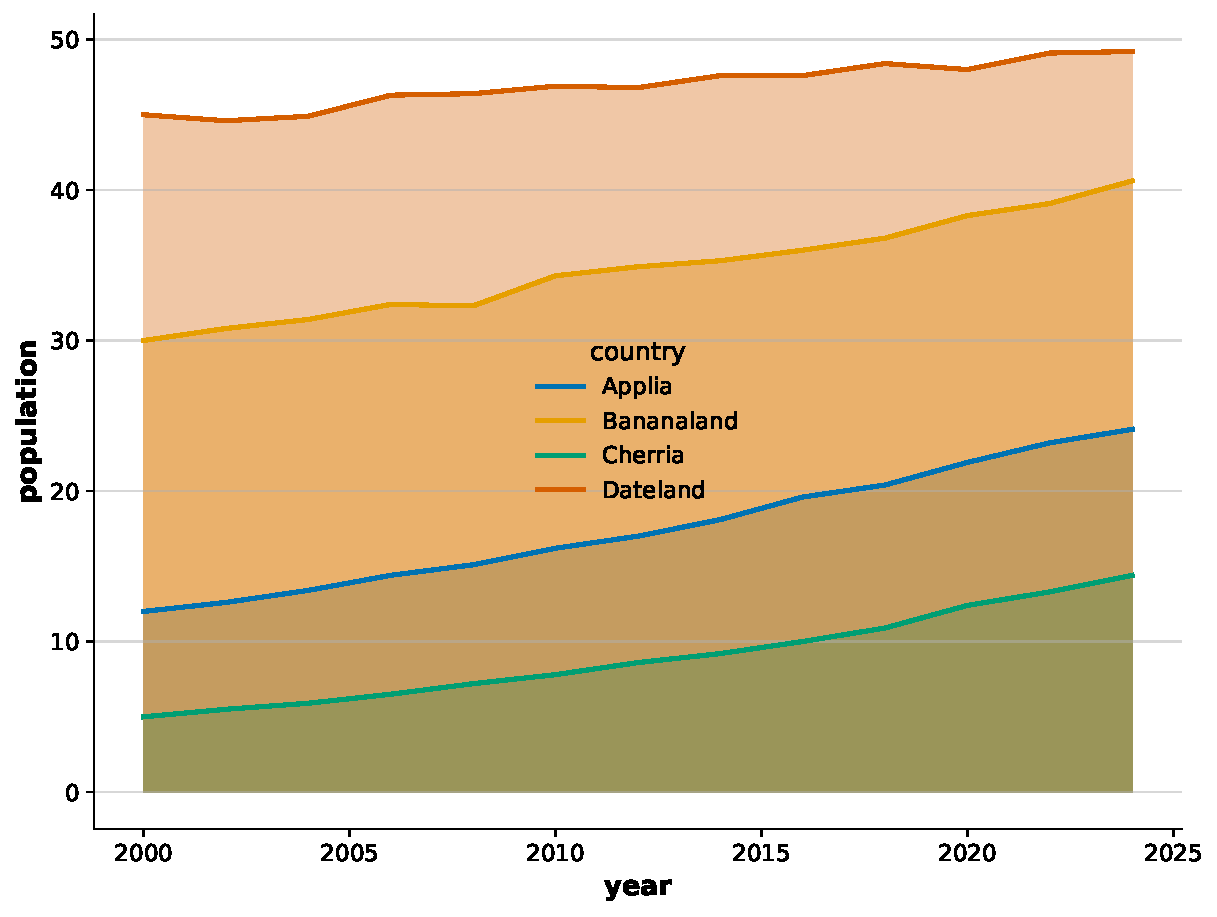
\includegraphics[width=0.52\textwidth,height=0.30\textheight,keepaspectratio]{figures/solution04_task3_lesson4_area.pdf}
\captionof*{figure}{Lesson 4, task 3: \code{lesson4\_\allowbreak{}area.\allowbreak{}png}.}
\end{minipage}\end{center}
\solutionanswer{An area chart is a line chart with the space under each line filled in.}
\par\noindent{\small\sffamily\hyperref[lesson:4]{Back to lesson 4}}
\unsection{Lesson 5: Statistics: averages, error bars and fit lines}{solutions:5}
\solutiontask{1}{Change \code{show=\textquotedbl{}average\textquotedbl{}} to \code{show=\textquotedbl{}median\textquotedbl{}}. Do the bars change much?}
\begin{lstlisting}[style=py]
import simplydata as sdata
marks = sdata.example("marks")
chart = sdata.chart(marks)
chart.bars(x="class", y="marks", show="median")
chart.numbers_on_bars()
chart.save("lesson5_median.png")
\end{lstlisting}
\printedoutput{output/solution05_task1.txt}
\begin{center}\begin{minipage}{\linewidth}\centering
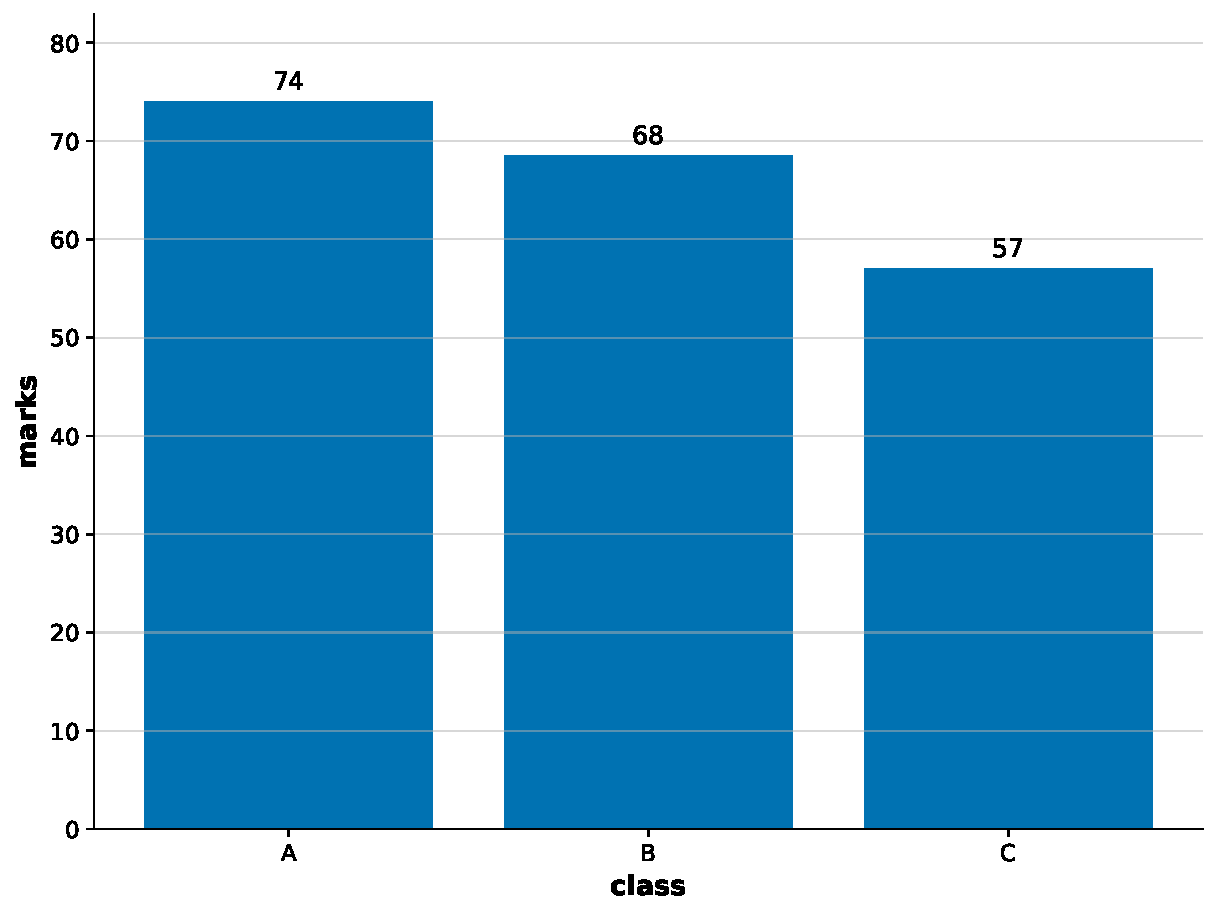
\includegraphics[width=0.52\textwidth,height=0.30\textheight,keepaspectratio]{figures/solution05_task1_lesson5_median.pdf}
\captionof*{figure}{Lesson 5, task 1: \code{lesson5\_\allowbreak{}median.\allowbreak{}png}.}
\end{minipage}\end{center}
\solutionanswer{Error bars go with averages, so \code{error=} comes out. The medians (A 74, B 68.5, C 57) are close to the averages (A 71.8, B 64.3, C 58.6): no single mark pulls them far.}
\solutiontask{2}{Change \code{error=\textquotedbl{}standard deviation\textquotedbl{}} to \code{error=\textquotedbl{}standard error\textquotedbl{}}. Are the error bars bigger or smaller? Why?}
\begin{lstlisting}[style=py]
import simplydata as sdata
marks = sdata.example("marks")
chart = sdata.chart(marks)
chart.bars(x="class", y="marks", show="average", error="standard error")
chart.save("lesson5_standard_error.png")
\end{lstlisting}
\printedoutput{output/solution05_task2.txt}
\begin{center}\begin{minipage}{\linewidth}\centering
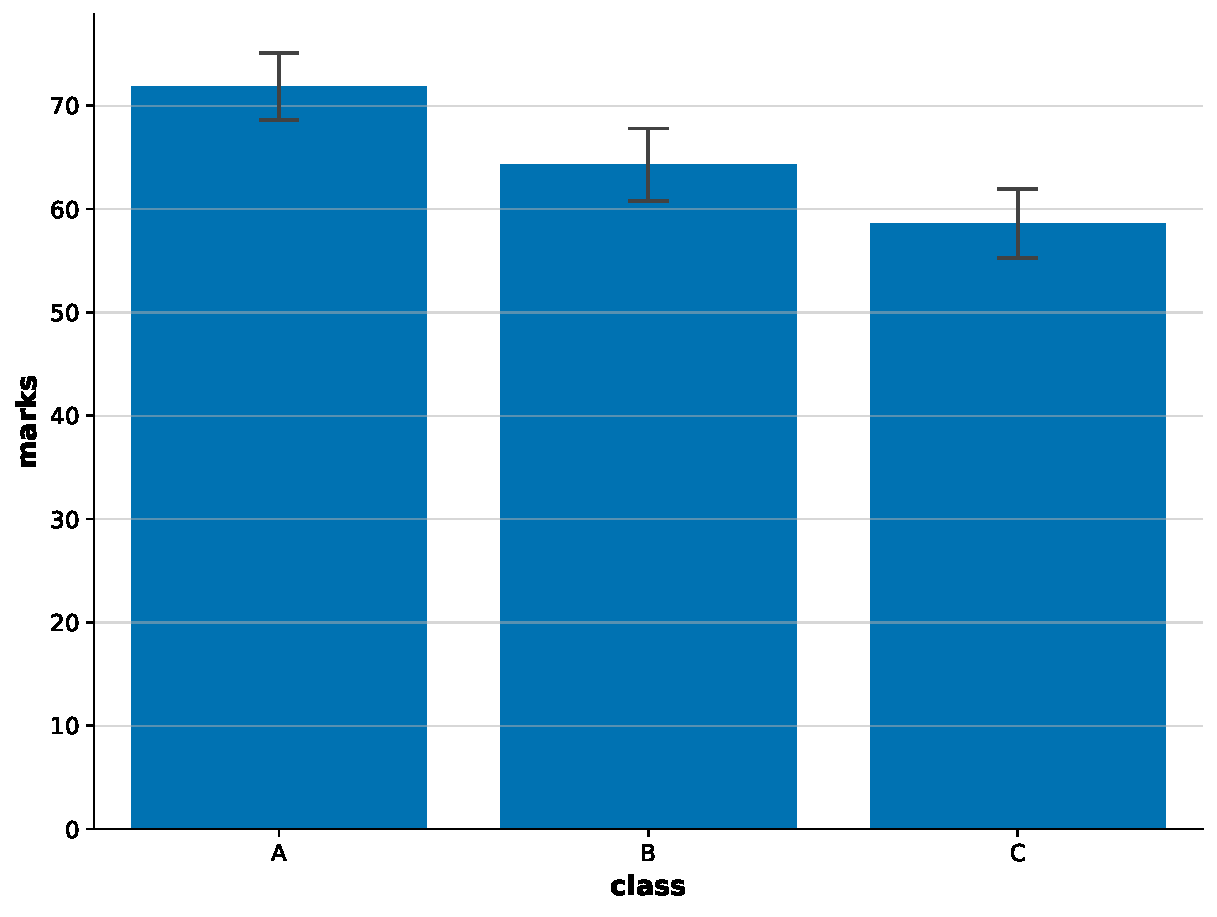
\includegraphics[width=0.52\textwidth,height=0.30\textheight,keepaspectratio]{figures/solution05_task2_lesson5_standard_error.pdf}
\captionof*{figure}{Lesson 5, task 2: \code{lesson5\_\allowbreak{}standard\_\allowbreak{}error.\allowbreak{}png}.}
\end{minipage}\end{center}
\solutionanswer{Smaller: the standard error is the standard deviation divided by the square root of the number of values (here 18), so it is about a quarter of the standard deviation.}
\solutiontask{3}{Make a chart of the weather table, draw dots with \code{x=\textquotedbl{}month\_\allowbreak{}number\textquotedbl{}}, \code{y=\textquotedbl{}temperature\textquotedbl{}} and add \code{chart.\allowbreak{}fit\_\allowbreak{}curve(degree=2)}.}
\begin{lstlisting}[style=py]
import simplydata as sdata
weather = sdata.example("weather")
chart = sdata.chart(weather)
chart.dots(x="month_number", y="temperature", colour="city")
chart.fit_curve(degree=2)
chart.save("lesson5_fit_curve.png")
\end{lstlisting}
\printedoutput{output/solution05_task3.txt}
\begin{center}\begin{minipage}{\linewidth}\centering
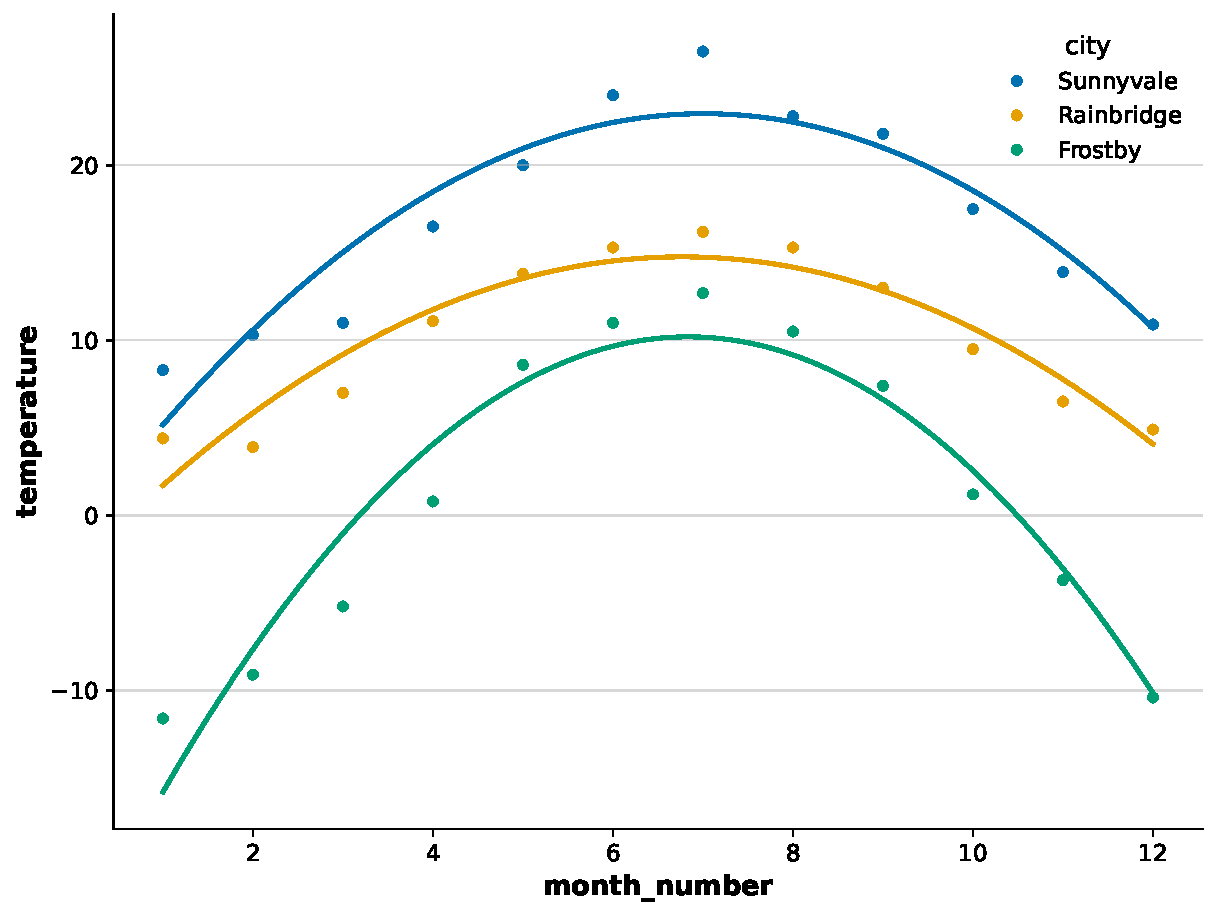
\includegraphics[width=0.52\textwidth,height=0.30\textheight,keepaspectratio]{figures/solution05_task3_lesson5_fit_curve.pdf}
\captionof*{figure}{Lesson 5, task 3: \code{lesson5\_\allowbreak{}fit\_\allowbreak{}curve.\allowbreak{}png}.}
\end{minipage}\end{center}
\solutionanswer{Each city gets a curve with one bend: warm in the middle of the year, cold at both ends.}
\par\noindent{\small\sffamily\hyperref[lesson:5]{Back to lesson 5}}
\unsection{Lesson 6: Axes and reference lines}{solutions:6}
\solutiontask{1}{Move the pass mark to 60 and shade between 0 and 40 instead.}
\begin{lstlisting}[style=py]
import simplydata as sdata
marks = sdata.example("marks")
chart = sdata.chart(marks)
chart.bars(x="name", y="marks")
chart.range_y(0, 100)
chart.line_at_y(60, label="pass mark")
chart.shade_between_y(0, 40)
chart.rotate_labels_x()
chart.save("lesson6_pass_60.png")
\end{lstlisting}
\printedoutput{output/solution06_task1.txt}
\begin{center}\begin{minipage}{\linewidth}\centering
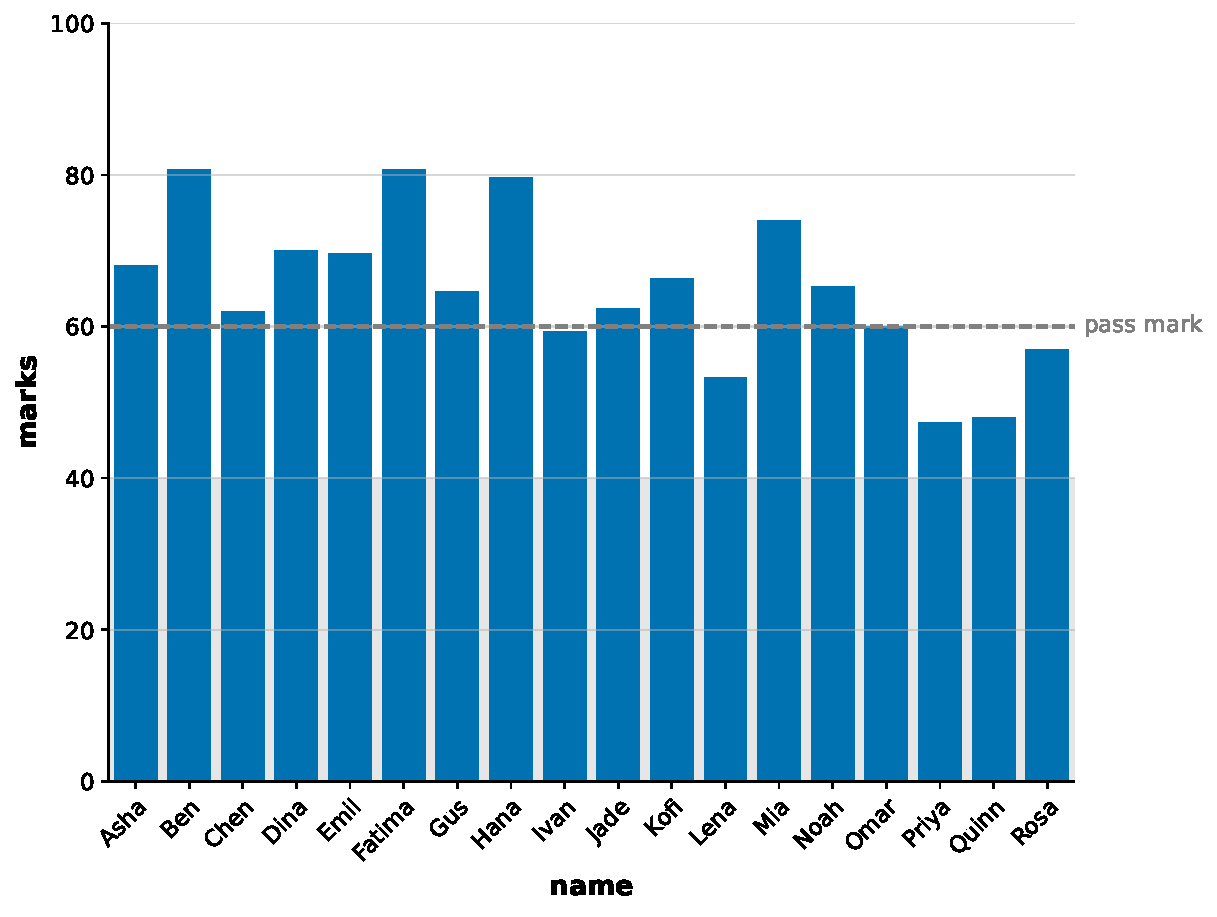
\includegraphics[width=0.52\textwidth,height=0.30\textheight,keepaspectratio]{figures/solution06_task1_lesson6_pass_60.pdf}
\captionof*{figure}{Lesson 6, task 1: \code{lesson6\_\allowbreak{}pass\_\allowbreak{}60.\allowbreak{}png}.}
\end{minipage}\end{center}
\solutionanswer{\code{line\_\allowbreak{}at\_\allowbreak{}y(60)} moves the line; \code{shade\_\allowbreak{}between\_\allowbreak{}y(0,\allowbreak{} 40)} shades the band from 0 to 40.}
\solutiontask{2}{Take away \code{chart.\allowbreak{}log\_\allowbreak{}scale\_\allowbreak{}y()}. Which countries look different?}
\begin{lstlisting}[style=py]
import simplydata as sdata
growth = sdata.example("growth")
chart = sdata.chart(growth)
chart.lines(x="year", y="population", colour="country")
chart.line_at_x(2010, label="2010")
chart.label_y("People (millions)")
chart.save("lesson6_no_log.png")
\end{lstlisting}
\printedoutput{output/solution06_task2.txt}
\begin{center}\begin{minipage}{\linewidth}\centering
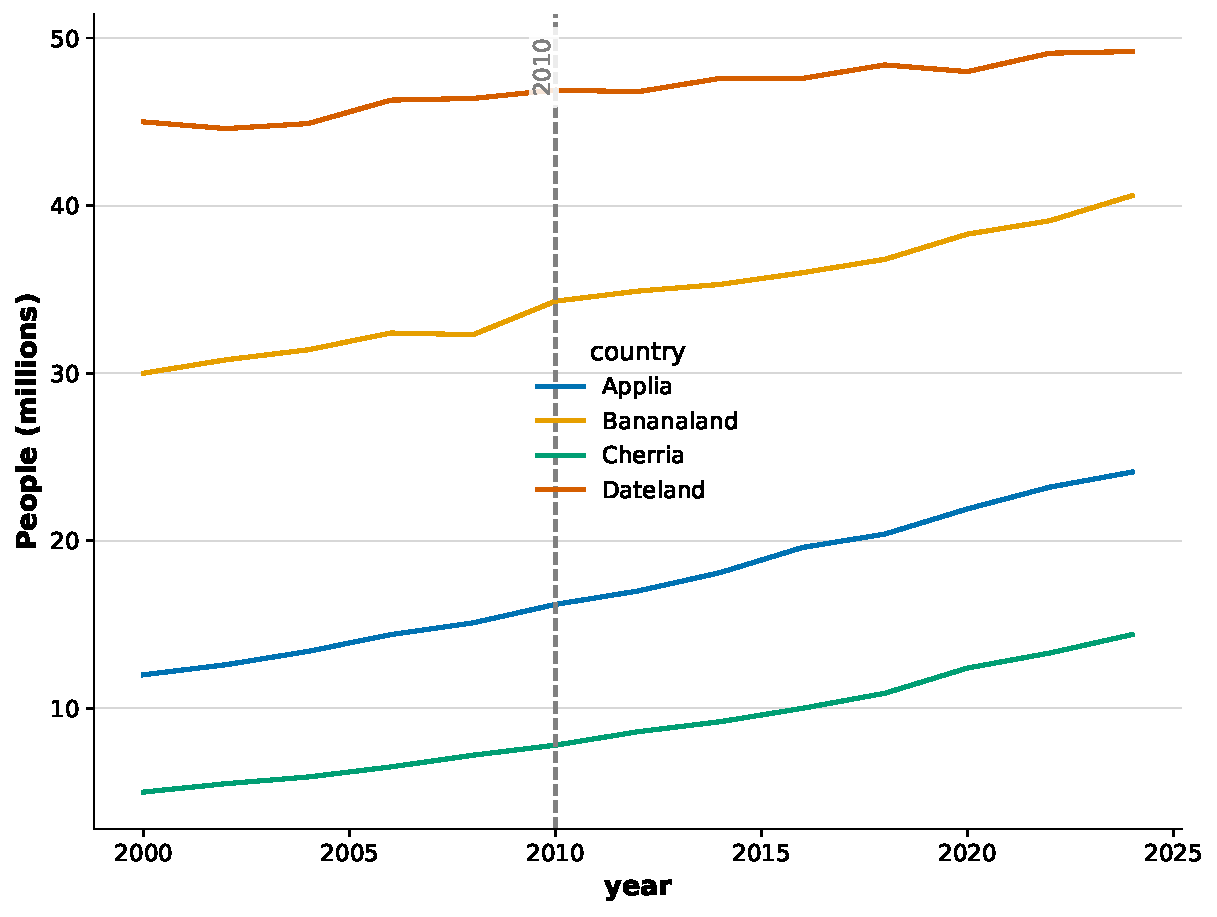
\includegraphics[width=0.52\textwidth,height=0.30\textheight,keepaspectratio]{figures/solution06_task2_lesson6_no_log.pdf}
\captionof*{figure}{Lesson 6, task 2: \code{lesson6\_\allowbreak{}no\_\allowbreak{}log.\allowbreak{}png}.}
\end{minipage}\end{center}
\solutionanswer{The lines now bend upwards instead of running straight, and the small countries (Cherria and Applia) sit low and look flat, although Cherria nearly triples.}
\solutiontask{3}{Try \code{chart.\allowbreak{}flip\_\allowbreak{}y()} on any chart. What happens?}
\begin{lstlisting}[style=py]
import simplydata as sdata
marks = sdata.example("marks")
chart = sdata.chart(marks)
chart.bars(x="class", y="marks")
chart.flip_y()
chart.save("lesson6_flip.png")
\end{lstlisting}
\printedoutput{output/solution06_task3.txt}
\begin{center}\begin{minipage}{\linewidth}\centering
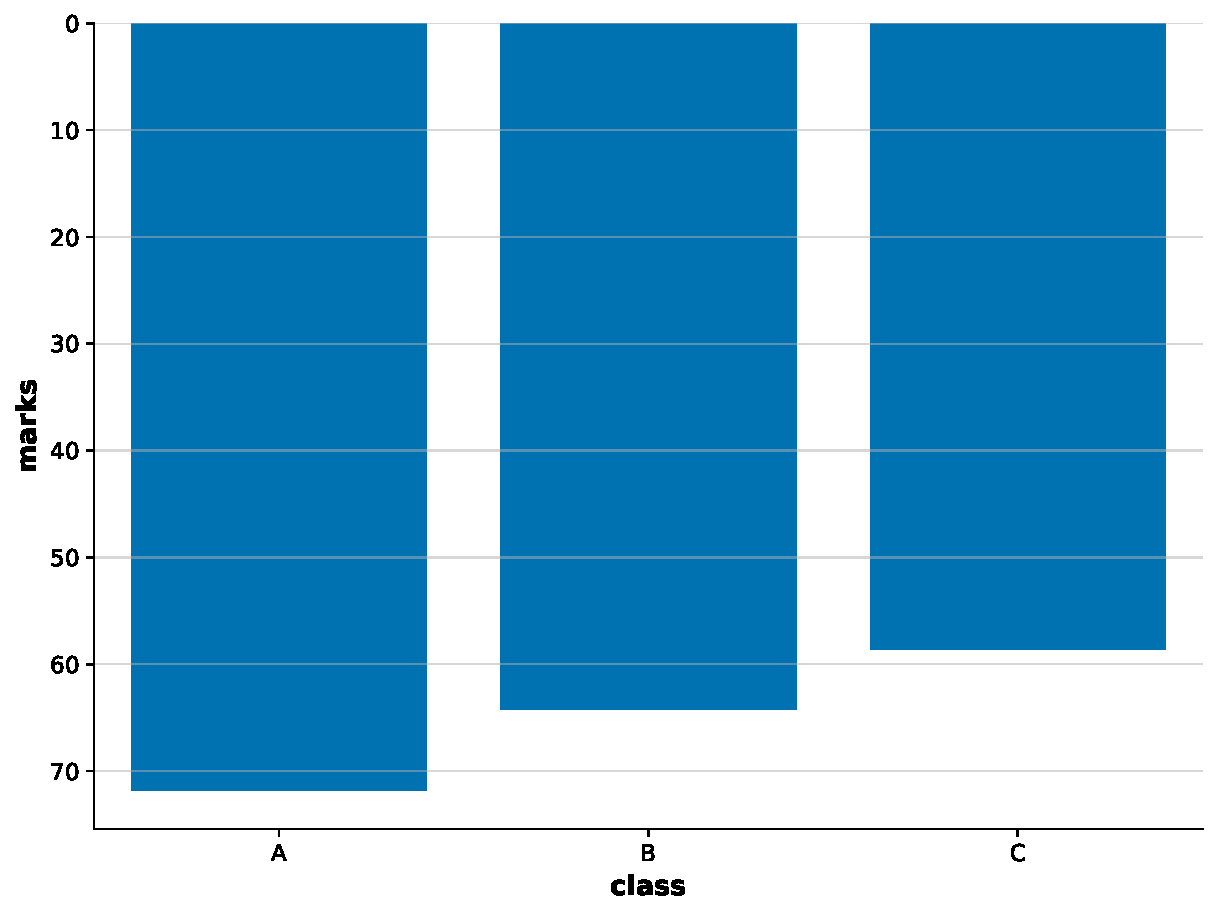
\includegraphics[width=0.52\textwidth,height=0.30\textheight,keepaspectratio]{figures/solution06_task3_lesson6_flip.pdf}
\captionof*{figure}{Lesson 6, task 3: \code{lesson6\_\allowbreak{}flip.\allowbreak{}png}.}
\end{minipage}\end{center}
\solutionanswer{The y-axis turns upside down: 0 is at the top and the bars hang down. Useful for depths, where bigger numbers are further down.}
\par\noindent{\small\sffamily\hyperref[lesson:6]{Back to lesson 6}}
\unsection{Lesson 7: Several charts together}{solutions:7}
\solutiontask{1}{Change \code{chart.\allowbreak{}one\_\allowbreak{}chart\_\allowbreak{}per(\textquotedbl{}class\textquotedbl{})} to \code{chart.\allowbreak{}one\_\allowbreak{}chart\_\allowbreak{}per(\textquotedbl{}subject\textquotedbl{})}.}
\begin{lstlisting}[style=py]
import simplydata as sdata
marks = sdata.example("marks")
chart = sdata.chart(marks)
chart.dots(x="hours", y="marks")
chart.fit_line()
chart.one_chart_per("subject")
chart.save("lesson7_per_subject.png")
\end{lstlisting}
\printedoutput{output/solution07_task1.txt}
\begin{center}\begin{minipage}{\linewidth}\centering
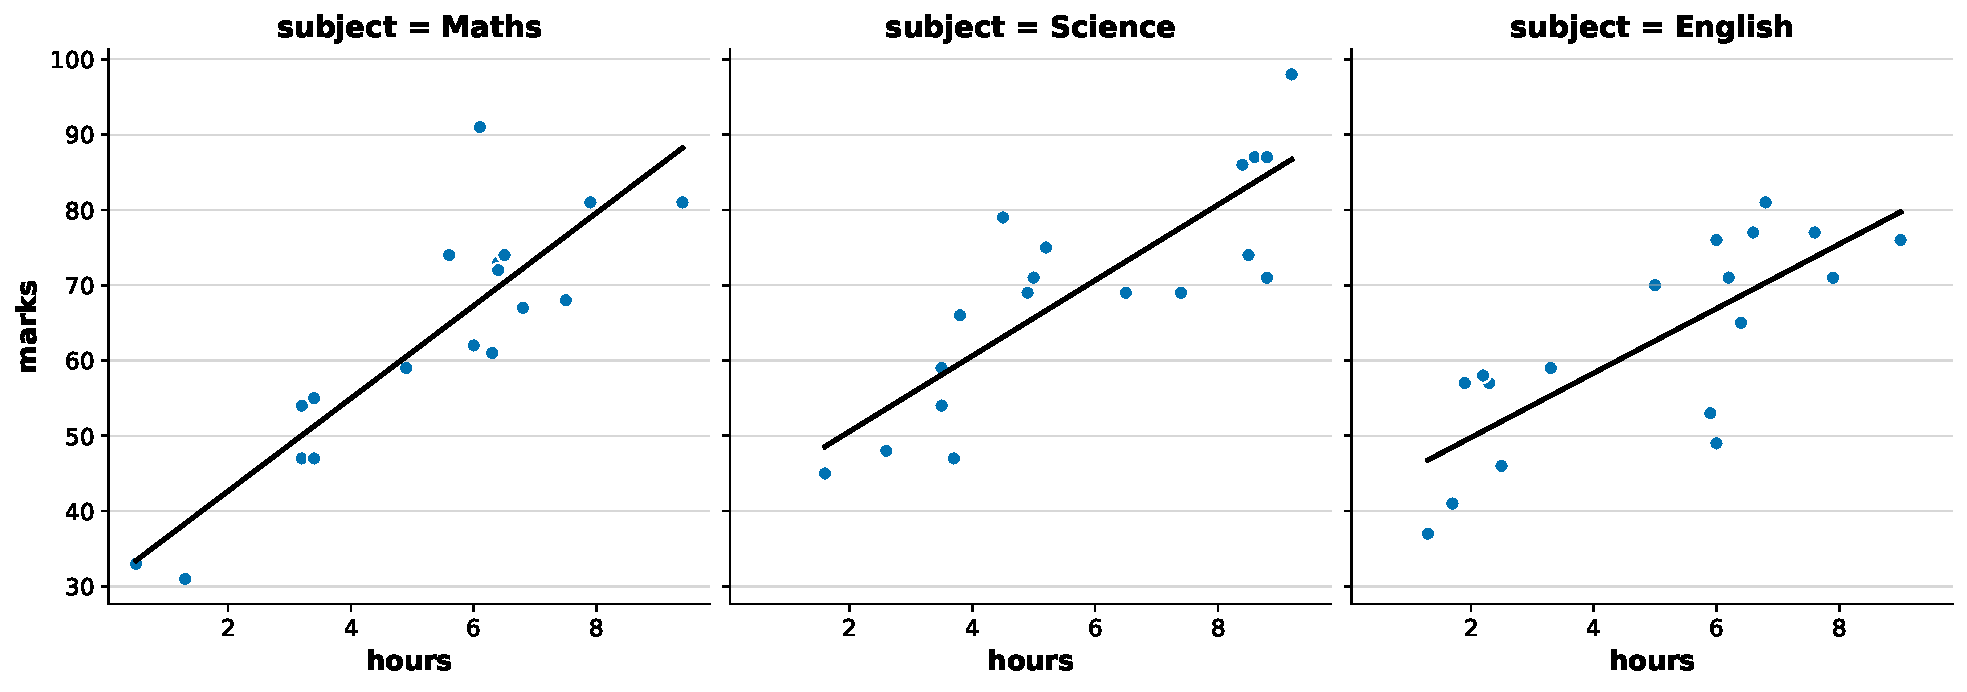
\includegraphics[width=0.52\textwidth,height=0.30\textheight,keepaspectratio]{figures/solution07_task1_lesson7_per_subject.pdf}
\captionof*{figure}{Lesson 7, task 1: \code{lesson7\_\allowbreak{}per\_\allowbreak{}subject.\allowbreak{}png}.}
\end{minipage}\end{center}
\solutionanswer{One small chart for each subject (Maths, Science and English), each with its own fit line.}
\solutiontask{2}{Use \code{sdata.\allowbreak{}side\_\allowbreak{}by\_\allowbreak{}side(a,\allowbreak{} b)} instead of \code{sdata.\allowbreak{}one\_\allowbreak{}above\_\allowbreak{}other(a,\allowbreak{} b)} for the weather charts.}
\begin{lstlisting}[style=py]
import simplydata as sdata
weather = sdata.example("weather")
a = sdata.chart(weather).lines(x="month", y="temperature", colour="city")
b = sdata.chart(weather).bars(x="month", y="rain", colour="city")
page = sdata.side_by_side(a, b)
page.title_top("A year of weather")
page.save("lesson7_side_by_side.png")
\end{lstlisting}
\printedoutput{output/solution07_task2.txt}
\begin{center}\begin{minipage}{\linewidth}\centering
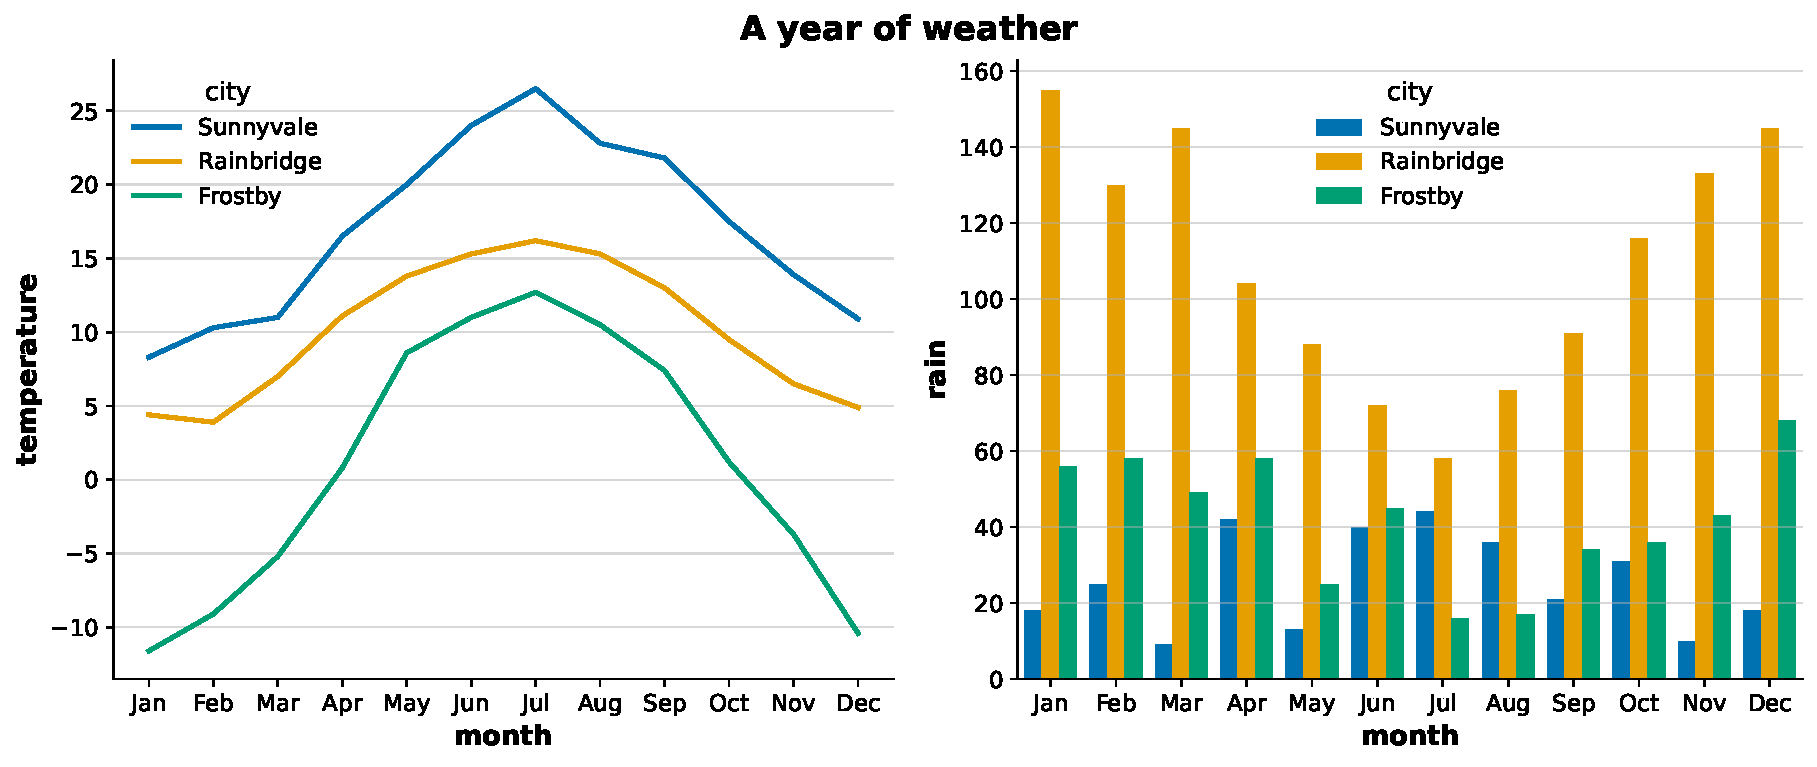
\includegraphics[width=0.52\textwidth,height=0.30\textheight,keepaspectratio]{figures/solution07_task2_lesson7_side_by_side.pdf}
\captionof*{figure}{Lesson 7, task 2: \code{lesson7\_\allowbreak{}side\_\allowbreak{}by\_\allowbreak{}side.\allowbreak{}png}.}
\end{minipage}\end{center}
\solutionanswer{The same two charts, now next to each other instead of one above the other.}
\solutiontask{3}{Make \code{sdata.\allowbreak{}pairs} of \code{sdata.\allowbreak{}example(\textquotedbl{}weather\textquotedbl{})} with \code{colour=\textquotedbl{}city\textquotedbl{}}.}
\begin{lstlisting}[style=py]
import simplydata as sdata
pairs = sdata.pairs(sdata.example("weather"), colour="city")
pairs.save("lesson7_weather_pairs.png")
\end{lstlisting}
\printedoutput{output/solution07_task3.txt}
\begin{center}\begin{minipage}{\linewidth}\centering
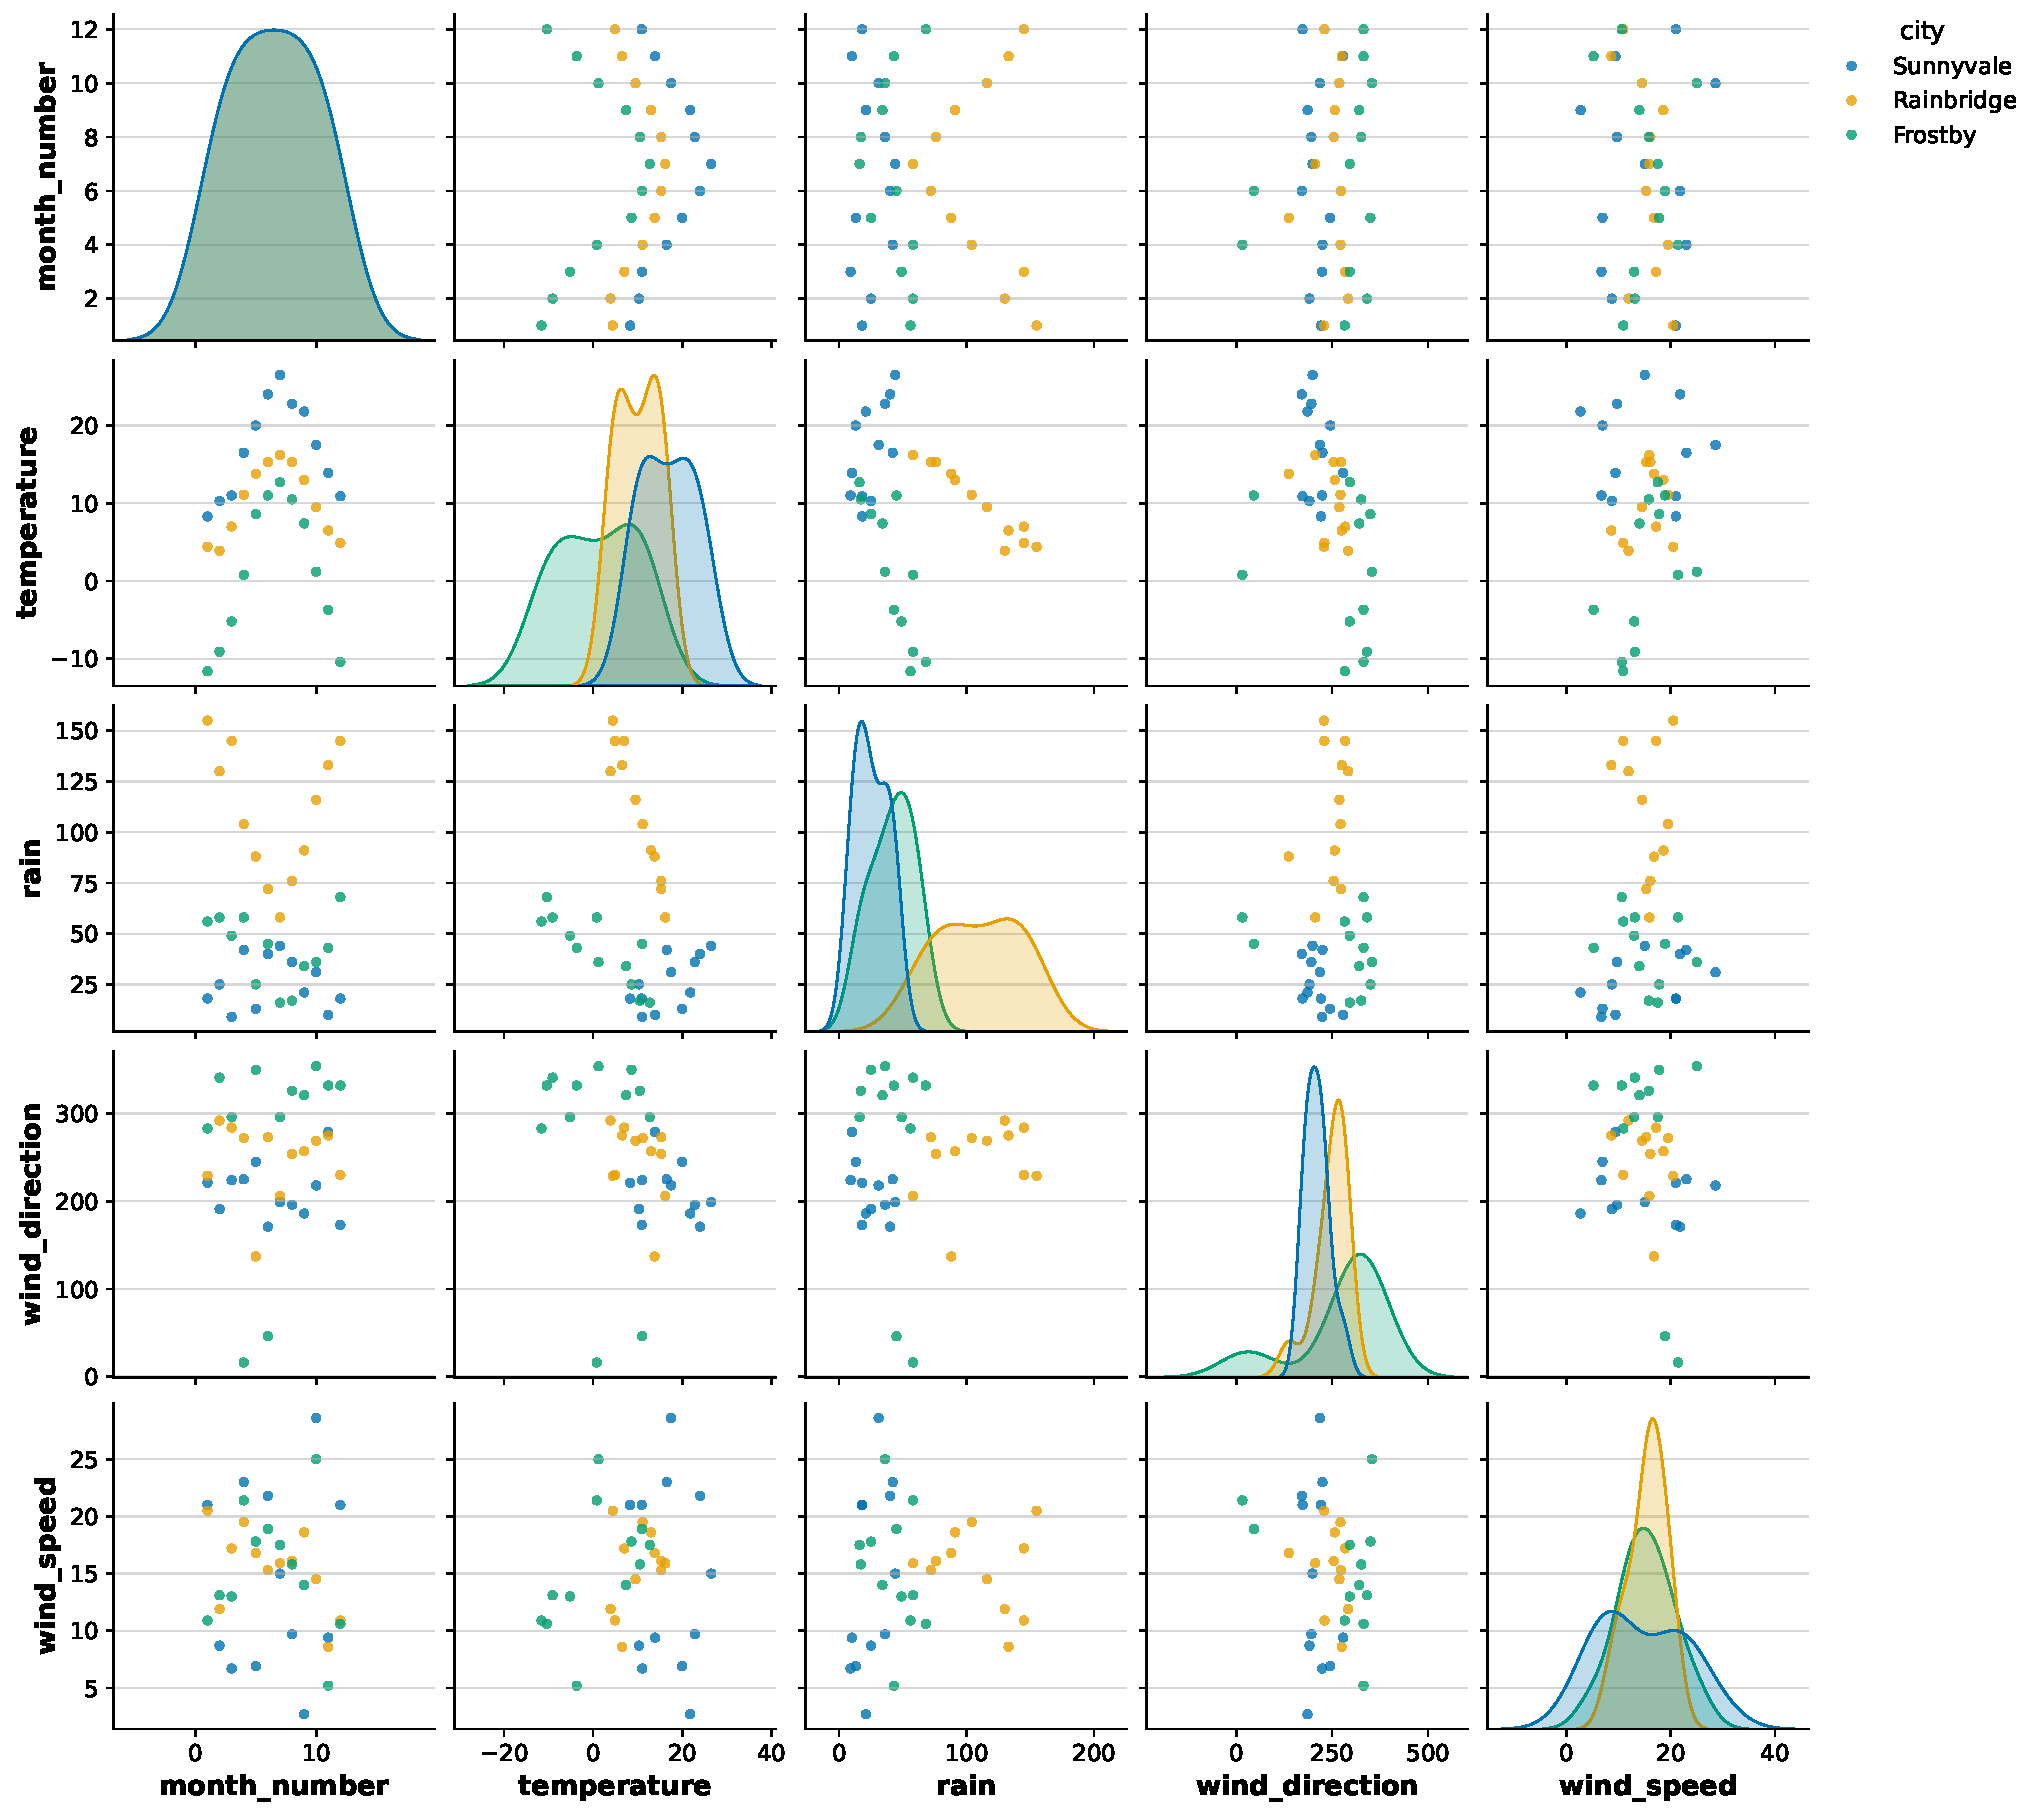
\includegraphics[width=0.52\textwidth,height=0.30\textheight,keepaspectratio]{figures/solution07_task3_lesson7_weather_pairs.pdf}
\captionof*{figure}{Lesson 7, task 3: \code{lesson7\_\allowbreak{}weather\_\allowbreak{}pairs.\allowbreak{}png}.}
\end{minipage}\end{center}
\solutionanswer{Every number column of the weather table against every other, one colour per city.}
\par\noindent{\small\sffamily\hyperref[lesson:7]{Back to lesson 7}}
\unsection{Lesson 8: Hard tricks, and your own program}{solutions:8}
\solutiontask{1}{Write your own program, from an empty file, for a question you care about.}
\begin{lstlisting}[style=py]
import simplydata as sdata
fruit = sdata.example("fruit")
print(fruit)
chart = sdata.chart(fruit)
chart.bars(x="fruit", y="count", show="total")
chart.numbers_on_bars()
chart.title_top("Which fruit sells best?")
chart.label_x("Fruit")
chart.label_y("Sold in one week")
chart.save("lesson8_fruit.png")
\end{lstlisting}
\printedoutput{output/solution08_task1.txt}
\begin{center}\begin{minipage}{\linewidth}\centering
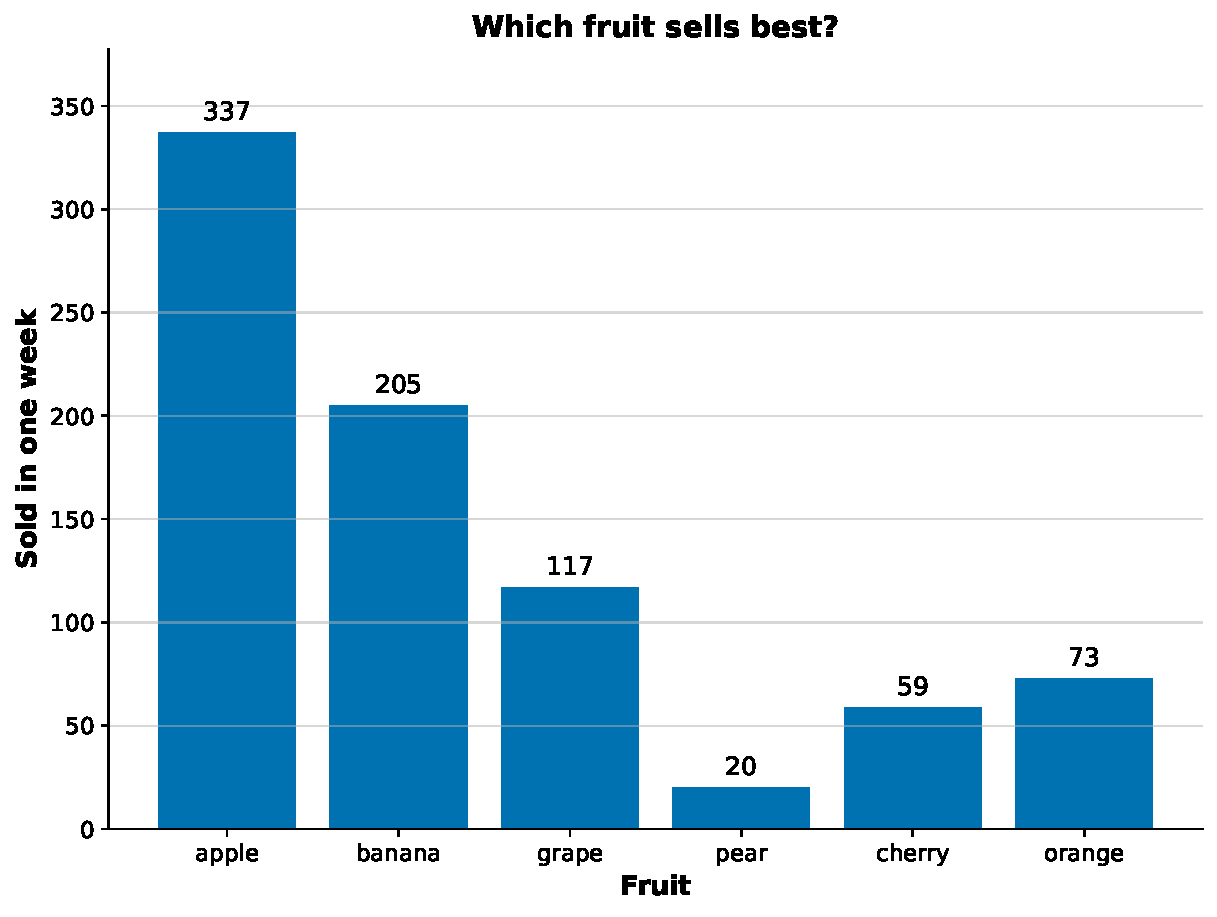
\includegraphics[width=0.52\textwidth,height=0.30\textheight,keepaspectratio]{figures/solution08_task1_lesson8_fruit.pdf}
\captionof*{figure}{Lesson 8, task 1: \code{lesson8\_\allowbreak{}fruit.\allowbreak{}png}.}
\end{minipage}\end{center}
\solutionanswer{One possible question: which fruit sells best? Same plan as always: get the data, look, start, draw, words, save.}
\solutiontask{2}{Use any example table, or your own. Give it a title, axis names and a note.}
\begin{lstlisting}[style=py]
import simplydata as sdata
growth = sdata.example("growth")
chart = sdata.chart(growth)
chart.lines(x="year", y="forest", colour="country")
chart.title_top("Forest in four countries")
chart.label_x("Year")
chart.label_y("Forest (% of the land)")
chart.note("Applia loses the most", x=2016, y=50, arrow=True)
chart.save("lesson8_forest.png")
\end{lstlisting}
\printedoutput{output/solution08_task2.txt}
\begin{center}\begin{minipage}{\linewidth}\centering
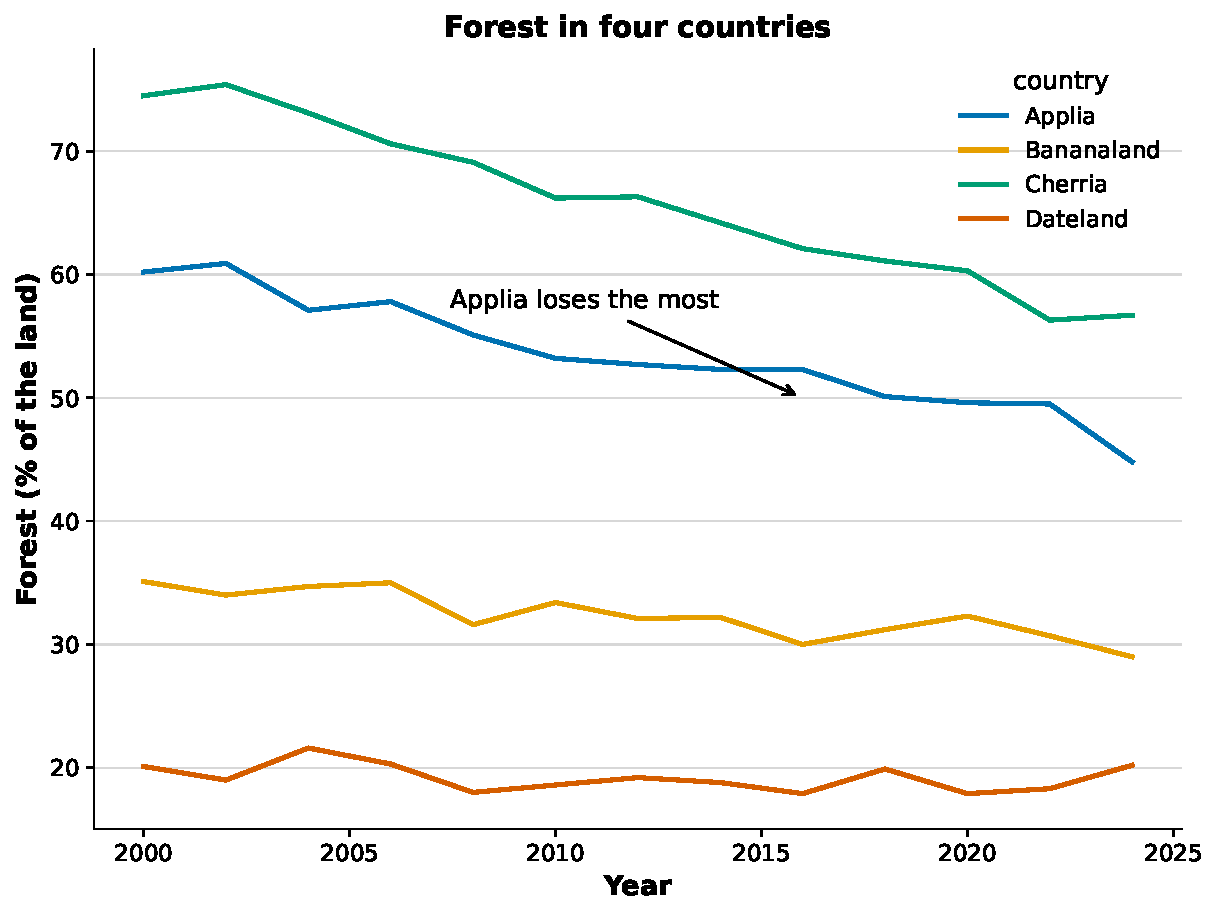
\includegraphics[width=0.52\textwidth,height=0.30\textheight,keepaspectratio]{figures/solution08_task2_lesson8_forest.pdf}
\captionof*{figure}{Lesson 8, task 2: \code{lesson8\_\allowbreak{}forest.\allowbreak{}png}.}
\end{minipage}\end{center}
\solutionanswer{Another table, with a title, both axis names and a note with an arrow.}
\solutiontask{3}{Make a second chart of the same table, put the two charts side by side and save the page as a PDF.}
\begin{lstlisting}[style=py]
import simplydata as sdata
growth = sdata.example("growth")
people = sdata.chart(growth).lines(x="year", y="population", colour="country")
people.label_y("People (millions)")
forest = sdata.chart(growth).lines(x="year", y="forest", colour="country")
forest.label_y("Forest (% of the land)")
page = sdata.side_by_side(people, forest, letters=True)
page.save("lesson8_page.pdf")
\end{lstlisting}
\printedoutput{output/solution08_task3.txt}
\begin{center}\begin{minipage}{\linewidth}\centering
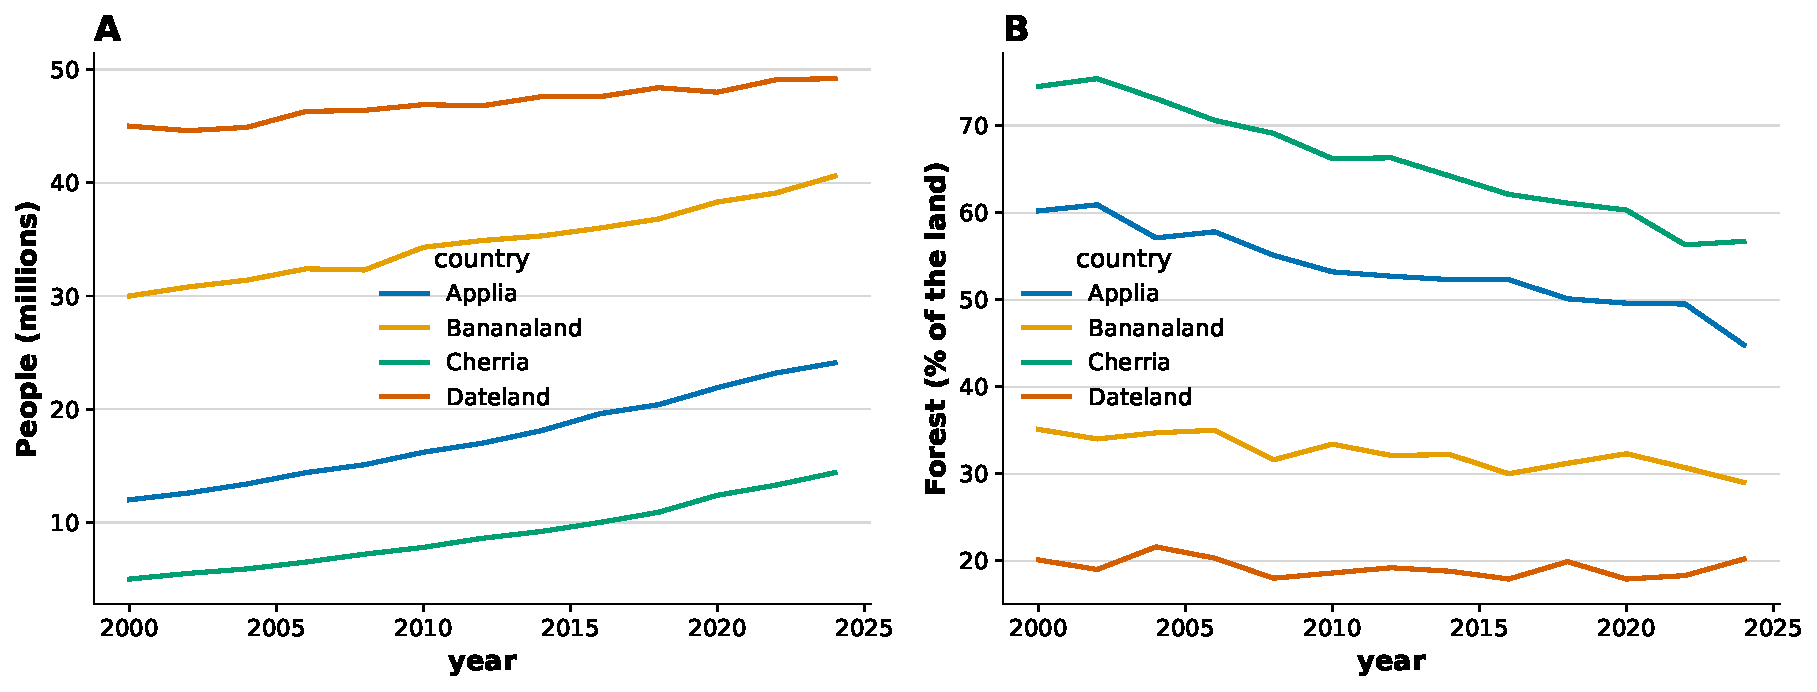
\includegraphics[width=0.52\textwidth,height=0.30\textheight,keepaspectratio]{figures/solution08_task3_lesson8_page.pdf}
\captionof*{figure}{Lesson 8, task 3: \code{lesson8\_\allowbreak{}page.\allowbreak{}pdf}.}
\end{minipage}\end{center}
\solutionanswer{Two charts of one table on one page, saved as a PDF because the name ends in \code{.\allowbreak{}pdf}.}
\par\noindent{\small\sffamily\hyperref[lesson:8]{Back to lesson 8}}
\unsection{Lesson 9: Tables: open one and look at it}{solutions:9}
\solutiontask{1}{Make a table of \code{sdata.\allowbreak{}example(\textquotedbl{}weather\textquotedbl{})}. How many rows does it have?}
\begin{lstlisting}[style=py]
import simplydata as sdata
table = sdata.table(sdata.example("weather"))
table.count_rows()
\end{lstlisting}
\printedoutput{output/solution09_task1.txt}
\solutionanswer{36 rows: 12 months for each of 3 cities.}
\solutiontask{2}{Describe its columns. Which column has the biggest numbers?}
\begin{lstlisting}[style=py]
import simplydata as sdata
table = sdata.table(sdata.example("weather"))
table.describe_columns()
\end{lstlisting}
\printedoutput{output/solution09_task2.txt}
\solutionanswer{\code{wind\_\allowbreak{}direction} has the biggest numbers (up to 354): it is an angle in degrees, from 0 to 360.}
\solutiontask{3}{Count each \code{\textquotedbl{}city\textquotedbl{}}. Does every city have the same number of rows?}
\begin{lstlisting}[style=py]
import simplydata as sdata
table = sdata.table(sdata.example("weather"))
table.count_each("city")
\end{lstlisting}
\printedoutput{output/solution09_task3.txt}
\solutionanswer{Yes: Frostby, Rainbridge and Sunnyvale have 12 rows each, one for every month.}
\par\noindent{\small\sffamily\hyperref[lesson:9]{Back to lesson 9}}
\unsection{Lesson 10: Tables: choose rows and columns, and undo}{solutions:10}
\solutiontask{1}{In the marks table, keep only class \code{\textquotedbl{}B\textquotedbl{}} and sort by \code{\textquotedbl{}hours\textquotedbl{}}. Who studied the longest?}
\begin{lstlisting}[style=py]
import simplydata as sdata
table = sdata.table(sdata.example("marks"))
table.keep_rows("class", equal_to="B")
table.sort_by("hours", biggest_first=True)
table.show_first_rows(3)
\end{lstlisting}
\printedoutput{output/solution10_task1.txt}
\solutionanswer{Jade studied the longest: 9.4 hours, for Maths. \code{biggest\_\allowbreak{}first=True} puts the longest on top.}
\solutiontask{2}{Undo the sorting, then sort by name instead.}
\begin{lstlisting}[style=py]
import simplydata as sdata
table = sdata.table(sdata.example("marks"))
table.keep_rows("class", equal_to="B")
table.sort_by("hours", biggest_first=True)
table.undo()
table.sort_by("name")
table.show_first_rows()
\end{lstlisting}
\printedoutput{output/solution10_task2.txt}
\solutionanswer{\code{undo()} takes back only the sorting; class B stays. Text is sorted from A to Z.}
\solutiontask{3}{Keep 5 random rows with \code{table.\allowbreak{}keep\_\allowbreak{}random\_\allowbreak{}rows(5,\allowbreak{} seed=1)} and save them as \code{\textquotedbl{}five.\allowbreak{}csv\textquotedbl{}}.}
\begin{lstlisting}[style=py]
import simplydata as sdata
table = sdata.table(sdata.example("marks"))
table.keep_random_rows(5, seed=1)
print(table)
table.save("five.csv")
\end{lstlisting}
\printedoutput{output/solution10_task3.txt}
\solutionanswer{\code{seed=1} picks the same 5 rows every time, so someone else can repeat it.}
\solutiontask{4}{With one written condition, keep the rows with marks below 50 or hours above 8. How many rows are there?}
\begin{lstlisting}[style=py]
import simplydata as sdata
table = sdata.table(sdata.example("marks"))
table.keep_rows("marks < 50 or hours > 8")
table.count_rows()
\end{lstlisting}
\printedoutput{output/solution10_task4.txt}
\solutionanswer{19 rows: or keeps a row when at least one of the two is true.}
\par\noindent{\small\sffamily\hyperref[lesson:10]{Back to lesson 10}}
\unsection{Lesson 11: Tables: clean the data and add new columns}{solutions:11}
\solutiontask{1}{In the first example, fill the empty marks with the median instead of the average.}
\begin{lstlisting}[style=py]
import simplydata as sdata
table = sdata.table(sdata.example("marks"))
table.replace_values("marks", [61, 73], with_value=None)
table.count_empty_cells()
table.fill_empty_cells("marks", with_the="median")
table.count_empty_cells()
\end{lstlisting}
\printedoutput{output/solution11_task1.txt}
\solutionanswer{\code{with\_\allowbreak{}the=\textquotedbl{}median\textquotedbl{}} fills each empty mark with the middle mark of the others; afterwards no cell is empty.}
\solutiontask{2}{Add a column \code{\textquotedbl{}height\_\allowbreak{}m\textquotedbl{}} with the height in metres: \code{from\_\allowbreak{}column=\textquotedbl{}height\textquotedbl{}}, \code{divide\_\allowbreak{}by=100}.}
\begin{lstlisting}[style=py]
import simplydata as sdata
table = sdata.table(sdata.example("marks"))
table.add_column("height_m", from_column="height", divide_by=100)
table.show_first_rows()
\end{lstlisting}
\printedoutput{output/solution11_task2.txt}
\solutionanswer{The height in centimetres divided by 100: 144 becomes 1.44.}
\solutiontask{3}{In the last example, add a column \code{\textquotedbl{}best\_\allowbreak{}two\textquotedbl{}} with the formula \code{\textquotedbl{}total - English\textquotedbl{}}.}
\begin{lstlisting}[style=py]
import simplydata as sdata
table = sdata.table(sdata.example("marks"))
table.keep_columns("name", "class", "subject", "marks")
table.turn_rows_into_columns(names_from="subject", values_from="marks")
table.add_column("total", "Maths + Science + English")
table.add_column("best_two", "total - English")
table.show_first_rows()
\end{lstlisting}
\printedoutput{output/solution11_task3.txt}
\solutionanswer{The formula can use a column made earlier (total); \code{best\_\allowbreak{}two} is Maths + Science.}
\solutiontask{4}{In the shop example, add a column \code{\textquotedbl{}change\textquotedbl{}} with the change in sales from the day before, \code{for\_\allowbreak{}each=\textquotedbl{}shop\textquotedbl{}} and \code{sorted\_\allowbreak{}by=\textquotedbl{}date\textquotedbl{}} (\code{add\_\allowbreak{}change\_\allowbreak{}column}).}
\begin{lstlisting}[style=py]
import simplydata as sdata
table = sdata.table(sdata.example("shop"))
table.fill_empty_cells("sales", with_the="line between neighbours", sorted_by="date", for_each="shop")
table.add_change_column("change", from_column="sales", for_each="shop", sorted_by="date")
table.show(rows=5)
\end{lstlisting}
\printedoutput{output/solution11_task4.txt}
\solutionanswer{Each change is today's sales minus yesterday's, in the same shop; the first day of each shop has nothing before it, so its change is empty.}
\par\noindent{\small\sffamily\hyperref[lesson:11]{Back to lesson 11}}
\unsection{Lesson 12: Tables: summaries, and from a table to a chart}{solutions:12}
\solutiontask{1}{Make the fruit totals \code{for\_\allowbreak{}each=\textquotedbl{}shop\textquotedbl{}} instead. Which shop sold more?}
\begin{lstlisting}[style=py]
import simplydata as sdata
table = sdata.table(sdata.example("fruit"))
totals = table.total_of("count", for_each="shop")
print(totals)
\end{lstlisting}
\printedoutput{output/solution12_task1.txt}
\solutionanswer{The Market stall sold more: 457 pieces of fruit, against 354 at the Corner shop.}
\solutiontask{2}{Work out the average temperature \code{for\_\allowbreak{}each=\textquotedbl{}city\textquotedbl{}} in the weather table and draw it as bars.}
\begin{lstlisting}[style=py]
import simplydata as sdata
table = sdata.table(sdata.example("weather"))
averages = table.average_of("temperature", for_each="city")
chart = averages.chart()
chart.bars(x="city", y="average of temperature")
chart.numbers_on_bars(decimals=1)
chart.save("lesson12_temperature.png")
\end{lstlisting}
\printedoutput{output/solution12_task2.txt}
\begin{center}\begin{minipage}{\linewidth}\centering
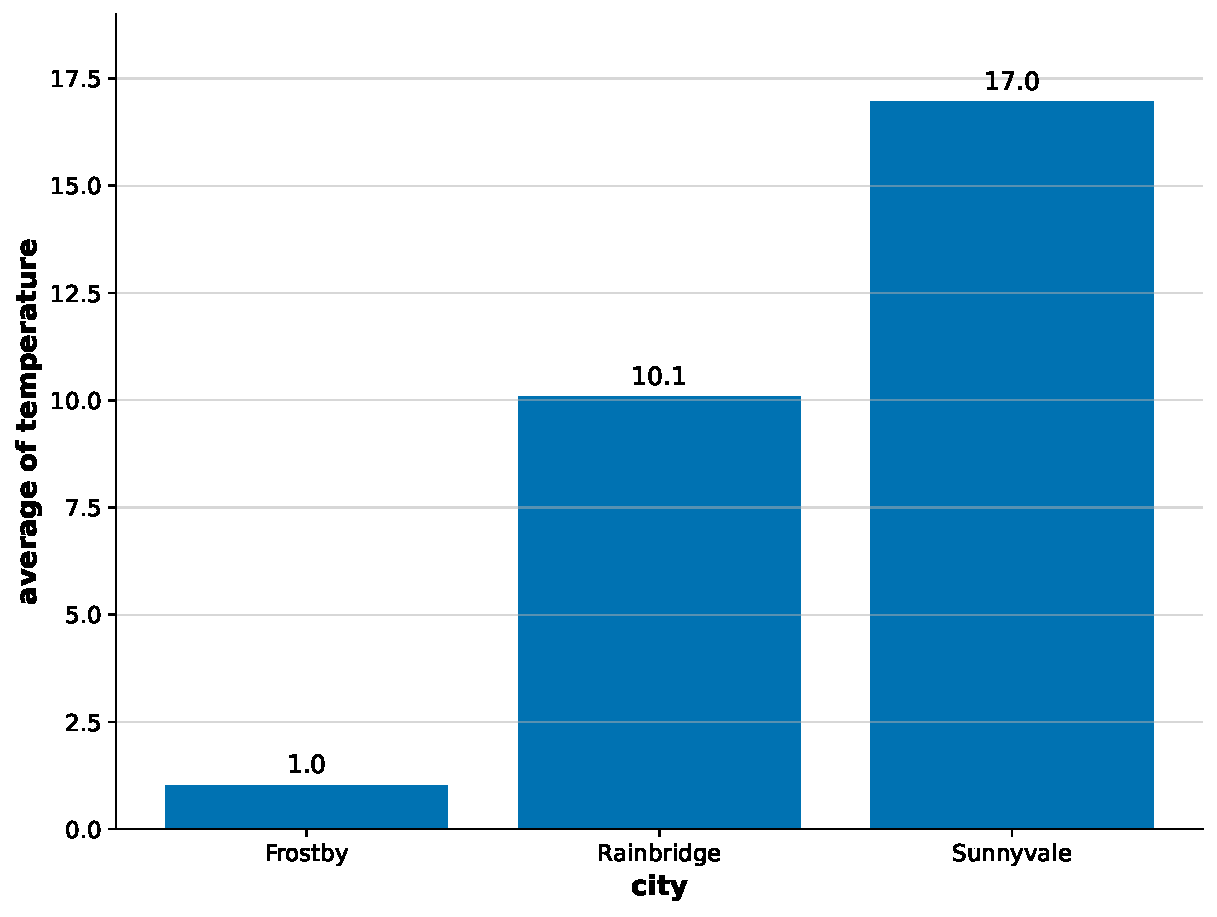
\includegraphics[width=0.52\textwidth,height=0.30\textheight,keepaspectratio]{figures/solution12_task2_lesson12_temperature.pdf}
\captionof*{figure}{Lesson 12, task 2: \code{lesson12\_\allowbreak{}temperature.\allowbreak{}png}.}
\end{minipage}\end{center}
\solutionanswer{Frostby 1.0, Rainbridge 10.1 and Sunnyvale 17.0 degrees. The summary table's column is called \code{\textquotedbl{}average of temperature\textquotedbl{}}.}
\solutiontask{3}{Is there a link between height and marks? Use \code{correlation\_\allowbreak{}between} to find out.}
\begin{lstlisting}[style=py]
import simplydata as sdata
table = sdata.table(sdata.example("marks"))
table.correlation_between("height", "marks")
\end{lstlisting}
\printedoutput{output/solution12_task3.txt}
\solutionanswer{No: r = 0.03, very close to 0, and p = 0.83 says it could easily be chance.}
\solutiontask{4}{Make a cross table of the average mark \code{for\_\allowbreak{}each=\textquotedbl{}subject\textquotedbl{}} \code{across=\textquotedbl{}class\textquotedbl{}}. Which class is best in Science?}
\begin{lstlisting}[style=py]
import simplydata as sdata
table = sdata.table(sdata.example("marks"))
table.average_of("marks", for_each="subject", across="class")
\end{lstlisting}
\printedoutput{output/solution12_task4.txt}
\solutionanswer{Class A, with an average of 79.2 in Science, against 67.5 for B and 62.3 for C.}
\par\noindent{\small\sffamily\hyperref[lesson:12]{Back to lesson 12}}
\unsection{Lesson 13: Numbers: lists and grids of numbers}{solutions:13}
\solutiontask{1}{Make the numbers 1 to 10, then square them in two ways: with ** 2 and with \code{power(2)}.}
\begin{lstlisting}[style=py]
import simplydata as sdata
nums = sdata.numbers(1, to=10)
squares = nums ** 2
print(squares)
nums.power(2)
nums.show()
\end{lstlisting}
\printedoutput{output/solution13_task1.txt}
\solutionanswer{Both give 1, 4, 9 ... 100. ** 2 makes new numbers and leaves nums alone; \code{power(2)} changes nums itself (and \code{undo()} can take it back).}
\solutiontask{2}{Make 6 dice throws with \code{sdata.\allowbreak{}random\_\allowbreak{}numbers(how\_\allowbreak{}many=6,\allowbreak{} between=[1,\allowbreak{} 6],\allowbreak{} whole\_\allowbreak{}numbers=True,\allowbreak{} seed=1)}. What is their total?}
\begin{lstlisting}[style=py]
import simplydata as sdata
dice = sdata.random_numbers(how_many=6, between=[1, 6], whole_numbers=True, seed=1)
dice.show()
dice.total()
\end{lstlisting}
\printedoutput{output/solution13_task2.txt}
\solutionanswer{With \code{seed=1} the throws are 3, 4, 5, 6, 1 and 1, which add up to 20.}
\solutiontask{3}{Make a grid of 3 rows and 4 columns filled with 0: \code{sdata.\allowbreak{}number\_\allowbreak{}grid(rows=3,\allowbreak{} columns=4,\allowbreak{} filled\_\allowbreak{}with=0)}.}
\begin{lstlisting}[style=py]
import simplydata as sdata
grid = sdata.number_grid(rows=3, columns=4, filled_with=0)
print(grid)
\end{lstlisting}
\printedoutput{output/solution13_task3.txt}
\solutionanswer{Three rows of four zeros: a grid to fill in later.}
\par\noindent{\small\sffamily\hyperref[lesson:13]{Back to lesson 13}}
\unsection{Lesson 14: Statistical tests: real difference, or chance?}{solutions:14}
\solutiontask{1}{Compare the average marks \code{for\_\allowbreak{}each=\textquotedbl{}subject\textquotedbl{}}. Could the differences be chance?}
\begin{lstlisting}[style=py]
import simplydata as sdata
table = sdata.table(sdata.example("marks"))
table.compare_averages("marks", for_each="subject")
\end{lstlisting}
\printedoutput{output/solution14_task1.txt}
\solutionanswer{Yes, they could: p = 0.26 is well above 0.05. That does not prove the subjects are the same; these data simply cannot tell.}
\solutiontask{2}{Is the average temperature different between the cities of \code{sdata.\allowbreak{}example(\textquotedbl{}weather\textquotedbl{})}?}
\begin{lstlisting}[style=py]
import simplydata as sdata
table = sdata.table(sdata.example("weather"))
table.compare_averages("temperature", for_each="city")
table.compare_each_pair("temperature", for_each="city")
\end{lstlisting}
\printedoutput{output/solution14_task2.txt}
\solutionanswer{Yes: p = 0.0002, very unlikely to be chance. \code{compare\_\allowbreak{}each\_\allowbreak{}pair} then shows which cities differ from each other.}
\solutiontask{3}{Fit a straight line of \code{\textquotedbl{}forest\textquotedbl{}} against \code{\textquotedbl{}year\textquotedbl{}} in \code{sdata.\allowbreak{}example(\textquotedbl{}growth\textquotedbl{})} for one country.}
\begin{lstlisting}[style=py]
import simplydata as sdata
table = sdata.table(sdata.example("growth"))
table.keep_rows("country", equal_to="Applia")
table.fit_line(x="year", y="forest")
\end{lstlisting}
\printedoutput{output/solution14_task3.txt}
\solutionanswer{In Applia the forest shrinks by about 0.57 percentage points a year (95 \% CI 0.48 to 0.67), and the line explains 94 \% of the differences.}
\solutiontask{4}{Remove the rows with outliers in \code{\textquotedbl{}marks\textquotedbl{}} \code{for\_\allowbreak{}each=\textquotedbl{}class\textquotedbl{}}, then compare the average marks \code{for\_\allowbreak{}each=\textquotedbl{}class\textquotedbl{}} again. Did the answer change?}
\begin{lstlisting}[style=py]
import simplydata as sdata
table = sdata.table(sdata.example("marks"))
table.remove_rows_with_outliers("marks", for_each="class")
table.compare_averages("marks", for_each="class")
\end{lstlisting}
\printedoutput{output/solution14_task4.txt}
\solutionanswer{Only one mark (33 in class B) is removed. Class B goes up from 64.3 to 66.1, but p stays 0.028: the answer does not change. Say in a report that you checked, and how.}
\par\noindent{\small\sffamily\hyperref[lesson:14]{Back to lesson 14}}
\unsection{Lesson 15: A whole analysis: from a question to a figure}{solutions:15}
\solutiontask{1}{Do a whole analysis of \code{sdata.\allowbreak{}example(\textquotedbl{}weather\textquotedbl{})}: look at it, compare the average rain \code{for\_\allowbreak{}each=\textquotedbl{}city\textquotedbl{}}, draw the rain of each city as boxes, and save the chart and the table.}
\begin{lstlisting}[style=py]
import simplydata as sdata
table = sdata.table(sdata.example("weather"))
table.describe_columns()
table.remove_columns("wind_direction", "wind_speed")
table.average_of("rain", for_each="city")
table.compare_averages("rain", for_each="city")
chart = table.chart()
chart.boxes(x="city", y="rain")
chart.all_dots(x="city", y="rain")
chart.label_y("Rain (mm)")
chart.save("lesson15_rain_boxes.png")
table.save("lesson15_weather.xlsx")
\end{lstlisting}
\printedoutput{output/solution15_task1.txt}
\begin{center}\begin{minipage}{\linewidth}\centering
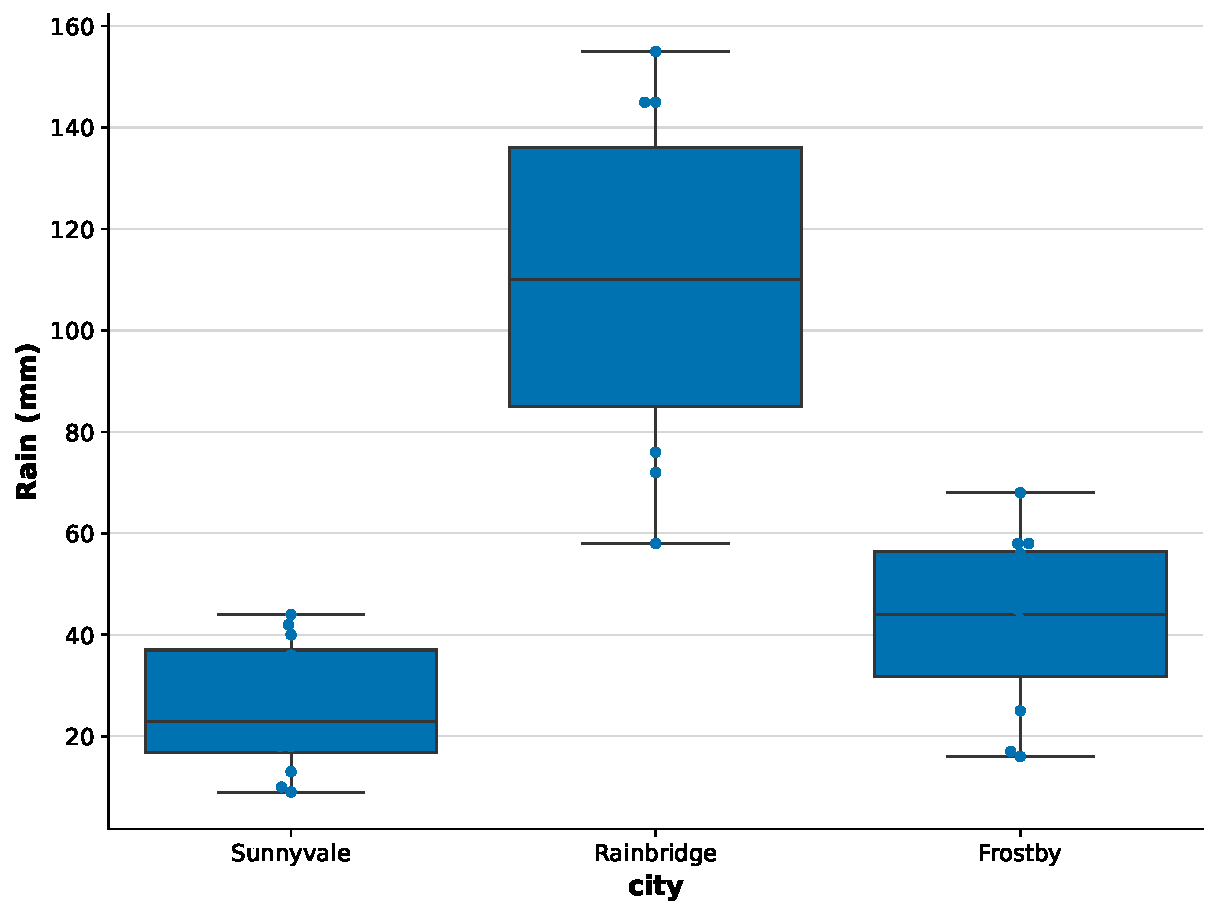
\includegraphics[width=0.52\textwidth,height=0.30\textheight,keepaspectratio]{figures/solution15_task1_lesson15_rain_boxes.pdf}
\captionof*{figure}{Lesson 15, task 1: \code{lesson15\_\allowbreak{}rain\_\allowbreak{}boxes.\allowbreak{}png}.}
\end{minipage}\end{center}
\solutionanswer{Rainbridge is much wetter (109 mm a month on average) than Frostby (42) and Sunnyvale (26); p \textless{} 0.0001, so this is very unlikely to be chance.}
\solutiontask{2}{Make a second chart of the temperature, then put the two charts together with \code{sdata.\allowbreak{}side\_\allowbreak{}by\_\allowbreak{}side(.\allowbreak{}.\allowbreak{}.\allowbreak{},\allowbreak{} letters=True)}.}
\begin{lstlisting}[style=py]
import simplydata as sdata
table = sdata.table(sdata.example("weather"))
rain = table.chart()
rain.boxes(x="city", y="rain")
rain.label_y("Rain (mm)")
warmth = table.chart()
warmth.lines(x="month", y="temperature", colour="city")
warmth.label_y("Temperature (°C)")
page = sdata.side_by_side(rain, warmth, letters=True)
page.save("lesson15_weather_page.png")
\end{lstlisting}
\printedoutput{output/solution15_task2.txt}
\begin{center}\begin{minipage}{\linewidth}\centering
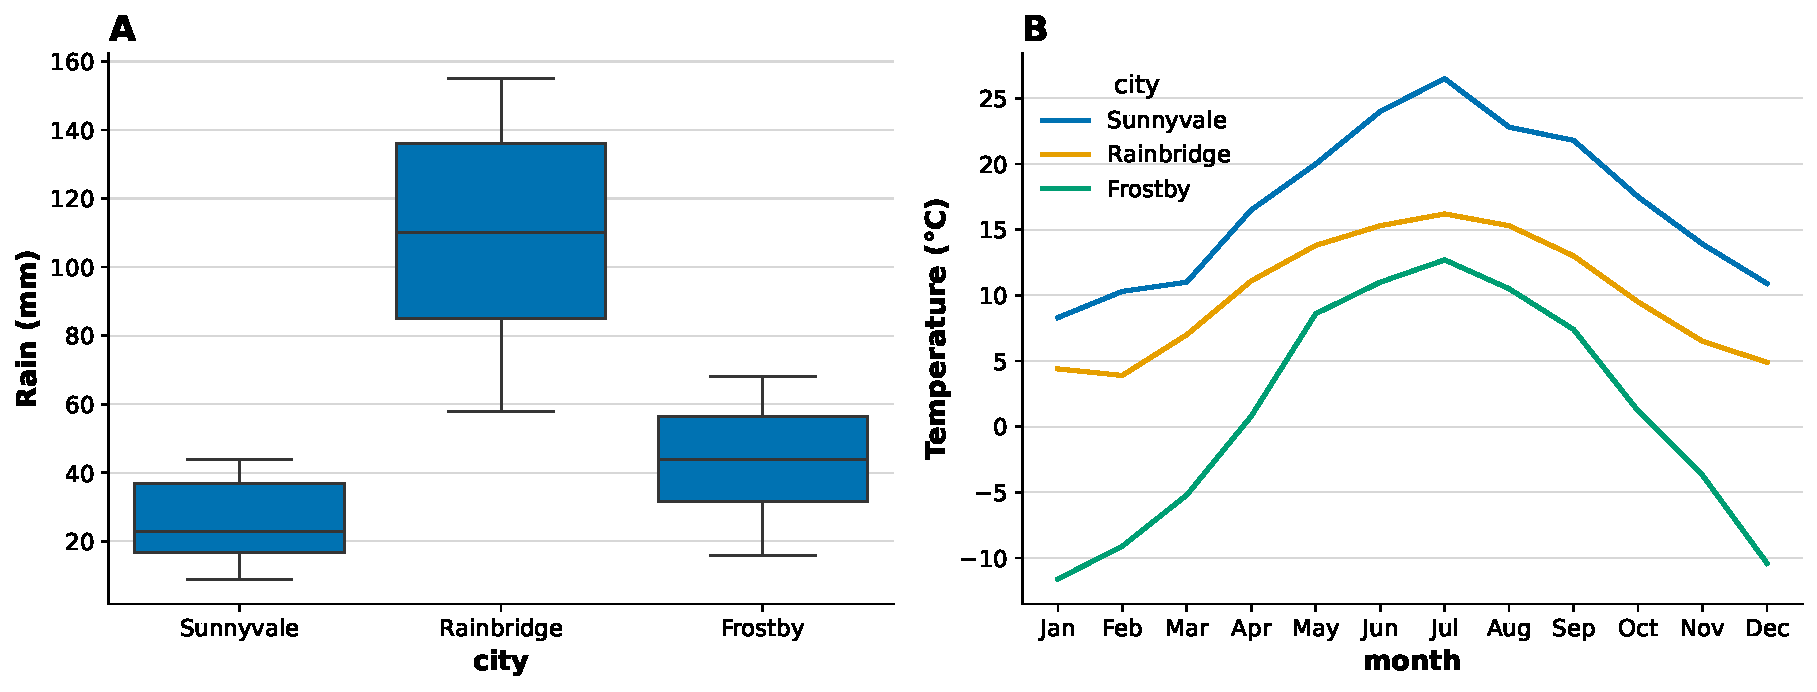
\includegraphics[width=0.52\textwidth,height=0.30\textheight,keepaspectratio]{figures/solution15_task2_lesson15_weather_page.pdf}
\captionof*{figure}{Lesson 15, task 2: \code{lesson15\_\allowbreak{}weather\_\allowbreak{}page.\allowbreak{}png}.}
\end{minipage}\end{center}
\solutionanswer{Two charts of one table, side by side, with A and B so a report can point to each.}
\solutiontask{3}{Read the \code{steps()} of your table out loud. Would someone else understand what you did?}
\begin{lstlisting}[style=py]
import simplydata as sdata
table = sdata.table(sdata.example("weather"))
table.remove_columns("wind_direction", "wind_speed")
table.keep_rows("month_number", between=[6, 8])
table.sort_by("rain", biggest_first=True)
table.steps()
\end{lstlisting}
\printedoutput{output/solution15_task3.txt}
\solutionanswer{\code{steps()} lists each change in plain words, in order; those lines are a first draft of the methods part of a report.}
\par\noindent{\small\sffamily\hyperref[lesson:15]{Back to lesson 15}}
\unsection{Lesson 16: Models: explain one column from several others}{solutions:16}
\solutiontask{1}{Explain \code{\textquotedbl{}marks\textquotedbl{}} using \code{\textquotedbl{}hours\textquotedbl{}} and \code{\textquotedbl{}school\textquotedbl{}} (school as a column of groups). Which schools differ from School A, and is school as a whole important?}
\begin{lstlisting}[style=py]
import simplydata as sdata
table = sdata.table(sdata.example("school"))
table.explain("marks", using=["hours", "school"])
\end{lstlisting}
\printedoutput{output/solution16_task1.txt}
\solutionanswer{School as a whole matters a lot (F = 10.4, p \textless{} 0.0001); School D scores about 15 marks more than School A for the same hours of study. \code{grouped\_\allowbreak{}by=} would instead treat the schools as a sample of many possible schools.}
\solutiontask{2}{Explain \code{\textquotedbl{}passed\textquotedbl{}} using \code{\textquotedbl{}hours\textquotedbl{}} and \code{\textquotedbl{}sleep\textquotedbl{}} with \code{outcome=\textquotedbl{}yes or no\textquotedbl{}}.}
\begin{lstlisting}[style=py]
import simplydata as sdata
table = sdata.table(sdata.example("school"))
table.explain("passed", using=["hours", "sleep"], outcome="yes or no")
\end{lstlisting}
\printedoutput{output/solution16_task2.txt}
\solutionanswer{Each extra hour of study multiplies the odds of passing by 1.69 and each extra hour of sleep by 1.98; both are unlikely to be chance.}
\solutiontask{3}{Explain \code{\textquotedbl{}days\_\allowbreak{}absent\textquotedbl{}} using \code{\textquotedbl{}hours\textquotedbl{}} and \code{\textquotedbl{}breakfast\textquotedbl{}} with \code{outcome=\textquotedbl{}counts\textquotedbl{}}. Does breakfast matter?}
\begin{lstlisting}[style=py]
import simplydata as sdata
table = sdata.table(sdata.example("school"))
table.explain("days_absent", using=["hours", "breakfast"], outcome="counts")
\end{lstlisting}
\printedoutput{output/solution16_task3.txt}
\solutionanswer{Breakfast could easily be chance (rate ratio 0.94, p = 0.45); study hours matter (rate ratio 0.86 for each hour).}
\par\noindent{\small\sffamily\hyperref[lesson:16]{Back to lesson 16}}
\unsection{Lesson 17: Patterns across many columns}{solutions:17}
\solutiontask{1}{Add principal components of \code{\textquotedbl{}hours\textquotedbl{}}, \code{\textquotedbl{}sleep\textquotedbl{}}, \code{\textquotedbl{}marks\textquotedbl{}} and \code{\textquotedbl{}days\_\allowbreak{}absent\textquotedbl{}} in \code{sdata.\allowbreak{}example(\textquotedbl{}school\textquotedbl{})}. Which columns weigh most in PC1?}
\begin{lstlisting}[style=py]
import simplydata as sdata
table = sdata.table(sdata.example("school"))
table.add_principal_components(columns=["hours", "sleep", "marks", "days_absent"])
\end{lstlisting}
\printedoutput{output/solution17_task1.txt}
\solutionanswer{PC1 (50 \% of the spread) is mostly hours, marks and, the other way, days absent: pupils who study more get better marks and miss fewer days. PC2 is mostly sleep.}
\solutiontask{2}{Make an NMDS map of the meadow in 3 dimensions. Is the stress lower than in 2?}
\begin{lstlisting}[style=py]
import simplydata as sdata
table = sdata.table(sdata.example("meadow"))
table.add_nmds(measure="bray-curtis", dimensions=3)
\end{lstlisting}
\printedoutput{output/solution17_task2.txt}
\solutionanswer{Yes: the stress drops from 0.195 to 0.127. That is still in the usable band (good is below 0.1), but the map keeps the distances clearly better.}
\solutiontask{3}{Do the three fields differ in make-up? Use \code{compare\_\allowbreak{}profiles} with \code{for\_\allowbreak{}each=\textquotedbl{}field\textquotedbl{}}.}
\begin{lstlisting}[style=py]
import simplydata as sdata
table = sdata.table(sdata.example("meadow"))
table.compare_profiles(for_each="field")
\end{lstlisting}
\printedoutput{output/solution17_task3.txt}
\solutionanswer{The fields explain 12 \% of the differences (p = 0.037), much less than grazing, and they do not differ in spread (p = 0.54).}
\solutiontask{4}{Cluster the meadow plots with \code{method=\textquotedbl{}hierarchical\textquotedbl{}}. Do the clusters match the grazing?}
\begin{lstlisting}[style=py]
import simplydata as sdata
table = sdata.table(sdata.example("meadow"))
table.add_clusters(how_many=2, method="hierarchical")
table.count_rows(for_each="cluster", across="grazed")
\end{lstlisting}
\printedoutput{output/solution17_task4.txt}
\solutionanswer{Exactly: cluster 1 is the 15 grazed plots and cluster 2 the 15 ungrazed ones.}
\par\noindent{\small\sffamily\hyperref[lesson:17]{Back to lesson 17}}
\unsection{Lesson 18: Survival, and planning a study}{solutions:18}
\solutiontask{1}{Explain the risk of dying from \code{\textquotedbl{}age\textquotedbl{}} alone with \code{explain\_\allowbreak{}survival}.}
\begin{lstlisting}[style=py]
import simplydata as sdata
table = sdata.table(sdata.example("trial"))
table.explain_survival(time="days", event="died", using="age")
\end{lstlisting}
\printedoutput{output/solution18_task1.txt}
\solutionanswer{Each year of age multiplies the risk by 1.05 (95 \% CI 1.03 to 1.08), p \textless{} 0.0001.}
\solutiontask{2}{How many pairs does a before/after study need to find a small change (\code{effect\_\allowbreak{}size=0.\allowbreak{}3})?}
\begin{lstlisting}[style=py]
import simplydata as sdata
sdata.how_many_needed(test="compare_before_after", effect_size=0.3)
\end{lstlisting}
\printedoutput{output/solution18_task2.txt}
\solutionanswer{90 pairs, each with a before and an after value.}
\solutiontask{3}{What is the chance to find a medium difference (\code{effect\_\allowbreak{}size=0.\allowbreak{}25}) between 3 groups with 30 values in each?}
\begin{lstlisting}[style=py]
import simplydata as sdata
sdata.chance_to_find(test="compare_averages", effect_size=0.25, groups=3, values_per_group=30)
\end{lstlisting}
\printedoutput{output/solution18_task3.txt}
\solutionanswer{Only 54 \%: too small. \code{how\_\allowbreak{}many\_\allowbreak{}needed} with \code{groups=3} tells you how many to aim for.}
\par\noindent{\small\sffamily\hyperref[lesson:18]{Back to lesson 18}}
\unsection{Lesson 19: Fitting curves, finding the best value and solving}{solutions:19}
\solutiontask{1}{Fit a curve of degree 3 to \code{\textquotedbl{}marks\textquotedbl{}} against \code{\textquotedbl{}hours\textquotedbl{}}. Does R squared go up much from the straight line?}
\begin{lstlisting}[style=py]
import simplydata as sdata
table = sdata.table(sdata.example("marks"))
table.fit_curve(x="hours", y="marks", degree=3)
\end{lstlisting}
\printedoutput{output/solution19_task1.txt}
\solutionanswer{R squared is 0.71, against 0.69 for the straight line: the extra bends add very little.}
\solutiontask{2}{With the weather table, keep the city Sunnyvale and fit \code{\textquotedbl{}temperature = a + b * cos(2 * pi * (month\_\allowbreak{}number - c) / 12)\textquotedbl{}} with \code{start=}\{\code{\textquotedbl{}a\textquotedbl{}}: 15, \code{\textquotedbl{}b\textquotedbl{}}: 8, \code{\textquotedbl{}c\textquotedbl{}}: 7\}. In which month is it warmest (c)?}
\begin{lstlisting}[style=py]
import simplydata as sdata
table = sdata.table(sdata.example("weather"))
table.keep_rows("city", equal_to="Sunnyvale")
table.fit_formula("temperature = a + b * cos(2 * pi * (month_number - c) / 12)",
                  start={"a": 15, "b": 8, "c": 7})
\end{lstlisting}
\printedoutput{output/solution19_task2.txt}
\solutionanswer{c = 7.19: the warmest time is in July; a = 17.0 is the average and b = 8.18 how far it swings.}
\solutiontask{3}{Try to remember without looking back: which word finds where a formula is biggest, and which word finds where the two sides of an equation are equal? Use them on \code{\textquotedbl{}x * (10 - x)\textquotedbl{}} between 0 and 10, and on \code{\textquotedbl{}x**2 = 2\textquotedbl{}} between 0 and 2.}
\begin{lstlisting}[style=py]
import simplydata as sdata
sdata.find_biggest("x * (10 - x)", between=[0, 10])
sdata.solve("x**2 = 2", between=[0, 2])
\end{lstlisting}
\printedoutput{output/solution19_task3.txt}
\solutionanswer{\code{find\_\allowbreak{}biggest} gives 25 at x = 5, and solve gives x = 1.41421, the square root of 2.}
\par\noindent{\small\sffamily\hyperref[lesson:19]{Back to lesson 19}}
\unsection{Lesson 20: Distributions, chances and values between points}{solutions:20}
\solutiontask{1}{Ten coins are thrown. With \code{sdata.\allowbreak{}distribution(\textquotedbl{}binomial\textquotedbl{},\allowbreak{} tries=10,\allowbreak{} chance=0.\allowbreak{}5)}, what is the chance of 8 heads or more?}
\begin{lstlisting}[style=py]
import simplydata as sdata
coins = sdata.distribution("binomial", tries=10, chance=0.5)
coins.chance(at_least=8)
\end{lstlisting}
\printedoutput{output/solution20_task1.txt}
\solutionanswer{5.47 \%: 8, 9 or 10 heads happen about once in 18 tries.}
\solutiontask{2}{Which fits the daily \code{\textquotedbl{}sales\textquotedbl{}} of the shop table best: normal, lognormal, gamma or weibull? Then check the best one with \code{compare\_\allowbreak{}shape\_\allowbreak{}to}.}
\begin{lstlisting}[style=py]
import simplydata as sdata
table = sdata.table(sdata.example("shop"))
table.compare_distributions("sales")
table.compare_shape_to("sales", "lognormal")
\end{lstlisting}
\printedoutput{output/solution20_task2.txt}
\solutionanswer{Lognormal has the smallest AIC, and its shape could well fit (p = 0.65).}
\solutiontask{3}{Try to remember without looking back: which word estimates a value between the points you measured? Use it to estimate the temperature of each city at \code{month\_\allowbreak{}number} 6.5, joined by a smooth curve.}
\begin{lstlisting}[style=py]
import simplydata as sdata
table = sdata.table(sdata.example("weather"))
estimates = table.values_at("temperature", at={"month_number": [6.5]},
                            joined_by="smooth curve", for_each="city")
estimates.show()
\end{lstlisting}
\printedoutput{output/solution20_task3.txt}
\solutionanswer{\code{values\_\allowbreak{}at} joins the months with a smooth curve and reads off each city at 6.5.}
\par\noindent{\small\sffamily\hyperref[lesson:20]{Back to lesson 20}}

\backmatter

\unchapter{Index of words}{index}
Every word and option, A to Z, with the page of its dictionary entry. Other spellings of a word (such as \code{chart.\allowbreak{}bar()} for \code{chart.\allowbreak{}bars()}) point to the same entry.
\begin{multicols}{2}\small\raggedright\setlength{\parskip}{0.1em}
\indexline{word:nums.absolute-value}{nums.absolute\_value()}
\indexline{word:nums.add}{nums.add()}
\indexline{word:table.add-adjusted-p-value-column}{table.add\_adjusted\_p\_value\_column()}
\indexline{word:table.add-change-column}{table.add\_change\_column()}
\indexline{word:table.add-clusters}{table.add\_clusters()}
\indexline{word:table.add-column}{table.add\_column()}
\indexline{word:table.add-date-part-column}{table.add\_date\_part\_column()}
\indexline{word:table.add-group-column}{table.add\_group\_column()}
\indexline{word:table.add-is-empty-column}{table.add\_is\_empty\_column()}
\indexline{word:table.add-nmds}{table.add\_nmds()}
\indexline{word:table.add-predicted-column}{table.add\_predicted\_column()}
\indexline{word:table.add-previous-value-column}{table.add\_previous\_value\_column()}
\indexline{word:table.add-principal-components}{table.add\_principal\_components()}
\indexline{word:table.add-rank-column}{table.add\_rank\_column()}
\indexline{word:table.add-rolling-column}{table.add\_rolling\_column()}
\indexline{word:table.add-rows-from}{table.add\_rows\_from()}
\indexline{word:table.add-text-part-column}{table.add\_text\_part\_column()}
\indexline{word:all-dots}{chart.all\_dots()}
\indexline{word:animate}{chart.animate()}
\indexline{word:area}{chart.area()}
\indexline{word:nums.as-numpy}{nums.as\_numpy()}
\indexline{word:table.as-pandas}{table.as\_pandas()}
\indexline{word:table.as-polars}{table.as\_polars()}
\indexline{word:dist.average}{dist.average()}
\indexline{word:nums.average}{nums.average()}
\indexline{word:table.average-of}{table.average\_of()}
\indexline{word:band}{chart.band()}
\indexline{word:bars}{chart.bar()}
\indexline{word:bars}{chart.bars()}
\indexline{word:nums.biggest}{nums.biggest()}
\indexline{word:table.biggest-of}{table.biggest\_of()}
\indexline{word:boxes}{chart.box()}
\indexline{word:boxes}{chart.boxes()}
\indexline{word:caption-bottom}{chart.caption\_bottom()}
\indexline{word:dist.chance}{dist.chance()}
\indexline{word:sdata.chance-to-find}{sdata.chance\_to\_find()}
\indexline{word:table.change-column}{table.change\_column()}
\indexline{word:dist.chart}{dist.chart()}
\indexline{word:nums.chart}{nums.chart()}
\indexline{word:sdata.chart}{sdata.chart()}
\indexline{word:table.chart}{table.chart()}
\indexline{word:colour}{chart.color()}
\indexline{word:colour-scale}{chart.color\_scale()}
\indexline{word:colours}{chart.colors()}
\indexline{word:colour}{chart.colour()}
\indexline{word:colour-scale}{chart.colour\_scale()}
\indexline{word:colours}{chart.colours()}
\indexline{word:grid.column}{grid.column()}
\indexline{word:table.column}{table.column()}
\indexline{word:table.column-names}{table.column\_names()}
\indexline{word:table.compare-average-to}{table.compare\_average\_to()}
\indexline{word:table.compare-averages}{table.compare\_averages()}
\indexline{word:table.compare-before-after}{table.compare\_before\_after()}
\indexline{word:table.compare-counts}{table.compare\_counts()}
\indexline{word:table.compare-counts-to}{table.compare\_counts\_to()}
\indexline{word:table.compare-distributions}{table.compare\_distributions()}
\indexline{word:table.compare-each-pair}{table.compare\_each\_pair()}
\indexline{word:table.compare-percent-to}{table.compare\_percent\_to()}
\indexline{word:table.compare-profiles}{table.compare\_profiles()}
\indexline{word:table.compare-shape-to}{table.compare\_shape\_to()}
\indexline{word:table.compare-spreads}{table.compare\_spreads()}
\indexline{word:table.compare-survival}{table.compare\_survival()}
\indexline{word:contour}{chart.contour()}
\indexline{word:table.correlation-between}{table.correlation\_between()}
\indexline{word:nums.count}{nums.count()}
\indexline{word:count-bars}{chart.count\_bars()}
\indexline{word:grid.count-columns}{grid.count\_columns()}
\indexline{word:table.count-different-values}{table.count\_different\_values()}
\indexline{word:nums.count-each}{nums.count\_each()}
\indexline{word:table.count-each}{table.count\_each()}
\indexline{word:table.count-empty-cells}{table.count\_empty\_cells()}
\indexline{word:nums.count-empty-numbers}{nums.count\_empty\_numbers()}
\indexline{word:grid.count-rows}{grid.count\_rows()}
\indexline{word:table.count-rows}{table.count\_rows()}
\indexline{word:cumulative-share}{chart.cumulative\_share()}
\indexline{word:curve}{chart.curve()}
\indexline{word:dist.cut-off}{dist.cut\_off()}
\indexline{word:density}{chart.density()}
\indexline{word:dist.density-at}{dist.density\_at()}
\indexline{word:table.describe-columns}{table.describe\_columns()}
\indexline{word:table.distances-between-rows}{table.distances\_between\_rows()}
\indexline{word:sdata.distribution}{sdata.distribution()}
\indexline{word:nums.divide-by}{nums.divide\_by()}
\indexline{word:dots}{chart.dots()}
\indexline{word:dots-3d}{chart.dots\_3d()}
\indexline{word:empty-cells}{chart.empty\_cells()}
\indexline{word:error-eq}{error=}
\indexline{word:error-bars}{chart.error\_bars()}
\indexline{word:sdata.example}{sdata.example()}
\indexline{word:nums.exp}{nums.exp()}
\indexline{word:table.explain}{table.explain()}
\indexline{word:table.explain-survival}{table.explain\_survival()}
\indexline{word:table.fill-empty-cells}{table.fill\_empty\_cells()}
\indexline{word:nums.fill-empty-numbers}{nums.fill\_empty\_numbers()}
\indexline{word:sdata.find-biggest}{sdata.find\_biggest()}
\indexline{word:sdata.find-smallest}{sdata.find\_smallest()}
\indexline{word:fit-curve}{chart.fit\_curve()}
\indexline{word:table.fit-curve}{table.fit\_curve()}
\indexline{word:fit-distribution}{chart.fit\_distribution()}
\indexline{word:nums.fit-distribution}{nums.fit\_distribution()}
\indexline{word:table.fit-distribution}{table.fit\_distribution()}
\indexline{word:fit-formula}{chart.fit\_formula()}
\indexline{word:table.fit-formula}{table.fit\_formula()}
\indexline{word:fit-line}{chart.fit\_line()}
\indexline{word:table.fit-line}{table.fit\_line()}
\indexline{word:flip-x}{chart.flip\_x()}
\indexline{word:flip-y}{chart.flip\_y()}
\indexline{word:font-name}{chart.font\_name()}
\indexline{word:font-size}{chart.font\_size()}
\indexline{word:sdata.grid}{sdata.grid()}
\indexline{word:heatmap}{chart.heatmap()}
\indexline{word:sdata.help}{sdata.help()}
\indexline{word:hide-grid}{chart.hide\_grid()}
\indexline{word:hide-legend}{chart.hide\_legend()}
\indexline{word:histogram}{chart.histogram()}
\indexline{word:sdata.how-many-needed}{sdata.how\_many\_needed()}
\indexline{word:table.join-with}{table.join\_with()}
\indexline{word:table.keep-biggest-rows}{table.keep\_biggest\_rows()}
\indexline{word:table.keep-columns}{table.keep\_columns()}
\indexline{word:nums.keep-first-numbers}{nums.keep\_first\_numbers()}
\indexline{word:table.keep-first-rows}{table.keep\_first\_rows()}
\indexline{word:nums.keep-last-numbers}{nums.keep\_last\_numbers()}
\indexline{word:table.keep-last-rows}{table.keep\_last\_rows()}
\indexline{word:nums.keep-numbers}{nums.keep\_numbers()}
\indexline{word:nums.keep-random-numbers}{nums.keep\_random\_numbers()}
\indexline{word:table.keep-random-rows}{table.keep\_random\_rows()}
\indexline{word:table.keep-rows}{table.keep\_rows()}
\indexline{word:table.keep-smallest-rows}{table.keep\_smallest\_rows()}
\indexline{word:label-colour-bar}{chart.label\_color\_bar()}
\indexline{word:label-colour-bar}{chart.label\_colour\_bar()}
\indexline{word:label-legend}{chart.label\_legend()}
\indexline{word:label-x}{chart.label\_x()}
\indexline{word:label-y}{chart.label\_y()}
\indexline{word:legend-bottom}{chart.legend\_bottom()}
\indexline{word:legend-left}{chart.legend\_left()}
\indexline{word:legend-right}{chart.legend\_right()}
\indexline{word:legend-top}{chart.legend\_top()}
\indexline{word:sdata.lesson}{sdata.lesson()}
\indexline{word:lines}{chart.line()}
\indexline{word:line-at-x}{chart.line\_at\_x()}
\indexline{word:line-at-y}{chart.line\_at\_y()}
\indexline{word:line-with-slope}{chart.line\_with\_slope()}
\indexline{word:lines}{chart.lines()}
\indexline{word:nums.log}{nums.log()}
\indexline{word:log-scale-x}{chart.log\_scale\_x()}
\indexline{word:log-scale-y}{chart.log\_scale\_y()}
\indexline{word:table.make-dates}{table.make\_dates()}
\indexline{word:table.make-lowercase}{table.make\_lowercase()}
\indexline{word:table.make-numbers}{table.make\_numbers()}
\indexline{word:table.make-text}{table.make\_text()}
\indexline{word:table.make-uppercase}{table.make\_uppercase()}
\indexline{word:table.map-of}{table.map\_of()}
\indexline{word:dist.median}{dist.median()}
\indexline{word:nums.median}{nums.median()}
\indexline{word:table.median-of}{table.median\_of()}
\indexline{word:dist.middle-range}{dist.middle\_range()}
\indexline{word:table.most-common-of}{table.most\_common\_of()}
\indexline{word:names-on-dots}{chart.names\_on\_dots()}
\indexline{word:note}{chart.note()}
\indexline{word:grid.number-at}{grid.number\_at()}
\indexline{word:nums.number-at}{nums.number\_at()}
\indexline{word:nums.number-grid}{nums.number\_grid()}
\indexline{word:sdata.number-grid}{sdata.number\_grid()}
\indexline{word:grid.numbers}{grid.numbers()}
\indexline{word:sdata.numbers}{sdata.numbers()}
\indexline{word:numbers-on-bars}{chart.numbers\_on\_bars()}
\indexline{word:sdata.one-above-other}{sdata.one\_above\_other()}
\indexline{word:one-chart-per}{chart.one\_chart\_per()}
\indexline{word:order-legend}{chart.order\_legend()}
\indexline{word:order-x}{chart.order\_x()}
\indexline{word:order-y}{chart.order\_y()}
\indexline{word:sdata.pairs}{sdata.pairs()}
\indexline{word:dist.parameters}{dist.parameters()}
\indexline{word:table.percent-of}{table.percent\_of()}
\indexline{word:dist.percentile}{dist.percentile()}
\indexline{word:nums.percentile}{nums.percentile()}
\indexline{word:table.percentile-of}{table.percentile\_of()}
\indexline{word:pie}{chart.pie()}
\indexline{word:polar}{chart.polar()}
\indexline{word:nums.power}{nums.power()}
\indexline{word:table.principal-components-of}{table.principal\_components\_of()}
\indexline{word:qq-dots}{chart.qq\_dots()}
\indexline{word:dist.random-numbers}{dist.random\_numbers()}
\indexline{word:sdata.random-numbers}{sdata.random\_numbers()}
\indexline{word:range-x}{chart.range\_x()}
\indexline{word:range-y}{chart.range\_y()}
\indexline{word:table.remove-columns}{table.remove\_columns()}
\indexline{word:nums.remove-duplicate-numbers}{nums.remove\_duplicate\_numbers()}
\indexline{word:table.remove-duplicate-rows}{table.remove\_duplicate\_rows()}
\indexline{word:nums.remove-empty-numbers}{nums.remove\_empty\_numbers()}
\indexline{word:table.remove-extra-spaces}{table.remove\_extra\_spaces()}
\indexline{word:nums.remove-numbers}{nums.remove\_numbers()}
\indexline{word:table.remove-rows}{table.remove\_rows()}
\indexline{word:table.remove-rows-with-empty-cells}{table.remove\_rows\_with\_empty\_cells()}
\indexline{word:table.remove-rows-with-outliers}{table.remove\_rows\_with\_outliers()}
\indexline{word:table.rename-column}{table.rename\_column()}
\indexline{word:table.replace-text}{table.replace\_text()}
\indexline{word:table.replace-values}{table.replace\_values()}
\indexline{word:nums.reverse}{nums.reverse()}
\indexline{word:rotate-labels-x}{chart.rotate\_labels\_x()}
\indexline{word:rotate-labels-y}{chart.rotate\_labels\_y()}
\indexline{word:nums.round-to}{nums.round\_to()}
\indexline{word:table.round-to}{table.round\_to()}
\indexline{word:grid.row}{grid.row()}
\indexline{word:nums.running-total}{nums.running\_total()}
\indexline{word:save}{chart.save()}
\indexline{word:nums.save}{nums.save()}
\indexline{word:table.save}{table.save()}
\indexline{word:dots}{chart.scatter()}
\indexline{word:second-y}{chart.second\_y()}
\indexline{word:shade-between-x}{chart.shade\_between\_x()}
\indexline{word:shade-between-y}{chart.shade\_between\_y()}
\indexline{word:grid.shape}{grid.shape()}
\indexline{word:show}{chart.show()}
\indexline{word:nums.show}{nums.show()}
\indexline{word:show-eq}{show=}
\indexline{word:table.show}{table.show()}
\indexline{word:nums.show-first-numbers}{nums.show\_first\_numbers()}
\indexline{word:grid.show-first-rows}{grid.show\_first\_rows()}
\indexline{word:table.show-first-rows}{table.show\_first\_rows()}
\indexline{word:show-grid}{chart.show\_grid()}
\indexline{word:nums.show-last-numbers}{nums.show\_last\_numbers()}
\indexline{word:grid.show-last-rows}{grid.show\_last\_rows()}
\indexline{word:table.show-last-rows}{table.show\_last\_rows()}
\indexline{word:show-legend}{chart.show\_legend()}
\indexline{word:table.show-rows-with-outliers}{table.show\_rows\_with\_outliers()}
\indexline{word:sdata.side-by-side}{sdata.side\_by\_side()}
\indexline{word:side-histograms}{chart.side\_histograms()}
\indexline{word:size}{chart.size()}
\indexline{word:nums.smallest}{nums.smallest()}
\indexline{word:table.smallest-of}{table.smallest\_of()}
\indexline{word:smooth-line}{chart.smooth\_line()}
\indexline{word:sdata.solve}{sdata.solve()}
\indexline{word:nums.sort}{nums.sort()}
\indexline{word:table.sort-by}{table.sort\_by()}
\indexline{word:table.split-column}{table.split\_column()}
\indexline{word:nums.square-root}{nums.square\_root()}
\indexline{word:dist.standard-deviation}{dist.standard\_deviation()}
\indexline{word:nums.standard-deviation}{nums.standard\_deviation()}
\indexline{word:table.standard-deviation-of}{table.standard\_deviation\_of()}
\indexline{word:nums.start-again}{nums.start\_again()}
\indexline{word:table.start-again}{table.start\_again()}
\indexline{word:nums.steps}{nums.steps()}
\indexline{word:table.steps}{table.steps()}
\indexline{word:style}{chart.style()}
\indexline{word:nums.subtract}{nums.subtract()}
\indexline{word:dist.summary}{dist.summary()}
\indexline{word:table.summary-of}{table.summary\_of()}
\indexline{word:surface}{chart.surface()}
\indexline{word:survival-curves}{chart.survival\_curves()}
\indexline{word:table.survival-over-time}{table.survival\_over\_time()}
\indexline{word:grid.swap-rows-and-columns}{grid.swap\_rows\_and\_columns()}
\indexline{word:dist.table}{dist.table()}
\indexline{word:nums.table}{nums.table()}
\indexline{word:sdata.table}{sdata.table()}
\indexline{word:tick-format-x}{chart.tick\_format\_x()}
\indexline{word:tick-format-y}{chart.tick\_format\_y()}
\indexline{word:ticks-x}{chart.ticks\_x()}
\indexline{word:ticks-y}{chart.ticks\_y()}
\indexline{word:nums.times}{nums.times()}
\indexline{word:title-top}{chart.title\_top()}
\indexline{word:nums.total}{nums.total()}
\indexline{word:table.total-of}{table.total\_of()}
\indexline{word:table.turn-columns-into-rows}{table.turn\_columns\_into\_rows()}
\indexline{word:table.turn-rows-into-columns}{table.turn\_rows\_into\_columns()}
\indexline{word:nums.undo}{nums.undo()}
\indexline{word:table.undo}{table.undo()}
\indexline{word:table.values-at}{table.values\_at()}
\indexline{word:dist.variance}{dist.variance()}
\indexline{word:violins}{chart.violin()}
\indexline{word:violins}{chart.violins()}
\indexline{word:sdata.words}{sdata.words()}
\indexline{word:zoom-box}{chart.zoom\_box()}
\end{multicols}

\end{document}
